% ======================================================================
% Financial Engineering and the Evidence -- master file
% "Brought into Glory" design, 7.5 x 9.25 in Kindle Direct Publishing.
%
% Build from this folder (either engine works):
%   xelatex fe ; xelatex fe ; xelatex fe      (Baskerville system font)
%   pdflatex fe; pdflatex fe; pdflatex fe     (baskervillef package)
% The index is built automatically by imakeidx.
%
% Other master files in this folder:
%   fe-agentic.tex              the "Designing Agentic AI Solutions" style
%   fe-beautybook-original.tex  the original Beautybook version
% ======================================================================
\documentclass[12pt,twoside,openany]{book}

% ---------- Output mode ----------
% true  = KDP paperback interior WITH bleed (7.625 x 9.5 in, no cover page,
%         thumb tabs run off the outer edge; choose "Bleed" when uploading)
% false = 7.5 x 9.25 in PDF with the front cover as page 1 (eBook/preview;
%         thumb tabs sit just inside the edge)
\newif\ifKDPBleed
\KDPBleedfalse

% ======================================================================
% glory-style.tex -- the "Brought into Glory" design applied to
% Financial Engineering and the Evidence.
%
% Maroon chapter tags, gold rules, maroon headings with a gold square,
% thumb tabs on the outer edge, striped tables, Baskerville at 12pt.
% Trim: 7.5 x 9.25 in for Kindle Direct Publishing (KDP).
%
% Engines:
%   xelatex  -> Baskerville (the Mac system font, as in the Glory book)
%   pdflatex -> Baskerville from the baskervillef + newtxmath packages
%               (in a full TeX Live); otherwise Latin Modern.
% The output-mode switch \ifKDPBleed is declared in fe.tex.
% ======================================================================

% ---------- where to look for \input files ---------------------------
\makeatletter
\@ifundefined{input@path}{\def\input@path{}}{}
\g@addto@macro\input@path{{./}{common/}{../common/}{chapters/}{images/}}
\makeatother

% ---------- Page size (7.5 x 9.25) ----------------------------------
% No bleed: 7.5 x 9.25 in, tabs sit 0.3 in inside the edge.
% Bleed:    7.625 x 9.5 in (0.125 in extra on the outer edge, top and
%           bottom); tabs run off the edge. Choose "Bleed" in KDP.
% Inner margin 1 in is above KDP's 0.75 in gutter for 501-700 pages.
\ifKDPBleed
\usepackage[
  paperwidth=7.625in, paperheight=9.5in,
  inner=1in, outer=0.975in,
  top=1.025in, bottom=1.025in,
  twoside
]{geometry}
\else
\usepackage[
  paperwidth=7.5in, paperheight=9.25in,
  inner=1in, outer=0.85in,
  top=0.9in, bottom=0.9in,
  twoside
]{geometry}
\fi

% ---------- Fonts ----------------------------------------------------
\usepackage{iftex}
\ifXeTeX
  \usepackage{fontspec}
  \IfFontExistsTF{Baskerville}
    {\setmainfont{Baskerville}}
    {\setmainfont{Latin Modern Roman}}% fallback when Baskerville is missing
\else
  \usepackage[T1]{fontenc}
  \IfFileExists{baskervillef.sty}
    {\usepackage{baskervillef}%
     \usepackage[varqu,varl,var0]{inconsolata}%
     \usepackage[baskervillef,vvarbb]{newtxmath}}
    {\usepackage{lmodern}}
\fi
\usepackage{microtype}
\emergencystretch=2em

% ---------- Maths, graphics, tables ---------------------------------
\usepackage{amsmath}
\ifdefined\checkmark\else\usepackage{amssymb}\fi
\usepackage{bm}
\usepackage{textcomp}
\usepackage{graphicx}
\graphicspath{{./}{images/}{cover/}{inner_pics/}}
\usepackage{etoolbox}
\PassOptionsToPackage{table,dvipsnames,svgnames}{xcolor}
\usepackage{xcolor}
\usepackage[skins,breakable]{tcolorbox}
\usepackage{eso-pic}
\usepackage{pdfpages}
\usepackage{setspace}
\usepackage[multiple]{footmisc}
\usepackage{array}
\usepackage{booktabs}
\usepackage{tabularx}
\usepackage{longtable}
\usepackage{ragged2e}
\usepackage{xurl}
\usepackage{enumitem}
\usepackage{titlesec}
\usepackage{tocloft}
\usepackage{caption}
\usepackage{fancyhdr}
\usepackage[fit]{truncate}
\usepackage{emptypage}

% ---------- TikZ and pgfplots (the book's figures) -------------------
\usepackage{tikz}
\usetikzlibrary{positioning,shapes.geometric,shapes.multipart,shapes.misc,
  arrows.meta,fit,backgrounds,calc,decorations.pathreplacing}
\usepackage{pgfplots}
\pgfplotsset{compat=1.17}
\usepgfplotslibrary{fillbetween,groupplots}
\usepackage{pgfplotstable}

% ---------- Book palette (one place for all colours) -----------------
\definecolor{FEMaroon}{RGB}{128,30,45}    % headings, tabs, header text
\definecolor{FECream}{RGB}{253,248,238}   % light backgrounds, table stripes
\definecolor{FEGold}{RGB}{196,150,60}     % rules and accents
\definecolor{reflectgreen}{HTML}{2E6B3F}
\definecolor{indepthblue}{HTML}{1F4E79}
% colours the chapter figures use
\definecolor{fenavy}{HTML}{1B2A6B}
\definecolor{fegray}{HTML}{4D4D4D}
\definecolor{feshade}{HTML}{F3F5FA}

% ---------- Typography -----------------------------------------------
\setlength{\parskip}{0.15cm}
\setlength{\parindent}{1.5em}
\linespread{1.1}
\raggedbottom
\setlist[enumerate]{itemsep=0.8pt, topsep=0pt, parsep=0pt}
\setlist[itemize]{itemsep=0.8pt, topsep=0pt, parsep=0pt}

% ---------- Float placement ------------------------------------------
\renewcommand{\topfraction}{0.85}
\renewcommand{\bottomfraction}{0.6}
\renewcommand{\textfraction}{0.1}
\renewcommand{\floatpagefraction}{0.85}
\makeatletter
\setlength{\@fptop}{0pt}
\makeatother

% ---------- Captions -------------------------------------------------
\captionsetup{labelfont={bf,color=FEMaroon}, labelsep=colon}
\captionsetup[longtable]{skip=4pt}

% ---------- Contents, List of Figures, List of Tables ----------------
\renewcommand{\cfttoctitlefont}{\hfill\Large}
\renewcommand{\cftaftertoctitle}{\hfill}
\setlength{\cftbeforechapskip}{0.6em}
\setlength{\cftchapnumwidth}{2em}
\renewcommand{\cftpartfont}{\large\bfseries\color{FEMaroon}}
\renewcommand{\cftpartpagefont}{\large\bfseries\color{FEMaroon}}
\renewcommand{\listtablename}{List of Tables}
\renewcommand{\listfigurename}{List of Figures}
\renewcommand{\cftlottitlefont}{\hfill\Large}
\renewcommand{\cftafterlottitle}{\hfill}
\renewcommand{\cftloftitlefont}{\hfill\Large}
\renewcommand{\cftafterloftitle}{\hfill}
\setlength{\cfttabnumwidth}{2.6em}
\setlength{\cftfignumwidth}{2.6em}
\setlength{\cfttabindent}{0pt}
\setlength{\cftfigindent}{0pt}

% ---------- Index ----------------------------------------------------
\usepackage{imakeidx}
\makeindex[intoc, columns=2, columnsep=1.5em, title=Index]
\indexsetup{level=\chapter*, toclevel=chapter,
  othercode={\markboth{Index}{Index}\small}}
\providecommand{\indexgroup}[1]{\par\bigskip{\large\bfseries #1}\par\nopagebreak\smallskip}

% ---------- Running heads --------------------------------------------
% Left pages: the book title. Right pages: "Chapter n Title".
% Long chapter titles are shortened with an ellipsis.
\setlength{\headheight}{16pt}
\pagestyle{fancy}
\fancyhf{}
\fancyhead[LE]{{\small\color{FEMaroon}Financial Engineering and the Evidence}}
\fancyhead[RO]{\truncate{0.9\headwidth}{\hfill\small\color{FEMaroon}\leftmark}}
\fancyfoot[LE,RO]{\textcolor{FEMaroon}{\thepage}}
\renewcommand{\headrulewidth}{0.4pt}
\renewcommand{\headrule}{{\color{FEGold}%
  \hrule width\headwidth height\headrulewidth \vskip-\headrulewidth}}
\renewcommand{\chaptermark}[1]{\markboth{Chapter \thechapter\ #1}{}}
\renewcommand{\sectionmark}[1]{}
\fancypagestyle{plain}{%
  \fancyhf{}%
  \fancyfoot[LE,RO]{\textcolor{FEMaroon}{\thepage}}%
  \renewcommand{\headrulewidth}{0pt}}

% ---------- Chapter openers ------------------------------------------
\newcommand{\ChapterTag}{%
  \tikz[baseline=(t.base)]\node[fill=FEMaroon, text=white,
    rounded corners=3pt, inner xsep=9pt, inner ysep=5pt,
    font=\Large\bfseries](t){Chapter \thechapter};}
\titleformat{\chapter}[display]
  {\SetThumbForChapter\normalfont\raggedright}
  {\ChapterTag}
  {0.9em}
  {\color{FEMaroon}\huge\bfseries\hyphenpenalty=10000\exhyphenpenalty=10000}
  [\vspace{0.5em}{\color{FEGold}\titlerule[1.5pt]}]
\titleformat{name=\chapter,numberless}[display]
  {\ClearThumbOnly\normalfont\raggedright}
  {}
  {0pt}
  {\color{FEMaroon}\huge\bfseries\hyphenpenalty=10000\exhyphenpenalty=10000}
  [\vspace{0.5em}{\color{FEGold}\titlerule[1.5pt]}]
\titlespacing*{\chapter}{0pt}{40pt}{26pt}

% Part pages: a maroon "Part n" tag, the title and a gold rule, centred.
\newcommand{\PartTag}{%
  \tikz[baseline=(t.base)]\node[fill=FEMaroon, text=white,
    rounded corners=3pt, inner xsep=11pt, inner ysep=6pt,
    font=\LARGE\bfseries](t){Part \thepart};}
\titleformat{\part}[display]
  {\SetThumbForPart\normalfont\centering}
  {\PartTag}
  {1.2em}
  {\color{FEMaroon}\Huge\bfseries\hyphenpenalty=10000\exhyphenpenalty=10000}
  [\vspace{0.8em}{\color{FEGold}\titlerule[1.5pt]}]

% ---------- Section headings: gold square, maroon, no hyphenation ----
\newcommand{\SectionMark}{\textcolor{FEGold}{\rule{0.55em}{0.55em}}\hspace{0.45em}}
\titleformat{\section}
  {\normalfont\Large\bfseries\raggedright\color{FEMaroon}}
  {\SectionMark\thesection}{0.8em}
  {\hyphenpenalty=10000\exhyphenpenalty=10000}
\titleformat{name=\section,numberless}
  {\normalfont\Large\bfseries\raggedright\color{FEMaroon}}
  {}{0pt}
  {\SectionMark\hyphenpenalty=10000\exhyphenpenalty=10000}
\titleformat{\subsection}
  {\normalfont\large\bfseries\raggedright\color{FEMaroon!80}}
  {\thesubsection}{0.8em}
  {\hyphenpenalty=10000\exhyphenpenalty=10000}
\titleformat{\subsubsection}
  {\normalfont\normalsize\bfseries\raggedright\color{FEMaroon!80}}
  {\thesubsubsection}{0.8em}
  {\hyphenpenalty=10000\exhyphenpenalty=10000}

% ---------- Tables: maroon rules, cream stripes ----------------------
% Floating tables: row 1 is the header, stripes start at row 2.
% Long tables keep the maroon rules but no stripes, because some have
% a caption row and some do not.
\AtBeginEnvironment{table}{\rowcolors{2}{white}{FECream}%
  \arrayrulecolor{FEMaroon!70}}
\AtBeginEnvironment{longtable}{\arrayrulecolor{FEMaroon!70}}

% ---------- Boxes ----------------------------------------------------
% The chapters define callout and technote only if they are missing,
% so the definitions here give every chapter the Glory look.

% "For readers new to ..." and other side notes: cream with a gold bar
\newtcolorbox{callout}{enhanced, breakable, width=\textwidth,
  colback=FECream, colframe=FEGold, boxrule=0pt, leftrule=3pt, arc=2pt,
  left=8pt, right=8pt, top=6pt, bottom=6pt,
  before skip=12pt, after skip=12pt}

% Optional technical material: the blue In-Depth frame
\newtcolorbox{technote}{enhanced, breakable, width=\textwidth,
  colback=indepthblue!5, colframe=indepthblue!80, boxrule=0.6pt, arc=2pt,
  left=8pt, right=8pt, top=6pt, bottom=6pt,
  before skip=12pt, after skip=12pt}

% Extra Glory boxes, ready for later use
\newenvironment{ReaderQuestion}[1][A Question for You]
{\begin{tcolorbox}[enhanced, breakable, width=\textwidth,
    colback=reflectgreen!6, colframe=reflectgreen!75,
    boxrule=0pt, leftrule=3pt, arc=2pt,
    left=8pt, right=8pt, top=6pt, bottom=6pt,
    before skip=12pt, after skip=12pt,
    fonttitle=\bfseries\color{reflectgreen}, coltitle=reflectgreen,
    colbacktitle=reflectgreen!6, title={#1},
    attach title to upper={\par\smallskip}]}
{\end{tcolorbox}}

\newenvironment{InDepth}[1][In-Depth Analysis]
{\begin{tcolorbox}[enhanced, breakable, width=\textwidth,
    colback=indepthblue!5, colframe=indepthblue!80, boxrule=0.6pt, arc=2pt,
    left=8pt, right=8pt, top=6pt, bottom=6pt,
    before skip=12pt, after skip=12pt,
    fonttitle=\bfseries, coltitle=white, colbacktitle=indepthblue!80,
    title={#1}]}
{\end{tcolorbox}}

% ---------- Thumb tabs on the outer page edge ------------------------
% One tab position per Part (nine parts), labelled with the chapter
% number, so all 22 chapters fit down the 9.25 in edge.
% No-bleed mode: tabs sit 0.3 in inside the edge (outside KDP's 0.25 in
% safety margin). Bleed mode: tabs run 0.125 in past the trim line.
\ifKDPBleed
  \newcommand{\ThumbInset}{0pt}\newcommand{\ThumbTopShift}{0.125in}
\else
  \newcommand{\ThumbInset}{0.3in}\newcommand{\ThumbTopShift}{0pt}
\fi
\gdef\ThumbText{}
\gdef\ThumbColor{FEMaroon}
\gdef\ThumbY{0pt}
\newcommand{\ThumbAt}[3]{% #1 = slot, #2 = colour, #3 = label
  \xdef\ThumbY{\the\dimexpr 2.2cm + \ThumbTopShift + 2.05cm*(#1-1)\relax}%
  \gdef\ThumbColor{#2}\xdef\ThumbText{#3}}
\newcommand{\SetThumbForChapter}{%
  \ifnum\value{part}>0
    \ThumbAt{\number\value{part}}{FEMaroon}{\arabic{chapter}}%
  \else\gdef\ThumbText{}\fi}
\newcommand{\SetThumbForPart}{%
  \ThumbAt{\number\value{part}}{FEGold!90!black}{\Roman{part}}}
\newcommand{\ClearThumbOnly}{\gdef\ThumbText{}}
\newcommand{\ClearThumb}{\gdef\ThumbText{}}
\tikzset{thumbtab/.style={fill=\ThumbColor, text=white,
  minimum width=1.05cm, minimum height=1.0cm, inner sep=1pt,
  font=\footnotesize\bfseries, rounded corners=2pt}}

% ---------- Physical page count (what KDP sees) ----------------------
% A physical odd page is a right-hand page; its outer edge is on the right.
\newcount\PhysPage
\AddToShipoutPictureBG{\global\advance\PhysPage by 1\relax}
% Start the next page on a right-hand page, adding a blank page if needed.
\newcommand{\ClearToRecto}{\clearpage
  \ifodd\PhysPage\null\thispagestyle{empty}\ClearThumbOnly\clearpage\fi}
\AddToShipoutPictureBG{%
  \ifx\ThumbText\empty\else
  \begin{tikzpicture}[remember picture, overlay]
    \ifodd\PhysPage
      \node[thumbtab, anchor=north east]
        at ([xshift=-\ThumbInset, yshift=-\ThumbY]current page.north east)
        {\ifKDPBleed\hspace*{0.15cm}\fi\ThumbText};
    \else
      \node[thumbtab, anchor=north west]
        at ([xshift=\ThumbInset, yshift=-\ThumbY]current page.north west)
        {\ThumbText\ifKDPBleed\hspace*{0.15cm}\fi};
    \fi
  \end{tikzpicture}\fi}

% ---------- Links (no coloured boxes, as in the Glory book) ----------
\usepackage[hidelinks]{hyperref}


\begin{document}
\frontmatter

\ifKDPBleed\else   % the paperback cover is uploaded separately to KDP
\includepdf[pages=1, fitpaper=true, scale=1]{cover/The_frontcover_75_925.pdf}
\fi

% =========================
% Front Matter
% =========================

% ----- Copyright -----
\thispagestyle{empty}
\vspace*{\fill}
\footnotesize

\noindent
\textcopyright{} 2027 Chris Kuo

\vspace{0.5cm}

\noindent
ISBN: 979-8-9825592-1-0\\
First edition: January, 2027

\vspace{0.5cm}
\noindent All rights reserved. No part of this publication may be reproduced, stored in a retrieval system, or transmitted in any form or by any means, electronic, mechanical, photocopying, recording, scanning, or otherwise, except as permitted under Section 107 or 108 of the 1976 United States Copyright Act, without the prior written permission of the publisher, or in the case of brief quotations embodied in critical reviews and certain other noncommercial uses permitted by copyright law.

While every effort has been made to ensure the reliability of the information presented in this publication, Innovation Press assumes no responsibility for errors or omissions. However, neither the author nor Innovation Press assumes any liability for damages resulting from the use of the information contained herein.

Email address: ck2869@columbia.edu

\vfill

\noindent The Innovation Press, \\
\noindent Ann Arbor, MI

\medskip
\noindent
\includegraphics[width=0.20\textwidth]{cover/innovation_press.png}
\vfill
\normalsize

% ----- About the author (on a right-hand page) -----
\ClearToRecto
\chapter*{About the Author}
\addcontentsline{toc}{chapter}{About the Author}

\textbf{Chris Kuo} is an economist, data scientist and educator with more than 25 years of experience in quantitative modeling and analytics. 
His work centers on applied artificial intelligence, machine learning and data-driven decision making. He has led data science initiatives in enterprise environments
and is the inventor of a U.S.\ patent for data-driven analytical solutions.

In addition to his industry work, Chris teaches at Columbia University and has previously taught at Boston University, the University of New Hampshire and Liberty University, in economics, management and machine learning. He believes that students learn a method best when they are asked to verify a statement with it, especially in the age of AI. That belief is the philosophy behind this book.
He has published research in economics and management journals and is the author of ten books on applied AI, machine learning and analytics.

He holds a Ph.D. in Economics from Stony Brook University and a B.S. in Nuclear Engineering from National Tsing Hua University in Taiwan. He lives in New York City with his wife.

\medskip
\noindent His published books include (by year):

\begin{enumerate}[label=\arabic*., leftmargin=*, itemsep=1pt, topsep=4pt]
  \item \textbf{2027}\quad\textit{Financial Engineering and the Evidence: Active Learning by Verifying Famous Claims}
  \item \textbf{2026}\quad\textit{Agentic AI for Anomaly Detection: Building Your Own Agentic AI Systems Step by Step}
  \item \textbf{2026}\quad\textit{Modern Causal Inference: Methods and Applications: An Essential Hands-on Guide with DoWhy, EconML, CausalML, Causal-learn in Python}
  \item \textbf{2025}\quad\textit{Introduction to Statistics with Python: The Essential Guide to Data Analysis}
  \item \textbf{2024}\quad\textit{The Handbook of Anomaly Detection (2nd Edition): Cutting-edge Methods and Hands-On Code Examples}
  \item \textbf{2024}\quad\textit{Modern Time Series Forecasting Techniques For Predictive Analytics and Anomaly Detection: From Classical Foundations to Cutting-Edge Applications}
  \item \textbf{2023}\quad\textit{The Handbook of NLP with Gensim: Leverage topic modeling to uncover hidden patterns, themes, and valuable insights within textual data}
  \item \textbf{2023}\quad\textit{The Handbook of Anomaly Detection (1st Edition): Build and modernize your anomaly detection models with examples}
  \item \textbf{2022}\quad\textit{Transfer Learning for Image Classification: With Python examples}
  \item \textbf{2022}\quad\textit{The eXplainable A.I.: With Python Examples}
  \item \textbf{2021}\quad\textit{Modern Time Series Anomaly Detection: With Python and R examples}
\end{enumerate}

% ---- Dedication -------------------------------------------------------
%\cleardoublepage
%\thispagestyle{empty}
%\vspace*{\fill}

%\begin{center}
%  \textit{This book is dedicated to Nathan and Eileen,}\\[4pt]
%  \textit{from Dad.}
%\end{center}

%\vspace{2cm}

%\noindent\rule{\textwidth}{0.8pt}
%\begin{center}
%  \begin{minipage}{0.85\textwidth}
%    \centering
%    ``Trust in the \textsc{Lord} with all your heart and lean not on your own
%    understanding; in all your ways submit to him, and he will make your
%    paths straight.''\\[6pt]
%    ---~Proverbs 3:5--6 (NIV)
%  \end{minipage}
%\end{center}
%\noindent\rule{\textwidth}{0.8pt}

%\vspace*{\fill}

% ----- Contents, figures, tables -----
\clearpage
{\setstretch{1.15}\tableofcontents}
%\clearpage
%{\setstretch{1.0}\setlength{\cftbeforefigskip}{0.4em}\listoffigures}
%\clearpage
%{\setstretch{1.0}\setlength{\cftbeforetabskip}{0.4em}\listoftables}

% =========================
% Main Matter (page 1 is a right-hand page)
% =========================
\ClearToRecto
\mainmatter

% Preface -- Financial Engineering and the Evidence
\chapter*{Preface}
\addcontentsline{toc}{chapter}{Preface}
\markboth{Preface}{Preface}

\emph{Financial Engineering and the Evidence: Active Learning by Verifying Famous Claims}


\textbf{Asset pricing}\index{asset pricing|textbf} is the study of why financial assets are worth what they are worth. An asset, such as a stock, a bond or an option, is a claim to uncertain payments in the future, and its price today must reflect both when those payments arrive and how risky they are. Asset pricing explains how markets translate future payoffs into present prices, why some assets earn higher average returns than others, and how those returns compensate investors for bearing risk. 

\section*{A natural way to learn}

For a long time I have been thinking about how people learn a technical subject, and how that learning could be more active and more inspiring.

Many textbooks follow a familiar pattern: a model is presented, its formulas are derived, a few examples are worked, and exercises follow at the end of the chapter. This is a time-tested way to pass on knowledge.

But it may not make a reader research-oriented, and it may not build the judgment a working quant needs most: knowing whether a result can be trusted. When I turn the question around and ask, ``Does this actually work? Let's find out,'' the classroom comes alive. Students make predictions, argue about what the data will show, run the numbers, and remember what they found, often because it was not what they expected.

I believe this is the natural way people learn, even in the age of AI. This book is built on that conviction. Its subtitle, \emph{Active Learning by Verifying Famous Claims}, describes the method. You will not be asked to accept the results of quantitative finance on authority. Instead, you will be invited to test those results for yourself while learning the techniques of financial engineering.

\section*{Why this approach, and why now}

Three developments make this the right moment for a book like this.

First, the evidence behind many famous claims is live and unresolved. For example, Hou, Xue and Zhang (2020) asked how many published anomalies survive when micro-caps are given little weight, and found that about 65 percent of 452 anomalies fail a basic significance test. Jensen, Kelly and Pedersen (2023) asked whether a verdict that uses the evidence from all factors at once would be kinder, and, using a Bayesian method and data from 93 countries, concluded that most factors do replicate. Goyal, Welch and Zafirov (2024) checked whether the return predictors proposed since 2008 still work, and found that many have lost their power. When leading researchers disagree, students need to be able to work through the disagreement themselves. This book is designed to bring students into such debates rather than only report their conclusions. In Chapter~\ref{ch:15}, for example, students replicate both sides of the anomaly debate and form their own view.

Second, the data to do so is now free. Kenneth French's data library, FRED, Goyal and Welch's predictor file, the Jensen--Kelly--Pedersen global factors and Chen and Zimmermann's Open Source Asset Pricing portfolios let any student rebuild published results without a paid database.

Third, new methods are entering finance faster than they are being tested. Machine learning and time series foundation models promise much, but the finance-specific evidence is mixed. Students need to learn where these tools help and where they do not, and the only way to know is to test them.

Courses that teach the replication debate usually do it through journal articles, while their textbooks present results rather than ask students to re-test them. This book is written to fill that gap.

\section*{Putting famous claims on trial}

Finance is full of famous claims. Value beats growth. Momentum works. Stock returns are predictable. Optimized portfolios beat naive ones. Machine learning finds hidden alpha.

Practitioners act on these claims, products are sold on them, and many are taught as if they were settled. They are also exactly the kind of question an active learner can answer with data.

In this book, every such claim is put on trial, and you are the one who tries it. Each claim chapter follows the same cycle:

\begin{enumerate}
  \item \textbf{Claim.} State what is asserted, in one testable sentence.
  \item \textbf{Understand.} Learn how the idea works and how the original evidence was produced.
  \item \textbf{Verify.} Rebuild the result in a Python lab on open data, then stress-test it out of sample, in other markets and after costs.
  \item \textbf{Judge.} Reach a dated verdict: survives, weakens, fails or provisional.
  \item \textbf{Apply.} Take away what investors and practitioners can use, and what remains open.
\end{enumerate}

This order is the heart of the active approach. Because the question comes first, every method is learned at the moment it is needed, to settle something you actually want to know. Newey--West errors, false-discovery rates and walk-forward evaluation stop being abstract tools and become the instruments that decide a case. Each lab also asks you to write down what you expect before you run a step. When the data disagree with your prediction, the surprise is visible, and it stays with you.

The verdicts are not foregone conclusions. Some claims largely survive, such as the predictability of volatility. Some survive only in weakened form, such as value and momentum. The goal is to follow the evidence wherever it leads, and on some questions, such as whether most published anomalies are false, serious researchers still disagree. There you will replicate both sides and write your own verdict.

Repeated across twenty-two claims, the cycle becomes a habit. That habit, more than any single verdict, is what I hope you take from this book: before believing a result, ask ``compared to what, out of sample, and after costs?''

\section*{How the book is organized}

The book has nine parts, twenty-two claim chapters and four appendices. Every chapter puts a famous claim on trial, and the chapters are ordered by two rules. Methods climb from simple to complex, so no chapter needs a method taught later. Within that ladder, the chapters follow the dates of the papers that started each claim, so the book moves from the performance tests of the 1960s to the foundation models of 2025 in roughly the order the field itself did. The one exception is Part VIII, on derivatives and credit, which comes after Part VII even though its founding papers are older. It is the most technical part of the book, and no later chapter depends on it.
Table~\ref{tab:pref-parts} lists the chapters in each part.

\begingroup
\small
\setlength{\LTpre}{6pt}\setlength{\LTpost}{6pt}
\begin{longtable}{@{}>{\raggedright\arraybackslash}p{0.07\linewidth}>{\raggedright\arraybackslash}p{0.28\linewidth}>{\raggedleft\arraybackslash}p{0.04\linewidth}>{\raggedright\arraybackslash}p{\dimexpr 0.56\linewidth-6\tabcolsep\relax}@{}}
\caption{The nine parts of the book and their chapters.}
\label{tab:pref-parts} \\
\toprule
Part & Theme & Ch. & Title \\
\midrule
\endfirsthead
\multicolumn{4}{@{}l}{\footnotesize\itshape Table~\ref{tab:pref-parts}, continued} \\
\toprule
Part & Theme & Ch. & Title \\
\midrule
\endhead
\bottomrule
\endlastfoot
I & Returns, luck and data & \ref{ch:01} & A Strong Track Record Proves Skill \\
 &  & \ref{ch:02} & Historical Data Show What a Strategy Would Have Earned \\
\addlinespace
II & The classical cross-section & \ref{ch:03} & Size and Value Explain Returns That Beta Cannot \\
 &  & \ref{ch:04} & Past Winners Keep Winning \\
\addlinespace
III & Predictability through time & \ref{ch:05} & Simple Trading Rules Beat Buy-and-Hold \\
 &  & \ref{ch:06} & Valuations Predict the Equity Premium Out of Sample \\
\addlinespace
IV & Volatility and risk & \ref{ch:07} & Volatility Is Predictable \\
 &  & \ref{ch:08} & Value-at-Risk Models Measure Risk Reliably \\
\addlinespace
V & Portfolios and dependence & \ref{ch:09} & Optimized Portfolios Beat an Equal Split Across Assets \\
 &  & \ref{ch:10} & Diversification Fails When You Need It Most \\
\addlinespace
VI & Currencies and interest rates & \ref{ch:11} & High-Interest Currencies Depreciate Enough to Offset Their Yield \\
 &  & \ref{ch:12} & Forward Rates Predict Future Interest Rates \\
\addlinespace
VII & The reckoning: costs, low risk and replication & \ref{ch:13} & A Profitable Backtest Is Profitable to Trade \\
 &  & \ref{ch:14} & Low-Risk Stocks Beat High-Risk Stocks \\
 &  & \ref{ch:15} & Most Published Anomalies Fail to Replicate \\
\addlinespace
VIII & Derivatives and credit & \ref{ch:16} & Credit Spreads Mainly Reflect Expected Defaults \\
 &  & \ref{ch:17} & Delta Hedging Removes Option Risk \\
 &  & \ref{ch:18} & Selling Options Earns a Reliable Premium \\
\addlinespace
IX & Machine learning and foundation models & \ref{ch:19} & Machine Learning Predicts Returns Better Than Linear Models \\
 &  & \ref{ch:20} & Foundation Models Forecast Better Than Classical Methods \\
 &  & \ref{ch:21} & Transformers Price Stocks Better Than Factor Models \\
 &  & \ref{ch:22} & Foundation Models Trained on Market Data Beat GARCH \\
\end{longtable}
\endgroup


Testing the claims takes you through the standard financial engineering curriculum. Each claim rests on a core model, and each chapter teaches that model in a self-contained Foundations section before testing the claim. You learn the same material as in a conventional course, but you meet each model where it makes a prediction the data can contradict.

The book can therefore stand alone or sit beside the classics. Hull, Cochrane, and Campbell, Lo and MacKinlay teach how the models are built, while this book asks whether their predictions hold.

Every chapter has a Python lab that replicates the papers behind its claim. All labs use free data, such as the Kenneth French library, FRED and Goyal and Welch's predictor file. Where an original study used a paid database, the lab explains how the free substitute differs.


\section*{Why these claims}

Each of the twenty-two claims, in Chapters~\ref{ch:01} to~\ref{ch:22}, was chosen to do two jobs at once: to settle a question that matters, and to teach a core model. The table shows how the claims map onto the standard curriculum. 

\begingroup
\small
\setlength{\LTpre}{6pt}\setlength{\LTpost}{6pt}
\begin{longtable}{@{}l>{\raggedright\arraybackslash}p{0.198\linewidth}>{\raggedright\arraybackslash}p{0.288\linewidth}>{\raggedright\arraybackslash}p{0.297\linewidth}@{}}
\toprule
Ch. & Core area & Model or tool & Claim on trial \\
\midrule
\endfirsthead
\toprule
Ch. & Core area & Model or tool & Claim on trial \\
\midrule
\endhead
\bottomrule
\endlastfoot
\ref{ch:01} & Statistics of returns & Returns, Sharpe ratio, t-statistics, luck by simulation & A strong track record proves skill \\
\ref{ch:02} & Financial data & Adjusted prices; survivorship, look-ahead and micro-cap biases & Historical data show what a strategy would have earned \\
\ref{ch:03} & Asset pricing and factors & OLS, the CAPM, factor models & Size and value explain returns that beta cannot \\
\ref{ch:04} & Market efficiency and behavior & Portfolio sorts, cross-sectional momentum, crash risk & Past winners keep winning \\
\ref{ch:05} & Technical analysis & Trading rules, time-series momentum, the Reality Check & Simple trading rules beat buy-and-hold \\
\ref{ch:06} & Forecasting and the equity premium & Walk-forward evaluation, out-of-sample $R^2$, forecast tests & Valuations predict the equity premium out of sample \\
\ref{ch:07} & Volatility modelling & ARCH/GARCH, realized and implied volatility, HAR & Volatility is predictable \\
\ref{ch:08} & Risk management & VaR, expected shortfall, backtesting, Basel & VaR models measure risk reliably \\
\ref{ch:09} & Portfolio construction & Mean--variance, efficient frontier, covariance estimation & Optimized portfolios beat an equal split across assets \\
\ref{ch:10} & Diversification and dependence & Correlation dynamics, tail dependence & Diversification fails when you need it most \\
\ref{ch:11} & International finance & Covered and uncovered interest parity, carry & High-interest currencies depreciate enough to offset their yield \\
\ref{ch:12} & Fixed income & Yield curves, forward rates, duration, expectations hypothesis & Forward rates predict future rates \\
\ref{ch:13} & Trading and implementation & Spreads, turnover, break-even costs, capacity & A profitable backtest is profitable to trade \\
\ref{ch:14} & CAPM and leverage & Security market line, Fama--MacBeth, leverage constraints & Low-risk stocks beat high-risk stocks \\
\ref{ch:15} & Econometrics of finance & Multiple testing, shrinkage, post-publication tests & Most published anomalies fail to replicate \\
\ref{ch:16} & Credit & Default, recovery, spreads, the expected-loss spread & Credit spreads mainly reflect expected defaults \\
\ref{ch:17} & Derivative pricing and hedging & Options, Black--Scholes, the Greeks, dynamic hedging & Delta hedging removes option risk \\
\ref{ch:18} & Options and volatility premia & Implied volatility, the VIX, the variance risk premium & Selling options earns a reliable premium \\
\ref{ch:19} & Machine learning & Regularization, trees, neural nets, cross-validation & Machine learning predicts returns better than linear models \\
\ref{ch:20} & Forecasting & ARIMA, exponential smoothing, zero-shot foundation models & Foundation models forecast better than classical methods \\
\ref{ch:21} & Asset-pricing theory & Stochastic discount factor, IPCA, attention & Transformers price stocks better than factor models \\
\ref{ch:22} & Financial time series and AI & Range-based volatility, fine-tuning, synthetic data & Foundation models trained on market data beat GARCH \\
\end{longtable}
\endgroup

Every claim had to pass five tests before it earned a chapter.

\begin{enumerate}
  \item \textbf{Anchored in a core model.} Testing it requires you to learn a model that belongs in any financial engineering course.
  \item \textbf{Famous and consequential.} Practitioners act on it, products are sold on it, or it shaped the research literature.
  \item \textbf{Testable with free data.} Any student can replicate the founding paper with the French library, FRED and similar public sources.
  \item \textbf{Still debated.} Recent papers disagree, so the verdict is not a foregone conclusion and your own test adds information.
  \item \textbf{A spread of verdicts.} Some claims largely survive (volatility is predictable), some survive only in weakened form (value, momentum, the option premium), and some largely fail (forward rates as forecasts, optimized portfolios beating an equal-weighted one). The method does not always say no.
\end{enumerate}

The claims do not cover everything. This is not a full treatment of stochastic calculus, exotic derivatives, term-structure models beyond the basics, corporate finance, or market microstructure at the level of the order book. 

\section*{Foundations sections by chapter}

The Foundations section in every claim chapter is part of what each chapter expects you to learn. 
The table below lists the standard texts that treat its topic in depth. You do not need the books in the Further reading column to follow this one. They are listed for readers who want a deeper treatment of a topic.

\begingroup
\small
\setlength{\LTpre}{6pt}\setlength{\LTpost}{6pt}
\begin{longtable}{@{}r>{\raggedright\arraybackslash}p{0.468\linewidth}>{\raggedright\arraybackslash}p{0.364\linewidth}@{}}
\toprule
Ch. & Foundations covers & Further reading \\
\midrule
\endfirsthead
\toprule
Ch. & Foundations covers & Further reading \\
\midrule
\endhead
\bottomrule
\endlastfoot
\ref{ch:01} & Simple, log and excess returns; the risk-free rate; expected return and volatility; the Sharpe ratio; standard errors and t-statistics & Bodie, Kane and Marcus (2024); Campbell, Lo and MacKinlay (1997) \\
\ref{ch:02} & Corporate actions and adjusted prices; index weighting; CRSP, Compustat, FRED and the French library; delisting; point-in-time data & Bodie, Kane and Marcus (2024); Bali, Engle and Murray (2016) \\
\ref{ch:03} & Describing a distribution; linear regression and the OLS assumptions & Wooldridge (2025); Bodie, Kane and Marcus (2024); Cochrane (2005) \\
\ref{ch:04} & Measuring past performance; cross-sectional and time-series momentum; volatility scaling; underreaction and overreaction & Bodie, Kane and Marcus (2024); Ilmanen (2011) \\
\ref{ch:05} & Moving-average and breakout rules; time-series versus cross-sectional momentum; volatility targeting; rule universes and the SPA test & Campbell, Lo and MacKinlay (1997); Tsay (2010) \\
\ref{ch:06} & Information sets; training, validation and test splits; why in-sample $R^2$ flatters & Hyndman and Athanasopoulos (2021); L\'opez de Prado (2018) \\
\ref{ch:07} & Volatility and variance; historical volatility and EWMA; ARCH and GARCH(1,1); realized and implied volatility & Hull (2022); Tsay (2010) \\
\ref{ch:08} & Value at Risk and expected shortfall; scaling one-day VaR to ten days; when diversification raises VaR & Hull (2022, 2023) \\
\ref{ch:09} & The investor's problem; the efficient frontier; equal weighting (1/N); why the test must be out of sample & Bodie, Kane and Marcus (2024); Luenberger (2014) \\
\ref{ch:10} & Correlation and diversification; why measured correlation rises with volatility; the Forbes--Rigobon correction; tail correlation and tail dependence; the stock--bond correlation & Bodie, Kane and Marcus (2024); Ang (2014) \\
\ref{ch:11} & Spot and forward exchange rates; covered and uncovered interest parity; the carry trade & Hull (2022); Bodie, Kane and Marcus (2024) \\
\ref{ch:12} & Zero-coupon yields; forward rates; holding-period returns; duration; the expectations hypothesis & Hull (2022); Tuckman and Serrat (2022) \\
\ref{ch:13} & The order book; market and limit orders; who provides liquidity; long and short positions; long--short portfolios; turnover & Harris (2003); Bodie, Kane and Marcus (2024); Hull (2022) \\
\ref{ch:14} & Beta, the CAPM and the security market line; alpha & Bodie, Kane and Marcus (2024); Ang (2014) \\
\ref{ch:15} & The efficient market hypothesis; the joint-hypothesis problem; anomalies; replication, reproduction and robustness; publication bias; shrinkage & Bodie, Kane and Marcus (2024); Bali, Engle and Murray (2016) \\
\ref{ch:16} & Credit spreads; default probability and recovery; the expected-loss spread; why spreads can exceed expected losses & Hull (2022) \\
\ref{ch:17} & Payoffs and put--call parity; the Black--Scholes--Merton model; the Greeks; implied volatility; delta hedging and its profit and loss; discrete hedging; the volatility smile & Hull (2022); Shreve (2004) \\
\ref{ch:18} & The VIX; the option seller's payoff & Hull (2022) \\
\ref{ch:19} & Time-series and cross-sectional questions; a simple factor model; why not use every predictor; overfitting and the bias--variance trade-off & James, Witten, Hastie and Tibshirani (2021); Hastie, Tibshirani and Friedman (2009); L\'opez de Prado (2018) \\
\ref{ch:20} & Classical benchmarks; foundation models; contamination; fair evaluation & Hyndman and Athanasopoulos (2021) \\
\ref{ch:21} & The stochastic discount factor and the tangency portfolio; shrinkage SDFs and IPCA; deep SDFs; attention and the transformer & Cochrane (2005); Bali, Engle and Murray (2016) \\
\ref{ch:22} & OHLCV bars; range-based volatility; tokenizing bars; fine-tuning; synthetic market data; the Giacomini--White test & Hull (2022); Tsay (2010) \\
\end{longtable}
\endgroup

Full references for these books are listed alphabetically under Further Reading at the end of the book (page~\pageref{furtherreading}).


\section*{Who this book is for}

This book is for anyone who builds, buys or studies quantitative strategies and needs to judge whether the evidence behind them holds up.
Students in financial engineering, quantitative finance and financial data science will use the whole book, labs included, as will quantitative analysts and researchers at asset managers, banks and fintech firms.
PhD students can use it as a companion for the replication debate. Portfolio managers, allocators and serious individual investors can read the principles and verdicts and skim the labs.

You will need to possess basic Python, and to know introductory statistics, regression and the elements of investments. Everything else is taught along the way.

\section*{How to use this book}

The book covers a wide range of financial engineering. 
A one-semester course can follow Parts I to VII and Part IX in order. Instructors can treat Part VIII, on derivatives and credit, as optional. 

\section*{An invitation}

Learning by verifying is slower at first than learning by reading. You will make predictions that turn out wrong, and you will spend time on results that do not hold. But you will understand each method because you needed it, and you will remember each verdict because you reached it yourself.

I wrote this book in the hope that it makes learning financial engineering more active and more enjoyable. Pick a claim, write down what you expect, and let the evidence decide.

\bigskip
\begin{flushright}
\emph{Chris Kuo}\\
\emph{January 2027}
\end{flushright}


% ---- Part I: Returns, Luck and Data
\part{Returns, Luck and Data}
% Chapter 1 -- Claim: A Strong Track Record Proves Skill
% Requires: amsmath, booktabs, array, tabularx, graphicx, tcolorbox (breakable, skins), hyperref or url.
% Defines the callout box only if the preamble has not.
\providecolor{fenavy}{HTML}{1B2A6B}
\providecolor{feshade}{HTML}{F3F5FA}
% Key terms are marked with \term{...}. The style is set once, in the
% preamble; this fallback uses italics if the preamble has not defined it.
\providecommand{\term}[1]{\emph{#1}}
\makeatletter
\@ifundefined{callout}{%
  \newtcolorbox{callout}{breakable, enhanced,
    colback=white, colframe=gray!70, boxrule=0.5pt, arc=1mm,
    borderline west={2.5pt}{0pt}{gray!70},
    left=8pt, right=8pt, top=4pt, bottom=4pt}%
}{}
% Shaded box for optional technical material that general readers may skip.
\@ifundefined{technote}{%
  \newtcolorbox{technote}{breakable, enhanced,
    colback=feshade, colframe=fenavy!60, boxrule=0.5pt, arc=1mm,
    left=8pt, right=8pt, top=4pt, bottom=4pt}%
}{}
\makeatother

\chapter{Claim: A Strong Track Record Proves Skill}
\label{ch:01}

Most people meet the question of this chapter long before they study finance. A friend mentions that he doubled his money on a stock he picked himself, a coworker swears by a newsletter that called the last market crash, and you may also have seen a \term{mutual fund} advertise that it has beaten the market five years in a row.
Each of these situations raises the same question: does a good record show that the person behind it knows better, or did that person simply get lucky? But we also know the small print on almost every fund advertisement. It warns that past performance is no guarantee of future results.

\term{Empirical finance} is the branch of finance that tests ideas about markets against real data, such as decades of stock prices, fund returns and interest rates.
Whether a good record reveals skill is also one of the oldest questions in empirical finance. In the 1960s mutual funds, which pool the savings of many investors and pay a professional manager to choose the stocks, sold themselves on their past returns. At the same time, the newly developed \term{Capital Asset Pricing Model (CAPM)}, which links the return an investor should expect from an investment to how strongly it moves with the overall market, gave researchers a way to ask whether those returns were more than the reward for bearing market risk. Jensen (1968) applied it to 115 mutual funds over 1945--1964. After expenses, the funds as a group earned less than a \term{buy-and-hold} position in the market with the same risk, and very few individual funds did better than chance would allow. In plain terms, the typical fund investor would have done better by buying a slice of the whole market and simply holding it. Jensen's measure, the intercept of a \term{regression} of a fund's \term{excess return} on the market's, is still called \term{Jensen's alpha}\index{alpha!Jensen's}. In everyday language, \term{alpha} is the extra return a manager earns beyond what the market alone would have delivered, and it is the yardstick for skill throughout this book.

The question matters because the answer decides how money is managed. If a long record reveals skill, investors can find good managers by studying their past returns, and paying a manager to pick stocks, which is called \term{active management}, is sensible. If it does not, much of what investors pay for is luck, and a low-cost \term{index fund}, which simply holds every stock in a \term{market index} such as the S\&P~500, is the better choice. The statistics are harder than they look. Returns are noisy, histories are short, and thousands of managers and strategies are compared at once, so the best record among many is mostly the product of chance. A simple analogy shows why. If a thousand people each flip a coin ten times, chances are that one of them will flip ten heads in a row, yet nobody would call that person a skilled coin flipper. When thousands of fund managers compete, some of them will produce dazzling records in the same way. Fama and French (2010) returned to Jensen's question for this reason, asking whether the stars among thousands of modern funds outnumber what luck alone would produce, and they confirmed that few fund managers show enough skill to cover their costs. Bailey, Borwein, L\'opez de Prado and Zhu (2014) saw the same danger in backtests, which apply a trading rule to historical prices to see how it would have performed. They showed that because a researcher can try thousands of variations of a rule and report only the best one, the winning backtest can look impressive even when the rule has no value. Harvey, Liu and Zhu (2016) noted that the field had by then tested hundreds of factors against the usual bar, and argued that it should therefore demand stronger evidence before accepting a new result.

The implications run through the rest of this book. Every claim that follows is supported by some record of past returns, and every one of them faces the same question: how much of the record is luck? The claim on trial\index{claims-on-trial method} in this chapter is the one every strategy builder hopes is true: \textbf{a long enough track record can reveal real skill.} Testing it means learning how long ``long enough'' is, and what else a record must show. The chapter also introduces the method the rest of the book uses: state the claim, understand it, verify it, judge it, and apply what survives.

The chapter draws on four papers. Jensen (1968) and Fama and French (2010) test whether fund managers beat chance; their fund data are not free, so their results are discussed rather than rerun. Bailey et al.\ (2014) show how the best of many backtests misleads, and Harvey, Liu and Zhu (2016) ask how high the statistical bar must be. The lab in Section~\ref{sec:01-lab} replicates the logic of these papers with free data: it runs 1,000 strategies with no skill at all on the U.S. market since 1926, in order to measure how good a track record luck alone can produce, and how much higher the bar must be before a record counts as evidence of skill. A strategy here is simply a rule that decides, month by month, whether to own the stock market or to keep the money in safe \term{Treasury bills}.

By the end of the chapter you will be able to:

\begin{itemize}
  \item compute simple, log and excess returns\index{return!excess}, and convert monthly means and volatilities\index{volatility} to annual ones;
  \item calculate a Sharpe ratio\index{Sharpe ratio} and judge whether a mean return is statistically different from zero;
  \item distinguish profits that come from bearing risk, from luck and from skill, and measure skill as alpha\index{alpha};
  \item explain what market efficiency\index{efficient market hypothesis} implies for return predictability\index{return predictability}, and what it does not;
  \item calculate how many years of data are needed to tell a good strategy from luck;
  \item list the main ways a backtest can mislead;
  \item use the book's claims-on-trial method and verdict scale\index{verdict scale}.
\end{itemize}

In the lab you will generate 1,000 trading strategies that are random by construction, run them on nearly a century of real U.S. market data, and watch several of them look like the work of a genius. Because you know that every one of them is pure luck, you will see exactly what a real record must do to stand out from luck. That is the best preparation for judging and building the strategies you will meet in the rest of the book and in your career.

\begin{callout}
\textbf{For readers new to the stock market.} The chapter uses a handful of everyday market terms, and readers who already know them can skip ahead to Section~\ref{sec:01-foundations}. A \term{share of stock} is a small piece of ownership in a company, and its price rises and falls as investors change their views about the company's future profits. Some companies also pay part of their profits to shareholders as a \term{dividend}. A \term{stock market index}, such as the S\&P~500, tracks the combined value of a large group of stocks, in this case about 500 of the largest U.S. companies, so when the news reports that ``the market'' rose 1\% today, it usually means that an index rose 1\%. A mutual fund pools money from many investors and invests it on their behalf. An \term{actively managed fund} pays a manager to pick stocks in the hope of beating the index, while an index fund simply buys all the stocks in the index and charges a much lower fee. A Treasury bill is a short-term loan to the U.S. government, and because the government is all but certain to repay it, its interest rate serves as the return an investor can earn without taking any risk. Finally, \term{risk} in this book means how much an investment's returns bounce around from year to year, which is why a stock that rises 30\% one year and falls 20\% the next is called riskier than a savings account, even if it ends up ahead.
\end{callout}



\section{Foundations: returns, risk and the Sharpe ratio}
\label{sec:01-foundations}

\subsection{Returns}

The \term{simple return}\index{return!simple|textbf} on an asset over a period is the gain in price plus any income, divided by the starting price:
\begin{equation}
  R_t = \frac{P_t + D_t - P_{t-1}}{P_{t-1}}
  \label{eq:01-return}
\end{equation}
where $P$ is the price and $D$ is any dividend or coupon paid during the period. For example, if you buy a share for \$100, receive a \$2 dividend during the year, and the share is worth \$108 at the end of the year, your simple return is $(108 + 2 - 100)/100 = 10$\%. A return that includes income is a \term{total return}\index{return!total|textbf}; one that does not is a \term{price return}. General readers can think of the log return, introduced next, as a bookkeeping device that makes returns easier to add up over time; it is almost the same as the simple return whenever returns are small. The \term{log return}\index{return!log|textbf}, $r = \ln(1 + R)$, is convenient because log returns add over time: the log return over a year is the sum of the twelve monthly log returns. Simple returns, by contrast, compound: \$1 grows to $(1 + R_1)(1 + R_2)\cdots(1 + R_n)$.

\subsection{The risk-free rate and excess returns}
\label{sec:01-rf}

The return on a short-term government bill, such as a one-month U.S. Treasury bill, is treated as the \term{risk-free rate}\index{risk-free rate|textbf}, $R_f$: it is known in advance and carries essentially no default risk. 
The excess return\index{return!excess|textbf} of an asset is its return minus the risk-free rate. If $R_{i,t}$ denotes the return on asset $i$ in period $t$ and $R_{f,t}$ denotes the risk-free rate for the same period, the excess return is
\begin{equation}
R^{e}_{i,t} = R_{i,t} - R_{f,t}.
\label{eq:excess-return}
\end{equation}
Excess returns measure what an investor earns for bearing risk, and most of finance is about them. Following Cochrane (2005), this book writes an excess return as $R^{e}$ and reserves a lowercase $r$ for log returns.

The average excess return of the stock market over bills is the \term{equity premium}\index{equity premium|textbf}. Writing $R_{m,t}$ for the return on the market portfolio, the equity premium is
\begin{equation}
E\left[R^{e}_{m,t}\right] = E\left[R_{m,t} - R_{f,t}\right],
\label{eq:equity-premium}
\end{equation}
and its sample estimate over $T$ periods is
\begin{equation}
\bar{R}^{e}_{m} = \frac{1}{T}\sum_{t=1}^{T} R^{e}_{m,t} = \frac{1}{T}\sum_{t=1}^{T}\left(R_{m,t} - R_{f,t}\right).
\label{eq:equity-premium-sample}
\end{equation}




\subsection{Expected return and volatility}
\label{sec:01-expret}

An asset's \term{expected return}\index{return!expected|textbf}, $E[R]$, is the average return an investor anticipates; it is never observed directly and must be estimated from history or from a model. Risk is usually measured by the \term{standard deviation}\index{standard deviation|textbf} of returns, called \term{volatility}\index{volatility|textbf}. In everyday terms, volatility is the size of a typical swing around the average: a volatility of 20\% means that a year in which stocks land 20 points above or below their usual return is entirely ordinary. Monthly figures are converted to annual ones by multiplying the mean by 12 and the standard deviation by $\sqrt{12}$, which assumes returns in different months are uncorrelated. For U.S. stocks over the last century, the annual equity premium has averaged roughly 6 to 8 percent with volatility near 20 percent, so a single year's return tells us very little about the expected return.

\subsection{Why one year tells us so little}

The problem is the size of the noise relative to the signal. Take an expected excess return of 7\%, the middle of that range, and a volatility of 20\%. The volatility is almost three times the expected return, so the randomness in any single year swamps the reward we are trying to measure. Figure~\ref{fig:01-oneyear} shows the range of outcomes this implies.

\begin{enumerate}
  \item \textbf{Ordinary years are far from the average.} About two years in three fall within one standard deviation of the expected return, between $7 - 20 = -13$\% and $7 + 20 = 27$\%. A gain of 27\% and a loss of 13\% are both ordinary years, even though the expected return is the same 7\% in each.
  \item \textbf{Large swings are normal.} About 95\% of years fall within two standard deviations, $7 \pm 1.96 \times 20$, or roughly $-32$\% to 46\%. A year like 2008, when U.S. stocks fell by more than a third, lies just beyond this range. Such a year is rare, but it is not out of character for a market this volatile.
  \item \textbf{Losing years are common.} Even though stocks are expected to beat bills by 7\% a year, 
  the excess return is negative in about 36\% of years, or roughly one year in three. A single bad year is therefore no evidence that the equity premium has disappeared, and a single good year is no evidence that it is large.
  \item \textbf{Averaging helps, but slowly.} Averaging over $T$ years shrinks the noise in the estimate to $20/\sqrt{T}$ percent. After 10 years the standard error is still about 6.3\%, so the average could plausibly lie anywhere from about $-5$\% to 19\%. Even after 100 years it is 2\%, giving a 95\% range of about 3\% to 11\%. This is why, after a century of data, researchers can say only that the equity premium is ``roughly 6 to 8 percent'' rather than give a precise number.
\end{enumerate}

The same arithmetic, applied to the \term{Sharpe ratio} rather than the average return, is what makes strategies so hard to evaluate in Section~\ref{sec:01-signal-noise}.

\providecolor{fenavy}{HTML}{1B2A6B}

\begin{figure}[!htbp]
  \centering
  \begin{tikzpicture}[
    % One-year excess return ~ Normal(mean 7%, s.d. 20%)
    declare function={
      mu = 7; sd = 20;
      pdf(\x) = exp(-0.5*((\x-mu)/sd)^2)/(sd*sqrt(2*pi));
    }]
  \begin{axis}[
    width=0.82\linewidth, height=0.42\linewidth,
    axis lines=left,
    axis line style={-stealth, thin},
    xmin=-63, xmax=77, ymin=0, ymax=0.023,
    xtick={-53,-33,-13,7,27,47,67},
    ytick=\empty,
    xlabel={One-year excess return (\%)},
    ylabel={Likelihood},
    samples=200, domain=-63:77,
    clip=false,
  ]
    \addplot[name path=dens, draw=none] {pdf(x)};
    \path[name path=base] (axis cs:-63,0) -- (axis cs:77,0);

    % Plus or minus one standard deviation: -13% to 27%
    \addplot[fill=fenavy!22, draw=none]
      fill between[of=dens and base, soft clip={domain=-13:27}];
    % Below zero
    \addplot[fill=gray!60, fill opacity=0.6, draw=none]
      fill between[of=dens and base, soft clip={domain=-63:0}];

    % Edges of the one-sigma band
    \draw[fenavy] (axis cs:-13,0) -- (axis cs:-13,{pdf(-13)});
    \draw[fenavy] (axis cs:27,0)  -- (axis cs:27,{pdf(27)});

    % Density curve on top
    \addplot[fenavy, thick] {pdf(x)};

    % Expected return
    \draw[thick, dashed] (axis cs:7,0) -- (axis cs:7,0.0215)
      node[above] {expected 7\%};

    % Labels
    \node[anchor=west] at (axis cs:-64,0.0122) {below zero: 36\%};
    \node[fenavy, anchor=west] at (axis cs:25,0.0165)
      {$\pm 1\sigma$: $-13\%$ to $27\%$};
  \end{axis}
  \end{tikzpicture}
  \caption{A single year says little about how good the stock market is, because ordinary years range from large losses to large gains. The curve shows one year's excess return on the stock market, assuming an expected excess return of 7\% and volatility of 20\%. The blue band covers the middle two-thirds of years, from $-13$\% to 27\%; the gray area is the 36\% of years with a negative excess return.}
  \label{fig:01-oneyear}
\end{figure}


%\begin{figure}[htbp]
%\centering
%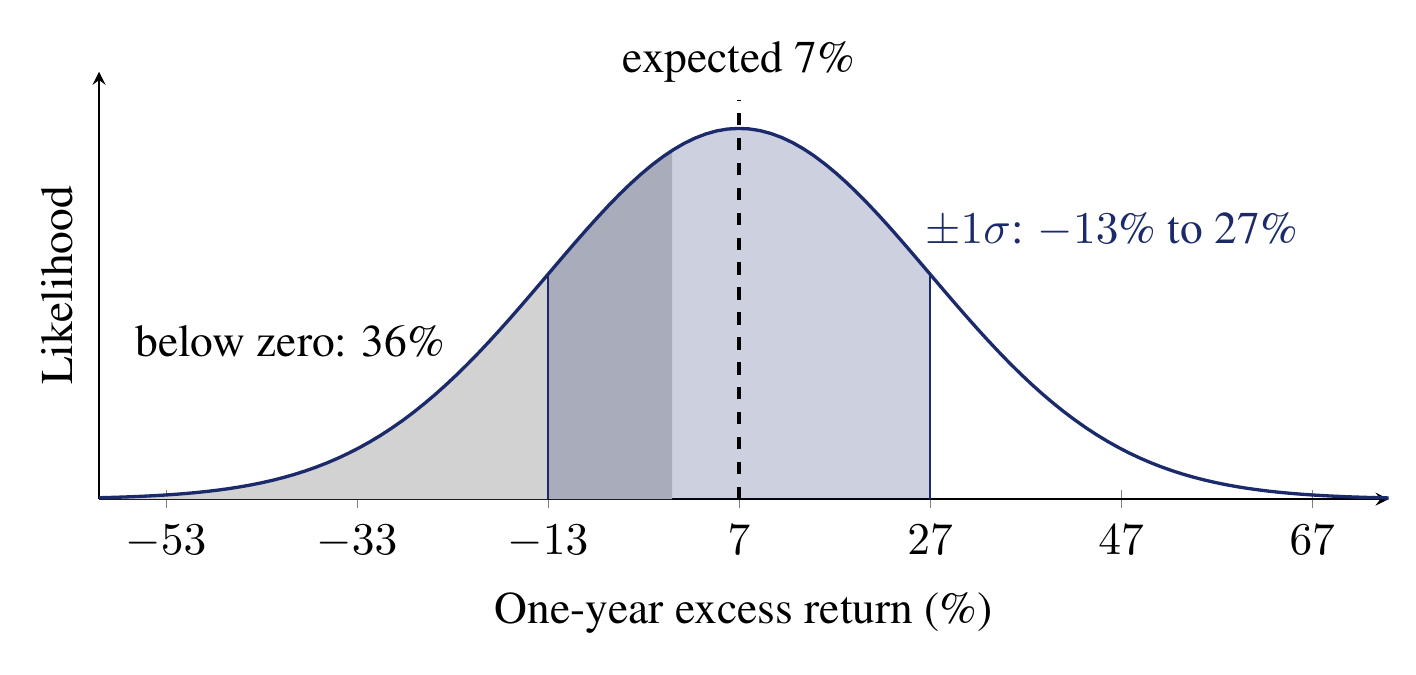
\includegraphics[width=0.85\linewidth]{images/fig01-1-one-year-return.png}
%\caption{One year's excess return on the stock market, assuming an expected excess return of 7\% and volatility of 20\%. The blue band covers the middle two-thirds of years, from $-13$\% to 27\%; the gray area is the 36\% of years with a negative excess return.}
%\label{fig:01-oneyear}
%\end{figure}


\subsection{The Sharpe ratio}
\label{sec:01-sharpe}

Sharpe (1966) proposed judging an investment by its excess return per unit of risk:
\begin{equation}
  \mathrm{SR} = \frac{E[R] - R_f}{\sigma} = \frac{E[R^{e}]}{\sigma}
  \label{eq:01-sr}
\end{equation}

The Sharpe ratio works much like a car's fuel economy. Miles per gallon tells you how far a car goes for each gallon it burns, and the Sharpe ratio tells you how much extra return an investment delivers for each unit of risk it carries. The stock market's long-run Sharpe ratio is around 0.3 to 0.4 a year. Because \term{leverage}\index{leverage} scales excess return and volatility equally, the Sharpe ratio does not change when a portfolio is levered up or down, which makes it the natural measure for comparing strategies (Figure~\ref{fig:01-sharpe-slope}).

%\begin{figure}[htbp]
%\centering
%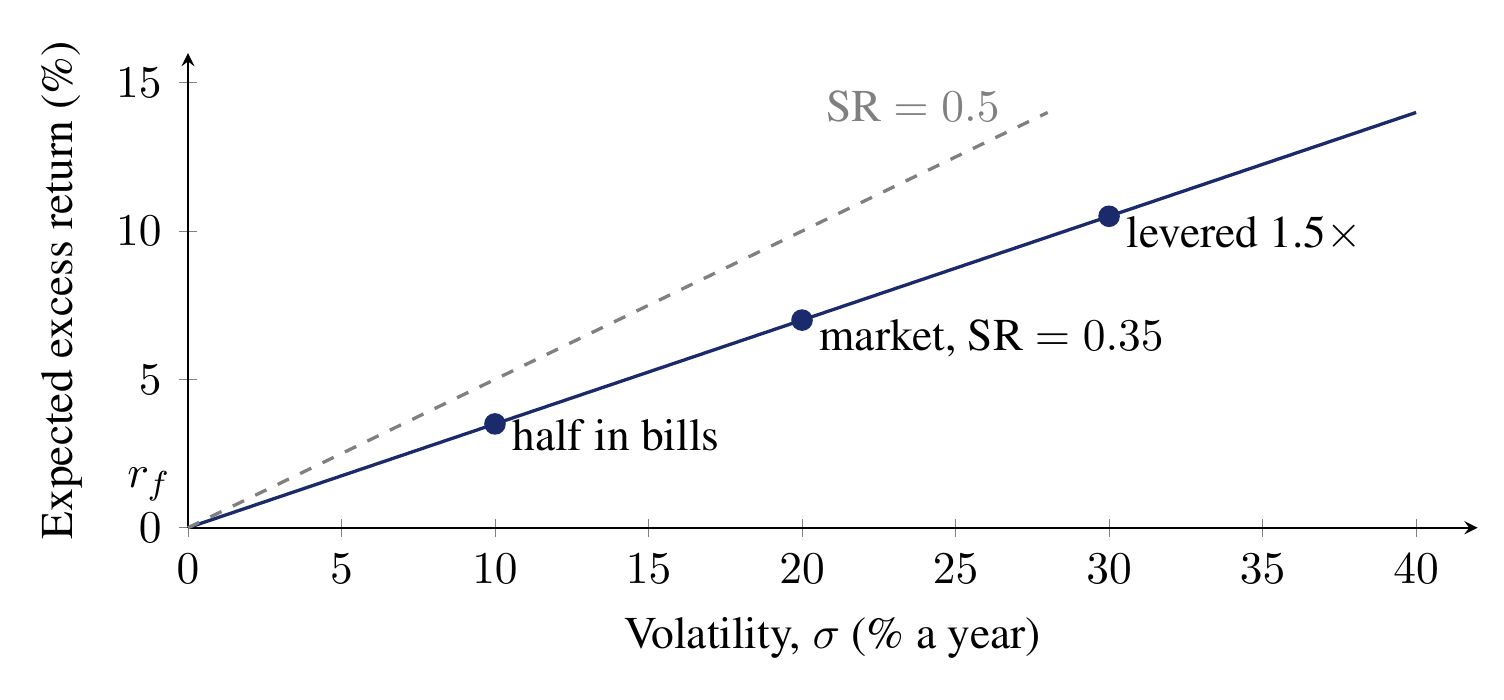
\includegraphics[width=0.85\linewidth]{images/fig01-2-sharpe-slope.png}
%\caption{The Sharpe ratio is the slope of a line from the risk-free rate. Leverage moves a portfolio along its line, raising or lowering both excess return and volatility, but does not change the slope. A better strategy lies on a steeper line.}
%\label{fig:01-sharpe-slope}
%\end{figure}

\providecolor{fenavy}{HTML}{1B2A6B}

\begin{figure}[!htbp]
  \centering
  \begin{tikzpicture}
  \begin{axis}[
    width=0.8\linewidth, height=0.42\linewidth,
    axis lines=left,
    axis line style={-stealth, thin},
    xmin=0, xmax=41, ymin=0, ymax=16,
    xtick={0,5,...,40},
    ytick={0,5,10,15},
    xlabel={Volatility, $\sigma$ (\% a year)},
    ylabel={Expected excess return (\%)},
    clip=false,
  ]
    % A higher Sharpe ratio, for comparison
    \addplot[gray, thick, dashed, domain=0:28, samples=2] {0.5*x};
    \node[gray, anchor=south] at (axis cs:23,14) {SR $= 0.5$};

    % Capital allocation line through the market (Sharpe ratio 0.35)
    \addplot[fenavy, thick, domain=0:40, samples=2] {0.35*x};

    % Portfolios on the line
    \fill[fenavy] (axis cs:10,3.5)  circle (2.6pt);
    \fill[fenavy] (axis cs:20,7)    circle (2.6pt);
    \fill[fenavy] (axis cs:30,10.5) circle (2.6pt);
    \node[anchor=north west, inner sep=2pt] at (axis cs:10.3,3.5) {half in bills};
    \node[anchor=north west, inner sep=2pt] at (axis cs:20.3,7)   {market, SR $= 0.35$};
    \node[anchor=north west, inner sep=2pt] at (axis cs:30.3,10.5) {levered $1.5\times$};

    % Risk-free asset at the origin
    \node[anchor=east] at (axis cs:-0.6,1.6) {$R_f$};
  \end{axis}
  \end{tikzpicture}
  \caption{Borrowing can make any strategy earn more, but only by taking more risk, so the fair comparison is return per unit of risk. The Sharpe ratio is the slope of a line from the risk-free rate. Leverage moves a portfolio along its line, raising or lowering both excess return and volatility, but does not change the slope. A better strategy lies on a steeper line.}
  \label{fig:01-sharpe-slope}
\end{figure}


\subsection{Risk, luck and skill}

Investors who make money in the stock market can do so for three different reasons. The distinction runs through the whole book.


\begin{itemize}
  \item \textbf{Bearing risk.} Stocks are riskier than Treasury bills, so over
  time they have paid more. This extra return is the equity premium defined
  above. An investor who simply buys and holds an index fund earns it without
  any special ability. Profit from bearing risk is a reward for risk, not
  evidence of skill.

  Here are three examples. (i) A retiree who has held an S\&P~500 index fund since
  1990 has earned far more than a savings account would have paid, without
  ever picking a stock. (ii) A manager who borrows to hold the index at
  1.5 times exposure, which means investing \$150 in stocks for every \$100
  of the fund's own money (a practice called leverage), beats the index in most years, but only because he
  carries 1.5 times its risk; in a crash he loses 1.5 times as much.
  (iii) A trader who sells \term{out-of-the-money}\index{option!moneyness} \term{put options}\index{option!put} collects a small,
  steady premium month after month and looks like a genius, until a market
  crash wipes out years of gains. A put option of this kind works like
  insurance against a market crash, so the trader is in effect an insurance
  company that collects premiums in calm years and pays out heavily when
  disaster strikes. In each case the extra return is payment
  for risk that anyone could have taken.

  \item \textbf{Luck.} Returns are noisy, so some investors do well by
  chance, sometimes for years at a time. We also hear more about the winners
  than the losers, which makes luck look more common than it is.

  Here are three examples. (i) Ten thousand people each flip a coin every year to
  decide whether to hold stocks or cash. After ten years, about ten of them
  will have called the market right every single year, and some will write
  books about their method. (ii) A newsletter sends 1{,}000 readers a
  ``buy'' call on a stock and another 1{,}000 a ``sell'' call. Whichever way
  the stock moves, half the readers now hold a correct prediction, and the
  trick can be repeated on that half. (iii) An investor puts her savings into
  one small biotech company just before it receives surprise drug approval.
  Her gain was real, but it rests on a single draw, so it says almost nothing
  about her ability.

  Real streaks raise the same question. Bill Miller's Legg Mason Value Trust
  beat the S\&P~500 in every calendar year from 1991 to 2005, a run of fifteen
  years that made him the most celebrated fund manager of his era. In 2008
  the fund lost about 55\% while the index fell about 38\%, and over his full
  tenure his average return ended up only slightly above the index's. A
  fifteen-year streak sounds impossible to achieve by chance, yet with
  thousands of funds competing, some long streaks are to be expected, and
  the streak alone cannot tell us how much was skill and how much was luck.


  \item \textbf{Skill.} Skill is the ability to earn more than the risk taken
  explains. It produces a return that a simple, cheap alternative carrying the
  same risk would not have delivered. Skill usually comes from better
  information, better analysis or better execution.

  Here are three examples, one of each kind. 
  With \textbf{(i) better
  information}, an analyst counts cars in retailers' parking lots from
  satellite images and forecasts sales before the companies report them.
  With \textbf{(ii) better analysis}, a fund beats a portfolio with the same
  market, \term{size and value exposures}, after fees, over twenty years and across
  many independent bets. Here ``size and value exposures'' means the fund is
  compared with a portfolio holding the same mix of small and large companies
  and of cheap and expensive stocks, so that its success cannot be explained
  by those well-known tilts alone (Chapter~\ref{ch:03}).
  With \textbf{(iii) better execution}, a trading firm
  buys and sells the same stocks as everyone else but pays less in \term{trading
  costs}\index{transaction costs} and \term{price impact}\index{market impact}. It keeps a few \term{basis points}\index{basis point} per trade that others
  give away. A basis point is one hundredth of a percentage point, so the
  saving on each trade is tiny, but it adds up over millions of trades.

  
  Researchers and practitioners have documented several cases that are widely
  regarded as genuine skill, and they fall into the same three groups.
  
  \begin{enumerate}
    \item \textbf{Better information.} The parking-lot example is not hypothetical.
  Satellite counts of retailers' parking lots are now sold to investors
  willing to pay for them, and Katona, Painter, Patatoukas and Zeng (2025)
  asked whether the data give their buyers a real edge. They found that
  buyers were able to trade profitably ahead of \term{earnings announcements},
  especially when the news was bad. Information that travels privately is
  harder to observe, so Cohen, Frazzini and Malloy (2008) traced the school
  ties between fund managers and executives. Managers earned higher returns
  on stocks of companies whose senior officers had attended the same
  university as the manager, which suggests that information can travel
  through personal networks. Many \term{insider trades} are routine and blur the
  signal in the rest, so Cohen, Malloy and Pomorski (2012) separated
  corporate insiders who trade on a regular schedule from those who break
  their routine. The routine trades carried little information, while the
  unusual trades predicted future returns.

    \item \textbf{Better analysis.} When thousands of funds compete, the best
  records may be luck, and fund returns have too many extreme months for the
  usual tests. Kosowski, Timmermann, Wermers and White (2006) addressed both
  problems with a \term{bootstrap}\index{bootstrap}, asking whether the best mutual
  fund records could be produced by luck alone. A bootstrap reshuffles a fund's actual monthly
  results many times to see how good the best records would look if no
  manager had any skill. They concluded that a minority of managers appear
  to pick stocks well enough to cover their costs, and that their records are
  difficult to explain by chance. Berk and van Binsbergen (2015) noted that
  investors pour money into a skilled manager's fund until its percentage
  return after fees looks ordinary, so they measured skill as the dollars a
  fund adds rather than as a percentage return. By
  that measure, the typical manager adds value, and differences in skill
  persist for many years. Kacperczyk, Sialm and Zheng (2005) asked why a
  professional would ignore the textbook advice to diversify, and found that
  funds concentrating on a few industries tend to outperform after adjusting for
  risk, consistent with managers who specialize in areas they understand well.

    \item \textbf{Better execution.} Academic studies often conclude that
  famous strategies lose their profits after trading costs, but they estimate
  those costs from models rather than from real institutional trades.
  Frazzini, Israel and Moskowitz (2018) studied the actual trades of a large
  asset manager and found that its trading costs were much lower than the
  estimates used in many academic studies. Careful
  execution can therefore turn a strategy that looks unprofitable on paper
  into one that works in practice. Speed is the extreme form of this
  skill, and Baron, Brogaard, Hagstr\"om{}er and Kirilenko (2019) studied the
  race among \term{high-frequency trading} firms. They found large and persistent
  differences in performance among these firms, which use computers to buy and sell
  within fractions of a second, and much of the difference was
  explained by how fast each firm could trade.
  
  \end{enumerate}

  Within the industry, the most frequently cited example is the Medallion
  Fund of Renaissance Technologies, whose exceptionally strong record over
  several decades is difficult to attribute to luck or to ordinary risk
  (Zuckerman, 2019). It is worth keeping these examples in proportion,
  however. Fama and French (2010) found that, after fees, very few mutual
  funds show evidence of skill, even though some do before fees. Genuine
  skill appears to exist, but it seems to be rare, and much of its value is
  often captured by the managers rather than passed on to investors.
  
  
\end{itemize}




\begin{callout}
\textbf{What Failed: Long-Term Capital Management.} 

In 1994 John Meriwether, a star bond trader, founded a \term{hedge fund}, a lightly regulated investment fund for wealthy investors and institutions that is free to borrow heavily and bet on falling as well as rising prices. Its partners included Myron Scholes and Robert Merton, who would share the 1997 Nobel Prize in economics. The fund bet that small price gaps between closely related bonds would close, and it borrowed heavily to turn those small gaps into large profits. For several years the record looked like proof of skill, with returns of roughly 40\% a year after fees in 1995 and 1996. 

In 1998, after Russia defaulted on its debt, investors everywhere fled to the safest assets, the gaps widened instead of closing, and the fund lost about \$4.6 billion in a few months. The Federal Reserve Bank of New York organized a rescue in which a group of banks put in \$3.6 billion to wind the fund down. Much of the fund's steady profit had been payment for bearing a rare crash risk, and a short record of good years could not reveal that risk until it struck (Lowenstein, 2000).
\end{callout}



\noindent\textbf{Which one is it?} Suppose an investor
consistently chooses the right stock at the right time. Before calling this
skill, ask two questions. First, \emph{does the risk explain it?} If the
investor's picks are mostly high-risk stocks bought during a rising market,
a cheap fund holding equally risky stocks might have done just as well, and
the profit is a reward for risk. Second, \emph{does luck explain it?} If the
record is short, or the investor is one of many whose picks we never hear
about, a run of good calls is what chance alone would produce. Only when the
answer to both questions is no does skill become the likely explanation. The
rest of this section shows how finance measures it.

\textbf{Finance measures skill with alpha}. The idea is simple even though the formula looks technical. We ask how much of a strategy's return could have been earned just by riding the market, and we call whatever is left over alpha. A regression is the statistical tool that does this split: it finds the straight line that best describes how the strategy's return moves with the market's. Regress a strategy's excess return on the market's excess return:
\begin{equation}
  R^{e}_{s} = \alpha + \beta\, R^{e}_{m} + \varepsilon \nonumber
\label{eq:ch01_beta}
\end{equation}
where $R^{e}_{s} = R_s - R_f$ is the strategy's excess return, $R^{e}_{m} = R_m - R_f$ is the market's excess return, as in Equation~\eqref{eq:excess-return}, and $\varepsilon$ is the part of the return the regression does not explain. The coefficient $\beta$ (\term{beta}\index{beta|textbf}) measures how much market risk the strategy carries. A fund with a beta of 1.5, for example, tends to rise about 15\% when the market rises 10\% and to fall about 15\% when the market falls 10\%. The term $\beta\, R^{e}_{m}$ is therefore the return that market exposure alone would have delivered. The intercept $\alpha$ is what is left over, that is, the average return beyond what the strategy's market risk explains. For example, suppose a strategy has a beta of 0.6 and earns an average excess return of 6\% a year while the market earns 8\%. Market risk explains $0.6 \times 8 = 4.8$\%, so the strategy's alpha is $6 - 4.8 = 1.2$\% a year. Chapter~\ref{ch:03} develops this regression and its extensions to other sources of risk.

A positive alpha is necessary for skill but not sufficient, because luck also produces positive alphas. Telling the two apart is the central problem of this chapter.

\subsection{Estimating a mean, and how uncertain the estimate is}
\label{sec:01-se}

An average computed from a limited number of years is only an estimate of the true average, and the \emph{standard error} tells us how far off that estimate is likely to be. Given $T$ independent observations of a return with standard deviation $\sigma$, the sample mean $\bar{R}$ has a \term{standard error}\index{standard error|textbf} of
\begin{equation}
  \mathrm{SE}(\bar{R}) = \frac{\sigma}{\sqrt{T}}.
  \label{eq:01-se}
\end{equation}
The standard error measures how far the sample mean is likely to fall from the true mean, and it shrinks only with the square root of the number of observations, so quadrupling the data merely halves it. The \term{t-statistic}\index{t-statistic|textbf} is a signal-to-noise ratio. It counts how many units of noise an average return sits above zero, and as a rule of thumb a value above about 2 means the result is unlikely to be luck. Formally, the t-statistic of a mean is the estimate divided by its standard error; under the hypothesis that the true mean is zero, it has approximately a standard \term{normal distribution}\index{distribution!normal}, so values beyond about $\pm 1.96$ occur by chance only 5\% of the time. Applied to the Sharpe ratio, the same arithmetic gives a useful rule: the t-statistic of a strategy's mean return is approximately its annual Sharpe ratio times the square root of the number of years. A Sharpe ratio of 0.5
needs about 15 years of data before the t-statistic of its mean return reaches 1.96 (Figure~\ref{fig:01-years}).

%\begin{figure}[htbp]
%\centering
%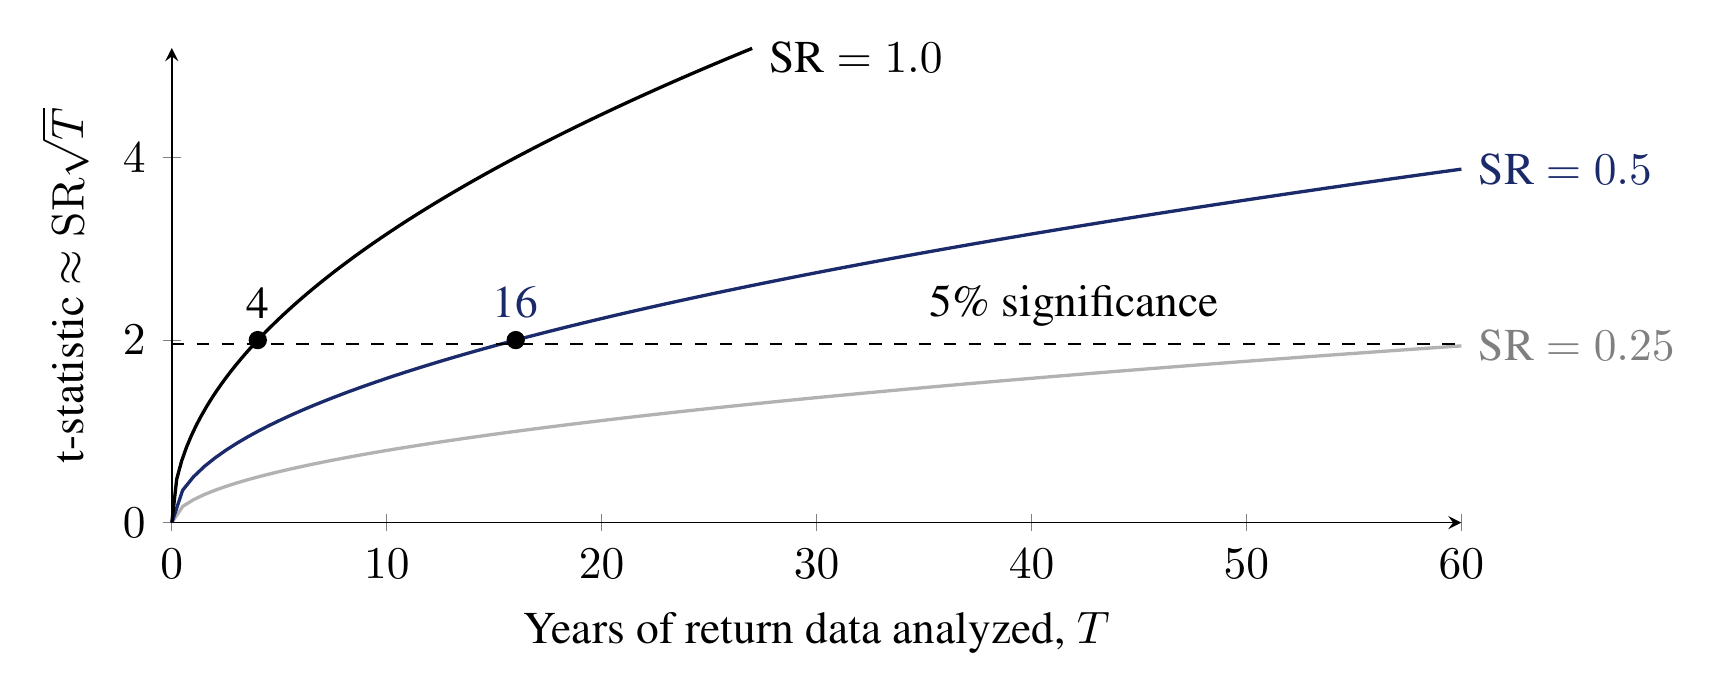
\includegraphics[width=0.85\linewidth]{images/fig01-3-years-needed.png}
%\caption{How many years of return data are needed before a strategy's track record becomes statistically significant. The years count the length of the history being analyzed, not how long the strategy must trade or hold its positions. With a true Sharpe ratio of 0.5, about 15 years of data are needed to reach $t = 1.96$; with 0.25, about 61.}
%\label{fig:01-years}
%\end{figure}


\providecolor{fenavy}{HTML}{1B2A6B}

\begin{figure}[!htbp]
  \centering
  \begin{tikzpicture}
  \begin{axis}[
    width=0.78\linewidth, height=0.4\linewidth,
    axis lines=left,
    axis line style={-stealth, thin},
    xmin=0, xmax=61, ymin=0, ymax=5.4,
    xtick={0,10,...,60},
    ytick={0,2,4},
    xlabel={Years of return data analyzed, $T$},
    ylabel={t-statistic $\approx \mathrm{SR}\sqrt{T}$},
    samples=200,
    clip=false,
  ]
    % 5% significance
    \addplot[thick, dashed, domain=0:60, samples=2] {2};
    \node[anchor=south] at (axis cs:40,2.05) {5\% significance};

    % t = SR * sqrt(T) for three Sharpe ratios
    \addplot[thick, black, domain=0:27] {1.0*sqrt(x)};
    \addplot[thick, fenavy, domain=0:60] {0.5*sqrt(x)};
    \addplot[thick, gray!55, domain=0:60] {0.25*sqrt(x)};

    \node[anchor=west] at (axis cs:28,{sqrt(27)}) {SR $= 1.0$};
    \node[fenavy, anchor=west] at (axis cs:60.5,{0.5*sqrt(60)}) {SR $= 0.5$};
    \node[gray, anchor=west] at (axis cs:60.5,{0.25*sqrt(60)}) {SR $= 0.25$};

    % Years needed to reach t = 2
    \fill (axis cs:4,2)  circle (2.4pt);
    \fill (axis cs:16,2) circle (2.4pt);
    \node[anchor=south] at (axis cs:4,2.08) {4};
    \node[fenavy, anchor=south] at (axis cs:16,2.08) {16};
  \end{axis}
  \end{tikzpicture}
  \caption{The weaker a strategy's edge, the longer its record must be before luck can be ruled out. The curves show how many years of return data are needed before a strategy's track record becomes statistically significant. The years count the length of the history being analyzed, not how long the strategy must trade or hold its positions. With a true Sharpe ratio of 0.5, about 15 years of data are needed to reach $t = 1.96$. With a Sharpe ratio of 0.25, about 61 years are needed.}
  \label{fig:01-years}
\end{figure}



\textbf{Worked example.} A strategy earns an average excess return of 0.5\% a month with a monthly standard deviation of 4\% over 10 years. Its annual mean is 6\%, its annual volatility is 4\% $\times \sqrt{12} \approx 13.9$\%, and its Sharpe ratio is $6/13.9 \approx 0.43$. The t-statistic is $0.5 / (4/\sqrt{120}) \approx 1.37$. This is not \term{statistically significant} at the 5\% level, even though the strategy may be genuinely good.



\section{Efficient markets and the random walk}
\label{sec:01-efficient-markets}

The starting point for any claim about beating the market is the \term{efficient market hypothesis}. In Eugene Fama's (1970) formulation, a market is efficient if prices fully reflect available information. The intuition comes from competition. If a predictable profit existed, traders would act on it, and their trading would push prices until the profit disappeared.

Fama distinguished three versions by the information set\index{forecasting!information set}:

\begingroup
\small
\setlength{\LTpre}{6pt}\setlength{\LTpost}{6pt}
\begin{longtable}{@{}>{\raggedright\arraybackslash}p{0.180\linewidth}>{\raggedright\arraybackslash}p{0.234\linewidth}>{\raggedright\arraybackslash}p{\dimexpr 0.9\linewidth-0.180\linewidth-0.234\linewidth-4\tabcolsep\relax}@{}}
\toprule
Version & Prices reflect & Implication if true \\
\midrule
\endfirsthead
\multicolumn{3}{@{}l}{\emph{(continued)}} \\
\toprule
Version & Prices reflect & Implication if true \\
\midrule
\endhead
\midrule
\multicolumn{3}{r@{}}{\emph{(continued on the next page)}} \\
\endfoot
\bottomrule
\endlastfoot
\term{Weak form} & Past prices and trading volume & Technical trading rules cannot earn abnormal returns \\*
\term{Semi-strong form} & All public information & Analysis of public news and accounting data cannot earn abnormal returns \\*
\term{Strong form} & All information, including private & Even insiders cannot earn abnormal returns \\*
\end{longtable}
\addtocounter{table}{-1}% uncaptioned longtable: keep table numbers unchanged
\endgroup

An \term{abnormal return} in the table means a return above what the investment's risk would justify, which is the alpha of Section~\ref{sec:01-foundations}. Everyday examples make the three versions concrete. A trader who studies price charts to spot patterns is betting against the weak form. An investor who reads company earnings reports and news stories to pick stocks is betting against the semi-strong form. A company executive who buys shares before a merger is announced, using news the public does not yet have, is betting against the strong form, and in most countries that trade is illegal insider trading.

Few economists believe the strong form\index{efficient market hypothesis!strong form}, and insider-trading laws exist because it fails. The weak and semi-strong forms are where the empirical debate happens, and where most claims in this book live.

\textbf{What efficiency does not imply.} Efficiency is often misread, so three clarifications matter:

\begin{enumerate}
  \item \textbf{It does not mean returns are unpredictable in every sense.} Expected returns can vary over time or across stocks as compensation for risk. A predictable return that is fair payment for risk is consistent with efficiency, but a predictable return that is a free lunch is not. Separating the two is known as the \term{joint-hypothesis problem}\index{joint-hypothesis problem}, because every test of efficiency is also a test of a model of what returns \emph{should} be.
  \item \textbf{It does not mean prices are always right.} It means mispricings are hard to identify and profit from after costs. Grossman and Stiglitz (1980) showed that a perfectly efficient market is impossible, because if prices reflected everything, no one would pay to gather information. Markets must be inefficient enough to reward the people who make them efficient. An old joke captures the tension. An economist walking with a friend refuses to pick up a \$20 bill lying on the sidewalk, explaining that if it were real, someone would already have taken it. Grossman and Stiglitz's point is that someone must keep looking for \$20 bills, and that a few can be found by those who search hardest.
  \item \textbf{It does not mean volatility is unpredictable.} As Chapter~\ref{ch:07} shows, risk is far more predictable than return.
\end{enumerate}

\textbf{The random walk\index{random walk} as a benchmark.} If prices respond only to new, unpredictable information, price changes should look approximately like a random walk, in which tomorrow's change is unrelated to today's. Samuelson (1965) showed that properly anticipated prices fluctuate randomly. In plain words, if today's price already reflects everything investors expect, then only surprises can move it, and surprises by definition cannot be predicted from today's price change. Lo and MacKinlay (1988) later rejected a strict random walk for weekly U.S. returns, finding small but measurable patterns from one week to the next, so the model is not literally true. Even so, it remains the right benchmark, and any strategy must beat what a random walk, or a simple buy-and-hold position, would deliver.

For this book, the practical lesson is a prior belief that we bring to every claim. Before seeing any evidence, we should treat a claim that a simple rule beats the market as unlikely. Such a claim is not impossible, since the following chapters find some rules that survive, but it is unlikely enough to demand strong evidence.

\section{Signal and noise}
\label{sec:01-signal-noise}

The deeper reason claims are hard to verify is statistical. In finance, the signal is small and the noise is large. The differences between good and bad strategies are a few percent a year in expected return, while their returns move by fifteen or twenty percent a year at random.

\textbf{The Sharpe ratio, again.}\index{Sharpe ratio|textbf} The yardstick for a strategy is the Sharpe ratio of Equation~\eqref{eq:01-sr}. In this section we write $\mu = E[R^{e}]$ for the strategy's expected excess return, so that $\mathrm{SR} = \mu/\sigma$, with all quantities annualized. The rest of the book uses $\mu$ in the same way. Against the stock market's long-run Sharpe ratio of 0.3 to 0.4 (Section~\ref{sec:01-foundations}), a strategy with a true Sharpe ratio of 0.5 after costs would be a valuable discovery, and 1.0 would be exceptional.

\textbf{How precisely can we measure it?} With $T$ years of independent returns, the t-statistic for testing whether the true Sharpe ratio is zero is approximately
\begin{equation}
  t \approx \mathrm{SR}\,\sqrt{T}
  \label{eq:01-t}
\end{equation}
In words, the evidence for a strategy grows only with the square root of the length of its record, so a record must be four times as long to make the evidence twice as strong. The shaded box shows where the formula comes from.

\begin{technote}
\textbf{Technical note: where the rule comes from.} Equation~\eqref{eq:01-t} follows from the definition of the Sharpe ratio in Equation~\eqref{eq:01-sr} in four steps.

\begin{enumerate}
  \item \textbf{Estimate the mean.} Take $T$ years of annual excess returns. Their sample average, $\bar{R}^{e}$, is our estimate of the expected excess return $\mu$.
  \item \textbf{Find its standard error.} If the yearly returns are independent with volatility $\sigma$, the standard error of an average of $T$ of them is
  \begin{equation}
    \mathrm{SE}(\bar{R}^{e}) = \frac{\sigma}{\sqrt{T}} \nonumber
  \end{equation}
  \item \textbf{Form the t-statistic.} To test whether the true mean is zero, divide the estimate by its standard error:
  \begin{equation}
    t = \frac{\bar{R}^{e}}{\sigma/\sqrt{T}} = \frac{\bar{R}^{e}}{\sigma}\,\sqrt{T} \nonumber
  \end{equation}
  \item \textbf{Recognize the Sharpe ratio.} The ratio $\bar{R}^{e}/\sigma$ is the measured Sharpe ratio. Replacing $\bar{R}^{e}$ with the true mean $\mu$ gives the t-statistic we should expect on average:
  \begin{equation}
    t \approx \frac{\mu}{\sigma}\,\sqrt{T} = \mathrm{SR}\,\sqrt{T} \nonumber
  \end{equation}
  The result is approximate for two reasons: the measured mean differs from the true one, and in practice $\sigma$ must be estimated as well.
\end{enumerate}

The answer is the same with monthly or daily data. Sampling $k$ times a year gives $kT$ observations, each with mean $\mu/k$ and volatility $\sigma/\sqrt{k}$, so
\begin{equation}
  t = \frac{\mu/k}{(\sigma/\sqrt{k})/\sqrt{kT}} = \frac{\mu}{\sigma}\,\sqrt{T} \nonumber
\end{equation}
and the sampling frequency $k$ cancels.
\end{technote}

By the same reasoning, the standard error of an estimated annual Sharpe ratio is roughly $1/\sqrt{T}$. Lo (2002) gives the refinements for non-normal and autocorrelated returns, but the rough version is enough to see the problem. Setting $t = 1.96$, the usual 5\% significance threshold, in Equation~\eqref{eq:01-t} and solving for $T$ gives the number of years needed before a strategy's record can be distinguished from luck. Dividing both sides by SR gives $\sqrt{T} \approx 1.96/\mathrm{SR}$, and squaring gives
\begin{equation}
  T \approx \left(\frac{1.96}{\mathrm{SR}}\right)^2
  \label{eq:01-T}
\end{equation}

\begingroup
\small
\setlength{\LTpre}{6pt}\setlength{\LTpost}{6pt}
\begin{longtable}{@{}ll@{}}
\toprule
True Sharpe ratio & Years of data needed for the mean return to reach $t = 1.96$ \\
\midrule
\endfirsthead
\multicolumn{2}{@{}l}{\emph{(continued)}} \\
\toprule
True Sharpe ratio & Years of data needed for the mean return to reach $t = 1.96$ \\
\midrule
\endhead
\midrule
\multicolumn{2}{r@{}}{\emph{(continued on the next page)}} \\
\endfoot
\bottomrule
\endlastfoot
0.25 & 61 \\*
0.50 & 15 \\
0.75 & 7 \\
1.00 & 4 \\*
1.50 & 2 \\
\end{longtable}
\addtocounter{table}{-1}% uncaptioned longtable: keep table numbers unchanged
\endgroup

A strategy as good as the stock market itself needs more than two decades of data before its record is statistically convincing. Most fund track records, and most backtests shown to investors, are far shorter.

A natural question is whether daily data could shorten the wait, since a decade contains about 2,500 trading days but only 120 months. They cannot. The precision of an average return depends on the number of years in the record, not on how often returns are written down, although frequent data do help when the goal is to measure risk. The shaded box explains why.

\begingroup
\small
\setlength{\LTpre}{6pt}\setlength{\LTpost}{6pt}
\begin{longtable}{@{}lrrrrrr@{}}
\caption{The same 16-year record measured annually, monthly and daily. The expected excess return is 10\% a year and the volatility is 20\% a year, so the annual Sharpe ratio is 0.5. The daily figures assume 252 trading days a year.}
\label{tab:01-frequency} \\
\toprule
Frequency & Observations & Mean per & Volatility per & Sharpe ratio & $\sqrt{N}$ & $t$ \\
 & $N$ & period (\%) & period (\%) & per period & & \\
\midrule
\endfirsthead
\multicolumn{7}{@{}l}{\emph{(continued)}} \\
\toprule
Frequency & Observations & Mean per & Volatility per & Sharpe ratio & $\sqrt{N}$ & $t$ \\
 & $N$ & period (\%) & period (\%) & per period & & \\
\midrule
\endhead
\midrule
\multicolumn{7}{r@{}}{\emph{(continued on the next page)}} \\
\endfoot
\bottomrule
\endlastfoot
Annual  & 16    & 10.000 & 20.00 & 0.500  & 4.00  & 2.00 \\*
Monthly & 192   & 0.833  & 5.77  & 0.144  & 13.86 & 2.00 \\*
Daily   & 4{,}032 & 0.040 & 1.26  & 0.0315 & 63.50 & 2.00 \\*
\end{longtable}
\endgroup

\begin{technote}
\textbf{Technical note: does the return frequency matter?} For the years-needed table above, it does not. Daily data give 252 observations a year instead of 12, but each daily return carries proportionally less information about the mean, so the years needed are the same. Table~\ref{tab:01-frequency} shows this for one strategy observed over the same 16 years at three frequencies. The strategy has an expected excess return of 10\% a year and a volatility of 20\%, so its Sharpe ratio is 0.5. The t-statistic is always the Sharpe ratio \emph{per period} times the square root of the \emph{number of periods}. Sampling more often multiplies the number of observations, but shrinks the Sharpe ratio of each one by the square root of that factor, and the two effects cancel.


Going from annual to monthly data gives 12 times as many observations, but each has a mean 12 times smaller and a volatility $\sqrt{12}$ times smaller, so its Sharpe ratio is $\sqrt{12}$ times smaller. Since $\sqrt{N}$ grows by exactly $\sqrt{12}$, the t-statistic does not change. The same happens with 252 in place of 12 for daily data. This is why Equation~\eqref{eq:01-t} can be stated in years. $T$ counts observations only when the Sharpe ratio is measured over the same period, and for an annual Sharpe ratio that period is a year. Merton (1980) made the general point that the precision of an estimated expected return depends on the length of the history, not on the sampling frequency. With log returns the reason is especially plain. The average annual log return over $T$ years depends only on the first and last prices,
\begin{equation}
  \bar{r} = \frac{\ln P_T - \ln P_0}{T}, \nonumber
\end{equation}
because every price in between is added once and subtracted once. Dividing a century into days rather than months adds no information about the mean, and its standard error stays at about $20/\sqrt{100} = 2$\%, as in Section~\ref{sec:01-foundations}. The same holds for every claim about \emph{average} returns, such as the equity premium, value, momentum\index{momentum} and published anomalies\index{anomaly}, which is why Chapters~\ref{ch:03} to~\ref{ch:15} can test them on monthly data without losing anything.

Claims about \emph{risk} are different. Each additional observation adds information about how much returns vary, so the precision of an estimated volatility grows with the number of returns $N$, not just the number of years:
\begin{equation}
  \mathrm{SE}(\hat{\sigma}) \approx \frac{\sigma}{\sqrt{2N}} \nonumber
\end{equation}
With 20\% volatility and a century of data, the standard error is about 0.41 percentage points with monthly returns ($N = 1{,}200$) and about 0.09 with daily returns ($N \approx 25{,}200$), more than four times smaller. This is why the chapters on volatility (Chapter~\ref{ch:07}), value at risk\index{Value at Risk (VaR)} (Chapter~\ref{ch:08}), trading costs (Chapter~\ref{ch:13}) and delta hedging\index{delta hedging} (Chapter~\ref{ch:17}) use daily or even intraday data.

The rule ``the mean needs a long history, risk needs frequent data'' is a good guide, but it has limits.
\begin{itemize}
  \item \textbf{Very high frequency adds noise.} At intraday frequencies, the bounce between \term{bid and ask prices} (the prices at which dealers will buy and sell) and stale quotes distort measured returns, so for volatility, more frequent data help only up to a point.
  \item \textbf{Daily betas can be biased.} Stocks that trade infrequently react to market news with a delay, which makes their daily betas too low. Monthly data, or a correction that adds lagged market returns to the regression (Dimson, 1979), reduces the bias. This matters for the low-risk anomaly\index{low-risk anomaly} in Chapter~\ref{ch:14}.
  \item \textbf{Annualizing is not automatic.} The rules in Section~\ref{sec:01-foundations} for converting monthly figures to annual ones assume that returns are uncorrelated over time. When they are \term{autocorrelated}, meaning that one month's return partly echoes the last, as for many hedge funds and illiquid assets that trade rarely and are hard to price, a monthly Sharpe ratio multiplied by $\sqrt{12}$ can be badly off (Lo, 2002).
  \item \textbf{The cancellation is exact only for log returns.} For simple returns, the precision of the mean still depends mainly on the length of the history, but only approximately.
\end{itemize}
\end{technote}

The practical lesson is to match the data to the claim. To measure an expected return more precisely, you need a longer history, not more frequent data. To measure risk, more frequent data do help.

\textbf{What a ten-year record can tell you.} The ``10 years'' here is not how long the strategy holds its positions, since the strategy may trade daily or monthly. It is the length of the track record you look at when you judge the strategy. A thought experiment shows how noisy that judgment is.

\begin{enumerate}
  \item \textbf{The strategy is genuinely good.} Suppose its true Sharpe ratio is 0.5. Nobody can see this number directly. We see only the Sharpe ratio measured from its \term{realized returns}\index{return!realized}.
  \item \textbf{The measurement is noisy.} With a 10-year record, the standard error of the measured Sharpe ratio is about $1/\sqrt{10} \approx 0.32$.
  \item \textbf{The record could show almost anything.} A 95\% range for the measured Sharpe ratio is $0.5 \pm 1.96 \times 0.32$, or about $-0.1$ to 1.1. Imagine watching the same strategy over many different decades. In one decade it looks like a star, with a Sharpe ratio near 1.0. In another it looks like a failure, with a Sharpe ratio near zero. The strategy is the same, and only the decade differs.
  \item \textbf{Luck can look like skill.} A strategy with no skill has a true Sharpe ratio of zero, yet its measured Sharpe ratio exceeds 0.5 whenever the noise is more than $0.5/0.32 \approx 1.6$ standard errors. That happens in roughly 6\% of decades, by luck alone.
\end{enumerate}

Figure~\ref{fig:01-ten-year} draws the two cases side by side. The curves overlap heavily. A measured Sharpe ratio of 0.4, for example, is quite consistent with both a genuinely good strategy and a useless one. A ten-year record cannot reliably tell them apart.

\providecolor{fenavy}{HTML}{1B2A6B}
\providecolor{fegray}{HTML}{4D4D4D}

\begin{figure}[!htbp]
  \centering
  \begin{tikzpicture}[
    % Estimated Sharpe ratio from a 10-year record: s.e. = 1/sqrt(10)
    declare function={
      se = 1/sqrt(10);
      npdf(\x,\m) = exp(-0.5*((\x-\m)/se)^2)/(se*sqrt(2*pi));
    }]
  \begin{axis}[
    scale only axis, width=0.7\linewidth, height=0.3\linewidth,
    axis lines=left,
    axis line style={-stealth, thin},
    xmin=-1.25, xmax=1.8, ymin=0, ymax=1.6,
    xtick={-1,-0.5,0,0.5,1,1.5},
    xticklabel style={/pgf/number format/fixed},
    ytick=\empty,
    ylabel={Likelihood},
    xlabel={Sharpe ratio measured from a 10-year record},
    xlabel style={yshift=-28pt},
    samples=200,
    clip=false,
  ]
    % No skill: true SR = 0
    \addplot[name path=null, fegray, thick, domain=-1.25:1.6] {npdf(x,0)};
    \path[name path=base] (axis cs:-1.25,0) -- (axis cs:1.8,0);
    % No-skill records above 0.5
    \addplot[fill=gray!40, draw=none]
      fill between[of=null and base, soft clip={domain=0.5:1.6}];

    % Good strategy: true SR = 0.5
    \addplot[fenavy, thick, domain=-0.75:1.8] {npdf(x,0.5)};

    % Centers
    \draw[fegray, dashed] (axis cs:0,0) -- (axis cs:0,{npdf(0,0)});
    \draw[fenavy, dashed] (axis cs:0.5,0) -- (axis cs:0.5,{npdf(0.5,0.5)});
    \node[fegray, anchor=south east, align=center] at (axis cs:0.05,1.3)
      {no skill\\(true SR $= 0$)};
    \node[fenavy, anchor=south west, align=center] at (axis cs:0.45,1.3)
      {good strategy\\(true SR $= 0.5$)};

    % Share of no-skill records above 0.5
    \node[fegray, anchor=south west, align=left] at (axis cs:1.12,0.62)
      {no-skill records\\above 0.5: about 6\%};
    \draw[-stealth, gray] (axis cs:1.2,0.6) -- (axis cs:0.78,0.17);

    % 95% range of the good strategy's measured Sharpe ratio
    \draw[fenavy, thick, |<->|] (axis cs:-0.12,-0.33) -- (axis cs:1.12,-0.33);
    \node[fenavy, anchor=north] at (axis cs:0.5,-0.36)
      {95\% of decades: $-0.1$ to $1.1$};
  \end{axis}
  \end{tikzpicture}
  \caption{What a 10-year record can show. Even a decade of results cannot reliably tell a good strategy from a useless one, because the two ranges of outcomes overlap heavily. The gray curve is the range of Sharpe ratios a strategy with no skill produces over different decades, and the blue curve is the same for a strategy with a true Sharpe ratio of 0.5. The shaded tail is the 6\% of decades in which the useless strategy beats 0.5 by luck.}
  \label{fig:01-ten-year}
\end{figure}


%\begin{figure}[htbp]
%\centering
%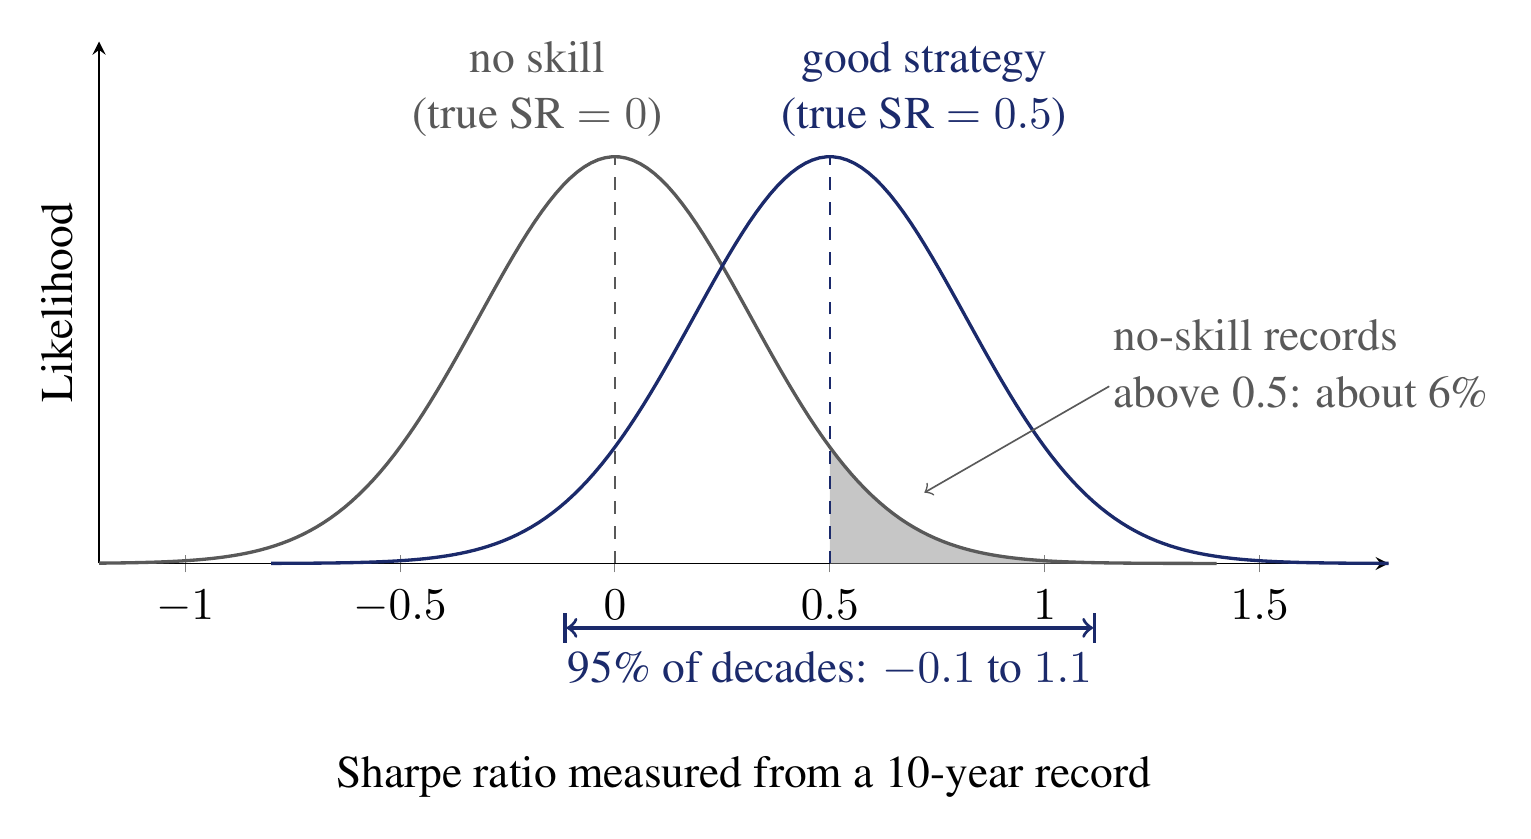
\includegraphics[width=0.85\linewidth]{images/fig01-4-ten-year-record.png}
%\caption{What a 10-year record can show. The gray curve is the range of Sharpe ratios a strategy with no skill produces over different decades; the blue curve is the same for a strategy with a true Sharpe ratio of 0.5. The shaded tail is the 6\% of decades in which the useless strategy beats 0.5 by luck.}
%\label{fig:01-ten-year}
%\end{figure}

\textbf{Why prediction is harder than it looks.} The same arithmetic applies to forecasting. A model that explains just 1\% of the variation in monthly returns would be worth a great deal to an investor (Campbell and Thompson 2008 make this point). The share of variation a model explains is called its \term{$R^2$}\index{regression!R-squared@$R^2$}. An $R^2$ of 1\% is almost impossible to distinguish from zero in a few decades of data, and almost trivially easy to produce by accident when many models are tried. Small true effects, large noise and short samples together make finance a field where false discoveries are easy and true ones are hard to confirm.

\section{Cautions: Why backtests can mislead}
\label{sec:01-backtests}

A backtest applies a strategy's rules to historical data to show how it would have performed. It is the most common evidence offered for a strategy and the easiest to get wrong. Seven problems account for most misleading backtests; later chapters treat each in depth.

\begin{enumerate}
  \item \textbf{Selection across many trials.} If you test 100 rules and report the best, its record overstates what it will deliver. It is like the Texas sharpshooter who fires at the side of a barn and then paints a target around the tightest cluster of bullet holes. This is the subject of the lab, and Chapter~\ref{ch:15} returns to it.
  \item \textbf{Overfitting parameters.}\index{overfitting|textbf} Tuning a rule's settings, such as choosing a 47-day average instead of 50 or a threshold of 1.3 instead of 1.5, fits the noise in the sample. The result is like a suit tailored to a single pose, which fits perfectly in that pose and badly in every other. Each added parameter is another hidden trial.
  \item \textbf{Look-ahead bias.}\index{look-ahead bias|textbf} A backtest may use information that was not available at the time, such as revised economic data, or accounting figures before their release date (Chapter~\ref{ch:02}). It is the backtesting equivalent of betting on a game after you already know the final score.
  \item \textbf{Survivorship bias.}\index{survivorship bias|textbf} A backtest may test only companies or funds that still exist, which leaves out the ones that failed (Chapter~\ref{ch:02}). During the Second World War, the statistician Abraham Wald made the same point about bombers: studying the bullet holes on planes that came home would put armor in the wrong places, because the planes hit in the most vulnerable spots never returned.
  \item \textbf{Ignoring costs.} Spreads, commissions, market impact, borrowing fees\index{borrowing fee} and taxes\index{taxes} can erase a paper profit, especially for high-turnover\index{turnover} strategies (Chapter~\ref{ch:13}).
  \item \textbf{Short or unrepresentative samples.} A decade of data may contain only one market regime, such as a long boom with no crash, so it says little about how the strategy would fare when conditions change. As Section~\ref{sec:01-signal-noise} showed, a short sample cannot separate skill from luck.
  \item \textbf{A story told after the fact.} Once a pattern is found, a plausible explanation is easy to write. The story makes the result feel robust, but it was written to fit the data, not tested against it.
\end{enumerate}

These problems compound. A backtest can be honest in every visible detail, using correct prices, real costs and no look-ahead, and still mislead because it is the best of many attempts that are never shown.

\begin{callout}
\textbf{What Failed: butter in Bangladesh.} To show how easy \term{data mining}\index{data mining} is, David Leinweber searched a United Nations database for series that tracked the S\&P 500. Butter production in Bangladesh fit well. Adding U.S. cheese production and the sheep population of Bangladesh and the United States raised the fit further, until the $R^2$ looked like a breakthrough. The relationship, of course, predicted nothing afterward. The example was a joke with a serious point: if you search enough series, you are guaranteed to find a near-perfect fit. Leinweber later wrote it up as ``Stupid Data Miner Tricks'' (2007).
\end{callout}

\section{The claims-on-trial method and the verdict scale}
\label{sec:01-method}

Every claim chapter and every lab opens with a line labelled \textbf{Claim on trial}\index{claims-on-trial method|textbf}. The label is a reminder of who does the work. You are not told whether the claim is true; you test it yourself. The book's subtitle, \emph{Active Learning by Verifying Famous Claims}, describes the bargain. Each trial needs a method (a regression, a backtest, a volatility model, a hedge), and you learn that method in order to reach a verdict, then use it again in later trials until it is second nature.

The rest of this book applies one method to every claim. It is simple enough to remember and strict enough to protect against the problems in Section~\ref{sec:01-backtests}.

\begin{enumerate}
  \item \textbf{Claim} --- State what is asserted in one testable sentence. ``Momentum works'' is vague; ``stocks with the highest 12-month returns, skipping the last month, outperform the lowest by a positive average return after costs'' can be tested.
  \item \textbf{Understand} --- Learn how the idea works and how the original evidence was produced, including the data, the sample period, the method and the number of alternatives the authors tried.
  \item \textbf{Verify} --- Rebuild the result yourself, then stress-test it \term{out of sample}\index{in-sample versus out-of-sample}, in other markets, after costs and after publication.
  \item \textbf{Judge} --- Compare your results with the published evidence, which each chapter summarizes in a section called \emph{Where the evidence stands}. Then reach your own verdict on the scale below, and date it with the sample period you tested.
  \item \textbf{Apply} --- State what an investor or practitioner can actually use, and what remains open.
\end{enumerate}

\textbf{The verdict scale}\index{verdict scale|textbf}

\begingroup
\small
\setlength{\LTpre}{6pt}\setlength{\LTpost}{6pt}
\begin{longtable}{@{}>{\raggedright\arraybackslash}p{0.162\linewidth}>{\raggedright\arraybackslash}p{\dimexpr 0.9\linewidth-0.162\linewidth-2\tabcolsep\relax}@{}}
\toprule
Verdict & Meaning \\
\midrule
\endfirsthead
\multicolumn{2}{@{}l}{\emph{(continued)}} \\
\toprule
Verdict & Meaning \\
\midrule
\endhead
\midrule
\multicolumn{2}{r@{}}{\emph{(continued on the next page)}} \\
\endfoot
\bottomrule
\endlastfoot
Survives & The result replicates, holds out of sample and in other markets, and remains economically meaningful after costs. \\*
Weakens & The result is real but smaller, less reliable, or narrower than claimed, for example only in small stocks or before publication. \\
Fails & The result does not replicate, or disappears out of sample or after costs. \\*
Provisional & The evidence is too new or too mixed for a firm verdict. \\
\end{longtable}
\addtocounter{table}{-1}% uncaptioned longtable: keep table numbers unchanged
\endgroup

Two habits make the method work. First, \textbf{decide the test before seeing the result}. Write down the claim, the data and the pass criteria in advance, so that the test cannot be bent to fit the outcome. Second, \textbf{always ask ``compared to what?''} Every claim is judged against a simple benchmark, such as the market, the historical average\index{historical-mean benchmark} or a naive rule, and never against zero.

This chapter's lab applies the method to a claim at the root of the whole field: whether a track record can reveal real skill.

\section{Lab~\thechapter: Replicating Bailey et al.\ (2014) and Harvey, Liu and Zhu (2016)}
\label{sec:01-lab}

\textbf{Claim on trial:} a long enough track record can reveal real skill. Bailey, Borwein, L\'opez de Prado and Zhu (2014) show that the best of many backtests can look impressive by chance alone, and Harvey, Liu and Zhu (2016) argue that the usual $t > 2$ hurdle is far too low when many strategies are tried. The lab therefore first measures what luck alone can do. It builds 1,000 strategies with no skill at all: each month, each one is either in the stock market or in Treasury bills, switching at random with an average holding period of 3 to 24 months, so that they look like real market-timing rules. The data are monthly U.S. market excess returns and Treasury bill rates since 1926 from the Kenneth R. French Data Library\index{Kenneth French data library}, and the code is in the repository folder \texttt{ch01-brilliant-by-chance/}.

The first half of the sample, roughly 1926 to 1975, is the backtest\index{backtest|textbf}, in which a researcher would test the strategies and choose the best. The second half, roughly 1976 to today, is the period \textbf{after selection}, which shows what an investor who adopted the chosen strategy would have experienced. Skill is measured as alpha against buy-and-hold (Section~\ref{sec:01-foundations}), whose true value is zero for every strategy here. Its significance is the \term{one-sided}\index{hypothesis testing!one-sided and two-sided} t-statistic $t_\alpha$, computed with \term{Newey--West}\index{standard error!Newey--West (HAC)} standard errors (Chapter~\ref{ch:03}).

The lab has three parts:
\begin{enumerate}
  \item \textbf{Signal and noise.}\index{signal and noise|textbf} Measure the market's Sharpe ratio over the full sample and every 10-year window (Lab Figure~\ref{ch:01}.1).
  \item \textbf{Brilliant by chance.} Backtest the 1,000 random strategies, count those with $t_\alpha > 1.96$, pick the one with the highest $t_\alpha$, and follow all of them after selection (Lab Figures~\ref{ch:01}.2 to~\ref{ch:01}.4).
  \item \textbf{The cost of searching.} Show how the best backtest $t_\alpha$ rises as the number of strategies tried grows from 1 to 1,000 (Lab Figure~\ref{ch:01}.5).
\end{enumerate}

Because every strategy has zero skill, statistics tells us roughly what to expect. About 25 of the 1,000 strategies (2.5\%) should show a significant alpha in the backtest, and the highest backtest $t_\alpha$ should be about 3.2. The \term{Bonferroni threshold}, which divides the usual 5\% chance of a false alarm among all 1,000 tries, is $t_\alpha > 3.89$. After selection, the backtest ``winners'' should have an average $t_\alpha$ of about zero. The lab ends by asking you to write your own verdict on the claim, using the scale of Section~\ref{sec:01-method} and the numbers from your own run, and to compare it with Section~\ref{sec:01-verdict}.

\section{Where the evidence stands}
\label{sec:01-verdict}

The published studies point to a clear pattern: \textbf{a track record can reveal real skill, but only when it is long enough, clears a bar that allows for how many strategies were tried, and keeps working after it was chosen.} Most records do not meet these conditions, and genuine skill appears to be rare. The table summarizes the evidence as of November 2026.

\begingroup
\small
\setlength{\LTpre}{6pt}\setlength{\LTpost}{6pt}
\begin{longtable}{@{}>{\raggedright\arraybackslash}p{0.19\linewidth}>{\raggedright\arraybackslash}p{0.13\linewidth}>{\raggedright\arraybackslash}p{\dimexpr \linewidth-0.19\linewidth-0.13\linewidth-0.22\linewidth-6\tabcolsep\relax}>{\raggedright\arraybackslash}p{0.22\linewidth}@{}}
\toprule
Situation & Holds? & Why & Evidence \\
\midrule
\endfirsthead
\multicolumn{4}{@{}l}{\emph{(continued)}} \\
\toprule
Situation & Holds? & Why & Evidence \\
\midrule
\endhead
\midrule
\multicolumn{4}{r@{}}{\emph{(continued on the next page)}} \\
\endfoot
\bottomrule
\endlastfoot
Mutual funds as a group, after fees & \textbf{No} & The average fund earns less than a cheap market fund with the same risk, and few funds beat what chance alone would produce. & Jensen (1968); Fama and French (2010) \\*
A minority of skilled managers & \textbf{Yes} & The best records of a small group of managers are hard to explain by luck, and differences in skill persist for many years. & Kosowski, Timmermann, Wermers and White (2006); Berk and van Binsbergen (2015) \\
Records with an identifiable edge & \textbf{Yes} & Profits that trace back to better information or cheaper execution are evidence of skill, not only of luck. & Katona et al.\ (2025); Frazzini, Israel and Moskowitz (2018) \\
Short records & \textbf{No} & A Sharpe ratio of 0.5 needs about 15 years of data to reach $t = 1.96$, and most records are far shorter. & Lo (2002); Section~\ref{sec:01-signal-noise} \\*
The best of many backtests & \textbf{No} & When many strategies are tried, the best one looks impressive by chance alone, so the usual bar of $t = 2$ is far too low. & Bailey et al.\ (2014); Harvey, Liu and Zhu (2016) \\
\end{longtable}
\addtocounter{table}{-1}% uncaptioned longtable: keep table numbers unchanged
\endgroup

A record therefore counts as evidence of skill only if it meets three conditions:

\begin{enumerate}
  \item \textbf{It is long enough for its Sharpe ratio:} about $(1.96/\mathrm{SR})^2$ years, roughly 15 years for a Sharpe ratio of 0.5 and 4 years for 1.0 (Section~\ref{sec:01-signal-noise}).
  \item \textbf{It clears a bar that allows for how many strategies were tried:} $t_\alpha > 3.89$ after 1,000 tries, and, Harvey, Liu and Zhu (2016) argue, a $t$ of about 3 for any new finding, because the field has already tested so many ideas.
  \item \textbf{It keeps working on data that played no part in choosing it}, such as the period after the strategy was selected.
\end{enumerate}

\textbf{What would change the picture.} The claim would gain broader support if large groups of managers, chosen in advance, kept beating cheap alternatives after fees over long periods. It would be rejected if even the managers singled out by Kosowski and colleagues and by Berk and van Binsbergen lost their edge in later data.

\section{What practitioners and investors can use}
\label{sec:01-investors}

The most important lesson is to judge evidence by \textbf{how it was produced}, not by how good it looks. A spectacular record and a modest one can carry the same information, or none, depending on the search behind them. Before trusting a record, remember that a backtest may be the best of many tries, look at what happened after the strategy was chosen, and compare the result with what a low-cost index fund earned over the same years.

\textbf{Questions to ask a fund manager or strategy vendor:} How many strategies or settings did you test before choosing this one? Which part of the record is live, and which is a backtest? When was the design fixed, and how has it performed since? What is the alpha against the benchmark, with its t-statistic? Are transaction costs, fees and taxes included?

% Key terms that this chapter uses without defining them, for readers new to finance.
\providecolor{FEMaroon}{RGB}{128,30,45}
\providecolor{FECream}{RGB}{253,248,238}
\providecolor{FEGold}{RGB}{196,150,60}
\makeatletter
\@ifundefined{keyterms}{%
  \newtcolorbox{keyterms}[1][Key terms in this chapter]{breakable, enhanced,
    colback=FECream, colframe=FEGold, boxrule=0.6pt, arc=2pt, leftrule=3pt,
    left=8pt, right=8pt, top=6pt, bottom=6pt, before skip=12pt, after skip=12pt,
    fonttitle=\bfseries, coltitle=white, colbacktitle=FEMaroon, title={#1}}%
}{}
\makeatother

\begin{keyterms}
\small
\begin{description}[leftmargin=0pt, itemsep=2pt, parsep=0pt, font=\normalfont\bfseries\color{FEMaroon}]
  \item[Buy-and-hold.] Buy-and-hold means buying an investment and keeping it, without trying to time when to get in or out.
  \item[Data mining.] Data mining means searching through many variables or rules until one happens to fit the past, which usually means it was found by luck.
  \item[Earnings announcement.] An earnings announcement is the date on which a company publicly reports its profits for the latest quarter or year.
  \item[Insider trades.] Insider trades are purchases or sales of a company's shares by its own executives and directors.
  \item[Newey--West standard errors.] Newey--West standard errors adjust a statistical test for returns that are linked from one period to the next.
  \item[Normal distribution.] The normal distribution is the familiar bell-shaped curve, in which about 95\% of outcomes fall within two standard deviations of the average.
  \item[One-sided test.] A one-sided test looks for results that are surprising in one direction only, such as an alpha that is too high to be luck.
  \item[Out of sample.] See Chapter~\ref{ch:06}, Section~\ref{sec:09-insample}, page~\pageref{sec:09-insample}.
  \item[Out-of-the-money option.] See Chapter~\ref{ch:17}, Section~\ref{sec:14-foundations}, page~\pageref{sec:14-foundations}.
  \item[Price impact.] Called market impact there. See Chapter~\ref{ch:13}, Section~\ref{sec:17-capacity}, page~\pageref{sec:17-capacity}.
  \item[Realized return.] A realized return is the return that actually happened, as opposed to the return that was expected.
  \item[Statistically significant.] A result is statistically significant when it would be unlikely to arise by chance alone, usually with less than a 5\% chance.
  \item[Trading costs.] See Chapter~\ref{ch:13}, Section~\ref{sec:17-anatomy}, page~\pageref{sec:17-anatomy}.
\end{description}
\end{keyterms}
   
\include{ch01-infographic}
% Chapter 2 -- Claim: Historical Data Show What a Strategy Would Have Earned
% Requires: amsmath, amssymb, booktabs, array, tabularx, longtable, graphicx, tcolorbox (breakable, skins), hyperref or url.
% Defines the callout box only if the preamble has not.
\providecolor{fenavy}{HTML}{1B2A6B}
\providecolor{feshade}{HTML}{F3F5FA}
\makeatletter
\@ifundefined{callout}{%
  \newtcolorbox{callout}{breakable, enhanced,
    colback=white, colframe=gray!70, boxrule=0.5pt, arc=1mm,
    borderline west={2.5pt}{0pt}{gray!70},
    left=8pt, right=8pt, top=4pt, bottom=4pt}%
}{}
% Shaded box for optional technical material that general readers may skip.
\@ifundefined{technote}{%
  \newtcolorbox{technote}{breakable, enhanced,
    colback=feshade, colframe=fenavy!60, boxrule=0.5pt, arc=1mm,
    left=8pt, right=8pt, top=4pt, bottom=4pt}%
}{}
\makeatother

\chapter{Claim: Historical Data Show What a Strategy Would Have Earned}
\label{ch:02}
\providecommand{\term}[1]{\emph{#1}}

Many websites will tell you what you would have earned if you had bought a stock ten or twenty years ago, and investment newsletters fill their pages with charts of strategies that ``would have'' doubled your money. Such numbers feel like facts, because they are calculated from real historical prices. Yet a backtest, which is a test of a trading rule on historical data, is only as honest as the data behind it, and the most common mistakes leave no trace in the final chart. This chapter asks whether the free data that anyone can download are good enough to tell us what a strategy would really have earned.

Empirical finance became possible only when someone built the data. In the 1960s the Center for Research in Security Prices at the University of Chicago assembled the first comprehensive file of U.S. stock prices, and within a decade tests of market efficiency, the CAPM and investment performance rested on it. Chapter~\ref{ch:01} introduced both market efficiency and the CAPM, the model that links an investment's expected return to how strongly it moves with the market. Every database, however, embodies choices: which companies are included, how a company that disappears is recorded, and when an accounting number is treated as known. In the 1980s and 1990s researchers discovered that these choices could create results by themselves.

Three findings showed why this matters. The CAPM says that beta alone determines expected returns, so a company's size should not matter, yet Banz (1981) found that small companies earned higher returns than the CAPM predicted. The size effect became one of the first famous anomalies, which are patterns in returns that the standard theory cannot explain, and it raised the question of whether such patterns were real or products of flawed data. Brown, Goetzmann, Ibbotson and Ross (1992) took up that question for funds, whose surviving records are the easiest to study, and showed that a sample containing only the funds that survive can create the appearance of persistent performance where none exists. Shumway (1997) found a similar problem in stocks: the main research database was missing the final returns of many companies delisted for poor performance, that is, removed from the stock exchange because they were failing, which made small stocks look better than they were. Finally, a genuine reward for risk should outlast its publication, yet Horowitz, Loughran and Savin (2000) and Schwert (2003) found that the size effect weakened sharply after it was published. The same data that founded the field could also mislead it. For an ordinary investor, the lesson is that a historical return can be wrong not because anyone lied, but because of quiet choices about which companies and which dates the data include.

The problems are rarely dramatic. Each one looks like a small technical detail, yet each can add a percentage point or more a year to a strategy's measured return. The most common are the following:

\begin{itemize}
  \item a price series that is not adjusted for \term{stock splits} and dividends, so that ordinary corporate events look like gains or losses;
  \item a portfolio that gives a \$20 million company the same weight as a \$2 trillion one, so that the result is driven by stocks that almost no one can trade in size;
  \item a database that keeps only the companies that still exist, so that the failures, and the losses they caused, are missing;
  \item an accounting number that is used months before it was published, so that the strategy trades on information no investor had at the time;
  \item an average return that is quoted in a way that overstates what an investor actually earned.
\end{itemize}

The implications are practical. Every lab in this book uses free data, and most readers will build their own backtests with free data too. If free data are reliable, students and small investors can test published claims for themselves; if not, the work belongs only to those who can pay for commercial databases. The claim on trial\index{claims-on-trial method} is: \textbf{free, public data can support a reliable backtest.} Because every lab relies on it, we test it first, and the answer comes with a checklist that shows how to make it true in your own work.

The lab in Section~\ref{sec:02-lab} replicates the size-effect evidence of Banz (1981), Horowitz, Loughran and Savin (2000) and Schwert (2003) on the free size portfolios of the Kenneth R. French Data Library, in order to see how the effect looks before and after publication. Because stock-level data with \term{delisting returns} are not free, it reproduces the survivorship and delisting results of Brown et al.\ (1992) and Shumway (1997) in a simulated market, in order to measure how much each data trap changes the return a strategy appears to have earned.

By the end of the chapter you will be able to:

\begin{itemize}
  \item explain how stock splits and dividends change quoted prices, and why research uses adjusted prices\index{data!adjusted prices};
  \item compute market capitalization\index{market capitalization} and distinguish value-weighted\index{index weighting!value-weighted}, equal-weighted\index{index weighting!equal-weighted} and price-weighted\index{index weighting!price-weighted} portfolios;
  \item describe the main research datasets and their free counterparts, and explain delisting returns\index{return!delisting} and point-in-time\index{data!point-in-time} data;
  \item choose the right return measure for each task (simple or log, price or total, raw or excess), and explain why arithmetic and geometric averages\index{geometric average} differ;
  \item recognize survivorship bias\index{survivorship bias}, look-ahead bias\index{look-ahead bias}, micro-cap\index{micro-caps} effects and data snooping\index{data snooping}, and estimate how much each can distort a result;
  \item apply a data checklist before trusting any backtest.
\end{itemize}

In the lab you will use nearly a century of real market data, together with one controlled simulation, to measure four of these problems. You will see how much each problem can inflate a strategy's apparent performance and how much of that inflation\index{inflation} each fix removes.


\section{Foundations: where financial data comes from}
\label{sec:02-foundations}

\subsection{Prices, corporate actions and adjusted prices}

A stock's quoted price can change for reasons that bring shareholders neither a gain nor a loss. The events that cause such changes are called \term{corporate actions}\index{corporate actions|textbf}, and two of them matter most.

\begin{itemize}
  \item \textbf{Stock split.} In a two-for-one split, each share becomes two shares and the price is cut in half. A shareholder who owned one share worth \$100 now owns two shares worth \$50 each, so the holding is still worth \$100. A chart of the raw price, however, would show a 50\% ``crash'' that never cost anyone a cent.
  \item \textbf{Dividend.} A dividend is a cash payment that a company makes to its shareholders. Only investors who own the stock before the \term{ex-dividend date} receive the payment, and anyone who buys on or after that date does not. For this reason, the share price usually falls by about the amount of the dividend on the ex-dividend date. Suppose, for example, that a \$100 stock pays a \$2 dividend and opens at \$98 on the ex-dividend date. The price return is $-2$\%, but the shareholder has lost nothing, because they now hold \$98 in stock and \$2 in cash, so their total return\index{return!total} is zero.
\end{itemize}

Databases therefore publish \term{adjusted prices}\index{data!adjusted prices|textbf}, which rescale past prices so that the change in the adjusted price equals the return a shareholder actually earned. After the split above, for example, every earlier price is divided by two. Total-return series go one step further and also adjust for dividends. Data vendors do not all make these adjustments in the same way, which is one reason why two sources can disagree about the history of the same stock.

\subsection{Market capitalization and index weights}

A company's \term{market capitalization}\index{market capitalization|textbf}, or market value, is its share price multiplied by the number of shares outstanding, so a company with one billion shares priced at \$50 is worth \$50 billion. The way a portfolio uses this number determines which stocks drive its results, and there are three common approaches.

\begin{itemize}
  \item A \term{value-weighted}\index{index weighting!value-weighted|textbf} (or capitalization-weighted) portfolio holds each stock in proportion to its market capitalization. If company A is worth \$900 billion and company B is worth \$100 billion, the two are worth \$1 trillion together, so A receives 90\% of the money invested and B receives 10\%.
  \item An \term{equal-weighted}\index{index weighting!equal-weighted|textbf} portfolio puts the same amount of money into each stock, whatever its size, so A and B would each receive 50\%. Because company B makes up only 10\% of the market's value but receives half of the portfolio, equal weighting\index{equal weighting (1/N)} gives small companies far more influence than their size in the economy would justify.
  \item A \term{price-weighted}\index{index weighting!price-weighted|textbf} index, such as the Dow Jones Industrial Average, weights each stock by its share price alone. A \$500 stock therefore counts ten times as much as a \$50 stock, regardless of how large the two companies are. This method is a historical convention and has no economic justification.
\end{itemize}

A value-weighted portfolio needs little \term{rebalancing}\index{rebalancing}, because its weights move with prices automatically. It trades mainly when stocks enter or leave the portfolio, or when companies issue new shares or buy back existing ones. An equal-weighted portfolio, by contrast, must be rebalanced regularly as prices drift apart, which means selling part of the stocks that have risen and buying more of those that have fallen until the weights are equal again.


\subsection{The main research databases}

Most empirical research in finance rests on a small number of data sources, which are summarized in the table below.

\begingroup
\small
\setlength{\LTpre}{6pt}\setlength{\LTpost}{6pt}
\begin{longtable}{@{}>{\raggedright\arraybackslash}p{0.2\linewidth}>{\raggedright\arraybackslash}p{0.42\linewidth}>{\raggedright\arraybackslash}p{0.22\linewidth}@{}}
\toprule
Source & What it holds & Access \\
\midrule
\endfirsthead
\multicolumn{3}{@{}l}{\emph{(continued)}}\\
\toprule
Source & What it holds & Access \\
\midrule
\endhead
\midrule
\multicolumn{3}{r@{}}{\emph{continued on next page}}\\
\endfoot
\bottomrule
\endlastfoot
CRSP (Center for Research in Security Prices) & Daily and monthly returns, prices, shares and delisting information for U.S. stocks since 1926, including companies that no longer exist & Subscription, usually through WRDS \\*
Compustat & Company accounting data: balance sheets, income statements, cash flows & Subscription \\
Kenneth R. French Data Library & Factor returns and sorted portfolio returns built from CRSP and Compustat & Free \\
FRED (Federal Reserve Bank of St.\ Louis) & Interest rates, inflation, macroeconomic series; ALFRED holds earlier vintages & Free \\*
Exchange and vendor feeds (Yahoo Finance and others) & Recent prices and adjusted prices for currently listed securities & Free or commercial; coverage and adjustment methods vary \\
\end{longtable}
\addtocounter{table}{-1}% uncaptioned longtable: keep table numbers unchanged
\endgroup

Most universities access \term{CRSP}\index{CRSP} and \term{Compustat}\index{Compustat} through WRDS (Wharton Research Data Services), a subscription platform.

Two terms in the table need explaining. A \textbf{factor} is the return on a portfolio that is designed to track one source of return. The size factor, for example, buys small companies and sells large ones, so its return measures how much small companies have beaten, or trailed, large ones. A \term{vintage}\index{data!vintages|textbf} is a dataset as it looked on a particular date, before any later corrections were made. All the labs in this book use free data, and when a test needs data that only paid databases provide, such as the returns of companies that stopped trading, the lab uses simulated data instead.

\subsection{Delisting}

A company is \textbf{delisted}\index{delisting|textbf} when its stock stops trading on an exchange, which can happen because the company is bought by another firm, goes private, moves to a different exchange or fails. The \term{delisting return}\index{return!delisting|textbf} measures the change from the stock's last trading price to the amount that shareholders finally receive. When a company fails, this return can be a large loss, since shareholders may receive only a few cents a share or nothing at all. A database that drops delisted companies, or that leaves out their final return, misses these losses and makes past returns look better than they really were.


\subsection{Dates and timing}

Companies report their accounting results for a \term{fiscal year}\index{fiscal year|textbf}, which is a twelve-month reporting period that does not always end in December. These results are published weeks or months after the year ends, so a company whose fiscal year ends on 31 December may not release its annual report until February or March. A study that treats the figures as known on the last day of the fiscal year, rather than on the day they were published, gives itself information that no investor actually had at the time. \term{Point-in-time}\index{data!point-in-time|textbf} data avoids this problem by recording what was known on each date, including the original values of any numbers that were later revised.

\section{Measuring returns: choosing the right measure}
\label{sec:02-returns}

Every claim in this book is ultimately a statement about returns, so the way a return is measured determines what the claim actually says. The same investment can produce quite different numbers depending on whether dividends are included, whether the risk-free rate\index{risk-free rate} is subtracted and how the returns are averaged. If you choose the wrong measure, a strategy can appear to beat the market by several percentage points a year without earning anything extra.

Section~\ref{sec:01-foundations} defined the simple return\index{return!simple} (Equation~\eqref{eq:01-return}), the log return\index{return!log}, total and price returns, and excess returns\index{return!excess}. This section explains which of these measures to use for each task, and four rules cover most cases.

\textbf{Use simple returns across assets and log returns across time.} Section~\ref{sec:01-foundations} showed that log returns add up over time, whereas simple returns compound. The two measures also differ in the direction in which they add up.

\begin{itemize}
  \item \textbf{Simple returns add across assets.} A portfolio's simple return is the weighted average of the simple returns of its holdings. If half the money earns 10\% and the other half earns 2\%, the portfolio earns 6\%.
  \item \textbf{Log returns add across time.} The log return over several periods is the sum of the log returns of the individual periods, so log returns of 5\% and 3\% add up to 8\% over the two periods.
\end{itemize}

You should therefore use simple returns when you build portfolios and log returns when you compound over time or use certain statistical models, and you should never mix the two in one calculation.

\textbf{Compare total return with total return.} A total return includes dividends, whereas a price return does not (Section~\ref{sec:01-foundations}). Over long periods the difference is large, because dividends have supplied a substantial share of U.S. stock market returns over the past century. Many free sources, including most stock charts, nevertheless show price indexes. If you compare a strategy's total return with an index's price return, the strategy will look better than it really is, because it will appear to beat the index by the \term{dividend yield}\index{valuation ratios!dividend yield|textbf}, which is the annual dividend divided by the price, even when it has no real advantage. Before comparing any two returns, you should therefore check that both include dividends.

\textbf{Judge a strategy by its excess return.} Performance should be measured as the return above the risk-free rate (Section~\ref{sec:01-foundations}) rather than as the raw return. A strategy that earned 5\% in a year when Treasury bills also paid 5\% added nothing in exchange for the risk it took. Because the Sharpe ratio\index{Sharpe ratio} and the regressions in later chapters all use excess returns, it is best to compute them from the start.

\textbf{Quote the geometric average when reporting what an investor earned.} There are two ways to average a series of returns, and they answer different questions.

\begin{itemize}
  \item The \term{arithmetic average}\index{arithmetic average|textbf}, $A$, is the simple mean of the period returns, and it estimates the expected return\index{return!expected} in any single period.
  \item The \term{geometric average}\index{geometric average|textbf}, $G$, is the constant rate of return that would have produced the same ending wealth, so it describes what a buy-and-hold investor actually earned:
  \begin{equation}
    G = \left(\prod_{t=1}^{T} (1 + R_t)\right)^{1/T} - 1
    \label{eq:02-geometric}
  \end{equation}
\end{itemize}

A simple example shows why the choice matters. Suppose an investment gains 50\% in one year and loses 50\% in the next. The arithmetic average is $(50 - 50)/2 = 0$\%, which sounds like breaking even. In fact, \$100 grows to \$150 in the first year and then falls to \$75 in the second, so the investor has lost a quarter of the money. The geometric average, $\sqrt{1.5 \times 0.5} - 1 \approx -13.4$\% a year, matches what actually happened.

The everyday reason is that losses hurt more than equal gains help: after a 50\% loss, an investment must double just to get back to where it started. Whenever returns vary, the geometric average is lower than the arithmetic average, and the gap between them grows with volatility\index{volatility}. This gap is often called \term{volatility drag}\index{volatility drag|textbf}, and it can be estimated with a useful approximation:
\begin{equation}
  G \approx A - \frac{\sigma^2}{2}
  \label{eq:02-drag}
\end{equation}
where $\sigma$ is the volatility. For a stock index with 20\% annual volatility, the gap is about $0.20^2/2 = 0.02$, or 2 percentage points a year, while for a portfolio of small, volatile stocks with 35\% volatility it is about 6 percentage points (Figure~\ref{fig:02-drag}).

%\begin{figure}[htbp]
%\centering
%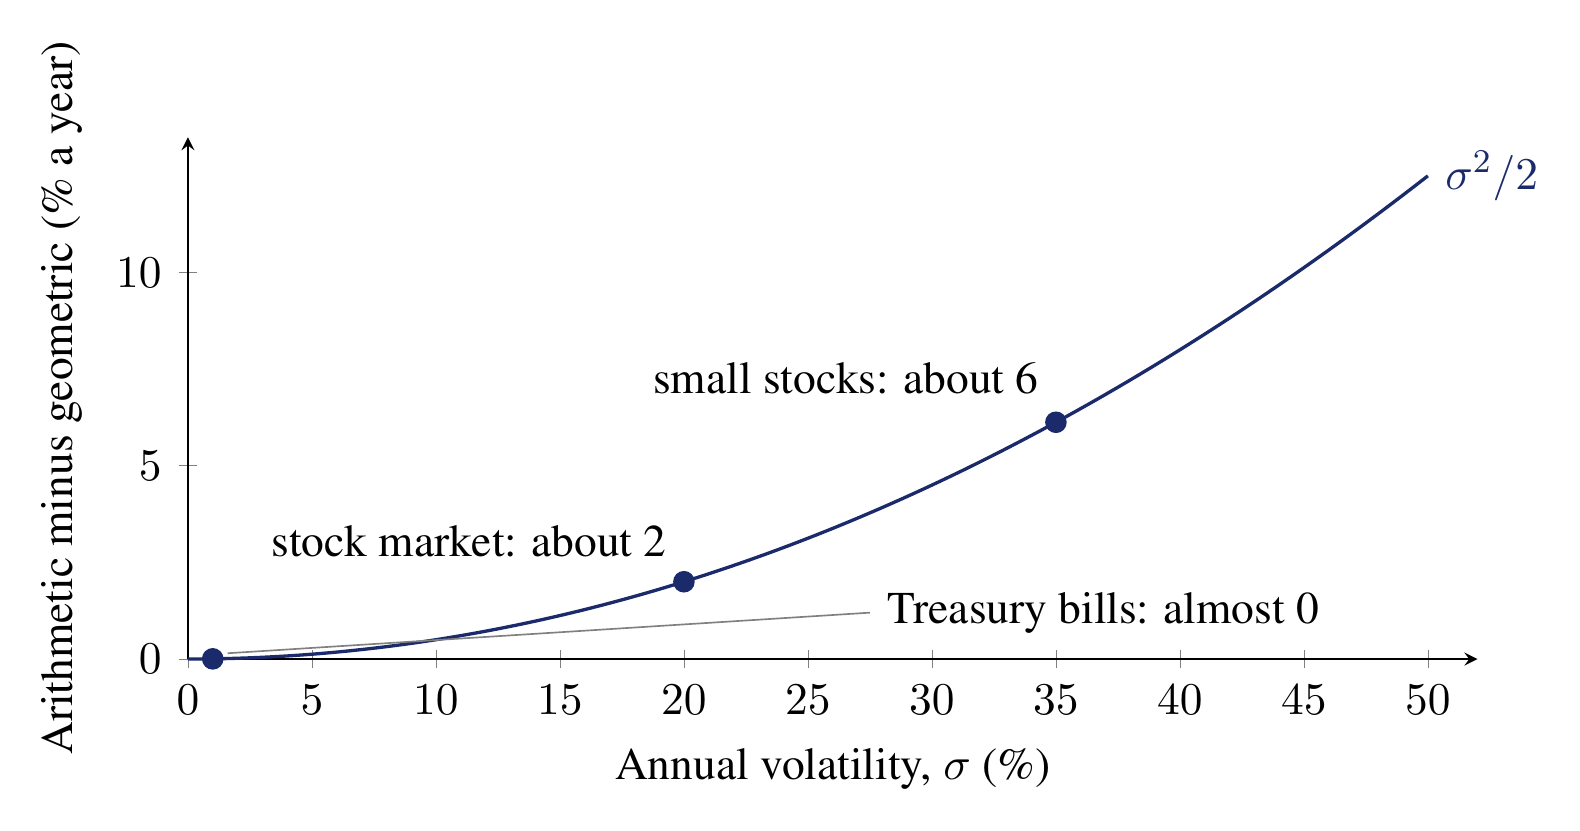
\includegraphics[width=0.85\linewidth]{images/fig02-1-volatility-drag.png}
%\caption{Volatility drag: the gap between the arithmetic and geometric average returns, from Equation~\eqref{eq:02-drag}. The gap is negligible for Treasury bills, about 2 percentage points a year for the stock market and about 6 for small stocks, and it rises with the square of volatility.}
%\label{fig:02-drag}
%\end{figure}


\providecolor{fenavy}{HTML}{1B2A6B}

\begin{figure}[!htbp]
  \centering
  \begin{tikzpicture}[
    % Arithmetic minus geometric mean = sigma^2 / 2.
    % With sigma in percent: (sigma/100)^2 / 2 * 100 = sigma^2 / 200 (% a year).
    declare function={gap(\s) = \s^2/200;}
  ]
  \begin{axis}[
    scale only axis, width=0.55\linewidth, height=0.28\linewidth,
    axis lines=left,
    axis line style={-stealth, thin},
    xmin=0, xmax=52, ymin=0, ymax=14,
    xtick={0,10,...,50},
    ytick={0,5,10},
    tick label style={font=\small},
    label style={font=\small},
    xlabel={Annual volatility, $\sigma$ (\%)},
    ylabel={Arith.\ minus geom.\ (\% a year)},
    samples=150, domain=0:50,
    clip=false,
  ]
    \addplot[fenavy, thick] {gap(x)};
    \node[fenavy, anchor=west, font=\small] at (axis cs:50.3,{gap(50)}) {$\sigma^2/2$};

    % Examples
    \fill[fenavy] (axis cs:1,{gap(1)})   circle (2pt);
    \fill[fenavy] (axis cs:20,{gap(20)}) circle (2pt);
    \fill[fenavy] (axis cs:35,{gap(35)}) circle (2pt);

    \node[anchor=south east, font=\footnotesize] at (axis cs:19.5,{gap(20)+0.2}) {stock market: about 2};
    \node[anchor=south east, font=\footnotesize] at (axis cs:34,{gap(35)+0.3}) {small stocks: about 6};
    \draw[gray!60] (axis cs:1.5,0.15) -- (axis cs:27,1.3);
    \node[anchor=west, font=\footnotesize] at (axis cs:27,1.4) {Treasury bills: almost 0};
  \end{axis}
  \end{tikzpicture}
  \caption{The more an investment swings, the more its simple average return overstates what investors actually earned. Volatility drag: the gap between the arithmetic and geometric average returns, from Equation~\eqref{eq:02-drag}. The gap is negligible for Treasury bills, about 2 percentage points a year for the stock market and about 6 for small stocks, and it rises with the square of volatility.}
  \label{fig:02-drag}
\end{figure}

\textbf{Implications:}
\begin{enumerate}
\item Use the arithmetic average when you need the expected return for a single period, as in the Sharpe ratio or a forecast, and use the geometric average when you report how much an investment grew. 
\item If you quote the arithmetic average as a growth rate, you will overstate what the investor experienced, and the overstatement is largest for the volatile strategies that tend to look most attractive. 
\item Whenever a source reports an average return, you should check which kind it is. Lab~\ref{ch:02} measures the gap on real portfolios.
\end{enumerate}

\section{Research datasets and their free alternatives}
\label{sec:02-datasets}

A result can be no more reliable than the data behind it. Each dataset covers different companies, periods and events, and each handles corrections, dividends and failed companies in its own way. 

Most published research on U.S. stocks rests on CRSP and Compustat, the two commercial databases introduced in Section~\ref{sec:02-foundations}. Two of their features\index{features and targets} matter most for this chapter, because free sources usually lack them.

\begin{itemize}
  \item \textbf{Delisting returns.}\index{return!delisting|textbf} CRSP includes companies that later disappeared, together with the return in the month in which each of them was delisted.
  \item \textbf{Point-in-time data.}\index{data!point-in-time|textbf} The point-in-time version of Compustat records what was known on each date, rather than the figures as they were later revised.
\end{itemize}

Many universities subscribe to these databases, but many readers will not have access to them. The labs in this book therefore use free sources that are either built from these databases or comparable to them:

\begingroup
\small
\setlength{\LTpre}{6pt}\setlength{\LTpost}{6pt}
\begin{longtable}{@{}>{\raggedright\arraybackslash}p{0.22\linewidth}>{\raggedright\arraybackslash}p{\dimexpr 0.9\linewidth-0.22\linewidth-0.26\linewidth-4\tabcolsep\relax}>{\raggedright\arraybackslash}p{0.26\linewidth}@{}}
\toprule
Free source & What it offers & Main limitation \\
\midrule
\endfirsthead
\multicolumn{3}{@{}l}{\emph{(continued)}} \\
\toprule
Free source & What it offers & Main limitation \\
\midrule
\endhead
\midrule
\multicolumn{3}{r@{}}{\emph{(continued on the next page)}} \\
\endfoot
\bottomrule
\endlastfoot
Kenneth R. French Data Library & Factor returns and portfolios sorted on size, value, momentum and more, built from CRSP and Compustat, since 1926 & Portfolio-level only; no individual stocks \\*
FRED (Federal Reserve Bank of St.\ Louis) & Interest rates and economic series; its ALFRED archive keeps past vintages of revised data & Economic series, not stock-level data \\
Open Source Asset Pricing (Chen and Zimmermann) & Portfolio returns for over 200 published predictors & Full firm-level signals require WRDS \\
Jensen--Kelly--Pedersen global factors & 153 factors across 93 countries & Factor-level only \\*
Yahoo Finance and similar & Daily prices for current stocks, ETFs and indexes & Mostly survivors only; adjustments not always documented; unofficial access methods can break \\
\end{longtable}
\addtocounter{table}{-1}% uncaptioned longtable: keep table numbers unchanged
\endgroup

A \textbf{predictor}, also called a \textbf{signal}, is a variable that a study uses to forecast returns, such as a \term{valuation ratio} or a past return. An ETF, or exchange-traded fund, is a fund whose shares trade on an exchange like a stock, and many ETFs simply track an index. The last row of the table deserves particular attention. Free stock-price sites are convenient, but they mostly cover companies that still exist today. A backtest that downloads today's stocks from such a site and runs them through the past therefore has survivorship bias built into it, which is the problem that Section~\ref{sec:02-survivorship} describes.

\section{Survivorship bias: the missing failures}
\label{sec:02-survivorship}

Companies that fail, merge or are delisted disappear from many datasets, and their final losses disappear with them. A backtest that is run only on companies that still exist never suffers those losses, so it overstates returns, often by several percentage points a year. This is one of the most common errors in practice, because most free price sources list only the stocks that trade today.

\subsection{Survivorship bias}

\term{Survivorship bias}\index{survivorship bias|textbf} arises when a sample includes only the companies, funds or strategies that are still around at the end of the period. Those that failed, were acquired or were shut down drop out of the data, and their losses drop out with them. It is like judging how safe a sport is by interviewing only the players who are still playing. Abraham Wald's bombers in Chapter~\ref{ch:01} teach the same lesson. A real example makes the cost concrete. Enron, once one of the largest companies in America, saw its shares fall from \$90.75 in August 2000 to 26 cents at the end of November 2001, and it filed for bankruptcy on 2 December 2001. A backtest built from the list of companies that exist today never owned Enron, so it never suffered that loss.

The bias works through three channels.

\begin{enumerate}
  \item \textbf{Survivors-only samples.} Testing a strategy on today's index members, or on the funds that exist today, removes every company or fund that failed along the way. The survivors are, by definition, the ones that did well enough to last.
  \item \textbf{Missing delisting returns.} When a stock leaves the exchange because the company is failing, its final return is often large and negative, and it is often missing from the database. Shumway (1997) checked how large this gap was in CRSP, the foundation of most research on U.S. stocks, and showed that it frequently lacked returns for delistings caused by poor performance, and he estimated that these missing returns averaged about $-30$\% for stocks on the NYSE and AMEX, the New York and American stock exchanges. Shumway and Warther (1999) found even larger losses for Nasdaq stocks, which trade on an electronic market that lists many younger and smaller companies, where failures are more common. In plain words, the data were quietly skipping the worst month in the life of many failing companies. A backtest that silently drops these months overstates returns, and the error is largest for small and distressed stocks.
  \item \textbf{Backfill.}\index{backfill bias|textbf} Databases sometimes add a company or fund only after it has already succeeded, filling in its earlier history at the same time. This \term{backfill} brings in past returns only for those that did well. Kothari, Shanken and Sloan (1995) argued that this kind of selection in Compustat inflated the measured returns of high \term{book-to-market}\index{book-to-market ratio} stocks, which are companies whose accounting value is large relative to their market value.
\end{enumerate}

The bias is well documented for mutual funds, because funds that perform badly are often closed or merged and then easily left out of a study. Elton, Gruber and Blake (1996) followed every fund, including those that vanished, and estimated that studying only the funds that survived overstated average performance by roughly 0.9 percentage points a year, which is large compared with the alphas\index{alpha} that researchers try to detect. An investor reading such a study would conclude that fund managers add value when part of that apparent value comes only from forgetting the funds that closed. Brown, Goetzmann, Ibbotson and Ross (1992) asked whether the persistence that other studies had found in fund performance might also come from the data, and showed that survivorship can even make fund performance appear to persist from one period to the next when in fact it does not.

\subsection{The problem}

\textbf{Why survivorship can create a strategy out of nothing.} Survivorship bias does not simply shift all returns upward by the same amount. Its effect is strongest for the stocks that are most likely to fail, namely small, volatile and \textbf{distressed} companies that are at real risk of bankruptcy. Among such companies, the ones that survive are the ones whose prices happened to rise. As a result, a survivors-only backtest of a strategy that buys volatile or distressed stocks can show a large premium that is produced entirely by the way the sample was built. Lab~\ref{ch:02} demonstrates this with a simulation in which the true premium is known to be zero.

\subsection{The fix}

\textbf{The fix} is to use a dataset that includes failed companies and their delisting returns, such as CRSP, together with portfolio rules that use only the firms that were listed on each date. 
Most free sources in Section~\ref{sec:02-datasets} do not need this fix. The French library, \term{Open Source Asset Pricing}\index{Open Source Asset Pricing} and the Jensen--Kelly--Pedersen data are built from CRSP, so they include companies that later failed, and \term{FRED}\index{FRED} holds economic series rather than companies. The fix matters most for free stock-price sites such as Yahoo Finance, which list mainly today's survivors. Because those sites do not show which companies are missing, the Shumway correction cannot be applied, and the safer choice is to test the strategy on portfolio data that were built from a complete database.

Researchers who work with stock-level data have a standard repair for missing delisting returns, which the shaded box describes; most readers using free data will not need it.

\begin{technote}
\textbf{Technical note: the Shumway correction.} When delisting returns are missing, researchers follow Shumway and substitute an estimate, such as $-30$\%.
Suppose a stock falls from \$10 to \$2 and is then delisted for poor performance, with no final return recorded.
If the final return is left blank, the backtest counts only the fall to \$2.
If the researcher follows Shumway, the backtest adds one more month with a $-30$\% return, as if the stock ended near \$1.40.
The estimate won’t be exact for any single company, but on average it is much closer to the truth than assuming a zero loss.
Do we need to do this fix? Probably not. Only researchers with stock-level data such as CRSP can apply it, because they can see which companies were delisted and which delisting returns are missing. Users of Yahoo Finance can’t, because the failed companies aren’t in the data at all.
\end{technote}


\section{Look-ahead bias: using only what was known}
\label{sec:02-lookahead}

A backtest is honest only if every decision in it uses information that was available at the time. Accounting figures are published weeks or months after the period they describe, and economic data are often revised later. Using the final numbers as if they had been known in advance gives a strategy an advantage that no investor had, and the result can look excellent for no real reason.

\term{Look-ahead bias}\index{look-ahead bias|textbf} arises when a backtest uses information that was not yet available when the decision would have been made. It is easy to introduce and hard to notice, because the code runs without error and the results simply look better than they should. It resembles a student who grades a practice exam with the answer key open: the score is real, but it says nothing about how the student would do on the day. Figure~\ref{fig:02-timeline} shows the most common case, in which accounting data are used before they were published.

%\begin{figure}[htbp]
%\centering
%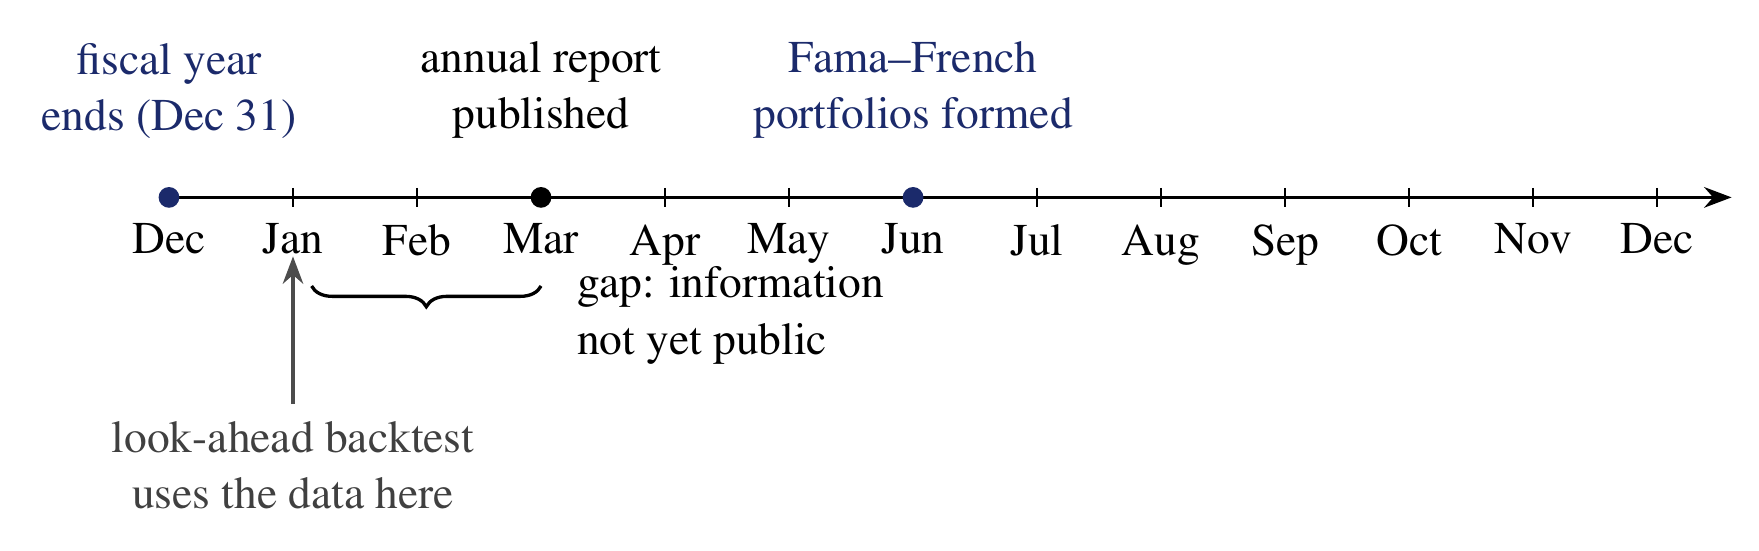
\includegraphics[width=0.9\linewidth]{images/fig02-2-accounting-timeline.png}
%\caption{When accounting data becomes usable. A company's fiscal year ends in December, but its annual report appears only months later. A backtest that trades on the figures in January uses information no investor had. Fama and French wait until the following June to be safe.}
%\label{fig:02-timeline}
%\end{figure}

\providecolor{fenavy}{HTML}{1B2A6B}
\providecolor{fegray}{HTML}{4D4D4D}

\begin{figure}[!htbp]
  \centering
  \begin{tikzpicture}[x=0.9cm, y=1cm, font=\small]
    % Timeline: Dec (0) to the following Dec (12)
    \draw[-stealth, thick] (0,0) -- (12.6,0);
    \foreach \wfI/\wfM in {0/Dec,1/Jan,2/Feb,3/Mar,4/Apr,5/May,6/Jun,
                           7/Jul,8/Aug,9/Sep,10/Oct,11/Nov,12/Dec} {
      \draw (\wfI,0.1) -- (\wfI,-0.1);
      \node[anchor=north] at (\wfI,-0.12) {\wfM};
    }

    % Key dates
    \fill[fenavy] (0,0) circle (2.6pt);
    \fill         (3,0) circle (2.6pt);
    \fill[fenavy] (6,0) circle (2.6pt);
    \node[fenavy, anchor=south, align=center] at (0,0.3)
      {fiscal year\\ends (Dec 31)};
    \node[anchor=south, align=center] at (3,0.3)
      {annual report\\published};
    \node[fenavy, anchor=south, align=center] at (6,0.3)
      {Fama--French\\portfolios formed};

    % Gap between fiscal year-end and publication
    \draw[decorate, decoration={brace, mirror, amplitude=5pt}]
      (1.1,-0.65) -- (2.9,-0.65);
    \node[anchor=north west, align=left] at (3.1,-0.5)
      {gap: information\\not yet public};

    % Look-ahead bias
    \draw[-stealth, fegray] (1,-1.9) -- (1,-0.6);
    \node[fegray, anchor=north, align=center] at (1,-2)
      {look-ahead backtest\\uses the data here};
  \end{tikzpicture}
\caption{A backtest must wait until accounting numbers were actually public before trading on them. When accounting data becomes usable. A company's fiscal year ends in December, but its annual report appears only months later. A backtest that trades on the figures in January uses information that no investor had, which is why Fama and French wait until the following June.}
\label{fig:02-timeline}
\end{figure}


The table below lists the common sources of look-ahead bias and the standard treatment against each.

\begingroup
\small
\setlength{\LTpre}{6pt}\setlength{\LTpost}{6pt}
\begin{longtable}{@{}>{\raggedleft\arraybackslash}p{0.03\linewidth}>{\raggedright\arraybackslash}p{0.16\linewidth}>{\raggedright\arraybackslash}p{\dimexpr 0.9\linewidth-0.03\linewidth-0.16\linewidth-0.32\linewidth-6\tabcolsep\relax}>{\raggedright\arraybackslash}p{0.32\linewidth}@{}}
\toprule
 & Source & What goes wrong & Standard treatment \\
\midrule
\endfirsthead
\multicolumn{4}{@{}l}{\emph{(continued)}} \\
\toprule
 & Source & What goes wrong & Standard treatment \\
\midrule
\endhead
\midrule
\multicolumn{4}{r@{}}{\emph{(continued on the next page)}} \\
\endfoot
\bottomrule
\endlastfoot
1 & Same-period execution & A signal computed from today's closing price is used to trade at that same close & Trade on the next period's return: lag every signal by at least one period \\*
2 & Accounting publication lags & Annual results for a December fiscal year are used in January, though they are published weeks or months later & Lag accounting data; Fama and French (1993) use fiscal-year data only from the following June \\
3 & Revised economic data & GDP or employment figures are used as revised years later, not as first reported & Use real-time vintages, such as FRED's ALFRED archive \\
4 & Index membership & Today's index members are used for the past & Use historical membership lists \\
5 & Full-sample choices & Parameters, thresholds or variable definitions are chosen using the whole sample, then ``tested'' on it & Choose using only data available at each date (walk-forward; Chapter~\ref{ch:06}) \\*
6 & Full-sample scaling & Signals are standardized with means and volatilities computed over the whole sample & Use expanding or rolling estimates \\
\end{longtable}
\addtocounter{table}{-1}% uncaptioned longtable: keep table numbers unchanged
\endgroup


Three terms in the table need explaining. To \textbf{lag} a signal is to use it only from a later period, so that it was already known before the trade. A \term{walk-forward}\index{walk-forward evaluation|textbf} test chooses its settings at each date using only the data available before that date, just as an investor in real time would have to. An \textbf{expanding} estimate uses all the data up to each date, whereas a \textbf{rolling} estimate uses a window of fixed length, such as the past five years. GDP, or gross domestic product, is the total value of goods and services an economy produces, and its first estimate is often revised substantially in later years. To \textbf{standardize} a signal is to rescale it so that it has an average of zero and a typical swing of one, which requires knowing its average and volatility.

The last two rows of the table describe the subtlest problems. In these cases no future price is used directly, yet the analyst's choices reflect knowledge of how the whole period turned out. For example, a trading rule whose window length was chosen because it worked best over 1926--2025 carries information from 2025 back into 1926.

\textbf{Point-in-time data}\index{data!point-in-time|textbf} is the general remedy, because it ensures that each date uses only the values that could have been known then. Lab~\ref{ch:02} measures two forms of look-ahead bias on real data, namely trading on the same day's closing price and choosing a rule's parameter with hindsight.

\section{Micro-caps: results no investor could capture}
\label{sec:02-microcaps}

The smallest companies are costly or impossible to trade in large amounts, yet in an equal-weighted portfolio they carry the same weight as the largest companies. A result can therefore be driven almost entirely by stocks that no investor could realistically buy. Checking how a portfolio is weighted, and whether its result survives without the smallest stocks, is one of the quickest ways to test whether a finding is usable.

The U.S. stock market is extremely unequal. A few hundred large companies account for most of its value, while thousands of tiny companies account for most of the names on the list. Fama and French (2008) classified stocks below the 20th percentile of NYSE market capitalization, that is, smaller than 80\% of NYSE companies, as \term{micro-caps}\index{micro-caps|textbf}, which means that each of them is smaller than four-fifths of the stocks listed on the New York Stock Exchange. They found that micro-caps made up about 60\% of all listed stocks but only about 3\% of total market value (Figure~\ref{fig:02-microcaps}).

%\begin{figure}[htbp]
%\centering
%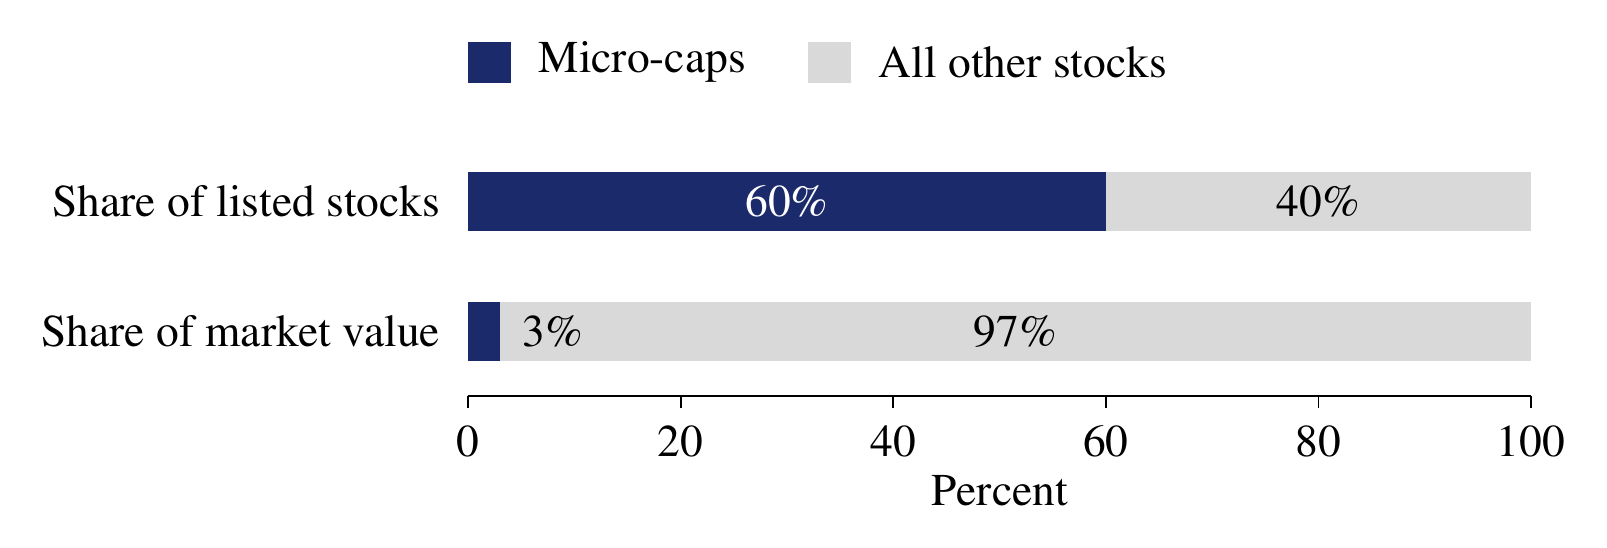
\includegraphics[width=0.8\linewidth]{images/fig02-3-microcaps.png}
%\caption{Micro-caps are most of the stocks but almost none of the money. Source: Fama and French (2008).}
%\label{fig:02-microcaps}
%\end{figure}


\providecolor{fenavy}{HTML}{1B2A6B}

\begin{figure}[!htbp]
  \centering
  \begin{tikzpicture}
  \begin{axis}[
    scale only axis, width=0.6\linewidth, height=2.4cm,
    xmin=0, xmax=100, ymin=0.4, ymax=2.6,
    axis x line*=bottom, axis y line=none,
    xtick={0,20,...,100},
    xlabel={Percent},
    xlabel style={yshift=4pt},
    clip=false,
  ]
    % Share of listed stocks: micro-caps 60%, others 40%
    \fill[fenavy]  (axis cs:0,1.7)  rectangle (axis cs:60,2.3);
    \fill[gray!25] (axis cs:60,1.7) rectangle (axis cs:100,2.3);
    \node[white] at (axis cs:30,2) {60\%};
    \node        at (axis cs:80,2) {40\%};

    % Share of market value: micro-caps 3%, others 97%
    \fill[fenavy]  (axis cs:0,0.7) rectangle (axis cs:3,1.3);
    \fill[gray!25] (axis cs:3,0.7) rectangle (axis cs:100,1.3);
    \node[anchor=west] at (axis cs:3.5,1) {3\%};
    \node              at (axis cs:51.5,1) {97\%};

    % Row labels
    \node[anchor=east] at (axis cs:-1,2) {Share of listed stocks};
    \node[anchor=east] at (axis cs:-1,1) {Share of market value};

    % Legend
    \fill[fenavy]  (axis cs:0,2.95)  rectangle (axis cs:4,3.25);
    \node[anchor=west] at (axis cs:5,3.1) {Micro-caps};
    \fill[gray!25] (axis cs:33,2.95) rectangle (axis cs:37,3.25);
    \node[anchor=west] at (axis cs:38,3.1) {All other stocks};
  \end{axis}
  \end{tikzpicture}
\caption{Micro-caps are most of the stocks but almost none of the money. Source: Fama and French (2008).}
\label{fig:02-microcaps}
\end{figure}


This matters because of the way portfolios are weighted (Section~\ref{sec:02-foundations}).

\begin{itemize}
  \item \textbf{Equal-weighted}\index{index weighting!equal-weighted|textbf} portfolios give every stock the same weight, so micro-caps dominate them simply because there are so many of them.
  \item \textbf{Value-weighted}\index{index weighting!value-weighted|textbf} portfolios weight stocks by market capitalization, so they reflect where investors' money actually is.
\end{itemize}

Micro-caps are also expensive and difficult to trade. Their \term{bid--ask spreads}\index{bid--ask spread|textbf}, the gap between the price at which you can buy and the price at which you can sell, are wide. They have little \term{liquidity}\index{liquidity|textbf}, which means that buying or selling even a modest amount moves the price. They are also costly to \term{sell short}\index{short selling|textbf}, that is, to borrow and sell in the hope of buying them back later at a lower price. In addition, micro-caps have the most extreme returns and the most data problems, including the missing delisting returns described in Section~\ref{sec:02-survivorship}. A pattern that appears in equal-weighted portfolios but not in value-weighted ones may therefore exist only where no large investor can exploit it.

The replication\index{replication} debate in Chapter~\ref{ch:15} turns partly on this point. An \term{anomaly}\index{anomaly|textbf} is a pattern in returns that standard risk models, such as the CAPM\index{capital asset pricing model (CAPM)}, cannot explain. Hou, Xue and Zhang\index{q-factor model} (2020) found that many anomalies disappear when micro-caps are given little weight, while their critics argue that this mainly shows that anomalies are concentrated among small stocks. For an investor, both readings lead to the same caution: a pattern that lives only in tiny stocks may be real, yet still impossible to profit from at any meaningful scale. Either way, the lesson for this chapter is simple: \textbf{always ask how a portfolio is weighted and whether the result survives without micro-caps.}

\begin{callout}
\textbf{What Failed: the size effect\index{size premium}.} Banz (1981) found that small companies had earned higher risk-adjusted returns than large ones, meaning higher returns even after allowing for their extra risk, and ``small beats big'' became one of the best-known findings in finance. Later research, however, found that the effect became much weaker after it was published, that it was heavily concentrated among the very smallest stocks, and that in the early studies it was concentrated in January. Size remains a common factor in models of risk, but as a stand-alone source of extra return it has been far less reliable than its early evidence suggested. Lab~\ref{ch:02} tests how much of the size premium comes from micro-caps and how much comes from the years before 1981.
\end{callout}

\section{Data snooping: when a whole field searches one dataset}
\label{sec:02-snooping}

Chapter~\ref{ch:01} described the problem of selection within one researcher's search. There is a wider version of the same problem, in which an entire field searches the same data. Most research on U.S. stocks uses CRSP, and much of it uses the same period after 1963. Thousands of researchers have tested thousands of ideas on these data, and the ideas that ``worked'' were the ones that got published. Each paper may report a single, honest test, yet together the field has run an enormous number of trials on one history. A finding can therefore be a false discovery even when its author did nothing wrong, which is why a result must be confirmed on data that played no part in finding it.

Lo and MacKinlay (1990) called this \term{data-snooping bias}\index{data snooping|textbf}. When the choice of what to test is influenced by what earlier studies found in the same data, the usual significance levels\index{hypothesis testing!significance level} overstate the strength of the evidence. No single researcher can fix this bias, because no one knows how many ideas were tried and abandoned across the whole field. A lottery offers a useful comparison. Someone wins almost every week, but the winner is not evidence that a winning system exists, because millions of tickets were bought and we hear only about the one that won.

Three defenses work, and later chapters use all of them.

\begin{enumerate}
  \item \textbf{New data.} Test the claim in periods or markets that played no part in its discovery, such as the years before the original sample, the years after publication, or other countries (Chapters~\ref{ch:04} and~\ref{ch:15}).
  \item \textbf{Higher hurdles.} Require stronger evidence for claims that are tested on heavily used data, such as a t-statistic\index{t-statistic} above 3 (Harvey, Liu and Zhu 2016; Chapter~\ref{ch:15}). The t-statistic, introduced in Chapter~\ref{ch:01}, measures how far a result stands above the noise, and the usual bar is about 2.
    \item \textbf{Economic reasoning stated in advance.} Before running a test, state why the pattern should exist. A story written after a pattern is found proves little, because a clever explanation can be invented for almost any result, including one produced by chance. A reason stated beforehand turns the test into a genuine check, because the data can prove it wrong.
\end{enumerate}

\section{Lab~\thechapter: Replicating the size effect and the survivorship and delisting biases}
\label{sec:02-lab}

\textbf{Claim on trial:} free, public data can support a reliable backtest. Each part of the lab follows one study that showed how a feature of the data can change a result. Brown, Goetzmann, Ibbotson and Ross (1992) showed by simulation that dropping funds that disappear can create false persistence, and Shumway (1997) measured the missing delisting losses. Brock, Lakonishok and LeBaron (1992) made moving-average rules famous, and Sullivan, Timmermann and White (1999) showed how much of their success came from searching across many rules. Banz (1981) discovered the size effect, and Horowitz, Loughran and Savin (2000) and Schwert (2003) found that it weakened after publication and depended on the smallest stocks. The data are monthly and daily U.S. market returns and size-sorted portfolios\index{portfolio sort} since 1926 from the Kenneth R. French Data Library\index{Kenneth French data library}, plus a simulated stock market, and the code is in the repository folder \texttt{ch02-data-traps/}. Survivorship is measured with a simulation because it requires the same backtest with and without the failed companies, and free sources do not let us take the failures out.

\textbf{Part A: Arithmetic versus geometric averages.} The lab computes both averages for Treasury bills, the market, and the largest and smallest 10\% of stocks, and compares each gap with the volatility-drag approximation $G \approx A - \sigma^2/2$\index{variance} of Section~\ref{sec:02-returns} (Lab Figure~\ref{ch:02}.1). Expect almost no gap for Treasury bills, about 2 percentage points a year for the market, and several points for the smallest stocks.

\textbf{Part B: Survivorship bias in a market where the truth is known.} Following Brown and colleagues (1992), the lab simulates about 2,000 listed companies over 30 years, all with the \textbf{same expected return}, so no stock or strategy has a real advantage. Following Shumway (1997), a company whose price falls below 20\% of its listing price is delisted with a final return of $-30$\%. From this one history the lab builds three datasets: the full data, the same data without the final delisting month, and the survivors only. On each, it measures the equal-weighted market return and a strategy that buys the most volatile fifth of stocks and sells the least volatile fifth (Lab Figure~\ref{ch:02}.2). With the default settings (seed 2026):

\begingroup
\small
\setlength{\LTpre}{6pt}\setlength{\LTpost}{6pt}
\begin{longtable}{@{}>{\raggedright\arraybackslash}p{\dimexpr 0.9\linewidth-0.22\linewidth-0.22\linewidth-0.12\linewidth-6\tabcolsep\relax}>{\raggedright\arraybackslash}p{0.22\linewidth}>{\raggedright\arraybackslash}p{0.22\linewidth}>{\raggedleft\arraybackslash}p{0.12\linewidth}@{}}
\toprule
Dataset & Equal-weighted compound return & Volatile minus calm, per year & t-statistic \\
\midrule
\endfirsthead
\multicolumn{4}{@{}l}{\emph{(continued)}} \\
\toprule
Dataset & Equal-weighted compound return & Volatile minus calm, per year & t-statistic \\
\midrule
\endhead
\midrule
\multicolumn{4}{r@{}}{\emph{(continued on the next page)}} \\
\endfoot
\bottomrule
\endlastfoot
Full data & 9.3\% & $-1.2$\% & $-2.2$ \\*
Missing delisting returns & 10.7\% & $+2.0$\% & 3.5 \\*
Survivors only & 14.0\% & $+12.0$\% & 14.7 \\*
\end{longtable}
\addtocounter{table}{-1}% uncaptioned longtable: keep table numbers unchanged
\endgroup

Leaving out only the delisting returns flips the strategy's loss into a gain, and keeping only the survivors adds almost five points a year to the market's return and creates a ``volatility premium'' of 12\% a year with a t-statistic of 14.7. None of it is real.

\textbf{Part C: Look-ahead bias.} A rule holds stocks when the market closes above its 200-day \textbf{moving average}\index{moving average|textbf} and Treasury bills otherwise. The correct version decides at yesterday's close; the look-ahead version decides at today's close but is still credited with today's return (Lab Figure~\ref{ch:02}.3). The lab then tests windows from 20 to 300 days and compares the window chosen with hindsight over the whole period with one chosen each January from the results so far (Lab Figure~\ref{ch:02}.4). The gap measures the inflation from choosing settings after seeing the results.

\textbf{Part D: Micro-caps, weighting and the size premium.} The lab measures the \term{size premium}\index{size premium|textbf}, the smallest tenth of stocks minus the largest tenth, with value and equal weights, each with and without the smallest tenth, before and after Banz's 1981 publication (Lab Figure~\ref{ch:02}.5). If the premium lives mainly in tiny stocks or disappeared after publication, the claim weakens.

% [Draft note: figures and numbers for Parts A, C and D are generated from the Kenneth R. French data at the time of publication; the book prints those results. The Part B simulation is fixed by design and its results can be printed as they stand.]

The lab ends by asking you to write one sentence for each problem, reach your own verdict on the scale of Section~\ref{sec:01-method}, and compare it with Section~\ref{sec:02-verdict}.

\section{Where the evidence stands}
\label{sec:02-verdict}

The published studies point to a clear pattern: \textbf{free, public data can support a reliable backtest, but only when the data include failed companies and the backtest avoids hindsight and checks how its portfolios are weighted.} The table summarizes the evidence as of November 2026.

\begingroup
\small
\setlength{\LTpre}{6pt}\setlength{\LTpost}{6pt}
\begin{longtable}{@{}>{\raggedright\arraybackslash}p{0.19\linewidth}>{\raggedright\arraybackslash}p{0.13\linewidth}>{\raggedright\arraybackslash}p{\dimexpr \linewidth-0.19\linewidth-0.13\linewidth-0.23\linewidth-6\tabcolsep\relax}>{\raggedright\arraybackslash}p{0.23\linewidth}@{}}
\toprule
Situation & Holds? & Why & Evidence \\
\midrule
\endfirsthead
\multicolumn{4}{@{}l}{\emph{(continued)}} \\
\toprule
Situation & Holds? & Why & Evidence \\
\midrule
\endhead
\midrule
\multicolumn{4}{r@{}}{\emph{(continued on the next page)}} \\
\endfoot
\bottomrule
\endlastfoot
Portfolio data from the French library and similar sources & \textbf{Yes} & These data are built from CRSP, so they include companies that later failed, together with their delisting returns. & Kenneth R. French Data Library; Chen and Zimmermann; Jensen, Kelly and Pedersen \\*
\addlinespace[3pt]
Today's stocks from a free price site & \textbf{No} & The companies that failed are missing, so returns are overstated and false patterns can appear. & Brown, Goetzmann, Ibbotson and Ross (1992); Elton, Gruber and Blake (1996) \\
\addlinespace[3pt]
Data with missing delisting returns & \textbf{No} & The final losses of failing companies, about $-30$\% on average and more on Nasdaq, are left out. & Shumway (1997); Shumway and Warther (1999) \\
\addlinespace[3pt]
Signals or settings chosen with hindsight & \textbf{No} & Using figures before they were published, or choosing a rule's settings over the whole sample, makes results look better than any investor could have achieved. & Fama and French (1993); Sullivan, Timmermann and White (1999) \\
\addlinespace[3pt]
Equal-weighted results & \textbf{Partly} & Micro-caps are about 60\% of listed stocks but only 3\% of market value, and many anomalies disappear without them. & Fama and French (2008); Hou, Xue and Zhang (2020) \\*
\addlinespace[3pt]
Findings tested only on the data where they were found & \textbf{Partly} & The whole field has searched the same data, and effects such as size weakened after they were published. & Lo and MacKinlay (1990); Schwert (2003); Harvey, Liu and Zhu (2016) \\
\end{longtable}
\addtocounter{table}{-1}% uncaptioned longtable: keep table numbers unchanged
\endgroup

A backtest built on free data can therefore be trusted only if it uses the right returns, includes the failures, uses only what was known at the time and checks its weighting. The checklist in Section~\ref{sec:02-checklist} turns these conditions into questions.

\textbf{What would change the picture.} The claim would gain broader support if free sources published stock-level data that include delisted companies, and would weaken if the CRSP-based portfolio data were found to contain errors that change published results.

\section{What practitioners and investors can use: a data checklist}
\label{sec:02-checklist}

Before you trust any backtest, your own or someone else's, work through these questions. Most take a few minutes.

\begin{itemize}
  \item[$\square$] \textbf{Returns (Section~\ref{sec:02-returns}):} Are they total returns above the risk-free rate, compared with a total-return benchmark? Is the average arithmetic or geometric?
  \item[$\square$] \textbf{Survivorship (Section~\ref{sec:02-survivorship}):} Are companies or funds that no longer exist included, with their delisting returns?
  \item[$\square$] \textbf{Look-ahead (Section~\ref{sec:02-lookahead}):} Is every signal lagged, and were any parameters, thresholds or universes chosen using the whole sample?
  \item[$\square$] \textbf{Weighting (Section~\ref{sec:02-microcaps}):} Is the portfolio value- or equal-weighted, and does the result survive without micro-caps?
  \item[$\square$] \textbf{Shared data (Section~\ref{sec:02-snooping}):} Has the result been tested on other periods, other markets or the years after publication?
\end{itemize}

% Key terms that this chapter uses without defining them, for readers new to finance.
\providecolor{FEMaroon}{RGB}{128,30,45}
\providecolor{FECream}{RGB}{253,248,238}
\providecolor{FEGold}{RGB}{196,150,60}
\makeatletter
\@ifundefined{keyterms}{%
  \newtcolorbox{keyterms}[1][Key terms in this chapter]{breakable, enhanced,
    colback=FECream, colframe=FEGold, boxrule=0.6pt, arc=2pt, leftrule=3pt,
    left=8pt, right=8pt, top=6pt, bottom=6pt, before skip=12pt, after skip=12pt,
    fonttitle=\bfseries, coltitle=white, colbacktitle=FEMaroon, title={#1}}%
}{}
\makeatother

\begin{keyterms}
\small
\begin{description}[leftmargin=0pt, itemsep=2pt, parsep=0pt, font=\normalfont\bfseries\color{FEMaroon}]
  \item[Compustat.] Compustat is the standard subscription database of companies' accounting data, such as earnings and book values.
  \item[CRSP.] CRSP, the Center for Research in Security Prices, is the standard subscription database of U.S. stock prices and returns, including companies that no longer exist.
  \item[FRED.] FRED is the Federal Reserve Bank of St.~Louis's free online database of economic and financial series, such as interest rates and inflation.
  \item[Open Source Asset Pricing.] See Chapter~\ref{ch:15}, Section~\ref{sec:19-how}, page~\pageref{sec:19-how}.
  \item[Rebalancing.] Rebalancing means buying and selling to bring a portfolio's weights back to their targets after prices have moved.
\end{description}
\end{keyterms}
   % historical data show what a strategy would have earned

% ---- Part II: The Classical Cross-Section
\part{The Classical Cross-Section}
% Chapter 4 -- Claim: Size and Value Explain Returns That Beta Cannot
% Figures need tikz and pgfplots (with the fillbetween library) in the preamble.
\providecolor{fenavy}{HTML}{1B2A6B}
\providecolor{fegray}{HTML}{4D4D4D}
\providecolor{feshade}{HTML}{F3F5FA}
% Shaded box for optional technical material that general readers may skip.
\makeatletter
\@ifundefined{technote}{%
  \newtcolorbox{technote}{breakable, enhanced,
    colback=feshade, colframe=fenavy!60, boxrule=0.5pt, arc=1mm,
    left=8pt, right=8pt, top=4pt, bottom=4pt}%
}{}
\makeatother

\chapter{Claim: Size and Value Explain Returns That Beta Cannot}
\label{ch:03}

Financial websites list a number called ``beta'' next to every stock, and fund brochures describe their funds with labels such as ``small-cap value'' or ``large-cap growth.'' These everyday labels come straight from the research in this chapter. They rest on a simple question that every investor eventually asks: why do some stocks earn more than others over the long run, and is a fund that beats the market showing skill, or just holding a particular kind of stock?

In the 1960s, finance seemed to have a complete answer to one of its oldest questions: why do some stocks earn more than others on average? The Capital Asset Pricing Model of Sharpe (1964) said that a stock's expected return depends on a single number, its \textbf{beta} with the market, as described in Equation~\ref{eq:ch01_beta} and later in Equation~\ref{eq:04-capm}. The answer was elegant, because it said exactly what should \emph{not} matter. For example, a company's size, its price relative to its earnings or book value, and its own volatility should tell an investor nothing about its future return once beta is known.

The model was soon challenged. The early tests of Black, Jensen and Scholes (1972) and Fama and MacBeth (1973) checked the model's sharpest prediction, that average returns rise with beta along a straight line, and found that returns did rise with beta, though less steeply than the theory said. Over the next decade, researchers tested the other half of the prediction, that nothing besides beta should matter, and more patterns were discovered.
Basu (1977) asked whether stocks that look cheap relative to their profits could beat an efficient market, and found that stocks with low price--earnings ratios earned more than their betas predicted. Banz (1981) found the same for small companies, and Rosenberg, Reid and Lanstein (1985), looking for evidence of mispricing, found it for stocks with high book-to-market ratios. A price--earnings ratio compares a share's price with the company's profit per share, and a book-to-market ratio compares the company's accounting value with its value on the stock market. Stocks that look cheap on these measures are called \emph{value} stocks, and those that look expensive are called \emph{growth} stocks.

Even so, the CAPM remains the standard way to think about the trade-off between risk and return, because it separates the risk that diversification removes from the risk that investors must be paid to bear. In practice it is still the most common tool for estimating the cost of equity, which is the return a company's shareholders expect and therefore the return its new projects must beat: Graham and Harvey (2001) found that about three quarters of the chief financial officers they surveyed used it, and it remains a staple of valuation, capital budgeting and the regulation of utility rates. 

These findings mattered because of what they might mean. 
Fama (1970) had pointed out that market efficiency can only be tested together with a model of expected returns. An anomaly therefore always has two explanations: either the market is inefficient and misprices stocks, or the market is efficient and the model of risk is wrong.
The question came to a head when Fama and French (1992) showed that, once size and book-to-market were taken into account, beta had almost no power to explain average returns. The finding made headlines, and newspapers summed it up as ``beta is dead.'' Fama and French (1993) then proposed that size and value capture risks the market factor misses, and built the three-factor model on that idea. 

Lakonishok, Shleifer and Vishny (1994) offered the opposite reading, and with it a challenge to the efficient market hypothesis. In their view, value stocks earn more not because they are riskier, but because investors make predictable mistakes. Investors extrapolate past growth too far and overreact to bad news, so they pay too much for glamour stocks with strong recent growth and too little for value stocks with weak recent growth. Overreaction of this kind is a form of mispricing, and the higher returns of value stocks are what investors earn as prices correct. Lakonishok, Shleifer and Vishny also found that value stocks did not do worse than growth stocks in recessions or market declines, which is hard to square with a story about risk. The same numbers therefore supported two stories: in one the market is efficient and the extra return is payment for risk, and in the other the market is inefficient and the extra return comes from investors' mistakes.

The answer has large practical consequences. It decides what counts as skill when a fund manager beats the market, since a manager who simply holds small value stocks may earn a high CAPM alpha and no alpha at all against three factors. It affects the discount rate companies use for new projects (Graham and Harvey 2001), and it underpins the factor and smart-beta funds that now manage large sums for ordinary investors. A smart-beta fund is an index-like fund that deliberately tilts toward stocks with certain characteristics, such as small size or low prices relative to earnings. As researchers have since proposed several hundred factors, the question has also become a statistical one: how many of these factors are real, and how many are the product of searching through the same data? 

The claim on trial\index{claims-on-trial method} in this chapter is therefore: \textbf{additional factors such as size and value explain differences in portfolio returns that beta cannot, but testing many candidate factors produces false discoveries, so a new factor must clear a higher bar.}

The chapter is built around Fama and French (1993, 2015), who showed that size, value, profitability and investment factors explain differences in returns that beta alone cannot. It also draws on Harvey, Liu and Zhu (2016), who warn that testing hundreds of candidate factors produces false discoveries. The lab in Section~\ref{sec:04-lab} replicates the Fama--French (1993) time-series regressions on their 25 size and book-to-market portfolios, in order to check whether the added factors really explain returns better than the CAPM, and then runs a factor-zoo experiment in order to see how many factors chance alone would appear to discover.

By the end of the chapter you will be able to:
\begin{itemize}
  \item summarize a return distribution by its mean, variance, skewness, kurtosis and autocorrelation, and run and interpret a linear regression;
  \item trace the path from the CAPM to the Fama--French three- and five-factor models and the factor zoo, and interpret beta, alpha and factor loadings at each step;
  \item split a portfolio's total variance into systematic and idiosyncratic parts;
  \item test whether factors are priced with the GRS test and Fama--MacBeth regressions;
  \item explain why searching through many factors produces false discoveries, and apply a stricter hurdle such as $t > 3$;
  \item separate statistical from economic significance, and judge what multi-factor models mean for asset management, performance attribution and corporate finance.
\end{itemize}

In the lab you will replicate the main regressions of Fama and French (1993), decompose the risk of their 25 classic portfolios, measure the stylized facts of returns on real data, compute the portfolios' alphas under four standard error methods, and run a controlled experiment showing how overlapping long-horizon regressions find predictability that is not there.


\section{Foundations: Distributions and Regression}
\label{sec:04-foundations}

This section collects the basic tools that the rest of the chapter builds on.
Readers who know this material can skim it then go to Section \ref{sec:04-decomposition}, but the notation introduced here is used throughout the book.

\subsection{Describing a Distribution}
Four numbers, called \textbf{moments}, summarize a return distribution:
\begin{itemize}
  \item The \textbf{mean}\index{mean} is its center: the average return.
  \item The \textbf{variance}\index{variance|textbf}, or its square root the standard deviation\index{standard deviation}, measures spread: how far returns typically fall from the mean.
  \item \textbf{Skewness}\index{skewness|textbf} measures asymmetry. It is negative when large losses are more likely than large gains of the same size, as for most stock indexes. On 19 October 1987, for example, the Dow Jones Industrial Average fell 22.6\% in a single day, a loss far larger than any single-day gain in its history.
  \item \textbf{Kurtosis}\index{kurtosis|textbf} measures tail heaviness. A normal distribution has kurtosis 3; values above 3 indicate \textbf{fat tails}\index{fat tails|textbf}, meaning extreme returns occur far more often than a normal distribution predicts.
\end{itemize}

Figure~\ref{fig:04-moments} shows what each moment changes, by comparing the normal distribution with one that differs in that moment alone. The first two moments are the ones most investors already use: an average return and a volatility. The last two are the ones most often ignored, and they are the ones that matter most when markets turn violent. Two portfolios can have the same mean and the same standard deviation, yet one can lose 20\% in a day far more often than the other.

%\begin{figure}[htbp]
%\centering
%\includegraphics[width=0.7\linewidth]{images/fig03-0-moments.pdf}
%\caption{The four moments of a distribution. Each panel compares the standard normal distribution (solid) with one that differs in a single respect. (a)~The mean sets the center. (b)~The variance sets the spread. (c)~Negative skewness lengthens the left tail, so large losses are more likely than large gains of the same size. (d)~Higher kurtosis puts more weight in the tails: the normal distribution has kurtosis 3, the fat-tailed one shown has kurtosis 9. Panels (c) and (d) keep the mean and variance of the normal distribution.}
%\label{fig:04-moments}
%\end{figure}

\begin{figure}[htbp]
\centering
\begin{tikzpicture}[font=\small]
\pgfplotsset{
  panel/.style={width=6.6cm, height=5cm, axis lines=left, xmin=-6, xmax=6, ymin=0,
    xtick={-4,-2,0,2,4}, ytick=\empty, clip=false,
    title style={font=\footnotesize}, every tick label/.style={font=\small}},
  normal/.style={fenavy, thick, no marks},
  comp/.style={fegray, thick, dashed, no marks},
}
% (a) mean
\begin{axis}[panel, name=a, ymax=0.5, ylabel={Likelihood},
  title={(a) Mean: where the distribution is centered}]
\addplot[normal] coordinates {(-6.000,0.00000) (-5.950,0.00000) (-5.900,0.00000) (-5.850,0.00000) (-5.800,0.00000) (-5.750,0.00000) (-5.700,0.00000) (-5.650,0.00000) (-5.600,0.00000) (-5.550,0.00000) (-5.500,0.00000) (-5.450,0.00000) (-5.400,0.00000) (-5.350,0.00000) (-5.300,0.00000) (-5.250,0.00000) (-5.200,0.00000) (-5.150,0.00000) (-5.100,0.00000) (-5.050,0.00000) (-5.000,0.00000) (-4.950,0.00000) (-4.900,0.00000) (-4.850,0.00000) (-4.800,0.00000) (-4.750,0.00001) (-4.700,0.00001) (-4.650,0.00001) (-4.600,0.00001) (-4.550,0.00001) (-4.500,0.00002) (-4.450,0.00002) (-4.400,0.00002) (-4.350,0.00003) (-4.300,0.00004) (-4.250,0.00005) (-4.200,0.00006) (-4.150,0.00007) (-4.100,0.00009) (-4.050,0.00011) (-4.000,0.00013) (-3.950,0.00016) (-3.900,0.00020) (-3.850,0.00024) (-3.800,0.00029) (-3.750,0.00035) (-3.700,0.00042) (-3.650,0.00051) (-3.600,0.00061) (-3.550,0.00073) (-3.500,0.00087) (-3.450,0.00104) (-3.400,0.00123) (-3.350,0.00146) (-3.300,0.00172) (-3.250,0.00203) (-3.200,0.00238) (-3.150,0.00279) (-3.100,0.00327) (-3.050,0.00381) (-3.000,0.00443) (-2.950,0.00514) (-2.900,0.00595) (-2.850,0.00687) (-2.800,0.00792) (-2.750,0.00909) (-2.700,0.01042) (-2.650,0.01191) (-2.600,0.01358) (-2.550,0.01545) (-2.500,0.01753) (-2.450,0.01984) (-2.400,0.02239) (-2.350,0.02522) (-2.300,0.02833) (-2.250,0.03174) (-2.200,0.03547) (-2.150,0.03955) (-2.100,0.04398) (-2.050,0.04879) (-2.000,0.05399) (-1.950,0.05959) (-1.900,0.06562) (-1.850,0.07206) (-1.800,0.07895) (-1.750,0.08628) (-1.700,0.09405) (-1.650,0.10226) (-1.600,0.11092) (-1.550,0.12001) (-1.500,0.12952) (-1.450,0.13943) (-1.400,0.14973) (-1.350,0.16038) (-1.300,0.17137) (-1.250,0.18265) (-1.200,0.19419) (-1.150,0.20594) (-1.100,0.21785) (-1.050,0.22988) (-1.000,0.24197) (-0.950,0.25406) (-0.900,0.26609) (-0.850,0.27798) (-0.800,0.28969) (-0.750,0.30114) (-0.700,0.31225) (-0.650,0.32297) (-0.600,0.33322) (-0.550,0.34294) (-0.500,0.35207) (-0.450,0.36053) (-0.400,0.36827) (-0.350,0.37524) (-0.300,0.38139) (-0.250,0.38667) (-0.200,0.39104) (-0.150,0.39448) (-0.100,0.39695) (-0.050,0.39844) (0.000,0.39894) (0.050,0.39844) (0.100,0.39695) (0.150,0.39448) (0.200,0.39104) (0.250,0.38667) (0.300,0.38139) (0.350,0.37524) (0.400,0.36827) (0.450,0.36053) (0.500,0.35207) (0.550,0.34294) (0.600,0.33322) (0.650,0.32297) (0.700,0.31225) (0.750,0.30114) (0.800,0.28969) (0.850,0.27798) (0.900,0.26609) (0.950,0.25406) (1.000,0.24197) (1.050,0.22988) (1.100,0.21785) (1.150,0.20594) (1.200,0.19419) (1.250,0.18265) (1.300,0.17137) (1.350,0.16038) (1.400,0.14973) (1.450,0.13943) (1.500,0.12952) (1.550,0.12001) (1.600,0.11092) (1.650,0.10226) (1.700,0.09405) (1.750,0.08628) (1.800,0.07895) (1.850,0.07206) (1.900,0.06562) (1.950,0.05959) (2.000,0.05399) (2.050,0.04879) (2.100,0.04398) (2.150,0.03955) (2.200,0.03547) (2.250,0.03174) (2.300,0.02833) (2.350,0.02522) (2.400,0.02239) (2.450,0.01984) (2.500,0.01753) (2.550,0.01545) (2.600,0.01358) (2.650,0.01191) (2.700,0.01042) (2.750,0.00909) (2.800,0.00792) (2.850,0.00687) (2.900,0.00595) (2.950,0.00514) (3.000,0.00443) (3.050,0.00381) (3.100,0.00327) (3.150,0.00279) (3.200,0.00238) (3.250,0.00203) (3.300,0.00172) (3.350,0.00146) (3.400,0.00123) (3.450,0.00104) (3.500,0.00087) (3.550,0.00073) (3.600,0.00061) (3.650,0.00051) (3.700,0.00042) (3.750,0.00035) (3.800,0.00029) (3.850,0.00024) (3.900,0.00020) (3.950,0.00016) (4.000,0.00013) (4.050,0.00011) (4.100,0.00009) (4.150,0.00007) (4.200,0.00006) (4.250,0.00005) (4.300,0.00004) (4.350,0.00003) (4.400,0.00002) (4.450,0.00002) (4.500,0.00002) (4.550,0.00001) (4.600,0.00001) (4.650,0.00001) (4.700,0.00001) (4.750,0.00001) (4.800,0.00000) (4.850,0.00000) (4.900,0.00000) (4.950,0.00000) (5.000,0.00000) (5.050,0.00000) (5.100,0.00000) (5.150,0.00000) (5.200,0.00000) (5.250,0.00000) (5.300,0.00000) (5.350,0.00000) (5.400,0.00000) (5.450,0.00000) (5.500,0.00000) (5.550,0.00000) (5.600,0.00000) (5.650,0.00000) (5.700,0.00000) (5.750,0.00000) (5.800,0.00000) (5.850,0.00000) (5.900,0.00000) (5.950,0.00000) (6.000,0.00000)};
\addplot[comp] coordinates {(-6.000,0.00000) (-5.950,0.00000) (-5.900,0.00000) (-5.850,0.00000) (-5.800,0.00000) (-5.750,0.00000) (-5.700,0.00000) (-5.650,0.00000) (-5.600,0.00000) (-5.550,0.00000) (-5.500,0.00000) (-5.450,0.00000) (-5.400,0.00000) (-5.350,0.00000) (-5.300,0.00000) (-5.250,0.00000) (-5.200,0.00000) (-5.150,0.00000) (-5.100,0.00000) (-5.050,0.00000) (-5.000,0.00000) (-4.950,0.00000) (-4.900,0.00000) (-4.850,0.00000) (-4.800,0.00000) (-4.750,0.00000) (-4.700,0.00000) (-4.650,0.00000) (-4.600,0.00000) (-4.550,0.00000) (-4.500,0.00000) (-4.450,0.00000) (-4.400,0.00000) (-4.350,0.00000) (-4.300,0.00000) (-4.250,0.00000) (-4.200,0.00000) (-4.150,0.00000) (-4.100,0.00000) (-4.050,0.00000) (-4.000,0.00000) (-3.950,0.00000) (-3.900,0.00000) (-3.850,0.00000) (-3.800,0.00000) (-3.750,0.00000) (-3.700,0.00000) (-3.650,0.00000) (-3.600,0.00000) (-3.550,0.00000) (-3.500,0.00000) (-3.450,0.00000) (-3.400,0.00000) (-3.350,0.00000) (-3.300,0.00000) (-3.250,0.00000) (-3.200,0.00000) (-3.150,0.00000) (-3.100,0.00000) (-3.050,0.00000) (-3.000,0.00000) (-2.950,0.00000) (-2.900,0.00000) (-2.850,0.00000) (-2.800,0.00000) (-2.750,0.00001) (-2.700,0.00001) (-2.650,0.00001) (-2.600,0.00001) (-2.550,0.00001) (-2.500,0.00002) (-2.450,0.00002) (-2.400,0.00002) (-2.350,0.00003) (-2.300,0.00004) (-2.250,0.00005) (-2.200,0.00006) (-2.150,0.00007) (-2.100,0.00009) (-2.050,0.00011) (-2.000,0.00013) (-1.950,0.00016) (-1.900,0.00020) (-1.850,0.00024) (-1.800,0.00029) (-1.750,0.00035) (-1.700,0.00042) (-1.650,0.00051) (-1.600,0.00061) (-1.550,0.00073) (-1.500,0.00087) (-1.450,0.00104) (-1.400,0.00123) (-1.350,0.00146) (-1.300,0.00172) (-1.250,0.00203) (-1.200,0.00238) (-1.150,0.00279) (-1.100,0.00327) (-1.050,0.00381) (-1.000,0.00443) (-0.950,0.00514) (-0.900,0.00595) (-0.850,0.00687) (-0.800,0.00792) (-0.750,0.00909) (-0.700,0.01042) (-0.650,0.01191) (-0.600,0.01358) (-0.550,0.01545) (-0.500,0.01753) (-0.450,0.01984) (-0.400,0.02239) (-0.350,0.02522) (-0.300,0.02833) (-0.250,0.03174) (-0.200,0.03547) (-0.150,0.03955) (-0.100,0.04398) (-0.050,0.04879) (0.000,0.05399) (0.050,0.05959) (0.100,0.06562) (0.150,0.07206) (0.200,0.07895) (0.250,0.08628) (0.300,0.09405) (0.350,0.10226) (0.400,0.11092) (0.450,0.12001) (0.500,0.12952) (0.550,0.13943) (0.600,0.14973) (0.650,0.16038) (0.700,0.17137) (0.750,0.18265) (0.800,0.19419) (0.850,0.20594) (0.900,0.21785) (0.950,0.22988) (1.000,0.24197) (1.050,0.25406) (1.100,0.26609) (1.150,0.27798) (1.200,0.28969) (1.250,0.30114) (1.300,0.31225) (1.350,0.32297) (1.400,0.33322) (1.450,0.34294) (1.500,0.35207) (1.550,0.36053) (1.600,0.36827) (1.650,0.37524) (1.700,0.38139) (1.750,0.38667) (1.800,0.39104) (1.850,0.39448) (1.900,0.39695) (1.950,0.39844) (2.000,0.39894) (2.050,0.39844) (2.100,0.39695) (2.150,0.39448) (2.200,0.39104) (2.250,0.38667) (2.300,0.38139) (2.350,0.37524) (2.400,0.36827) (2.450,0.36053) (2.500,0.35207) (2.550,0.34294) (2.600,0.33322) (2.650,0.32297) (2.700,0.31225) (2.750,0.30114) (2.800,0.28969) (2.850,0.27798) (2.900,0.26609) (2.950,0.25406) (3.000,0.24197) (3.050,0.22988) (3.100,0.21785) (3.150,0.20594) (3.200,0.19419) (3.250,0.18265) (3.300,0.17137) (3.350,0.16038) (3.400,0.14973) (3.450,0.13943) (3.500,0.12952) (3.550,0.12001) (3.600,0.11092) (3.650,0.10226) (3.700,0.09405) (3.750,0.08628) (3.800,0.07895) (3.850,0.07206) (3.900,0.06562) (3.950,0.05959) (4.000,0.05399) (4.050,0.04879) (4.100,0.04398) (4.150,0.03955) (4.200,0.03547) (4.250,0.03174) (4.300,0.02833) (4.350,0.02522) (4.400,0.02239) (4.450,0.01984) (4.500,0.01753) (4.550,0.01545) (4.600,0.01358) (4.650,0.01191) (4.700,0.01042) (4.750,0.00909) (4.800,0.00792) (4.850,0.00687) (4.900,0.00595) (4.950,0.00514) (5.000,0.00443) (5.050,0.00381) (5.100,0.00327) (5.150,0.00279) (5.200,0.00238) (5.250,0.00203) (5.300,0.00172) (5.350,0.00146) (5.400,0.00123) (5.450,0.00104) (5.500,0.00087) (5.550,0.00073) (5.600,0.00061) (5.650,0.00051) (5.700,0.00042) (5.750,0.00035) (5.800,0.00029) (5.850,0.00024) (5.900,0.00020) (5.950,0.00016) (6.000,0.00013)};
\draw[fenavy, densely dotted] (axis cs:0,0) -- (axis cs:0,0.45);
\draw[fegray, densely dotted] (axis cs:2,0) -- (axis cs:2,0.45);
\node[fenavy, anchor=south east] at (axis cs:-0.05,0.42) {mean 0};
\node[fegray, anchor=south west] at (axis cs:2.05,0.42) {mean 2};
\end{axis}
% (b) variance
\begin{axis}[panel, name=b, at={($(a.east)+(1.2cm,0)$)}, anchor=west, ymax=0.5,
  title={(b) Variance: how widely returns spread}]
\addplot[normal] coordinates {(-6.000,0.00000) (-5.950,0.00000) (-5.900,0.00000) (-5.850,0.00000) (-5.800,0.00000) (-5.750,0.00000) (-5.700,0.00000) (-5.650,0.00000) (-5.600,0.00000) (-5.550,0.00000) (-5.500,0.00000) (-5.450,0.00000) (-5.400,0.00000) (-5.350,0.00000) (-5.300,0.00000) (-5.250,0.00000) (-5.200,0.00000) (-5.150,0.00000) (-5.100,0.00000) (-5.050,0.00000) (-5.000,0.00000) (-4.950,0.00000) (-4.900,0.00000) (-4.850,0.00000) (-4.800,0.00000) (-4.750,0.00001) (-4.700,0.00001) (-4.650,0.00001) (-4.600,0.00001) (-4.550,0.00001) (-4.500,0.00002) (-4.450,0.00002) (-4.400,0.00002) (-4.350,0.00003) (-4.300,0.00004) (-4.250,0.00005) (-4.200,0.00006) (-4.150,0.00007) (-4.100,0.00009) (-4.050,0.00011) (-4.000,0.00013) (-3.950,0.00016) (-3.900,0.00020) (-3.850,0.00024) (-3.800,0.00029) (-3.750,0.00035) (-3.700,0.00042) (-3.650,0.00051) (-3.600,0.00061) (-3.550,0.00073) (-3.500,0.00087) (-3.450,0.00104) (-3.400,0.00123) (-3.350,0.00146) (-3.300,0.00172) (-3.250,0.00203) (-3.200,0.00238) (-3.150,0.00279) (-3.100,0.00327) (-3.050,0.00381) (-3.000,0.00443) (-2.950,0.00514) (-2.900,0.00595) (-2.850,0.00687) (-2.800,0.00792) (-2.750,0.00909) (-2.700,0.01042) (-2.650,0.01191) (-2.600,0.01358) (-2.550,0.01545) (-2.500,0.01753) (-2.450,0.01984) (-2.400,0.02239) (-2.350,0.02522) (-2.300,0.02833) (-2.250,0.03174) (-2.200,0.03547) (-2.150,0.03955) (-2.100,0.04398) (-2.050,0.04879) (-2.000,0.05399) (-1.950,0.05959) (-1.900,0.06562) (-1.850,0.07206) (-1.800,0.07895) (-1.750,0.08628) (-1.700,0.09405) (-1.650,0.10226) (-1.600,0.11092) (-1.550,0.12001) (-1.500,0.12952) (-1.450,0.13943) (-1.400,0.14973) (-1.350,0.16038) (-1.300,0.17137) (-1.250,0.18265) (-1.200,0.19419) (-1.150,0.20594) (-1.100,0.21785) (-1.050,0.22988) (-1.000,0.24197) (-0.950,0.25406) (-0.900,0.26609) (-0.850,0.27798) (-0.800,0.28969) (-0.750,0.30114) (-0.700,0.31225) (-0.650,0.32297) (-0.600,0.33322) (-0.550,0.34294) (-0.500,0.35207) (-0.450,0.36053) (-0.400,0.36827) (-0.350,0.37524) (-0.300,0.38139) (-0.250,0.38667) (-0.200,0.39104) (-0.150,0.39448) (-0.100,0.39695) (-0.050,0.39844) (0.000,0.39894) (0.050,0.39844) (0.100,0.39695) (0.150,0.39448) (0.200,0.39104) (0.250,0.38667) (0.300,0.38139) (0.350,0.37524) (0.400,0.36827) (0.450,0.36053) (0.500,0.35207) (0.550,0.34294) (0.600,0.33322) (0.650,0.32297) (0.700,0.31225) (0.750,0.30114) (0.800,0.28969) (0.850,0.27798) (0.900,0.26609) (0.950,0.25406) (1.000,0.24197) (1.050,0.22988) (1.100,0.21785) (1.150,0.20594) (1.200,0.19419) (1.250,0.18265) (1.300,0.17137) (1.350,0.16038) (1.400,0.14973) (1.450,0.13943) (1.500,0.12952) (1.550,0.12001) (1.600,0.11092) (1.650,0.10226) (1.700,0.09405) (1.750,0.08628) (1.800,0.07895) (1.850,0.07206) (1.900,0.06562) (1.950,0.05959) (2.000,0.05399) (2.050,0.04879) (2.100,0.04398) (2.150,0.03955) (2.200,0.03547) (2.250,0.03174) (2.300,0.02833) (2.350,0.02522) (2.400,0.02239) (2.450,0.01984) (2.500,0.01753) (2.550,0.01545) (2.600,0.01358) (2.650,0.01191) (2.700,0.01042) (2.750,0.00909) (2.800,0.00792) (2.850,0.00687) (2.900,0.00595) (2.950,0.00514) (3.000,0.00443) (3.050,0.00381) (3.100,0.00327) (3.150,0.00279) (3.200,0.00238) (3.250,0.00203) (3.300,0.00172) (3.350,0.00146) (3.400,0.00123) (3.450,0.00104) (3.500,0.00087) (3.550,0.00073) (3.600,0.00061) (3.650,0.00051) (3.700,0.00042) (3.750,0.00035) (3.800,0.00029) (3.850,0.00024) (3.900,0.00020) (3.950,0.00016) (4.000,0.00013) (4.050,0.00011) (4.100,0.00009) (4.150,0.00007) (4.200,0.00006) (4.250,0.00005) (4.300,0.00004) (4.350,0.00003) (4.400,0.00002) (4.450,0.00002) (4.500,0.00002) (4.550,0.00001) (4.600,0.00001) (4.650,0.00001) (4.700,0.00001) (4.750,0.00001) (4.800,0.00000) (4.850,0.00000) (4.900,0.00000) (4.950,0.00000) (5.000,0.00000) (5.050,0.00000) (5.100,0.00000) (5.150,0.00000) (5.200,0.00000) (5.250,0.00000) (5.300,0.00000) (5.350,0.00000) (5.400,0.00000) (5.450,0.00000) (5.500,0.00000) (5.550,0.00000) (5.600,0.00000) (5.650,0.00000) (5.700,0.00000) (5.750,0.00000) (5.800,0.00000) (5.850,0.00000) (5.900,0.00000) (5.950,0.00000) (6.000,0.00000)};
\addplot[comp] coordinates {(-6.000,0.00222) (-5.950,0.00239) (-5.900,0.00257) (-5.850,0.00277) (-5.800,0.00298) (-5.750,0.00320) (-5.700,0.00344) (-5.650,0.00369) (-5.600,0.00396) (-5.550,0.00424) (-5.500,0.00455) (-5.450,0.00487) (-5.400,0.00521) (-5.350,0.00557) (-5.300,0.00596) (-5.250,0.00636) (-5.200,0.00679) (-5.150,0.00725) (-5.100,0.00772) (-5.050,0.00823) (-5.000,0.00876) (-4.950,0.00933) (-4.900,0.00992) (-4.850,0.01054) (-4.800,0.01120) (-4.750,0.01189) (-4.700,0.01261) (-4.650,0.01337) (-4.600,0.01416) (-4.550,0.01500) (-4.500,0.01587) (-4.450,0.01678) (-4.400,0.01774) (-4.350,0.01873) (-4.300,0.01978) (-4.250,0.02086) (-4.200,0.02199) (-4.150,0.02317) (-4.100,0.02440) (-4.050,0.02567) (-4.000,0.02700) (-3.950,0.02837) (-3.900,0.02980) (-3.850,0.03128) (-3.800,0.03281) (-3.750,0.03439) (-3.700,0.03603) (-3.650,0.03773) (-3.600,0.03948) (-3.550,0.04128) (-3.500,0.04314) (-3.450,0.04505) (-3.400,0.04702) (-3.350,0.04905) (-3.300,0.05113) (-3.250,0.05327) (-3.200,0.05546) (-3.150,0.05771) (-3.100,0.06000) (-3.050,0.06236) (-3.000,0.06476) (-2.950,0.06721) (-2.900,0.06972) (-2.850,0.07227) (-2.800,0.07486) (-2.750,0.07751) (-2.700,0.08019) (-2.650,0.08292) (-2.600,0.08568) (-2.550,0.08849) (-2.500,0.09132) (-2.450,0.09419) (-2.400,0.09709) (-2.350,0.10002) (-2.300,0.10297) (-2.250,0.10594) (-2.200,0.10893) (-2.150,0.11193) (-2.100,0.11494) (-2.050,0.11796) (-2.000,0.12099) (-1.950,0.12401) (-1.900,0.12703) (-1.850,0.13004) (-1.800,0.13304) (-1.750,0.13603) (-1.700,0.13899) (-1.650,0.14193) (-1.600,0.14485) (-1.550,0.14773) (-1.500,0.15057) (-1.450,0.15337) (-1.400,0.15613) (-1.350,0.15883) (-1.300,0.16149) (-1.250,0.16408) (-1.200,0.16661) (-1.150,0.16908) (-1.100,0.17147) (-1.050,0.17379) (-1.000,0.17603) (-0.950,0.17819) (-0.900,0.18026) (-0.850,0.18225) (-0.800,0.18414) (-0.750,0.18593) (-0.700,0.18762) (-0.650,0.18921) (-0.600,0.19069) (-0.550,0.19207) (-0.500,0.19333) (-0.450,0.19449) (-0.400,0.19552) (-0.350,0.19644) (-0.300,0.19724) (-0.250,0.19792) (-0.200,0.19848) (-0.150,0.19891) (-0.100,0.19922) (-0.050,0.19941) (0.000,0.19947) (0.050,0.19941) (0.100,0.19922) (0.150,0.19891) (0.200,0.19848) (0.250,0.19792) (0.300,0.19724) (0.350,0.19644) (0.400,0.19552) (0.450,0.19449) (0.500,0.19333) (0.550,0.19207) (0.600,0.19069) (0.650,0.18921) (0.700,0.18762) (0.750,0.18593) (0.800,0.18414) (0.850,0.18225) (0.900,0.18026) (0.950,0.17819) (1.000,0.17603) (1.050,0.17379) (1.100,0.17147) (1.150,0.16908) (1.200,0.16661) (1.250,0.16408) (1.300,0.16149) (1.350,0.15883) (1.400,0.15613) (1.450,0.15337) (1.500,0.15057) (1.550,0.14773) (1.600,0.14485) (1.650,0.14193) (1.700,0.13899) (1.750,0.13603) (1.800,0.13304) (1.850,0.13004) (1.900,0.12703) (1.950,0.12401) (2.000,0.12099) (2.050,0.11796) (2.100,0.11494) (2.150,0.11193) (2.200,0.10893) (2.250,0.10594) (2.300,0.10297) (2.350,0.10002) (2.400,0.09709) (2.450,0.09419) (2.500,0.09132) (2.550,0.08849) (2.600,0.08568) (2.650,0.08292) (2.700,0.08019) (2.750,0.07751) (2.800,0.07486) (2.850,0.07227) (2.900,0.06972) (2.950,0.06721) (3.000,0.06476) (3.050,0.06236) (3.100,0.06000) (3.150,0.05771) (3.200,0.05546) (3.250,0.05327) (3.300,0.05113) (3.350,0.04905) (3.400,0.04702) (3.450,0.04505) (3.500,0.04314) (3.550,0.04128) (3.600,0.03948) (3.650,0.03773) (3.700,0.03603) (3.750,0.03439) (3.800,0.03281) (3.850,0.03128) (3.900,0.02980) (3.950,0.02837) (4.000,0.02700) (4.050,0.02567) (4.100,0.02440) (4.150,0.02317) (4.200,0.02199) (4.250,0.02086) (4.300,0.01978) (4.350,0.01873) (4.400,0.01774) (4.450,0.01678) (4.500,0.01587) (4.550,0.01500) (4.600,0.01416) (4.650,0.01337) (4.700,0.01261) (4.750,0.01189) (4.800,0.01120) (4.850,0.01054) (4.900,0.00992) (4.950,0.00933) (5.000,0.00876) (5.050,0.00823) (5.100,0.00772) (5.150,0.00725) (5.200,0.00679) (5.250,0.00636) (5.300,0.00596) (5.350,0.00557) (5.400,0.00521) (5.450,0.00487) (5.500,0.00455) (5.550,0.00424) (5.600,0.00396) (5.650,0.00369) (5.700,0.00344) (5.750,0.00320) (5.800,0.00298) (5.850,0.00277) (5.900,0.00257) (5.950,0.00239) (6.000,0.00222)};
\node[fenavy, anchor=west] at (axis cs:0.8,0.36) {variance 1};
\node[fegray, anchor=west] at (axis cs:2.6,0.13) {variance 4};
\end{axis}
% (c) skewness
\begin{axis}[panel, name=c, at={($(a.south)-(0,1.9cm)$)}, anchor=north, ymax=0.6,
  ylabel={Likelihood}, xlabel={Return (standard deviations)},
  title={(c) Skewness: whether one tail is longer}]
\addplot[normal] coordinates {(-6.000,0.00000) (-5.950,0.00000) (-5.900,0.00000) (-5.850,0.00000) (-5.800,0.00000) (-5.750,0.00000) (-5.700,0.00000) (-5.650,0.00000) (-5.600,0.00000) (-5.550,0.00000) (-5.500,0.00000) (-5.450,0.00000) (-5.400,0.00000) (-5.350,0.00000) (-5.300,0.00000) (-5.250,0.00000) (-5.200,0.00000) (-5.150,0.00000) (-5.100,0.00000) (-5.050,0.00000) (-5.000,0.00000) (-4.950,0.00000) (-4.900,0.00000) (-4.850,0.00000) (-4.800,0.00000) (-4.750,0.00001) (-4.700,0.00001) (-4.650,0.00001) (-4.600,0.00001) (-4.550,0.00001) (-4.500,0.00002) (-4.450,0.00002) (-4.400,0.00002) (-4.350,0.00003) (-4.300,0.00004) (-4.250,0.00005) (-4.200,0.00006) (-4.150,0.00007) (-4.100,0.00009) (-4.050,0.00011) (-4.000,0.00013) (-3.950,0.00016) (-3.900,0.00020) (-3.850,0.00024) (-3.800,0.00029) (-3.750,0.00035) (-3.700,0.00042) (-3.650,0.00051) (-3.600,0.00061) (-3.550,0.00073) (-3.500,0.00087) (-3.450,0.00104) (-3.400,0.00123) (-3.350,0.00146) (-3.300,0.00172) (-3.250,0.00203) (-3.200,0.00238) (-3.150,0.00279) (-3.100,0.00327) (-3.050,0.00381) (-3.000,0.00443) (-2.950,0.00514) (-2.900,0.00595) (-2.850,0.00687) (-2.800,0.00792) (-2.750,0.00909) (-2.700,0.01042) (-2.650,0.01191) (-2.600,0.01358) (-2.550,0.01545) (-2.500,0.01753) (-2.450,0.01984) (-2.400,0.02239) (-2.350,0.02522) (-2.300,0.02833) (-2.250,0.03174) (-2.200,0.03547) (-2.150,0.03955) (-2.100,0.04398) (-2.050,0.04879) (-2.000,0.05399) (-1.950,0.05959) (-1.900,0.06562) (-1.850,0.07206) (-1.800,0.07895) (-1.750,0.08628) (-1.700,0.09405) (-1.650,0.10226) (-1.600,0.11092) (-1.550,0.12001) (-1.500,0.12952) (-1.450,0.13943) (-1.400,0.14973) (-1.350,0.16038) (-1.300,0.17137) (-1.250,0.18265) (-1.200,0.19419) (-1.150,0.20594) (-1.100,0.21785) (-1.050,0.22988) (-1.000,0.24197) (-0.950,0.25406) (-0.900,0.26609) (-0.850,0.27798) (-0.800,0.28969) (-0.750,0.30114) (-0.700,0.31225) (-0.650,0.32297) (-0.600,0.33322) (-0.550,0.34294) (-0.500,0.35207) (-0.450,0.36053) (-0.400,0.36827) (-0.350,0.37524) (-0.300,0.38139) (-0.250,0.38667) (-0.200,0.39104) (-0.150,0.39448) (-0.100,0.39695) (-0.050,0.39844) (0.000,0.39894) (0.050,0.39844) (0.100,0.39695) (0.150,0.39448) (0.200,0.39104) (0.250,0.38667) (0.300,0.38139) (0.350,0.37524) (0.400,0.36827) (0.450,0.36053) (0.500,0.35207) (0.550,0.34294) (0.600,0.33322) (0.650,0.32297) (0.700,0.31225) (0.750,0.30114) (0.800,0.28969) (0.850,0.27798) (0.900,0.26609) (0.950,0.25406) (1.000,0.24197) (1.050,0.22988) (1.100,0.21785) (1.150,0.20594) (1.200,0.19419) (1.250,0.18265) (1.300,0.17137) (1.350,0.16038) (1.400,0.14973) (1.450,0.13943) (1.500,0.12952) (1.550,0.12001) (1.600,0.11092) (1.650,0.10226) (1.700,0.09405) (1.750,0.08628) (1.800,0.07895) (1.850,0.07206) (1.900,0.06562) (1.950,0.05959) (2.000,0.05399) (2.050,0.04879) (2.100,0.04398) (2.150,0.03955) (2.200,0.03547) (2.250,0.03174) (2.300,0.02833) (2.350,0.02522) (2.400,0.02239) (2.450,0.01984) (2.500,0.01753) (2.550,0.01545) (2.600,0.01358) (2.650,0.01191) (2.700,0.01042) (2.750,0.00909) (2.800,0.00792) (2.850,0.00687) (2.900,0.00595) (2.950,0.00514) (3.000,0.00443) (3.050,0.00381) (3.100,0.00327) (3.150,0.00279) (3.200,0.00238) (3.250,0.00203) (3.300,0.00172) (3.350,0.00146) (3.400,0.00123) (3.450,0.00104) (3.500,0.00087) (3.550,0.00073) (3.600,0.00061) (3.650,0.00051) (3.700,0.00042) (3.750,0.00035) (3.800,0.00029) (3.850,0.00024) (3.900,0.00020) (3.950,0.00016) (4.000,0.00013) (4.050,0.00011) (4.100,0.00009) (4.150,0.00007) (4.200,0.00006) (4.250,0.00005) (4.300,0.00004) (4.350,0.00003) (4.400,0.00002) (4.450,0.00002) (4.500,0.00002) (4.550,0.00001) (4.600,0.00001) (4.650,0.00001) (4.700,0.00001) (4.750,0.00001) (4.800,0.00000) (4.850,0.00000) (4.900,0.00000) (4.950,0.00000) (5.000,0.00000) (5.050,0.00000) (5.100,0.00000) (5.150,0.00000) (5.200,0.00000) (5.250,0.00000) (5.300,0.00000) (5.350,0.00000) (5.400,0.00000) (5.450,0.00000) (5.500,0.00000) (5.550,0.00000) (5.600,0.00000) (5.650,0.00000) (5.700,0.00000) (5.750,0.00000) (5.800,0.00000) (5.850,0.00000) (5.900,0.00000) (5.950,0.00000) (6.000,0.00000)};
\addplot[comp] coordinates {(-6.000,0.00002) (-5.950,0.00002) (-5.900,0.00003) (-5.850,0.00003) (-5.800,0.00004) (-5.750,0.00004) (-5.700,0.00005) (-5.650,0.00005) (-5.600,0.00006) (-5.550,0.00007) (-5.500,0.00008) (-5.450,0.00009) (-5.400,0.00010) (-5.350,0.00012) (-5.300,0.00013) (-5.250,0.00015) (-5.200,0.00017) (-5.150,0.00019) (-5.100,0.00022) (-5.050,0.00024) (-5.000,0.00027) (-4.950,0.00031) (-4.900,0.00035) (-4.850,0.00039) (-4.800,0.00044) (-4.750,0.00049) (-4.700,0.00055) (-4.650,0.00062) (-4.600,0.00069) (-4.550,0.00077) (-4.500,0.00086) (-4.450,0.00096) (-4.400,0.00107) (-4.350,0.00119) (-4.300,0.00133) (-4.250,0.00147) (-4.200,0.00164) (-4.150,0.00182) (-4.100,0.00201) (-4.050,0.00223) (-4.000,0.00247) (-3.950,0.00272) (-3.900,0.00301) (-3.850,0.00332) (-3.800,0.00366) (-3.750,0.00402) (-3.700,0.00443) (-3.650,0.00486) (-3.600,0.00534) (-3.550,0.00586) (-3.500,0.00642) (-3.450,0.00702) (-3.400,0.00768) (-3.350,0.00839) (-3.300,0.00916) (-3.250,0.00999) (-3.200,0.01088) (-3.150,0.01184) (-3.100,0.01288) (-3.050,0.01399) (-3.000,0.01518) (-2.950,0.01646) (-2.900,0.01783) (-2.850,0.01929) (-2.800,0.02086) (-2.750,0.02253) (-2.700,0.02431) (-2.650,0.02621) (-2.600,0.02823) (-2.550,0.03038) (-2.500,0.03266) (-2.450,0.03507) (-2.400,0.03763) (-2.350,0.04034) (-2.300,0.04320) (-2.250,0.04622) (-2.200,0.04940) (-2.150,0.05276) (-2.100,0.05629) (-2.050,0.05999) (-2.000,0.06388) (-1.950,0.06796) (-1.900,0.07222) (-1.850,0.07669) (-1.800,0.08135) (-1.750,0.08621) (-1.700,0.09128) (-1.650,0.09655) (-1.600,0.10203) (-1.550,0.10771) (-1.500,0.11361) (-1.450,0.11972) (-1.400,0.12603) (-1.350,0.13255) (-1.300,0.13927) (-1.250,0.14620) (-1.200,0.15333) (-1.150,0.16065) (-1.100,0.16816) (-1.050,0.17585) (-1.000,0.18372) (-0.950,0.19176) (-0.900,0.19996) (-0.850,0.20831) (-0.800,0.21681) (-0.750,0.22544) (-0.700,0.23419) (-0.650,0.24304) (-0.600,0.25200) (-0.550,0.26103) (-0.500,0.27013) (-0.450,0.27928) (-0.400,0.28847) (-0.350,0.29767) (-0.300,0.30688) (-0.250,0.31607) (-0.200,0.32523) (-0.150,0.33433) (-0.100,0.34336) (-0.050,0.35230) (0.000,0.36113) (0.050,0.36983) (0.100,0.37837) (0.150,0.38675) (0.200,0.39493) (0.250,0.40289) (0.300,0.41060) (0.350,0.41803) (0.400,0.42513) (0.450,0.43185) (0.500,0.43807) (0.550,0.44368) (0.600,0.44847) (0.650,0.45219) (0.700,0.45449) (0.750,0.45495) (0.800,0.45303) (0.850,0.44818) (0.900,0.43982) (0.950,0.42742) (1.000,0.41059) (1.050,0.38916) (1.100,0.36325) (1.150,0.33331) (1.200,0.30013) (1.250,0.26477) (1.300,0.22848) (1.350,0.19261) (1.400,0.15842) (1.450,0.12698) (1.500,0.09909) (1.550,0.07522) (1.600,0.05550) (1.650,0.03977) (1.700,0.02767) (1.750,0.01867) (1.800,0.01222) (1.850,0.00775) (1.900,0.00476) (1.950,0.00284) (2.000,0.00164) (2.050,0.00091) (2.100,0.00049) (2.150,0.00026) (2.200,0.00013) (2.250,0.00006) (2.300,0.00003) (2.350,0.00001) (2.400,0.00001) (2.450,0.00000) (2.500,0.00000) (2.550,0.00000) (2.600,0.00000) (2.650,0.00000) (2.700,0.00000) (2.750,0.00000) (2.800,0.00000) (2.850,0.00000) (2.900,0.00000) (2.950,0.00000) (3.000,0.00000) (3.050,0.00000) (3.100,0.00000) (3.150,0.00000) (3.200,0.00000) (3.250,0.00000) (3.300,0.00000) (3.350,0.00000) (3.400,0.00000) (3.450,0.00000) (3.500,0.00000) (3.550,0.00000) (3.600,0.00000) (3.650,0.00000) (3.700,0.00000) (3.750,0.00000) (3.800,0.00000) (3.850,0.00000) (3.900,0.00000) (3.950,0.00000) (4.000,0.00000) (4.050,0.00000) (4.100,0.00000) (4.150,0.00000) (4.200,0.00000) (4.250,0.00000) (4.300,0.00000) (4.350,0.00000) (4.400,0.00000) (4.450,0.00000) (4.500,0.00000) (4.550,0.00000) (4.600,0.00000) (4.650,0.00000) (4.700,0.00000) (4.750,0.00000) (4.800,0.00000) (4.850,0.00000) (4.900,0.00000) (4.950,0.00000) (5.000,0.00000) (5.050,0.00000) (5.100,0.00000) (5.150,0.00000) (5.200,0.00000) (5.250,0.00000) (5.300,0.00000) (5.350,0.00000) (5.400,0.00000) (5.450,0.00000) (5.500,0.00000) (5.550,0.00000) (5.600,0.00000) (5.650,0.00000) (5.700,0.00000) (5.750,0.00000) (5.800,0.00000) (5.850,0.00000) (5.900,0.00000) (5.950,0.00000) (6.000,0.00000)};
\node[fegray, anchor=west] at (axis cs:1.3,0.49) {skewness $-0.9$};
\node[fenavy, anchor=west, align=left] at (axis cs:2.3,0.2) {normal:\\ skewness 0};
\node[fegray, anchor=west, align=left] (lt) at (axis cs:-5.9,0.3) {long left tail:\\ rare large losses};
\draw[-stealth, fegray] (lt.south) -- (axis cs:-3.1,0.025);
\end{axis}
% (d) kurtosis
\begin{axis}[panel, name=d, at={($(c.east)+(1.2cm,0)$)}, anchor=west, ymax=0.6,
  xlabel={Return (standard deviations)},
  title={(d) Kurtosis: how heavy the tails are}]
\addplot[normal] coordinates {(-6.000,0.00000) (-5.950,0.00000) (-5.900,0.00000) (-5.850,0.00000) (-5.800,0.00000) (-5.750,0.00000) (-5.700,0.00000) (-5.650,0.00000) (-5.600,0.00000) (-5.550,0.00000) (-5.500,0.00000) (-5.450,0.00000) (-5.400,0.00000) (-5.350,0.00000) (-5.300,0.00000) (-5.250,0.00000) (-5.200,0.00000) (-5.150,0.00000) (-5.100,0.00000) (-5.050,0.00000) (-5.000,0.00000) (-4.950,0.00000) (-4.900,0.00000) (-4.850,0.00000) (-4.800,0.00000) (-4.750,0.00001) (-4.700,0.00001) (-4.650,0.00001) (-4.600,0.00001) (-4.550,0.00001) (-4.500,0.00002) (-4.450,0.00002) (-4.400,0.00002) (-4.350,0.00003) (-4.300,0.00004) (-4.250,0.00005) (-4.200,0.00006) (-4.150,0.00007) (-4.100,0.00009) (-4.050,0.00011) (-4.000,0.00013) (-3.950,0.00016) (-3.900,0.00020) (-3.850,0.00024) (-3.800,0.00029) (-3.750,0.00035) (-3.700,0.00042) (-3.650,0.00051) (-3.600,0.00061) (-3.550,0.00073) (-3.500,0.00087) (-3.450,0.00104) (-3.400,0.00123) (-3.350,0.00146) (-3.300,0.00172) (-3.250,0.00203) (-3.200,0.00238) (-3.150,0.00279) (-3.100,0.00327) (-3.050,0.00381) (-3.000,0.00443) (-2.950,0.00514) (-2.900,0.00595) (-2.850,0.00687) (-2.800,0.00792) (-2.750,0.00909) (-2.700,0.01042) (-2.650,0.01191) (-2.600,0.01358) (-2.550,0.01545) (-2.500,0.01753) (-2.450,0.01984) (-2.400,0.02239) (-2.350,0.02522) (-2.300,0.02833) (-2.250,0.03174) (-2.200,0.03547) (-2.150,0.03955) (-2.100,0.04398) (-2.050,0.04879) (-2.000,0.05399) (-1.950,0.05959) (-1.900,0.06562) (-1.850,0.07206) (-1.800,0.07895) (-1.750,0.08628) (-1.700,0.09405) (-1.650,0.10226) (-1.600,0.11092) (-1.550,0.12001) (-1.500,0.12952) (-1.450,0.13943) (-1.400,0.14973) (-1.350,0.16038) (-1.300,0.17137) (-1.250,0.18265) (-1.200,0.19419) (-1.150,0.20594) (-1.100,0.21785) (-1.050,0.22988) (-1.000,0.24197) (-0.950,0.25406) (-0.900,0.26609) (-0.850,0.27798) (-0.800,0.28969) (-0.750,0.30114) (-0.700,0.31225) (-0.650,0.32297) (-0.600,0.33322) (-0.550,0.34294) (-0.500,0.35207) (-0.450,0.36053) (-0.400,0.36827) (-0.350,0.37524) (-0.300,0.38139) (-0.250,0.38667) (-0.200,0.39104) (-0.150,0.39448) (-0.100,0.39695) (-0.050,0.39844) (0.000,0.39894) (0.050,0.39844) (0.100,0.39695) (0.150,0.39448) (0.200,0.39104) (0.250,0.38667) (0.300,0.38139) (0.350,0.37524) (0.400,0.36827) (0.450,0.36053) (0.500,0.35207) (0.550,0.34294) (0.600,0.33322) (0.650,0.32297) (0.700,0.31225) (0.750,0.30114) (0.800,0.28969) (0.850,0.27798) (0.900,0.26609) (0.950,0.25406) (1.000,0.24197) (1.050,0.22988) (1.100,0.21785) (1.150,0.20594) (1.200,0.19419) (1.250,0.18265) (1.300,0.17137) (1.350,0.16038) (1.400,0.14973) (1.450,0.13943) (1.500,0.12952) (1.550,0.12001) (1.600,0.11092) (1.650,0.10226) (1.700,0.09405) (1.750,0.08628) (1.800,0.07895) (1.850,0.07206) (1.900,0.06562) (1.950,0.05959) (2.000,0.05399) (2.050,0.04879) (2.100,0.04398) (2.150,0.03955) (2.200,0.03547) (2.250,0.03174) (2.300,0.02833) (2.350,0.02522) (2.400,0.02239) (2.450,0.01984) (2.500,0.01753) (2.550,0.01545) (2.600,0.01358) (2.650,0.01191) (2.700,0.01042) (2.750,0.00909) (2.800,0.00792) (2.850,0.00687) (2.900,0.00595) (2.950,0.00514) (3.000,0.00443) (3.050,0.00381) (3.100,0.00327) (3.150,0.00279) (3.200,0.00238) (3.250,0.00203) (3.300,0.00172) (3.350,0.00146) (3.400,0.00123) (3.450,0.00104) (3.500,0.00087) (3.550,0.00073) (3.600,0.00061) (3.650,0.00051) (3.700,0.00042) (3.750,0.00035) (3.800,0.00029) (3.850,0.00024) (3.900,0.00020) (3.950,0.00016) (4.000,0.00013) (4.050,0.00011) (4.100,0.00009) (4.150,0.00007) (4.200,0.00006) (4.250,0.00005) (4.300,0.00004) (4.350,0.00003) (4.400,0.00002) (4.450,0.00002) (4.500,0.00002) (4.550,0.00001) (4.600,0.00001) (4.650,0.00001) (4.700,0.00001) (4.750,0.00001) (4.800,0.00000) (4.850,0.00000) (4.900,0.00000) (4.950,0.00000) (5.000,0.00000) (5.050,0.00000) (5.100,0.00000) (5.150,0.00000) (5.200,0.00000) (5.250,0.00000) (5.300,0.00000) (5.350,0.00000) (5.400,0.00000) (5.450,0.00000) (5.500,0.00000) (5.550,0.00000) (5.600,0.00000) (5.650,0.00000) (5.700,0.00000) (5.750,0.00000) (5.800,0.00000) (5.850,0.00000) (5.900,0.00000) (5.950,0.00000) (6.000,0.00000)};
\addplot[comp] coordinates {(-6.000,0.00022) (-5.950,0.00023) (-5.900,0.00024) (-5.850,0.00026) (-5.800,0.00027) (-5.750,0.00028) (-5.700,0.00030) (-5.650,0.00031) (-5.600,0.00033) (-5.550,0.00034) (-5.500,0.00036) (-5.450,0.00038) (-5.400,0.00040) (-5.350,0.00042) (-5.300,0.00044) (-5.250,0.00046) (-5.200,0.00049) (-5.150,0.00051) (-5.100,0.00054) (-5.050,0.00057) (-5.000,0.00060) (-4.950,0.00064) (-4.900,0.00067) (-4.850,0.00071) (-4.800,0.00075) (-4.750,0.00079) (-4.700,0.00084) (-4.650,0.00089) (-4.600,0.00094) (-4.550,0.00099) (-4.500,0.00105) (-4.450,0.00112) (-4.400,0.00118) (-4.350,0.00126) (-4.300,0.00133) (-4.250,0.00142) (-4.200,0.00150) (-4.150,0.00160) (-4.100,0.00170) (-4.050,0.00181) (-4.000,0.00193) (-3.950,0.00206) (-3.900,0.00219) (-3.850,0.00234) (-3.800,0.00249) (-3.750,0.00266) (-3.700,0.00285) (-3.650,0.00304) (-3.600,0.00325) (-3.550,0.00348) (-3.500,0.00373) (-3.450,0.00400) (-3.400,0.00429) (-3.350,0.00460) (-3.300,0.00494) (-3.250,0.00530) (-3.200,0.00570) (-3.150,0.00613) (-3.100,0.00660) (-3.050,0.00711) (-3.000,0.00766) (-2.950,0.00826) (-2.900,0.00891) (-2.850,0.00962) (-2.800,0.01039) (-2.750,0.01123) (-2.700,0.01214) (-2.650,0.01314) (-2.600,0.01423) (-2.550,0.01542) (-2.500,0.01672) (-2.450,0.01814) (-2.400,0.01968) (-2.350,0.02138) (-2.300,0.02323) (-2.250,0.02525) (-2.200,0.02746) (-2.150,0.02988) (-2.100,0.03252) (-2.050,0.03541) (-2.000,0.03858) (-1.950,0.04204) (-1.900,0.04582) (-1.850,0.04995) (-1.800,0.05446) (-1.750,0.05938) (-1.700,0.06476) (-1.650,0.07061) (-1.600,0.07698) (-1.550,0.08391) (-1.500,0.09144) (-1.450,0.09960) (-1.400,0.10844) (-1.350,0.11798) (-1.300,0.12826) (-1.250,0.13932) (-1.200,0.15117) (-1.150,0.16384) (-1.100,0.17733) (-1.050,0.19164) (-1.000,0.20675) (-0.950,0.22263) (-0.900,0.23925) (-0.850,0.25652) (-0.800,0.27436) (-0.750,0.29266) (-0.700,0.31128) (-0.650,0.33006) (-0.600,0.34882) (-0.550,0.36736) (-0.500,0.38545) (-0.450,0.40286) (-0.400,0.41933) (-0.350,0.43462) (-0.300,0.44848) (-0.250,0.46067) (-0.200,0.47098) (-0.150,0.47921) (-0.100,0.48520) (-0.050,0.48885) (0.000,0.49007) (0.050,0.48885) (0.100,0.48520) (0.150,0.47921) (0.200,0.47098) (0.250,0.46067) (0.300,0.44848) (0.350,0.43462) (0.400,0.41933) (0.450,0.40286) (0.500,0.38545) (0.550,0.36736) (0.600,0.34882) (0.650,0.33006) (0.700,0.31128) (0.750,0.29266) (0.800,0.27436) (0.850,0.25652) (0.900,0.23925) (0.950,0.22263) (1.000,0.20675) (1.050,0.19164) (1.100,0.17733) (1.150,0.16384) (1.200,0.15117) (1.250,0.13932) (1.300,0.12826) (1.350,0.11798) (1.400,0.10844) (1.450,0.09960) (1.500,0.09144) (1.550,0.08391) (1.600,0.07698) (1.650,0.07061) (1.700,0.06476) (1.750,0.05938) (1.800,0.05446) (1.850,0.04995) (1.900,0.04582) (1.950,0.04204) (2.000,0.03858) (2.050,0.03541) (2.100,0.03252) (2.150,0.02988) (2.200,0.02746) (2.250,0.02525) (2.300,0.02323) (2.350,0.02138) (2.400,0.01968) (2.450,0.01814) (2.500,0.01672) (2.550,0.01542) (2.600,0.01423) (2.650,0.01314) (2.700,0.01214) (2.750,0.01123) (2.800,0.01039) (2.850,0.00962) (2.900,0.00891) (2.950,0.00826) (3.000,0.00766) (3.050,0.00711) (3.100,0.00660) (3.150,0.00613) (3.200,0.00570) (3.250,0.00530) (3.300,0.00494) (3.350,0.00460) (3.400,0.00429) (3.450,0.00400) (3.500,0.00373) (3.550,0.00348) (3.600,0.00325) (3.650,0.00304) (3.700,0.00285) (3.750,0.00266) (3.800,0.00249) (3.850,0.00234) (3.900,0.00219) (3.950,0.00206) (4.000,0.00193) (4.050,0.00181) (4.100,0.00170) (4.150,0.00160) (4.200,0.00150) (4.250,0.00142) (4.300,0.00133) (4.350,0.00126) (4.400,0.00118) (4.450,0.00112) (4.500,0.00105) (4.550,0.00099) (4.600,0.00094) (4.650,0.00089) (4.700,0.00084) (4.750,0.00079) (4.800,0.00075) (4.850,0.00071) (4.900,0.00067) (4.950,0.00064) (5.000,0.00060) (5.050,0.00057) (5.100,0.00054) (5.150,0.00051) (5.200,0.00049) (5.250,0.00046) (5.300,0.00044) (5.350,0.00042) (5.400,0.00040) (5.450,0.00038) (5.500,0.00036) (5.550,0.00034) (5.600,0.00033) (5.650,0.00031) (5.700,0.00030) (5.750,0.00028) (5.800,0.00027) (5.850,0.00026) (5.900,0.00024) (5.950,0.00023) (6.000,0.00022)};
\node[fegray, anchor=west] at (axis cs:0.45,0.52) {fat-tailed: kurtosis 9};
\node[fenavy, anchor=west, align=left] at (axis cs:1.3,0.3) {normal:\\ kurtosis 3};
\coordinate (ins) at (axis cs:-5.8,0.22);
\end{axis}
\begin{axis}[at={(ins)}, anchor=south west, width=3.6cm, height=2.6cm,
  axis lines=left, xmin=2.5, xmax=5.5, ymin=0, ytick=\empty,
  xtick={3,4,5}, every tick label/.style={font=\scriptsize}, tick style={black!60},
  title={\scriptsize right tail, enlarged}, title style={text=fegray, yshift=-4pt}]
\addplot[normal] coordinates {(2.500,0.017528) (2.525,0.016461) (2.550,0.015449) (2.575,0.014491) (2.600,0.013583) (2.625,0.012724) (2.650,0.011912) (2.675,0.011145) (2.700,0.010421) (2.725,0.009738) (2.750,0.009094) (2.775,0.008487) (2.800,0.007915) (2.825,0.007378) (2.850,0.006873) (2.875,0.006398) (2.900,0.005953) (2.925,0.005535) (2.950,0.005143) (2.975,0.004776) (3.000,0.004432) (3.025,0.004110) (3.050,0.003810) (3.075,0.003529) (3.100,0.003267) (3.125,0.003022) (3.150,0.002794) (3.175,0.002582) (3.200,0.002384) (3.225,0.002200) (3.250,0.002029) (3.275,0.001870) (3.300,0.001723) (3.325,0.001586) (3.350,0.001459) (3.375,0.001341) (3.400,0.001232) (3.425,0.001131) (3.450,0.001038) (3.475,0.000952) (3.500,0.000873) (3.525,0.000799) (3.550,0.000732) (3.575,0.000669) (3.600,0.000612) (3.625,0.000559) (3.650,0.000510) (3.675,0.000466) (3.700,0.000425) (3.725,0.000387) (3.750,0.000353) (3.775,0.000321) (3.800,0.000292) (3.825,0.000265) (3.850,0.000241) (3.875,0.000219) (3.900,0.000199) (3.925,0.000180) (3.950,0.000163) (3.975,0.000148) (4.000,0.000134) (4.025,0.000121) (4.050,0.000109) (4.075,0.000099) (4.100,0.000089) (4.125,0.000081) (4.150,0.000073) (4.175,0.000065) (4.200,0.000059) (4.225,0.000053) (4.250,0.000048) (4.275,0.000043) (4.300,0.000039) (4.325,0.000035) (4.350,0.000031) (4.375,0.000028) (4.400,0.000025) (4.425,0.000022) (4.450,0.000020) (4.475,0.000018) (4.500,0.000016) (4.525,0.000014) (4.550,0.000013) (4.575,0.000011) (4.600,0.000010) (4.625,0.000009) (4.650,0.000008) (4.675,0.000007) (4.700,0.000006) (4.725,0.000006) (4.750,0.000005) (4.775,0.000004) (4.800,0.000004) (4.825,0.000004) (4.850,0.000003) (4.875,0.000003) (4.900,0.000002) (4.925,0.000002) (4.950,0.000002) (4.975,0.000002) (5.000,0.000001) (5.025,0.000001) (5.050,0.000001) (5.075,0.000001) (5.100,0.000001) (5.125,0.000001) (5.150,0.000001) (5.175,0.000001) (5.200,0.000001) (5.225,0.000000) (5.250,0.000000) (5.275,0.000000) (5.300,0.000000) (5.325,0.000000) (5.350,0.000000) (5.375,0.000000) (5.400,0.000000) (5.425,0.000000) (5.450,0.000000) (5.475,0.000000) (5.500,0.000000)};
\addplot[comp] coordinates {(2.500,0.016718) (2.525,0.016055) (2.550,0.015421) (2.575,0.014814) (2.600,0.014232) (2.625,0.013676) (2.650,0.013143) (2.675,0.012633) (2.700,0.012144) (2.725,0.011677) (2.750,0.011229) (2.775,0.010799) (2.800,0.010388) (2.825,0.009994) (2.850,0.009616) (2.875,0.009255) (2.900,0.008908) (2.925,0.008575) (2.950,0.008256) (2.975,0.007951) (3.000,0.007657) (3.025,0.007376) (3.050,0.007106) (3.075,0.006847) (3.100,0.006599) (3.125,0.006361) (3.150,0.006132) (3.175,0.005912) (3.200,0.005701) (3.225,0.005499) (3.250,0.005304) (3.275,0.005117) (3.300,0.004938) (3.325,0.004765) (3.350,0.004599) (3.375,0.004440) (3.400,0.004287) (3.425,0.004140) (3.450,0.003998) (3.475,0.003862) (3.500,0.003731) (3.525,0.003605) (3.550,0.003484) (3.575,0.003367) (3.600,0.003255) (3.625,0.003147) (3.650,0.003043) (3.675,0.002943) (3.700,0.002846) (3.725,0.002753) (3.750,0.002664) (3.775,0.002578) (3.800,0.002494) (3.825,0.002414) (3.850,0.002337) (3.875,0.002263) (3.900,0.002191) (3.925,0.002122) (3.950,0.002055) (3.975,0.001991) (4.000,0.001929) (4.025,0.001869) (4.050,0.001812) (4.075,0.001756) (4.100,0.001702) (4.125,0.001650) (4.150,0.001600) (4.175,0.001552) (4.200,0.001505) (4.225,0.001460) (4.250,0.001416) (4.275,0.001374) (4.300,0.001333) (4.325,0.001294) (4.350,0.001256) (4.375,0.001219) (4.400,0.001184) (4.425,0.001149) (4.450,0.001116) (4.475,0.001084) (4.500,0.001053) (4.525,0.001023) (4.550,0.000994) (4.575,0.000966) (4.600,0.000938) (4.625,0.000912) (4.650,0.000886) (4.675,0.000862) (4.700,0.000838) (4.725,0.000815) (4.750,0.000792) (4.775,0.000770) (4.800,0.000749) (4.825,0.000729) (4.850,0.000709) (4.875,0.000690) (4.900,0.000672) (4.925,0.000654) (4.950,0.000636) (4.975,0.000619) (5.000,0.000603) (5.025,0.000587) (5.050,0.000571) (5.075,0.000556) (5.100,0.000542) (5.125,0.000528) (5.150,0.000514) (5.175,0.000501) (5.200,0.000488) (5.225,0.000476) (5.250,0.000464) (5.275,0.000452) (5.300,0.000440) (5.325,0.000429) (5.350,0.000418) (5.375,0.000408) (5.400,0.000398) (5.425,0.000388) (5.450,0.000378) (5.475,0.000369) (5.500,0.000360)};
\end{axis}
% legend
\node[anchor=north] at ($(c.south)!0.5!(d.south)+(0,-1.45cm)$) {%
  \tikz{\draw[fenavy, thick] (0,0) -- (0.6,0);} Normal distribution\qquad
  \tikz{\draw[fegray, thick, dashed] (0,0) -- (0.6,0);} Comparison distribution};
\end{tikzpicture}

  \caption{Two investments can share the same average and volatility yet differ in how often they crash. The four moments of a distribution. Each panel compares the standard normal distribution (solid) with one that differs in a single respect. (a)~The mean sets the center. (b)~The variance sets the spread. (c)~Negative skewness lengthens the left tail, so large losses are more likely than large gains of the same size. (d)~Higher kurtosis puts more weight in the tails: the normal distribution has kurtosis 3, the fat-tailed one shown has kurtosis 9. Panels (c) and (d) keep the mean and variance of the normal distribution.}
  \label{fig:04-moments}
\end{figure}


A fifth measure describes behavior over time. \textbf{Autocorrelation}\index{autocorrelation|textbf} is the correlation of a series with its own past values. The first-order autocorrelation ($\rho_1$) compares each month with the month before. A value near $+1$ means that a high month tends to be followed by another high month, a value near $-1$ means that it tends to be followed by a low month, and a value near zero means that the past says nothing about the next month. A return series with zero autocorrelation cannot be predicted from its own history. Daily temperatures are a familiar example of strong positive autocorrelation, since a hot day is usually followed by another warm one; stock returns, by contrast, show very little.


\subsection{Linear Regression and OLS Assumptions}
\label{sec:04-regression}
A regression describes how a dependent variable, $y$, moves with an independent variable, $x$. Ordinary least squares\index{regression!ordinary least squares (OLS)} (OLS) fits
\begin{equation}
  y_t = \alpha + \beta x_t + \varepsilon_t
  \label{eq:04-ols}
\end{equation}
by choosing the intercept $\alpha$ and slope $\beta$ that minimize the sum of squared residuals $\sum \varepsilon_t^2$. The \textbf{residuals}\index{regression!residuals|textbf} $\varepsilon_t$ are the gaps between the actual values and the fitted line. The slope $\beta$ measures how much $y$ moves when $x$ moves by one unit, and the intercept $\alpha$ is the value of $y$ that the line predicts when $x$ is zero. The $R$-squared\index{regression!R-squared@$R^2$|textbf} ($R^2$) measures the share of the variance of $y$ explained by the regression, from 0 (none) to 1 (all).

A regression estimate also comes with a standard error, which measures how much the estimate would change if we drew a new sample. Chapter~\ref{ch:01} explained how standard errors are computed, and later chapters adjust them for features of financial returns such as fat tails and volatility clustering. This chapter focuses on what the estimates themselves mean.

% =====================================================================
% PART ONE OF THE CHAPTER: THE DEVELOPMENT OF RISK DECOMPOSITION
% =====================================================================
\section{Risk and Expected Return}
\label{sec:04-decomposition}


The Capital Asset Pricing Model (CAPM) provides a fundamental framework for understanding the relationship between risk and expected return. According to the CAPM, investors are compensated for bearing systematic market risk, which cannot be eliminated through diversification. 

However, empirical evidence suggests that market risk alone cannot fully explain the differences in average returns across stocks. In particular, researchers have documented persistent return patterns associated with firm size, book-to-market equity, profitability, and investment behavior.

To address these empirical patterns, researchers developed a series of multifactor asset pricing models that extend the traditional CAPM. The central economic idea is that \textbf{firms differ in their exposure to various sources of systematic risk and in their economic characteristics.} These differences may help explain why some groups of stocks earn higher average returns than others.


\subsection{The CAPM}
\label{sec:04-capm}
The Capital Asset Pricing Model\index{capital asset pricing model (CAPM)} (Sharpe 1964, Lintner 1965, Mossin 1966) was the first formal risk decomposition, and it uses a single factor. It splits risk into two components.
\begin{itemize}
\item \textbf{Systematic risk}\index{risk!systematic|textbf} moves with the aggregate market and cannot be diversified away. 
\item \textbf{Idiosyncratic risk}\index{risk!idiosyncratic|textbf} is unique to individual assets and can be eliminated by holding a broad portfolio, a practice called \textbf{diversification}\index{diversification|textbf}. 
\end{itemize}
Because investors can remove idiosyncratic risk at almost no cost, the model says that they should not expect to be paid for bearing it. Only systematic risk earns a reward.

In everyday terms, the CAPM says that a stock should pay more only if it tends to fall when the whole market falls, because that is the risk an investor cannot escape by spreading money across many stocks. Formally, the CAPM says that an asset's expected excess return\index{return!excess} is proportional to its \textbf{beta}\index{beta|textbf}, its sensitivity to the market:
\begin{equation}
  E[R^{e}_{i}] = \beta_i \, E[R^{e}_{m}], \qquad \beta_i = \frac{\operatorname{Cov}(R_i, R_m)}{\operatorname{Var}(R_m)}
  \label{eq:04-capm}
\end{equation}
Here $R_i$ is the asset's return, $R_m$ is the market's return and $R_f$ is the risk-free rate, so that $R^{e}_{i} = R_i - R_f$ and $R^{e}_{m} = R_m - R_f$ are their excess returns, as in Equation~\eqref{eq:excess-return}. The covariance $\operatorname{Cov}$ measures how two returns move together, and the variance $\operatorname{Var}$ measures how much one return moves on its own. A stock with a beta of 1.5 tends to rise 1.5\% when the market rises 1\%, so it carries one and a half times the market's systematic risk and should earn one and a half times the market's excess return.

The regression model is estimated in time series:
\begin{equation}
  R^{e}_{i,t} = \alpha_i + \beta_i R^{e}_{m,t} + \varepsilon_{i,t}
  \label{eq:04-capm-ts}
\end{equation}
This is Equation~\eqref{eq:04-ols} with the asset's excess return as $y$ and the market's excess return as $x$. The slope $\beta_i$ measures systematic market sensitivity. The intercept $\alpha_i$\index{alpha|textbf} (alpha) represents the average excess return that market exposure does not explain. The model predicts that $\alpha_i = 0$ for all assets, so a positive alpha is either evidence against the model or evidence of skill. Figure~\ref{fig:04-alpha} shows the two numbers on a scatter plot.

\begin{figure}[!htbp]
  \centering
  \begin{tikzpicture}[
    % Fitted regression: strategy = 1.16 + 1.15 * market
    declare function={fit(\x) = 1.16 + 1.15*\x;  zero(\x) = 1.15*\x;}
  ]
  \begin{axis}[
    scale only axis, width=0.41\linewidth, height=0.29\linewidth,
    axis lines=left,
    axis line style={-stealth, thin},
    xmin=-11, xmax=12.5, ymin=-12.5, ymax=16,
    xtick={-8,-4,0,4,8,12},
    ytick={-10,-5,0,5,10,15},
    tick label style={font=\footnotesize}, label style={font=\small},
    xlabel={Market excess return, $R^{e}_{m}$ (\% a month)},
    ylabel={Strategy excess return (\%)},
    clip=false,
  ]
    % Reference axes through zero
    \draw[gray!40] (axis cs:-11,0) -- (axis cs:12.5,0);
    \draw[gray!40] (axis cs:0,-12.5) -- (axis cs:0,16);

    % Monthly observations (illustrative)
    \addplot[only marks, mark=*, mark size=1.6pt, gray!60] coordinates {
      (0.51,2.80) (1.75,3.22) (-0.65,1.41) (-3.24,-0.57) (-1.41,-1.36)
      (-3.66,-2.80) (0.75,1.49) (6.13,8.66) (-1.57,-2.27) (-2.11,-2.05)
      (2.56,3.99) (2.00,4.86) (0.94,3.96) (-3.41,-4.63) (0.38,0.58)
      (3.42,6.19) (-5.15,-7.62) (-1.42,-1.08) (-7.49,-7.73) (-4.92,-2.80)
      (-7.24,-6.33) (-0.49,0.21) (-4.82,-4.97) (1.64,2.83) (1.16,4.75)
      (-0.29,0.31) (-10.07,-11.07) (-1.76,-0.34) (0.30,1.43) (0.98,2.12)
      (-5.93,-7.31) (-1.51,-0.55) (-3.61,-3.64) (-2.90,-0.54) (4.96,8.01)
      (-2.89,-2.20) (0.36,2.61) (4.21,5.75) (-1.95,0.41) (0.03,1.27)
      (0.96,3.20) (0.77,0.35) (-4.65,-3.75) (0.82,-0.15) (6.21,5.73)
      (-6.00,-6.26) (4.11,4.84) (1.00,2.66) (-2.19,1.80) (8.90,10.59)
      (3.70,4.74) (-4.54,-3.82) (0.81,2.90) (2.92,4.45) (-0.29,0.61)
    };

    % Zero-alpha line and fitted line
    \addplot[thick, dashed, fegray, domain=-11:12, samples=2] {zero(x)};
    \addplot[very thick, fenavy, domain=-11:12, samples=2] {fit(x)};
    \node[fenavy, anchor=west, font=\footnotesize] at (axis cs:12.3,{fit(12)+0.5}) {fitted line};
    \node[fegray, anchor=west, font=\footnotesize] at (axis cs:12.3,{fit(12)-3.5}) {zero-alpha line};

    % Slope triangle: run 3, rise 3 x beta
    \draw[fenavy] (axis cs:6,{fit(6)}) -- (axis cs:9,{fit(6)}) -- (axis cs:9,{fit(9)});
    \node[fenavy, anchor=north, font=\footnotesize] at (axis cs:7.5,{fit(6)-0.2}) {3};
    \node[fenavy, anchor=north west, font=\footnotesize, align=left] at (axis cs:9.3,{fit(6)-0.3})
      {rise $= 3\times$ beta\\beta $= 1.15$};

    % Alpha: the fitted line's value at a zero market return
    \fill[fenavy] (axis cs:0,1.16) circle (2.6pt);
    \draw[-stealth, fenavy] (axis cs:5.6,-3.4) -- (axis cs:0.4,0.9);
    \node[fenavy, anchor=north west, align=left, font=\footnotesize] at (axis cs:5.6,-2.6)
      {alpha $= 1.16$: the fitted line's\\value when the market return is 0};
  \end{axis}
  \end{tikzpicture}
\caption{Beta measures how strongly a strategy follows the market, and alpha measures what it earns beyond that. Beta and alpha in a regression of a strategy's monthly excess returns on the market's. Beta is the slope of the fitted line; alpha is its height where the market's excess return is zero, the gap between the fitted line and a line with the same slope through the origin. Simulated data, with an alpha larger than any real strategy's so that it is visible.}
\label{fig:04-alpha}
\end{figure}

In words, a stock's risk has two parts: the part that comes from the market as a whole and the part that belongs to the company alone, such as a failed product launch or a lawsuit. Holding many stocks shrinks the second part but leaves the first untouched, as the shaded box shows.

\begin{technote}
\textbf{Technical note: the CAPM's variance decomposition.} Taking the variance of both sides of Equation~\eqref{eq:04-capm-ts} splits the asset's total risk into two parts. OLS makes the residuals uncorrelated with the market in the sample, so there is no cross term between them:
\begin{equation}
  \operatorname{Var}(R^{e}_{i}) = \beta_i^2 \operatorname{Var}(R^{e}_{m}) + \operatorname{Var}(\varepsilon_i)
  \label{eq:04-vardec-capm}
\end{equation}

Let's understand the two terms:
\begin{enumerate}
\item The first term is the \textbf{systematic variance}\index{variance!systematic|textbf}, the part that comes from exposure to the market, and 
\item the second is the \textbf{idiosyncratic variance}\index{variance!idiosyncratic|textbf}, the part that belongs to the asset alone. 
\end{enumerate}
The decomposition gives the regression's $R^2$ a direct economic meaning. The share of systematic variance in the total is exactly the $R^2$, so an $R^2$ of 0.9 says that 90\% of the asset's risk comes from the market and only 10\% is its own.
\end{technote}

\begin{figure}[!htbp]
  \centering
  \begin{tikzpicture}[x=1cm, y=0.05cm]
    % Vertical axis: share of total variance, 0 to 100 percent
    \draw[-stealth, thin] (0,0) -- (0,108);
    \foreach \vdY in {0,50,100} {
      \draw (-0.08,\vdY) -- (0.08,\vdY);
      \node[anchor=east, font=\footnotesize] at (-0.1,\vdY) {\vdY};
    }
    \node[rotate=90, font=\small] at (-1.0,50) {Share of total variance (\%)};
    \draw[thin] (0,0) -- (6.6,0);

    % Bar 1: one stock, 31% systematic and 69% idiosyncratic
    \fill[fenavy!75] (0.8,0) rectangle (2.6,31);
    \fill[fenavy!15] (0.8,31) rectangle (2.6,100);
    \draw[fenavy] (0.8,0) rectangle (2.6,100);
    \node[white, font=\footnotesize, align=center] at (1.7,15.5) {systematic\\31\%};
    \node[fenavy, font=\footnotesize, align=center] at (1.7,65.5) {idiosyncratic\\69\%};
    \node[anchor=north, font=\small, align=center] at (1.7,-2) {One stock};

    % Bar 2: portfolio of 100 stocks, 98% systematic and 2% idiosyncratic
    \fill[fenavy!75] (3.8,0) rectangle (5.6,98);
    \fill[fenavy!15] (3.8,98) rectangle (5.6,100);
    \draw[fenavy] (3.8,0) rectangle (5.6,100);
    \node[white, font=\footnotesize, align=center] at (4.7,49) {systematic\\98\%};
    \draw[fenavy, thin] (5.6,99) -- (6.0,104);
    \node[fenavy, anchor=west, font=\footnotesize] at (6.0,104) {idiosyncratic 2\%};
    \node[anchor=north, font=\small, align=center] at (4.7,-2) {Portfolio of\\100 stocks};
  \end{tikzpicture}
  \caption{Diversification removes a company's own risk but not the market's. Splitting total variance into systematic and idiosyncratic parts with Equation~\eqref{eq:04-vardec-capm}. Each stock has a market beta of 1.2 and a residual standard deviation of 8\% a month, and the market's standard deviation is 4.5\% a month. Diversification leaves the systematic variance unchanged but divides the idiosyncratic variance by 100, so the systematic share, which equals the regression's $R^2$, rises from about 31\% to about 98\%. The numbers are illustrative.}
  \label{fig:04-vardec}
\end{figure}

The CAPM implies that a stock's expected return depends not on its total volatility, but on how sensitive it is to movements in the overall market. In practice, the CAPM provides a benchmark for the required return on investments, and it is used to estimate companies' cost of equity, to evaluate portfolio performance and to make capital budgeting decisions.

Empirical tests, however, show that the model fits the data less well than its influence suggests. If the CAPM were right, average returns would rise with beta along a straight line through the market portfolio, called the \textbf{security market line}\index{security market line|textbf}. Black, Jensen and Scholes (1972) found that the line starts above the risk-free rate and rises less steeply than the market's excess return, so low-beta stocks earned more than the CAPM predicts and high-beta stocks earned less (Figure~\ref{fig:04-sml}). Beta still mattered, but each unit of it was rewarded less than the theory promised. Taking on more market risk did not bring a proportionally higher return. The finding matters because the CAPM is wrong in a specific, systematic direction, and the error has four consequences.

\begin{enumerate}
  \item \textbf{An opportunity at the low end.} Low-beta portfolios show positive alphas, and high-beta portfolios show negative alphas. An investor who can borrow cheaply could earn the market's return with less market risk by holding low-beta stocks and adding leverage, that is, investing borrowed money on top of the investor's own. This is the seed of the low-risk anomaly and of the betting-against-beta strategy of Frazzini and Pedersen (2014), which Chapter~\ref{ch:14} tests.
  \item \textbf{Possibly wrong costs of capital.} Companies use the CAPM to set the return their projects must beat. If investors really require returns along the flatter line, high-beta firms set their hurdle rates, the minimum returns that projects must promise, too high and turn down good projects, while low-beta firms set them too low and accept poor ones. If the flat line instead reflects mispricing, the right hurdle rate is open to debate.
  \item \textbf{Wrong performance evaluation.} A manager who simply holds low-beta stocks looks skilled under the CAPM, and one who holds high-beta stocks looks unskilled, even if neither has any skill.
  \item \textbf{A clue to the cause.} Black (1972) showed that when investors cannot borrow freely at the risk-free rate, the equilibrium security market line starts at the return on a zero-beta portfolio, which is a portfolio built to have no market risk, above the risk-free rate, and rewards beta less than the standard model. Frazzini and Pedersen (2014) later developed the intuition behind it: investors who want more risk but cannot borrow buy high-beta stocks instead of leveraging the market, which raises their prices and lowers their later returns. The flat line therefore points to a friction in real markets, not just a statistical quirk.
\end{enumerate}

Later research found that the stocks the CAPM could not explain were not random. Their returns were related to company characteristics that the CAPM says should not matter: stocks with low price--earnings ratios (Basu 1977), small companies (Banz 1981) and stocks with high book-to-market ratios\index{book-to-market ratio} (Rosenberg, Reid and Lanstein 1985) all earned more than their betas predicted. Because these anomalies had been found one at a time, Fama and French (1992) tested them together and showed that once size and book-to-market are taken into account, beta adds almost nothing to the explanation of average returns, and Fama and French (1993) built these characteristics into a three-factor model. As a literal description of expected returns, the CAPM is therefore largely rejected, but it remains the benchmark against which every later model is built and tested.



\begin{figure}[!htbp]
  \centering
  \begin{tikzpicture}[
    % CAPM security market line: E[R^e] = 8 * beta (% a year)
    % Illustrative empirical line, flatter: 3 + 3.5 * beta
    declare function={sml(\b) = 8*\b; emp(\b) = 3 + 3.5*\b;}
  ]
  \begin{axis}[
    scale only axis, width=0.43\linewidth, height=0.28\linewidth,
    axis lines=left,
    axis line style={-stealth, thin},
    xmin=0, xmax=1.95, ymin=0, ymax=15.5,
    xtick={0,0.5,1,1.5},
    ytick={0,4,8,12},
    xticklabel style={/pgf/number format/fixed},
    tick label style={font=\small}, label style={font=\small},
    xlabel={Beta, $\beta$},
    ylabel={Average excess return (\% a year)},
    clip=false,
  ]
    % CAPM prediction
    \addplot[fenavy, very thick, domain=0:1.85, samples=2] {sml(x)};
    \node[fenavy, anchor=west, font=\footnotesize] at (axis cs:1.86,{sml(1.85)}) {CAPM prediction};

    % Flatter line found in the data (illustrative)
    \addplot[fegray, thick, dashed, domain=0:1.85, samples=2] {emp(x)};
    \node[fegray, anchor=north west, font=\footnotesize] at (axis cs:1.86,{emp(1.85)+0.3}) {found in the data};

    % Ten beta-sorted portfolios (illustrative)
    \addplot[only marks, mark=*, mark size=1.8pt, fegray] coordinates {
      (0.55,5.1) (0.66,5.0) (0.76,5.9) (0.86,6.2) (0.95,6.1)
      (1.04,6.9) (1.14,6.7) (1.25,7.6) (1.37,7.5) (1.52,8.4)
    };

    % The market portfolio
    \fill[fenavy] (axis cs:1,8) circle (2.8pt);
    \node[fenavy, anchor=south east, font=\footnotesize] at (axis cs:0.97,8.2) {market};

    % Gap for high-beta stocks
    \draw[stealth-stealth, gray!70] (axis cs:1.6,{emp(1.6)}) -- (axis cs:1.6,{sml(1.6)});
    \node[anchor=west, font=\footnotesize, align=left] at (axis cs:1.63,11.8)
      {high-beta stocks earn\\less than predicted};
  \end{axis}
  \end{tikzpicture}
  \caption{In practice, riskier stocks have been rewarded less than the CAPM promises. The security market line. The CAPM predicts that average excess returns rise in a straight line with beta, passing through zero at a beta of zero and through the market's excess return at a beta of one (solid line). Tests that sort stocks into portfolios by beta typically find a flatter line with a positive intercept (dashed line and dots), so low-beta stocks earn more than predicted and high-beta stocks earn less (Black, Jensen and Scholes 1972). The numbers are illustrative.}
  \label{fig:04-sml}
\end{figure}

\subsection{The Three-Factor Model: Decomposing What the Market Leaves Behind}
\label{sec:04-factors}
To capture the return variation that market beta misses, Fama and French (1993) introduced the three-factor model\index{Fama--French factors}. It adds two long--short portfolios to the market:
\begin{itemize}
  \item $SMB$\index{factor!SMB (size)} (Small Minus Big) is the return of small stocks minus the return of large stocks;
  \item $HML$\index{factor!HML (value)} (High Minus Low) is the return of value stocks, which have high book-to-market ratios, minus the return of growth stocks, which have low ones.
\end{itemize}
The model is
\begin{equation}
  R^{e}_{i,t} = \alpha_i + b_i R^{e}_{m,t} + s_i \,\mathrm{SMB}_t + h_i \,\mathrm{HML}_t + \varepsilon_{i,t}
  \label{eq:04-ff3}
\end{equation}
where $b_i$, $s_i$, and $h_i$ represent the asset's systematic exposures to the three factors, called its \textbf{factor loadings}\index{factor!loadings|textbf}. A portfolio of small value stocks, for example, would have a positive $s_i$ and a positive $h_i$, while a portfolio of large growth stocks would have negative values for both.

Each factor is a \textbf{long--short} portfolio. 
A long--short portfolio involves buying stocks in one group and short-selling stocks in another. Buying stocks means the investor owns them and hopes their prices will rise. Short-selling means borrowing stocks and selling them, hoping to buy them back later at a lower price. For example, the SMB factor buys stocks of small companies and short-sells stocks of large companies. The goal is to profit when small-company stocks perform better than large-company stocks.

The beauty of the Fama--French SMB factor is that it captures the difference in returns between small and large companies through a simple long--short strategy. By buying small-company stocks and short-selling large-company stocks, it isolates the performance of smaller firms relative to larger ones. This approach allows investors to measure the size effect directly, without relying on the overall direction of the stock market.

\textbf{The economic argument.} Why should size and value earn premia, that is, extra average returns? 
Fama and French offered a risk-based explanation. They argued that small companies and financially distressed companies face risks that are not fully captured by the overall market factor. Small companies tend to share common return movements that differ from those of large companies. Similarly, value companies, which often have persistently weak earnings, tend to be more financially distressed than growth companies. Their stock returns reflect this additional source of risk. Investors may therefore require higher expected returns to hold these stocks. In this interpretation, SMB and HML capture risks beyond the overall market risk.

\textbf{Alpha decay.} Moving from the CAPM to three factors does not remove any return; it relabels it. Returns that the CAPM counted as alpha are reassigned to exposures to $SMB$ and $HML$. For the 25 portfolios sorted on size and book-to-market, the $R^2$ rises substantially, above 90\% for most portfolios, and the alphas shrink toward zero (Fama and French 1993). This \textbf{alpha decay}\index{alpha!decay|textbf} is the main practical consequence of the new decomposition: a manager who looked skilled under the CAPM may simply have held small value stocks.

Lakonishok, Shleifer and Vishny's behavioral reading has an everyday counterpart. When a restaurant becomes fashionable, diners pay high prices and the place often disappoints, while the unfashionable diner down the street quietly offers better value. In their view, glamour stocks are the fashionable restaurant and value stocks the unfashionable one.


\subsection{Beyond Three Factors: The Fama--French Five-Factor Model}
\label{sec:04-multifactor}

The Fama--French three-factor model was later extended to include profitability and investment. These two additions were not entirely new
discoveries. They were motivated by earlier empirical studies showing that firms' profitability and investment decisions are related to
average stock returns. For example, Titman, Wei, and Xie (2004) asked whether the market recognizes that heavy investment often reflects empire-building rather than
good projects, and found that firms with higher investment tend to earn lower subsequent returns. Xing (2008), arguing that firms invest more
when their cost of capital falls, reported similar evidence. On the profitability side, a valuation argument implies that, at a given price, a more
profitable firm should offer a higher expected return, and Fama and French (2006) and Novy-Marx (2013) found that more
profitable firms tend to earn higher average returns. Building on this earlier research, Fama and French (2015) incorporated profitability
and investment into their existing three-factor model, creating the five-factor model.

The two new factors are \textbf{profitability} \index{factor!RMW (profitability)} ($RMW$, Robust Minus Weak) and
\textbf{investment}\index{factor!CMA (investment)} ($CMA$, Conservative Minus Aggressive). RMW measures the return difference between stocks of
highly profitable firms and those of less profitable firms. CMA measures the return difference between firms that invest conservatively
and those that invest aggressively. 

The five-factor model is:

\begin{equation}
  R^{e}_{i,t} = \alpha_i + b_i R^{e}_{m,t} + s_i \,\mathrm{SMB}_t + h_i \,\mathrm{HML}_t + r_i \,\mathrm{RMW}_t + c_i \,\mathrm{CMA}_t + \varepsilon_{i,t}
  \label{eq:04-ff5}
\end{equation}

Why should profitability and investment help explain stock returns? Fama and French (2015) state that a firm's value depends on its expected future cash flows and the return investors require.
Holding other things constant, firms with higher expected profitability should have higher expected returns. In contrast, firms that invest
more aggressively should have lower expected returns. 
Fama and French also found that, in their sample, the
HML factor added little explanatory power for average returns once profitability and investment were included. In other words, the
higher average returns of value stocks could largely be explained by their exposures to profitability and investment. This finding suggests
that the information captured by HML overlaps with that captured by RMW and CMA.

These extensions also change how we interpret alpha. Under the CAPM, alpha measures the return that cannot be explained by market risk.
Under the five-factor model, alpha measures the return that cannot be explained by market risk, size, value, profitability, and investment.
A different set of factors may produce a different alpha. Therefore, alpha is not simply a characteristic of an asset; it depends on the
asset pricing model used to evaluate it. Any discussion of alpha should make clear which model is being used.

Factor premiums are also far from guaranteed in any given decade. Value investors learned this the hard way: measured by the Fama--French value factor, value stocks trailed growth stocks from 2007 onward, and by mid-2020 the factor had suffered a drawdown of about 55\%, the largest since its data begin in 1963. A premium that is real on average can still disappoint for a decade or more, which is exactly the kind of noise Chapter~\ref{ch:01} warned about.


\subsection{The Factor Zoo}
\label{sec:04-zoo}
The search did not stop at five or six factors. As Cochrane (2011) and Harvey, Liu, and Zhu (2016) document, intense backtesting has led to a ``zoo of factors''\index{factor zoo|textbf} comprising hundreds of published anomalies; Harvey, Liu, and Zhu counted more than 300. Each began life the same way as momentum and profitability did, as a pattern in average returns that the existing model could not explain.

Cochrane (2011) posed the question that the zoo raises: which characteristics really provide independent information about average returns, and which are the same few effects measured in different ways? The logic of risk decomposition offers one answer, and statistics offers another. The economic answer is that a factor deserves a place in the model only if there is a reason to expect its returns to track bad times, or a reason to expect a mispricing that arbitrage cannot remove. Without such a reason, adding factors becomes a mechanical exercise. Every new factor turns some alpha into beta, and with enough factors almost any alpha can be made to disappear, so the decomposition loses its power to tell skill from exposure.

The statistical answer is that a factor found by searching through hundreds of candidates must clear a higher bar than one proposed in advance. Most factors in the zoo were found by testing many candidate signals on the same few decades of U.S. data, which is exactly the kind of search that Chapter~\ref{ch:01} warned about. Section~\ref{sec:04-multiple-testing} explains why such a search demands strict multiple-testing corrections. The zoo is where the two halves of this chapter meet: the risk decomposition supplies the candidate factors, and the $t$-statistic decides which of them survive.

Although researchers have proposed more than 300 factors, these
factors do not represent 300 completely different sources of risk.
Many are closely related to one another or are alternative ways of
measuring similar firm characteristics and return patterns. For
example, several factors capture different aspects of value,
profitability, investment, or momentum. Others are variations of
existing factors that use different accounting measures, portfolio
construction methods, or sample periods. The factors listed in
Table~\ref{tab:04-factor-zoo} represent some of the major ideas
behind this large body of research. Understanding these broad
categories makes the factor zoo easier to navigate.

\begin{table}[htbp]
\centering
\caption{Selected Factors in Empirical Asset Pricing}
\label{tab:04-factor-zoo}
\small
\begin{tabularx}{\textwidth}{l l X l}
\hline
\textbf{Factor} & \textbf{Name} & \textbf{Economic meaning} & \textbf{Key study} \\
\hline
MKT & Market
& Excess return of the overall stock market over the risk-free rate.
& Sharpe (1964) \\

SMB & Size
& Small firms tend to earn higher average returns than large firms.
& Fama and French (1993) \\

HML & Value
& High book-to-market firms tend to earn higher average returns than low book-to-market firms.
& Fama and French (1993) \\

MOM & Momentum
& Stocks that performed well recently tend to continue outperforming recent losers.
& Jegadeesh and Titman (1993) \\

RMW & Profitability
& Firms with strong profitability tend to earn higher average returns than firms with weak profitability.
& Fama and French (2015) \\

CMA & Investment
& Firms that invest conservatively tend to earn higher average returns than firms that invest aggressively.
& Fama and French (2015) \\

LIQ & Liquidity
& Stocks with greater exposure to liquidity risk may earn higher returns.
& Pástor and Stambaugh (2003) \\

ACC & Accruals
& Firms with high accruals tend to earn lower subsequent returns than firms with low accruals.
& Sloan (1996) \\

IVOL & Idiosyncratic volatility
& Stocks with high idiosyncratic volatility tend to earn lower subsequent returns than stocks with low volatility.
& Ang et al. (2006) \\

BAB & Betting Against Beta
& Low-beta stocks tend to outperform high-beta stocks on a risk-adjusted basis.
& Frazzini and Pedersen (2014) \\
\hline
\end{tabularx}
\end{table}

A few entries in the table use specialist terms. \emph{Accruals} are the part of a company's reported profit that has not yet arrived as cash, such as sales made on credit, so a firm with high accruals reports profits that are less backed by money in the bank. \emph{Liquidity risk} is the danger that a stock becomes hard to sell without pushing its price down, usually just when many investors want out. \emph{Idiosyncratic volatility} is the part of a stock's ups and downs that has nothing to do with the market as a whole.


\subsection{Statistical significance versus economic significance}
\label{subsec:04-statistical-economic-significance}

When researchers identify a factor with a positive average return, an important question is whether the estimated premium is statistically significant. Statistical significance helps determine whether the observed premium is likely to reflect more than sampling variation. However, it does not tell us whether the premium is large enough to matter economically.

Consider a factor with an estimated average monthly return of 0.20\%. If its standard error is sufficiently small, the estimated premium may be statistically significant. Yet an annualized premium of approximately 2.4\% may or may not be attractive, depending on the risk involved and the costs of implementing the strategy. By contrast, a factor with a larger estimated premium may have substantial uncertainty and fail to meet conventional significance thresholds.

A common way to summarize a factor's historical performance is to calculate its annualized average return and Sharpe ratio. If $\bar{f}$ denotes the average monthly factor return and $s_f$ its monthly standard deviation, the annualized quantities are
\begin{equation}
  \text{Annualized premium}=12\bar{f},
  \qquad
  \text{Annualized Sharpe ratio}
  =\sqrt{12}\frac{\bar{f}}{s_f}.
  \label{eq:04-factor-sharpe}
\end{equation}
These calculations provide a convenient summary of the factor's historical return and risk. They rely on standard annualization conventions and should be interpreted with care, particularly when returns exhibit serial correlation.

Economic significance requires a broader assessment than the size of an estimated premium or its $t$-statistic. A strategy may generate a statistically significant return before costs but become unattractive after accounting for transaction costs, portfolio turnover, liquidity constraints and the practical difficulty of implementing the strategy. The results may also depend on the sample period, portfolio construction method and assumptions about trading.

There is another important distinction. A factor's historical premium does not, by itself, establish why the premium exists. Under a risk-based interpretation, investors earn compensation for bearing systematic risks. Under other interpretations, the premium may reflect mispricing, investor behavior or limitations in the empirical model. Establishing a reliable economic explanation requires more than observing a positive average return.

For these reasons, evaluating a factor requires several complementary questions:

\begin{itemize}
  \item \textbf{Statistical significance:} Is the estimated premium sufficiently precise to distinguish it from zero?
  \item \textbf{Economic significance:} Is the premium large enough to matter relative to the risk taken?
  \item \textbf{Implementability:} Does the premium remain attractive after transaction costs, turnover and liquidity constraints?
  \item \textbf{Economic interpretation:} Is there a convincing explanation for why the factor should earn a premium?
\end{itemize}

These questions are especially important in empirical asset pricing, where researchers may examine hundreds of candidate factors. A statistically significant result can arise by chance, particularly when many hypotheses are tested. Even a factor that survives statistical scrutiny must still demonstrate economic relevance and practical value. A credible factor discovery should therefore combine statistical evidence, economic reasoning and realistic investment considerations. Put simply, a result can be real and still too small, too costly to trade or too poorly understood to be worth acting on.


\subsection{Practical and Institutional Implications}
\label{sec:04-implications}

Multi-factor models have changed how investors evaluate fund
performance, manage portfolios, and make corporate investment
decisions. Three applications illustrate their importance.

\textbf{Asset management and identifying manager skill.}
A fund's excess return can be divided into two parts: returns
explained by exposure to common risk factors and the additional
return, called alpha, that the factors cannot explain. Investors
can now obtain exposure to many of these factors at relatively
low cost through index funds and factor-based funds. Therefore,
when evaluating an active fund manager, investors want to know
whether the manager's performance comes from genuine investment
skill or simply from holding stocks with certain factor
characteristics. Carhart (1997) found that momentum exposure and
fund expenses explain much of the apparent persistence in mutual
fund performance. In other words, funds that seemed to win year
after year were often just holding the stocks that had recently
risen, which anyone could do cheaply. Fama and French (2010) also found that very few
fund managers consistently generate returns that are high enough
to cover their costs.

\textbf{Performance evaluation and investment style.}
Multifactor models also help investors understand how a fund
generates its returns. By comparing a fund's returns with those
of different investment style indexes, researchers can identify
whether the fund follows a growth, value, or other investment
strategy, even without examining its individual holdings.
Sharpe (1992) demonstrated this approach using style analysis, which finds the mix of simple index funds whose combined returns most closely track the fund's returns.
Institutional investors also monitor a manager's factor exposures
over time to detect changes in investment strategy, known as
\textbf{style drift}\index{style drift|textbf}. For example, if a
fund described as a value fund gradually loses its exposure to
the HML factor, its actual investment style may no longer match
its stated strategy.

\textbf{Corporate finance and the cost of capital.}
Companies also use asset pricing models to estimate the cost of
equity, which helps them decide whether a proposed project offers
a sufficient expected return. While the CAPM uses only market
risk, multifactor models allow companies to consider additional
sources of risk, such as firm size and other characteristics.
However, the CAPM remains the most widely used approach in
corporate practice (Graham and Harvey 2001). More factors do not
necessarily produce more accurate estimates. Fama and French
(1997) found that estimates of industry costs of equity were
highly uncertain under both the CAPM and the three-factor model,
with standard errors exceeding 3\% per year. Thus, multifactor
models may provide additional information for investment
decisions, but they do not eliminate the difficulty of estimating
the cost of capital accurately.


\subsection{The Factor Zoo and the Multiple-Testing Problem}
\label{sec:04-multiple-testing}

The growing number of proposed risk factors raises an important
statistical question: how should we judge whether a newly discovered
factor is genuinely related to expected stock returns? Traditionally,
researchers often regard a $t$-statistic greater than approximately
2.0 as evidence of statistical significance at the 5\% level. This
convention is appropriate when testing a single hypothesis under the
usual statistical assumptions. However, asset pricing research
presents a different situation. Researchers have tested hundreds
of possible factors, often using overlapping data, similar
methodologies, and related measures of firm characteristics. When
so many hypotheses are tested, some will appear statistically
significant simply by chance.

Harvey, Liu, and Zhu (2016)
address this problem. They argue that the traditional significance
threshold is too low for a field in which researchers have tested
so many potential explanations for the cross-section of stock
returns. Their central message is that statistical significance
must be evaluated in light of the entire search process, not just
the final result reported in an individual paper.

\textbf{Why testing many factors creates a problem.}
To understand their argument, consider a simple example. Suppose
a researcher tests 100 factors, none of which has a genuine
relationship with expected returns. 

If each factor is tested
individually at the 5\% significance level, assuming
the tests are independent, the probability of obtaining at least
one false positive is
\begin{equation}
  1-(1-0.05)^{100} \approx 99.4\%. \nonumber
\end{equation}

The probability of avoiding a false positive is 1-0.05 = 0.95. 
$0.95^{100}$ represents the probability that all 100 tests avoid false positives. 
Subtracting this probability from 1 gives \textbf{the probability of at least one false positive}, which is approximately 99.4\%.

In other words, when 100 independent factors, each with a true premium of zero, are tested at the 5\% significance level, 
there is approximately a 99.4\% 
chance that at least one will incorrectly appear to have a significant premium.

A fishing trip offers a simple picture of the problem: cast enough lines and something will eventually bite, even in a nearly empty lake. This issue is known as the \textbf{multiple-testing problem}.
\index{multiple-testing problem|textbf} A conventional $t$-test
evaluates one hypothesis at a time. It does not account for the
number of other hypotheses that researchers have examined.
Consequently, a factor with a $t$-statistic of 2.1 may appear
significant when considered in isolation, even though the result
is much less convincing after accounting for the many other
factors that researchers have tried.

There is another difficulty: researchers and academic journals
are more likely to report statistically significant findings than
unsuccessful experiments. A factor that produces a $t$-statistic
of 2.5 may be published, while another factor that produces a
$t$-statistic of 0.8 may never appear in a journal article. The
published literature therefore contains a disproportionate
number of successful results. This phenomenon is known as
\textbf{publication bias}\index{publication bias|textbf}. It
creates a form of selection bias: the factors we observe are
already those that have passed an initial significance threshold.

Harvey, Liu, and Zhu emphasize that the number of published
factors is not the same as the total number of factors researchers
have tested. The unsuccessful experiments that never become
publicly available are also part of the research process and
should be considered when evaluating the reliability of reported
discoveries.

\textbf{How many factors have researchers actually tested?}
To investigate the scale of the problem, Harvey, Liu, and Zhu
(2016) assembled a database of 313 research papers that proposed
and tested 316 factors related to the cross-section of expected
stock returns. 

The list of 316 factors illustrates the extensive search for
variables that can explain differences in average stock returns.
The 316 factors do
not necessarily represent 316 independent sources of risk.
But more importantly, the authors recognized that factors that failed to
produce significant results were unlikely to be published.
Their statistical framework therefore attempts to account for
these unobserved tests rather than treating the published
literature as the complete record of research activity.

The short answer is that a new factor should usually reach a $t$-statistic of about 3 rather than 2. The shaded box summarizes how the authors arrived at that number.

\begin{technote}
\textbf{Technical note: how high the bar should be.} The authors then evaluate how demanding the statistical
significance threshold should be when researchers test many
potential factors. They consider several approaches that
differ in how strictly they control the possibility of false
discoveries. 


After accounting for multiple testing, unpublished
experiments and correlations among factors, they find
that the required $t$-statistic varies with the statistical
method and assumptions. Some stricter approaches require
a value more than 3.92. Their widely cited recommendation,
however, is that a newly discovered factor should generally
have a $t$-statistic greater than 3.0.
The precise threshold is not a universal constant. It depends
on the number of tests, the dependence among test statistics,
the assumed number of unreported experiments, and the chosen
error-control procedure.
\end{technote}

\subsection{Economical magnitude}
A statistically significant result is also not the same
as an economically important result. A factor may have a
high $t$-statistic but a very small average return, making
its practical investment value limited. Conversely, a
factor with an economically meaningful estimated premium
may not be statistically precise. Statistical significance,
economic magnitude, and a sound economic explanation
should therefore be considered together.

Finally, multiple-testing adjustments do not replace
careful empirical methods. Harvey, Liu, and Zhu take the
reported $t$-statistics as given and assume that the
underlying studies have appropriately addressed issues
such as heteroskedasticity (volatility that changes over time), autocorrelation, and data
errors.


\section{Lab~\thechapter: Replicating Fama and French (1993) and the factor zoo}
\label{sec:04-lab}

\begin{callout}
\textbf{Lab~\ref{ch:03} at a glance.} \emph{Papers replicated:} the time-series regressions of Fama and French (1993) on their 25 portfolios; a multiple-testing experiment after Harvey, Liu and Zhu (2016). All data are free. \emph{Claim on trial:} additional factors improve our ability to explain differences in portfolio returns, but testing many candidate factors can produce false discoveries. \emph{Data:} monthly returns on the 25 Fama--French portfolios formed on size and book-to-market, together with the market, size and value factors, from the Kenneth R. French Data Library\index{Kenneth French data library}. \emph{Tools:} Python with pandas, NumPy, SciPy and matplotlib, plus the fintest module. \emph{Time:} about two hours, including the guided notebook. \emph{Code:} repository folder \texttt{ch03-multifactor-models/}.
\end{callout}

The lab asks two questions: do additional factors improve our ability to explain returns, and when hundreds of factors are tested, how can genuine discoveries be told apart from chance? Part~A replicates Fama and French (1993), Part~B runs a multiple-testing experiment inspired by Harvey, Liu and Zhu (2016), and Part~C asks whether statistically significant premiums are also economically attractive.

\subsection*{Part A: Replicating the Fama--French three-factor model}

The 25 portfolios formed on size and book-to-market are the classic \textbf{test assets}\index{factor!test assets|textbf} of Fama and French (1993), the portfolios a model is meant to explain. Using monthly data from July 1963, the lab estimates two models for each portfolio. The first is the CAPM:
\begin{equation}
  R^{e}_{i,t}
  = \alpha_i+\beta_{i,M}R^{e}_{m,t}+\varepsilon_{i,t}.
  \label{eq:04-lab-capm}
\end{equation}

The second is the Fama--French three-factor model:
\begin{equation}
  R^{e}_{i,t}
  = \alpha_i+\beta_{i,M}R^{e}_{m,t}
  +\beta_{i,S}SMB_t
  +\beta_{i,H}HML_t+\varepsilon_{i,t},
  \label{eq:04-lab-ff3}
\end{equation}
where $R^{e}_{m,t}$ is the market excess return (Mkt-RF in the French library), $SMB$ is the return on small minus large stocks, and $HML$ is the return on high minus low book-to-market stocks.

For each portfolio the lab reports the alpha, the factor loadings and the $R^2$. Adding $SMB$ and $HML$ should raise the $R^2$, and the loadings show how each portfolio is exposed to market, size and value risk. But a higher $R^2$ means only that the model explains more of the variation in returns, not that it explains differences in average returns; the alphas show what remains unexplained.

\subsection*{Part B: A multiple-testing experiment}

If enough candidate factors are tested, some will look significant by chance. The lab simulates 1,000 factors whose true premium is zero, so every rejection is a false discovery, and tests each premium at two thresholds: the conventional $|t|>1.96$, a two-sided 5\% test that counts a surprisingly positive or negative premium as a discovery, and the stricter $|t|>3.0$ suggested by Harvey, Liu and Zhu (2016). At 1.96, about 50 of the 1,000 should look significant on average; at 3.0, far fewer.

The simulation is deliberately simple. Real candidate factors are correlated and some have genuine economic foundations, so this is not a replication of Harvey, Liu and Zhu but a demonstration of the problem that motivates their higher hurdle.

\subsection*{Part C: Statistical and economic significance}

A significant premium is not necessarily an attractive investment. For a factor with monthly mean return $\bar{f}$ and standard deviation $s_f$, the lab computes
\begin{equation}
  \text{Annualized premium}=12\bar{f},
  \qquad
  \text{Annualized Sharpe ratio}
  =\sqrt{12}\frac{\bar{f}}{s_f}.
  \label{eq:04-lab-sharpe}
\end{equation}

Readers then ask whether each premium is large enough to matter once frequent trading, high turnover or illiquid stocks are taken into account, since transaction costs can reduce or eliminate it. Statistical evidence is only one part of judging a strategy; a credible finding must also be economically meaningful after realistic costs.

\subsection*{Your verdict}

Reach your own verdict on the claim from the numbers in your own run, using the scale of Section~\ref{sec:01-method}. Then compare it with the published evidence summarized in Section~\ref{sec:04-verdict}. If your verdict differs, explain which of your results led you there.

\section{Where the evidence stands}
\label{sec:04-verdict}

The published studies point to a clear pattern: \textbf{adding size and value to the market explains differences in portfolio returns that beta alone cannot, but many of the factors proposed since are likely to be false discoveries, so a new factor must clear a higher bar.} The table summarizes the evidence as of November 2026. The lab lets you check it with free data.

\begin{center}
\small
\begin{tabularx}{\linewidth}{@{}>{\raggedright\arraybackslash}p{0.19\linewidth}>{\raggedright\arraybackslash}p{0.13\linewidth}>{\raggedright\arraybackslash}X>{\raggedright\arraybackslash}p{0.23\linewidth}@{}}
\toprule
Situation & Holds? & Why & Evidence \\
\midrule
Beta alone & \textbf{No} & Average returns rise with beta less steeply than the CAPM predicts, and once size and book-to-market are included, beta adds almost nothing. & Black, Jensen and Scholes (1972); Fama and French (1992) \\
\addlinespace[3pt]
Size and value across the 25 portfolios & \textbf{Yes} & Adding SMB and HML raises the $R^2$ above 90\% for most portfolios and shrinks their alphas toward zero. & Fama and French (1993) \\
\addlinespace[3pt]
Value alongside profitability and investment & \textbf{Partly} & Once profitability and investment factors are added, the value factor adds little explanatory power. & Fama and French (2015) \\
\addlinespace[3pt]
Why size and value earn a premium & \textbf{Disputed} & One reading treats the premiums as payment for risk, the other as the result of investors' mistakes, and value stocks did not do worse in recessions. & Fama and French (1993); Lakonishok, Shleifer and Vishny (1994) \\
\addlinespace[3pt]
Apparent skill of fund managers & \textbf{Yes} & Much of what looked like skill under the CAPM is exposure to factors, and few funds cover their costs. & Carhart (1997); Fama and French (2010) \\
\addlinespace[3pt]
Hundreds of new factors judged at $t > 2$ & \textbf{No} & So many factors have been tested on the same data that many are false discoveries, and a new factor should clear a $t$ of about 3. & Cochrane (2011); Harvey, Liu and Zhu (2016) \\
\bottomrule
\end{tabularx}
\end{center}

A factor should therefore meet three conditions before it is accepted:

\begin{enumerate}
  \item \textbf{It explains returns that existing factors do not:} a higher $R^2$ is a start, but the alphas must also shrink toward zero.
  \item \textbf{It clears a bar that allows for the search:} after hundreds of factors tested on the same data, a hurdle closer to 3 than 2 is safer.
  \item \textbf{It matters economically:} the premium must survive risk, trading costs and implementation constraints, with a convincing reason why it exists.
\end{enumerate}

\textbf{What would change the picture.} The claim would gain support if the size and value premiums held up in other countries and after publication, with a settled explanation of why they exist, and would weaken if the profitability and investment factors faded once published, like many others in the zoo.

\section{What practitioners and investors can use}
\label{sec:04-investors}

\textbf{Rules of thumb:}
\begin{enumerate}
  \item \textbf{Separate alpha from factor exposure.} Index funds and factor ETFs offer size, value and other known factors cheaply. When a fund charges more for active management, check how much of its return comes from those same factors.
  \item \textbf{Be cautious with new factors that only just clear the usual bar.} A $t$-statistic of 2 is weaker evidence than it looks (Harvey, Liu and Zhu 2016 suggest about 3), and among 25 portfolios tested at 5\%, one or two will usually look significant by chance.
  \item \textbf{Look at returns after costs.} A significant alpha can still be too small to survive trading costs, short-selling fees and management fees (Chapter~\ref{ch:13}).
\end{enumerate}

\textbf{Questions to ask fund managers:} How much of your performance is alpha, and how much is exposure to factors a low-cost fund would also provide? How many models or variations did you test before choosing this strategy? What is the confidence interval for your alpha, and how large is it after fees and trading costs?
   % size and value
% Chapter 5 -- Claim: Past Winners Keep Winning
% Requires: amsmath, amssymb, booktabs, array, tabularx, graphicx, tcolorbox (breakable, skins), hyperref or url.
% Defines the callout box only if the preamble has not.
\providecolor{fenavy}{HTML}{1B2A6B}
\providecolor{feshade}{HTML}{F3F5FA}
\makeatletter
\@ifundefined{callout}{%
  \newtcolorbox{callout}{breakable, enhanced,
    colback=white, colframe=gray!70, boxrule=0.5pt, arc=1mm,
    borderline west={2.5pt}{0pt}{gray!70},
    left=8pt, right=8pt, top=4pt, bottom=4pt}%
}{}
% Shaded box for optional technical material that general readers may skip.
\@ifundefined{technote}{%
  \newtcolorbox{technote}{breakable, enhanced,
    colback=feshade, colframe=fenavy!60, boxrule=0.5pt, arc=1mm,
    left=8pt, right=8pt, top=4pt, bottom=4pt}%
}{}
\makeatother

\chapter{Claim: Past Winners Keep Winning}
\label{ch:04}

Many ordinary investors buy the stocks that have been rising and in the news, and avoid those that have been falling, often without thinking of it as a strategy at all. Economists long treated this habit as a mistake. This chapter asks whether the data have proved them wrong.

Do stocks that have risen keep rising? The idea is as old as the stock market, and it runs against one of the central ideas of finance. In an efficient market\index{efficient market hypothesis}, prices already reflect all available information, including the history of past prices, so past returns should not predict future returns (Section~\ref{sec:01-efficient-markets}). 

By the late 1980s, however, researchers had found that past returns do predict future returns, though in different directions at different horizons. De Bondt and Thaler (1985) asked whether investors overweight dramatic recent news, as psychology experiments suggested, and found that stocks with the worst returns over the previous three to five years went on to beat the previous winners, and they read the pattern as investor overreaction, much like the overreaction of sports fans who pay too much for tickets to last season's champions and too little for last season's losers. Jegadeesh and Titman (1993) were puzzled that professional investors bought recent winners although the evidence on reversals suggested this should lose money. They looked at shorter horizons and found the opposite. Stocks with the highest returns over the past three to twelve months kept outperforming the past losers over the following months, by about one percentage point a month in their 1965--1989 sample, which is roughly 12 percentage points a year. This pattern is called \textbf{momentum}\index{momentum|textbf}. Stated so plainly, it sounds like a chart-reader's superstition, and for decades many economists had treated it as one.

The finding mattered because no accepted model of risk could explain it. Fama and French (1996) showed that their three-factor model, which absorbed most other anomalies, could not account for momentum\index{momentum}. Carhart (1997) suspected that persistent fund performance came partly from funds holding past winners, so he added a momentum factor to the model used to judge mutual funds, and found that it explained much of that persistence. To check that momentum was not simply a product of searching the data, Jegadeesh and Titman (2001) showed that the premium survived in the decade after their paper was published. Further,
Daniel and Moskowitz (2016), seeking to explain momentum's rare but enormous losses, showed that when the market suddenly rebounds, the past losers, which have fallen furthest, bounce back sharply. These rebounds produce momentum's rare but brutal losses: by their measures, the strategy lost about 92\% in two months in 1932 and about 73\% in three months in 2009.

The implications reach from theory to practice. For theory, momentum is evidence that prices adjust slowly to news, or that investors bear a risk that the standard models miss. For practice, it shapes how fund managers are evaluated and how factor funds are built, and its crashes decide whether anyone can hold it long enough to collect the premium. 

The claim on trial\index{claims-on-trial method} is: \textbf{stocks that rose most over the past 12 months, skipping the latest month, continue to outperform past losers, and the premium survives its crashes.}

The lab in Section~\ref{sec:05-lab} replicates the winner-minus-loser returns of Jegadeesh and Titman (1993) on the free momentum portfolios of the Kenneth R. French Data Library from 1927, in their original sample and after it, in order to check whether the premium has lasted. It then replicates the crash regressions of Daniel and Moskowitz (2016) and the volatility scaling of Barroso and Santa-Clara (2015), in order to see whether momentum's crashes can be predicted and managed.

By the end of the chapter you will be able to:

\begin{itemize}
  \item compute the standard 12--1 momentum signal, explain why it skips the most recent month\index{momentum!skipping the most recent month}, and distinguish cross-sectional from time-series momentum\index{momentum!time-series};
  \item explain momentum through underreaction\index{underreaction} and overreaction\index{overreaction}, and show how a long--short portfolio\index{long--short portfolio}'s beta\index{beta} changes over time;
  \item explain why momentum crashes\index{momentum!crashes} after market rebounds, and manage that risk by scaling positions to a volatility\index{volatility} target\index{momentum!volatility-managed} using only past data;
  \item test whether momentum still works over time, across markets and through its crashes.
\end{itemize}



\section{Foundations: past returns, two kinds of momentum, and investor behavior}
\label{sec:05-foundations}

\subsection{Measuring past performance}

In words, a stock's return over several months is found by compounding its monthly returns, so that each month's gain or loss applies to the amount reached the month before. A stock's past return over a window is its cumulative return over those months: $(1 + R_1)(1 + R_2)\cdots(1 + R_k) - 1$. The standard momentum signal uses the return from twelve months ago to two months ago, written ``12--1'' or ``12--2'': it covers eleven months and \textbf{skips the most recent month}\index{momentum!skipping the most recent month|textbf} (Figure~\ref{fig:05-signal}). The skip exists because returns over a single month tend to reverse (Chapter~\ref{ch:13}'s short-term reversal\index{short-term reversal}); including that month would mix two opposite effects.

\begin{figure}[htbp]
\centering
\scalebox{0.8}{%
\begin{tikzpicture}[x=0.82cm, y=1cm]
  % Ranking period t-12 to t-1, skipped month t-1 to t, holding month t to t+1
  \fill[fenavy]   (0,0.25) rectangle (11,0.95);
  \fill[gray!35]  (11,0.25) rectangle (12,0.95);
  \fill[gray!70]  (12,0.25) rectangle (13,0.95);
  \node[white] at (5.5,0.6) {ranking period: 11 months};

  % Time axis
  \draw[-stealth, thick] (0,0) -- (14.2,0) node[anchor=west] {months};
  \foreach \wfI in {0,...,13} { \draw (\wfI,0.08) -- (\wfI,-0.08); }
  \node[anchor=north] at (0,-0.15)  {$t-12$};
  \node[anchor=north] at (11,-0.15) {$t-1$};
  \node[anchor=north] at (12,-0.15) {$t$};
  \node[anchor=north] at (13,-0.15) {$t+1$};

  % Labels
  \node[anchor=south, align=center] (skip) at (11.5,1.25) {skipped\\month};
  \draw[-stealth] (11.5,1.25) -- (11.5,0.98);
  \node[anchor=north, align=center] at (12.6,-0.75) {holding\\month};
\end{tikzpicture}%
}
\caption{Momentum ranks stocks on their past year, leaving out the latest month. The 12--1 momentum signal. Stocks are ranked on their return over the eleven months from $t-12$ to $t-1$; the most recent month is skipped; the portfolio is held for the month that follows.}
\label{fig:05-signal}
\end{figure}

\subsection{Cross-sectional momentum}


\textbf{Cross-sectional} or relative momentum ranks stocks against each other. It buys the stocks with the highest past returns (winners) and sells those with the lowest (losers), whether the market as a whole rose or fell. In plain words, the standard momentum factor buys roughly the best-performing third of stocks over the past year, sells the worst-performing third, and repeats the sort every month; the shaded box gives the exact recipe.

\begin{technote}
\textbf{Technical note: building the momentum factor.} The Fama--French momentum factor, often called UMD (up minus down) or Mom, is built in four steps:

\begin{itemize}
  \item \textbf{Measure past returns.} At the end of each month, compute each stock's cumulative return from 12 months ago to 2 months ago, skipping the most recent month.
  \item \textbf{Sort into six portfolios.} Split stocks into small and big at the median size of NYSE stocks, and into losers, middle and winners at the 30th and 70th percentiles of past return, using NYSE stocks to set the cut-offs. Each portfolio is value-weighted.
  \item \textbf{Form the long--short return.} Hold the average of the two winner portfolios and sell short the average of the two loser portfolios, in the same style as HML (Section~\ref{sec:04-factors}).
  \item \textbf{Rebalance every month.} Hold the positions for one month, then repeat the sort. Roughly a third of the portfolio changes each month.
\end{itemize}
\end{technote}

Because the portfolio holds as much in winners as it sells in losers, its beta to the market is close to zero on average, although it changes a great deal over time, as Section~\ref{sec:05-how} shows. Running it requires selling stocks short, that is, borrowing shares and selling them in the hope of buying them back cheaper, which costs borrowing fees. Most individual investors instead hold long-only momentum funds, which tilt toward winners but keep the market's full beta.

Because the stocks in each side of the portfolio change from month to month, the portfolio's beta changes too, sometimes sharply; Section~\ref{sec:05-how} explains why this matters for momentum's worst months.

\subsection{Time-series momentum}

\textbf{Time-series} or \textbf{absolute} momentum looks at each asset on its own: it holds the asset long if the asset's own past return is positive, and short if it is negative. It is also called \textbf{trend following}\index{trend following|textbf}, and it is what most \textbf{managed-futures funds}\index{managed futures|textbf}, funds that trade futures contracts across many markets, do. A futures contract is an agreement to buy or sell something, such as a stock index, a bond or a barrel of oil, at a set price on a future date, and it lets an investor bet on rising or falling prices without owning the asset. Unlike cross-sectional momentum\index{momentum!cross-sectional}, it can be \textbf{net long} or \textbf{net short} the market, holding more long than short positions or the reverse. It is usually applied across asset classes: stock indices, government bonds, currencies and commodities. Moskowitz, Ooi and Pedersen (2012), who documented the pattern in 58 futures markets, built the strategy in four steps:

\begin{itemize}
  \item \textbf{Measure each market's trend.} At the end of each month, compute each futures market's excess return over the past 12 months.
  \item \textbf{Choose the direction.} Go long if that return is positive, and short if it is negative.
  \item \textbf{Size each position by its risk.} Scale each position so that it has the same expected volatility, using volatility estimated only from past daily returns. Without this step, a volatile market such as natural gas would dominate a calm one such as government bonds.
  \item \textbf{Rebalance every month.} Hold the positions for one month, then repeat. The portfolio's return is the average across all markets.
\end{itemize}

Managed-futures funds follow the same idea with a few changes:

\begin{itemize}
  \item \textbf{Several look-back periods.} Most funds combine signals over one, three and twelve months, or use moving-average rules, instead of relying on one look-back.
  \item \textbf{More frequent trading.} Many rebalance daily or weekly rather than monthly.
  \item \textbf{Futures mechanics.} Positions are held through futures contracts, which need only margin, a deposit that is a fraction of the contract's value, rather than full payment, and which must be rolled, that is, replaced with the next contract, before they expire.
  \item \textbf{Access for individual investors.} Individual investors can buy managed-futures mutual funds and ETFs that run these strategies, usually at higher fees than index funds.
\end{itemize}

Chapter~\ref{ch:05} tests trend-following rules in detail.


\subsection{Volatility scaling}

\textbf{Volatility scaling}\index{volatility scaling|textbf} means sizing a position by how risky it currently is: holding more when markets are calm and less when they are turbulent. The rule is simple:
\begin{equation}
  w = \frac{\sigma^*}{\hat\sigma}
  \label{eq:05-volscale}
\end{equation}
Here $w$ is the size of the position relative to a normal, full-sized position, $\sigma^*$ is the volatility the investor wants to target, and $\hat\sigma$ is a forecast of the asset's volatility. When the forecast doubles, the position is halved, so the risk taken stays roughly the same over time. For example, with a target of 12\%:

\begin{itemize}
  \item a forecast of 24\% gives $w = 12/24 = 0.5$, so the position is cut to half its normal size;
  \item a forecast of 12\% gives $w = 1$, a normal-sized position;
  \item a forecast of 8\% gives $w = 12/8 = 1.5$, so the position is one and a half times its normal size.
\end{itemize}

The forecast must use only data available before the position is set. Using later data would let the strategy ``know'' about turbulence before it happened, which no investor can do.

Volatility scaling is part of how time-series momentum is built: each market's position is scaled so that a volatile market does not dominate a calm one. 
Also, volatility scaling is the main tool for managing momentum's crashes. Momentum's own returns become unusually volatile before and during its worst losses, which come when the market rebounds after a long decline. Barroso and Santa-Clara (2015) scaled the momentum strategy to a 12\% volatility target, using its daily returns over the previous six months to forecast its volatility. The scaled strategy cut its exposure as turbulence rose, avoided much of the 1932 and 2009 crashes, and nearly doubled momentum's Sharpe ratio. Part~C of the lab tests whether that improvement holds up.

\subsection{Underreaction and overreaction}
\label{sec:05-behavior}

\textbf{Behavioral finance}\index{behavioral finance|textbf} studies how investors' systematic errors affect prices. It starts from a different premise than the efficient market hypothesis. In an efficient market, investors may make mistakes, but the mistakes are random and cancel out, and any mispricing that remains is quickly traded away by well-informed investors. Behavioral finance argues instead that many investors make the \emph{same} mistakes at the same time, and that trading against them is risky and costly, so their errors can move prices for months or years. Two errors matter here.

\begin{itemize}
  \item \textbf{Underreaction}\index{underreaction|textbf}: investors adjust too slowly to news, because of conservatism or limited attention, so prices drift in the direction of the news for months. News about a company spreads the way a rumor spreads through a town, reaching some investors at once and others weeks later.
  \item \textbf{Overreaction}\index{overreaction|textbf}: investors extrapolate a run of good or bad news too far, pushing prices past their fair value, which later reverses.
\end{itemize}

Momentum at horizons of a few months to a year fits underreaction or delayed overreaction; the long-run reversals documented by De Bondt and Thaler (1985) fit overreaction followed by correction.


\section{How it works}
\label{sec:05-how}

\textbf{The strategy.} At the end of each month, rank stocks on their 12--1 past return. Buy the top group, sell the bottom group, hold for a month, and repeat. Because the ranking window shifts by one month at a time, ten of its eleven months carry over, and about a third of each side of the portfolio is replaced each month (Chapter~\ref{ch:13}). Jegadeesh and Titman\index{Jegadeesh and Titman} (1993) studied many combinations of ranking and holding periods from three to twelve months; the 12--1 ranking with a one-month hold has become the standard.

\textbf{Why momentum might exist.} Three families of explanation compete.

\begin{itemize}
  \item \textbf{Underreaction.}\index{underreaction|textbf} Investors update slowly. Good news about a firm is only partly reflected in its price at first, and the rest arrives over the following months. Hong and Stein (1999) model news diffusing gradually through the investor population; Barberis, Shleifer and Vishny (1998) model investors who are too conservative in updating their beliefs.
  \item \textbf{Delayed overreaction.} Daniel, Hirshleifer and Subrahmanyam (1998) argue that overconfident\index{overconfidence} investors, seeing their views confirmed by early price moves, push prices further than fundamentals justify, producing momentum in the medium term and reversal later.
  \item \textbf{Risk.} Momentum's crashes are themselves a candidate explanation: a strategy that loses heavily in rare, sharp market rebounds may earn a premium for bearing that risk. Rational models in which expected returns\index{return!expected} vary with firms' growth options have also been proposed, though none has become standard.
\end{itemize}

\textbf{Crashes and changing beta.} Momentum's market beta is not constant (Figure~\ref{fig:05-beta}). In a rising market, past winners\index{winners and losers} are high-beta stocks and momentum has positive beta. After a market decline, past losers are the high-beta stocks and momentum is short them, giving it a strongly negative beta. Grundy and Martin (2001) noted this time variation; Daniel and Moskowitz (2016) showed that it explains momentum's crashes, which occur when markets rebound after a decline, and that their timing is partly predictable from the past market return and recent volatility.

\begin{figure}[htbp]
\centering
\begin{tikzpicture}
\begin{axis}[
  width=0.64\linewidth, height=0.34\linewidth,
  ybar, bar width=0.41cm,
  axis lines=left, axis line style={-stealth},
  ymin=-1.35, ymax=1.8,
  ytick={-1,0,1},
  ylabel={Market beta},
  symbolic x coords={Winners (long side),Losers (short side),Momentum (net)},
  xtick=data, enlarge x limits=0.22,
  xticklabel style={align=center, text width=2.2cm, font=\small},
  nodes near coords, every node near coord/.append style={font=\small},
  legend style={draw=none, font=\small, at={(0.5,1.10)}, anchor=south, legend columns=2,
                /tikz/every even column/.append style={column sep=1em}},
  extra y ticks={0}, extra y tick labels={},
  extra y tick style={grid=major, major grid style={gray, thin}},
  clip=false,
]
  \addplot[fill=gray!40, draw=none] coordinates
    {(Winners (long side),1.2) (Losers (short side),0.9) (Momentum (net),0.3)};
  \addplot[fill=fenavy, draw=none] coordinates
    {(Winners (long side),0.7) (Losers (short side),1.6) (Momentum (net),-0.9)};
  \legend{after a rising market, after a falling market}
\end{axis}
\end{tikzpicture}
\caption{After a market fall, momentum ends up betting against the stocks most likely to rebound. Why momentum's beta flips (illustrative values). After a rising market the winners it holds are the high-beta stocks, so its net beta is positive. After a falling market the losers it sells short are the high-beta stocks, so its net beta turns strongly negative, and a sharp market rebound produces a large loss.}
\label{fig:05-beta}
\end{figure}

\textbf{Managing the crashes.} Because momentum's volatility rises sharply before and during crashes, scaling the position by forecast volatility, as in Equation~\eqref{eq:05-volscale}, cuts exposure when crashes are most likely. Barroso and Santa-Clara (2015) found that this nearly doubled momentum's Sharpe ratio\index{Sharpe ratio} and largely eliminated its crashes in U.S. data. Daniel and Moskowitz (2016) proposed a dynamic version that also uses a forecast of momentum's mean return.


\section{The claim}
\label{sec:05-claim}

Stated so that it can fail:

\begin{callout}
\textbf{Stocks with high returns over the past year continue to outperform stocks with low past returns over the following months, by enough to survive costs, in data beyond the samples that established the result, and with risks an investor can manage.}
\end{callout}

The last clause matters: a premium that is real on average but brings losses of 50\% or more in a few months may be one few investors can collect. The tests are:

\begin{itemize}
  \item \textbf{Time.} Is the premium present after Jegadeesh and Titman's 1965--1989 sample, and in every era?
  \item \textbf{Breadth.} Is it found in other countries and asset classes?
  \item \textbf{Costs.} Momentum trades far more than value. Does its premium exceed its costs?
  \item \textbf{Crashes.} How large are they, can they be anticipated, and does managing them change the verdict?
\end{itemize}

\section{The original evidence}
\label{sec:05-evidence}

\textbf{Jegadeesh and Titman (1993)}\index{Jegadeesh and Titman|textbf} sorted U.S. stocks from 1965 to 1989 on their past three- to twelve-month returns and found that buying winners and selling losers earned about 1\% a month, more than market risk could explain, with part of the profit reversing after a year. Their follow-up (Jegadeesh and Titman 2001) found a similar premium in the years after publication\index{anomaly!post-publication decay}, one of the earliest successful out-of-sample\index{in-sample versus out-of-sample} tests of an anomaly\index{anomaly}.

\textbf{Carhart (1997)}\index{Carhart four-factor model|textbf} added a momentum factor to the Fama--French model to study mutual funds, and found that much of the apparent persistence\index{persistence} in fund returns was momentum exposure rather than skill. His four-factor model\index{factor model} became a standard benchmark.

\textbf{Breadth.} Rouwenhorst (1998) found momentum in twelve European markets, and Asness, Moskowitz and Pedersen (2013) found it in stocks across countries and in bonds, currencies and commodities. Moskowitz, Ooi and Pedersen (2012) documented \textbf{time-series momentum}\index{momentum!time-series|textbf}: in 58 futures and forward markets, an asset's own past twelve-month return predicted its next month's return. Japan is the notable exception, where Chui, Titman and Wei (2010) found momentum weak, consistent with their view that it is stronger in more individualistic cultures.

\textbf{Crashes.} Daniel and Moskowitz (2016) showed that momentum's worst losses come when the market rebounds after a decline, as in 1932 and the spring of 2009, when battered past losers rose far more than past winners. These crashes give momentum negative skewness\index{skewness} and extreme drawdowns\index{drawdown}. Barroso and Santa-Clara (2015) showed that scaling by forecast volatility removed much of this risk in U.S. data.

\section{Lab~\thechapter: Replicating Jegadeesh and Titman (1993) and Daniel and Moskowitz (2016)}
\label{sec:05-lab}

\begin{callout}
\textbf{Lab~\ref{ch:04} at a glance.} \emph{Papers replicated:} Jegadeesh and Titman (1993); the crash regressions of Daniel and Moskowitz (2016); the volatility scaling of Barroso and Santa-Clara (2015). \emph{The question:} has momentum earned a premium throughout a century of U.S. data, when do its crashes occur, and can volatility scaling make it holdable? \emph{Data:} Kenneth French\index{Kenneth French data library}'s library: the monthly and daily momentum factor from the 1920s, the market factor and risk-free rate\index{risk-free rate}, ten portfolios sorted on past returns (\emph{deciles}) and ten industry portfolios; optionally the Jensen--Kelly--Pedersen data for other countries. \emph{Code:} repository folder \texttt{ch09-momentum/}, with a guided notebook.
\end{callout}

\begin{itemize}
  \item \textbf{Part A, replication\index{replication}.} Momentum's average return, t-statistic\index{t-statistic}, Sharpe ratio, skewness, worst month and \textbf{maximum drawdown}\index{maximum drawdown|textbf} (the largest fall from a previous peak), over the full sample, by decade and after publication, and the average returns of the ten deciles.
  \item \textbf{Part B, crashes.} The ten worst months, and a regression of momentum on the market with extra terms for \textbf{bear markets} (when the market's past 24-month return is negative) and for bear-market months in which the market rises.
  \item \textbf{Part C, volatility scaling.} Momentum scaled each month to a 12\% annual volatility target, using the past six months of daily returns, compared with raw momentum levered to the same average volatility, so the comparison is about timing, not leverage\index{leverage}.
  \item \textbf{Part D, time-series momentum.} Ten industry portfolios and the market, each held long or short by the sign of its past twelve-month excess return\index{return!excess}: a narrow, equity-only version of Moskowitz, Ooi and Pedersen's test.
  \item \textbf{Part E, costs.} Net returns at one-way costs\index{transaction costs!one-way and round-trip} of 20 and 50 basis points\index{basis point}, with turnover\index{turnover} of about 35\% a month.
\end{itemize}

\textbf{What readers will find.} Lab Figure~\ref{ch:04}.1 marks the five worst months on a century of momentum's growth, and Lab Figure~\ref{ch:04}.3 shows that they come when beaten-down markets rebound. Lab Figure~\ref{ch:04}.4 compares raw and volatility-scaled momentum and their drawdowns.

\subsection{Robustness checks}
\label{sec:05-stress}

\textbf{1. After publication.} Momentum's record since 1993 is one of the longest out-of-sample tests of any anomaly. The lab extends Jegadeesh and Titman's (2001) check to the present, through the 2009 crash.

\textbf{2. Other countries and asset classes.} Momentum is strong in Europe and weak in Japan. The JKP data allow a country-by-country count, keeping in mind how many significant results chance alone produces (Section~\ref{sec:01-backtests}).

\textbf{3. Costs.} With turnover of about 35\% a month, costs absorb roughly 3 percentage points of the annual premium at 20 basis points and about 8 at 50 (Equation~\eqref{eq:17-net}). Novy-Marx and Velikov (2016) estimated momentum's costs at about 0.65\% a month and still found a significant net premium (Chapter~\ref{ch:13}). The lab also charges for the extra trading that volatility scaling causes.

\textbf{4. Predicting crashes.} A crash that only hindsight can predict is no help. The lab's signals, the past 24-month market return and past daily volatility, use only information available at the start of each month.

\textbf{5. Overfitting the fix.} Volatility scaling is itself a claim that can be overfit\index{overfitting}. Barroso and Santa-Clara chose a six-month window and a 12\% target, and the lab lets you change both. Chapter~\ref{ch:07} asks whether volatility timing\index{volatility targeting} works in general.

\subsection*{Your verdict}

Reach your own verdict on the claim from the numbers in your own run, using the scale of Section~\ref{sec:01-method}. Then compare it with the published evidence summarized in Section~\ref{sec:05-verdict}. If your verdict differs, explain which of your results led you there.

\section{Where the evidence stands}
\label{sec:05-verdict}

The published studies point to a clear pattern: \textbf{momentum has survived publication, appears in most markets and covers institutional trading costs, but its rare, severe crashes make it hard to hold without managing its risk.} The table summarizes the evidence as of November 2026. The lab lets you check it with free data.

\begin{center}
\small
\begin{tabularx}{\linewidth}{@{}>{\raggedright\arraybackslash}p{0.19\linewidth}>{\raggedright\arraybackslash}p{0.13\linewidth}>{\raggedright\arraybackslash}X>{\raggedright\arraybackslash}p{0.23\linewidth}@{}}
\toprule
Situation & Holds? & Why & Evidence \\
\midrule
A century of U.S. data & \textbf{Yes} & Past winners beat past losers by a large premium that the three-factor model cannot explain. & Jegadeesh and Titman (1993); Fama and French (1996) \\
\addlinespace[3pt]
After publication & \textbf{Yes, weaker} & The premium continued through the 1990s but has been weaker and more volatile since 2000. & Jegadeesh and Titman (2001); Daniel and Moskowitz (2016) \\
\addlinespace[3pt]
Other countries and asset classes & \textbf{Mostly} & Found in Europe, across countries and in bonds, currencies and commodities, but not in Japan. & Rouwenhorst (1998); Asness, Moskowitz and Pedersen (2013); Chui, Titman and Wei (2010) \\
\addlinespace[3pt]
After trading costs & \textbf{Yes, smaller} & Costs are large but below the gross premium at institutional costs. & Novy-Marx and Velikov (2016) \\
\addlinespace[3pt]
Through its crashes & \textbf{Partly} & Rare, severe losses come when beaten-down markets rebound, as in 1932 and 2009. & Grundy and Martin (2001); Daniel and Moskowitz (2016) \\
\addlinespace[3pt]
With volatility scaling & \textbf{Partly} & Scaling reduced the crashes and raised the Sharpe ratio, but the improvement is itself a claim to test. & Barroso and Santa-Clara (2015) \\
\bottomrule
\end{tabularx}
\end{center}

\textbf{What would change the picture.} The claim would hold fully if volatility scaling, fixed in advance and tested on new data, removed the crashes without removing the premium. It would weaken if the premium kept shrinking until it no longer covered realistic costs.

\subsection{Open questions}
\label{sec:05-open}

\begin{itemize}
  \item \textbf{Can momentum crashes be forecast in real time?} Do the bear-market and volatility signals work for an investor who adopts them today, after the multiple-testing\index{multiple testing} corrections of Chapter~\ref{ch:15}?
  \item \textbf{Why not Japan?} Culture, investor behavior and market structure have all been proposed; none is settled.
  \item \textbf{Risk or behavior?} If crashes are the risk that the premium pays for, managing them should reduce the premium. Does it?
  \item \textbf{Momentum in factors.}\index{momentum|textbf} Ehsani and Linnainmaa (2022) argue that factor returns themselves have momentum. How does that relate to momentum in individual stocks?
\end{itemize}

\section{What practitioners and investors can use}
\label{sec:05-investors}

\textbf{Trend rules for asset allocation.} Time-series momentum across asset classes, the core of managed-futures funds, has tended to do well in long market declines, which makes it a candidate \textbf{diversifier} for a stock-heavy portfolio. Its returns have been uneven, and its fees are often high.

\textbf{Stock-picking momentum.} Cross-sectional momentum is best held alongside value, with which it is negatively correlated (Asness, Moskowitz and Pedersen 2013). On its own, its crashes make it hard to hold.

\textbf{Manage the risk, not just the return.} Sizing a momentum allocation so that a 50\% loss in a few months is survivable matters more than any refinement of the signal.

\textbf{Questions to ask a momentum or trend-following manager:}

\begin{enumerate}
  \item How did the strategy do from March to May 2009, and what would it do in a similar rebound?
  \item Is the position sized by volatility, and was that rule fixed before the backtest\index{backtest}?
  \item What turnover and costs were assumed, and how do they compare with your live costs?
  \item How much of the return comes from small, illiquid stocks, and how long were its worst flat periods?
\end{enumerate}

\begin{callout}
\textbf{What Failed: holding raw momentum through the 2009 rebound.} Through the financial crisis momentum did well, long defensive winners and short collapsing financial and cyclical stocks. When the market turned in March 2009, the most beaten-down stocks rebounded hardest, and within months the strategy lost much of a decade's gains (Daniel and Moskowitz 2016). Nothing about the crash was a mystery afterward: the strategy was short very high-beta stocks at the bottom of a bear market. The failure was treating momentum's average return as the whole story and sizing positions as if the risk were constant. The claim that momentum's return could be harvested without managing its crash risk \textbf{fails}.
\end{callout}
   % momentum

% ---- Part III: Predictability through Time
\part{Predictability through Time}
% Chapter 8 -- Claim: Simple Trading Rules Beat Buy-and-Hold
% Requires: amsmath, amssymb, booktabs, array, tabularx, tcolorbox (breakable, skins), hyperref or url.
% Defines the callout box only if the preamble has not.
\providecolor{fenavy}{HTML}{1B2A6B}
\providecolor{feshade}{HTML}{F3F5FA}
\makeatletter
% Shaded box for optional technical material that general readers may skip.
\@ifundefined{technote}{%
  \newtcolorbox{technote}{breakable, enhanced,
    colback=feshade, colframe=fenavy!60, boxrule=0.5pt, arc=1mm,
    left=8pt, right=8pt, top=4pt, bottom=4pt}%
}{}
\@ifundefined{callout}{%
  \newtcolorbox{callout}{breakable, enhanced,
    colback=white, colframe=gray!70, boxrule=0.5pt, arc=1mm,
    borderline west={2.5pt}{0pt}{gray!70},
    left=8pt, right=8pt, top=4pt, bottom=4pt}%
}{}
\makeatother

\chapter{Claim: Simple Trading Rules Beat Buy-and-Hold}
\label{ch:05}
\providecommand{\term}[1]{\emph{#1}}

``The trend is your friend'' is one of the oldest sayings on Wall Street. It tells a trader to buy what has been rising, sell what has been falling, and stay with the move until it ends. To an efficient-markets economist the saying sounds like superstition: if past prices could predict future prices, traders would use them until the prediction disappeared (Section~\ref{sec:01-efficient-markets}). For decades academic studies agreed, finding that \term{technical trading rules}, which are rules based only on past prices and trading volume and are often read from price charts, did not beat buy-and-hold once costs were counted. 

Brock, Lakonishok and LeBaron (1992) reopened the question. They tested two families of simple rules on daily prices of the Dow Jones Industrial Average from 1897 to 1986, about 90 years of data. 
\begin{itemize}
\item \term{Moving-average rules}\index{moving-average rule} compare a short moving average of the price, over 1 to 5 days, with a long one, over 50 to 200 days. They buy when the short average rises above the long one and sell when it falls below, so they stay invested while the trend is up and step aside when it turns down (Figure~\ref{fig:06-ma-rule}). 
\item \term{Breakout rules}\index{breakout rule} buy when the price rises above its highest level of the past few months, and sell when it falls below its lowest level (Figure~\ref{fig:06-breakout-rule}).
\end{itemize}
Across 26 versions of these rules, the days that followed a buy signal earned much more than the days that followed a sell signal, a gap that standard models of random prices could not reproduce. Many financial websites still draw the 50-day and 200-day moving averages on their stock charts, so the rules they tested are ones that ordinary investors see every day.

\providecolor{fenavy}{HTML}{1B2A6B}
\providecolor{feorange}{HTML}{B8481C}
\begin{figure}[htbp]
\centering
\scalebox{0.9}{%
\begin{tikzpicture}[font=\small]
\begin{axis}[width=0.75\linewidth, height=0.36\linewidth, axis lines=left, xmin=0, xmax=600, ymin=70, ymax=210, ylabel={Price}, every tick label/.style={font=\small}, clip=false, title style={font=\small}, legend style={draw=none, fill=none, font=\footnotesize, at={(0.5,-0.32)}, anchor=north, legend columns=-1, /tikz/every even column/.append style={column sep=0.8em}}, legend cell align=left, xlabel={Trading day}]
\fill[fenavy!8] (axis cs:0,70) rectangle (axis cs:221,210);
\fill[fenavy!8] (axis cs:406,70) rectangle (axis cs:600,210);
\addplot[fenavy, thick, no marks] coordinates {(0,125.89) (3,126.85) (6,127.34) (9,127.76) (12,127.60) (15,128.37) (18,129.19) (21,128.79) (24,129.93) (27,132.81) (30,135.63) (33,136.86) (36,137.04) (39,137.31) (42,137.96) (45,137.03) (48,136.85) (51,138.89) (54,140.32) (57,140.66) (60,138.40) (63,137.14) (66,138.82) (69,141.17) (72,144.97) (75,149.47) (78,149.08) (81,148.84) (84,148.29) (87,149.08) (90,149.83) (93,149.56) (96,151.77) (99,154.29) (102,156.25) (105,160.72) (108,163.90) (111,167.36) (114,170.25) (117,171.37) (120,174.22) (123,174.65) (126,174.38) (129,176.58) (132,178.09) (135,180.86) (138,182.89) (141,182.14) (144,185.64) (147,193.07) (150,194.08) (153,191.90) (156,191.52) (159,192.39) (162,190.28) (165,187.74) (168,183.72) (171,180.43) (174,179.54) (177,179.52) (180,178.92) (183,178.64) (186,177.52) (189,175.45) (192,174.58) (195,175.20) (198,177.77) (201,180.65) (204,181.62) (207,181.35) (210,179.37) (213,177.75) (216,175.16) (219,173.80) (222,172.36) (225,168.26) (228,165.19) (231,160.83) (234,156.80) (237,154.65) (240,149.19) (243,144.46) (246,143.17) (249,141.67) (252,138.78) (255,136.63) (258,136.96) (261,135.38) (264,135.76) (267,134.93) (270,134.22) (273,133.76) (276,131.36) (279,129.17) (282,128.95) (285,130.26) (288,130.56) (291,128.50) (294,125.85) (297,122.44) (300,119.52) (303,116.35) (306,112.10) (309,109.02) (312,107.81) (315,107.95) (318,108.73) (321,108.30) (324,107.94) (327,109.64) (330,111.49) (333,110.83) (336,109.62) (339,110.17) (342,109.57) (345,108.18) (348,106.29) (351,105.84) (354,105.03) (357,106.16) (360,108.74) (363,110.09) (366,110.29) (369,113.27) (372,117.53) (375,118.61) (378,118.89) (381,119.60) (384,118.77) (387,118.73) (390,118.99) (393,117.84) (396,116.62) (399,116.57) (402,116.97) (405,117.60) (408,117.72) (411,117.84) (414,117.89) (417,119.32) (420,120.05) (423,121.10) (426,122.76) (429,125.05) (432,126.48) (435,126.07) (438,127.46) (441,131.48) (444,131.74) (447,130.16) (450,130.16) (453,133.13) (456,137.31) (459,138.27) (462,138.64) (465,138.95) (468,138.75) (471,137.52) (474,138.84) (477,141.04) (480,143.29) (483,143.84) (486,142.02) (489,142.24) (492,141.42) (495,139.90) (498,138.31) (501,137.46) (504,138.71) (507,138.71) (510,141.13) (513,143.68) (516,145.34) (519,147.50) (522,145.55) (525,143.21) (528,141.98) (531,140.32) (534,142.07) (537,145.93) (540,147.32) (543,147.89) (546,149.57) (549,151.29) (552,150.27) (555,146.75) (558,146.51) (561,151.34) (564,154.69) (567,156.52) (570,157.84) (573,158.80) (576,156.75) (579,156.27) (582,158.42) (585,160.25) (588,161.89) (591,161.50) (594,161.59) (597,164.29) (600,165.20)};
\addlegendentry{Short average (5 days)}
\addplot[black, very thick, dashed, no marks] coordinates {(0,107.68) (3,108.23) (6,108.75) (9,109.32) (12,109.86) (15,110.42) (18,110.94) (21,111.50) (24,112.08) (27,112.72) (30,113.44) (33,114.21) (36,114.95) (39,115.70) (42,116.44) (45,117.16) (48,117.91) (51,118.67) (54,119.46) (57,120.25) (60,120.97) (63,121.63) (66,122.31) (69,123.04) (72,123.85) (75,124.71) (78,125.51) (81,126.40) (84,127.25) (87,128.12) (90,129.00) (93,129.94) (96,130.94) (99,131.95) (102,132.97) (105,134.06) (108,135.16) (111,136.35) (114,137.54) (117,138.72) (120,140.00) (123,141.21) (126,142.35) (129,143.48) (132,144.56) (135,145.67) (138,146.84) (141,148.01) (144,149.26) (147,150.63) (150,151.99) (153,153.27) (156,154.57) (159,155.85) (162,157.09) (165,158.24) (168,159.31) (171,160.32) (174,161.31) (177,162.22) (180,163.07) (183,163.89) (186,164.69) (189,165.43) (192,166.15) (195,166.93) (198,167.76) (201,168.61) (204,169.42) (207,170.25) (210,171.05) (213,171.86) (216,172.53) (219,173.18) (222,173.67) (225,174.02) (228,174.33) (231,174.52) (234,174.69) (237,174.77) (240,174.71) (243,174.60) (246,174.39) (249,174.11) (252,173.71) (255,173.21) (258,172.65) (261,171.97) (264,171.28) (267,170.53) (270,169.70) (273,168.89) (276,168.01) (279,167.02) (282,166.04) (285,165.01) (288,163.94) (291,162.87) (294,161.59) (297,160.12) (300,158.62) (303,157.10) (306,155.47) (309,153.79) (312,152.16) (315,150.58) (318,149.11) (321,147.67) (324,146.23) (327,144.85) (330,143.52) (333,142.14) (336,140.81) (339,139.51) (342,138.21) (345,136.84) (348,135.39) (351,133.87) (354,132.34) (357,130.85) (360,129.48) (363,128.14) (366,126.87) (369,125.68) (372,124.63) (375,123.64) (378,122.75) (381,121.96) (384,121.20) (387,120.51) (390,119.95) (393,119.41) (396,118.89) (399,118.39) (402,118.00) (405,117.61) (408,117.24) (411,116.90) (414,116.53) (417,116.24) (420,115.97) (423,115.73) (426,115.59) (429,115.53) (432,115.49) (435,115.37) (438,115.35) (441,115.45) (444,115.57) (447,115.74) (450,115.98) (453,116.37) (456,116.92) (459,117.51) (462,118.13) (465,118.76) (468,119.35) (471,119.93) (474,120.56) (477,121.19) (480,121.84) (483,122.51) (486,123.14) (489,123.79) (492,124.42) (495,125.05) (498,125.69) (501,126.32) (504,127.01) (507,127.64) (510,128.30) (513,128.97) (516,129.68) (519,130.34) (522,130.86) (525,131.35) (528,131.79) (531,132.20) (534,132.72) (537,133.27) (540,133.85) (543,134.47) (546,135.14) (549,135.83) (552,136.47) (555,137.02) (558,137.62) (561,138.33) (564,139.07) (567,139.84) (570,140.58) (573,141.33) (576,141.98) (579,142.60) (582,143.25) (585,143.96) (588,144.62) (591,145.19) (594,145.82) (597,146.53) (600,147.21)};
\addlegendentry{Long average (150 days)}
\addlegendimage{area legend, fill=fenavy!8, draw=fenavy!8}
\addlegendentry{Rule holds the asset}
\fill[feorange] (axis cs:222,173.67) circle (2.2pt);
\draw[feorange, thin] (axis cs:222,173.67) -- (axis cs:247,189.7) node[anchor=south west, inner sep=1pt, font=\footnotesize] {sell: short crosses below long};
\fill[fenavy] (axis cs:406,117.48) circle (2.2pt);
\draw[fenavy, thin] (axis cs:406,117.48) -- (axis cs:431,103.5) node[anchor=north west, inner sep=1pt, font=\footnotesize] {buy: short crosses above long};
\end{axis}
\end{tikzpicture}%
}
\caption{A moving-average rule stays invested while the trend is up and steps aside when it turns down, but always a little late. The moving-average rule applied to a simulated price. The rule holds the asset (shaded) while a short average of the price (5 days) is above a long one (150 days). It rides the long rise and avoids most of the fall, but it acts only after each turn has begun.}
\label{fig:06-ma-rule}
\end{figure}

\begin{figure}[htbp]
\centering
\scalebox{0.9}{%
\begin{tikzpicture}[font=\small]
\begin{axis}[width=0.75\linewidth, height=0.36\linewidth, axis lines=left, xmin=0, xmax=600, ymin=70, ymax=210, ylabel={Price}, every tick label/.style={font=\small}, clip=false, title style={font=\small}, legend style={draw=none, fill=none, font=\footnotesize, at={(0.5,-0.32)}, anchor=north, legend columns=-1, /tikz/every even column/.append style={column sep=0.8em}}, legend cell align=left, xlabel={Trading day}]
\fill[fenavy!8] (axis cs:0,70) rectangle (axis cs:180,210);
\fill[fenavy!8] (axis cs:368,70) rectangle (axis cs:600,210);
\addplot[fenavy, thick, no marks] coordinates {(0,126.42) (3,127.99) (6,127.71) (9,128.33) (12,126.99) (15,131.02) (18,127.35) (21,129.39) (24,131.76) (27,135.64) (30,136.62) (33,138.24) (36,136.88) (39,138.13) (42,137.59) (45,136.02) (48,138.94) (51,138.85) (54,140.35) (57,139.00) (60,136.06) (63,137.35) (66,141.08) (69,142.97) (72,149.90) (75,149.25) (78,148.52) (81,149.74) (84,148.41) (87,151.34) (90,147.76) (93,151.15) (96,153.18) (99,155.13) (102,158.58) (105,164.27) (108,165.14) (111,169.10) (114,170.97) (117,174.46) (120,175.24) (123,173.70) (126,175.18) (129,178.76) (132,179.23) (135,182.35) (138,183.04) (141,182.35) (144,192.02) (147,194.59) (150,194.64) (153,189.77) (156,192.41) (159,190.51) (162,187.25) (165,186.07) (168,180.63) (171,178.56) (174,179.30) (177,179.54) (180,178.95) (183,178.86) (186,175.13) (189,176.43) (192,174.84) (195,177.91) (198,178.49) (201,181.46) (204,181.54) (207,180.92) (210,178.04) (213,176.77) (216,171.36) (219,173.75) (222,169.02) (225,167.34) (228,164.58) (231,157.44) (234,155.83) (237,152.70) (240,142.85) (243,145.59) (246,142.03) (249,141.34) (252,134.61) (255,138.59) (258,135.06) (261,135.09) (264,136.18) (267,134.02) (270,135.19) (273,131.77) (276,129.26) (279,128.08) (282,128.22) (285,130.91) (288,129.27) (291,126.99) (294,123.45) (297,120.03) (300,116.62) (303,113.64) (306,109.31) (309,108.39) (312,108.37) (315,109.57) (318,108.68) (321,107.22) (324,108.24) (327,111.19) (330,113.36) (333,108.61) (336,110.10) (339,109.18) (342,109.15) (345,106.23) (348,105.62) (351,104.92) (354,104.77) (357,108.22) (360,110.41) (363,109.87) (366,110.61) (369,117.14) (372,118.98) (375,118.52) (378,119.44) (381,119.50) (384,118.33) (387,119.23) (390,118.15) (393,116.51) (396,115.08) (399,116.63) (402,117.24) (405,117.48) (408,116.76) (411,116.48) (414,120.12) (417,118.88) (420,120.96) (423,121.56) (426,125.37) (429,124.48) (432,127.79) (435,125.10) (438,130.36) (441,132.53) (444,130.31) (447,129.45) (450,132.02) (453,137.77) (456,139.12) (459,138.54) (462,138.59) (465,138.89) (468,138.61) (471,138.06) (474,138.99) (477,142.11) (480,145.30) (483,141.03) (486,143.13) (489,141.81) (492,141.46) (495,138.04) (498,137.08) (501,138.23) (504,138.73) (507,140.21) (510,143.03) (513,144.00) (516,146.40) (519,147.78) (522,143.18) (525,143.49) (528,140.65) (531,139.21) (534,145.47) (537,146.66) (540,147.31) (543,149.25) (546,150.80) (549,151.07) (552,146.71) (555,144.92) (558,149.59) (561,154.09) (564,154.80) (567,156.91) (570,159.22) (573,156.93) (576,155.79) (579,157.00) (582,160.28) (585,161.65) (588,160.92) (591,159.74) (594,162.72) (597,164.80) (600,164.51)};
\addlegendentry{Daily price}
\addplot[black, thick, dashed, no marks] coordinates {(0,127.93) (3,127.93) (6,127.99) (9,127.99) (12,128.33) (15,128.39) (18,131.45) (21,131.45) (24,131.45) (27,133.54) (30,136.92) (33,137.03) (36,138.45) (39,138.48) (42,138.61) (45,138.61) (48,138.61) (51,139.91) (54,142.47) (57,142.47) (60,142.47) (63,142.47) (66,142.47) (69,142.47) (72,146.45) (75,150.90) (78,150.90) (81,150.90) (84,150.90) (87,150.90) (90,151.34) (93,151.34) (96,152.75) (99,155.22) (102,156.91) (105,161.97) (108,164.68) (111,169.59) (114,171.23) (117,171.23) (120,177.00) (123,177.00) (126,177.00) (129,178.16) (132,178.76) (135,182.68) (138,184.58) (141,184.58) (144,189.07) (147,194.85) (150,195.19) (153,195.19) (156,195.19) (159,195.19) (162,195.19) (165,195.19) (168,195.19) (171,195.19) (174,195.19) (177,195.19) (180,195.19) (183,195.19) (186,195.19) (189,195.19) (192,195.19) (195,195.19) (198,195.19) (201,193.37) (204,193.37) (207,193.01) (210,190.59) (213,189.08) (216,183.88) (219,183.05) (222,183.05) (225,183.05) (228,183.05) (231,183.05) (234,183.05) (237,183.05) (240,183.05) (243,183.05) (246,183.05) (249,183.05) (252,182.49) (255,182.49) (258,178.52) (261,178.22) (264,175.46) (267,175.26) (270,175.04) (273,168.76) (276,164.58) (279,160.66) (282,157.05) (285,155.79) (288,150.32) (291,145.59) (294,143.00) (297,141.60) (300,140.01) (303,138.59) (306,137.35) (309,137.09) (312,137.09) (315,135.19) (318,135.19) (321,134.76) (324,132.06) (327,132.06) (330,132.06) (333,132.06) (336,131.35) (339,128.53) (342,125.60) (345,122.33) (348,119.71) (351,116.50) (354,113.36) (357,113.36) (360,113.36) (363,113.36) (366,113.36) (369,115.74) (372,118.49) (375,118.98) (378,119.87) (381,120.12) (384,120.12) (387,120.12) (390,120.12) (393,120.12) (396,120.12) (399,120.12) (402,120.12) (405,120.12) (408,120.12) (411,120.12) (414,120.12) (417,120.69) (420,121.11) (423,121.57) (426,123.07) (429,126.46) (432,127.54) (435,127.79) (438,129.05) (441,133.76) (444,133.76) (447,133.76) (450,133.76) (453,135.26) (456,138.00) (459,139.12) (462,139.30) (465,139.46) (468,139.46) (471,139.46) (474,140.46) (477,142.48) (480,145.03) (483,145.30) (486,145.30) (489,145.30) (492,145.30) (495,145.30) (498,145.30) (501,145.30) (504,145.30) (507,145.30) (510,145.30) (513,145.30) (516,145.93) (519,149.22) (522,149.22) (525,149.22) (528,149.22) (531,149.22) (534,149.22) (537,149.22) (540,149.22) (543,149.22) (546,152.08) (549,152.09) (552,152.09) (555,152.09) (558,152.09) (561,153.88) (564,155.98) (567,158.86) (570,158.86) (573,161.24) (576,161.24) (579,161.24) (582,161.24) (585,161.24) (588,163.24) (591,163.24) (594,163.24) (597,167.52) (600,167.52)};
\addlegendentry{50-day high}
\addplot[black, thick, dotted, no marks] coordinates {(0,105.83) (3,107.14) (6,108.46) (9,108.46) (12,110.62) (15,111.09) (18,111.09) (21,113.02) (24,115.93) (27,119.77) (30,122.41) (33,122.41) (36,122.41) (39,122.41) (42,124.66) (45,125.40) (48,125.40) (51,126.78) (54,126.99) (57,126.99) (60,126.99) (63,127.35) (66,127.35) (69,128.42) (72,128.42) (75,132.81) (78,134.61) (81,134.61) (84,134.61) (87,135.26) (90,135.26) (93,135.26) (96,135.26) (99,136.06) (102,136.06) (105,136.06) (108,136.06) (111,136.47) (114,138.46) (117,141.42) (120,143.60) (123,146.58) (126,146.58) (129,146.58) (132,146.58) (135,147.76) (138,147.76) (141,149.20) (144,152.41) (147,155.13) (150,155.44) (153,161.87) (156,163.44) (159,168.29) (162,169.43) (165,169.43) (168,173.64) (171,173.64) (174,173.95) (177,176.84) (180,177.36) (183,177.03) (186,176.21) (189,174.71) (192,173.01) (195,173.01) (198,173.01) (201,173.01) (204,173.01) (207,173.01) (210,173.01) (213,173.01) (216,173.01) (219,171.36) (222,169.34) (225,166.85) (228,163.43) (231,158.03) (234,155.66) (237,153.28) (240,146.79) (243,142.85) (246,142.02) (249,141.36) (252,136.34) (255,134.61) (258,134.61) (261,134.61) (264,134.61) (267,133.90) (270,133.35) (273,133.35) (276,130.28) (279,128.86) (282,128.08) (285,128.08) (288,128.08) (291,128.08) (294,124.68) (297,121.73) (300,119.49) (303,115.28) (306,110.48) (309,107.61) (312,107.16) (315,106.72) (318,106.72) (321,106.72) (324,106.72) (327,106.72) (330,106.72) (333,106.72) (336,106.72) (339,106.72) (342,106.72) (345,106.72) (348,106.07) (351,105.62) (354,104.73) (357,104.73) (360,104.73) (363,104.73) (366,104.73) (369,104.73) (372,104.73) (375,104.73) (378,104.73) (381,104.73) (384,104.73) (387,104.73) (390,104.73) (393,104.73) (396,104.73) (399,104.73) (402,104.73) (405,106.18) (408,109.08) (411,109.87) (414,110.00) (417,112.83) (420,115.08) (423,115.08) (426,115.08) (429,115.08) (432,115.08) (435,115.08) (438,115.08) (441,115.08) (444,115.08) (447,115.75) (450,115.75) (453,115.75) (456,115.75) (459,115.75) (462,115.75) (465,118.88) (468,120.32) (471,120.32) (474,122.21) (477,124.48) (480,124.74) (483,124.74) (486,128.02) (489,128.99) (492,128.99) (495,128.99) (498,128.99) (501,131.59) (504,135.37) (507,135.37) (510,135.37) (513,135.37) (516,135.37) (519,135.37) (522,136.54) (525,136.54) (528,136.54) (531,136.54) (534,136.54) (537,136.54) (540,136.54) (543,136.54) (546,136.54) (549,136.54) (552,136.72) (555,136.72) (558,139.21) (561,139.21) (564,139.21) (567,139.21) (570,139.21) (573,139.21) (576,139.21) (579,139.21) (582,141.93) (585,144.92) (588,144.92) (591,144.92) (594,144.92) (597,144.92) (600,144.92)};
\addlegendentry{50-day low}
\fill[feorange] (axis cs:181,177.03) circle (2.2pt);
\draw[feorange, thin] (axis cs:181,177.03) -- (axis cs:206,199.0) node[anchor=south west, inner sep=1pt, font=\footnotesize] {sell: breaks below 50-day low};
\fill[fenavy] (axis cs:368,115.74) circle (2.2pt);
\draw[fenavy, thin] (axis cs:368,115.74) -- (axis cs:393,93.7) node[anchor=north west, inner sep=1pt, font=\footnotesize] {buy: breaks above 50-day high};
\end{axis}
\end{tikzpicture}%
}
\caption{A breakout rule buys new highs and sells new lows. The breakout rule applied to the same simulated price as in Figure~\ref{fig:06-ma-rule}. The rule buys when the price rises above its highest level of the previous 50 days and sells when it falls below its lowest level; shaded periods are the days it holds the asset. Like the moving-average rule, it acts only after each turn has begun, but in this example it reacts sooner.}
\label{fig:06-breakout-rule}
\end{figure}


The finding mattered because it challenged the weak form of market efficiency (Section~\ref{sec:01-efficient-markets}), the idea that past prices cannot predict future returns, with rules anyone could follow, and because a large industry already traded on such rules. It also raised a methodological problem that became central to empirical finance. Trend rules come in thousands of variants, and any of them can be tuned on the past, so the rules of Brock, Lakonishok and LeBaron might simply be the best survivors of a long search. Sullivan, Timmermann and White (1999) applied White's \term{Reality Check}, a test that accounts for the whole universe of rules a researcher might have tried, and found that the best rule's success on the Dow did not carry into the following decade. Moskowitz, Ooi and Pedersen (2012) then asked whether trends exist across markets in general and documented \emph{time-series momentum} in 58 futures markets. Because that evidence came mainly from a pooled test, Huang, Li, Wang and Zhou (2020) questioned how strong it is once each market is tested on its own.

The implications are practical. Managed-futures funds, often called commodity trading advisors, which are professional funds that trade futures contracts in many markets, run large sums on trend rules and market them as protection in crises, so whether trends are real decides whether their investors are paid for anything. For research, the chapter shows how to judge a claim that was found by searching. The claim on trial\index{claims-on-trial method} is: \textbf{simple trend rules on an asset's own past prices earn returns that survive a full accounting for the number of rules tried.}

The lab in Section~\ref{sec:08-lab} replicates the 26 rules of Brock, Lakonishok and LeBaron (1992) on the free daily U.S. market series of the Kenneth R. French Data Library since 1926, applies the Reality Check of Sullivan, Timmermann and White (1999) to the full rule universe, and rebuilds the time-series momentum of Moskowitz, Ooi and Pedersen (2012) with AQR's free factor data and FRED series, in order to check whether trend signals still predict returns after data snooping, costs and publication.

By the end of the chapter you will be able to:

\begin{itemize}
  \item define the moving-average and breakout rules and compute their signals;
  \item contrast time-series momentum\index{momentum!time-series} with the cross-sectional momentum of Chapter~\ref{ch:04};
  \item size positions to a volatility target\index{volatility targeting} using only past data;
  \item test the best of many rules with White's Reality Check\index{Reality Check} and Hansen's SPA test\index{SPA test};
  \item explain why trend following resembles owning a straddle\index{straddle};
  \item test the claim after publication, after costs and asset by asset.
\end{itemize}


\section{Foundations: technical rules and time-series momentum}
\label{sec:08-foundations}

\subsection{Moving-average and trading-range breakout rules}

A \term{moving average}\index{moving average|textbf} is the average of the most recent prices. Write $P_t$ for the price (or index level) on day $t$. The $n$-day moving average is
\begin{equation}
  MA_t(n) = \frac{1}{n} \sum_{i=0}^{n-1} P_{t-i}.
  \label{eq:08-ma}
\end{equation}
A one-day moving average is just today's price. A long moving average, such as 200 days, moves slowly and shows the general direction of the market. A short one, such as 1 or 5 days, follows the price closely.

A \textbf{moving-average rule}\index{technical trading rule!moving average|textbf} compares a short average with a long one. It gives a buy signal when the short average is above the long one by more than a band $b$, and a sell signal when it is below by more than the band:
\begin{equation}
  \text{buy if } MA_t(s) > (1+b)\,MA_t(l), \qquad \text{sell if } MA_t(s) < (1-b)\,MA_t(l),
  \label{eq:08-marule}
\end{equation}
where $s$ is the short window and $l$ the long one. Inside the band no new signal is given. The band filters out ``whipsaws,'' the many small crossings that happen when the two averages are close. A rule is described by its two windows and its band, so ``1--200, 1\%'' means today's price against the 200-day average with a 1\% band.

Brock, Lakonishok and LeBaron used the rule in two ways. In the \term{variable-length moving average} (VMA) version, the investor holds the position for as long as the signal lasts. In the \textbf{fixed-length moving average} (FMA) version, the investor acts only when the short average crosses the long one and then holds for a fixed ten days, which lets the researcher measure what happens after a crossing.

A \textbf{trading-range breakout rule}\index{technical trading rule!trading-range breakout|textbf} uses recent highs and lows instead of averages. Traders call the recent high a \term{resistance level} and the recent low a \term{support level}. The rule buys when the price rises above the maximum of the past $n$ days and sells when it falls below the minimum:
\begin{equation}
  \text{buy if } P_t > (1+b)\max_{1\le i\le n} P_{t-i}, \qquad \text{sell if } P_t < (1-b)\min_{1\le i\le n} P_{t-i}.
  \label{eq:08-trb}
\end{equation}

\textbf{Worked example.} Suppose an index closes at 104 today. Its 200-day average is 100 and its 50-day high is 103. The 1--200 rule with a 1\% band compares 104 with $1.01 \times 100 = 101$ and signals a buy. The 50-day breakout rule with a 1\% band compares 104 with $1.01 \times 103 = 104.03$ and gives no signal, because the price has not cleared the band.

\subsection{Time-series versus cross-sectional momentum}

Chapter~\ref{ch:04} studied \textbf{cross-sectional momentum}: it ranks stocks against each other and buys the relative winners. \textbf{Time-series momentum}\index{momentum!time-series|textbf} looks at each asset on its own. It asks only whether the asset's own excess return over the look-back period was positive or negative, and holds it long or short accordingly. In a year when every market rises, cross-sectional momentum is still long half the assets and short the other half, while time-series momentum is long all of them.

Moskowitz, Ooi and Pedersen define the strategy for asset $s$ as follows. At the end of month $t$, look at the asset's excess return over the past twelve months, $r^s_{t-12,t}$. If it is positive, go long for one month; if it is negative, go short. The position is scaled by the asset's volatility, as described in the next subsection. The monthly return is
\begin{equation}
  r^{\text{TSMOM},s}_{t,t+1} = \operatorname{sign}\left(r^s_{t-12,t}\right) \frac{40\%}{\sigma^s_t}\, r^s_{t,t+1},
  \label{eq:08-tsmom}
\end{equation}
where $\sigma^s_t$ is the asset's annualized volatility estimated with data up to month $t$. A twelve-month time-series momentum signal is a close cousin of a moving-average rule: an asset whose price is above its level of a year ago is usually also above its long moving average. Both rules ask the same question, ``has the price been going up?'', in slightly different ways.

\subsection{Volatility targeting across assets}

A trend-following portfolio may hold a Treasury bond, whose volatility is about 5\% a year, next to crude oil, whose volatility can exceed 40\%. If both received the same dollar amount, oil would dominate the portfolio's risk. \term{Volatility targeting}\index{volatility targeting|textbf} sizes each position so that each contributes about the same risk. In plain words, a calm market such as government bonds gets a large position and a wild one such as oil gets a small one, so that neither dominates. The shaded box shows how the risk of each market is estimated.

\begin{technote}
\textbf{Technical note: estimating each market's volatility.} Moskowitz, Ooi and Pedersen estimate each asset's variance with an exponentially weighted average of past squared daily returns,
\begin{equation}
  \left(\sigma^s_t\right)^2 = 261 \sum_{i=0}^{\infty} (1-\delta)\,\delta^i \left(r^s_{t-1-i} - \bar r^s_t\right)^2,
  \label{eq:08-ewma}
\end{equation}
where 261 annualizes a daily variance and $\delta$ is chosen so that the average age of the data, $\delta/(1-\delta)$, is 60 days. This is the EWMA estimator that Chapter~\ref{ch:07} develops further. The position in Equation~\eqref{eq:08-tsmom} is then $40\%/\sigma^s_t$, which targets an annual volatility of 40\% for each asset. With dozens of assets that do not move together, the diversified portfolio's volatility is far lower, about 12\% a year in their sample.
\end{technote}

Two rules keep the test honest. The volatility estimate must use only data available before the position is taken, and the target must be fixed in advance, not chosen after seeing which value worked best.

\subsection{Rule universes and the SPA test}

A single rule tested once is one hypothesis. Technical analysis offers thousands: every pair of window lengths, every band, every holding period and every family of rules. Sullivan, Timmermann and White (1999) built a universe of 7,846 rules from five families: filter rules, moving averages, support and resistance, channel breakouts and on-balance volume. The best rule in such a universe will look good by chance alone, exactly as the best of 1,000 random strategies did in Lab~\ref{ch:01}.

White's Reality Check (Section~\ref{sec:09-reality}) answers the right question: could the best rule have done this well if no rule had any real ability? The answer is reported as a $p$-value, the probability that luck alone would produce a best rule this good, so a small $p$-value is evidence of real ability. The shaded box explains how the test and its successor work.

\begin{technote}
\textbf{Technical note: the Reality Check and the SPA test.} The Reality Check compares the best rule's performance with the distribution of the \emph{best} performance across all rules in bootstrap samples where the true performance of every rule is set to zero. The bootstrap must keep the dependence in daily returns, so it resamples blocks of days; Sullivan, Timmermann and White used the stationary bootstrap of Politis and Romano (1994), with blocks of random length averaging ten days.

The Reality Check has one weakness. Adding many hopeless rules to the universe makes it harder to declare the best rule significant, even though the hopeless rules are irrelevant. Hansen's (2005) \textbf{Superior Predictive Ability} (SPA) test\index{SPA test|textbf} fixes this. It divides each rule's average performance by its own standard error, and it largely ignores rules that clearly do worse than the benchmark when it builds the null distribution. The \term{SPA test} therefore has more power when a universe contains many poor rules, which is the usual case.
\end{technote}


\section{How it works}
\label{sec:08-how}

\textbf{Why trends might exist.} Several explanations have been proposed, and they are not mutually exclusive.

\begin{itemize}
  \item \textbf{Slow reaction to news.} Investors anchor on old prices and update their views gradually, so prices react to news too little at first and keep moving as the news sinks in. This is the underreaction\index{underreaction} story of Chapter~\ref{ch:04}.
  \item \textbf{Herding and feedback.} Once a move is under way, other investors chase it, and the move overshoots. This explains why trends eventually partly reverse, as Moskowitz, Ooi and Pedersen found after about a year.
  \item \textbf{Investors who do not trade for profit.} Central banks smooth exchange rates and interest rates, and hedgers such as airlines and farmers trade to reduce risk rather than to earn a return. Their trades can slow the adjustment of prices. Moskowitz, Ooi and Pedersen found that speculators in futures markets tend to follow trends, and that they profit at the expense of hedgers.
\end{itemize}

\textbf{Why trend following likes extreme markets.} A trend rule is long after prices have risen and short after they have fallen. In a long, steady decline, such as 2008 or the bear markets of the 1970s, it turns short early and profits as the decline continues. In a long, steady rise it is long. It loses in markets that move back and forth, when every signal arrives just before the price turns. The payoff therefore looks like that of an option \term{straddle}\index{straddle|textbf}, a combination of a call and a put that profits from a large move in either direction. A call option pays off when a price rises past a set level, and a put pays off when it falls past one, so owning both pays when prices move a lot in either direction. Fung and Hsieh (2001) first described trend followers' returns in these terms. Moskowitz, Ooi and Pedersen confirmed the pattern: regressing the strategy's quarterly return on the market's return and its square gave an insignificant linear term and a significant positive square term, a ``smile.''

The straddle pattern explains the appeal of trend following as a \term{diversifier}\index{diversification}. It tends to do well when a stock portfolio does badly over several months. The pattern has a limit: a straddle profits from large moves that last long enough for the rule to react. A sudden one-day crash, such as October 1987, or a sharp turn, such as March 2009, can hurt a trend follower who was positioned the other way.


\section{The claim}
\label{sec:08-claim}

Stated so that it can fail:

\begin{callout}
\textbf{Simple trend rules, which buy assets whose prices have been rising and sell assets whose prices have been falling, earn returns above a buy-and-hold benchmark, and the best of them remain significant after accounting for the number of rules tried, after publication, and after trading costs.}
\end{callout}

The claim has a \textbf{strong form}, that classic technical rules on a single stock index such as the Dow beat buy-and-hold, and a \textbf{weak form}, that a diversified time-series momentum portfolio across many asset classes earns a positive risk-adjusted return. The tests are:

\begin{itemize}
  \item \textbf{Search.} Is the best rule still significant after the Reality Check and the SPA test?
  \item \textbf{Time.} Did the rules keep working after the samples that established them, and after publication?
  \item \textbf{Breadth.} Is the evidence strong asset by asset, or only in a pooled test?
  \item \textbf{Costs.} Trend rules trade often. Does the profit survive realistic costs?
\end{itemize}

\section{The original evidence}
\label{sec:08-evidence}

\subsection{Brock, Lakonishok and LeBaron (1992)}

Brock, Lakonishok and LeBaron\index{Brock, Lakonishok and LeBaron|textbf} tested 26 moving-average and trading-range breakout rules on the daily Dow Jones Industrial Average from 1897 to 1986. Returns after buy signals were consistently higher than after sell signals: for the fixed-length rules, about 0.53\% over ten days after a buy signal and $-0.40\%$ after a sell signal, against 0.17\% on average. A negative expected return after sell signals is hard to explain with any model in which investors are paid for risk. The authors simulated many artificial Dow histories from four standard models of returns, from a random walk to GARCH models in which volatility changes over time, and none produced differences as large as the real ones.

\subsection{Sullivan, Timmermann and White (1999)}

Sullivan, Timmermann and White asked how many rules the profession had tried before settling on these 26. They built a universe of 7,846 rules (Section~\ref{sec:08-foundations}), extended the Dow data to 1996 and applied White's Reality Check. In the original sample, the best rules stayed significant, with $p$-values near zero. From 1987 to 1996, the best rule in the universe had a $p$-value of 0.34 and the best of the original 26 had 0.15, and on S\&P 500 futures from 1984 to 1996 no rule beat the benchmark. The rules had worked in the sample in which they were found, and not in the decade after.

\subsection{Moskowitz, Ooi and Pedersen (2012) and Hurst, Ooi and Pedersen (2017)}

Moskowitz, Ooi and Pedersen\index{Moskowitz, Ooi and Pedersen|textbf} moved the question to 58 liquid futures and forward contracts in commodities, currencies, equity indices and government bonds, evaluated from 1985 to 2009. Trends persisted for about a year and then partly reversed. The twelve-month strategy of Equation~\eqref{eq:08-tsmom} earned a positive average return in all 58 contracts, 52 of them significant, and the diversified portfolio had a Sharpe ratio above one, an alpha of about 1.6\% a month, and its best results in extreme market quarters, up or down.

Hurst, Ooi and Pedersen (2017) simulated a similar strategy in 67 markets from 1880 to 2016, with higher trading costs in early decades and after typical hedge-fund fees of 2\% a year plus 20\% of profits. It earned positive returns in every decade and made money in most of the ten largest drawdowns, or falls from a previous peak, of a 60/40 stock--bond portfolio.

\subsection{Huang, Li, Wang and Zhou (2020)}

Huang, Li, Wang and Zhou\index{time-series momentum!critique} challenged the statistics. A pooled regression that stacks all assets together can find a significant slope even when no single asset is predictable, and with a bootstrap the pooled $t$-statistic was no longer significant. Asset by asset, most of their 55 slopes were insignificant. And a simpler ``time-series history'' strategy, long an asset whose average past return is positive and short otherwise, earned about as much without any predictability, by holding assets such as stocks and bonds that tend to rise. Defenders reply that the strategy's value lies in its behavior in crises, and that many weak signals can be valuable together even when each is hard to detect (Section~\ref{sec:08-stress}).

\section{Lab~\thechapter: Replicating Brock--Lakonishok--LeBaron and Moskowitz--Ooi--Pedersen}
\label{sec:08-lab}

\textbf{Claim on trial\index{claims-on-trial method}:} simple trend rules beat buy-and-hold after correcting for the number of rules tried. The lab replicates Brock, Lakonishok and LeBaron (1992), Sullivan, Timmermann and White (1999) and Moskowitz, Ooi and Pedersen (2012). It uses the daily U.S. market index from the Kenneth R. French Data Library\index{Kenneth French data library} from July 1926, AQR's free \emph{Time Series Momentum: Factors, Monthly} data set and, for a small multi-asset test, bond yields, exchange rates, interest rates and oil prices from FRED\index{FRED}. Each signal uses only prices up to the day, or month, before the position is taken.

\begin{itemize}
  \item \textbf{Part A, the 26 rules.} Brock, Lakonishok and LeBaron's rules on the daily U.S. market, with the buy--sell difference and its $t$-statistic, for 1926--1986 and for 1987 to the present (Lab Figure~\ref{ch:05}.1).
  \item \textbf{Part B, the search correction.} A few thousand moving-average and breakout rules, tested against buy-and-hold with White's Reality Check and Hansen's SPA test for both periods (Lab Figure~\ref{ch:05}.2).
  \item \textbf{Part C, across asset classes.} AQR's time-series momentum factors: average return, Sharpe ratio and alpha against the market, before and after 2009.
  \item \textbf{Part D, the smile.} Quarterly trend returns regressed on the market's return and its square, and the strategy's return in the ten worst quarters for U.S. stocks (Lab Figure~\ref{ch:05}.3).
  \item \textbf{Part E, asset by asset.} About a dozen assets built from free data, with Huang and coauthors' separate and pooled regressions.
\end{itemize}

% [Draft note: the figures and numbers are generated by running the lab on data at the time of publication. The book prints the results; the text above does not anticipate them.]

\label{sec:08-stress}
\textbf{Robustness checks.} For the stock-index rules the clean test begins in 1987, and for time-series momentum in 2010; diversified trend strategies had a weak decade after 2009, then a strong 2022, when stocks and bonds fell together. The stock-index rules switch positions many times a year, and Bajgrowicz and Scaillet (2012) found that even low costs offset the best Dow rules' in-sample gains, so the lab measures the effect of a 0.1\% cost per switch or a one-day delay. An investor trading one market needs that market to be predictable, while an investor holding fifty markets benefits from many weak signals combined, so the lab reports both views. Finally, the look-back windows and volatility target were chosen by researchers who knew the history, and the lab lets you vary each choice. The lab ends by asking you to reach your own verdict on the scale of Section~\ref{sec:01-method} and compare it with Section~\ref{sec:08-verdict}.

\section{Where the evidence stands}
\label{sec:08-verdict}

The published studies point to a clear pattern: \textbf{classic trend rules on a single stock index do not survive a full accounting for the number of rules tried, while diversified trend following across many markets has a stronger record, though its return is smaller and less certain than the original studies suggested.} The table summarizes the evidence as of November 2026.

\begingroup
\small
\setlength{\LTpre}{6pt}\setlength{\LTpost}{6pt}
\begin{longtable}{@{}>{\raggedright\arraybackslash}p{0.19\linewidth}>{\raggedright\arraybackslash}p{0.13\linewidth}>{\raggedright\arraybackslash}p{\dimexpr \linewidth-0.19\linewidth-0.13\linewidth-0.23\linewidth-6\tabcolsep\relax}>{\raggedright\arraybackslash}p{0.23\linewidth}@{}}
\toprule
Situation & Holds? & Why & Evidence \\
\midrule
\endfirsthead
\multicolumn{4}{@{}l}{\emph{(continued)}} \\
\toprule
Situation & Holds? & Why & Evidence \\
\midrule
\endhead
\midrule
\multicolumn{4}{r@{}}{\emph{(continued on the next page)}} \\
\endfoot
\bottomrule
\endlastfoot
Stock-index rules in the original sample & \textbf{Yes} & Returns after buy signals far exceeded those after sell signals, even after the Reality Check. & Brock, Lakonishok and LeBaron (1992); Sullivan, Timmermann and White (1999) \\*
\addlinespace[3pt]
Stock-index rules after 1986 & \textbf{No} & The best rule was no longer significant, and costs and a one-day lag removed much of the profit. & Sullivan, Timmermann and White (1999); Bajgrowicz and Scaillet (2012) \\
\addlinespace[3pt]
Time-series momentum across many markets & \textbf{Yes} & Profitable in all 58 contracts, with a Sharpe ratio above one for the diversified portfolio. & Moskowitz, Ooi and Pedersen (2012) \\
\addlinespace[3pt]
A century of trend following & \textbf{Yes} & Positive returns in every decade since 1880, after fees. & Hurst, Ooi and Pedersen (2017) \\
\addlinespace[3pt]
Asset by asset & \textbf{No} & Most single-asset slopes are insignificant; the pooled test overstated the evidence. & Huang, Li, Wang and Zhou (2020) \\
\addlinespace[3pt]
After 2009 & \textbf{Unclear} & A long weak period, then strong gains in 2022. & AQR time-series momentum data \\*
\addlinespace[3pt]
In long market declines & \textbf{Yes} & Made money in most long equity drawdowns, a useful diversifier. & Moskowitz, Ooi and Pedersen (2012); Hurst, Ooi and Pedersen (2017) \\
\end{longtable}
\addtocounter{table}{-1}% uncaptioned longtable: keep table numbers unchanged
\endgroup

\textbf{What would change the picture.} The weak form would gain support if diversified trend following kept earning positive returns after 2022 and more single assets proved predictable on their own. It would weaken if its return turned out to come mainly from holding stocks and bonds rather than from trends.

\label{sec:08-open}
\textbf{Open questions.} Did the money that flowed into managed-futures funds after 2008 weaken trends, and will trend following profit in a faster or differently shaped crisis than 2008 and 2022?

\section{What practitioners and investors can use}
\label{sec:08-investors}

\textbf{Use trend as a diversifier, not a stand-alone bet.} A modest allocation to diversified trend following has historically reduced the drawdowns of a stock--bond portfolio, but it can go years without gains. Many markets and slow signals are more robust than one market and fast signals, and simple rules on liquid futures are cheap to run, so judge a fund's fee against what a transparent rule would deliver. Ask a trend-following manager how many signal variants were tested before the backtest\index{backtest}, how the strategy did after 2009 and in 2022, and what the return is after costs and fees.

\begin{callout}
\textbf{What Failed: fast trend rules on a single stock index.} For decades, newsletters and trading systems sold moving-average rules for timing the stock market, backed by Dow backtests reaching into the early twentieth century. Sullivan, Timmermann and White showed what happened next: from 1987 to 1996 the best rules were no longer significant, and on S\&P 500 futures, where they could be traded cheaply, no rule beat the benchmark. The claim that a fast moving-average rule on a single index beats buy-and-hold \textbf{fails}.
\end{callout}
   % simple trading rules
\providecolor{fenavy}{HTML}{1B2A6B}
\providecolor{feshade}{HTML}{F3F5FA}
\makeatletter
% Shaded box for optional technical material that general readers may skip.
\@ifundefined{technote}{%
  \newtcolorbox{technote}{breakable, enhanced,
    colback=feshade, colframe=fenavy!60, boxrule=0.5pt, arc=1mm,
    left=8pt, right=8pt, top=4pt, bottom=4pt}%
}{}
\makeatother

\chapter{Claim: Valuations Predict the Equity Premium Out of Sample}
\label{ch:06}

Every year, market strategists on television tell viewers whether stocks look cheap or expensive and what that means for the years ahead. The most famous warning of this kind came on 5 December 1996, when Federal Reserve Chairman Alan Greenspan asked in a speech whether ``irrational exuberance'' had pushed stock prices too high. Valuations did look stretched by historical standards, yet the S\&P~500 went on to more than double before it peaked in 2000. This chapter asks how often such valuation-based forecasts would actually have helped an investor who acted on them.

In the 1980s the view that stock returns are unpredictable gave way to a new consensus. When prices are high relative to dividends, either dividends must grow quickly or future returns must be low, and Fama and French (1988) and Campbell and Shiller (1988) asked which actually happens. They found that the dividend--price ratio, which is the dividends that companies pay in a year divided by their share prices and is a simple measure of how cheap the market is, predicts the stock market's return over the following years, and later papers added interest rates, yield spreads (the gaps between the interest rates on different kinds of bonds), inflation, corporate issuance (how many new shares companies sell) and other variables. By the early 2000s predictability of the equity premium, the extra return of stocks over safe Treasury bills (Chapter~\ref{ch:01}), was widely taught as a fact, and it had reshaped asset-pricing theory: if expected returns vary over time, then risk premiums, not only cash flows, move prices.

Almost all of that evidence came from regressions fitted to the whole history. Goyal and Welch (2008) asked a sharper question: would an investor who had used these variables in real time, knowing only what was known at each date, have forecast better than someone who simply assumed the average past return? For most predictors the answer was no, and several did worse than the historical mean. In other words, a forecaster who ignored all the clever variables and simply expected stocks to do as well as they had on average would usually have been more accurate. Campbell and Thompson (2008) replied that small, sensible restrictions, such as ruling out negative forecasts of the premium, recover a modest but useful predictability. The debate turned on method as much as on data, and it established the out-of-sample test as the standard for every forecasting claim.

The implications reach investors and researchers. An investor who times the market on valuation ratios is betting that in-sample predictability survives out of sample; a pension fund that sets contributions on an estimate of the equity premium needs to know which estimate is reliable; and every later claim in this book about forecasting, from volatility to machine learning, is judged with the tools this chapter builds. The claim on trial\index{claims-on-trial method} is: \textbf{a predictor that is statistically significant in sample will forecast the equity premium better than the historical mean out of sample, and well enough to be worth using.}

The lab in Section~\ref{sec:09-lab} replicates the horse race of Goyal and Welch (2008) with their free, updated predictor file, applies the sign restrictions of Campbell and Thompson (2008), and uses White's Reality Check to account for the number of predictors tried, in order to check whether any predictor beats the historical mean when it is used as an investor would have used it.

By the end of the chapter you will be able to:
\begin{itemize}
  \item explain why in-sample $R^2$ flatters complex models, and why in-sample significance is a poor guide to out-of-sample performance;
  \item design a walk-forward evaluation using expanding or rolling windows with strict point-in-time information sets;
  \item recognize and prevent data leakage, applying purging and embargoing for overlapping targets and cross-validation;
  \item select natural hard-to-beat benchmarks and evaluate out-of-sample explanatory power ($R^2_{\text{OS}}$);
  \item execute hypothesis tests for forecast accuracy using Diebold--Mariano (for non-nested models) and Clark--West (for nested models);
  \item evaluate economic significance through certainty-equivalent return (CER) gains;
  \item apply White's (2000) Reality Check and Hansen's (2005) SPA test to evaluate data mining across multiple candidate forecasting models;
  \item analyze post-publication decay (McLean and Pontiff 2016) as a natural experiment;
  \item summarize the Goyal--Welch critique and evaluate the effectiveness of restricted and combined forecasts.
\end{itemize}

In the lab you will replicate Goyal and Welch's study with updated data, evaluating 14 classic predictors walk-forward from 1965 to the present, and apply White's Reality Check to a universe of predictive rules.


\section{Foundations: The Basics of Forecasting}
\label{sec:09-foundations}

\subsection{Information Sets}
A forecast made at time $t$ for target $t+1$ must rely exclusively on the information set $\mathcal{F}_t$ available at date $t$: past prices, published macroeconomic releases, and models estimated on past data. A weather forecaster cannot read tomorrow's newspaper, and an honest test of a market forecast must hold to the same rule.

\subsection{Data Splits: Training, Validation, and Test}
Forecasters divide data into three distinct chronological partitions, much as a student uses practice problems to learn, a practice exam to decide how to study, and the final exam to show what was really learned:
\begin{itemize}
  \item \textbf{Training set}: used to estimate model parameters;
  \item \textbf{Validation set}: used to tune hyperparameters, the settings of a model that are chosen rather than estimated, or select models;
  \item \textbf{Test set}: held out until final evaluation to measure performance out of sample.
\end{itemize}

\subsection{In-Sample $R^2$ and Its Flattery}
The $R^2$ measures the share of the ups and downs in the target that a model accounts for, from 0 (none) to 1 (all). For a model fitted to $T$ observations, the in-sample $R^2$ is:
\begin{equation}
  R^2 = 1 - \frac{\sum_{t=1}^T (y_t - \hat{y}_t)^2}{\sum_{t=1}^T (y_t - \bar{y})^2}
  \label{eq:09-r2}
\end{equation}
Because OLS explicitly minimizes the sum of squared residuals, in-sample $R^2$ can never decrease when candidate regressors are added. Consequently, in-sample $R^2$ flatters overfitted models, necessitating out-of-sample evaluation. A tailor who keeps adjusting a suit on one customer will always improve the fit on that customer, but not necessarily on anyone else.


\section{In-Sample Fit versus Out-of-Sample Performance}
\label{sec:09-insample}

The standard test asks whether today's value of a variable, such as the dividend--price ratio, helps forecast next month's or next year's excess return on the market. The standard time-series predictive regression evaluates next-period excess return:
\begin{equation}
  r_{t+1} = \alpha + \beta x_t + \varepsilon_{t+1}
  \label{eq:09-pred}
\end{equation}
Goyal and Welch (2008) tested whether real-time recursive forecasts from Equation~\eqref{eq:09-pred} beat the simple historical mean $\bar{r}_t$. Most failed. Three primary forces open the gap between fit and forecast:
\begin{enumerate}
  \item \textbf{Estimation Error:} In finite samples with low signal-to-noise ratios, sampling noise in $\hat{\alpha}$ and $\hat{\beta}$ dominates the forecast.
  \item \textbf{Structural Instability:} Economic relationships evolve over time due to structural shifts, learning, and institutional changes.
  \item \textbf{Selection Bias:} Published predictors were selected because they fit historical data in-sample.
\end{enumerate}
In addition, Stambaugh (1999) bias inflates in-sample $t$-statistics when predictors $x_t$ are highly persistent ($\rho \approx 1$) and predictor shocks correlate with return shocks. A persistent predictor is one that changes slowly from month to month, as valuation ratios do, so that it carries much less independent information than its number of observations suggests.


\section{Walk-Forward Evaluation: Expanding and Rolling Windows}
\label{sec:09-walkforward}

A walk-forward evaluation pretends to stand at each date in history in turn, building the forecast with only the data available on that date and then checking it against what actually happened next. It replays history recursively:
\begin{enumerate}
  \item Select an initial forecast date $t_0$, establishing an initial estimation window.
  \item Estimate parameters using data available up to $t$.
  \item Forecast target $\hat{r}_{t+1}$ and record the benchmark forecast $\bar{r}_t$.
  \item Advance to $t+1$, update the training window, and repeat until the sample end.
\end{enumerate}

\begin{table}[htbp]
\centering
\small
\caption{Expanding vs. Rolling Window Architectures}
\label{tab:09-windows}
\begin{tabularx}{0.95\linewidth}{@{}>{\raggedright\arraybackslash}p{0.18\linewidth}>{\raggedright\arraybackslash}X>{\raggedright\arraybackslash}p{0.24\linewidth}>{\raggedright\arraybackslash}p{0.24\linewidth}@{}}
\toprule
Window Type & Training Data Used at Date $t$ & Key Advantage & Primary Limitation \\
\midrule
\textbf{Expanding} & All observations from start to $t$ & Uses maximum data; minimizes parameter estimation noise. & Adapts slowly if underlying data-generating process changes. \\
\textbf{Rolling} & Fixed window of most recent $w$ observations & Adapts quickly to structural shifts. & Subject to higher parameter estimation error; sensitive to choice of $w$. \\
\bottomrule
\end{tabularx}
\end{table}

In words, the out-of-sample $R^2$ asks how much smaller the model's forecast errors are than the errors of simply expecting the average past return. Out-of-sample forecast accuracy is evaluated using the Campbell and Thompson (2008) out-of-sample $R^2$:
\begin{equation}
  R^2_{\text{OS}} = 1 - \frac{\sum_{t} \left( r_{t+1} - \hat{r}_{t+1} \right)^2}{\sum_{t} \left( r_{t+1} - \bar{r}_t \right)^2}
  \label{eq:09-r2os}
\end{equation}
$R^2_{\text{OS}} > 0$ indicates that model forecasts achieve lower mean squared error than the historical mean.

\subsection{Theoretical Restrictions}
Campbell and Thompson (2008) showed that imposing economic restrictions improves out-of-sample performance:
\begin{itemize}
  \item Set $\hat{\beta} = 0$ if the estimated slope sign contradicts economic theory.
  \item Truncate negative equity premium forecasts at zero ($\hat{r}_{t+1} = \max(0, \hat{r}_{t+1})$).
\end{itemize}
Both restrictions apply common sense: investors should never expect to be paid less for holding risky stocks than for holding safe bills, and a model should not be allowed to forecast the opposite of what economic reasoning implies.


\section{Data Leakage: Look-Ahead, Publication Lags, Purging, and Embargoing}
\label{sec:09-leakage}

Data leakage is any way in which information from the future sneaks into a test of the past. It is the forecasting version of the look-ahead bias described in Chapter~\ref{ch:02}, and it occurs whenever future information enters model training or specification:
\begin{itemize}
  \item \textbf{Full-Sample Estimation \& Preprocessing:} Estimating coefficients, standardizing features, or setting winsorizing cutoffs, the limits at which extreme values are trimmed, using full-sample statistics.
  \item \textbf{Hindsight Model Selection:} Choosing variables or hyperparameters based on full-sample metrics.
  \item \textbf{Publication Lags \& Revisions:} Ignoring release delays (e.g., CPI releases, the official measure of consumer price inflation, arrive weeks after month-end; macroeconomic data undergo revisions). Point-in-time archives (such as ALFRED) must be used.
  \item \textbf{Overlapping Targets \& Purging:} When predicting multi-period targets ($k$-period returns), training observations whose target windows overlap the forecast date contain future information. López de Prado (2018) defines \textbf{purging} as dropping these overlapping observations from the training set.
  \item \textbf{Cross-Validation \& Embargoing:} In $k$-fold cross-validation, which splits the data into $k$ parts and tests on each part in turn while training on the rest, training data follow test folds. \textbf{Embargoing} drops a block of training data immediately after the test fold to eliminate serial correlation leakage.
\end{itemize}

\section{Benchmarks That Are Hard to Beat}
\label{sec:09-benchmarks}

\begin{table}[htbp]
\centering
\small
\caption{Natural Hard-to-Beat Forecasting Benchmarks}
\label{tab:09-benchmarks}
\begin{tabularx}{0.95\linewidth}{@{}>{\raggedright\arraybackslash}p{0.22\linewidth}>{\raggedright\arraybackslash}p{0.30\linewidth}>{\raggedright\arraybackslash}X@{}}
\toprule
Target Quantity & Natural Benchmark & Rationale \\
\midrule
Equity Premium & Historical mean return ($\bar{r}_t$) & Minimal estimation noise; avoids unstable parameter fits. \\
Exchange Rates / Prices & Random Walk ($y_{t+1} = y_t$) & Meese and Rogoff (1983) empirical result. \\
Interest Rates / Yields & Random Walk or Forward Rate & Yields are highly persistent. \\
Volatility & Realized Volatility / EWMA & Volatility exhibits strong clustering. \\
Macroeconomic Variables & Survey Consensus / Last Value & Professional surveys aggregate public information efficiently. \\
\bottomrule
\end{tabularx}
\end{table}

A random walk forecast simply says that tomorrow's value will equal today's. It sounds naive, but it is remarkably hard to beat. Meese and Rogoff (1983) found that the economic models of exchange rates used by professionals could not forecast better than this naive guess, a result that has proved durable. The lesson for any forecasting claim is to ask first what the simplest sensible forecast would have achieved.

\section{Measuring Forecast Accuracy: Diebold--Mariano and Clark--West}
\label{sec:09-accuracy}

\subsection{Non-Nested Model Comparison: Diebold--Mariano Test}
In plain words, the Diebold--Mariano test asks whether one forecast's errors are reliably smaller than another's, or whether the difference could be luck.

\begin{technote}
\textbf{Technical note: the Diebold--Mariano test.} Diebold and Mariano (1995) test equal predictive accuracy between two non-nested forecasts based on loss differentials $d_t = e^2_{\text{bench},t} - e^2_{\text{model},t}$. The test statistic is a $t$-test on $\bar{d}$ using Newey--West HAC standard errors, with Harvey, Leybourne, and Newbold (1997) small-sample corrections.
\end{technote}

\subsection{Nested Model Comparison: Clark--West Test}
When a model adds a predictor to the simple historical mean, the comparison needs a correction, because a model with an extra variable can look slightly worse even when the variable carries real information. The Clark--West test supplies that correction.

\begin{technote}
\textbf{Technical note: the Clark--West test.} When a predictive regression is compared against the historical mean, the models are nested. Under the null hypothesis ($\beta=0$), estimating $\beta$ introduces parameter estimation noise that elevates the model's mean squared error above the benchmark. The uncorrected Diebold--Mariano test is therefore undersized and biased against discovering true predictability.

Clark and West (2007) adjust for estimation noise by defining the adjusted loss differential:
\begin{equation}
  f_t = (r_{t+1} - \bar r_t)^2 - \left[(r_{t+1} - \hat r_{t+1})^2 - (\bar r_t - \hat r_{t+1})^2\right]
  \label{eq:09-cw}
\end{equation}
A one-sided $t$-test on the mean of $f_t$ tests whether the predictor carries significant predictive information.
\end{technote}

\subsection{Economic Value: Certainty-Equivalent Return (CER)}
A statistical improvement matters only if it would have made an investor better off. The certainty-equivalent return translates a forecast's value into a guaranteed return: it is the safe return that an investor would consider just as good as following the forecast, so a gain of 1\% a year means the forecast was worth as much as an extra, risk-free 1\% a year. For a mean-variance investor with risk aversion $\gamma$, portfolio weight in equities is $w_t = \frac{\hat{r}_{t+1}}{\gamma \hat{\sigma}^2_{t+1}}$. The gain in Certainty-Equivalent Return ($\Delta \text{CER}$) measures the risk-free return premium the investor would accept to replace benchmark-based allocation with model-based forecasts. Campbell and Thompson (2008) provide the approximation $\Delta E[R] \approx R^2_{\text{OS}} / S^2$, where $S$ is the benchmark Sharpe ratio.

\section{Multiple Testing in Next-Period Forecasting: White's Reality Check}
\label{sec:09-reality}

When a researcher tests $N$ candidate forecasting rules or models, selecting the top performer induces data-mining bias. White's Reality Check, which Chapter~\ref{ch:05} also uses for trading rules, asks whether the best of many models could have done this well by luck alone. White (2000) introduced the \textbf{Reality Check for Data Mining} to test the null hypothesis that the best model among $N$ candidates does not outperform the benchmark:
\begin{equation}
  H_0: \max_{k=1, \dots, N} E[d_k] \le 0
  \label{eq:09-white-null}
\end{equation}
where $d_{k,t} = e^2_{\text{bench},t} - e^2_{k,t}$ represents the performance differential of model $k$ relative to the benchmark.

\subsection{The Reality Check Protocol}
\begin{technote}
\textbf{Technical note: running the Reality Check.} The test proceeds in four steps.
\begin{enumerate}
  \item Compute observed mean performance differentials $\bar{d}_k = \frac{1}{T} \sum_{t=1}^T d_{k,t}$ for all $k = 1, \dots, N$, and record $V^{\text{obs}} = \max_k \bar{d}_k$.
  \item Resample performance series jointly using the stationary block bootstrap (Politis and Romano 1994) across $B$ bootstrap iterations.
  \item Construct the null distribution by centering bootstrapped statistics:
  \begin{equation}
    V^{*,b} = \max_{k=1, \dots, N} \left( \bar{d}_{k}^{*,b} - \bar{d}_k \right)
  \end{equation}
  \item Calculate the $p$-value as the proportion of bootstrap iterations where $V^{*,b} \ge V^{\text{obs}}$.
\end{enumerate}
\end{technote}
Hansen (2005) refined this test into the Superior Predictive Ability (SPA) test, which reduces sensitivity to poor candidate models.

\begin{callout}
\noindent \textbf{What Failed: A Century of Technical Trading Rules}

Brock, Lakonishok, and LeBaron (1992) documented significant profits from moving-average and trading-range rules applied to the Dow Jones Index from 1897 to 1986. Sullivan, Timmermann, and White (1999) re-evaluated these results across a universe of thousands of technical rules using White's Reality Check. Once search bias was accounted for, the best rule was statistically indistinguishable from chance out of sample, proving that the original results reflected data mining.
\end{callout}

\section{Post-Publication Samples as Natural Experiments}
\label{sec:09-postpub}

McLean and Pontiff (2016) evaluated 97 published anomalies across three distinct periods:
\begin{enumerate}
  \item \textbf{In-Sample Period}: original discovery sample;
  \item \textbf{Post-Sample / Pre-Publication Period}: returns dropped by 26\%, reflecting data-mining bias;
  \item \textbf{Post-Publication Period}: returns dropped by an additional 32\% (58\% total decline), reflecting arbitrage activities by market participants.
\end{enumerate}
For an investor, the practical message is that a pattern reported in a research paper should be expected to deliver well under half of its published historical return once it becomes widely known.

\begin{callout}
\noindent \textbf{What Failed: The Dividend Yield Out of Sample}

The dividend-price ratio exhibited strong in-sample predictive performance through the 1980s. During the 1990s bull market, however, dividend yields dropped to historical lows, generating persistent negative return forecasts while equity markets surged. Real-time forecasters relying on dividend yields would have remained underweight equities throughout one of the largest bull markets in history. Structural shifts in mean dividend payouts explain much of this out-of-sample breakdown (Lettau and Van Nieuwerburgh 2008; Goyal and Welch 2008).
\end{callout}


\section{Lab~\thechapter: Replicating Goyal and Welch (2008) and White's Reality Check}
\label{sec:09-lab}

\begin{callout}
\textbf{Lab~\ref{ch:06} at a glance.} \emph{Papers replicated:} Goyal and Welch (2008); Campbell and Thompson (2008); White (2000). \emph{Claim on trial:} In-sample significant predictors beat the historical mean out of sample. \emph{Data:} Goyal and Welch's updated dataset (\texttt{PredictorData.xlsx}), free from Amit Goyal's website, containing 14 macro predictors (valuation ratios, interest rates, credit spreads, stock variance, net equity expansion, inflation). \emph{Code:} \texttt{ch05-out-of-sample/}.
\end{callout}

\subsection*{Lab Setup and Structure}
\begin{table}[htbp]
\centering
\small
\caption{The 14 Macroeconomic Predictors of Goyal and Welch}
\label{tab:09-goyal-predictors}
\begin{tabularx}{0.95\linewidth}{@{}>{\raggedright\arraybackslash}p{0.28\linewidth}>{\raggedright\arraybackslash}X@{}}
\toprule
Category & Predictors \\
\midrule
Valuation Ratios & Dividend--price ratio, dividend yield, earnings--price ratio, dividend payout ratio, book-to-market ratio. \\
Interest Rates & Treasury-bill rate, long-term government yield, long-term bond return, term spread. \\
Credit & Default yield spread (Baa minus Aaa), default return spread. \\
Other & Stock variance, net equity expansion, inflation (lagged 2 months). \\
\bottomrule
\end{tabularx}
\end{table}

The term spread is the gap between long- and short-term government yields; the default yield spread, the gap between Baa and Aaa corporate bond yields, measures how worried investors are about defaults; and net equity expansion measures new stock issuance relative to the market's size.

\begin{itemize}
  \item \textbf{Part A: In-Sample Regressions.} Run univariate regressions for all 14 predictors; record slope, White $t$-statistic, and $R^2$.
  \item \textbf{Part B: Out-of-Sample Walk-Forward.} Generate recursive forecasts starting in 1965. Compute $R^2_{\text{OS}}$, Clark--West, and Diebold--Mariano statistics. Plot cumulative squared error differences.
  \item \textbf{Part C: Remedies.} Evaluate Campbell--Thompson sign restrictions, forecast combinations, and certainty-equivalent return gains ($\Delta \text{CER}$).
  \item \textbf{Part D: Post-Publication Natural Experiment.} Evaluate predictive performance in the post-2005 sample.
  \item \textbf{Part E: White's Reality Check.} Apply White's Reality Check to a simulated technical trading universe to measure search bias.
\end{itemize}

\subsection*{Your verdict}

Reach your own verdict on the claim from the numbers in your own run, using the scale of Section~\ref{sec:01-method}. Then compare it with the published evidence summarized in Section~\ref{sec:09-verdict}. If your verdict differs, explain which of your results led you there.

\section{Where the evidence stands}
\label{sec:09-verdict}

The published studies point to a clear pattern: \textbf{statistical significance in sample rarely carries over to forecasting out of sample, and most single predictors fail to beat the historical mean, although economic restrictions and combined forecasts recover a modest gain.} The table summarizes the evidence as of November 2026. The lab lets you check it with free data.

\begin{center}
\small
\begin{tabularx}{\linewidth}{@{}>{\raggedright\arraybackslash}p{0.19\linewidth}>{\raggedright\arraybackslash}p{0.13\linewidth}>{\raggedright\arraybackslash}X>{\raggedright\arraybackslash}p{0.23\linewidth}@{}}
\toprule
Situation & Holds? & Why & Evidence \\
\midrule
In-sample predictability & \textbf{Yes} & The dividend--price ratio and other variables predict the equity premium in regressions fitted to the whole history. & Fama and French (1988); Campbell and Shiller (1988) \\
\addlinespace[3pt]
Single predictors out of sample & \textbf{No} & Most predictors fail to beat the historical mean in real time, and several do worse. & Goyal and Welch (2008); Goyal, Welch and Zafirov (2024) \\
\addlinespace[3pt]
Forecasts with economic restrictions & \textbf{Partly} & Ruling out wrong-signed slopes and negative premium forecasts recovers a modest but useful predictability. & Campbell and Thompson (2008) \\
\addlinespace[3pt]
Combined forecasts & \textbf{Partly} & An equal-weighted average of many weak forecasts beats each one by reducing the variance of the forecast. & Rapach, Strauss and Zhou (2010) \\
\addlinespace[3pt]
The dividend yield after 1990 & \textbf{No} & Low dividend yields signalled poor returns throughout one of the largest bull markets in history. & Lettau and Van Nieuwerburgh (2008); Goyal and Welch (2008) \\
\addlinespace[3pt]
The best of many rules & \textbf{No} & Once the search across thousands of rules is accounted for, the best rule is indistinguishable from chance. & Sullivan, Timmermann and White (1999); White (2000) \\
\addlinespace[3pt]
Published return patterns in general & \textbf{Weaker} & Returns fall by about a quarter out of sample and by more than half after publication. & McLean and Pontiff (2016) \\
\bottomrule
\end{tabularx}
\end{center}

\textbf{What would change the picture.} The claim would gain support if a predictor chosen in advance kept beating the historical mean after publication, by enough to raise an investor's certainty-equivalent return after costs, and would weaken further if the modest gains from restrictions and combinations disappeared in new data.

\section{What practitioners and investors can use}
\label{sec:09-investors}

\textbf{Rules of thumb:}
\begin{itemize}
  \item \textbf{Start from the historical mean.} It is the benchmark any return forecast must beat.
  \item \textbf{Prefer combinations.} An equal-weighted average of forecasts consistently beats single models by reducing forecast variance.
  \item \textbf{Inspect cumulative error plots.} They show whether a forecast's gains are steady or come from a few shocks.
\end{itemize}

\textbf{Six questions to ask of any forecast:}
\begin{enumerate}
  \item Were the forecasts made strictly walk-forward, without look-ahead bias?
  \item Were publication delays and data revisions taken into account?
  \item Is the benchmark appropriate and hard to beat?
  \item Were nested models compared with the Clark--West test?
  \item Does performance survive a multiple-testing correction such as White's Reality Check or the SPA test?
  \item Does the predictability persist after publication?
\end{enumerate}
   % valuations and the equity premium

% ---- Part IV: Volatility and Risk
\part{Volatility and Risk}
% Chapter 10 -- Claim: Volatility Is Predictable
% Requires: amsmath, amssymb, booktabs, array, tabularx, graphicx, tcolorbox (breakable, skins), hyperref or url.
% Defines the callout box only if the preamble has not.
\providecolor{fenavy}{HTML}{1B2A6B}
\providecolor{feshade}{HTML}{F3F5FA}
\makeatletter
\@ifundefined{callout}{%
  \newtcolorbox{callout}{breakable, enhanced,
    colback=white, colframe=gray!70, boxrule=0.5pt, arc=1mm,
    borderline west={2.5pt}{0pt}{gray!70},
    left=8pt, right=8pt, top=4pt, bottom=4pt}%
}{}
% Shaded box for optional technical material that general readers may skip.
\@ifundefined{technote}{%
  \newtcolorbox{technote}{breakable, enhanced,
    colback=feshade, colframe=fenavy!60, boxrule=0.5pt, arc=1mm,
    left=8pt, right=8pt, top=4pt, bottom=4pt}%
}{}
\makeatother

\chapter{Claim: Volatility Is Predictable}
\label{ch:07}
\providecommand{\term}[1]{\emph{#1}}

Anyone who follows the news knows that the stock market has calm stretches, when prices barely move for weeks, and stormy ones, when headlines report large swings day after day. This chapter asks whether that everyday impression can be turned into a reliable forecast of how much prices will move tomorrow.

In 1961 Benoit Mandelbrot, a mathematician at IBM, visited the Harvard economist Hendrik Houthakker and saw a graph of cotton price changes on his blackboard. Houthakker had been unable to fit the data to the normal distribution, the familiar bell curve and the standard model of price changes since Bachelier (1900). Mandelbrot found why: extreme changes were far more common than the normal distribution allows. He also noticed that large changes tend to be followed by large changes, of either sign, and small changes by small changes (Mandelbrot 1963). \textbf{A quiet day tends to follow another quiet day, and a violent day another violent one;} the 1987 crash, the autumn of 2008 and March 2020 each arrived as a run of violent days. Yet for two decades the pattern had no model.

The model came from an unexpected direction. Robert Engle, a physicist turned economist, was on sabbatical at the London School of Economics in 1979, studying inflation rather than markets. Friedman (1977) had argued that the uncertainty created by inflation harms the economy, but standard models assumed that this uncertainty never changes. Engle built a model in which today's variance depends on yesterday's \textbf{squared shocks} (Figure~\ref{fig:10-cluster-arch}). His colleague David Hendry named it \term{autoregressive conditional heteroskedasticity}, or \term{ARCH} (Engle 1982), a long name for a simple idea: the variance, or heteroskedasticity, changes over time in a way that depends on recent events, and it later earned Engle the 2003 Nobel Prize.

ARCH needed many lags to capture volatility that stays high for weeks. Engle's doctoral student Tim Bollerslev, who had come to San Diego from Denmark, solved this by adding yesterday's variance to the equation, so that one term carries the memory of all past shocks (Bollerslev 1986). His \textbf{generalized ARCH}, or \term{GARCH}, became the standard model of financial volatility (Figure~\ref{fig:10-cluster-garch}).


\begin{figure}[htbp]
\centering
\scalebox{0.9}{%
\begin{tikzpicture}[font=\small]
\begin{axis}[width=0.78\linewidth, height=0.34\linewidth,
  axis lines=left, axis line style={-stealth},
  xmin=0, xmax=1000, ymin=-9, ymax=9,
  xtick={0,200,...,1000}, ytick={-8,-4,0,4,8},
  ylabel={Return (\%)}, clip=false,
  xlabel={Trading day},
  legend style={draw=none, fill=none, font=\footnotesize, at={(0.5,-0.45)}, anchor=north,
                legend columns=-1, /tikz/every even column/.append style={column sep=0.8em}},
  legend cell align=left,]
  \addplot[fenavy!80, thin, no marks] coordinates {(0,-0.97) (1,0.28) (2,-0.09) (3,-0.77) (4,1.55) (5,0.01) (6,0.31) (7,-0.77) (8,-0.46) (9,-0.53) (10,0.44) (11,-0.70) (12,0.18) (13,0.39) (14,-0.99) (15,-0.25) (16,-0.23) (17,-0.06) (18,0.61) (19,0.66) (20,0.00) (21,-0.11) (22,1.01) (23,0.01) (24,-0.39) (25,0.06) (26,0.11) (27,0.32) (28,-0.33) (29,0.35) (30,-0.43) (31,0.46) (32,-1.15) (33,0.00) (34,-0.82) (35,0.37) (36,1.12) (37,-2.00) (38,0.60) (39,-0.37) (40,-0.06) (41,1.03) (42,0.23) (43,-1.16) (44,-0.35) (45,-1.63) (46,0.87) (47,-0.99) (48,-0.76) (49,-0.26) (50,-0.58) (51,-0.67) (52,0.36) (53,1.45) (54,-0.92) (55,0.53) (56,-0.79) (57,1.02) (58,-1.25) (59,-2.03) (60,-1.65) (61,0.38) (62,-0.23) (63,0.68) (64,0.07) (65,0.22) (66,0.14) (67,0.84) (68,-1.56) (69,-0.46) (70,1.37) (71,-0.00) (72,1.52) (73,0.38) (74,0.09) (75,0.17) (76,-0.61) (77,-1.01) (78,1.84) (79,1.17) (80,1.96) (81,1.25) (82,0.39) (83,0.04) (84,0.39) (85,0.15) (86,0.33) (87,-0.45) (88,-0.22) (89,0.06) (90,1.60) (91,1.40) (92,1.06) (93,-0.24) (94,-0.28) (95,1.11) (96,0.58) (97,-0.43) (98,-0.03) (99,1.10) (100,-0.61) (101,1.17) (102,1.13) (103,1.44) (104,-1.08) (105,0.67) (106,0.96) (107,0.16) (108,-0.28) (109,0.73) (110,-0.61) (111,0.02) (112,0.31) (113,1.12) (114,-1.21) (115,1.28) (116,1.11) (117,-1.02) (118,-0.65) (119,-0.11) (120,1.35) (121,-0.37) (122,0.05) (123,1.07) (124,1.23) (125,0.18) (126,1.19) (127,-1.00) (128,1.50) (129,-2.04) (130,0.19) (131,0.12) (132,-0.27) (133,-0.83) (134,-0.72) (135,0.07) (136,0.31) (137,-1.17) (138,-0.87) (139,0.80) (140,-0.65) (141,-0.58) (142,-0.77) (143,0.11) (144,0.13) (145,-0.35) (146,0.45) (147,-0.64) (148,-0.42) (149,0.03) (150,-0.49) (151,0.07) (152,-0.06) (153,0.71) (154,-0.87) (155,1.05) (156,-0.33) (157,0.83) (158,0.99) (159,1.23) (160,-0.62) (161,-0.47) (162,0.55) (163,1.57) (164,1.27) (165,1.43) (166,-0.07) (167,1.41) (168,1.25) (169,0.50) (170,0.89) (171,2.44) (172,1.58) (173,-0.88) (174,-0.48) (175,-0.39) (176,0.41) (177,-1.21) (178,2.38) (179,2.61) (180,-2.52) (181,1.51) (182,-3.25) (183,5.18) (184,6.14) (185,1.32) (186,-0.14) (187,0.17) (188,1.25) (189,-0.53) (190,-1.29) (191,-2.67) (192,1.47) (193,0.89) (194,0.43) (195,-0.94) (196,-0.76) (197,-0.01) (198,-1.57) (199,0.66) (200,0.08) (201,0.26) (202,-0.65) (203,0.16) (204,-0.55) (205,-1.76) (206,1.02) (207,0.39) (208,0.04) (209,1.14) (210,0.45) (211,-0.91) (212,0.43) (213,-0.27) (214,-0.60) (215,1.74) (216,0.32) (217,0.36) (218,0.85) (219,0.93) (220,2.08) (221,0.20) (222,-0.29) (223,-0.53) (224,0.37) (225,0.03) (226,0.22) (227,0.43) (228,0.54) (229,-0.02) (230,-0.17) (231,1.02) (232,1.29) (233,-0.48) (234,0.80) (235,0.96) (236,-0.25) (237,1.25) (238,-0.54) (239,-1.01) (240,-2.09) (241,1.37) (242,1.08) (243,-1.01) (244,0.82) (245,-1.16) (246,-1.33) (247,-0.78) (248,-0.84) (249,-1.46) (250,1.01) (251,0.23) (252,0.28) (253,0.74) (254,-1.35) (255,1.51) (256,0.33) (257,-0.69) (258,0.09) (259,-0.50) (260,-0.52) (261,0.38) (262,-0.54) (263,-0.03) (264,0.37) (265,-0.18) (266,0.26) (267,-0.82) (268,-0.05) (269,0.90) (270,1.81) (271,0.34) (272,-0.72) (273,-1.15) (274,-0.78) (275,-1.06) (276,0.14) (277,0.20) (278,-0.21) (279,0.49) (280,-0.06) (281,0.09) (282,-0.52) (283,-1.01) (284,0.03) (285,0.09) (286,0.32) (287,0.72) (288,-0.46) (289,0.14) (290,1.38) (291,-2.92) (292,-1.74) (293,-0.33) (294,0.34) (295,-0.77) (296,0.07) (297,-0.83) (298,1.16) (299,0.32) (300,-1.26) (301,-1.10) (302,0.75) (303,-1.53) (304,-0.09) (305,-0.17) (306,-0.34) (307,0.06) (308,0.85) (309,1.04) (310,0.35) (311,-0.06) (312,-0.07) (313,-0.46) (314,-0.14) (315,-1.15) (316,-0.89) (317,0.09) (318,0.54) (319,0.01) (320,0.57) (321,0.91) (322,0.11) (323,-0.72) (324,0.84) (325,-0.12) (326,0.11) (327,-0.98) (328,-0.12) (329,0.02) (330,0.75) (331,-0.83) (332,1.06) (333,-1.39) (334,0.92) (335,-0.01) (336,-0.48) (337,0.64) (338,-0.04) (339,-0.18) (340,0.28) (341,-0.63) (342,0.78) (343,-1.28) (344,-0.62) (345,0.24) (346,-0.57) (347,0.25) (348,1.22) (349,1.83) (350,-2.48) (351,-0.06) (352,-1.20) (353,-0.59) (354,-0.31) (355,0.31) (356,-0.27) (357,0.93) (358,-1.84) (359,1.45) (360,-2.23) (361,2.12) (362,1.68) (363,0.91) (364,-0.07) (365,-0.82) (366,0.92) (367,0.41) (368,1.02) (369,-0.09) (370,-0.03) (371,0.40) (372,-0.38) (373,0.86) (374,0.98) (375,1.48) (376,0.86) (377,0.97) (378,0.06) (379,-1.27) (380,0.83) (381,-0.04) (382,-0.00) (383,-0.78) (384,0.74) (385,-0.35) (386,0.19) (387,0.25) (388,0.48) (389,0.11) (390,-0.11) (391,-0.24) (392,0.10) (393,-0.10) (394,-0.65) (395,2.11) (396,3.90) (397,3.70) (398,1.95) (399,2.18) (400,1.36) (401,-0.21) (402,-0.06) (403,0.12) (404,0.04) (405,-0.30) (406,0.15) (407,0.08) (408,-0.88) (409,-0.74) (410,1.06) (411,0.83) (412,0.47) (413,-0.18) (414,-0.12) (415,-1.16) (416,-0.66) (417,-0.63) (418,-0.73) (419,-0.80) (420,0.31) (421,0.14) (422,-1.00) (423,-0.05) (424,-0.02) (425,0.15) (426,0.30) (427,-0.28) (428,-0.65) (429,0.39) (430,-0.14) (431,-1.45) (432,1.06) (433,0.28) (434,0.28) (435,0.25) (436,0.04) (437,0.43) (438,1.42) (439,0.05) (440,-0.32) (441,-0.38) (442,0.57) (443,-1.08) (444,1.17) (445,2.48) (446,-1.49) (447,-0.12) (448,-1.29) (449,2.02) (450,-1.51) (451,1.44) (452,-0.05) (453,-1.30) (454,-1.76) (455,-1.78) (456,-1.37) (457,0.27) (458,1.28) (459,1.18) (460,2.07) (461,-0.79) (462,0.97) (463,-0.42) (464,0.44) (465,-0.76) (466,0.49) (467,-1.00) (468,0.85) (469,0.80) (470,-1.21) (471,0.35) (472,1.47) (473,0.70) (474,1.03) (475,-0.72) (476,0.10) (477,-0.17) (478,-0.09) (479,-0.15) (480,0.38) (481,-0.01) (482,-0.05) (483,1.11) (484,-1.22) (485,0.65) (486,-0.92) (487,0.57) (488,0.21) (489,-0.02) (490,-0.62) (491,-1.20) (492,-1.16) (493,-0.78) (494,-0.17) (495,-0.62) (496,0.51) (497,-0.49) (498,0.68) (499,0.32) (500,-0.98) (501,-1.47) (502,-0.36) (503,1.29) (504,-1.87) (505,-1.11) (506,-0.29) (507,0.38) (508,-0.27) (509,-0.92) (510,-1.57) (511,-0.25) (512,-0.39) (513,0.35) (514,-0.88) (515,0.13) (516,1.42) (517,-1.56) (518,0.43) (519,0.14) (520,-0.70) (521,-0.20) (522,-0.91) (523,0.01) (524,-1.60) (525,-0.14) (526,-0.76) (527,0.06) (528,1.82) (529,0.31) (530,0.90) (531,-1.13) (532,-0.07) (533,-0.51) (534,0.34) (535,0.10) (536,0.38) (537,0.30) (538,0.60) (539,-1.04) (540,1.94) (541,2.14) (542,0.92) (543,-1.53) (544,1.83) (545,-1.26) (546,1.67) (547,0.56) (548,0.75) (549,0.28) (550,-0.53) (551,0.52) (552,0.41) (553,-0.18) (554,0.68) (555,-0.51) (556,0.50) (557,1.08) (558,0.29) (559,0.36) (560,0.85) (561,0.02) (562,-1.25) (563,0.29) (564,1.46) (565,0.40) (566,-1.15) (567,-0.08) (568,0.32) (569,0.26) (570,-0.67) (571,-0.20) (572,0.32) (573,-0.55) (574,-0.56) (575,-0.20) (576,-0.22) (577,-0.67) (578,-0.66) (579,1.14) (580,1.70) (581,2.01) (582,-0.14) (583,0.15) (584,1.06) (585,1.14) (586,0.72) (587,0.79) (588,1.26) (589,-2.53) (590,-0.11) (591,-0.50) (592,-0.45) (593,0.68) (594,-0.34) (595,0.62) (596,0.15) (597,1.64) (598,-0.72) (599,0.49) (600,1.36) (601,-0.01) (602,1.23) (603,-1.61) (604,1.74) (605,-1.31) (606,-0.95) (607,0.26) (608,-0.32) (609,-1.52) (610,1.57) (611,0.19) (612,0.02) (613,-0.89) (614,-0.30) (615,-0.46) (616,1.60) (617,-1.29) (618,-0.51) (619,0.70) (620,-2.65) (621,-0.76) (622,-1.74) (623,-0.38) (624,-0.00) (625,0.93) (626,0.59) (627,-1.13) (628,0.45) (629,-0.78) (630,0.94) (631,-2.61) (632,-0.51) (633,-0.95) (634,-0.15) (635,-0.48) (636,0.63) (637,-1.64) (638,-2.87) (639,-3.55) (640,3.15) (641,0.53) (642,-1.08) (643,-1.37) (644,0.64) (645,0.94) (646,1.70) (647,0.76) (648,-1.21) (649,1.39) (650,-0.33) (651,-1.77) (652,-2.11) (653,-1.72) (654,0.25) (655,-0.22) (656,-0.11) (657,-0.20) (658,-0.00) (659,-0.25) (660,-0.49) (661,-0.15) (662,0.52) (663,-0.84) (664,0.10) (665,0.22) (666,0.84) (667,-2.09) (668,1.95) (669,0.42) (670,0.55) (671,1.06) (672,0.07) (673,0.35) (674,-0.03) (675,-0.37) (676,0.09) (677,-0.66) (678,0.55) (679,-0.48) (680,-0.83) (681,0.18) (682,-0.38) (683,1.25) (684,-0.25) (685,-0.96) (686,1.20) (687,1.34) (688,-1.99) (689,-1.64) (690,1.68) (691,-0.71) (692,0.77) (693,0.15) (694,-0.25) (695,-1.28) (696,-1.22) (697,-0.44) (698,-0.65) (699,-0.26) (700,-1.38) (701,2.09) (702,0.32) (703,-1.47) (704,2.30) (705,-0.32) (706,-0.52) (707,-0.14) (708,0.07) (709,-1.57) (710,-0.43) (711,0.17) (712,-0.50) (713,0.70) (714,0.15) (715,-0.51) (716,-1.59) (717,1.34) (718,0.21) (719,1.42) (720,-1.37) (721,0.29) (722,0.82) (723,0.82) (724,-0.29) (725,0.52) (726,-0.38) (727,-0.04) (728,1.07) (729,-1.01) (730,0.24) (731,0.76) (732,1.78) (733,-2.14) (734,1.75) (735,0.66) (736,0.56) (737,0.12) (738,0.32) (739,-0.49) (740,-0.43) (741,0.30) (742,-0.32) (743,0.27) (744,-0.41) (745,-0.03) (746,-0.56) (747,1.27) (748,0.65) (749,0.58) (750,-1.34) (751,2.43) (752,-1.10) (753,-1.71) (754,0.94) (755,-0.55) (756,-2.11) (757,0.67) (758,-0.70) (759,-0.67) (760,-0.54) (761,0.77) (762,-0.34) (763,-1.30) (764,0.13) (765,0.26) (766,0.94) (767,-0.40) (768,0.64) (769,-0.02) (770,0.32) (771,1.23) (772,-0.65) (773,-0.52) (774,-0.56) (775,0.57) (776,-0.35) (777,1.36) (778,1.28) (779,2.49) (780,1.39) (781,-0.64) (782,-0.60) (783,0.16) (784,-1.26) (785,0.87) (786,-1.21) (787,-0.82) (788,-2.29) (789,-0.91) (790,-1.74) (791,-0.28) (792,0.89) (793,-1.89) (794,0.98) (795,2.23) (796,-2.17) (797,-0.58) (798,-0.58) (799,0.38) (800,0.01) (801,0.27) (802,0.72) (803,1.36) (804,-0.06) (805,1.26) (806,-1.41) (807,1.35) (808,0.65) (809,-0.41) (810,0.29) (811,0.61) (812,1.29) (813,0.05) (814,0.60) (815,-0.41) (816,0.22) (817,-0.12) (818,-0.55) (819,0.57) (820,0.88) (821,-0.34) (822,0.79) (823,0.75) (824,1.38) (825,-2.23) (826,0.04) (827,-0.66) (828,-1.06) (829,-0.72) (830,1.04) (831,-1.69) (832,1.44) (833,-0.65) (834,-0.80) (835,1.03) (836,-1.50) (837,-0.53) (838,0.04) (839,1.44) (840,-0.56) (841,0.25) (842,-0.17) (843,-0.77) (844,0.88) (845,-0.71) (846,-0.85) (847,-0.82) (848,-0.19) (849,-0.00) (850,-1.27) (851,-0.97) (852,0.94) (853,-3.09) (854,1.10) (855,-2.84) (856,-2.22) (857,2.28) (858,0.84) (859,1.02) (860,0.18) (861,1.20) (862,0.47) (863,-0.15) (864,-0.01) (865,0.45) (866,0.50) (867,-0.21) (868,-0.94) (869,-0.18) (870,-0.86) (871,-0.26) (872,0.90) (873,-1.23) (874,-2.60) (875,-1.59) (876,-1.09) (877,-2.10) (878,0.73) (879,0.28) (880,0.37) (881,-0.02) (882,0.61) (883,-1.11) (884,-1.04) (885,-0.84) (886,0.88) (887,-0.42) (888,-0.89) (889,-0.61) (890,0.57) (891,1.16) (892,-0.44) (893,0.57) (894,-0.17) (895,0.35) (896,1.00) (897,-1.11) (898,-1.13) (899,1.71) (900,-1.60) (901,-3.26) (902,-0.91) (903,-1.11) (904,0.03) (905,0.29) (906,-0.83) (907,-1.58) (908,-1.45) (909,0.03) (910,0.10) (911,0.68) (912,0.63) (913,-0.32) (914,0.80) (915,-0.83) (916,0.14) (917,0.50) (918,-0.30) (919,-0.88) (920,-0.01) (921,-0.20) (922,-0.68) (923,-0.04) (924,-0.69) (925,-0.61) (926,-0.08) (927,0.34) (928,-0.64) (929,-0.44) (930,-1.12) (931,-1.12) (932,-0.05) (933,0.82) (934,0.87) (935,1.16) (936,1.49) (937,2.79) (938,1.27) (939,-0.91) (940,0.96) (941,0.21) (942,0.07) (943,0.09) (944,0.35) (945,-1.04) (946,0.17) (947,-0.86) (948,0.67) (949,-0.24) (950,0.34) (951,-0.78) (952,-0.53) (953,-0.63) (954,0.32) (955,-0.34) (956,-1.06) (957,0.08) (958,0.21) (959,-0.04) (960,1.60) (961,0.48) (962,1.41) (963,0.31) (964,0.95) (965,0.69) (966,0.56) (967,-0.06) (968,0.42) (969,-0.02) (970,-0.57) (971,0.42) (972,0.81) (973,0.41) (974,-0.98) (975,-1.17) (976,-0.36) (977,1.02) (978,-1.85) (979,0.98) (980,-0.20) (981,0.89) (982,0.71) (983,-0.73) (984,0.66) (985,1.59) (986,1.27) (987,-0.79) (988,-0.22) (989,0.15) (990,-0.14) (991,-0.31) (992,-0.30) (993,-0.96) (994,0.49) (995,0.17) (996,-0.16) (997,-0.24) (998,-0.08) (999,0.17)};
  \addlegendentry{Daily return}
  \addplot[feorange, thick, no marks] coordinates {(0,2.00) (1,1.97) (2,1.47) (3,1.42) (4,1.78) (5,2.61) (6,1.41) (7,1.48) (8,1.78) (9,1.56) (10,1.60) (11,1.54) (12,1.73) (13,1.44) (14,1.52) (15,1.99) (16,1.46) (17,1.45) (18,1.42) (19,1.66) (20,1.70) (21,1.41) (22,1.42) (23,2.01) (24,1.41) (25,1.52) (26,1.42) (27,1.42) (28,1.49) (29,1.49) (30,1.50) (31,1.54) (32,1.56) (33,2.15) (34,1.41) (35,1.83) (36,1.51) (37,2.12) (38,3.16) (39,1.65) (40,1.51) (41,1.42) (42,2.03) (43,1.45) (44,2.16) (45,1.50) (46,2.71) (47,1.88) (48,1.99) (49,1.77) (50,1.46) (51,1.63) (52,1.70) (53,1.50) (54,2.49) (55,1.92) (56,1.60) (57,1.80) (58,2.02) (59,2.27) (60,3.20) (61,2.73) (62,1.51) (63,1.45) (64,1.71) (65,1.42) (66,1.45) (67,1.43) (68,1.85) (69,2.62) (70,1.56) (71,2.39) (72,1.41) (73,2.57) (74,1.51) (75,1.42) (76,1.43) (77,1.65) (78,2.01) (79,2.96) (80,2.17) (81,3.11) (82,2.26) (83,1.52) (84,1.42) (85,1.52) (86,1.43) (87,1.49) (88,1.55) (89,1.45) (90,1.42) (91,2.66) (92,2.44) (93,2.06) (94,1.46) (95,1.47) (96,2.11) (97,1.63) (98,1.54) (99,1.41) (100,2.10) (101,1.66) (102,2.18) (103,2.14) (104,2.48) (105,2.08) (106,1.70) (107,1.96) (108,1.43) (109,1.47) (110,1.75) (111,1.65) (112,1.41) (113,1.48) (114,2.12) (115,2.22) (116,2.30) (117,2.12) (118,2.02) (119,1.69) (120,1.42) (121,2.38) (122,1.51) (123,1.42) (124,2.08) (125,2.24) (126,1.44) (127,2.20) (128,2.00) (129,2.54) (130,3.21) (131,1.44) (132,1.42) (133,1.46) (134,1.83) (135,1.74) (136,1.42) (137,1.48) (138,2.18) (139,1.88) (140,1.81) (141,1.69) (142,1.63) (143,1.79) (144,1.42) (145,1.43) (146,1.50) (147,1.55) (148,1.68) (149,1.53) (150,1.41) (151,1.57) (152,1.42) (153,1.42) (154,1.74) (155,1.88) (156,2.05) (157,1.49) (158,1.83) (159,1.99) (160,2.24) (161,1.66) (162,1.56) (163,1.61) (164,2.64) (165,2.29) (166,2.47) (167,1.42) (168,2.45) (169,2.27) (170,1.58) (171,1.89) (172,3.73) (173,2.65) (174,1.89) (175,1.57) (176,1.52) (177,1.53) (178,2.21) (179,3.65) (180,3.95) (181,3.83) (182,2.57) (183,4.81) (184,7.47) (185,8.80) (186,2.34) (187,1.43) (188,1.44) (189,2.26) (190,1.60) (191,2.31) (192,4.03) (193,2.51) (194,1.89) (195,1.54) (196,1.94) (197,1.77) (198,1.41) (199,2.63) (200,1.69) (201,1.42) (202,1.46) (203,1.69) (204,1.43) (205,1.62) (206,2.86) (207,2.02) (208,1.52) (209,1.42) (210,2.15) (211,1.55) (212,1.91) (213,1.54) (214,1.47) (215,1.65) (216,2.83) (217,1.48) (218,1.50) (219,1.85) (220,1.93) (221,3.26) (222,1.44) (223,1.47) (224,1.60) (225,1.51) (226,1.41) (227,1.45) (228,1.54) (229,1.61) (230,1.41) (231,1.43) (232,2.02) (233,2.31) (234,1.57) (235,1.81) (236,1.96) (237,1.46) (238,2.26) (239,1.60) (240,2.01) (241,3.27) (242,2.40) (243,2.08) (244,2.01) (245,1.83) (246,2.16) (247,2.35) (248,1.80) (249,1.84) (250,2.50) (251,2.01) (252,1.45) (253,1.47) (254,1.76) (255,2.37) (256,2.56) (257,1.49) (258,1.72) (259,1.42) (260,1.58) (261,1.60) (262,1.51) (263,1.61) (264,1.41) (265,1.51) (266,1.44) (267,1.46) (268,1.83) (269,1.42) (270,1.90) (271,2.92) (272,1.49) (273,1.75) (274,2.16) (275,1.79) (276,2.06) (277,1.43) (278,1.44) (279,1.44) (280,1.58) (281,1.42) (282,1.42) (283,1.59) (284,2.01) (285,1.41) (286,1.42) (287,1.48) (288,1.74) (289,1.56) (290,1.43) (291,2.41) (292,4.36) (293,2.84) (294,1.49) (295,1.49) (296,1.78) (297,1.42) (298,1.84) (299,2.17) (300,1.49) (301,2.27) (302,2.10) (303,1.77) (304,2.58) (305,1.42) (306,1.43) (307,1.50) (308,1.42) (309,1.85) (310,2.04) (311,1.50) (312,1.42) (313,1.42) (314,1.56) (315,1.43) (316,2.15) (317,1.89) (318,1.42) (319,1.61) (320,1.41) (321,1.63) (322,1.91) (323,1.42) (324,1.74) (325,1.85) (326,1.43) (327,1.42) (328,1.98) (329,1.42) (330,1.41) (331,1.77) (332,1.83) (333,2.06) (334,2.42) (335,1.92) (336,1.41) (337,1.57) (338,1.68) (339,1.42) (340,1.44) (341,1.47) (342,1.67) (343,1.79) (344,2.30) (345,1.66) (346,1.45) (347,1.63) (348,1.46) (349,2.23) (350,2.96) (351,3.79) (352,1.42) (353,2.20) (354,1.64) (355,1.48) (356,1.48) (357,1.46) (358,1.93) (359,2.96) (360,2.49) (361,3.46) (362,3.31) (363,2.76) (364,1.91) (365,1.42) (366,1.83) (367,1.92) (368,1.53) (369,2.02) (370,1.42) (371,1.41) (372,1.52) (373,1.51) (374,1.87) (375,1.98) (376,2.52) (377,1.86) (378,1.97) (379,1.42) (380,2.29) (381,1.84) (382,1.42) (383,1.41) (384,1.79) (385,1.76) (386,1.50) (387,1.44) (388,1.46) (389,1.57) (390,1.42) (391,1.42) (392,1.46) (393,1.42) (394,1.42) (395,1.69) (396,3.30) (397,5.70) (398,5.43) (399,3.10) (400,3.39) (401,2.38) (402,1.45) (403,1.42) (404,1.42) (405,1.42) (406,1.48) (407,1.43) (408,1.42) (409,1.88) (410,1.76) (411,2.06) (412,1.84) (413,1.56) (414,1.44) (415,1.42) (416,2.17) (417,1.70) (418,1.67) (419,1.75) (420,1.81) (421,1.48) (422,1.43) (423,2.00) (424,1.42) (425,1.41) (426,1.43) (427,1.48) (428,1.47) (429,1.69) (430,1.52) (431,1.43) (432,2.49) (433,2.06) (434,1.47) (435,1.47) (436,1.46) (437,1.42) (438,1.54) (439,2.45) (440,1.42) (441,1.49) (442,1.51) (443,1.63) (444,2.08) (445,2.18) (446,3.78) (447,2.53) (448,1.42) (449,2.30) (450,3.19) (451,2.57) (452,2.48) (453,1.42) (454,2.32) (455,2.86) (456,2.88) (457,2.39) (458,1.47) (459,2.29) (460,2.18) (461,3.25) (462,1.80) (463,1.97) (464,1.53) (465,1.55) (466,1.78) (467,1.57) (468,2.00) (469,1.86) (470,1.81) (471,2.22) (472,1.50) (473,2.51) (474,1.73) (475,2.03) (476,1.74) (477,1.42) (478,1.43) (479,1.42) (480,1.43) (481,1.51) (482,1.41) (483,1.42) (484,2.11) (485,2.23) (486,1.69) (487,1.92) (488,1.63) (489,1.45) (490,1.41) (491,1.67) (492,2.21) (493,2.16) (494,1.80) (495,1.43) (496,1.67) (497,1.59) (498,1.58) (499,1.71) (500,1.48) (501,1.98) (502,2.51) (503,1.50) (504,2.30) (505,3.00) (506,2.11) (507,1.47) (508,1.51) (509,1.46) (510,1.92) (511,2.63) (512,1.46) (513,1.52) (514,1.50) (515,1.89) (516,1.43) (517,2.45) (518,2.62) (519,1.54) (520,1.43) (521,1.73) (522,1.44) (523,1.91) (524,1.41) (525,2.67) (526,1.43) (527,1.78) (528,1.42) (529,2.93) (530,1.48) (531,1.90) (532,2.13) (533,1.42) (534,1.59) (535,1.49) (536,1.42) (537,1.51) (538,1.48) (539,1.65) (540,2.04) (541,3.09) (542,3.34) (543,1.92) (544,2.58) (545,2.95) (546,2.28) (547,2.76) (548,1.62) (549,1.77) (550,1.47) (551,1.60) (552,1.59) (553,1.53) (554,1.44) (555,1.71) (556,1.58) (557,1.58) (558,2.08) (559,1.47) (560,1.50) (561,1.85) (562,1.41) (563,2.26) (564,1.47) (565,2.51) (566,1.52) (567,2.16) (568,1.42) (569,1.49) (570,1.46) (571,1.70) (572,1.44) (573,1.48) (574,1.62) (575,1.62) (576,1.44) (577,1.45) (578,1.70) (579,1.69) (580,2.14) (581,2.79) (582,3.17) (583,1.43) (584,1.43) (585,2.06) (586,2.14) (587,1.74) (588,1.80) (589,2.28) (590,3.85) (591,1.42) (592,1.58) (593,1.55) (594,1.71) (595,1.50) (596,1.66) (597,1.43) (598,2.72) (599,1.74) (600,1.58) (601,2.38) (602,1.41) (603,2.24) (604,2.68) (605,2.84) (606,2.33) (607,1.95) (608,1.46) (609,1.48) (610,2.57) (611,2.63) (612,1.44) (613,1.41) (614,1.90) (615,1.48) (616,1.56) (617,2.67) (618,2.31) (619,1.59) (620,1.73) (621,4.00) (622,1.77) (623,2.84) (624,1.51) (625,1.41) (626,1.93) (627,1.64) (628,2.13) (629,1.55) (630,1.79) (631,1.94) (632,3.96) (633,1.59) (634,1.95) (635,1.43) (636,1.57) (637,1.67) (638,2.72) (639,4.30) (640,5.22) (641,4.68) (642,1.60) (643,2.08) (644,2.40) (645,1.68) (646,1.94) (647,2.79) (648,1.77) (649,2.22) (650,2.43) (651,1.49) (652,2.88) (653,3.30) (654,2.81) (655,1.46) (656,1.45) (657,1.42) (658,1.44) (659,1.41) (660,1.46) (661,1.58) (662,1.43) (663,1.59) (664,1.85) (665,1.42) (666,1.45) (667,1.85) (668,3.28) (669,3.10) (670,1.53) (671,1.61) (672,2.06) (673,1.42) (674,1.50) (675,1.41) (676,1.51) (677,1.42) (678,1.69) (679,1.62) (680,1.57) (681,1.84) (682,1.44) (683,1.51) (684,2.26) (685,1.46) (686,1.96) (687,2.21) (688,2.36) (689,3.15) (690,2.71) (691,2.76) (692,1.73) (693,1.78) (694,1.43) (695,1.46) (696,2.29) (697,2.23) (698,1.55) (699,1.69) (700,1.46) (701,2.41) (702,3.27) (703,1.49) (704,2.51) (705,3.54) (706,1.49) (707,1.59) (708,1.43) (709,1.42) (710,2.63) (711,1.54) (712,1.43) (713,1.58) (714,1.73) (715,1.43) (716,1.59) (717,2.65) (718,2.36) (719,1.45) (720,2.46) (721,2.39) (722,1.47) (723,1.83) (724,1.83) (725,1.47) (726,1.60) (727,1.51) (728,1.42) (729,2.07) (730,2.01) (731,1.45) (732,1.77) (733,2.88) (734,3.34) (735,2.85) (736,1.70) (737,1.62) (738,1.42) (739,1.48) (740,1.58) (741,1.54) (742,1.48) (743,1.49) (744,1.47) (745,1.53) (746,1.42) (747,1.62) (748,2.29) (749,1.69) (750,1.63) (751,2.36) (752,3.71) (753,2.10) (754,2.80) (755,1.95) (756,1.62) (757,3.30) (758,1.70) (759,1.73) (760,1.70) (761,1.61) (762,1.79) (763,1.50) (764,2.32) (765,1.43) (766,1.46) (767,1.94) (768,1.52) (769,1.68) (770,1.41) (771,1.48) (772,2.24) (773,1.69) (774,1.60) (775,1.62) (776,1.63) (777,1.50) (778,2.39) (779,2.30) (780,3.79) (781,2.42) (782,1.68) (783,1.65) (784,1.43) (785,2.27) (786,1.88) (787,2.21) (788,1.83) (789,3.54) (790,1.91) (791,2.84) (792,1.47) (793,1.89) (794,3.03) (795,1.98) (796,3.46) (797,3.38) (798,1.63) (799,1.63) (800,1.51) (801,1.41) (802,1.47) (803,1.74) (804,2.39) (805,1.42) (806,2.28) (807,2.44) (808,2.38) (809,1.69) (810,1.53) (811,1.47) (812,1.66) (813,2.30) (814,1.42) (815,1.65) (816,1.53) (817,1.45) (818,1.42) (819,1.62) (820,1.63) (821,1.89) (822,1.49) (823,1.80) (824,1.77) (825,2.41) (826,3.45) (827,1.42) (828,1.69) (829,2.06) (830,1.75) (831,2.04) (832,2.78) (833,2.48) (834,1.68) (835,1.82) (836,2.03) (837,2.56) (838,1.60) (839,1.42) (840,2.49) (841,1.62) (842,1.46) (843,1.43) (844,1.78) (845,1.89) (846,1.73) (847,1.86) (848,1.83) (849,1.44) (850,1.41) (851,2.29) (852,1.97) (853,1.94) (854,4.59) (855,2.10) (856,4.26) (857,3.45) (858,3.53) (859,1.84) (860,2.02) (861,1.44) (862,2.21) (863,1.57) (864,1.43) (865,1.41) (866,1.55) (867,1.58) (868,1.44) (869,1.95) (870,1.44) (871,1.86) (872,1.46) (873,1.90) (874,2.25) (875,3.93) (876,2.66) (877,2.09) (878,3.29) (879,1.75) (880,1.47) (881,1.51) (882,1.41) (883,1.66) (884,2.11) (885,2.04) (886,1.85) (887,1.89) (888,1.54) (889,1.90) (890,1.65) (891,1.63) (892,2.17) (893,1.54) (894,1.63) (895,1.43) (896,1.50) (897,2.00) (898,2.12) (899,2.13) (900,2.80) (901,2.67) (902,4.82) (903,1.91) (904,2.11) (905,1.41) (906,1.47) (907,1.84) (908,2.64) (909,2.49) (910,1.41) (911,1.42) (912,1.71) (913,1.67) (914,1.49) (915,1.81) (916,1.84) (917,1.43) (918,1.58) (919,1.48) (920,1.88) (921,1.41) (922,1.44) (923,1.71) (924,1.42) (925,1.72) (926,1.65) (927,1.42) (928,1.49) (929,1.68) (930,1.54) (931,2.13) (932,2.12) (933,1.42) (934,1.83) (935,1.88) (936,2.17) (937,2.54) (938,4.19) (939,2.29) (940,1.91) (941,1.96) (942,1.45) (943,1.42) (944,1.42) (945,1.50) (946,2.04) (947,1.44) (948,1.87) (949,1.70) (950,1.45) (951,1.49) (952,1.79) (953,1.60) (954,1.67) (955,1.48) (956,1.49) (957,2.06) (958,1.42) (959,1.44) (960,1.42) (961,2.67) (962,1.57) (963,2.45) (964,1.48) (965,1.95) (966,1.72) (967,1.62) (968,1.42) (969,1.53) (970,1.41) (971,1.63) (972,1.53) (973,1.82) (974,1.53) (975,1.98) (976,2.17) (977,1.50) (978,2.02) (979,2.98) (980,1.98) (981,1.44) (982,1.89) (983,1.73) (984,1.75) (985,1.70) (986,2.66) (987,2.28) (988,1.80) (989,1.45) (990,1.43) (991,1.43) (992,1.48) (993,1.48) (994,1.96) (995,1.57) (996,1.43) (997,1.43) (998,1.45) (999,1.42)};
  \addlegendentry{$\pm 2\sigma_t$, two standard deviations}
  \addplot[feorange, thick, forget plot, no marks] coordinates {(0,-2.00) (1,-1.97) (2,-1.47) (3,-1.42) (4,-1.78) (5,-2.61) (6,-1.41) (7,-1.48) (8,-1.78) (9,-1.56) (10,-1.60) (11,-1.54) (12,-1.73) (13,-1.44) (14,-1.52) (15,-1.99) (16,-1.46) (17,-1.45) (18,-1.42) (19,-1.66) (20,-1.70) (21,-1.41) (22,-1.42) (23,-2.01) (24,-1.41) (25,-1.52) (26,-1.42) (27,-1.42) (28,-1.49) (29,-1.49) (30,-1.50) (31,-1.54) (32,-1.56) (33,-2.15) (34,-1.41) (35,-1.83) (36,-1.51) (37,-2.12) (38,-3.16) (39,-1.65) (40,-1.51) (41,-1.42) (42,-2.03) (43,-1.45) (44,-2.16) (45,-1.50) (46,-2.71) (47,-1.88) (48,-1.99) (49,-1.77) (50,-1.46) (51,-1.63) (52,-1.70) (53,-1.50) (54,-2.49) (55,-1.92) (56,-1.60) (57,-1.80) (58,-2.02) (59,-2.27) (60,-3.20) (61,-2.73) (62,-1.51) (63,-1.45) (64,-1.71) (65,-1.42) (66,-1.45) (67,-1.43) (68,-1.85) (69,-2.62) (70,-1.56) (71,-2.39) (72,-1.41) (73,-2.57) (74,-1.51) (75,-1.42) (76,-1.43) (77,-1.65) (78,-2.01) (79,-2.96) (80,-2.17) (81,-3.11) (82,-2.26) (83,-1.52) (84,-1.42) (85,-1.52) (86,-1.43) (87,-1.49) (88,-1.55) (89,-1.45) (90,-1.42) (91,-2.66) (92,-2.44) (93,-2.06) (94,-1.46) (95,-1.47) (96,-2.11) (97,-1.63) (98,-1.54) (99,-1.41) (100,-2.10) (101,-1.66) (102,-2.18) (103,-2.14) (104,-2.48) (105,-2.08) (106,-1.70) (107,-1.96) (108,-1.43) (109,-1.47) (110,-1.75) (111,-1.65) (112,-1.41) (113,-1.48) (114,-2.12) (115,-2.22) (116,-2.30) (117,-2.12) (118,-2.02) (119,-1.69) (120,-1.42) (121,-2.38) (122,-1.51) (123,-1.42) (124,-2.08) (125,-2.24) (126,-1.44) (127,-2.20) (128,-2.00) (129,-2.54) (130,-3.21) (131,-1.44) (132,-1.42) (133,-1.46) (134,-1.83) (135,-1.74) (136,-1.42) (137,-1.48) (138,-2.18) (139,-1.88) (140,-1.81) (141,-1.69) (142,-1.63) (143,-1.79) (144,-1.42) (145,-1.43) (146,-1.50) (147,-1.55) (148,-1.68) (149,-1.53) (150,-1.41) (151,-1.57) (152,-1.42) (153,-1.42) (154,-1.74) (155,-1.88) (156,-2.05) (157,-1.49) (158,-1.83) (159,-1.99) (160,-2.24) (161,-1.66) (162,-1.56) (163,-1.61) (164,-2.64) (165,-2.29) (166,-2.47) (167,-1.42) (168,-2.45) (169,-2.27) (170,-1.58) (171,-1.89) (172,-3.73) (173,-2.65) (174,-1.89) (175,-1.57) (176,-1.52) (177,-1.53) (178,-2.21) (179,-3.65) (180,-3.95) (181,-3.83) (182,-2.57) (183,-4.81) (184,-7.47) (185,-8.80) (186,-2.34) (187,-1.43) (188,-1.44) (189,-2.26) (190,-1.60) (191,-2.31) (192,-4.03) (193,-2.51) (194,-1.89) (195,-1.54) (196,-1.94) (197,-1.77) (198,-1.41) (199,-2.63) (200,-1.69) (201,-1.42) (202,-1.46) (203,-1.69) (204,-1.43) (205,-1.62) (206,-2.86) (207,-2.02) (208,-1.52) (209,-1.42) (210,-2.15) (211,-1.55) (212,-1.91) (213,-1.54) (214,-1.47) (215,-1.65) (216,-2.83) (217,-1.48) (218,-1.50) (219,-1.85) (220,-1.93) (221,-3.26) (222,-1.44) (223,-1.47) (224,-1.60) (225,-1.51) (226,-1.41) (227,-1.45) (228,-1.54) (229,-1.61) (230,-1.41) (231,-1.43) (232,-2.02) (233,-2.31) (234,-1.57) (235,-1.81) (236,-1.96) (237,-1.46) (238,-2.26) (239,-1.60) (240,-2.01) (241,-3.27) (242,-2.40) (243,-2.08) (244,-2.01) (245,-1.83) (246,-2.16) (247,-2.35) (248,-1.80) (249,-1.84) (250,-2.50) (251,-2.01) (252,-1.45) (253,-1.47) (254,-1.76) (255,-2.37) (256,-2.56) (257,-1.49) (258,-1.72) (259,-1.42) (260,-1.58) (261,-1.60) (262,-1.51) (263,-1.61) (264,-1.41) (265,-1.51) (266,-1.44) (267,-1.46) (268,-1.83) (269,-1.42) (270,-1.90) (271,-2.92) (272,-1.49) (273,-1.75) (274,-2.16) (275,-1.79) (276,-2.06) (277,-1.43) (278,-1.44) (279,-1.44) (280,-1.58) (281,-1.42) (282,-1.42) (283,-1.59) (284,-2.01) (285,-1.41) (286,-1.42) (287,-1.48) (288,-1.74) (289,-1.56) (290,-1.43) (291,-2.41) (292,-4.36) (293,-2.84) (294,-1.49) (295,-1.49) (296,-1.78) (297,-1.42) (298,-1.84) (299,-2.17) (300,-1.49) (301,-2.27) (302,-2.10) (303,-1.77) (304,-2.58) (305,-1.42) (306,-1.43) (307,-1.50) (308,-1.42) (309,-1.85) (310,-2.04) (311,-1.50) (312,-1.42) (313,-1.42) (314,-1.56) (315,-1.43) (316,-2.15) (317,-1.89) (318,-1.42) (319,-1.61) (320,-1.41) (321,-1.63) (322,-1.91) (323,-1.42) (324,-1.74) (325,-1.85) (326,-1.43) (327,-1.42) (328,-1.98) (329,-1.42) (330,-1.41) (331,-1.77) (332,-1.83) (333,-2.06) (334,-2.42) (335,-1.92) (336,-1.41) (337,-1.57) (338,-1.68) (339,-1.42) (340,-1.44) (341,-1.47) (342,-1.67) (343,-1.79) (344,-2.30) (345,-1.66) (346,-1.45) (347,-1.63) (348,-1.46) (349,-2.23) (350,-2.96) (351,-3.79) (352,-1.42) (353,-2.20) (354,-1.64) (355,-1.48) (356,-1.48) (357,-1.46) (358,-1.93) (359,-2.96) (360,-2.49) (361,-3.46) (362,-3.31) (363,-2.76) (364,-1.91) (365,-1.42) (366,-1.83) (367,-1.92) (368,-1.53) (369,-2.02) (370,-1.42) (371,-1.41) (372,-1.52) (373,-1.51) (374,-1.87) (375,-1.98) (376,-2.52) (377,-1.86) (378,-1.97) (379,-1.42) (380,-2.29) (381,-1.84) (382,-1.42) (383,-1.41) (384,-1.79) (385,-1.76) (386,-1.50) (387,-1.44) (388,-1.46) (389,-1.57) (390,-1.42) (391,-1.42) (392,-1.46) (393,-1.42) (394,-1.42) (395,-1.69) (396,-3.30) (397,-5.70) (398,-5.43) (399,-3.10) (400,-3.39) (401,-2.38) (402,-1.45) (403,-1.42) (404,-1.42) (405,-1.42) (406,-1.48) (407,-1.43) (408,-1.42) (409,-1.88) (410,-1.76) (411,-2.06) (412,-1.84) (413,-1.56) (414,-1.44) (415,-1.42) (416,-2.17) (417,-1.70) (418,-1.67) (419,-1.75) (420,-1.81) (421,-1.48) (422,-1.43) (423,-2.00) (424,-1.42) (425,-1.41) (426,-1.43) (427,-1.48) (428,-1.47) (429,-1.69) (430,-1.52) (431,-1.43) (432,-2.49) (433,-2.06) (434,-1.47) (435,-1.47) (436,-1.46) (437,-1.42) (438,-1.54) (439,-2.45) (440,-1.42) (441,-1.49) (442,-1.51) (443,-1.63) (444,-2.08) (445,-2.18) (446,-3.78) (447,-2.53) (448,-1.42) (449,-2.30) (450,-3.19) (451,-2.57) (452,-2.48) (453,-1.42) (454,-2.32) (455,-2.86) (456,-2.88) (457,-2.39) (458,-1.47) (459,-2.29) (460,-2.18) (461,-3.25) (462,-1.80) (463,-1.97) (464,-1.53) (465,-1.55) (466,-1.78) (467,-1.57) (468,-2.00) (469,-1.86) (470,-1.81) (471,-2.22) (472,-1.50) (473,-2.51) (474,-1.73) (475,-2.03) (476,-1.74) (477,-1.42) (478,-1.43) (479,-1.42) (480,-1.43) (481,-1.51) (482,-1.41) (483,-1.42) (484,-2.11) (485,-2.23) (486,-1.69) (487,-1.92) (488,-1.63) (489,-1.45) (490,-1.41) (491,-1.67) (492,-2.21) (493,-2.16) (494,-1.80) (495,-1.43) (496,-1.67) (497,-1.59) (498,-1.58) (499,-1.71) (500,-1.48) (501,-1.98) (502,-2.51) (503,-1.50) (504,-2.30) (505,-3.00) (506,-2.11) (507,-1.47) (508,-1.51) (509,-1.46) (510,-1.92) (511,-2.63) (512,-1.46) (513,-1.52) (514,-1.50) (515,-1.89) (516,-1.43) (517,-2.45) (518,-2.62) (519,-1.54) (520,-1.43) (521,-1.73) (522,-1.44) (523,-1.91) (524,-1.41) (525,-2.67) (526,-1.43) (527,-1.78) (528,-1.42) (529,-2.93) (530,-1.48) (531,-1.90) (532,-2.13) (533,-1.42) (534,-1.59) (535,-1.49) (536,-1.42) (537,-1.51) (538,-1.48) (539,-1.65) (540,-2.04) (541,-3.09) (542,-3.34) (543,-1.92) (544,-2.58) (545,-2.95) (546,-2.28) (547,-2.76) (548,-1.62) (549,-1.77) (550,-1.47) (551,-1.60) (552,-1.59) (553,-1.53) (554,-1.44) (555,-1.71) (556,-1.58) (557,-1.58) (558,-2.08) (559,-1.47) (560,-1.50) (561,-1.85) (562,-1.41) (563,-2.26) (564,-1.47) (565,-2.51) (566,-1.52) (567,-2.16) (568,-1.42) (569,-1.49) (570,-1.46) (571,-1.70) (572,-1.44) (573,-1.48) (574,-1.62) (575,-1.62) (576,-1.44) (577,-1.45) (578,-1.70) (579,-1.69) (580,-2.14) (581,-2.79) (582,-3.17) (583,-1.43) (584,-1.43) (585,-2.06) (586,-2.14) (587,-1.74) (588,-1.80) (589,-2.28) (590,-3.85) (591,-1.42) (592,-1.58) (593,-1.55) (594,-1.71) (595,-1.50) (596,-1.66) (597,-1.43) (598,-2.72) (599,-1.74) (600,-1.58) (601,-2.38) (602,-1.41) (603,-2.24) (604,-2.68) (605,-2.84) (606,-2.33) (607,-1.95) (608,-1.46) (609,-1.48) (610,-2.57) (611,-2.63) (612,-1.44) (613,-1.41) (614,-1.90) (615,-1.48) (616,-1.56) (617,-2.67) (618,-2.31) (619,-1.59) (620,-1.73) (621,-4.00) (622,-1.77) (623,-2.84) (624,-1.51) (625,-1.41) (626,-1.93) (627,-1.64) (628,-2.13) (629,-1.55) (630,-1.79) (631,-1.94) (632,-3.96) (633,-1.59) (634,-1.95) (635,-1.43) (636,-1.57) (637,-1.67) (638,-2.72) (639,-4.30) (640,-5.22) (641,-4.68) (642,-1.60) (643,-2.08) (644,-2.40) (645,-1.68) (646,-1.94) (647,-2.79) (648,-1.77) (649,-2.22) (650,-2.43) (651,-1.49) (652,-2.88) (653,-3.30) (654,-2.81) (655,-1.46) (656,-1.45) (657,-1.42) (658,-1.44) (659,-1.41) (660,-1.46) (661,-1.58) (662,-1.43) (663,-1.59) (664,-1.85) (665,-1.42) (666,-1.45) (667,-1.85) (668,-3.28) (669,-3.10) (670,-1.53) (671,-1.61) (672,-2.06) (673,-1.42) (674,-1.50) (675,-1.41) (676,-1.51) (677,-1.42) (678,-1.69) (679,-1.62) (680,-1.57) (681,-1.84) (682,-1.44) (683,-1.51) (684,-2.26) (685,-1.46) (686,-1.96) (687,-2.21) (688,-2.36) (689,-3.15) (690,-2.71) (691,-2.76) (692,-1.73) (693,-1.78) (694,-1.43) (695,-1.46) (696,-2.29) (697,-2.23) (698,-1.55) (699,-1.69) (700,-1.46) (701,-2.41) (702,-3.27) (703,-1.49) (704,-2.51) (705,-3.54) (706,-1.49) (707,-1.59) (708,-1.43) (709,-1.42) (710,-2.63) (711,-1.54) (712,-1.43) (713,-1.58) (714,-1.73) (715,-1.43) (716,-1.59) (717,-2.65) (718,-2.36) (719,-1.45) (720,-2.46) (721,-2.39) (722,-1.47) (723,-1.83) (724,-1.83) (725,-1.47) (726,-1.60) (727,-1.51) (728,-1.42) (729,-2.07) (730,-2.01) (731,-1.45) (732,-1.77) (733,-2.88) (734,-3.34) (735,-2.85) (736,-1.70) (737,-1.62) (738,-1.42) (739,-1.48) (740,-1.58) (741,-1.54) (742,-1.48) (743,-1.49) (744,-1.47) (745,-1.53) (746,-1.42) (747,-1.62) (748,-2.29) (749,-1.69) (750,-1.63) (751,-2.36) (752,-3.71) (753,-2.10) (754,-2.80) (755,-1.95) (756,-1.62) (757,-3.30) (758,-1.70) (759,-1.73) (760,-1.70) (761,-1.61) (762,-1.79) (763,-1.50) (764,-2.32) (765,-1.43) (766,-1.46) (767,-1.94) (768,-1.52) (769,-1.68) (770,-1.41) (771,-1.48) (772,-2.24) (773,-1.69) (774,-1.60) (775,-1.62) (776,-1.63) (777,-1.50) (778,-2.39) (779,-2.30) (780,-3.79) (781,-2.42) (782,-1.68) (783,-1.65) (784,-1.43) (785,-2.27) (786,-1.88) (787,-2.21) (788,-1.83) (789,-3.54) (790,-1.91) (791,-2.84) (792,-1.47) (793,-1.89) (794,-3.03) (795,-1.98) (796,-3.46) (797,-3.38) (798,-1.63) (799,-1.63) (800,-1.51) (801,-1.41) (802,-1.47) (803,-1.74) (804,-2.39) (805,-1.42) (806,-2.28) (807,-2.44) (808,-2.38) (809,-1.69) (810,-1.53) (811,-1.47) (812,-1.66) (813,-2.30) (814,-1.42) (815,-1.65) (816,-1.53) (817,-1.45) (818,-1.42) (819,-1.62) (820,-1.63) (821,-1.89) (822,-1.49) (823,-1.80) (824,-1.77) (825,-2.41) (826,-3.45) (827,-1.42) (828,-1.69) (829,-2.06) (830,-1.75) (831,-2.04) (832,-2.78) (833,-2.48) (834,-1.68) (835,-1.82) (836,-2.03) (837,-2.56) (838,-1.60) (839,-1.42) (840,-2.49) (841,-1.62) (842,-1.46) (843,-1.43) (844,-1.78) (845,-1.89) (846,-1.73) (847,-1.86) (848,-1.83) (849,-1.44) (850,-1.41) (851,-2.29) (852,-1.97) (853,-1.94) (854,-4.59) (855,-2.10) (856,-4.26) (857,-3.45) (858,-3.53) (859,-1.84) (860,-2.02) (861,-1.44) (862,-2.21) (863,-1.57) (864,-1.43) (865,-1.41) (866,-1.55) (867,-1.58) (868,-1.44) (869,-1.95) (870,-1.44) (871,-1.86) (872,-1.46) (873,-1.90) (874,-2.25) (875,-3.93) (876,-2.66) (877,-2.09) (878,-3.29) (879,-1.75) (880,-1.47) (881,-1.51) (882,-1.41) (883,-1.66) (884,-2.11) (885,-2.04) (886,-1.85) (887,-1.89) (888,-1.54) (889,-1.90) (890,-1.65) (891,-1.63) (892,-2.17) (893,-1.54) (894,-1.63) (895,-1.43) (896,-1.50) (897,-2.00) (898,-2.12) (899,-2.13) (900,-2.80) (901,-2.67) (902,-4.82) (903,-1.91) (904,-2.11) (905,-1.41) (906,-1.47) (907,-1.84) (908,-2.64) (909,-2.49) (910,-1.41) (911,-1.42) (912,-1.71) (913,-1.67) (914,-1.49) (915,-1.81) (916,-1.84) (917,-1.43) (918,-1.58) (919,-1.48) (920,-1.88) (921,-1.41) (922,-1.44) (923,-1.71) (924,-1.42) (925,-1.72) (926,-1.65) (927,-1.42) (928,-1.49) (929,-1.68) (930,-1.54) (931,-2.13) (932,-2.12) (933,-1.42) (934,-1.83) (935,-1.88) (936,-2.17) (937,-2.54) (938,-4.19) (939,-2.29) (940,-1.91) (941,-1.96) (942,-1.45) (943,-1.42) (944,-1.42) (945,-1.50) (946,-2.04) (947,-1.44) (948,-1.87) (949,-1.70) (950,-1.45) (951,-1.49) (952,-1.79) (953,-1.60) (954,-1.67) (955,-1.48) (956,-1.49) (957,-2.06) (958,-1.42) (959,-1.44) (960,-1.42) (961,-2.67) (962,-1.57) (963,-2.45) (964,-1.48) (965,-1.95) (966,-1.72) (967,-1.62) (968,-1.42) (969,-1.53) (970,-1.41) (971,-1.63) (972,-1.53) (973,-1.82) (974,-1.53) (975,-1.98) (976,-2.17) (977,-1.50) (978,-2.02) (979,-2.98) (980,-1.98) (981,-1.44) (982,-1.89) (983,-1.73) (984,-1.75) (985,-1.70) (986,-2.66) (987,-2.28) (988,-1.80) (989,-1.45) (990,-1.43) (991,-1.43) (992,-1.48) (993,-1.48) (994,-1.96) (995,-1.57) (996,-1.43) (997,-1.43) (998,-1.45) (999,-1.42)};
\end{axis}
\end{tikzpicture}%
}
\caption[ARCH(1): volatility rises only briefly]{ARCH(1): volatility rises only briefly. Simulated daily returns from Engle's ARCH(1) model, $\sigma_t^2 = \omega + 0.5\,r_{t-1}^2$. A large day widens the band, but only yesterday's shock matters, so the band snaps back within a day or two and large days come in short bursts.}
\label{fig:10-cluster-arch}
\end{figure}

\begin{figure}[htbp]
\centering
\scalebox{0.9}{%
\begin{tikzpicture}[font=\small]
\begin{axis}[width=0.78\linewidth, height=0.34\linewidth,
  axis lines=left, axis line style={-stealth},
  xmin=0, xmax=1000, ymin=-9, ymax=9,
  xtick={0,200,...,1000}, ytick={-8,-4,0,4,8},
  ylabel={Return (\%)}, clip=false,
  xlabel={Trading day},
  legend style={draw=none, fill=none, font=\footnotesize, at={(0.5,-0.45)}, anchor=north,
                legend columns=-1, /tikz/every even column/.append style={column sep=0.8em}},
  legend cell align=left,]
  \fill[feorange!12] (axis cs:183,-9) rectangle (axis cs:215,9);
  \fill[feorange!12] (axis cs:632,-9) rectangle (axis cs:676,9);
  \fill[fenavy!7]   (axis cs:290,-9) rectangle (axis cs:470,9);
  \addplot[fenavy!80, thin, no marks] coordinates {(0,-0.75) (1,0.22) (2,-0.09) (3,-0.75) (4,1.23) (5,0.01) (6,0.33) (7,-0.75) (8,-0.38) (9,-0.48) (10,0.37) (11,-0.60) (12,0.14) (13,0.34) (14,-0.79) (15,-0.16) (16,-0.20) (17,-0.05) (18,0.48) (19,0.45) (20,0.00) (21,-0.08) (22,0.74) (23,0.01) (24,-0.29) (25,0.04) (26,0.08) (27,0.22) (28,-0.21) (29,0.22) (30,-0.27) (31,0.28) (32,-0.67) (33,0.00) (34,-0.56) (35,0.21) (36,0.74) (37,-1.04) (38,0.25) (39,-0.28) (40,-0.05) (41,0.82) (42,0.14) (43,-0.94) (44,-0.21) (45,-1.36) (46,0.50) (47,-0.79) (48,-0.58) (49,-0.22) (50,-0.56) (51,-0.57) (52,0.29) (53,1.26) (54,-0.57) (55,0.41) (56,-0.71) (57,0.83) (58,-0.93) (59,-1.40) (60,-0.92) (61,0.25) (62,-0.26) (63,0.75) (64,0.06) (65,0.24) (66,0.14) (67,0.79) (68,-1.17) (69,-0.27) (70,1.30) (71,-0.00) (72,1.69) (73,0.28) (74,0.11) (75,0.20) (76,-0.67) (77,-0.96) (78,1.48) (79,0.73) (80,1.64) (81,0.83) (82,0.35) (83,0.04) (84,0.49) (85,0.16) (86,0.37) (87,-0.46) (88,-0.21) (89,0.06) (90,1.48) (91,0.86) (92,0.72) (93,-0.19) (94,-0.30) (95,1.11) (96,0.44) (97,-0.41) (98,-0.02) (99,1.08) (100,-0.44) (101,1.04) (102,0.82) (103,1.07) (104,-0.73) (105,0.54) (106,0.90) (107,0.13) (108,-0.30) (109,0.73) (110,-0.51) (111,0.02) (112,0.30) (113,0.98) (114,-0.81) (115,0.84) (116,0.73) (117,-0.72) (118,-0.49) (119,-0.10) (120,1.32) (121,-0.25) (122,0.05) (123,1.09) (124,0.92) (125,0.13) (126,1.26) (127,-0.77) (128,1.26) (129,-1.45) (130,0.12) (131,0.15) (132,-0.33) (133,-0.93) (134,-0.66) (135,0.07) (136,0.34) (137,-1.17) (138,-0.65) (139,0.68) (140,-0.57) (141,-0.53) (142,-0.70) (143,0.09) (144,0.13) (145,-0.32) (146,0.39) (147,-0.51) (148,-0.31) (149,0.03) (150,-0.39) (151,0.05) (152,-0.04) (153,0.52) (154,-0.53) (155,0.61) (156,-0.18) (157,0.60) (158,0.61) (159,0.72) (160,-0.34) (161,-0.33) (162,0.41) (163,1.11) (164,0.65) (165,0.85) (166,-0.04) (167,1.34) (168,0.82) (169,0.35) (170,0.86) (171,2.03) (172,0.88) (173,-0.68) (174,-0.50) (175,-0.47) (176,0.48) (177,-1.34) (178,2.00) (179,1.61) (180,-1.53) (181,0.98) (182,-3.07) (183,3.40) (184,3.14) (185,0.63) (186,-0.23) (187,0.44) (188,2.91) (189,-0.88) (190,-2.84) (191,-4.46) (192,1.74) (193,1.64) (194,1.00) (195,-2.54) (196,-1.65) (197,-0.03) (198,-4.20) (199,1.17) (200,0.20) (201,0.74) (202,-1.68) (203,0.35) (204,-1.32) (205,-3.61) (206,1.44) (207,0.74) (208,0.09) (209,2.70) (210,0.77) (211,-2.00) (212,0.79) (213,-0.58) (214,-1.26) (215,3.13) (216,0.40) (217,0.80) (218,1.76) (219,1.58) (220,3.38) (221,0.24) (222,-0.71) (223,-1.19) (224,0.72) (225,0.06) (226,0.43) (227,0.76) (228,0.86) (229,-0.03) (230,-0.26) (231,1.46) (232,1.39) (233,-0.48) (234,1.09) (235,1.14) (236,-0.28) (237,1.73) (238,-0.54) (239,-1.35) (240,-2.30) (241,1.11) (242,1.16) (243,-1.24) (244,1.03) (245,-1.55) (246,-1.56) (247,-0.87) (248,-1.17) (249,-1.96) (250,1.09) (251,0.30) (252,0.48) (253,1.16) (254,-1.76) (255,1.58) (256,0.34) (257,-1.11) (258,0.12) (259,-0.78) (260,-0.70) (261,0.49) (262,-0.69) (263,-0.03) (264,0.46) (265,-0.21) (266,0.28) (267,-0.84) (268,-0.04) (269,0.91) (270,1.43) (271,0.20) (272,-0.80) (273,-1.09) (274,-0.63) (275,-1.00) (276,0.11) (277,0.23) (278,-0.22) (279,0.50) (280,-0.05) (281,0.09) (282,-0.46) (283,-0.79) (284,0.02) (285,0.08) (286,0.27) (287,0.55) (288,-0.31) (289,0.10) (290,1.05) (291,-1.55) (292,-0.66) (293,-0.19) (294,0.35) (295,-0.75) (296,0.06) (297,-0.81) (298,0.91) (299,0.22) (300,-1.20) (301,-0.78) (302,0.57) (303,-1.35) (304,-0.06) (305,-0.20) (306,-0.37) (307,0.06) (308,0.84) (309,0.81) (310,0.25) (311,-0.05) (312,-0.07) (313,-0.41) (314,-0.11) (315,-0.94) (316,-0.54) (317,0.06) (318,0.47) (319,0.00) (320,0.46) (321,0.64) (322,0.07) (323,-0.57) (324,0.56) (325,-0.08) (326,0.09) (327,-0.75) (328,-0.07) (329,0.02) (330,0.56) (331,-0.51) (332,0.65) (333,-0.78) (334,0.47) (335,-0.01) (336,-0.40) (337,0.47) (338,-0.03) (339,-0.14) (340,0.21) (341,-0.44) (342,0.48) (343,-0.75) (344,-0.31) (345,0.16) (346,-0.42) (347,0.17) (348,0.87) (349,0.97) (350,-1.11) (351,-0.02) (352,-1.18) (353,-0.42) (354,-0.28) (355,0.30) (356,-0.25) (357,0.83) (358,-1.31) (359,0.79) (360,-1.44) (361,1.12) (362,0.96) (363,0.62) (364,-0.07) (365,-0.99) (366,0.88) (367,0.37) (368,1.12) (369,-0.07) (370,-0.03) (371,0.44) (372,-0.37) (373,0.81) (374,0.77) (375,1.11) (376,0.55) (377,0.81) (378,0.05) (379,-1.34) (380,0.62) (381,-0.03) (382,-0.00) (383,-0.80) (384,0.61) (385,-0.29) (386,0.18) (387,0.23) (388,0.42) (389,0.09) (390,-0.09) (391,-0.19) (392,0.07) (393,-0.07) (394,-0.46) (395,1.27) (396,1.59) (397,1.11) (398,0.64) (399,1.22) (400,0.74) (401,-0.16) (402,-0.07) (403,0.14) (404,0.04) (405,-0.30) (406,0.14) (407,0.07) (408,-0.75) (409,-0.50) (410,0.76) (411,0.53) (412,0.33) (413,-0.14) (414,-0.10) (415,-0.93) (416,-0.39) (417,-0.46) (418,-0.54) (419,-0.56) (420,0.21) (421,0.11) (422,-0.79) (423,-0.03) (424,-0.01) (425,0.12) (426,0.22) (427,-0.20) (428,-0.44) (429,0.23) (430,-0.09) (431,-0.98) (432,0.50) (433,0.16) (434,0.21) (435,0.18) (436,0.03) (437,0.31) (438,0.91) (439,0.02) (440,-0.25) (441,-0.27) (442,0.39) (443,-0.70) (444,0.63) (445,1.33) (446,-0.58) (447,-0.07) (448,-1.23) (449,1.37) (450,-0.84) (451,0.99) (452,-0.03) (453,-1.54) (454,-1.47) (455,-1.30) (456,-1.02) (457,0.24) (458,1.74) (459,1.16) (460,2.13) (461,-0.63) (462,1.32) (463,-0.53) (464,0.67) (465,-1.09) (466,0.61) (467,-1.34) (468,0.93) (469,0.92) (470,-1.40) (471,0.35) (472,2.03) (473,0.67) (474,1.37) (475,-0.84) (476,0.13) (477,-0.25) (478,-0.12) (479,-0.20) (480,0.46) (481,-0.01) (482,-0.05) (483,1.15) (484,-0.93) (485,0.48) (486,-0.86) (487,0.48) (488,0.20) (489,-0.02) (490,-0.61) (491,-0.99) (492,-0.78) (493,-0.55) (494,-0.14) (495,-0.60) (496,0.42) (497,-0.41) (498,0.56) (499,0.24) (500,-0.82) (501,-0.97) (502,-0.20) (503,1.16) (504,-1.24) (505,-0.63) (506,-0.23) (507,0.40) (508,-0.27) (509,-0.89) (510,-1.22) (511,-0.16) (512,-0.42) (513,0.34) (514,-0.84) (515,0.10) (516,1.38) (517,-1.04) (518,0.28) (519,0.15) (520,-0.75) (521,-0.18) (522,-0.91) (523,0.01) (524,-1.61) (525,-0.09) (526,-0.89) (527,0.05) (528,2.03) (529,0.22) (530,1.18) (531,-1.19) (532,-0.07) (533,-0.69) (534,0.39) (535,0.12) (536,0.44) (537,0.31) (538,0.61) (539,-0.94) (540,1.47) (541,1.25) (542,0.53) (543,-1.45) (544,1.42) (545,-0.91) (546,1.53) (547,0.45) (548,0.98) (549,0.33) (550,-0.71) (551,0.62) (552,0.47) (553,-0.20) (554,0.78) (555,-0.48) (556,0.50) (557,1.04) (558,0.22) (559,0.37) (560,0.82) (561,0.02) (562,-1.24) (563,0.20) (564,1.50) (565,0.28) (566,-1.28) (567,-0.07) (568,0.39) (569,0.28) (570,-0.70) (571,-0.18) (572,0.32) (573,-0.51) (574,-0.47) (575,-0.16) (576,-0.19) (577,-0.56) (578,-0.47) (579,0.81) (580,1.02) (581,1.02) (582,-0.07) (583,0.15) (584,1.01) (585,0.82) (586,0.51) (587,0.67) (588,1.03) (589,-1.74) (590,-0.06) (591,-0.64) (592,-0.50) (593,0.73) (594,-0.33) (595,0.65) (596,0.14) (597,1.68) (598,-0.49) (599,0.49) (600,1.44) (601,-0.01) (602,1.53) (603,-1.42) (604,1.37) (605,-1.01) (606,-0.89) (607,0.28) (608,-0.44) (609,-1.93) (610,1.37) (611,0.17) (612,0.02) (613,-1.27) (614,-0.33) (615,-0.61) (616,1.93) (617,-1.08) (618,-0.49) (619,0.93) (620,-3.16) (621,-0.57) (622,-2.75) (623,-0.43) (624,-0.00) (625,1.85) (626,0.89) (627,-1.92) (628,0.62) (629,-1.38) (630,1.44) (631,-3.71) (632,-0.48) (633,-2.06) (634,-0.28) (635,-1.09) (636,1.25) (637,-2.97) (638,-3.73) (639,-3.49) (640,2.81) (641,0.54) (642,-2.97) (643,-3.03) (644,1.26) (645,2.52) (646,3.99) (647,1.38) (648,-3.27) (649,3.16) (650,-0.70) (651,-5.73) (652,-4.44) (653,-3.36) (654,0.57) (655,-0.89) (656,-0.43) (657,-0.70) (658,-0.01) (659,-0.78) (660,-1.39) (661,-0.38) (662,1.31) (663,-1.84) (664,0.19) (665,0.49) (666,1.76) (667,-3.48) (668,2.26) (669,0.52) (670,1.28) (671,2.27) (672,0.13) (673,0.82) (674,-0.05) (675,-0.77) (676,0.16) (677,-1.18) (678,0.83) (679,-0.71) (680,-1.22) (681,0.22) (682,-0.56) (683,1.70) (684,-0.25) (685,-1.40) (686,1.35) (687,1.39) (688,-1.98) (689,-1.35) (690,1.61) (691,-0.69) (692,1.13) (693,0.21) (694,-0.41) (695,-1.91) (696,-1.31) (697,-0.49) (698,-0.98) (699,-0.35) (700,-2.00) (701,2.13) (702,0.27) (703,-2.53) (704,2.73) (705,-0.31) (706,-1.10) (707,-0.26) (708,0.15) (709,-2.90) (710,-0.52) (711,0.32) (712,-0.96) (713,1.19) (714,0.22) (715,-0.87) (716,-2.35) (717,1.40) (718,0.25) (719,2.52) (720,-1.66) (721,0.36) (722,1.56) (723,1.28) (724,-0.44) (725,0.93) (726,-0.60) (727,-0.06) (728,1.66) (729,-1.16) (730,0.28) (731,1.15) (732,2.22) (733,-1.93) (734,1.47) (735,0.65) (736,0.87) (737,0.18) (738,0.53) (739,-0.74) (740,-0.58) (741,0.39) (742,-0.42) (743,0.33) (744,-0.48) (745,-0.04) (746,-0.61) (747,1.19) (748,0.47) (749,0.55) (750,-1.27) (751,1.76) (752,-0.61) (753,-1.60) (754,0.73) (755,-0.59) (756,-2.60) (757,0.53) (758,-1.02) (759,-0.93) (760,-0.74) (761,1.08) (762,-0.43) (763,-1.82) (764,0.13) (765,0.41) (766,1.32) (767,-0.44) (768,0.85) (769,-0.02) (770,0.42) (771,1.45) (772,-0.56) (773,-0.58) (774,-0.63) (775,0.61) (776,-0.37) (777,1.45) (778,0.98) (779,2.00) (780,0.83) (781,-0.58) (782,-0.74) (783,0.19) (784,-1.64) (785,0.81) (786,-1.32) (787,-0.79) (788,-2.60) (789,-0.69) (790,-2.32) (791,-0.28) (792,1.62) (793,-2.76) (794,1.05) (795,3.48) (796,-2.40) (797,-0.67) (798,-1.30) (799,0.81) (800,0.02) (801,0.59) (802,1.40) (803,2.22) (804,-0.07) (805,2.55) (806,-2.00) (807,1.84) (808,0.91) (809,-0.76) (810,0.56) (811,1.17) (812,2.11) (813,0.06) (814,1.17) (815,-0.66) (816,0.36) (817,-0.20) (818,-0.85) (819,0.75) (820,1.12) (821,-0.37) (822,1.03) (823,0.82) (824,1.52) (825,-1.95) (826,0.03) (827,-1.05) (828,-1.40) (829,-0.81) (830,1.33) (831,-1.89) (832,1.30) (833,-0.66) (834,-1.14) (835,1.34) (836,-1.78) (837,-0.53) (838,0.05) (839,2.30) (840,-0.60) (841,0.39) (842,-0.28) (843,-1.18) (844,1.10) (845,-0.83) (846,-1.05) (847,-0.95) (848,-0.22) (849,-0.00) (850,-1.65) (851,-0.88) (852,0.98) (853,-3.23) (854,0.72) (855,-3.83) (856,-1.99) (857,2.52) (858,0.94) (859,2.07) (860,0.34) (861,2.91) (862,0.82) (863,-0.34) (864,-0.01) (865,0.98) (866,0.95) (867,-0.37) (868,-1.72) (869,-0.25) (870,-1.52) (871,-0.36) (872,1.50) (873,-1.63) (874,-3.02) (875,-1.32) (876,-1.30) (877,-3.08) (878,0.80) (879,0.55) (880,0.81) (881,-0.03) (882,1.20) (883,-1.81) (884,-1.39) (885,-1.16) (886,1.31) (887,-0.61) (888,-1.48) (889,-0.83) (890,0.86) (891,1.71) (892,-0.51) (893,0.88) (894,-0.24) (895,0.52) (896,1.37) (897,-1.19) (898,-1.16) (899,1.76) (900,-1.37) (901,-2.98) (902,-0.59) (903,-1.70) (904,0.05) (905,0.56) (906,-1.46) (907,-2.26) (908,-1.61) (909,0.03) (910,0.19) (911,1.21) (912,0.93) (913,-0.47) (914,1.23) (915,-1.06) (916,0.18) (917,0.74) (918,-0.39) (919,-1.14) (920,-0.01) (921,-0.26) (922,-0.82) (923,-0.04) (924,-0.79) (925,-0.57) (926,-0.08) (927,0.35) (928,-0.61) (929,-0.37) (930,-0.99) (931,-0.77) (932,-0.03) (933,0.81) (934,0.69) (935,0.90) (936,1.04) (937,1.77) (938,0.60) (939,-0.75) (940,0.93) (941,0.20) (942,0.09) (943,0.10) (944,0.37) (945,-1.01) (946,0.13) (947,-0.88) (948,0.55) (949,-0.21) (950,0.32) (951,-0.70) (952,-0.41) (953,-0.52) (954,0.25) (955,-0.29) (956,-0.86) (957,0.05) (958,0.18) (959,-0.04) (960,1.27) (961,0.25) (962,1.21) (963,0.20) (964,0.93) (965,0.54) (966,0.48) (967,-0.05) (968,0.40) (969,-0.02) (970,-0.50) (971,0.32) (972,0.64) (973,0.28) (974,-0.76) (975,-0.74) (976,-0.22) (977,0.85) (978,-1.22) (979,0.51) (980,-0.15) (981,0.87) (982,0.55) (983,-0.61) (984,0.54) (985,1.31) (986,0.77) (987,-0.56) (988,-0.19) (989,0.15) (990,-0.14) (991,-0.28) (992,-0.26) (993,-0.79) (994,0.32) (995,0.14) (996,-0.13) (997,-0.19) (998,-0.06) (999,0.13)};
  \addlegendentry{Daily return}
  \addplot[feorange, thick, no marks] coordinates {(0,1.55) (2,1.47) (4,1.41) (6,1.51) (8,1.46) (10,1.36) (12,1.32) (14,1.21) (16,1.23) (18,1.12) (20,1.12) (22,1.03) (24,1.07) (26,1.01) (28,0.96) (30,0.92) (32,0.91) (34,0.98) (36,1.00) (38,1.29) (40,1.19) (42,1.24) (44,1.31) (46,1.54) (48,1.52) (50,1.41) (52,1.37) (54,1.54) (56,1.45) (58,1.50) (60,1.78) (62,1.69) (64,1.59) (66,1.42) (68,1.39) (70,1.48) (72,1.57) (74,1.80) (76,1.59) (78,1.62) (80,1.82) (82,2.02) (84,1.78) (86,1.60) (88,1.47) (90,1.32) (92,1.66) (94,1.55) (96,1.60) (98,1.47) (100,1.52) (102,1.57) (104,1.68) (106,1.60) (108,1.54) (110,1.48) (112,1.36) (114,1.42) (116,1.50) (118,1.51) (120,1.38) (122,1.53) (124,1.56) (126,1.52) (128,1.68) (130,2.00) (132,1.74) (134,1.69) (136,1.55) (138,1.62) (140,1.58) (142,1.49) (144,1.41) (146,1.28) (148,1.24) (150,1.14) (152,1.08) (154,1.06) (156,1.13) (158,1.13) (160,1.23) (162,1.16) (164,1.36) (166,1.43) (168,1.60) (170,1.54) (172,2.08) (174,1.96) (176,1.78) (178,1.86) (180,2.40) (182,2.42) (184,3.81) (186,3.90) (188,3.35) (190,3.53) (192,4.80) (194,4.42) (196,4.25) (198,3.79) (200,4.37) (202,3.77) (204,3.43) (206,4.02) (208,3.61) (210,3.65) (212,3.48) (214,3.06) (216,3.56) (218,3.12) (220,3.14) (222,3.51) (224,3.17) (226,2.76) (228,2.46) (230,2.20) (232,2.19) (234,2.14) (236,2.16) (238,2.26) (240,2.22) (242,2.58) (244,2.52) (246,2.54) (248,2.51) (250,2.70) (252,2.45) (254,2.30) (256,2.57) (258,2.37) (260,2.13) (262,1.94) (264,1.75) (266,1.58) (268,1.53) (270,1.51) (272,1.65) (274,1.74) (276,1.74) (278,1.54) (280,1.42) (282,1.27) (284,1.31) (286,1.18) (288,1.16) (290,1.08) (292,1.65) (294,1.53) (296,1.47) (298,1.44) (300,1.42) (302,1.60) (304,1.76) (306,1.55) (308,1.40) (310,1.48) (312,1.33) (314,1.23) (316,1.31) (318,1.23) (320,1.16) (322,1.19) (324,1.16) (326,1.13) (328,1.16) (330,1.06) (332,1.11) (334,1.24) (336,1.17) (338,1.15) (340,1.05) (342,1.03) (344,1.15) (346,1.08) (348,1.04) (350,1.32) (352,1.40) (354,1.51) (356,1.37) (358,1.37) (360,1.61) (362,1.89) (364,1.83) (366,1.75) (368,1.67) (370,1.65) (372,1.49) (374,1.47) (376,1.61) (378,1.58) (380,1.70) (382,1.55) (384,1.49) (386,1.40) (388,1.27) (390,1.18) (392,1.08) (394,1.00) (396,1.34) (398,1.79) (400,1.85) (402,1.70) (404,1.50) (406,1.35) (408,1.21) (410,1.26) (412,1.30) (414,1.20) (416,1.28) (418,1.23) (420,1.24) (422,1.13) (424,1.16) (426,1.07) (428,1.00) (430,1.00) (432,1.17) (434,1.12) (436,1.05) (438,0.99) (440,1.11) (442,1.05) (444,1.13) (446,1.47) (448,1.36) (450,1.77) (452,1.80) (454,1.93) (456,2.16) (458,2.00) (460,2.26) (462,2.46) (464,2.33) (466,2.21) (468,2.19) (470,2.10) (472,2.07) (474,2.30) (476,2.27) (478,1.98) (480,1.73) (482,1.55) (484,1.60) (486,1.58) (488,1.55) (490,1.38) (492,1.48) (494,1.47) (496,1.38) (498,1.30) (500,1.24) (502,1.43) (504,1.53) (506,1.65) (508,1.49) (510,1.48) (512,1.55) (514,1.42) (516,1.39) (518,1.72) (520,1.53) (522,1.45) (524,1.42) (526,1.66) (528,1.58) (530,1.95) (532,2.06) (534,1.86) (536,1.65) (538,1.50) (540,1.55) (542,1.91) (544,2.00) (546,2.09) (548,2.11) (550,1.96) (552,1.83) (554,1.64) (556,1.57) (558,1.61) (560,1.46) (562,1.41) (564,1.51) (566,1.68) (568,1.71) (570,1.54) (572,1.45) (574,1.36) (576,1.26) (578,1.21) (580,1.28) (582,1.53) (584,1.36) (586,1.51) (588,1.46) (590,1.93) (592,1.75) (594,1.66) (596,1.55) (598,1.83) (600,1.68) (602,1.76) (604,2.11) (606,2.18) (608,1.99) (610,2.24) (612,2.15) (614,2.08) (616,1.87) (618,2.22) (620,2.06) (622,2.80) (624,3.04) (626,2.93) (628,2.94) (630,2.75) (632,3.70) (634,3.51) (636,3.12) (638,3.53) (640,4.65) (642,4.41) (644,4.78) (646,4.55) (648,4.81) (650,5.17) (652,6.06) (654,6.43) (656,5.53) (658,4.75) (660,4.09) (662,3.63) (664,3.49) (666,3.02) (668,3.79) (670,3.60) (672,3.59) (674,3.14) (676,2.75) (678,2.52) (680,2.30) (682,2.16) (684,2.27) (686,2.22) (688,2.35) (690,2.61) (692,2.54) (694,2.33) (696,2.45) (698,2.32) (700,2.13) (702,2.75) (704,2.99) (706,3.16) (708,2.81) (710,3.20) (712,2.78) (714,2.62) (716,2.35) (718,2.76) (720,3.00) (722,2.81) (724,2.79) (726,2.51) (728,2.21) (730,2.36) (732,2.22) (734,2.80) (736,2.64) (738,2.35) (740,2.13) (742,1.91) (744,1.71) (746,1.54) (748,1.66) (750,1.55) (752,2.05) (754,2.16) (756,1.99) (758,2.47) (760,2.34) (762,2.23) (764,2.35) (766,2.06) (768,2.02) (770,1.85) (772,1.95) (774,1.79) (776,1.68) (778,1.83) (780,2.25) (782,2.07) (784,1.87) (786,2.05) (788,2.07) (790,2.54) (792,2.69) (794,3.24) (796,3.81) (798,3.67) (800,3.31) (802,2.87) (804,3.09) (806,3.23) (808,3.35) (810,2.98) (812,2.73) (814,2.74) (816,2.53) (818,2.20) (820,2.06) (822,1.96) (824,1.94) (826,2.42) (828,2.23) (830,2.22) (832,2.52) (834,2.39) (836,2.41) (838,2.42) (840,2.67) (842,2.36) (844,2.22) (846,2.14) (848,2.10) (850,1.83) (852,2.04) (854,3.00) (856,3.81) (858,3.96) (860,3.75) (862,3.85) (864,3.35) (866,2.96) (868,2.63) (870,2.55) (872,2.44) (874,2.61) (876,3.16) (878,3.61) (880,3.16) (882,2.77) (884,2.83) (886,2.74) (888,2.55) (890,2.49) (892,2.54) (894,2.31) (896,2.04) (898,2.17) (900,2.40) (902,3.12) (904,2.98) (906,2.59) (908,2.93) (910,2.74) (912,2.52) (914,2.29) (916,2.27) (918,2.04) (920,1.98) (922,1.73) (924,1.62) (926,1.58) (928,1.42) (930,1.36) (932,1.49) (934,1.44) (936,1.51) (938,1.97) (940,1.85) (942,1.74) (944,1.53) (946,1.56) (948,1.52) (950,1.41) (952,1.37) (954,1.31) (956,1.21) (958,1.24) (960,1.13) (962,1.35) (964,1.46) (966,1.49) (968,1.36) (970,1.25) (972,1.20) (974,1.19) (976,1.31) (978,1.33) (980,1.49) (982,1.47) (984,1.43) (986,1.63) (988,1.58) (990,1.40) (992,1.27) (994,1.29) (996,1.19) (998,1.09) (999,1.05)};
  \addlegendentry{$\pm 2\sigma_t$, two standard deviations}
  \addplot[feorange, thick, no marks, forget plot] coordinates {(0,-1.55) (2,-1.47) (4,-1.41) (6,-1.51) (8,-1.46) (10,-1.36) (12,-1.32) (14,-1.21) (16,-1.23) (18,-1.12) (20,-1.12) (22,-1.03) (24,-1.07) (26,-1.01) (28,-0.96) (30,-0.92) (32,-0.91) (34,-0.98) (36,-1.00) (38,-1.29) (40,-1.19) (42,-1.24) (44,-1.31) (46,-1.54) (48,-1.52) (50,-1.41) (52,-1.37) (54,-1.54) (56,-1.45) (58,-1.50) (60,-1.78) (62,-1.69) (64,-1.59) (66,-1.42) (68,-1.39) (70,-1.48) (72,-1.57) (74,-1.80) (76,-1.59) (78,-1.62) (80,-1.82) (82,-2.02) (84,-1.78) (86,-1.60) (88,-1.47) (90,-1.32) (92,-1.66) (94,-1.55) (96,-1.60) (98,-1.47) (100,-1.52) (102,-1.57) (104,-1.68) (106,-1.60) (108,-1.54) (110,-1.48) (112,-1.36) (114,-1.42) (116,-1.50) (118,-1.51) (120,-1.38) (122,-1.53) (124,-1.56) (126,-1.52) (128,-1.68) (130,-2.00) (132,-1.74) (134,-1.69) (136,-1.55) (138,-1.62) (140,-1.58) (142,-1.49) (144,-1.41) (146,-1.28) (148,-1.24) (150,-1.14) (152,-1.08) (154,-1.06) (156,-1.13) (158,-1.13) (160,-1.23) (162,-1.16) (164,-1.36) (166,-1.43) (168,-1.60) (170,-1.54) (172,-2.08) (174,-1.96) (176,-1.78) (178,-1.86) (180,-2.40) (182,-2.42) (184,-3.81) (186,-3.90) (188,-3.35) (190,-3.53) (192,-4.80) (194,-4.42) (196,-4.25) (198,-3.79) (200,-4.37) (202,-3.77) (204,-3.43) (206,-4.02) (208,-3.61) (210,-3.65) (212,-3.48) (214,-3.06) (216,-3.56) (218,-3.12) (220,-3.14) (222,-3.51) (224,-3.17) (226,-2.76) (228,-2.46) (230,-2.20) (232,-2.19) (234,-2.14) (236,-2.16) (238,-2.26) (240,-2.22) (242,-2.58) (244,-2.52) (246,-2.54) (248,-2.51) (250,-2.70) (252,-2.45) (254,-2.30) (256,-2.57) (258,-2.37) (260,-2.13) (262,-1.94) (264,-1.75) (266,-1.58) (268,-1.53) (270,-1.51) (272,-1.65) (274,-1.74) (276,-1.74) (278,-1.54) (280,-1.42) (282,-1.27) (284,-1.31) (286,-1.18) (288,-1.16) (290,-1.08) (292,-1.65) (294,-1.53) (296,-1.47) (298,-1.44) (300,-1.42) (302,-1.60) (304,-1.76) (306,-1.55) (308,-1.40) (310,-1.48) (312,-1.33) (314,-1.23) (316,-1.31) (318,-1.23) (320,-1.16) (322,-1.19) (324,-1.16) (326,-1.13) (328,-1.16) (330,-1.06) (332,-1.11) (334,-1.24) (336,-1.17) (338,-1.15) (340,-1.05) (342,-1.03) (344,-1.15) (346,-1.08) (348,-1.04) (350,-1.32) (352,-1.40) (354,-1.51) (356,-1.37) (358,-1.37) (360,-1.61) (362,-1.89) (364,-1.83) (366,-1.75) (368,-1.67) (370,-1.65) (372,-1.49) (374,-1.47) (376,-1.61) (378,-1.58) (380,-1.70) (382,-1.55) (384,-1.49) (386,-1.40) (388,-1.27) (390,-1.18) (392,-1.08) (394,-1.00) (396,-1.34) (398,-1.79) (400,-1.85) (402,-1.70) (404,-1.50) (406,-1.35) (408,-1.21) (410,-1.26) (412,-1.30) (414,-1.20) (416,-1.28) (418,-1.23) (420,-1.24) (422,-1.13) (424,-1.16) (426,-1.07) (428,-1.00) (430,-1.00) (432,-1.17) (434,-1.12) (436,-1.05) (438,-0.99) (440,-1.11) (442,-1.05) (444,-1.13) (446,-1.47) (448,-1.36) (450,-1.77) (452,-1.80) (454,-1.93) (456,-2.16) (458,-2.00) (460,-2.26) (462,-2.46) (464,-2.33) (466,-2.21) (468,-2.19) (470,-2.10) (472,-2.07) (474,-2.30) (476,-2.27) (478,-1.98) (480,-1.73) (482,-1.55) (484,-1.60) (486,-1.58) (488,-1.55) (490,-1.38) (492,-1.48) (494,-1.47) (496,-1.38) (498,-1.30) (500,-1.24) (502,-1.43) (504,-1.53) (506,-1.65) (508,-1.49) (510,-1.48) (512,-1.55) (514,-1.42) (516,-1.39) (518,-1.72) (520,-1.53) (522,-1.45) (524,-1.42) (526,-1.66) (528,-1.58) (530,-1.95) (532,-2.06) (534,-1.86) (536,-1.65) (538,-1.50) (540,-1.55) (542,-1.91) (544,-2.00) (546,-2.09) (548,-2.11) (550,-1.96) (552,-1.83) (554,-1.64) (556,-1.57) (558,-1.61) (560,-1.46) (562,-1.41) (564,-1.51) (566,-1.68) (568,-1.71) (570,-1.54) (572,-1.45) (574,-1.36) (576,-1.26) (578,-1.21) (580,-1.28) (582,-1.53) (584,-1.36) (586,-1.51) (588,-1.46) (590,-1.93) (592,-1.75) (594,-1.66) (596,-1.55) (598,-1.83) (600,-1.68) (602,-1.76) (604,-2.11) (606,-2.18) (608,-1.99) (610,-2.24) (612,-2.15) (614,-2.08) (616,-1.87) (618,-2.22) (620,-2.06) (622,-2.80) (624,-3.04) (626,-2.93) (628,-2.94) (630,-2.75) (632,-3.70) (634,-3.51) (636,-3.12) (638,-3.53) (640,-4.65) (642,-4.41) (644,-4.78) (646,-4.55) (648,-4.81) (650,-5.17) (652,-6.06) (654,-6.43) (656,-5.53) (658,-4.75) (660,-4.09) (662,-3.63) (664,-3.49) (666,-3.02) (668,-3.79) (670,-3.60) (672,-3.59) (674,-3.14) (676,-2.75) (678,-2.52) (680,-2.30) (682,-2.16) (684,-2.27) (686,-2.22) (688,-2.35) (690,-2.61) (692,-2.54) (694,-2.33) (696,-2.45) (698,-2.32) (700,-2.13) (702,-2.75) (704,-2.99) (706,-3.16) (708,-2.81) (710,-3.20) (712,-2.78) (714,-2.62) (716,-2.35) (718,-2.76) (720,-3.00) (722,-2.81) (724,-2.79) (726,-2.51) (728,-2.21) (730,-2.36) (732,-2.22) (734,-2.80) (736,-2.64) (738,-2.35) (740,-2.13) (742,-1.91) (744,-1.71) (746,-1.54) (748,-1.66) (750,-1.55) (752,-2.05) (754,-2.16) (756,-1.99) (758,-2.47) (760,-2.34) (762,-2.23) (764,-2.35) (766,-2.06) (768,-2.02) (770,-1.85) (772,-1.95) (774,-1.79) (776,-1.68) (778,-1.83) (780,-2.25) (782,-2.07) (784,-1.87) (786,-2.05) (788,-2.07) (790,-2.54) (792,-2.69) (794,-3.24) (796,-3.81) (798,-3.67) (800,-3.31) (802,-2.87) (804,-3.09) (806,-3.23) (808,-3.35) (810,-2.98) (812,-2.73) (814,-2.74) (816,-2.53) (818,-2.20) (820,-2.06) (822,-1.96) (824,-1.94) (826,-2.42) (828,-2.23) (830,-2.22) (832,-2.52) (834,-2.39) (836,-2.41) (838,-2.42) (840,-2.67) (842,-2.36) (844,-2.22) (846,-2.14) (848,-2.10) (850,-1.83) (852,-2.04) (854,-3.00) (856,-3.81) (858,-3.96) (860,-3.75) (862,-3.85) (864,-3.35) (866,-2.96) (868,-2.63) (870,-2.55) (872,-2.44) (874,-2.61) (876,-3.16) (878,-3.61) (880,-3.16) (882,-2.77) (884,-2.83) (886,-2.74) (888,-2.55) (890,-2.49) (892,-2.54) (894,-2.31) (896,-2.04) (898,-2.17) (900,-2.40) (902,-3.12) (904,-2.98) (906,-2.59) (908,-2.93) (910,-2.74) (912,-2.52) (914,-2.29) (916,-2.27) (918,-2.04) (920,-1.98) (922,-1.73) (924,-1.62) (926,-1.58) (928,-1.42) (930,-1.36) (932,-1.49) (934,-1.44) (936,-1.51) (938,-1.97) (940,-1.85) (942,-1.74) (944,-1.53) (946,-1.56) (948,-1.52) (950,-1.41) (952,-1.37) (954,-1.31) (956,-1.21) (958,-1.24) (960,-1.13) (962,-1.35) (964,-1.46) (966,-1.49) (968,-1.36) (970,-1.25) (972,-1.20) (974,-1.19) (976,-1.31) (978,-1.33) (980,-1.49) (982,-1.47) (984,-1.43) (986,-1.63) (988,-1.58) (990,-1.40) (992,-1.27) (994,-1.29) (996,-1.19) (998,-1.09) (999,-1.05)};
  \node[feorange, font=\footnotesize, anchor=south] at (axis cs:199,9) {turbulent};
  \node[feorange, font=\footnotesize, anchor=south] at (axis cs:654,9) {turbulent};
  \node[fenavy, font=\footnotesize, anchor=south] at (axis cs:380,9) {quiet};
\end{axis}
\end{tikzpicture}%
}
\caption[GARCH(1,1): large days arrive in clusters]{GARCH(1,1): large days arrive in clusters. Simulated daily returns from Bollerslev's GARCH(1,1) model, $\sigma_t^2 = \omega + 0.13\,r_{t-1}^2 + 0.85\,\sigma_{t-1}^2$, with the same shocks and the same average volatility as in Figure~\ref{fig:10-cluster-arch}. Because yesterday's variance carries forward, a large shock keeps the band wide for weeks: large days arrive in turbulent spells (shaded orange) and small days fill long quiet stretches (shaded blue).}
\label{fig:10-cluster-garch}
\end{figure}


The claim carries a great deal of weight. Option prices, risk limits, \term{Value at Risk}\index{Value at Risk (VaR)}, \term{margin} requirements\index{margin} (the deposits that brokers demand from investors who borrow or trade futures) and volatility-targeting\index{volatility targeting} funds all assume that volatility\index{volatility} can be forecast. If it could not, a risk manager would have no better guess for tomorrow's risk than the long-run average, and none of these tools would work as intended.

Yet in the 1990s the evidence looked weak. Researchers judged a GARCH forecast by how well it predicted the next day's squared return, and by that test the forecasts explained only a few percent of the variation. It seemed that the models, though popular, had little real forecasting power.

The claim on trial\index{claims-on-trial method} is: \textbf{tomorrow's volatility can be forecast well from today's information, and the forecasts are good enough to improve a portfolio.}

The lab in Section~\ref{sec:10-lab} replicates the proxy result of Andersen and Bollerslev (1998) and the model comparison of Hansen and Lunde (2005) on free daily U.S. market returns since 1926 and the VIX since 1990, and then rebuilds the volatility-managed portfolios of Moreira and Muir (2017), in order to check how predictable volatility is, which model forecasts it best, and whether the forecasts are useful to an investor.

By the end of the chapter you will be able to:

\begin{itemize}[nosep]
  \item compute historical, EWMA\index{EWMA}, ARCH\index{ARCH} and GARCH\index{GARCH} volatility forecasts\index{volatility!forecasting};
  \item explain realized variance\index{volatility!realized}, the HAR\index{HAR model} model, implied volatility\index{volatility!implied} and the VIX\index{VIX};
  \item evaluate forecasts with loss functions\index{loss function} such as QLIKE\index{loss function!QLIKE} and with the Diebold--Mariano test\index{Diebold--Mariano test};
  \item judge whether volatility timing pays once forecasts are made in real time.
\end{itemize}


\section{Foundations: measuring and modelling volatility}
\label{sec:10-foundations}

\subsection{Volatility}

Volatility, the standard deviation\index{standard deviation} of returns, and its annualization were introduced in Section~\ref{sec:01-expret}. This chapter works mostly with daily data, so a daily standard deviation $\sigma_d$ is annualized as $\sigma_d\sqrt{252}$, since there are about 252 trading days in a year; a 1\% daily volatility is therefore about 16\% a year. 
The square root assumes returns are uncorrelated from day to day, which is close to true for daily stock returns (Section~\ref{sec:10-how}). 

\subsection{Variance}

Variance is volatility squared. 
Most models work with variance rather than volatility, because variances add up over time. If daily returns are uncorrelated, the variance over the next $h$ days is simply the sum of the $h$ daily variances. Volatilities do not add in this way; to get the volatility over $h$ days, you first add the variances and then take the square root.


\subsection{Historical volatility}

\textbf{Historical volatility}\index{volatility!historical|textbf} is the sample standard deviation over a past window, such as the last 22 trading days (about one month). It weights every day in the window equally and drops days abruptly when they leave it. Because daily mean returns are tiny compared with daily volatility, practitioners usually set the mean to zero and estimate variance as the average squared return.

\subsection{EWMA}


\term{EWMA}\index{EWMA|textbf} (exponentially weighted moving average) estimates today's variance as a weighted average of past squared returns. Unlike historical volatility, which gives every day in the window the same weight, EWMA gives the most weight to yesterday's squared return and less to each earlier day, with the weights shrinking by a constant factor $\lambda$ each day. The method was popularized by J.P. Morgan's RiskMetrics\index{RiskMetrics} in 1994.
They used it to estimate the volatilities and correlations that feed into Value-at-Risk (VaR), which tells you how much a portfolio could lose over a short horizon at a given confidence level.
EWMA can be written in a simple recursive form:
\begin{equation}
  \sigma^2_t = \lambda\,\sigma^2_{t-1} + (1 - \lambda)\,r^2_{t-1}
  \label{eq:10-ewma}
\end{equation}
Today's variance estimate $\sigma^2_t$ is a blend of yesterday's estimate $\sigma^2_{t-1}$ and yesterday's squared return $r^2_{t-1}$.
RiskMetrics set $\lambda = 0.94$ for daily data. Yesterday's squared return gets weight 6\%, the day before $0.94 \times 6\% \approx 5.6\%$, and so on, so an old shock fades gradually instead of dropping out all at once (Figure~\ref{fig:10-ewma-shock}).


\begin{figure}[htbp]
\centering
\scalebox{0.9}{%
\begin{tikzpicture}
\begin{axis}[
  width=0.64\linewidth, height=0.36\linewidth,
  axis lines=left, axis line style={-stealth},
  xmin=0, xmax=46, ymin=0.9, ymax=1.75,
  xtick={0,10,...,40}, ytick={1.0,1.2,1.4,1.6},
  yticklabel style={/pgf/number format/fixed,
                    /pgf/number format/precision=1,
                    /pgf/number format/fixed zerofill},
  xlabel={Day},
  ylabel={Estimated daily volatility (\%)},
  clip=false,
  legend style={draw=none, fill=none, at={(0.98,0.98)}, anchor=north east,
                cells={anchor=west}, font=\small},
  legend cell align=left,
]
  % Baseline variance 1 (vol 1%); one 5% move on day 10 adds 25 - 1 = 24
  % EWMA: the shock enters on day 11 with weight 0.06, then decays by 0.94 per day
  \addplot[fenavy, very thick, const plot, domain=0:45, samples=46]
    {sqrt(1 + (x>10.5)*0.06*24*0.94^(x-11))};
  \addlegendentry{EWMA, $\lambda = 0.94$}
  % 22-day window: the shock carries weight 1/22 on days 11--32, then drops out
  \addplot[fegray, very thick, dashed, const plot, domain=0:45, samples=46]
    {sqrt(1 + (x>10.5)*(x<32.5)*24/22)};
  \addlegendentry{22-day window, equal weights}
  % Annotations
  \draw[densely dotted] (axis cs:10,0.9) -- (axis cs:10,1.64)
    node[above, font=\small] {one 5\% move};
  \draw[-stealth, thin] (axis cs:38,1.32)
    node[above, font=\small] {shock leaves the window}
    -- (axis cs:33,1.22);
\end{axis}
\end{tikzpicture}%
}
\caption{EWMA lets an old shock fade gradually instead of dropping it all at once. Response of each estimator to a single 5\% move on day 10 when volatility is otherwise 1\% per day. The 22-day window raises its estimate by a fixed amount for exactly 22 days and then drops back abruptly when the shock leaves the window, even though nothing happened in the market that day. EWMA reacts more strongly at first, because yesterday receives the largest weight, and then lets the shock fade gradually.}
\label{fig:10-ewma-shock}
\end{figure}

\subsection{ARCH}
\label{sec:10-arch}

\textbf{ARCH}\index{ARCH|textbf} (autoregressive conditional heteroskedasticity\index{heteroskedasticity}), introduced by Engle (1982), was the first model in which today's variance depends on recent shocks. In its simplest form, ARCH(1), today's variance depends only on yesterday's squared return:
\begin{equation}
  \sigma^2_t = \omega + \alpha\,r^2_{t-1}
  \label{eq:10-arch}
\end{equation}
Here $\omega > 0$ sets a floor for the variance, and $\alpha$, between 0 and 1, measures how strongly yesterday's shock raises today's variance. A large return yesterday, of either sign, raises today's variance, which makes another large return more likely. This is how the model produces \term{clustering}. The long-run variance is $\omega / (1 - \alpha)$.

ARCH(1) has a short memory. A shock affects only the next day's variance directly, so volatility falls back within a day or two (Figure~\ref{fig:10-cluster-arch}). Real volatility stays high for weeks. To capture this, ARCH($q$) uses the last $q$ squared returns:
\begin{equation}
  \sigma^2_t = \omega + \alpha_1\,r^2_{t-1} + \alpha_2\,r^2_{t-2} + \cdots + \alpha_q\,r^2_{t-q}
  \label{eq:10-archq}
\end{equation}
In practice $q$ had to be large, which meant many parameters to estimate, each of which must be non-negative to keep the variance positive. GARCH solves this problem with a single extra term.


\subsection{GARCH(1,1)}
\label{sec:10-garch}

\textbf{GARCH(1,1)}\index{GARCH|textbf} (generalized autoregressive conditional heteroskedasticity\index{heteroskedasticity}) builds tomorrow's variance from three ingredients:
\begin{equation}
  \sigma^2_t = \omega + \alpha\,r^2_{t-1} + \beta\,\sigma^2_{t-1}
  \label{eq:10-garch}
\end{equation}
Each term has a simple meaning.
\begin{itemize}
  \item $\alpha\,r^2_{t-1}$ is the \emph{news}. A large return yesterday, up or down, raises today's variance. The parameter $\alpha$ sets how strongly the forecast reacts to news.
  \item $\beta\,\sigma^2_{t-1}$ is the \emph{memory}. Part of yesterday's variance carries over to today. The parameter $\beta$ sets how long a shock is remembered.
  \item $\omega$ is a small constant that keeps pulling the variance back toward its normal level.
\end{itemize}
EWMA has news and memory but no $\omega$. GARCH adds this third term, and it is what makes volatility return to normal after a storm.

In plain words, a GARCH forecast jumps after a big day and then drifts back toward a normal level. With typical stock-market values, half of a shock's effect fades in about 34 trading days, or roughly seven weeks. The shaded box shows how these numbers follow from the parameters.

\begin{technote}
\textbf{Technical note: what the GARCH parameters imply.} Four useful quantities follow from the parameters. The examples use $\omega = 0.000002$, $\alpha = 0.08$ and $\beta = 0.90$, the values of the worked example below.
\begin{itemize}
  \item \textbf{Persistence}\index{persistence|textbf}, $\alpha + \beta$, measures how much of today's shock survives to tomorrow. It must be below 1, or volatility would never settle. In the example it is 0.98.
  \item The \term{long-run variance}\index{GARCH!unconditional variance|textbf}, $V = \omega / (1 - \alpha - \beta)$, is the normal level that volatility returns to. In the example $V = 0.0001$, a daily volatility of 1\%, or about 16\% a year.
  \item \textbf{Forecasts revert to $V$ step by step.} Each day ahead, the gap between the forecast and $V$ shrinks by the factor $\alpha + \beta$, so the expected variance $k$ days ahead is
  \begin{equation}
    E_t[\sigma^2_{t+k}] = V + (\alpha + \beta)^{k-1}\left(\sigma^2_{t+1} - V\right)
    \label{eq:10-forecast}
  \end{equation}
  \item The \term{half-life}\index{half-life|textbf} of a shock, the number of days for half of the gap to close, is $\ln 0.5 / \ln(\alpha + \beta)$. In the example it is about 34 trading days (Figure~\ref{fig:10-cluster-garch}).
\end{itemize}

\textbf{EWMA as a special case.} Setting $\omega = 0$, $\alpha = 1 - \lambda$ and $\beta = \lambda$ turns GARCH into EWMA. Its persistence is then exactly 1, so there is no long-run level to return to, and an EWMA forecast stays where it is no matter how far ahead you look.
\end{technote}

\textbf{Falls matter more than rises.} In stock markets, a fall tends to raise volatility more than a rise of the same size. This asymmetry is called the \term{leverage effect}\index{leverage effect|textbf}. \term{GJR-GARCH}\index{GARCH!GJR|textbf} captures it by adding one term to the equation, $\gamma\,r^2_{t-1}\,\mathbf{1}[r_{t-1} < 0]$. The indicator $\mathbf{1}[r_{t-1} < 0]$ equals 1 after a down day and 0 otherwise, so the extra term $\gamma$ applies only after falls.

\textbf{Estimation.} The parameters are estimated by \term{maximum likelihood}\index{maximum likelihood|textbf}, which chooses the values that make the observed returns most probable under the model.


\subsection{Realized variance}
\label{sec:10-rv}

Variance is the quantity we want to forecast, but it has a problem: we never observe it. A day's variance describes how widely the price \emph{could} have moved, yet we see only one outcome, the day's return. The squared daily return is a natural stand-in, but a very noisy one. A risky day can end with the price almost unchanged, and a calm day can end with one large move.

\term{Realized variance}\index{volatility!realized|textbf} solves this by looking inside the day. Instead of one daily return, it uses many short returns, such as the $M$ five-minute returns $r_{t,1}, \dots, r_{t,M}$ within day $t$, and adds up their squares:
\begin{equation}
  RV_t = \sum_{j=1}^{M} r^2_{t,j}
  \label{eq:10-rv}
\end{equation}
Each short return adds a little information about how much the price moved, so the noise averages out. With enough intraday data, realized variance measures the day's variance almost exactly. It turns variance from a hidden quantity into an observed series that we can plot, forecast and use to judge other forecasts. The same idea works at lower frequency: adding up the squared daily returns within a month gives that month's realized variance, which is how the lab builds it from free daily data.

Because realized variance is observed, it can be forecast directly. The \term{HAR model}\index{HAR model|textbf} (heterogeneous autoregressive) regresses tomorrow's realized variance on its average over the last day, week and month:
\begin{equation}
  RV_{t+1} = b_0 + b_d\,RV_t + b_w\,RV^{(w)}_t + b_m\,RV^{(m)}_t + \varepsilon_{t+1}
  \label{eq:10-har}
\end{equation}
where $RV^{(w)}_t$ and $RV^{(m)}_t$ are the averages of daily realized variance over the last 5 and 22 trading days. The three horizons reflect traders who react to news at different speeds, and together they reproduce the long memory of volatility.


\subsection{Implied volatility}
\label{sec:10-iv}

Historical volatility, EWMA, GARCH and HAR are all built from past returns, so they cannot see an event that has not yet moved prices, such as an earnings release, a central-bank meeting or an election next week. \textbf{Option prices can.} An option is worth more when the underlying asset is expected to move more, so option prices contain the market's own view of future volatility.


\term{Implied volatility}\index{volatility!implied|textbf} recovers that view. It is the volatility of the underlying asset that makes an option's model price equal its market price (Section~\ref{sec:14-iv}), so it is the volatility that traders are implicitly paying for today. Because it comes from option prices, it exists only for assets that have traded options: individual stocks, stock indices, major currencies, interest rates, and commodities such as oil and gold. If an asset has no liquid options, there is no implied volatility to recover.

Its use goes beyond option pricing, though. Option traders often quote prices in implied volatility rather than in dollars, because it makes options with different strikes and maturities easier to compare. Outside option trading, people use implied volatility as a forward-looking risk measure. The VIX, for example, is widely watched as a ``fear gauge'' for the stock market. Implied volatility also feeds into volatility forecasts and risk models, and it is traded directly through products such as VIX futures and variance swaps.

\begin{callout}
\textbf{How options work.} An option is a contract that gives you the right, but not the obligation, to buy or sell something at a fixed price before a set date. A \term{call option} gives you the right to buy, and a \textbf{put option} gives you the right to sell. Suppose oil trades at \$80 a barrel and an airline, worried that fuel costs will rise, pays \$4 a barrel for a call that lets it buy oil at \$80 within the next three months. If oil jumps to \$95, the airline can still buy at \$80, which saves \$15 a barrel and leaves it \$11 ahead after the \$4 it paid. If oil falls instead, the airline lets the option expire, buys oil at the cheaper market price and loses only the \$4. A put works the opposite way. An oil producer worried about falling prices can buy a put that lets it sell at \$80, which acts like insurance on its revenue (Figure~\ref{fig:10-option-payoff}). Because the holder gains from large price moves but never loses more than the price paid, an option is worth more when oil is expected to be more volatile. That is why option prices reveal how volatile the market expects oil to be.
\end{callout}


\begin{figure}[htbp]
\centering
\scalebox{0.9}{%
\begin{tikzpicture}
\begin{axis}[
  width=0.64\linewidth, height=0.40\linewidth,
  axis lines=left, axis line style={-stealth},
  xmin=60, xmax=101.5, ymin=-8, ymax=20,
  xtick={60,70,...,100}, ytick={-5,0,5,10,15},
  xlabel={Oil price at expiry (\$ per barrel)},
  ylabel={Profit (\$ per barrel)},
  clip=false,
  legend style={draw=none, fill=none, at={(0.55,1.03)}, anchor=south,
                legend columns=2, font=\small,
                /tikz/every even column/.append style={column sep=1em}},
  legend cell align=left,
]
  % Zero-profit line
  \addplot[black!40, thin, forget plot] coordinates {(60,0) (100,0)};
  % Call: strike 80, premium 4, profit = max(S - 80, 0) - 4
  \addplot[fenavy, very thick] coordinates {(60,-4) (80,-4) (100,16)};
  \addlegendentry{Call (buy at \$80)}
  % Put: strike 80, premium 4, profit = max(80 - S, 0) - 4
  \addplot[fegray, very thick, dashed] coordinates {(60,16) (80,-4) (100,-4)};
  \addlegendentry{Put (sell at \$80)}
  % Strike
  \draw[densely dotted] (axis cs:80,-8) -- (axis cs:80,-4);
  \node[right, font=\small] at (axis cs:80.3,-6.3) {strike \$80};
  % Example outcome for the call
  \fill[fenavy] (axis cs:95,11) circle (2pt);
  \node[left, font=\small, align=right] at (axis cs:94,12.2)
    {oil at \$95:\\ call gains \$11};
  % Maximum loss
  \node[anchor=south west, font=\footnotesize] at (axis cs:60.5,-3.8) {maximum loss: \$4};
\end{axis}
\end{tikzpicture}%
}
\caption{An option's losses are capped and its gains are not, which is why options are worth more when big moves are likely. Profit at expiry per barrel from a call and a put on oil, each with a strike of \$80 and a price of \$4. The call gains when the oil price rises above \$84, the strike plus the price paid, and the put gains when the oil price falls below \$76. If the oil price ends near \$80, either option expires and its holder loses only the \$4. Because the losses are capped and the gains are not, an option is worth more when large price moves in either direction are more likely.}
\label{fig:10-option-payoff}
\end{figure}


The best-known measure of implied volatility is the \term{VIX}\index{VIX|textbf}. It measures the market's expected volatility of the S\&P~500 over the next 30 days, computed from the prices of many index options, and it is quoted in annual percentage points. A VIX of 20 means an expected volatility of about 20\% a year, or about $20/\sqrt{252} \approx 1.3\%$ a day.

Implied volatility has one important bias. In plain words, the VIX tends to run a little high, because it mixes the market's forecast of volatility with the price investors pay for protection. More precisely, it is a forecast under the \emph{\term{risk-neutral}\index{risk-neutral pricing}} measure, the probabilities that price assets as if investors did not care about risk, not under real-world probabilities. In practice, investors pay extra for options that protect them when volatility jumps, just as they pay for insurance. As a result, the VIX usually exceeds the volatility that actually follows. This gap is the \term{variance risk premium}\index{variance risk premium|textbf}. A forecaster who uses implied volatility must allow for it, and an investor who sells options earns it, which is the subject of Chapter~\ref{ch:18}.

\begin{figure}[htbp]
\centering
\scalebox{0.9}{%
\begin{tikzpicture}
\begin{axis}[
  width=0.88\linewidth, height=0.40\linewidth,
  axis lines=left, axis line style={-stealth},
  xmin=1990, xmax=2026.5, ymin=0, ymax=92,
  xtick={1990,1995,...,2025}, ytick={0,20,40,60,80},
  xticklabel style={/pgf/number format/1000 sep={}},
  ylabel={VIX (annualized \%)},
  clip=false,
]
  % Approximate path built from key levels (not daily data)
  \addplot[fenavy, thick, sharp plot] coordinates {
    (1990.0,20) (1990.6,36) (1991.1,30) (1991.5,17) (1993.0,13) (1994.2,20)
    (1995.0,13) (1996.5,17) (1997.0,19) (1997.8,38) (1998.2,20) (1998.75,45)
    (1999.0,24) (2000.3,30) (2000.9,26) (2001.2,30) (2001.7,43) (2002.1,22)
    (2002.6,45) (2002.8,40) (2003.2,30) (2003.6,20) (2004.5,15) (2005.5,11)
    (2006.4,18) (2006.9,11) (2007.1,11) (2007.6,30) (2008.2,30) (2008.5,22)
    (2008.89,81) (2009.2,50) (2009.6,25) (2010.2,17) (2010.38,46) (2010.9,18)
    (2011.4,16) (2011.6,48) (2011.9,30) (2012.5,17) (2013.5,13) (2014.5,11)
    (2014.8,26) (2015.4,13) (2015.65,41) (2016.1,28) (2016.5,13) (2017.4,11)
    (2017.9,9) (2018.1,37) (2018.6,12) (2018.98,36) (2019.5,15) (2020.0,13)
    (2020.21,83) (2020.5,30) (2020.9,22) (2021.5,17) (2022.2,36) (2022.5,30)
    (2022.8,33) (2023.5,13) (2024.3,14) (2024.59,39) (2024.9,15) (2025.27,52)
    (2025.6,16) (2025.9,17)
  };
  % Long-run average (about 19.5)
  \draw[fegray, dashed] (axis cs:1990,19.5) -- (axis cs:2026.5,19.5)
    node[right, font=\small, text=fegray] {average};
  % Events
  \node[left,  font=\small, align=right] at (axis cs:2008.7,81) {Global financial\\crisis, 2008};
  \node[right, font=\small, align=left]  at (axis cs:2020.4,83) {COVID-19,\\2020};
  \node[above, font=\small] at (axis cs:1998.75,45) {LTCM};
  \node[above, font=\small] at (axis cs:2001.7,43) {9/11};
  \node[above, font=\small] at (axis cs:2011.6,48) {Euro crisis};
  \node[above, font=\small] at (axis cs:2025.27,52) {Tariffs};
\end{axis}
\end{tikzpicture}%
}
\caption{The stock market's ``fear gauge'' stays calm for long stretches and spikes in crises. Approximate path of the VIX, 1990--2025, drawn through its major peaks and troughs rather than daily data. The VIX measures the volatility of the S\&P~500 over the next 30 days implied by index option prices. It spends long periods near or below its average of about 20 and then spikes sharply during crises, the same volatility clustering seen in past returns, now visible in forward-looking prices. Exact daily values are available from FRED (series VIXCLS).}
\label{fig:10-vix}
\end{figure}


\section[Three facts about volatility]{Three facts about volatility that the models must explain}
\label{sec:10-how}

Three regularities in daily stock returns, which Part A of this chapter's lab measures, explain why the models in this chapter take the form they do.

\begin{itemize}
  \item \textbf{Volatility clustering.}\index{volatility clustering|textbf} Returns themselves have almost no autocorrelation\index{autocorrelation}, but absolute and squared returns are positively autocorrelated, and this autocorrelation decays slowly over weeks and months. The slow decay is why ARCH(1) is not enough and why GARCH and HAR, which carry a long memory, fit better. A forecastable size combined with an unforecastable sign is exactly what an efficient market\index{efficient market hypothesis} with changing risk would produce.
  \item \textbf{Fat tails.}\index{fat tails|textbf} Daily returns have far more extreme days than a normal distribution\index{distribution!normal} allows. Part of this comes from clustering itself, because a mixture of calm and turbulent periods, each roughly normal, has fat tails overall. Even after allowing for clustering, the standardized returns $r_t / \sigma_t$ remain somewhat fat-tailed, which is why many applications estimate GARCH with Student-$t$ shocks, drawn from a distribution with fatter tails than the bell curve.
  \item \textbf{The leverage effect.}\index{leverage effect|textbf} Volatility rises more after falls than after rises of the same size, which is why GJR-GARCH adds a term for down days (Section~\ref{sec:10-garch}). Black (1976) attributed this to leverage, since a falling share price raises a firm's debt-to-equity ratio, the size of its borrowing relative to the value of its shares, and so the riskiness of its equity. The effect is too large to be explained by leverage alone, however, and it is strongest for the index. Risk premiums and \term{volatility feedback}\index{volatility feedback|textbf}, in which higher expected volatility lowers prices, also contribute.
\end{itemize}

Lab Figure~\ref{ch:07}.1 shows the first fact on U.S. data. The bars for returns hover near zero at every lag, while the bars for absolute returns are positive at lag 1 and still clearly positive after 50 trading days.


\section{The claim}
\label{sec:10-claim}

\begin{callout}
\textbf{Claim.} Today's volatility forecasts tomorrow's. Forecasts built from past returns, or from option prices, beat a constant forecast by a wide margin, out of sample\index{in-sample versus out-of-sample}, at horizons from one day to one month.
\end{callout}

To test the claim, four points need to be settled.

\begin{itemize}
  \item \textbf{What is forecast.} The variance of the market's return over the next $h$ days, for $h = 1$, 5 and 22. True variance is never observed, so we use a \term{proxy}, an observable stand-in: the sum of squared daily returns over those days.
  \item \textbf{Against what.} Beating the \textbf{long-run average}, a constant, shows that volatility is forecastable at all. Beating a \textbf{random walk}\index{random walk|textbf} in volatility, in which last month's variance continues, shows that a model adds something beyond the obvious.
  \item \textbf{How it is scored.} With two \term{loss functions}, MSE\index{loss function!squared-error (MSE)} and QLIKE (Section~\ref{sec:10-eval}).
  \item \textbf{What would count against it.} Forecasts that beat the long-run average only in sample or only in calm periods, a gain that disappears beyond a few days, or no model beating the random walk.
\end{itemize}

A separate claim is that an investor who holds less of the market when forecast volatility is high earns a higher Sharpe ratio\index{Sharpe ratio}. Forecastable volatility is necessary for it but not sufficient, because expected returns\index{return!expected} may rise with volatility and trading has costs.

\section{The original evidence}
\label{sec:10-evidence}

\textbf{ARCH and GARCH.} Engle (1982) introduced the ARCH model, in which today's variance depends on past squared shocks, first applied to U.K. inflation\index{inflation}. Bollerslev (1986) added lagged variance to avoid ARCH's many lags, producing GARCH(1,1). Fitted to almost every financial series, GARCH models found persistence close to 1, so volatility shocks die out over weeks to months. Because stock volatility rises more after falls than after rises, Glosten, Jagannathan and Runkle (1993) added an asymmetric term and found strong leverage effects. Engle shared the 2003 Nobel prize for this work.

\textbf{The low-$R^2$\index{regression!R-squared@$R^2$} puzzle.} Early tests found that GARCH forecasts explained only a few percent of daily squared returns. Andersen and Bollerslev (1998) showed that the fault lay in the test, not the models: a single squared return is a very noisy measure of a day's variance. Measured instead by realized variance\index{realized variance}, the sum of squared returns over short intervals such as five minutes, the same forecasts explained around half of the variation in volatility.

\textbf{Can realized variance itself be forecast?}\index{volatility!realized|textbf} Andersen, Bollerslev, Diebold and Labys (2003) modelled realized variance directly and outperformed GARCH models estimated on daily returns. Corsi (2009) proposed a simpler heterogeneous autoregressive, or HAR, model, which forecasts tomorrow's realized variance from its average over the past day, week and month. It captures volatility's long memory with three regressors and is now the standard benchmark.

\textbf{Which model forecasts best?} Hansen and Lunde (2005) compared 330 models on an exchange rate\index{exchange rate} and IBM stock and found GARCH(1,1) hard to beat, except that models with a leverage effect did better for the stock. Poon and Granger (2003), reviewing 93 studies, found that implied volatility generally forecast best, followed by historical volatility and GARCH, and that all beat a constant.

\textbf{Can investors profit?} Moreira and Muir (2017) noticed that average returns rise much less than volatility, and found that holding less of a portfolio when its recent volatility is high raises its Sharpe ratio. Cederburg, O'Doherty, Wang and Yan (2020) found that across 103 equity strategies the gains mostly disappear when the scaling must be chosen in real time (Section~\ref{sec:10-investors}).

\section{Evaluating volatility forecasts}
\label{sec:10-eval}

Scoring a volatility forecast is harder than scoring a return forecast, because the variance being forecast is never observed, only a noisy proxy. Patton (2011) showed that only some loss functions are \textbf{robust} to that noise: they rank forecasts in the same order as they would against the true variance. Two common ones are robust (Figure~\ref{fig:10-qlike}).

\begin{itemize}
  \item \term{MSE}\index{loss function!squared-error (MSE)|textbf}, $(RV - F)^2$, where $RV$ is the proxy and $F$ the forecast. It is dominated by the largest days, so a few crisis days can decide the comparison.
  \item \term{QLIKE}\index{loss function!QLIKE|textbf}, $\log F + RV/F$. It penalizes forecasts that are too \emph{low} much more than those that are too high, which suits risk management, and it depends on the ratio $RV/F$, so crises do not dominate it.
\end{itemize}

\begin{figure}[htbp]
\centering
\scalebox{0.9}{%
\begin{tikzpicture}[
  % x = forecast / realized variance; both losses measured from their minimum at x = 1
  declare function={qlike(\x) = 1/\x + ln(\x) - 1;  mse(\x) = (\x - 1)^2;}
]
\begin{axis}[
  width=0.61\linewidth, height=0.34\linewidth,
  axis lines=left, axis line style={-stealth},
  xmin=0.2, xmax=3.2, ymin=0, ymax=2.2,
  xtick={0.5,1,...,3}, ytick={0,0.5,1,1.5,2},
  xticklabel style={/pgf/number format/fixed},
  yticklabel style={/pgf/number format/fixed},
  xlabel={Forecast as a multiple of realized variance, $F/RV$},
  ylabel={Loss above its minimum},
  samples=200, clip=false,
]
  \addplot[fegray, thick, dashed, domain=0.2:2.48] {mse(x)};
  \addplot[fenavy, very thick, domain=0.225:3.2] {qlike(x)};
  \node[fegray, anchor=west] at (axis cs:2.5,2.15) {MSE};
  \node[fenavy, anchor=west] at (axis cs:3.22,{qlike(3.2)}) {QLIKE};
  \node[align=center] at (axis cs:0.85,1.4) {too low:\\heavily penalized};
  \node[align=center] at (axis cs:2.65,0.9) {too high:\\mildly penalized};
\end{axis}
\end{tikzpicture}%
}
\caption{For a risk manager, underestimating risk is the costlier mistake, and QLIKE scores forecasts accordingly. Two robust loss functions, measured from their minimum. MSE treats a forecast that is too high and one that is too low symmetrically. QLIKE punishes a forecast that is too low far more than one that is too high: underestimating risk is the costlier mistake.}
\label{fig:10-qlike}
\end{figure}

Mean absolute error, and MSE on volatility rather than variance, are not robust and should be avoided. Two further diagnostics are in the shaded box.

\begin{technote}
\textbf{Technical note: two diagnostics.}
\begin{itemize}
  \item \textbf{Mincer--Zarnowitz regression.} Regress realized on forecast variance. An unbiased forecast has intercept 0 and slope 1. A slope below 1 means the forecast overreacts\index{overreaction}, which is typical of the VIX because of the variance risk premium. The $R^2$ is capped by the noise in the proxy.
  \item \textbf{Diebold--Mariano test}\index{Diebold--Mariano test|textbf} (Chapter~\ref{ch:06}). Tests whether the average loss difference between two models is zero, using Newey--West\index{standard error!Newey--West (HAC)} errors with $h - 1$ lags, since multi-day targets overlap.
\end{itemize}
\end{technote}

Every parameter must be estimated only on data available at the forecast date, as in the walk-forward\index{walk-forward evaluation} design of Chapter~\ref{ch:06}.

\section{Lab~\thechapter: Replicating Andersen and Bollerslev (1998), Hansen and Lunde (2005) and Moreira and Muir (2017)}
\label{sec:10-lab}

\textbf{Claim on trial\index{claims-on-trial method}:} volatility is predictable. The lab uses U.S. market returns since 1926 from the daily factors in the Kenneth French\index{Kenneth French data library} library and, from 1990, the VIX from FRED\index{FRED}; both are free.

\textbf{Part A, stylized facts\index{stylized facts of returns}.} Autocorrelations of daily returns and absolute returns at lags 1 to 50, and the correlation\index{correlation} between today's return and tomorrow's absolute return (Lab Figure~\ref{ch:07}.1). Expect the first near zero, the second positive for months, and the third negative: the leverage effect.

\textbf{Part B, forecast comparison.} Each trading day from 1990, seven methods forecast the market's variance over the next 1, 5 and 22 days: the long-run average, a random walk, EWMA with $\lambda = 0.94$, GARCH(1,1), GJR-GARCH, HAR and the squared VIX. Each is scored against the random walk with QLIKE and MSE, Diebold--Mariano tests and Mincer--Zarnowitz regressions (Lab Figures~\ref{ch:07}.2 and~\ref{ch:07}.3). The proxy uses daily returns, because intraday data are not free back to 1926; this makes every model look worse but does not bias the ranking under QLIKE.

\textbf{Part C, crises.} The same losses within 2008--09, 2020 and 2022 (Lab Figure~\ref{ch:07}.4).

\textbf{Part D, use.} A \textbf{volatility-managed portfolio}\index{volatility targeting|textbf} holds the market with weight proportional to 1 / last month's realized variance, as in Moreira and Muir (2017). The lab reports its Sharpe ratio, drawdown\index{drawdown} and alpha\index{alpha}, net of costs and with an optional leverage cap (Lab Figure~\ref{ch:07}.5).

\label{sec:10-stress}
\textbf{Robustness checks.} Every GARCH forecast converges to the long-run level, so beyond a few months a constant is hard to beat. In the first days of October 2008 and March 2020, every forecast built from past returns was far too low, while the VIX, a market price, could react within the day. In 2022 stocks fell by about a fifth while realized volatility stayed moderate, a reminder that volatility and losses are different things. The lab ends by asking you to reach your own verdict on the scale of Section~\ref{sec:01-method} and compare it with Section~\ref{sec:10-verdict}.

\section{Where the evidence stands}
\label{sec:10-verdict}

The published studies point to a clear pattern: \textbf{volatility can be forecast well at horizons from one day to one month, but using the forecasts to time the market earns little once they are made in real time.} The table summarizes the evidence as of November 2026.

\begingroup
\small
\setlength{\LTpre}{6pt}\setlength{\LTpost}{6pt}
\begin{longtable}{@{}>{\raggedright\arraybackslash}p{0.19\linewidth}>{\raggedright\arraybackslash}p{0.13\linewidth}>{\raggedright\arraybackslash}p{\dimexpr \linewidth-0.19\linewidth-0.13\linewidth-0.23\linewidth-6\tabcolsep\relax}>{\raggedright\arraybackslash}p{0.23\linewidth}@{}}
\toprule
Situation & Holds? & Why & Evidence \\
\midrule
\endfirsthead
\multicolumn{4}{@{}l}{\emph{(continued)}} \\
\toprule
Situation & Holds? & Why & Evidence \\
\midrule
\endhead
\midrule
\multicolumn{4}{r@{}}{\emph{(continued on the next page)}} \\
\endfoot
\bottomrule
\endlastfoot
Forecasts from one day to one month & \textbf{Yes} & Dynamic models beat the long-run average by a wide margin in real time. & Andersen and Bollerslev (1998); Hansen and Lunde (2005) \\*
\addlinespace[3pt]
Across markets and decades & \textbf{Yes} & Volatility clusters in every liquid market studied, with persistence close to 1. & Bollerslev (1986); Poon and Granger (2003) \\
\addlinespace[3pt]
Judged with the right loss & \textbf{Yes} & Early doubts came from a noisy proxy and an unsuitable loss, both now removed. & Andersen and Bollerslev (1998); Patton (2011) \\
\addlinespace[3pt]
Complex models over simple ones & \textbf{Partly} & GARCH(1,1) is hard to beat; a leverage term helps for stock indices, and HAR helps most with intraday data. & Hansen and Lunde (2005); Andersen, Bollerslev, Diebold and Labys (2003); Corsi (2009) \\
\addlinespace[3pt]
Long horizons & \textbf{No} & Beyond a few months, forecasts converge to an uncertain long-run level. & GARCH mean reversion (Section~\ref{sec:10-garch}) \\
\addlinespace[3pt]
The onset of a crisis & \textbf{No} & Past returns cannot anticipate the first violent day, as in October 2008 and March 2020. & Section~\ref{sec:10-stress} \\
\addlinespace[3pt]
The VIX as a forecast & \textbf{Partly} & It forecasts well but overstates future volatility because of the variance risk premium. & Poon and Granger (2003); Section~\ref{sec:10-iv} \\*
\addlinespace[3pt]
Using forecasts to time the market & \textbf{Weakly} & The gains from volatility-managed portfolios mostly disappear when the scaling is chosen in real time. & Moreira and Muir (2017); Cederburg, O'Doherty, Wang and Yan (2020) \\
\end{longtable}
\addtocounter{table}{-1}% uncaptioned longtable: keep table numbers unchanged
\endgroup

Forecastable volatility predicts risk, not returns, so it does not contradict market efficiency.

\textbf{What would change the picture.} The claim about using the forecasts would gain support if volatility-managed portfolios built only with real-time information kept beating the market after costs and with realistic leverage. The forecasting claim would weaken only if simple models stopped beating the long-run average in new data, which no study so far has found.

\label{sec:10-open}
\textbf{Open questions.} Does volatility timing pay after costs for factors such as momentum and in other countries, and can machine learning\index{machine learning} beat HAR under the out-of-sample discipline of Chapter~\ref{ch:06}?

\section{What practitioners and investors can use}
\label{sec:10-investors}

\textbf{Risk forecasts, yes.} Anyone sizing positions, setting stop-losses or computing margin should use a forecast that reacts to recent data, such as EWMA or GARCH, not a long-run average. This is the basis of Value at Risk (Chapter~\ref{ch:08}).

\textbf{Volatility timing for returns: be skeptical.} Moreira and Muir (2017) found that scaling market exposure inversely to last month's variance produced an alpha of about 4.9\% a year over 1926--2015, and \textbf{volatility-targeting}\index{volatility targeting|textbf} funds and \textbf{risk-parity}\index{risk parity|textbf} strategies apply versions of the idea. Cederburg, O'Doherty, Wang and Yan (2020), however, found that out of sample the managed versions generally did no better. The managed portfolio also needs leverage\index{leverage} in calm periods, and volatility-targeting funds all sell at once in a spike, which can deepen the declines they try to avoid. The benefit is clearer for momentum\index{momentum}, where crashes follow high volatility (Barroso and Santa-Clara 2015; Chapter~\ref{ch:04}), than for the market.

\begin{callout}
\textbf{What Failed: selling volatility before February 5, 2018.} For years, products that bet against volatility were among the market's best performers. The VelocityShares Daily Inverse VIX Short-Term ETN (XIV) earned the variance risk premium by shorting VIX futures and held \$1.9 billion. On February 5, 2018, the VIX rose 115.6\%, its largest one-day increase ever. XIV lost 96.3\% that day, and Credit Suisse closed it within weeks. Volatility forecasts are informative on average, but a forecast that volatility will stay low is weakest exactly at the onset of a spike, and a strategy that loses almost everything on one day can look excellent in any backtest that misses that day (Chapter~\ref{ch:08}).
\end{callout}

% Key terms that this chapter uses without defining them, for readers new to finance.
\providecolor{FEMaroon}{RGB}{128,30,45}
\providecolor{FECream}{RGB}{253,248,238}
\providecolor{FEGold}{RGB}{196,150,60}
\makeatletter
\@ifundefined{keyterms}{%
  \newtcolorbox{keyterms}[1][Key terms in this chapter]{breakable, enhanced,
    colback=FECream, colframe=FEGold, boxrule=0.6pt, arc=2pt, leftrule=3pt,
    left=8pt, right=8pt, top=6pt, bottom=6pt, before skip=12pt, after skip=12pt,
    fonttitle=\bfseries, coltitle=white, colbacktitle=FEMaroon, title={#1}}%
}{}
\makeatother

\begin{keyterms}
\small
\begin{description}[leftmargin=0pt, itemsep=2pt, parsep=0pt, font=\normalfont\bfseries\color{FEMaroon}]
  \item[Value at Risk (VaR).] See Chapter~\ref{ch:08}, Section~\ref{sec:11-foundations}, page~\pageref{sec:11-foundations}.
\end{description}
\end{keyterms}
   % volatility is predictable
% Chapter 11 -- Claim: Value-at-Risk Models Measure Risk Reliably
% Requires: amsmath, amssymb, booktabs, array, tabularx, graphicx, tcolorbox (breakable, skins), hyperref or url.
% Defines the callout box only if the preamble has not.
\providecolor{fenavy}{HTML}{1B2A6B}
\providecolor{feshade}{HTML}{F3F5FA}
\makeatletter
\@ifundefined{callout}{%
  \newtcolorbox{callout}{breakable, enhanced,
    colback=white, colframe=gray!70, boxrule=0.5pt, arc=1mm,
    borderline west={2.5pt}{0pt}{gray!70},
    left=8pt, right=8pt, top=4pt, bottom=4pt}%
}{}
% Shaded box for optional technical material that general readers may skip.
\@ifundefined{technote}{%
  \newtcolorbox{technote}{breakable, enhanced,
    colback=feshade, colframe=fenavy!60, boxrule=0.5pt, arc=1mm,
    left=8pt, right=8pt, top=4pt, bottom=4pt}%
}{}
\makeatother

\chapter{Claim: Value-at-Risk Models Measure Risk Reliably}
\label{ch:08}
\providecommand{\term}[1]{\emph{#1}}

A weather forecast that gives a 1\% chance of a severe storm tomorrow makes a promise that can be checked: over many days, severe storms should arrive on about one day in a hundred. Banks make the same kind of promise about their losses every day, and regulators check it. This chapter asks whether those promises are kept, especially in the storms that matter most.

In the early 1990s large banks needed a single number that summarized the market risk of a trading book, the stocks, bonds and other securities a bank buys and sells for profit. J.P. Morgan's RiskMetrics system, made public in 1994, popularized one: \textbf{Value at Risk}\index{Value at Risk (VaR)}, the loss that should be exceeded only on a stated fraction of days. A bank that reports a one-day 99\% VaR of \$50 million is claiming that it will lose more than \$50 million on about one trading day in a hundred. In 1996 the \term{Basel Committee} on Banking Supervision, the international group of bank regulators, allowed banks to set their capital for market risk, the money of their own that they must hold to absorb losses, with their own VaR models, provided the models passed a regular backtest.


The question matters beyond banks. Every investor who sets a risk limit, a stop-loss or a leverage ratio from a model is relying on the same kind of forecast. A day on which the loss is larger than the VaR is called a \term{breach}\index{VaR exceedance}. If a bank's 99\% VaR is \$50 million, a breach is a day on which it loses more than \$50 million, and a good model should produce about one such day in every hundred. The timing matters as well as the count. The breaches should be scattered randomly through the years, not bunched together in a few bad weeks, because a model whose breaches all arrive during a crisis fails exactly when it is needed most.
\begin{figure}[htbp]
\centering
\scalebox{0.9}{%
\begin{tikzpicture}
\begin{axis}[
  width=0.75\linewidth, height=0.38\linewidth,
  axis lines=left, axis line style={-stealth},
  xmin=0, xmax=255, ymin=-95, ymax=70,
  xtick={0,50,...,250}, ytick={-50,0,50},
  yticklabels={$-50$,$0$,$50$},
  xlabel={Day},
  ylabel={Daily P\&L (\$ million)},
  clip=false,
]
  % One year of simulated daily P&L, normal with 99% VaR of $50 million
  \addplot[ycomb, fegray!70, no marks] coordinates {%
(1,7.4) (2,17.7) (3,7.1) (4,-28.0) (5,19.5) (6,9.6) (7,-11.5) (8,12.5) (9,7.8) (10,6.3) (11,0.6) (12,11.8) (13,-15.8) (14,-3.5) (15,-10.4) (16,12.9) (17,0.9) (18,-6.3) (19,-16.8) (20,-5.5) (21,0.2) (22,-5.9) (23,27.8) (24,21.6) (26,-40.6) (27,-3.8) (28,-9.1) (29,4.6) (30,4.7) (31,45.5) (32,-23.9) (33,-8.1) (34,43.9) (35,13.9) (36,14.3) (37,-11.0) (38,-35.4) (39,3.6) (40,2.3) (41,-26.4) (42,-14.7) (43,-1.5) (44,-20.3) (45,-2.1) (46,2.1) (47,0.8) (48,-10.9) (49,12.8) (50,19.2) (51,6.9) (52,-17.6) (53,15.7) (54,-10.8) (55,18.9) (56,-23.0) (57,19.7) (58,-0.4) (59,-26.8) (60,-6.7) (61,1.2) (62,5.9) (63,-21.1) (64,-23.8) (65,4.3) (66,-10.0) (67,5.1) (68,16.3) (69,-35.4) (70,5.5) (71,26.3) (72,-6.4) (73,-17.4) (74,16.2) (75,5.4) (76,19.3) (77,-7.4) (78,-31.9) (79,-2.4) (80,-9.6) (81,16.7) (82,4.2) (83,-35.1) (84,-25.7) (85,19.0) (86,14.6) (87,-13.8) (88,-0.0) (89,9.6) (90,10.1) (91,18.8) (92,5.5) (93,-2.0) (94,-5.6) (95,22.7) (96,-48.4) (97,-3.0) (98,0.7) (99,-30.6) (100,7.2) (101,-14.0) (102,18.5) (103,-2.7) (104,14.4) (105,26.2) (106,8.2) (107,-18.8) (108,-32.6) (109,37.7) (110,-2.4) (111,-14.8) (112,3.1) (113,-4.1) (114,18.3) (115,0.7) (116,0.3) (117,-15.4) (118,10.1) (119,-22.2) (120,14.3) (121,32.8) (122,-32.8) (124,13.3) (125,54.8) (126,-21.5) (127,-26.9) (128,12.7) (129,-18.1) (130,-10.9) (131,-7.5) (132,11.4) (133,-8.7) (134,6.0) (135,-3.8) (136,-18.2) (137,-6.9) (138,-20.4) (139,0.1) (140,-24.2) (141,-23.5) (142,31.3) (143,-1.1) (144,-1.2) (145,11.0) (146,-9.0) (147,-4.9) (148,9.1) (149,6.1) (150,-24.9) (151,17.9) (152,-12.7) (153,-22.7) (154,-19.4) (155,-8.4) (156,35.0) (157,-25.3) (158,3.4) (159,-46.0) (160,-0.0) (161,19.3) (162,-5.1) (163,-13.5) (164,5.0) (165,15.1) (166,14.3) (167,42.4) (168,4.5) (169,-12.7) (170,-2.7) (171,-1.6) (172,2.3) (173,-0.6) (174,3.7) (175,-35.9) (176,17.8) (177,-12.4) (178,-25.2) (179,13.7) (180,28.3) (181,10.6) (182,3.5) (183,-20.0) (184,61.7) (185,18.9) (186,-24.5) (187,-16.8) (188,1.9) (189,-33.4) (190,3.6) (191,-9.9) (192,26.4) (193,20.7) (195,0.9) (196,-34.8) (197,23.9) (198,3.6) (199,11.8) (200,-22.9) (201,39.3) (202,43.4) (203,-22.9) (204,8.0) (205,-14.5) (206,-0.5) (207,-27.2) (208,40.1) (209,-20.8) (210,-6.4) (211,10.8) (212,-13.9) (213,-5.1) (214,-12.1) (215,-2.9) (216,-25.2) (217,-9.4) (218,-4.4) (219,-7.2) (220,1.2) (221,-6.3) (222,16.2) (223,-6.9) (224,-2.9) (225,-14.3) (226,-11.3) (227,-27.2) (228,11.2) (229,-24.6) (230,-16.0) (231,7.7) (232,8.7) (233,-8.6) (234,-43.4) (235,9.0) (236,5.6) (237,-30.4) (238,16.6) (239,-15.1) (240,-24.2) (241,2.1) (242,-3.8) (243,4.4) (244,-34.5) (245,39.0) (246,-13.0) (247,-33.1) (248,13.3) (249,-7.6) (250,7.0)};
  % Breaches: losses larger than the VaR
  \addplot[ycomb, feorange, very thick, mark=*, mark size=1.3pt] coordinates {(25,-58.3) (123,-53.0) (194,-58.3)};
  % VaR line
  \draw[fenavy, very thick, dashed] (axis cs:0,-50) -- (axis cs:250,-50)
    node[right, font=\small, align=left] {99\% VaR:\\$-$\$50 million};
  \node[anchor=south west, font=\small\itshape, text=fegray] at (axis description cs:0.03,1.0) {Hypothetical trading book};
  \node[feorange, font=\footnotesize] at (axis cs:125,-84)
    {3 breaches in 250 days, against about 2.5 expected};
\end{axis}
\end{tikzpicture}%
}
\caption{What a 99\% one-day VaR of \$50 million means. Each bar is one day's profit or loss for a hypothetical trading book over one year, simulated from a normal distribution. The VaR line sits where losses are expected to fall below it on about 1 day in 100. Over 250 trading days the loss exceeds the VaR on 3 days, shown in orange, close to the 2.5 a correct model would produce.}
\label{fig:11-var-intro}
\end{figure}


That decision raised a statistical question with real money attached: how can anyone tell whether a VaR model is right? VaR is unusual among the claims in this book because it is a forecast that checks itself. Every day produces a test, because either the loss exceeded the VaR or it did not. To check banks' models from the outside, \term{Kupiec} (1995) proposed a test of whether breaches occur as often as the model promises, and \term{Christoffersen} (1998) added a test of whether they arrive independently or in clusters, since a model that is right on average but wrong in every crisis is of little use. The crisis of 2007--09, when breaches came in runs, led regulators to replace VaR with \term{expected shortfall (ES)}, the average loss on the worst days, in the Fundamental Review of the Trading Book, Basel's overhaul of the rules for market risk.
Since the Fundamental Review of the Trading Book (2016), banks set market-risk capital with 97.5\% ES, not 99\% VaR. 


The claim on trial\index{claims-on-trial method} is therefore: \textbf{Value-at-Risk models measure risk reliably. Losses exceed a 99\% VaR on about 1\% of trading days, in calm markets and in crises alike.}

The lab in Section~\ref{sec:11-lab} replicates the backtests of Kupiec (1995) and Christoffersen (1998) on six common VaR models, using free daily U.S. market returns since 1930, in order to check whether any of them measures risk reliably and how they fail in crises.

By the end of the chapter you will be able to:

\begin{itemize}[nosep]
  \item compute VaR and expected shortfall\index{expected shortfall (ES)}, and scale them across horizons\index{Value at Risk (VaR)!square-root-of-time rule};
  \item explain why VaR can penalize diversification\index{subadditivity}\index{coherent risk measure};
  \item compare historical simulation\index{Value at Risk (VaR)!historical simulation}, GARCH\index{GARCH} and filtered historical simulation\index{Value at Risk (VaR)!filtered historical simulation} VaR models;
  \item backtest\index{backtest} a VaR model with the Kupiec\index{Kupiec test} and Christoffersen\index{Christoffersen test} tests and the Basel traffic light\index{Basel framework}\index{Basel traffic light}, and judge a bank's risk disclosures.
\end{itemize}


\section{Foundations: VaR, expected shortfall and their properties}
\label{sec:11-foundations}

\subsection{Value at Risk}

In words, VaR answers a simple question: on a bad day of the kind that comes about once in a hundred, how much could we lose? For a confidence level $1 - \alpha$ and a horizon (one day, ten days), VaR is the loss that is exceeded with probability $\alpha$:
\begin{equation}
  P(\text{Loss} > \mathrm{VaR}) = \alpha
  \label{eq:11-var}
\end{equation}
It is a \term{quantile}\index{quantile|textbf}, or percentile, of the loss distribution. A 99\% one-day VaR is the 1st percentile of tomorrow's return, with the sign flipped. If daily returns are normal with mean zero and standard deviation\index{standard deviation} $\sigma$, then $\mathrm{VaR} = z\sigma$, where $z = 1.645$ at 95\%, 2.326 at 99\% and 3.090 at 99.9\%.

\subsection{Expected shortfall (ES)}
If we simply sort the 250 daily profits and losses in Figure~\ref{fig:11-var-intro} by size, most of them cluster near zero and fewer lie far out on either side, so together they form a bell-shaped curve close to the normal distribution (Figure~\ref{fig:11-var-es}). 

\textbf{Expected shortfall (ES)}\index{expected shortfall (ES)|textbf}, also called conditional VaR, is the average loss on the days when the VaR is exceeded:
\begin{equation}
  \mathrm{ES} = E[\text{Loss} \mid \text{Loss} > \mathrm{VaR}]
  \label{eq:11-es}
\end{equation}
For a normal distribution\index{distribution!normal}, $\mathrm{ES} = \sigma\,\phi(z)/\alpha$, where $\phi$ is the normal density. ES always exceeds VaR at the same confidence level. VaR says where the tail starts. ES says how bad the tail is (Figure~\ref{fig:11-var-es}).

\begin{figure}[htbp]
\centering
\scalebox{0.9}{%
\begin{tikzpicture}[declare function={npdf(\x) = exp(-\x*\x/2)/sqrt(2*pi);}]
\begin{axis}[
  width=0.66\linewidth, height=0.36\linewidth,
  axis lines=left, axis line style={-stealth},
  xmin=-6, xmax=4, ymin=0, ymax=0.45,
  xtick={-2.33,0,2}, xticklabels={$-2.33$,$0$,$2$},
  ytick=\empty,
  xlabel={Tomorrow's return, in daily standard deviations},
  ylabel={Likelihood},
  samples=200, clip=false,
]
  \addplot[name path=curve, draw=none, domain=-4.2:4] {npdf(x)};
  \path[name path=base] (axis cs:-4.2,0) -- (axis cs:4,0);
  \addplot[fenavy] fill between[of=curve and base, soft clip={domain=-4.2:-2.33}];
  \addplot[fegray, thick, domain=-4.2:4] {npdf(x)};

  % 99% VaR: label sits on top of its line
  \draw[fenavy, very thick] (axis cs:-2.33,0) -- (axis cs:-2.33,0.30);
  \node[fenavy, anchor=south, align=center, font=\small] at (axis cs:-2.33,0.30)
    {\textbf{99\% VaR = 2.33 s.d.}\\the worst 1\% of days\\start here};

  % 99% ES: label sits to the left of its line
  \draw[thick, dashed] (axis cs:-2.67,0) -- (axis cs:-2.67,0.13);
  \node[anchor=east, align=right, font=\small] at (axis cs:-2.75,0.13)
    {\textbf{99\% ES = 2.67 s.d.}\\average loss\\on those days};
\end{axis}
\end{tikzpicture}%
}
\caption{VaR marks where the worst days begin, and expected shortfall measures how bad they are. VaR and expected shortfall for normal returns. The shaded tail holds the worst 1\% of days. The 99\% VaR, 2.33 standard deviations below zero, marks where that tail begins. The 99\% ES, 2.67 standard deviations, is the average loss on the days in the tail, so it is always larger than the VaR.}
\label{fig:11-var-es}
\end{figure}

\subsection{From one-day to 10-day VaR: the square-root rule and its bias}


A bank cannot always sell a losing position in a day. Large or illiquid positions may take a week or two to unwind, so regulators set capital with a 10-day VaR rather than a one-day VaR. Ten-day losses are hard to estimate directly, because even 20 years of data contain only about 500 non-overlapping 10-day periods. In practice, banks therefore compute a one-day VaR and scale it up. If daily returns are independent with the same variance\index{variance}, the $h$-day VaR is $\sqrt{h}$ times the one-day VaR\index{Value at Risk (VaR)!square-root-of-time rule}, the same square-root rule used to annualize volatility (Section~\ref{sec:10-foundations}).

The rule assumes that today's volatility will last for the whole horizon, but volatility mean-reverts (Chapter~\ref{ch:07}). After a shock, volatility is likely to fall, so the rule overstates the 10-day risk. After a calm period, volatility is likely to rise, so the rule understates it. The second error is the dangerous one. A 10-day VaR scaled from a quiet year looks lowest just before risk returns, as it did for many banks in early 2007.

\textbf{Worked example.} A \$10 million position in a stock index has a daily volatility of 1.2\%. Its normal 99\% one-day VaR is $2.326 \times 1.2\% \times \$10\text{m} \approx \$279{,}000$, and its 99\% ES is $2.665 \times 1.2\% \times \$10\text{m} \approx \$320{,}000$. Its 97.5\% ES is about \$281{,}000, almost the same as the 99\% VaR, which is why regulators chose 97.5\% when they moved from VaR to ES: the new measure kept capital at about the same level while capturing the size of tail losses. By the square-root rule, its 10-day 99\% VaR is $\sqrt{10} \times \$279{,}000 \approx \$883{,}000$.

\subsection{When diversification raises VaR}

Diversification\index{diversification} should never make a portfolio riskier, so the risk of two positions held together should be no more than the sum of their separate risks. A risk measure with this property is called \term{subadditive}\index{subadditivity|textbf}\index{coherent risk measure} (Artzner, Delbaen, Eber and Heath 1999). ES always has it, but VaR does not.

Here is an example. Two bonds each have a 4\% chance of default, and each loses 100 if it defaults. If both are held, the chance that at least one defaults is $1 - 0.96^2 = 7.84\%$.

\begingroup
\small
\setlength{\LTpre}{6pt}\setlength{\LTpost}{6pt}
\begin{longtable}{@{}>{\raggedright\arraybackslash}p{0.28\linewidth}>{\raggedright\arraybackslash}p{0.18\linewidth}>{\raggedright\arraybackslash}p{\dimexpr 0.9\linewidth-0.28\linewidth-0.18\linewidth-4\tabcolsep\relax}@{}}
\toprule
Position & Chance of a loss & 95\% VaR \\
\midrule
\endfirsthead
\multicolumn{3}{@{}l}{\emph{(continued)}} \\
\toprule
Position & Chance of a loss & 95\% VaR \\
\midrule
\endhead
\midrule
\multicolumn{3}{r@{}}{\emph{(continued on the next page)}} \\
\endfoot
\bottomrule
\endlastfoot
Bond A alone & 4\% & 0, because 4\% is below 5\% \\*
Bond B alone & 4\% & 0, for the same reason \\
Sum of the two & & 0 \\*
Both bonds together & 7.84\% & 100, because 7.84\% is above 5\% \\
\end{longtable}
\addtocounter{table}{-1}% uncaptioned longtable: keep table numbers unchanged
\endgroup

Held separately, the bonds report no risk. Held together, they report a VaR of 100, so diversifying has \emph{increased} the measured risk.

The example points to a deeper problem. Suppose a trader sells insurance-like contracts that earn a small fee on most days but lose \$100 million on 1 day in 200, a probability of 0.5\%. VaR and ES judge this position very differently:

To see why, imagine the trader's results over 10,000 trading days. On 50 of those days (0.5\%), the trader loses \$100 million. On the other 9,950 days, the trader earns a small fee and loses almost nothing. Now rank all 10,000 days from worst to best. The worst 1\% are the 100 worst days: the 50 days with the \$100 million loss come first, followed by 50 ordinary days.


VaR reports almost no risk, while ES reveals it. This blind spot is one reason regulators replaced VaR with ES. It is the same trap as the put-selling trader of Chapter~\ref{ch:01}, who looks like a genius until the rare disaster arrives.

\begingroup
\small
\setlength{\LTpre}{6pt}\setlength{\LTpost}{6pt}
\begin{longtable}{@{}>{\raggedright\arraybackslash}p{0.14\linewidth}>{\raggedright\arraybackslash}p{0.22\linewidth}>{\raggedright\arraybackslash}p{0.14\linewidth}>{\raggedright\arraybackslash}p{\dimexpr 0.9\linewidth-0.14\linewidth-0.22\linewidth-0.14\linewidth-6\tabcolsep\relax}@{}}
\toprule
Measure & What it reports & Result & Why \\
\midrule
\endfirsthead
\multicolumn{4}{@{}l}{\emph{(continued)}} \\
\toprule
Measure & What it reports & Result & Why \\
\midrule
\endhead
\midrule
\multicolumn{4}{r@{}}{\emph{(continued on the next page)}} \\
\endfoot
\bottomrule
\endlastfoot
99\% VaR & The loss on the 100th worst day & About \$0 & The 100th worst day is an ordinary day \\*
99\% ES & The average loss on the 100 worst days & \$50 million & Half of the 100 days lose \$100 million \\*
\end{longtable}
\addtocounter{table}{-1}% uncaptioned longtable: keep table numbers unchanged
\endgroup


\section{Six ways to compute VaR}
\label{sec:11-how}

Every VaR model must answer two questions: how volatile will tomorrow be, and how fat is the tail of losses? The six models tested in this chapter combine different answers.

\begingroup
\small
\setlength{\LTpre}{6pt}\setlength{\LTpost}{6pt}
\begin{longtable}{@{}>{\raggedright\arraybackslash}p{0.28\linewidth}>{\raggedright\arraybackslash}p{\dimexpr(0.9\linewidth-0.28\linewidth-4\tabcolsep)/2\relax}>{\raggedright\arraybackslash}p{\dimexpr(0.9\linewidth-0.28\linewidth-4\tabcolsep)/2\relax}@{}}
\toprule
Model & Volatility & Tail shape \\
\midrule
\endfirsthead
\multicolumn{3}{@{}l}{\emph{(continued)}} \\
\toprule
Model & Volatility & Tail shape \\
\midrule
\endhead
\midrule
\multicolumn{3}{r@{}}{\emph{(continued on the next page)}} \\
\endfoot
\bottomrule
\endlastfoot
Normal, rolling window & Equal-weighted past window (here 250 days) & Normal \\*
Historical simulation (HS) & Implicit in the window & Empirical quantile of past returns \\
EWMA (RiskMetrics) & Exponentially weighted, $\lambda = 0.94$ & Normal \\
GARCH & Estimated, mean-reverting & Normal \\
GJR-GARCH with Student-$t$ shocks & Estimated, with leverage effect & Student-$t$, estimated \\*
Filtered historical simulation (FHS) & GJR-GARCH & Empirical quantile of past \emph{standardized} returns \\
\end{longtable}
\addtocounter{table}{-1}% uncaptioned longtable: keep table numbers unchanged
\endgroup

\term{Historical simulation}\index{Value at Risk (VaR)!historical simulation|textbf} ranks the returns of a past window from worst to best and reads off the VaR directly. With 500 days of history, for example, the 99\% VaR is the loss between the 5th and 6th worst days. It is the most popular method at banks (P\'erignon and Smith 2010), because it assumes no distribution and handles options by revaluing the portfolio under each past day's market moves. Its weakness is that it reacts slowly. A 250-day window gives a crash eleven months ago the same weight as yesterday's, so when volatility jumps, the VaR rises only as new large losses enter the window, and it drops abruptly when they leave.

\textbf{EWMA and GARCH}\index{EWMA|textbf} react to volatility within days, which is Chapter~\ref{ch:07}'s central finding. With normal shocks, however, they understate the tail. Even after volatility clustering is removed, daily returns have fatter tails than the normal distribution, so a normal 99\% VaR built on a good volatility forecast\index{volatility!forecasting} is still breached too often.

\term{Filtered historical simulation}\index{Value at Risk (VaR)!filtered historical simulation|textbf} (Barone-Adesi, Giannopoulos and Vosper 1999; Hull and White 1998) combines the strengths of both approaches. It first divides each past return by that day's volatility forecast, which puts calm and turbulent days on the same scale; these rescaled returns are called standardized returns. It then reads the VaR from the worst of these rescaled returns, as historical simulation does, which captures the fat tails\index{fat tails} without assuming a distribution. Finally, it multiplies by today's volatility forecast, so the VaR reacts quickly. The GJR\index{GARCH!GJR}-$t$ model follows the same idea but uses a Student-$t$ distribution, a bell-shaped curve with fatter tails than the normal, for the tail.



\section{The claim}
\label{sec:11-claim}

\begin{callout}
\textbf{Claim.} A well-built 99\% one-day VaR model is breached on about 1\% of trading days, and its breaches are independent over time. Breaches neither cluster in turbulent periods nor become more likely after a breach.
\end{callout}

This claim is implicit in every VaR number a bank reports and in the Basel rules that used VaR to set capital. Christoffersen (1998) called its two parts \term{unconditional coverage}\index{coverage test!unconditional|textbf} and \term{independence}. Together they form \term{conditional coverage}\index{coverage test!conditional|textbf}: given everything known the day before, the chance of a breach is exactly 1\%. Four points need to be settled.

\begin{itemize}
  \item \textbf{Which models.} The claim is that some models, built on the evidence of Chapter~\ref{ch:07}, achieve conditional coverage. We test six, from the simplest to filtered historical simulation.
  \item \textbf{Which portfolio.} The U.S. stock market, a single liquid position with daily data back to 1926. Bank portfolios are more complex, and their own backtests (Section~\ref{sec:11-evidence}) are the stronger test of practice.
  \item \textbf{Which confidence level.} The claim is stated at the Basel level of 99\%, but a model that fails at 99.9\% is of limited use for the tail events that matter.
  \item \textbf{What would count against it.} A breach rate significantly different from 1\%, or significantly clustered breaches. The claim weakens if every model fails in crises.
\end{itemize}

\section{The original evidence}
\label{sec:11-evidence}

\textbf{The Basel rules.}\index{Basel framework} From 1996, banks could set market-risk capital with their own models, at three times their 99\% ten-day VaR, with a higher multiplier if a 250-day backtest found too many breaches (the \textbf{traffic light}\index{Basel traffic light|textbf} of Section~\ref{sec:11-backtest}). A failed backtest costs a bank money.

\textbf{One year is too short.} Kupiec (1995) showed that a 99\% VaR should be breached only about 2.5 times in 250 days, so even a badly wrong model is hard to reject in one year.

\textbf{Banks' own models.} Berkowitz and O'Brien (2002) found that six large U.S. banks' VaRs were too cautious on average, but the breaches that did occur came together in the turmoil of autumn 1998. A simple GARCH model did about as well and reacted faster.

\textbf{Which models work best.} Comparisons of many models agree that a GARCH-type volatility forecast with a fat-tailed distribution performs best, and that plain historical simulation and normal models with slow-moving volatility perform worst (Kuester, Mittnik and Paolella 2006).

\section{Backtesting VaR and expected shortfall}
\label{sec:11-backtest}

A backtest compares each day's VaR forecast, made the day before, with that day's actual loss. A loss larger than the VaR is a \textbf{breach}\index{VaR exceedance|textbf}, or exception. Recording 1 for a breach and 0 otherwise turns a year of trading into a string of 0s and 1s, which every test in this section uses.

\textbf{Test 1: the right number of breaches (Kupiec 1995).}\index{coverage test!unconditional|textbf} A 99\% VaR should be breached about 2.5 times in 250 days. Kupiec's test asks whether the actual count is too far from this to be bad luck.

\begin{technote}
\textbf{Technical note: the Kupiec statistic.} With $n$ days, $x$ breaches and a promised breach rate $\alpha$,
\begin{equation}
  LR_{uc} = -2\ln\!\left[(1 - \alpha)^{n-x}\,\alpha^{x}\right] + 2\ln\!\left[\left(1 - \tfrac{x}{n}\right)^{n-x}\left(\tfrac{x}{n}\right)^{x}\right]
  \label{eq:11-kupiec}
\end{equation}
compares how likely the breaches are at the promised rate and at the observed rate. If the model is correct (the null hypothesis\index{hypothesis testing!null hypothesis}), $LR_{uc}$ follows a $\chi^2$ distribution with one degree of freedom, so a value above 3.84 rejects it at the 5\% level. The test rejects too many breaches, which understates risk, and too few, which wastes capital.
\end{technote}

\textbf{Test 2: breaches spread out (Christoffersen 1998).}\index{Christoffersen test} A model can have the right number of breaches all in one bad month. Christoffersen's test compares the chance of a breach after a normal day, $\pi_{01}$, with the chance after a breach, $\pi_{11}$; for a good 99\% model both are about 1\%. A $\pi_{11}$ of 5\% to 10\% means the model reacts too slowly to turbulence. This test is also $\chi^2(1)$, and adding it to Kupiec's gives the $\chi^2(2)$ \textbf{conditional-coverage test}\index{coverage test!conditional}.

\textbf{The Basel traffic light.}\index{Basel framework|textbf}\index{Basel traffic light} Regulators count breaches of a bank's 99\% one-day VaR over the last 250 days. More breaches mean more capital, as a multiple of VaR:

\begingroup
\small
\setlength{\LTpre}{6pt}\setlength{\LTpost}{6pt}
\begin{longtable}{@{}>{\raggedright\arraybackslash}p{0.12\linewidth}>{\raggedright\arraybackslash}p{0.16\linewidth}>{\raggedright\arraybackslash}p{0.22\linewidth}>{\raggedright\arraybackslash}p{\dimexpr 0.9\linewidth-0.12\linewidth-0.16\linewidth-0.22\linewidth-6\tabcolsep\relax}@{}}
\toprule
Zone & Breaches & Capital multiplier & Chance that a correct model has this many or fewer \\
\midrule
\endfirsthead
\multicolumn{4}{@{}l}{\emph{(continued)}} \\
\toprule
Zone & Breaches & Capital multiplier & Chance that a correct model has this many or fewer \\
\midrule
\endhead
\midrule
\multicolumn{4}{r@{}}{\emph{(continued on the next page)}} \\
\endfoot
\bottomrule
\endlastfoot
Green & 0--4 & 3.0 & 89.2\% \\*
Yellow & 5--9 & 3.40 to 3.85 & 99.99\% at 9 \\*
Red & 10 or more & 4.0 & n/a \\*
\end{longtable}
\addtocounter{table}{-1}% uncaptioned longtable: keep table numbers unchanged
\endgroup

% --- keep the traffic-light figure (fig:11-traffic) here, unchanged ---

Even a correct model lands in the yellow zone about one year in nine and almost never in the red. The zones balance two mistakes: punishing banks with good models and letting off banks with bad ones.

\textbf{Backtesting expected shortfall.}\index{expected shortfall (ES)|textbf} Since 2016, banks have set capital with 97.5\% ES. ES is an average size of loss, so no simple count can check it; statisticians say it is not \term{elicitable}\index{elicitability|textbf} (Gneiting 2011). The \term{exceedance-residual test} of McNeil and Frey (2000) checks whether losses on breach days match the ES forecast on average, and Part D of the lab applies it. Because ES is hard to test, Basel still backtests VaR at 97.5\% and 99\%.

\section{Lab~\thechapter: Replicating the Kupiec and Christoffersen backtests}
\label{sec:11-lab}

\textbf{Claim on trial\index{claims-on-trial method}:} losses exceed a 99\% VaR on about 1\% of trading days, in calm markets and in crises alike. The lab replicates the backtests of Kupiec (1995) and Christoffersen (1998) on daily U.S. market returns from the Kenneth French\index{Kenneth French data library} library, from 1930 to the present, about 24,000 trading days. It backtests the six models of Section~\ref{sec:11-how}, using only data available the day before and re-estimating the GARCH models yearly on the previous ten years. A single liquid stock-market position is the simplest setting for VaR, so if the models struggle here, they will not do better with a bank's options, credit and hard-to-value positions.

\textbf{Part A, the number of breaches.} Breaches of the 99\% VaR against the roughly 240 expected, with Kupiec's test, the worst loss as a multiple of VaR, and the share of years in the yellow or red zone (Lab Figures~\ref{ch:08}.1 and~\ref{ch:08}.2).

\textbf{Part B, the timing of breaches.} The chance of a breach after a breach, and Christoffersen's test (Lab Figure~\ref{ch:08}.3).

\textbf{Part C, robustness checks.} The backtests under three harder conditions (Section~\ref{sec:11-stress}).

\textbf{Part D, expected shortfall.} At 97.5\%, the average loss on breach days against the average ES forecast, and the McNeil--Frey test (Lab Figure~\ref{ch:08}.5).

\label{sec:11-stress}
\textbf{Robustness checks.} On October 19, 1987, the Dow fell 22.6\%, a loss no model built on the calm months before could have put inside a 99\% VaR, so Part C counts breaches in 1930--32, October 1987, autumn 2008 and spring 2020 and measures how quickly each model catches up. Deeper in the tail, a normal model that is slightly off at 95\% can be several times off at 99.9\% (Lab Figure~\ref{ch:08}.4), and with only about 24 breaches expected in 95 years the test is also weak there. Finally, no equal-weighted\index{index weighting!equal-weighted} historical-simulation window stops breaches from bunching, because none reacts to volatility as GARCH does.

\section{Where the evidence stands}
\label{sec:11-verdict}

The studies and records cited in this chapter point to a clear pattern: \textbf{VaR can measure risk reliably, but only with the right model, and not during a crisis.} The table summarizes the evidence as of November 2026.

\begingroup
\small
\setlength{\LTpre}{6pt}\setlength{\LTpost}{6pt}
\begin{longtable}{@{}>{\raggedright\arraybackslash}p{0.17\linewidth}>{\raggedright\arraybackslash}p{0.13\linewidth}>{\raggedright\arraybackslash}p{\dimexpr \linewidth-0.17\linewidth-0.13\linewidth-0.22\linewidth-6\tabcolsep\relax}>{\raggedright\arraybackslash}p{0.22\linewidth}@{}}
\toprule
Situation & Does the claim hold? & Why & Evidence \\
\midrule
\endfirsthead
\multicolumn{4}{@{}l}{\emph{(continued)}} \\
\toprule
Situation & Does the claim hold? & Why & Evidence \\
\midrule
\endhead
\midrule
\multicolumn{4}{r@{}}{\emph{(continued on the next page)}} \\
\endfoot
\bottomrule
\endlastfoot
The best models in normal times & \textbf{Yes} & GARCH-type models with fat tails are breached on close to 1\% of days, with little bunching. & Kuester, Mittnik and Paolella (2006); Berkowitz and O'Brien (2002) \\*
Spotting bad models & \textbf{Yes} & Backtests catch models with too many or bunched breaches. & Kupiec (1995); Christoffersen (1998) \\
The models most banks use & \textbf{No} & Historical simulation reacts slowly, so its breaches bunch when losses matter most. & P\'erignon and Smith (2010); Berkowitz and O'Brien (2002) \\
The first days of a crisis & \textbf{No} & No model built on past data foresees a crash. & Berkowitz and O'Brien (2002) on 1998; the UBS investigation on 2007--08; Federal Reserve (2021) on 2020 \\
Deep in the tail (99.9\%) & \textbf{No} & Fat tails make normal models fail more the further out they go, and too few breaches are expected to test well. & Fat tails (Chapter~\ref{ch:07}); Section~\ref{sec:11-stress} \\*
The size of the worst losses & \textbf{Not measured} & VaR\index{Value at Risk (VaR)!backtesting} shows where the bad days begin, not how bad they are. & Artzner et al.\ (1999); Basel's move to ES (2016) \\
\end{longtable}
\addtocounter{table}{-1}% uncaptioned longtable: keep table numbers unchanged
\endgroup

\section{What practitioners and investors can use}
\label{sec:11-investors}

Anyone measuring risk should use a volatility forecast that reacts quickly, such as EWMA or a GARCH-type model, allow for fat tails, report ES alongside VaR, backtest\index{backtest|textbf} all the time, and run scenario tests such as a repeat of October 1987, 2008 or 2022. A fast-reacting VaR has one side effect: it raises capital requirements just as markets fall, so banks sell together and can deepen the crisis, a problem called \term{procyclicality}. Basel 2.5 (2009) therefore added a \term{stressed VaR}\index{Value at Risk (VaR)!stressed|textbf}, measured over a year of severe stress. Investors reading a bank's or fund's risk reports should ask how many breaches there were last year and when, and how large the stressed VaR is compared with the reported VaR.

\textbf{What Failed: bank VaR in 2007--08.} By 2007, large banks measured trading risk mainly with VaR. UBS suffered the largest subprime losses of any European bank. The Swiss Federal Banking Commission found that UBS had judged its super-senior CDO tranches\index{tranches}, the supposedly safest slices of securities built from mortgage-related bonds, to be ``VaR neutral,'' so they ``were not reflected in key internal risk reports.'' By UBS's own account, these positions caused about half of its losses by the end of 2007. VaR was not calculated wrongly. It measured positions that looked safe in recent data and could not see the risk of a market that had never been stressed.

\label{sec:11-open}
\textbf{Open questions.} Can realized volatility\index{volatility!realized} from intraday returns (Chapter~\ref{ch:07}) catch the first day of a crisis, and how should regulators balance the accuracy of risk measures against stability?

   % value at risk

% ---- Part V: Portfolios and Dependence
\part{Portfolios and Dependence}
\providecolor{fenavy}{HTML}{1B2A6B}
\providecolor{feshade}{HTML}{F3F5FA}
\makeatletter
% Shaded box for optional technical material that general readers may skip.
\@ifundefined{technote}{%
  \newtcolorbox{technote}{breakable, enhanced,
    colback=feshade, colframe=fenavy!60, boxrule=0.5pt, arc=1mm,
    left=8pt, right=8pt, top=4pt, bottom=4pt}%
}{}
\makeatother

\chapter{Claim: Optimized Portfolios Beat an Equal Split Across Assets}
\label{ch:09}
\providecommand{\term}[1]{\emph{#1}}

``Don't put all your eggs in one basket'' is advice almost everyone has heard, and many savers follow it in the simplest possible way, by splitting their money evenly across the funds on offer. Finance has a far more sophisticated answer to the question of how to divide money among investments, and it won a Nobel Prize. This chapter asks whether the sophisticated answer actually beats the simple one.

In 1952 Harry Markowitz\index{mean--variance optimization} showed that an investor should judge an asset not by its own risk but by what it adds to the risk of the whole portfolio, which depends on how the asset moves with the others. From that insight he built a method for choosing a portfolio by trading expected return\index{return!expected} against variance\index{variance}. Given each asset's expected return and the covariances between assets, \term{mean--variance optimization} finds the mix with the highest expected return for each level of risk. The insight founded modern portfolio theory, and it is the reason Markowitz shared the 1990 Nobel Prize in economics. 

Using the method in practice, however, raised a difficulty that took decades to measure. The optimizer needs the true expected returns and covariances, and nobody knows them. They must be estimated from history, and the optimizer treats these estimates as exact, so it puts the most money into the assets that look best because their past returns were high or their past risks low.

The question became pressing as optimization is applied to practice. Pension funds, endowments and later robo-advisers built portfolios with it, and they found that the portfolios it produced were often extreme: a few assets received most of the money, and others were sold short, that is, borrowed and sold in a bet that their prices would fall. Researchers proposed repairs that make the optimizer less sensitive to errors in its inputs. 

Jagannathan and Ma (2003), puzzled that a \term{constraint} could help, showed that when inputs are estimated, simply forbidding short sales keeps the portfolio from betting heavily on estimates that are probably wrong. Because the optimizer seeks out extreme risk estimates that are mostly noise, Ledoit and Wolf (2004) showed how to pull them toward more ordinary values before using them. 

DeMiguel, Garlappi and Uppal (2009) then put the whole approach to the test. They compared fourteen optimized strategies, several with such repairs built in, against the simplest rule there is: put an equal amount of money in every asset. None of the fourteen beat it consistently out of sample. Kirby and Ostdiek (2012) replied that simpler rules, which use fewer estimates and trade less, can beat equal weighting, and the debate between these two views runs through this chapter.

The implications are large for anyone who builds portfolios. If optimization cannot beat equal weighting, the sophisticated models used in practice add \term{estimation error} rather than value, and an investor should prefer simple rules unless the inputs are unusually reliable. The claim on trial\index{claims-on-trial method} is: \textbf{optimized portfolio strategies achieve higher out-of-sample risk-adjusted returns than equal weighting ($1/N$).}

The lab in Section~\ref{sec:12-lab} replicates the comparison of DeMiguel, Garlappi and Uppal (2009) on the free industry and size--value portfolios of the Kenneth R. French Data Library, in order to check whether optimization still loses to equal weighting, how long an estimation window it would need to win, and which repairs narrow the gap.

By the end of the chapter you will be able to:

\begin{itemize}
  \item compute the tangency and global minimum-variance portfolios\index{global minimum-variance portfolio}, and explain why errors in estimated expected returns\index{estimation error} distort them most;
  \item describe the main repairs: constraints, shrinkage and risk budgeting\index{risk parity!risk contribution};
  \item compare allocation rules out of sample\index{in-sample versus out-of-sample} with the Sharpe ratio\index{Sharpe ratio}, the certainty equivalent and the Jobson--Korkie\index{Jobson--Korkie test} test;
  \item judge whether an optimized portfolio beats equal weighting\index{equal weighting (1/N)} after costs, and summarize the evidence.
\end{itemize}


\section{Foundations: mean-variance optimization}
\label{sec:12-foundations}

In words, a portfolio is described by the share of money placed in each asset. Its expected return is the weighted average of the assets' expected returns, and its risk depends both on each asset's own risk and on how the assets move together, which statisticians measure with covariances. A portfolio holds weights $\mathbf{w}$ in $N$ assets. Their excess returns\index{return!excess} $\mathbf{R}^{e}$ have expected values $\boldsymbol{\mu} = E[\mathbf{R}^{e}]$ and covariance matrix $\boldsymbol{\Sigma}$, where each element of $\mathbf{R}^{e}$ is defined as in Equation~\eqref{eq:excess-return}. The portfolio's expected excess return is $\mu_p = \mathbf{w}'\boldsymbol{\mu}$ and its variance is $\sigma_p^2 = \mathbf{w}'\boldsymbol{\Sigma}\mathbf{w}$. Throughout this chapter, $\boldsymbol{\mu}$ denotes expected returns in excess of the Treasury bill rate, as $\mu$ does in Chapter~\ref{ch:01}.

\subsection{The investor's problem}
\label{sec:12-problem}

An investor who cares about both reward and risk must trade one against the other. Mean--variance analysis captures this trade-off with a simple score. For a portfolio with weights $\mathbf{w}$, the investor maximizes
\begin{equation}
  \underbrace{\mathbf{w}'\boldsymbol{\mu}}_{\text{expected excess return}} \; - \; \frac{\gamma}{2}\,\underbrace{\mathbf{w}'\boldsymbol{\Sigma}\mathbf{w}}_{\text{variance}}
  \label{eq:12-mv-objective}
\end{equation}
The first term rewards the portfolio for its expected excess return, and the second term charges it for its risk. The number $\gamma$ measures the investor's \term{risk aversion}\index{risk aversion|textbf}, that is, how heavily the investor penalizes risk. An investor with a large $\gamma$ accepts only a little risk for a given reward, while an investor with a small $\gamma$ accepts much more. The factor $\tfrac{1}{2}$ is a convention that simplifies the answer.

The answer is easiest to see with a single risky asset that has expected excess return $\mu$ and variance $\sigma^2$. If the investor puts a fraction $w$ of wealth in the asset and the rest in Treasury bills, the score is $w\mu - \tfrac{\gamma}{2} w^2 \sigma^2$. Setting its derivative to zero gives
\begin{equation}
  w^* = \frac{\mu}{\gamma\,\sigma^2}
  \label{eq:12-mv-one}
\end{equation}
Each part of this formula has a plain meaning. The investor holds more of an asset when its expected excess return is higher, less when its variance is higher, and less when the investor is more risk averse. For example, an asset with an expected excess return of 6\% and volatility of 20\% has a variance of 0.04. An investor with $\gamma = 3$ holds $0.06/(3 \times 0.04) = 0.5$, half of wealth, in the asset and the other half in bills. An investor twice as risk averse, with $\gamma = 6$, holds only a quarter.

With many assets, the same reasoning gives
\begin{equation}
  \mathbf{w}^* = \frac{1}{\gamma}\,\boldsymbol{\Sigma}^{-1}\boldsymbol{\mu}
  \label{eq:12-mv}
\end{equation}
The inverse covariance matrix $\boldsymbol{\Sigma}^{-1}$ plays the role of dividing by the variance in Equation~\eqref{eq:12-mv-one}, but it also accounts for how the assets move together. An asset that moves closely with others adds little diversification, so it receives less weight than its own return and risk alone would suggest. Two assets that move almost in lockstep are treated as near substitutes, and the optimizer then bets heavily on whichever looks slightly better, which is the source of the extreme weights in the worked example of Section~\ref{sec:12-estimation}. The weights in Equation~\eqref{eq:12-mv} need not sum to one, and whatever is left over is held in Treasury bills.

\subsection{The efficient frontier}
\label{sec:12-frontier}

Investors with different risk aversion choose different portfolios, but none of them would choose a portfolio that another portfolio beats on both counts, with a higher expected return and a lower variance. The portfolios that cannot be beaten in this way are those with the lowest variance for each target return, and together they form the \term{efficient frontier}\index{efficient frontier|textbf}. Every sensible investor would choose a portfolio on the frontier. When Treasury bills are also available, the best choices lie on the straight line through the tangency portfolio (Figure~\ref{fig:12-frontier}), and risk aversion decides only where on that line the investor sits.

\providecolor{fenavy}{HTML}{1B2A6B}
\providecolor{fegray}{HTML}{4D4D4D}

\begin{figure}[htbp]
\centering
\scalebox{0.68}{%
\begin{tikzpicture}[
  % Frontier of risky assets: sigma(mu) = sqrt(144 + 9 (mu - 4)^2), in % a year.
  % Minimum variance at mu = 4, sigma = 12; tangency at mu = 8, sigma = 16.97, SR = 0.471.
  declare function={sig(\m) = sqrt(144 + 9*(\m - 4)^2);}
]
\begin{axis}[
  width=0.8\linewidth, height=0.56\linewidth,
  axis lines=left, axis line style={-stealth},
  xmin=0, xmax=33, ymin=0, ymax=15.5,
  xtick={0,5,...,30}, ytick={0,4,8,12},
  xlabel={Volatility, $\sigma_p$ (\% a year)},
  ylabel={Expected excess return, $\mu_p$ (\% a year)},
  clip=false,
]
  % Inefficient lower half of the frontier
  \addplot[fegray, thick, dashed, domain=0.2:4, samples=60] ({sig(x)}, {x});
  % Efficient frontier
  \addplot[fenavy, very thick, domain=4:11.6, samples=120] ({sig(x)}, {x});
  \node[fenavy, anchor=west] at (axis cs:{sig(11.6)+0.4},11.6) {efficient frontier};

  % Capital allocation line through the tangency portfolio
  \addplot[fegray, thick, domain=0:30, samples=2] {0.4714*x};
  \node[fegray, anchor=west] at (axis cs:30.3,14.1) {best mixes with bills};

  % Individual assets
  \addplot[only marks, mark=*, mark size=1.8pt, gray!70] coordinates {
    (20,5) (25,6) (18,3.5) (26,8.5) (22,9) (28,10.5)
  };
  \node[gray!40!black, anchor=north, font=\small] at (axis cs:25,4.6) {individual assets};

  % Global minimum-variance portfolio
  \fill[fenavy] (axis cs:12,4) circle (2.6pt);
  \draw[fenavy, thin] (axis cs:10.9,5.75) -- (axis cs:11.8,4.2);
  \node[fenavy, anchor=south west, align=left, font=\small] at (axis cs:1.2,5.75)
    {minimum-variance\\portfolio, $\mathbf{w}_{MV}$};

  % Tangency portfolio
  \fill[fenavy] (axis cs:16.97,8) circle (2.6pt);
  \node[fenavy, anchor=south east, font=\small] at (axis cs:16.6,8.3) {tangency portfolio, $\mathbf{w}_T$};

  % Two investors on the line
  \fill (axis cs:6,2.83) circle (2.2pt);
  \node[anchor=north west, font=\footnotesize] at (axis cs:6.3,2.6) {high $\gamma$};
  \fill (axis cs:26,12.26) circle (2.2pt);
  \node[anchor=south east, font=\footnotesize] at (axis cs:25.6,12.5) {low $\gamma$};

  % A dominated portfolio
  \draw[gray!70, thick] (axis cs:22,5.3) circle (2.2pt);
  \draw[-stealth, fenavy!70, thick] (axis cs:22,5.7) -- (axis cs:22,9.8);
  \node[anchor=west, font=\footnotesize, align=left] at (axis cs:22.4,7.4)
    {same risk,\\higher return};
\end{axis}
\end{tikzpicture}%
}
\caption{The best available portfolios lie along a curved edge, and mixing them with Treasury bills does better still. The efficient frontier. Each gray dot is a single asset, and the curve shows the lowest volatility that any mix of the risky assets can achieve for each expected return. Only the upper half of the curve (solid) is efficient, because each portfolio on the lower half (dashed) is beaten by one directly above it with the same risk and a higher return. The open circle shows the same problem for a portfolio inside the curve: the arrow points to a frontier portfolio with the same volatility and a higher expected return. The two navy dots mark the global minimum-variance portfolio $\mathbf{w}_{MV}$ of Equation~\eqref{eq:12-minvar}, at the tip of the curve, and the tangency portfolio $\mathbf{w}_T$ of Equation~\eqref{eq:12-tangency}. When investors can also hold Treasury bills, the best combinations lie on the straight line from the origin through the tangency portfolio, whose slope is the highest attainable Sharpe ratio. A more risk-averse investor (high $\gamma$) holds part of wealth in bills, while a less risk-averse investor (low $\gamma$) borrows to hold more of the tangency portfolio. The numbers are illustrative.}
\label{fig:12-frontier}
\end{figure}

\textbf{Why the frontier curves: two assets.}\label{sec:12-frontier-derivation} The shape of the frontier is easiest to see with two assets. Take asset A, with an expected excess return of 8\%, and asset B, with 6\%. Both have a volatility of 20\%, and their correlation is 0.5. A portfolio that puts a fraction $w$ in A and $1 - w$ in B has an expected excess return that is a straight line in $w$,
\begin{equation}
  \mu_p = 0.06 + 0.02\,w,
  \label{eq:12-two-mean}
\end{equation}
but a variance that is a parabola in $w$:
\begin{equation}
  \sigma_p^2 = w^2\sigma_A^2 + (1-w)^2\sigma_B^2 + 2w(1-w)\rho\,\sigma_A\sigma_B = 0.04\,(1 - w + w^2).
  \label{eq:12-two-var}
\end{equation}
As $w$ runs from 0 to 1, the portfolio moves from B to A. Its expected return rises steadily, but its risk first falls and then rises again. At $w = 0.5$ the volatility is $\sqrt{0.04 \times 0.75} \approx 17.3\%$, lower than that of either asset. This dip is diversification\index{diversification}, and it is what bends the curve to the left. If the two assets were perfectly correlated, the portfolios would lie on a straight line between A and B, and the lower the correlation, the more the curve bends. With only two assets there is just one way to reach each expected return, so the curve is simply the path that these mixes trace out.

Two portfolios on the frontier matter most, and both are marked in Figure~\ref{fig:12-frontier}:

\begin{itemize}
  \item The \term{tangency portfolio}\index{tangency portfolio|textbf} has the highest Sharpe ratio, equal to $\sqrt{\boldsymbol{\mu}'\boldsymbol{\Sigma}^{-1}\boldsymbol{\mu}}$. Every mean-variance investor holds it, levered up or down with cash:
  \begin{equation}
    \mathbf{w}_T = \frac{\boldsymbol{\Sigma}^{-1}\boldsymbol{\mu}}{\mathbf{1}'\boldsymbol{\Sigma}^{-1}\boldsymbol{\mu}}
    \label{eq:12-tangency}
  \end{equation}
  \item The \term{global minimum-variance portfolio} has the lowest variance of any fully invested portfolio. It needs no expected returns at all:
  \begin{equation}
    \mathbf{w}_{MV} = \frac{\boldsymbol{\Sigma}^{-1}\mathbf{1}}{\mathbf{1}'\boldsymbol{\Sigma}^{-1}\mathbf{1}}
    \label{eq:12-minvar}
  \end{equation}
\end{itemize}

The curve itself can be derived for any number of assets. The derivation is not needed for the rest of the chapter, but it explains where the curve, the minimum-variance portfolio and the tangency portfolio come from.

\begin{technote}
\textbf{Technical note: deriving the frontier with many assets.} With many assets, many different mixes reach the same expected return, and the investor wants the least risky one. For every target return $m$, the frontier therefore solves
\begin{equation}
  \min_{\mathbf{w}} \; \mathbf{w}'\boldsymbol{\Sigma}\mathbf{w}
  \qquad \text{subject to} \qquad \mathbf{w}'\boldsymbol{\mu} = m, \quad \mathbf{w}'\mathbf{1} = 1.
  \label{eq:12-frontier-problem}
\end{equation}
Solving this problem with Lagrange multipliers shows that every solution has the form $\mathbf{w} = \lambda_1 \boldsymbol{\Sigma}^{-1}\boldsymbol{\mu} + \lambda_2 \boldsymbol{\Sigma}^{-1}\mathbf{1}$, where $\lambda_1$ and $\lambda_2$ are chosen to satisfy the two constraints. Substituting the solution back gives the smallest variance attainable for each target return. The answer depends on three numbers that summarize the assets, $A = \mathbf{1}'\boldsymbol{\Sigma}^{-1}\mathbf{1}$, $B = \mathbf{1}'\boldsymbol{\Sigma}^{-1}\boldsymbol{\mu}$ and $C = \boldsymbol{\mu}'\boldsymbol{\Sigma}^{-1}\boldsymbol{\mu}$, together with $D = AC - B^2$:
\begin{equation}
  \sigma^2(m) = \frac{1}{A} + \frac{A}{D}\left(m - \frac{B}{A}\right)^2.
  \label{eq:12-frontier}
\end{equation}

\textbf{How to read the result.}
\begin{itemize}
  \item \textbf{Variance is a parabola in the target return.} When it is plotted against volatility rather than variance, it becomes the bullet-shaped curve in Figure~\ref{fig:12-frontier}. The curve in that figure was drawn from Equation~\eqref{eq:12-frontier} with $1/A = 144$, $B/A = 4$ and $A/D = 9$, in percentage units.
  \item \textbf{The tip of the curve is the global minimum-variance portfolio.} It has expected return $B/A$ and variance $1/A$, and its weights are given by Equation~\eqref{eq:12-minvar}. The upper branch that rises from it is efficient. The lower branch is not, because each portfolio on it is beaten by one with the same risk and a higher expected return.
  \item \textbf{Every frontier portfolio is a mix of two portfolios.} The solution combines $\boldsymbol{\Sigma}^{-1}\boldsymbol{\mu}$ and $\boldsymbol{\Sigma}^{-1}\mathbf{1}$, which, rescaled to sum to one, are the tangency and global minimum-variance portfolios. The whole curve can therefore be traced by mixing just these two.
  \item \textbf{The tangency portfolio is where a line from the origin just touches the curve.} That line has the steepest slope of any line that reaches the frontier, so the tangency portfolio has the highest Sharpe ratio\index{Sharpe ratio}, equal to $\sqrt{C}$.
\end{itemize}
\end{technote}

\subsection{Equal weighting (1/N)}
\label{sec:12-equal}

\textbf{Equal weighting (1/N)}\index{equal weighting (1/N)|textbf} puts $1/N$ in each asset. It uses no estimates, so it has no estimation error. It is optimal only if all assets have the same expected return, the same variance and the same pairwise correlations, but it never makes a large mistake.

\subsection{Why the test must be out of sample}
\label{sec:12-oos}

\textbf{Applying the theory is inherently out of sample.} Mean-variance optimization assumes the expected returns $\boldsymbol{\mu}$ and covariance matrix $\boldsymbol{\Sigma}$ are known, but in reality they must be estimated from historical data. Investors use past returns to estimate these inputs and then hold the resulting portfolio in future periods. Any valid test of the theory must therefore evaluate performance on data not used in estimation.

\textbf{The theory's claims can only be tested out of sample.} In sample, the optimizer is designed to produce the highest Sharpe ratio tangency portfolio and the lowest-variance minimum-variance portfolio. These results hold by construction and therefore provide no evidence about future performance. Because optimized portfolios exploit patterns in the estimation sample, their reported efficiency is often overly optimistic. 

\textbf{How the test works.} Following DeMiguel, Garlappi, and Uppal (2009), the chapter uses a rolling walk-forward evaluation:
\begin{enumerate}
    \item Estimate $\hat{\boldsymbol{\mu}}_t$ and $\hat{\boldsymbol{\Sigma}}_t$ from the previous 120 months of excess returns.
    \item Compute portfolio weights using those estimates.
    \item Hold the portfolio during month $t+1$ and record its realized excess return.
    \item Roll the estimation window forward and repeat.
\end{enumerate}

This procedure generates a series of genuinely out-of-sample returns that mirrors real-time investing. Portfolio rules are then compared using these realized outcomes rather than their in-sample optimization results.


\section{Why optimization can fail}
\label{sec:12-how}

In theory, the mean--variance portfolio delivers the highest Sharpe ratio. In practice, estimation error can make the optimizer magnify noise rather than information, producing badly behaved portfolios that sometimes do worse than equal weighting (Michaud 1989; Black and Litterman 1992). Two problems combine to make optimized portfolios fragile. The first is that the inputs, and expected returns above all, are estimated with large errors. The second is that the optimizer magnifies those errors instead of averaging them away. The subsections below take them in turn.

\subsection{Expected returns are estimated poorly}
\label{sec:12-estimation}

The sample mean of a return with volatility\index{volatility} $\sigma$, estimated over $T$ years, has a standard error\index{standard error} of $\sigma/\sqrt{T}$ (Equation~\eqref{eq:01-se} in Section~\ref{sec:01-se}). For an industry portfolio with a volatility of 20\% and ten years of data, the standard error is 6.3\% a year. That is about as large as the equity premium\index{equity premium} itself, so ten years of data cannot even tell us reliably whether the portfolio beats Treasury bills. More data helps only slowly, because the standard error shrinks with the square root of the sample length. Even 90 years of data leave it at 2.1\% a year (Figure~\ref{fig:12-se}), which is still larger than the typical difference in expected return between two similar industries.

\begin{figure}[htbp]
\centering
\scalebox{0.8}{%
\begin{tikzpicture}[declare function={se(\t) = 20/sqrt(\t);}]
\begin{axis}[
  width=0.64\linewidth, height=0.34\linewidth,
  axis lines=left, axis line style={-stealth},
  xmin=0, xmax=100, ymin=0, ymax=21,
  xtick={0,10,...,100}, ytick={0,5,...,20},
  xlabel={Years of data, $T$},
  ylabel={Standard error of the mean (\% a year)},
  samples=200, domain=1:100, clip=false,
]
  \addplot[fenavy, very thick] {se(x)};
  \fill[fenavy] (axis cs:10,{se(10)}) circle (2.6pt);
  \fill[fenavy] (axis cs:40,{se(40)}) circle (2.6pt);
  \fill[fenavy] (axis cs:90,{se(90)}) circle (2.6pt);
  \node[anchor=south west] at (axis cs:11.5,{se(10)+0.3}) {10 years: 6.3\%};
  \node[anchor=south] at (axis cs:40,{se(40)+0.8}) {40 years: 3.2\%};
  \node[anchor=south] at (axis cs:88,{se(90)+0.8}) {90 years: 2.1\%};
\end{axis}
\end{tikzpicture}%
}
\caption{Even decades of data pin down an investment's average return only loosely. The standard error of an average return with 20\% volatility. With ten years of data it is 6.3\% a year; even 90 years leave it at 2.1\%. Differences in expected return between similar assets are far smaller than this, so the optimizer's most important input is mostly noise.}
\label{fig:12-se}
\end{figure}

\subsection{Risks are estimated much better}

Variances and covariances are a different matter. Their precision improves with more frequent data, such as daily or weekly returns, whereas the precision of a mean depends only on the length of the history (Section~\ref{sec:01-signal-noise}). Chopra and Ziemba (1993) showed why this difference matters for an optimizer. Errors in expected returns do the most damage by far, errors in variances do less, and errors in covariances do the least. The optimizer's most important input is therefore also its least reliable one.

\subsection{The optimizer bets on differences in returns}
\label{sec:12-worked}

A worked example shows how the optimizer magnifies small errors in its inputs. Return to the two assets of Section~\ref{sec:12-frontier-derivation}, each with 20\% volatility and a correlation\index{correlation} of 0.5, and with expected excess returns of 8\% for A and 6\% for B. Because the two volatilities are equal, the tangency weights $\boldsymbol{\Sigma}^{-1}\boldsymbol{\mu}$ are proportional to each asset's expected return minus the correlation times the other asset's expected return:
\begin{equation}
  \mathbf{w}_T \propto (\mu_A - \rho\,\mu_B,\; \mu_B - \rho\,\mu_A).
  \label{eq:12-two-weights}
\end{equation}
With the numbers above, this is $(0.08 - 0.5 \times 0.06,\; 0.06 - 0.5 \times 0.08) = (0.05,\; 0.02)$. Scaled to sum to one, the tangency portfolio holds 71\% in A and 29\% in B. The subtraction is the key. The optimizer credits each asset only with the part of its return that the other asset does not already provide, so what matters is the \emph{difference} between the two expected returns, the quantity that is hardest to estimate.

\subsection{A small error in the means flips the portfolio}

The 71/29 split rests on a difference of 2 percentage points between two estimated returns. Suppose the true expected returns are the other way round, 6\% for A and 8\% for B. With ten years of data, an error of 2 percentage points is only a third of one standard error, so it could easily go unnoticed. Yet the weights flip from 71\% in A and 29\% in B to 29\% in A and 71\% in B.

\subsection{Similar assets diversify less}

Correlation matters for a second reason. The more alike two assets are, the less a mix of them reduces risk. Figure~\ref{fig:12-frontier-rho} shows that the minimum-variance mix of A and B has a volatility of 14.1\% when their correlation is 0, but 19.5\% when it is 0.9. 

% Figure: frontiers for three correlations, two-asset example of Section~\ref{sec:12-frontier-derivation}
% A: 8% expected excess return, 20% volatility; B: 6%, 20%. A fraction w in A:
% mean = 6 + 2w, volatility = 20 sqrt(w^2 + (1-w)^2 + 2 rho w (1-w)).
\begin{figure}[htbp]
\centering
\scalebox{0.8}{%
\begin{tikzpicture}[
  declare function={pvol(\w,\r) = 20*sqrt(\w*\w + (1-\w)*(1-\w) + 2*\r*\w*(1-\w));}
]
\begin{axis}[
  width=0.62\linewidth, height=0.42\linewidth,
  axis lines=left, axis line style={-stealth},
  xmin=10, xmax=25, ymin=5.5, ymax=9,
  xtick={10,12,...,24},
  clip mode=individual, ytick={6,7,8,9},
  xlabel={Portfolio volatility (\%)},
  ylabel={Expected excess return (\%)},
  legend style={draw=none, fill=none, at={(0.02,0.99)}, anchor=north west, font=\small},
  legend cell align=left,
]
  \addplot[fenavy, very thick, domain=-0.25:1.4, samples=120, variable=\t]
    ({pvol(\t,0)}, {6 + 2*\t});
  \addlegendentry{$\rho = 0$}
  \addplot[fegray, thick, dashed, domain=-0.25:1.4, samples=120, variable=\t]
    ({pvol(\t,0.5)}, {6 + 2*\t});
  \addlegendentry{$\rho = 0.5$}
  \addplot[black, thick, densely dotted, domain=-0.25:1.4, samples=120, variable=\t]
    ({pvol(\t,0.9)}, {6 + 2*\t});
  \addlegendentry{$\rho = 0.9$}
  % The two assets
  \fill[gray!60] (axis cs:20,8) circle (3pt);
  \fill[gray!60] (axis cs:20,6) circle (3pt);
  \node[anchor=south east, font=\small] at (axis cs:19.9,8.05) {A};
  \node[anchor=north east, font=\small] at (axis cs:19.9,5.95) {B};
  % Minimum-variance portfolios (half in each asset)
  \fill[fenavy] (axis cs:{pvol(0.5,0)},7) circle (2.4pt);
  \fill[fegray] (axis cs:{pvol(0.5,0.5)},7) circle (2.4pt);
  \fill[black]  (axis cs:{pvol(0.5,0.9)},7) circle (2.4pt);
  \node[anchor=east, font=\small, align=right] at (axis cs:13.9,7)
    {minimum\\variance};
\end{axis}
\end{tikzpicture}%
}
\caption{The less alike two assets are, the more mixing them reduces risk. Frontiers for the two assets of Section~\ref{sec:12-frontier-derivation}, A (8\%) and B (6\%), each with 20\% volatility, at three correlations. All three curves pass through the two assets. The lower the correlation, the further the curve bends to the left, so the same expected return comes with less risk. The dots mark the minimum-variance portfolio, half in each asset, whose volatility rises from 14.1\% at a correlation of 0 to 17.3\% at 0.5 and 19.5\% at 0.9.}
\label{fig:12-frontier-rho}
\end{figure}

Figure~\ref{fig:12-sharpe-rho} shows what this does to the best attainable Sharpe ratio. 
It falls as the correlation rises, until the optimizer starts to short B at a correlation of 0.75. Beyond that point it rises again, but only because the optimizer is betting on the difference between the two expected returns, the bet that the previous subsections showed to be fragile.

% Figure: highest attainable Sharpe ratio against the correlation, same two assets.
% Squared Sharpe ratio = (a^2 + b^2 - 2 rho a b) / (sigma^2 (1 - rho^2)), a = 0.08, b = 0.06, sigma = 0.20.
\begin{figure}[htbp]
\centering
\scalebox{0.8}{%
\begin{tikzpicture}[
  declare function={sr(\r) = sqrt((0.01 - 0.0096*\r)/(0.04*(1 - \r*\r)));}
]
\begin{axis}[
  width=0.62\linewidth, height=0.38\linewidth,
  axis lines=left, axis line style={-stealth},
  xmin=0, xmax=0.95, ymin=0.34, ymax=0.52,
  xtick={0,0.25,0.5,0.75,0.95},
  ytick={0.36,0.4,0.44,0.48,0.52},
  xticklabel style={/pgf/number format/fixed},
  yticklabel style={/pgf/number format/fixed, /pgf/number format/precision=2},
  xlabel={Correlation between A and B, $\rho$},
  ylabel={Tangency Sharpe ratio},
  clip=false,
]
  \addplot[gray, densely dashed, domain=0:0.95, samples=2] {0.4};
  \node[gray!40!black, anchor=north west, font=\small] at (axis cs:0.02,0.397) {asset A alone: 0.40};
  \addplot[fenavy, very thick, domain=0:0.95, samples=200] {sr(x)};
  \fill[fenavy] (axis cs:0,0.5)        circle (2.4pt);
  \fill[fenavy] (axis cs:0.5,{sr(0.5)}) circle (2.4pt);
  \fill[fenavy] (axis cs:0.75,0.4)      circle (2.4pt);
  \fill[fenavy] (axis cs:0.9,{sr(0.9)}) circle (2.4pt);
  \node[anchor=south west, font=\small] at (axis cs:0.01,0.5) {0.50};
  \node[anchor=south, font=\small] at (axis cs:0.5,{sr(0.5)+0.004}) {0.42};
  \node[anchor=north, font=\small, align=center] at (axis cs:0.75,0.396) {B's weight\\is zero};
  \node[anchor=west, font=\small, align=left] at (axis cs:0.97,{sr(0.9)}) {0.42,\\B shorted};
\end{axis}
\end{tikzpicture}%
}
\caption{Past a certain point, the optimizer's apparent gains rest on bets that small estimation errors can reverse. The highest Sharpe ratio attainable from A and B as their correlation changes. Up to a correlation of 0.75, a higher correlation means less diversification, and the Sharpe ratio falls from 0.50 to 0.40, the ratio of A alone. Beyond 0.75 the optimizer shorts B to hedge A, and the Sharpe ratio rises again. That gain depends on knowing the expected returns exactly, which is why it rarely survives estimation error (Section~\ref{sec:12-estimation}).}
\label{fig:12-sharpe-rho}
\end{figure}

\textbf{The lesson.} Mean-variance optimization combines its least reliable input, expected returns, with its most sensitive operation, inverting a covariance matrix of similar assets. The result is a portfolio that responds strongly to noise. This is why the repairs in Section~\ref{sec:12-repairs} either constrain the weights, shrink the estimates, or drop expected returns altogether, and why the simplest rule of all, equal weighting, is a serious competitor.


\section{How optimization is repaired}
\label{sec:12-repairs}

The previous section showed that the optimizer's trouble comes from noisy inputs, above all expected returns, and from its habit of betting heavily on small differences between similar assets.
Each repair moves the portfolio closer to 1/N. That is the central tension of this chapter: the more an optimizer is protected from estimation error, the more it resembles the rule it was meant to beat.
Table~\ref{tab:12-repairs} summarizes them.


{\small
\begin{longtable}{@{}>{\raggedright\arraybackslash}p{0.2\linewidth}>{\raggedright\arraybackslash}p{\dimexpr 0.4\linewidth-2\tabcolsep\relax}>{\raggedright\arraybackslash}p{\dimexpr 0.4\linewidth-2\tabcolsep\relax}@{}}
\caption{The five repairs of mean--variance optimization.}
\label{tab:12-repairs} \\
\toprule
Repair & What it does & What it costs \\
\midrule
\endfirsthead
\multicolumn{3}{@{}l}{\emph{Table~\thetable\ (continued)}} \\
\toprule
Repair & What it does & What it costs \\
\midrule
\endhead
\midrule
\multicolumn{3}{r@{}}{\emph{(continued on the next page)}} \\
\endfoot
\bottomrule
\endlastfoot
Constrain the weights & Forbids short sales, so no extreme bets & Cannot hold short positions that would truly help \\*
\addlinespace[3pt]
Shrink the estimates & Pulls extreme estimates toward ordinary values & Some real information is pulled away too \\
\addlinespace[3pt]
Drop the expected returns & Uses only risks (minimum variance) & Still relies on estimated covariances; tilts toward low-risk assets \\
\addlinespace[3pt]
Budget risk instead of return & Spreads risk evenly across assets & Ignores any real differences in expected return \\*
\addlinespace[3pt]
Trade less & Rebalances less often & Weights become stale \\
\end{longtable}
}


\subsection{Constrain the weights}

The simplest repair is to forbid short sales\index{short selling}, so that no weight can be negative. This stops the optimizer from making large bets on one asset against another. In Figure~\ref{fig:12-sharpe-rho}, the unconstrained optimizer starts to short B once the correlation rises above 0.75. With the rule, it simply holds all of A. Jagannathan and Ma (2003) showed that forbidding short sales\index{portfolio constraints} also tones down the most extreme risk estimates, so the rule helps even when the best portfolio in theory would hold some short positions.

\subsection{Shrink the estimates}\index{shrinkage|textbf}

A second repair is to distrust extreme estimates and pull them toward more ordinary values, the same idea as the \term{penalized regressions}\index{regularization} of Section~\ref{sec:20-shrinkage}. Ledoit and Wolf (2004) proposed a covariance\index{covariance shrinkage} estimate that is a weighted average of the sample covariances and a simple target, such as one in which all assets have the same variance and no correlation. The data determine how far the estimates are pulled. Black and Litterman (1992) apply the same idea to expected returns, pulling historical averages toward the returns implied by market equilibrium, which are the returns that would make investors content to hold the market as it is.

\subsection{Drop the expected returns}

A minimum-variance portfolio ignores expected returns, the noisiest input, and finds the least risky mix of assets from the covariances alone. In the worked example of Section~\ref{sec:12-worked}, it holds half in A and half in B whatever their expected returns, so the error that flipped the tangency portfolio no longer matters. The covariances must still be estimated, however, and with similar assets the optimizer can still take large short positions.

\subsection{Budget risk instead of return}

Risk-based rules decide how much risk each asset should carry, not how much money, and need neither expected returns nor the full optimizer. \term{Equal risk contribution}\index{risk parity|textbf}\index{risk parity!risk contribution} gives every asset the same share of the portfolio's total risk (Maillard, Roncalli and Teiletche 2010). \term{Inverse-volatility weighting}\index{inverse-volatility weighting|textbf} is a simpler version that gives each asset a weight in proportion to one over its volatility, so riskier assets receive less money. \term{Hierarchical risk parity}\index{hierarchical risk parity|textbf} (L\'opez de Prado 2016) first groups similar assets together and then divides money between the groups and within them.

\subsection{Trade less}

Rebalancing\index{rebalancing} less often, or penalizing \term{turnover}\index{turnover}, reduces \term{trading costs}. The price is that the portfolio holds weights based on older information.


\section{How allocation rules behave in rising and falling markets}
\label{sec:12-regimes}

An optimized portfolio is not simply a better or worse version of the market. Each rule tilts the portfolio in a particular direction, and that tilt determines how the portfolio behaves when the market is strong, when it is weak, and when it changes direction. Table~\ref{tab:12-regimes} summarizes the tilts, and the subsections below explain them.

{\small
\begin{longtable}{@{}>{\raggedright\arraybackslash}p{0.2\linewidth}>{\raggedright\arraybackslash}p{\dimexpr 0.25\linewidth-2\tabcolsep\relax}>{\raggedright\arraybackslash}p{\dimexpr 0.25\linewidth-2\tabcolsep\relax}>{\raggedright\arraybackslash}p{\dimexpr 0.25\linewidth-2\tabcolsep\relax}@{}}
\caption{How common allocation rules tend to behave in different markets.}
\label{tab:12-regimes} \\
\toprule
Rule & Strong market & Weak market & Turning point \\
\midrule
\endfirsthead
\multicolumn{4}{@{}l}{\emph{Table~\thetable\ (continued)}} \\
\toprule
Rule & Strong market & Weak market & Turning point \\
\midrule
\endhead
\midrule
\multicolumn{4}{r@{}}{\emph{(continued on the next page)}} \\
\endfoot
\bottomrule
\endlastfoot
Mean-variance (historical inputs) & Can do well if the same assets keep leading & Concentrated, often in the assets that fall most & Usually poor, because it holds yesterday's winners \\*
\addlinespace[3pt]
Minimum variance & Usually trails the market & Usually falls less than the market & Depends on whether low-risk assets lead \\
\addlinespace[3pt]
Risk parity & Moderate, limited by its large bond holdings & Good when bonds rise as stocks fall; poor when both fall & Sensitive to changes in the stock--bond correlation \\*
\addlinespace[3pt]
Equal weight (1/N) & Lags when a few large firms lead & Similar to the market & Often good in broad recoveries \\
\end{longtable}
}
\subsection{Mean-variance portfolios built from historical returns}

The optimizer puts the most money into the assets with the highest estimated returns. When those estimates are historical averages, the assets that look best are usually the ones that have recently done well. A mean-variance portfolio built from past data therefore tends to chase recent winners. This works while a trend lasts, as in a long bull market led by the same industries. When leadership changes, the portfolio is left holding yesterday's winners and takes the full loss. Its weights also change sharply each time the estimates are updated, so it trades heavily and pays the costs described in Chapter~\ref{ch:13}.

\subsection{Minimum-variance portfolios}

A minimum-variance portfolio ignores expected returns, so errors in them cannot hurt it. Because it seeks the lowest risk, it ends up holding low-volatility, low-beta\index{beta} assets, which move less than the market in either direction. That helps in a falling market, when such assets usually lose less, and hurts in a rising market, when they usually gain less. Clarke, de Silva and Thorley (2006) found that U.S. minimum-variance portfolios earned returns similar to the market's with much lower volatility. Most of the benefit came from losing less in bad times, not from earning more in good times.

\subsection{Risk parity}

A risk-parity portfolio gives each asset class, such as stocks and bonds, an equal share of the portfolio's risk. Bonds are much less volatile than stocks, so the portfolio holds far more bonds than a conventional one, and it usually borrows\index{leverage} to raise its return to a useful level. It works best when bonds rise as stocks fall, as they did in most stock-market declines from 2000 to 2020. It works worst when both fall together. In 2022, rising inflation and interest rates pushed down stock and bond prices at the same time, and leveraged risk-parity portfolios suffered large losses.

\subsection{Equal weighting}

The 1/N rule gives every asset the same weight, whatever its size. To keep the weights equal, it must regularly sell assets that have risen and buy assets that have fallen. It therefore tends to do well in recoveries and in markets where gains are widely shared. It tends to lag when a few very large companies drive most of the market's return.

\subsection{A common weakness: correlations change in a crisis}

Every optimized portfolio relies on correlations estimated from the past, and those estimates are least reliable when they matter most. Longin and Solnik (2001) found that correlations between stock markets rise in bear markets, so the diversification\index{diversification} an optimizer counted on tends to disappear just as prices fall. A portfolio built from data gathered in calm times will therefore be riskier in the next crisis than its optimizer reports.


\section{How practitioners use optimization}
\label{sec:12-practice}

Despite these weaknesses, optimization is widely used. Practitioners protect it from bad inputs in three main ways.

\begin{enumerate}
  \item \textbf{Keep the problem small.} Pension funds, endowments and insurance companies optimize over only a handful of asset classes, such as stocks, bonds and real estate. They also discipline the inputs with economic judgment rather than relying on historical averages alone.
  \item \textbf{Constrain the answer.} Fund managers cap the weight of each position and sector. Robo-advisers, online services that invest clients' money automatically, choose only among a small menu of index funds.
  \item \textbf{Drop the least reliable input.} Expected returns are much harder to estimate than risks. Minimum-volatility funds therefore use only the covariances, and risk-parity funds use only the volatilities and correlations.
\end{enumerate}

Each of these approaches accepts that the inputs are uncertain and builds a portfolio that can survive that uncertainty. The practical lesson is the same in every case. Optimization is most useful when the number of assets is small, the inputs are constrained or shrunk, and the user understands which market conditions the portfolio is built to handle.
\section{The claim}
\label{sec:12-claim}

\begin{callout}
\textbf{Claim.} Optimized portfolio strategies achieve higher out-of-sample risk-adjusted returns than equal weighting ($1/N$), which puts the same amount of money in every asset.
\end{callout}

The \textbf{strong form} says that classic mean--variance optimization, using estimates from past data, beats 1/N out of sample. The \textbf{weak form} says that some disciplined version of optimization, using constraints, \term{shrinkage}, risk budgeting or grouping similar assets, beats 1/N reliably after trading costs\index{transaction costs}. A result counts as evidence only if it uses data available when each portfolio was formed, reports the Sharpe ratio or \term{certainty equivalent} after realistic costs, shows an advantage larger than chance, and holds for more than one set of assets.

\section{The original evidence}
\label{sec:12-evidence}

\textbf{The theory (Markowitz 1952).} Markowitz proved that the mean--variance portfolio is best when expected returns and covariances are known. No in-sample test was possible, because an optimized portfolio always wins on the data used to build it.

\textbf{The warnings (Michaud 1989; Black and Litterman 1992; Chopra and Ziemba 1993).} Practitioners found optimized portfolios concentrated, unstable and hard to explain to clients. Chopra and Ziemba showed that errors in expected returns do by far the most damage, which is why minimum-variance and risk-based rules were developed.

\textbf{The repairs.} Jagannathan and Ma (2003) found that once short sales were ruled out, long-only minimum-variance portfolios built from simple monthly estimates did about as well as those built with factor models\index{factor model}, shrinkage or daily data. Ledoit and Wolf (2004) showed how much to shrink a covariance estimate so that it stays usable even with more assets than observations. L\'opez de Prado (2016) designed \term{hierarchical risk parity} to avoid the way an optimizer magnifies small errors, and reported lower out-of-sample risk than a minimum-variance optimizer, though on simulated data\index{Monte Carlo simulation} only.

\textbf{The challenge (DeMiguel, Garlappi and Uppal 2009).} DeMiguel, Garlappi and Uppal (DGU) compared fourteen optimized strategies, including constrained, Bayesian and mixed rules, with 1/N on seven data sets. None beat 1/N consistently. They estimated that sample mean--variance would need about 3,000 months of data to win with 25 assets and about 6,000 with 50, against only about 1,100 months of U.S. stock data.

\textbf{The response (Kirby and Ostdiek 2012).} Kirby and Ostdiek argued that DGU's design favored 1/N. In their tests mean--variance often beat 1/N before costs, but heavy trading erased the gain. Two simpler rules did better even after high costs: \term{volatility timing}\index{volatility targeting|textbf}, with weights proportional to one over each asset's variance, and \term{reward-to-risk timing}, with weights proportional to average return divided by variance. Both ignore correlations and trade little.

The literature therefore agrees that sample mean--variance loses to 1/N, and disagrees on the weak form, where the answer depends on costs, turnover and the assets used.

\section{Lab~\thechapter: Replicating DeMiguel, Garlappi and Uppal (2009)}
\label{sec:12-lab}

\textbf{Claim on trial\index{claims-on-trial method}:} optimized portfolio strategies beat equal weighting ($1/N$) out of sample. The lab repeats DGU's test on the 10 and 30 industry portfolios and the 25 portfolios sorted on size and book-to-market\index{book-to-market ratio}, from the Kenneth R. French Data Library\index{Kenneth French data library}, using the walk-forward design of Chapter~\ref{ch:06}. Each month, every rule estimates what it needs from the previous 120 months of value-weighted\index{index weighting!value-weighted} excess returns, holds the portfolio for one month and records its return. The nine rules are 1/N, sample mean--variance with and without short sales, minimum variance in three versions (sample, long-only and \term{Ledoit--Wolf}), inverse-volatility risk parity, equal risk contribution and hierarchical risk parity. Each rule's out-of-sample returns (Section~\ref{sec:12-oos}) are summarized by the Sharpe ratio and by the certainty equivalent of Section~\ref{sec:09-accuracy}, $CE = \mu_p - \frac{\gamma}{2}\sigma_p^2$, and the \term{Jobson--Korkie test}\index{Jobson--Korkie test|textbf} (Jobson and Korkie 1981), with Memmel's (2003) correction, checks whether two Sharpe ratios differ by more than chance.

\begin{itemize}
  \item \textbf{Part A} runs the nine rules on the 10 industries and reports each rule's Sharpe ratio, certainty equivalent, turnover, most extreme weights and maximum drawdown\index{maximum drawdown}, tested against 1/N (Lab Figures~\ref{ch:09}.1 and~\ref{ch:09}.2).
  \item \textbf{Part B} repeats this on the 30 industries and the 25 size and book-to-market portfolios, after a cost of 25 basis points\index{basis point} per unit of turnover (Lab Figure~\ref{ch:09}.3).
  \item \textbf{Part C} varies the estimation window, costs and rebalancing frequency, and reports returns in three crises (Lab Figure~\ref{ch:09}.4).
  \item \textbf{Part D} measures how unstable each rule's weights are (Lab Figure~\ref{ch:09}.5).
\end{itemize}

\label{sec:12-stress}
\textbf{Robustness checks.} A longer window reduces estimation errors but relies on older data. Turnover\index{transaction costs|textbf} matters: in a simulated run, sample mean--variance turned over 74\% of its portfolio each month against 3\% for 1/N, which costs about 2\% a year at 25 basis points (Chapter~\ref{ch:13}). Part C also checks the predictions of Section~\ref{sec:12-regimes} and Table~\ref{tab:12-regimes} in 2008, 2020 and 2022, since losing less in a crisis can be valuable even without a higher Sharpe ratio. Finally, even over 90 years a Sharpe ratio has a standard error of about 0.1, so failing to find a significant difference does not prove that two rules are equally good\index{statistical power|textbf}. The lab ends by asking you to reach your own verdict on the scale of Section~\ref{sec:01-method} and compare it with Section~\ref{sec:12-verdict}.

\section{Where the evidence stands}
\label{sec:12-verdict}

The published studies point to a clear pattern: \textbf{sample mean--variance optimization loses to equal weighting out of sample, and its repaired versions mostly tie with it. The repairs lower risk, but they rarely raise the Sharpe ratio after costs.} The table summarizes the evidence as of November 2026.

{\small
\begin{longtable}{@{}>{\raggedright\arraybackslash}p{0.19\linewidth}>{\raggedright\arraybackslash}p{0.13\linewidth}>{\raggedright\arraybackslash}p{\dimexpr 0.45\linewidth-6\tabcolsep\relax}>{\raggedright\arraybackslash}p{0.23\linewidth}@{}}
\toprule
Situation & Holds? & Why & Evidence \\
\midrule
\endfirsthead
\multicolumn{4}{@{}l}{\emph{(continued)}} \\
\toprule
Situation & Holds? & Why & Evidence \\
\midrule
\endhead
\midrule
\multicolumn{4}{r@{}}{\emph{(continued on the next page)}} \\
\endfoot
\bottomrule
\endlastfoot
Sample mean--variance against 1/N & \textbf{No} & Errors in expected returns outweigh the gain from optimizing; none of fourteen strategies beat 1/N consistently. & DeMiguel, Garlappi and Uppal (2009) \\*
\addlinespace[3pt]
Data needed for sample mean--variance to win & \textbf{No} & About 3,000 months for 25 assets, against about 1,100 months of U.S. stock data. & DeMiguel, Garlappi and Uppal (2009) \\
\addlinespace[3pt]
Mean--variance with smaller estimation errors & \textbf{Partly} & Often beat 1/N before costs, but heavy trading erased the gain. & Kirby and Ostdiek (2012) \\
\addlinespace[3pt]
Constrained and shrunk minimum variance & \textbf{Partly} & Reliably lower volatility, but not reliably a higher Sharpe ratio than 1/N. & Jagannathan and Ma (2003); Ledoit and Wolf (2004) \\
\addlinespace[3pt]
Risk-based rules & \textbf{No} & Tend to tie with 1/N, which they resemble when assets have similar risks; the evidence for hierarchical risk parity is mainly simulated. & L\'opez de Prado (2016) \\*
\addlinespace[3pt]
Timing rules that ignore correlations & \textbf{Yes} & Beat 1/N even after high costs, because they trade little. & Kirby and Ostdiek (2012) \\
\end{longtable}
\addtocounter{table}{-1}% uncaptioned longtable: keep table numbers unchanged
}

\textbf{What would change the picture.} The weak form would gain support if a disciplined optimizer beat 1/N significantly, after costs, on several sets of assets and in data not used to design it.

\label{sec:12-open}
\textbf{Open questions.} Do newer shrinkage methods make optimization over hundreds of stocks competitive with 1/N, and do machine-learning allocations avoid estimation error or hide it in more parameters (Chapter~\ref{ch:19})?

\section{What practitioners and investors can use}
\label{sec:12-investors}

Treat 1/N as the benchmark, and compare any optimized allocation with equal weighting of the same assets, out of sample and after costs. Distrust the expected returns most: if the weights swing when one expected return moves by a percentage point, they reflect the inputs, not the market. Use optimization to manage risk rather than to chase return, count the turnover, and prefer constraints you can explain, such as position limits and no short selling.

\begin{callout}
\textbf{What Failed: the optimizer nobody would use.} In the early 1990s, Fischer Black and Robert Litterman of Goldman Sachs reported that investment professionals found asset-allocation models hard to use, because the portfolios they produced were ``badly behaved'': concentrated, extreme and sensitive to small changes in the inputs. Their solution was to start from the expected returns implied by market equilibrium and depart from them only where managers had confident views. The optimizer does exactly what it was designed to do; the problem is what it is fed.
\end{callout}

% Key terms that this chapter uses without defining them, for readers new to finance.
\providecolor{FEMaroon}{RGB}{128,30,45}
\providecolor{FECream}{RGB}{253,248,238}
\providecolor{FEGold}{RGB}{196,150,60}
\makeatletter
\@ifundefined{keyterms}{%
  \newtcolorbox{keyterms}[1][Key terms in this chapter]{breakable, enhanced,
    colback=FECream, colframe=FEGold, boxrule=0.6pt, arc=2pt, leftrule=3pt,
    left=8pt, right=8pt, top=6pt, bottom=6pt, before skip=12pt, after skip=12pt,
    fonttitle=\bfseries, coltitle=white, colbacktitle=FEMaroon, title={#1}}%
}{}
\makeatother

\begin{keyterms}
\small
\begin{description}[leftmargin=0pt, itemsep=2pt, parsep=0pt, font=\normalfont\bfseries\color{FEMaroon}]
  \item[Certainty equivalent.] See Chapter~\ref{ch:06}, Section~\ref{sec:09-accuracy}, page~\pageref{sec:09-accuracy}.
  \item[Estimation error.] Estimation error is the gap between an estimated quantity, such as an expected return, and its true value, caused by having only limited data.
  \item[Turnover.] See Chapter~\ref{ch:13}, Section~\ref{sec:17-turnover}, page~\pageref{sec:17-turnover}.
\end{description}
\end{keyterms}
   % optimized portfolios vs an equal split
% Chapter 13 -- Claim: Diversification Fails When You Need It Most
% Requires: amsmath, amssymb, booktabs, array, tabularx, longtable, graphicx, tcolorbox (breakable, skins), hyperref or url.
% Defines the callout box only if the preamble has not.
\providecolor{fenavy}{HTML}{1B2A6B}
\providecolor{feshade}{HTML}{F3F5FA}
\makeatletter
\@ifundefined{callout}{%
  \newtcolorbox{callout}{breakable, enhanced,
    colback=white, colframe=gray!70, boxrule=0.5pt, arc=1mm,
    borderline west={2.5pt}{0pt}{gray!70},
    left=8pt, right=8pt, top=4pt, bottom=4pt}%
}{}
\makeatother

\providecolor{fenavy}{HTML}{1B2A6B}
\providecolor{feshade}{HTML}{F3F5FA}
\makeatletter
% Shaded box for optional technical material that general readers may skip.
\@ifundefined{technote}{%
  \newtcolorbox{technote}{breakable, enhanced,
    colback=feshade, colframe=fenavy!60, boxrule=0.5pt, arc=1mm,
    left=8pt, right=8pt, top=4pt, bottom=4pt}%
}{}
\makeatother

\chapter{Claim: Diversification Fails When You Need It Most}
\label{ch:10}
\providecommand{\term}[1]{\emph{#1}}

Investors are told to spread their savings across many kinds of investments so that a loss in one is cushioned by the others. Yet many people who lived through a market crash remember the opposite: on the worst days, everything seemed to fall at once. This chapter asks which memory is closer to the truth.

Diversification\index{diversification} is often called the only free lunch in finance. If you combine assets that do not move in lockstep, the portfolio is less risky than the average of its parts, and you give up no expected return\index{return!expected} to get that benefit. Every balanced fund (one that holds both stocks and bonds), target-date fund (one that shifts from stocks toward bonds as a chosen retirement year approaches) and pension portfolio relies on this arithmetic. The crash of October 1987, when stock markets around the world fell together, raised a doubt that has never gone away: perhaps assets start moving together, and \term{correlations}\index{correlation} rise, exactly when diversification is needed most.

Testing this doubt turned out to be harder than it looks. Because a correlation over all months mixes calm and turbulent periods, Longin and Solnik (2001) studied only the largest monthly moves in international stock markets. They found that markets move more closely together in large falls than in large rises. This is the worst pattern an investor could face, because diversification weakens just when losses arrive. Ang and Chen (2002) found the same pattern among U.S. stock portfolios. Forbes and Rigobon (2002), questioning the evidence for contagion after the crises of the 1990s, then pointed out a trap in measuring it. When markets become more volatile, their measured correlation rises even if the link between them has not changed. Part of the apparent ``contagion'', a crisis spreading from one market to another, is therefore a statistical illusion.

Campbell, Sunderam and Viceira (2017) turned to the other pillar of diversification, government bonds. Bonds protect a stock portfolio when their correlation with stocks is negative, because they then rise as stocks fall. The authors showed that this correlation changed from positive to negative around 2000, after inflation became low and stable. In 2022, when inflation returned, stocks and Treasury bonds fell together.


The answer matters to everyone who allocates money across assets. If correlations really rise in crises, risk models built on data from calm periods understate the losses to expect, and investors need assets that protect them specifically in bad times. If the rise is mostly a statistical illusion, the free lunch is safer than its critics claim. 


Thus, the claim on trial\index{claims-on-trial method} in this chapter is: \textbf{in a market crash, correlations go to one, both among stocks and between stocks and bonds, so diversification breaks down just when investors need it most.}

The lab in Section~\ref{sec:13-lab} repeats the tests of Longin and Solnik (2001) and the correction of Forbes and Rigobon (2002), using free U.S., international and industry returns from the Kenneth R. French Data Library. It also follows the stock--bond correlation of Campbell, Sunderam and Viceira (2017) with free bond yields and inflation data from FRED. The goal is to check whether diversification really fails in crises, and which assets still protected investors when it mattered.

By the end of the chapter you will be able to:

\begin{itemize}
  \item explain why the average correlation limits diversification, and measure its benefit with the diversification ratio\index{volatility}\index{diversification!ratio};
  \item correct crisis correlations for higher volatility with the Forbes--Rigobon\index{correlation!Forbes--Rigobon correction} method, and read tail correlations against a normal benchmark\index{correlation!exceedance}\index{tail dependence};
  \item explain why the stock--bond correlation\index{correlation!stock--bond} changes sign with inflation\index{inflation};
  \item judge a portfolio by what it lost in bad months.
\end{itemize}



\section{Foundations: correlation, diversification and how crisis correlations are measured}
\label{sec:13-foundations}

\subsection{Correlation and diversification}

Consider two assets with weights $w_1$ and $w_2$, volatilities $\sigma_1$ and $\sigma_2$, and correlation $\rho$. The variance\index{variance} of the portfolio is
\begin{equation}
  \sigma_p^2 = w_1^2\sigma_1^2 + w_2^2\sigma_2^2 + 2w_1w_2\rho\,\sigma_1\sigma_2.
  \label{eq:13-var2}
\end{equation}
The last term carries the correlation, so the lower the correlation, the lower the portfolio's risk. Correlation runs from $-1$, when two assets always move in opposite directions, through 0, when their movements are unrelated, to $+1$, when they always move together. 

Now consider $N$ assets that all have the same volatility $\sigma$ and the same correlation $\rho$ with each other. An equally weighted portfolio of them has variance
\begin{equation}
  \sigma_p^2 = \sigma^2\left[\rho + \frac{1 - \rho}{N}\right].
  \label{eq:13-varN}
\end{equation}
As more assets are added, the second term shrinks, and the variance falls toward $\rho\sigma^2$ but never below it. The average correlation therefore sets a floor on how much risk diversification can remove (Figure~\ref{fig:13-floor}). The benefit is often measured by the \term{diversification ratio}\index{diversification!ratio|textbf}: the weighted average volatility of the assets divided by the volatility of the portfolio. A ratio of 1 means no benefit at all, and higher values mean more.

\textbf{Worked example.} Ten industries each have a volatility of 20\%. If their average correlation is 0.6, an equally weighted portfolio has a volatility of $20\% \times \sqrt{0.6 + 0.4/10} = 16.0\%$. If the correlation rises to 0.8, the portfolio's volatility rises to $20\% \times \sqrt{0.8 + 0.2/10} = 18.1\%$. Diversification first cut risk by 4 points, from 20\% to 16\%. After the rise in correlation it cuts risk by less than 2 points, so half of the benefit is gone.

\begin{figure}[htbp]
\centering
\scalebox{0.8}{%
\begin{tikzpicture}[
  % Equally weighted portfolio of N assets, each with 20% volatility
  declare function={pvol(\n,\r) = 20*sqrt(1/\n + (1 - 1/\n)*\r);}
]
\begin{axis}[
  width=0.54\linewidth, height=0.34\linewidth,
  axis lines=left, axis line style={-stealth},
  xmin=1, xmax=50, ymin=14, ymax=20.5,
  xtick={5,10,...,50}, ytick={14,16,18,20},
  xlabel={Number of assets, $N$},
  ylabel={Portfolio volatility (\%)},
  samples at={1,...,50}, clip=false,
]
  % Floors set by the average correlation
  \addplot[densely dotted, domain=1:50, samples=2] {20*sqrt(0.8)};
  \addplot[densely dotted, domain=1:50, samples=2] {20*sqrt(0.6)};
  \addplot[fegray, very thick, dashed] {pvol(x,0.8)};
  \addplot[fenavy, very thick] {pvol(x,0.6)};
  \fill[fegray] (axis cs:10,{pvol(10,0.8)}) circle (2.4pt);
  \fill[fenavy] (axis cs:10,{pvol(10,0.6)}) circle (2.4pt);
  \node[anchor=south west] at (axis cs:10.3,{pvol(10,0.8)+0.05}) {18.1\%};
  \node[anchor=south west] at (axis cs:10.3,{pvol(10,0.6)+0.05}) {16.0\%};
  \node[fegray, anchor=west, align=left] at (axis cs:51,17.9) {$\rho = 0.8$:\\floor 17.9\%};
  \node[fenavy, anchor=west, align=left] at (axis cs:51,15.5) {$\rho = 0.6$:\\floor 15.5\%};
\end{axis}
\end{tikzpicture}%
}
\caption{Adding more assets reduces risk only down to a floor set by how closely they move together. Volatility of an equally weighted portfolio of assets with 20\% volatility each. Adding assets helps only down to a floor set by the average correlation: 15.5\% at a correlation of 0.6 and 17.9\% at 0.8. With ten assets, as in the worked example, a rise from 0.6 to 0.8 lifts volatility from 16.0\% to 18.1\%.}
\label{fig:13-floor}
\end{figure}

\subsection{Why measured correlation rises when volatility rises}

Suppose the return of one market, $y$, is linked to the return of another, $x$, by $y = \beta x + e$, where $e$ is unrelated noise. The link $\beta$ and the size of the noise stay the same, but $x$ becomes more volatile. The correlation between the two markets is
\begin{equation}
  \rho = \frac{\beta\sigma_x}{\sqrt{\beta^2\sigma_x^2 + \sigma_e^2}},
  \label{eq:13-bias}
\end{equation}
which rises as $\sigma_x$ rises. The measured correlation goes up even though the link between the markets has not changed (Figure~\ref{fig:13-bias}). The reason is that the common part of the returns grows while the noise does not, so the common part dominates. Correlations measured in turbulent periods are therefore \term{biased upward} (Boyer, Gibson and Loretan 1999). An everyday picture helps: when a storm hits a whole town, every house gets wet at the same time, but that does not mean the houses have suddenly become more connected to one another.

\begin{figure}[htbp]
\centering
\scalebox{0.8}{%
\begin{tikzpicture}[
  % y = x + e with sigma_e = 20%: measured correlation = sigma_x / sqrt(sigma_x^2 + 20^2)
  declare function={rho(\s) = \s/sqrt(\s*\s + 400);}
]
\begin{axis}[
  width=0.58\linewidth, height=0.34\linewidth,
  axis lines=left, axis line style={-stealth},
  xmin=0, xmax=42, ymin=0, ymax=1,
  xtick={0,5,...,40}, ytick={0,0.2,...,1},
  yticklabel style={/pgf/number format/fixed},
  xlabel={Volatility of market $x$, $\sigma_x$ (\%)},
  ylabel={Measured correlation of $x$ and $y$},
  samples=150, domain=2:42, clip=false,
]
  \addplot[fenavy, very thick] {rho(x)};
  \fill (axis cs:15,0.6) circle (2.4pt);
  \fill (axis cs:30,{rho(30)}) circle (2.4pt);
  \node[anchor=north west] at (axis cs:15.5,0.58) {calm, $\sigma_x = 15\%$: 0.60};
  \node[anchor=north west] at (axis cs:30.5,{rho(30)-0.02}) {turbulent, $\sigma_x = 30\%$: 0.83};
  \node[anchor=west] at (axis cs:17,0.2) {same link throughout: $y = x + e$, $\sigma_e = 20\%$};
\end{axis}
\end{tikzpicture}%
}
\caption{Turbulence alone makes two markets look more closely linked than they are. The volatility bias in measured correlation. The link between the two markets never changes ($y = x + e$, with noise of 20\%), yet the measured correlation rises from 0.60 when $x$ has 15\% volatility to 0.83 when it has 30\%.}
\label{fig:13-bias}
\end{figure}

\subsection{The Forbes--Rigobon correction}

Forbes and Rigobon (2002) proposed a way to remove this bias. Suppose a correlation $\rho_c$ is measured in a crisis, when the variance of market $x$ is $1 + \delta$ times its normal level. The correlation that would hold at normal variance is
\begin{equation}
  \rho^* = \frac{\rho_c}{\sqrt{1 + \delta\,(1 - \rho_c^2)}}.
  \label{eq:13-fr}
\end{equation}
For example, a correlation of 0.8 measured when variance is four times its normal level ($\delta = 3$) corresponds to $0.8/\sqrt{1 + 3 \times 0.36} = 0.55$ in normal times. The correction assumes that the crisis made market $x$ more volatile but did not change the link between the markets. If the link itself strengthens in a crisis, the correction removes part of a real change.

\subsection{Looking only at the tails}

Selecting only extreme observations also changes a correlation. Take two variables that follow a normal distribution\index{distribution!normal}, and keep only the months in which both fall below some threshold. The correlation within those months is lower than in the full sample, and it falls further as the threshold moves deeper into the tail. \term{Exceedance correlations}\index{correlation!exceedance|textbf} (Longin and Solnik 2001; Ang and Chen 2002) are correlations measured only in months when both returns are beyond a threshold, such as their worst 10\%\index{quantile}. They are compared with what a normal distribution with the same overall correlation would produce. The evidence of a crisis effect is the gap between the two, not the level of the correlation itself.

\subsection{Tail dependence}

In plain words, the question is whether the very worst months of two investments tend to arrive together. The shaded box describes how specialists measure this.

\begin{technote}
\textbf{Technical note: measuring tail dependence.} \term{Tail dependence}\index{tail dependence|textbf} asks a simpler question: when one asset has one of its worst months, how likely is the other to have one of its worst months too? If the assets are independent and ``worst'' means the bottom 5\%, the answer is 5\%. For a normal distribution, the answer approaches that independent level as the tail becomes more extreme, so extreme losses rarely coincide. Distributions with fat tails\index{fat tails}, which are modelled with \term{copulas}\index{copula|textbf} (functions that join the distributions of single assets into a joint distribution) such as the Student $t$ or the Clayton, keep the answer higher, so extreme losses tend to arrive together.
\end{technote}

\subsection{The stock--bond correlation}

Government bonds protect a stock portfolio when bad economic news lowers both expected profits and interest rates, because falling rates raise bond prices just as stocks fall. They fail as protection when news about inflation dominates. Rising inflation lowers bond prices directly, and it lowers stock prices too, because investors then \term{discount} future profits at higher rates\index{discount rate}. Over the decades, the stock--bond correlation has therefore switched between positive and negative.


\section{How it works}
\label{sec:13-how}

Three different things can make diversification look weaker in a crisis, and they mean different things for investors.

\begin{itemize}
  \item \textbf{A measurement effect.} When volatility rises, measured correlation rises even if the underlying link is unchanged. This part is an illusion, and correcting for it shrinks the apparent increase.
  \item \textbf{A common shock.} In a crisis, a single force, such as a global panic, a shortage of funding or a fear of recession, comes to drive most returns. Assets that usually respond to separate news now respond to the same news. This is a real change, and it is the one that hurts investors.
  \item \textbf{A change of regime.} Some relationships reverse when the economic environment changes. The main example is the stock--bond correlation, which is negative when news about growth dominates and positive when news about inflation dominates.
\end{itemize}

What matters to an investor is not the correlation itself but what the portfolio earns in bad times. A portfolio can lose less than stocks in a crash even when correlations rise, as long as some of its assets fall less than others. Diversification fails in the sense that matters to an investor only when every holding falls about as much as the riskiest one.

The forces also differ by asset. International stocks are driven largely by the same global stock market, so their correlation with U.S. stocks is high to begin with and may rise further in sell-offs. Industries within one country are linked even more closely. Treasury bonds and commodities respond to different forces, and their relationship with stocks can change sign.


\section{The claim}
\label{sec:13-claim}

\begin{callout}
\textbf{Claim.} Correlations rise in crises, so diversification fails exactly when investors need it most.
\end{callout}

The claim has two parts. The \textbf{statistical part} says that correlations between risky assets are higher in falling and turbulent markets than in calm ones, by more than the volatility bias and a normal distribution would produce. The \textbf{economic part} says that, as a result, diversified portfolios give little protection in the worst months. The first can be true while the second is false, if assets such as Treasury bonds keep their low correlation with stocks while stocks move closer together.

\section{The original evidence}
\label{sec:13-evidence}

\textbf{International stock markets (Longin and Solnik 2001).} Using methods designed for extreme events on five major markets from 1959 to 1996, Longin and Solnik found that the correlation of large negative returns rises in bear markets but not in bull markets, and that only the large negative returns departed from a normal distribution. They concluded that the market's direction, not volatility alone, drives the increase, and warned that selecting months with large moves can create a rise in correlation that is not real.

\textbf{U.S. stocks (Ang and Chen 2002).} U.S. stock portfolios were much more correlated with the market when it fell than when it rose, by 11.6\% more than a normal distribution would produce in falling markets. Small stocks, value stocks\index{value versus growth} and recent losers\index{winners and losers} showed the biggest gap, and models that switch between calm and turbulent regimes captured it better than GARCH\index{GARCH}.

\textbf{Contagion or interdependence (Forbes and Rigobon 2002).} In the 1987 U.S. crash, the 1994 Mexican peso collapse and the 1997 East Asian crisis, several countries showed \term{contagion}\index{contagion|textbf}, correlations that rose during the crisis. After correcting for higher volatility, almost none did. Markets moved together because of strong links that had existed all along, which Forbes and Rigobon called \term{interdependence}\index{interdependence|textbf}.

\textbf{Evidence for investors (Page and Panariello 2018).} From 1970 to 2017, the correlation between U.S. and other developed stock markets was $-17\%$ in the strongest U.S. rallies and $+87\%$ in the worst 1\% of U.S. sell-offs, with a similar pattern for real estate, corporate and \term{high-yield bonds}\index{credit rating}, emerging markets and hedge funds. Treasury bonds usually moved apart from stocks in sell-offs. Because months were selected by U.S. returns, part of the pattern may come from the tail-selection effect of Section~\ref{sec:13-foundations}.

\textbf{The stock--bond correlation (Campbell, Sunderam and Viceira 2017).} Treasury bonds and stocks moved slightly together on average from 1953 to 2009, strongly in the early 1980s and negatively in the 2000s, especially in the downturns of 2000--02 and 2007--09. The authors traced these swings to how inflation and real interest rates move with the economy.

The evidence supports the statistical part for stocks, with caveats about measurement, and contradicts any simple version of the claim for bonds, whose protection depends on the inflation regime.

\section{Lab~\thechapter: Replicating Longin and Solnik (2001) and Forbes and Rigobon (2002)}
\label{sec:13-lab}

\textbf{Claim on trial\index{claims-on-trial method}:} diversification fails when it is needed most. The lab replicates Longin and Solnik (2001), Forbes and Rigobon (2002) and the stock--bond correlation of Campbell, Sunderam and Viceira (2017). It uses U.S. market excess returns\index{return!excess} from 1926, international developed-market returns from 1990 and 10 industry portfolios from the Kenneth R. French Data Library\index{Kenneth French data library}, and the 10-year Treasury yield, consumer prices and the spot oil price from FRED\index{FRED}. Bond returns are built from yields: each month the lab buys a 10-year bond at par and sells it a month later at the new yield.

\begin{itemize}
  \item \textbf{Part A} measures the correlation of U.S. stocks with international stocks, bonds and oil, and among the ten industries, in calm months, in high-volatility months, after the Forbes--Rigobon correction, and in the worst 10\% of U.S. months (Lab Figures~\ref{ch:10}.1 and~\ref{ch:10}.2).
  \item \textbf{Part B} measures tail dependence in the worst 5\%, 10\% and 20\% of months against a normal distribution with the same correlation.
  \item \textbf{Part C} tracks the rolling 36-month stock--bond correlation by decade, by inflation regime and in 2022 (Lab Figure~\ref{ch:10}.3).
  \item \textbf{Part D} compares 100\% stocks, a 60/40 stock--bond portfolio and an equal mix of U.S. stocks, international stocks, bonds and oil in the worst months, in drawdowns\index{drawdown} and in five crises (Lab Figures~\ref{ch:10}.4 and~\ref{ch:10}.5).
\end{itemize}

\label{sec:13-stress}
\textbf{Robustness checks.} Correlations in falling markets, as in Longin and Solnik, and in volatile markets, as in Forbes and Rigobon, answer different questions, and the lab offers both. The Forbes--Rigobon correction assumes a fixed link between markets, so it removes part of any real strengthening; the raw and corrected correlations are best read as upper and lower bounds. The stock--bond correlation depends on whether the sample includes high inflation: bonds look like strong protection from 2000 to 2021, but not in 1965--1985 or 2022. With about 70 high-volatility months, a correlation of 0.7 has a standard error\index{standard error} of about 0.06, so differences of a few hundredths are noise\index{statistical power|textbf}. The lab ends by asking you to reach your own verdict on the scale of Section~\ref{sec:01-method} and compare it with Section~\ref{sec:13-verdict}.

\section{Where the evidence stands}
\label{sec:13-verdict}

The published studies point to a clear pattern: \textbf{correlations among stock markets and among industries rise in falling markets by more than the volatility bias explains, but diversification across asset classes has usually held up, and the protection that bonds give depends on inflation.} The table summarizes the evidence as of November 2026.

{\small
\begin{longtable}{@{}>{\raggedright\arraybackslash}p{0.19\linewidth}>{\raggedright\arraybackslash}p{0.13\linewidth}>{\raggedright\arraybackslash}p{\dimexpr 0.45\linewidth-6\tabcolsep\relax}>{\raggedright\arraybackslash}p{0.23\linewidth}@{}}
\toprule
Situation & Holds? & Why & Evidence \\
\midrule
\endfirsthead
\multicolumn{4}{@{}l}{\emph{(continued)}} \\
\toprule
Situation & Holds? & Why & Evidence \\
\midrule
\endhead
\midrule
\multicolumn{4}{r@{}}{\emph{(continued on the next page)}} \\
\endfoot
\bottomrule
\endlastfoot
Stock correlations in bear markets & \textbf{Yes} & Correlations of large negative returns rise in bear markets but not in bull markets. & Longin and Solnik (2001); Ang and Chen (2002) \\*
\addlinespace[3pt]
After correcting for higher volatility & \textbf{Partly} & Much of the rise disappears, but methods designed to avoid the bias still find a gap between falling and rising markets. & Forbes and Rigobon (2002); Longin and Solnik (2001) \\
\addlinespace[3pt]
Other risky assets in U.S. sell-offs & \textbf{Yes} & Non-U.S. stocks, real estate, corporate bonds, emerging markets and hedge funds moved much more with U.S. stocks in the worst months. & Page and Panariello (2018) \\
\addlinespace[3pt]
Treasury bonds, 2000--2021 & \textbf{No} & The stock--bond correlation was negative, especially in 2000--02 and 2007--09. & Campbell, Sunderam and Viceira (2017) \\
\addlinespace[3pt]
Treasury bonds when inflation dominates & \textbf{Yes} & The correlation was high in the early 1980s, and stocks and bonds fell together in 2022. & Campbell, Sunderam and Viceira (2017); Dimensional Fund Advisors (2023) \\*
\addlinespace[3pt]
Stock--bond portfolios in the worst months & \textbf{Mostly no} & Bonds usually moved apart from stocks in sell-offs, so mixed portfolios lost much less. & Page and Panariello (2018) \\
\end{longtable}
\addtocounter{table}{-1}% uncaptioned longtable: keep table numbers unchanged
}

The claim is true for the diversification investors rely on least, across different stocks, and only conditionally true for the kind they rely on most, between stocks and bonds.

\textbf{What would change the picture.} The claim would gain support if bonds also failed to protect stocks in crises driven by news about growth. Its statistical part would weaken if stock correlations showed no gap between falling and rising markets after the correction.

\label{sec:13-open}
\textbf{Open questions.} Can the stock--bond correlation be forecast from inflation in time to adjust a portfolio, and how closely do private assets, whose smoothed valuations make them look like good diversifiers, really move with public stocks in a crisis?

\section{What practitioners and investors can use}
\label{sec:13-investors}

Plan with crisis correlations, not average ones, and diversify across risks rather than labels: ten stock funds in different regions are mostly one bet on global stocks. Know what your protection protects against, since long-term Treasuries protect against recessions and deflationary panics, not inflation shocks. Judge a portfolio by its losses rather than by whether correlations rose, and rebalance\index{rebalancing|textbf}, because selling what held up and buying what fell helps in the recovery. Ask a manager what the portfolio lost in 2008, March 2020 and 2022, and which holdings would rise if stocks fell 30\% in a recession or in an inflation shock.

\begin{callout}
\textbf{What Failed: bonds as protection in 2022.} For most of the two decades before 2022, Treasury bonds rose when stocks fell, and the 60/40 stock--bond portfolio became the standard choice. Then inflation reached a forty-year high and the Federal Reserve raised rates rapidly. In 2022 the S\&P 500 fell 18.1\% and the U.S. dollar bond market about 13\%, and according to Dimensional Fund Advisors (2023) a 60/40 portfolio lost 11\% over the year. The correlation had been measured in a period of low, stable inflation, when news about growth dominated. The negative stock--bond correlation belonged to one economic regime, not to all of them.
\end{callout}

% Key terms that this chapter uses without defining them, for readers new to finance.
\providecolor{FEMaroon}{RGB}{128,30,45}
\providecolor{FECream}{RGB}{253,248,238}
\providecolor{FEGold}{RGB}{196,150,60}
\makeatletter
\@ifundefined{keyterms}{%
  \newtcolorbox{keyterms}[1][Key terms in this chapter]{breakable, enhanced,
    colback=FECream, colframe=FEGold, boxrule=0.6pt, arc=2pt, leftrule=3pt,
    left=8pt, right=8pt, top=6pt, bottom=6pt, before skip=12pt, after skip=12pt,
    fonttitle=\bfseries, coltitle=white, colbacktitle=FEMaroon, title={#1}}%
}{}
\makeatother

\begin{keyterms}
\small
\begin{description}[leftmargin=0pt, itemsep=2pt, parsep=0pt, font=\normalfont\bfseries\color{FEMaroon}]
  \item[Discount.] To discount future payments is to convert them into their value today using the return investors require, so a higher rate makes them worth less.
  \item[High-yield bonds.] High-yield bonds, also called junk bonds, are bonds that rating agencies judge more likely to default, so they pay higher interest rates.
\end{description}
\end{keyterms}
   % diversification in crises

% ---- Part VI: Currencies and Interest Rates
\part{Currencies and Interest Rates}
% Chapter 6 -- Claim: High-Interest Currencies Depreciate Enough to Offset Their Yield
% Requires: amsmath, amssymb, booktabs, array, tabularx, longtable, graphicx, tcolorbox (breakable, skins), hyperref or url.
% Defines the callout box only if the preamble has not.
\providecolor{fenavy}{HTML}{1B2A6B}
\providecolor{feshade}{HTML}{F3F5FA}
\providecolor{feorange}{HTML}{D9822B}
\makeatletter
\@ifundefined{callout}{%
  \newtcolorbox{callout}{breakable, enhanced,
    colback=white, colframe=gray!70, boxrule=0.5pt, arc=1mm,
    borderline west={2.5pt}{0pt}{gray!70},
    left=8pt, right=8pt, top=4pt, bottom=4pt}%
}{}
\makeatother

\providecolor{fenavy}{HTML}{1B2A6B}
\providecolor{feshade}{HTML}{F3F5FA}
\makeatletter
% Shaded box for optional technical material that general readers may skip.
\@ifundefined{technote}{%
  \newtcolorbox{technote}{breakable, enhanced,
    colback=feshade, colframe=fenavy!60, boxrule=0.5pt, arc=1mm,
    left=8pt, right=8pt, top=4pt, bottom=4pt}%
}{}
\makeatother

\chapter{Claim: High-Interest Currencies Depreciate Enough to Offset Their Yield}
\label{ch:11}
\providecommand{\term}[1]{\emph{#1}}

Banks in some countries pay far more interest on savings than banks in others. A saver might reasonably ask why she should not simply keep her money wherever interest is highest. The catch is that the money must be converted into another currency and back again, and exchange rates move. This chapter asks whether the exchange rate quietly takes back the extra interest, as economic theory says it should.

When the Bretton Woods system of fixed exchange rates, the postwar arrangement in which major currencies were pegged to the U.S. dollar, ended in 1973, currencies began to float, and economists gained a new laboratory. Suppose investors care only about expected returns. Then a currency that pays a higher interest rate must be expected to fall by just enough to cancel its extra yield. Otherwise everyone would borrow in the low-rate currency and lend in the high-rate one until the opportunity disappeared. This idea is called \term{uncovered interest parity}\index{uncovered interest parity (UIP)|textbf}, and much of international macroeconomics rests on it. Fama (1984) tested it with the floating exchange rates of the 1970s. Instead of finding that high-interest currencies fell, as the theory predicts, he found that they tended to rise.

This result became known as the \term{forward premium puzzle}\index{forward premium puzzle}, one of the most persistent findings in finance. It has a practical counterpart in the \term{carry trade}\index{carry trade}: borrowing in a low-interest currency to invest in a high-interest one. In 2007 a Japanese household could borrow yen at less than 1\% and deposit Australian dollars at more than 6\%. Japanese retail investors, nicknamed ``Mrs.\ Watanabe,'' did so on a large scale, alongside hedge funds. Later research asked why the trade pays. Brunnermeier, Nagel and Pedersen (2008) showed that it suffers sudden crashes when the borrowed currency, such as the yen, jumps in value. To see whether high-interest currencies share a common risk, Lustig, Roussanov and Verdelhan (2011) grouped currencies by their interest rates and found a common risk that explains much of the return.



% USD/JPY spot and implied one-year forward rate, 2016--2026.
% Values digitized from the source chart; replace with the original data when available.
% Requires: pgfplots, pgfplotstable, textcomp (for \textyen).
\providecolor{fenavy}{HTML}{1B2A6B}
\providecolor{feorange}{HTML}{D9822B}
\providecolor{fered}{HTML}{B2182B}
\pgfplotstableread{
  year spot fwd
  2016.890 113.88 112.44
  2017.220 110.80 109.51
  2017.484 111.80 110.16
  2017.968 112.09 109.61
  2018.232 105.73 103.35
  2018.485 110.21 107.13
  2018.738 112.99 109.71
  2018.991 109.11 106.18
  2019.233 110.21 107.13
  2019.475 107.22 105.24
  2019.992 108.02 106.13
  2020.223 107.03 106.58
  2020.344 107.03 106.83
  2020.454 107.42 106.83
  2020.619 106.23 105.83
  2020.762 104.84 104.54
  2020.894 103.65 103.30
  2020.960 103.25 102.65
  2021.048 103.95 104.49
  2021.180 108.81 107.72
  2021.279 110.40 109.91
  2021.334 110.21 109.91
  2021.411 110.60 110.21
  2021.719 110.80 110.50
  2021.807 111.70 111.05
  2021.950 113.88 113.78
  2022.038 115.77 114.78
  2022.210 121.70 119.35
  2022.500 135.94 132.11
  2022.731 144.29 138.27
  2022.790 150.15 143.00
  2023.006 130.87 125.71
  2023.226 132.46 126.50
  2023.490 144.09 136.73
  2023.732 149.06 141.70
  2023.820 151.34 143.80
  2023.974 142.40 135.99
  2024.238 151.24 144.54
  2024.315 158.89 150.74
  2024.480 160.98 154.10
  2024.656 147.37 142.10
  2024.986 156.90 151.40
  2025.261 149.65 144.48
  2025.492 144.19 139.72
  2025.745 147.86 143.39
  2025.999 156.71 152.73
  2026.252 156.61 152.53
  2026.384 157.90 153.63
  2026.450 159.29 155.56
  2026.575 163.86 159.10
  2026.681 158.69 155.22
  2026.747 156.81 153.23
  2026.890 159.80 155.28
}\usdjpydata

\begin{figure}[htbp]
\centering
\scalebox{0.65}{%
\begin{tikzpicture}[
  note/.style={draw=gray!70, fill=white, rounded corners=2pt, font=\small,
               align=left, inner sep=3pt},
  pointer/.style={-stealth, thin},
]
\begin{axis}[
  scale only axis, width=1.02\linewidth, height=0.5\linewidth,
  xmin=2016.6, xmax=2027.0, ymin=90, ymax=172,
  xtick={2017,2018,...,2026},
  xticklabel style={/pgf/number format/1000 sep={}},
  ytick={100,110,...,170},
  ylabel={Japanese yen per U.S. dollar (\textyen)},
  grid=major, major grid style={gray!25}, set layers,
  legend style={at={(0.5,-0.1)}, anchor=north, font=\small, draw=gray!60,
                legend columns=2, cells={anchor=west},
                /tikz/every even column/.append style={column sep=1.2em}},
  clip=false,
]
  % Regime shading
  \begin{pgfonlayer}{axis background}
    \fill[fenavy!7]   (axis cs:2016.6,90) rectangle (axis cs:2022.0,172);
    \fill[feorange!9] (axis cs:2022.0,90) rectangle (axis cs:2026.95,172);
  \end{pgfonlayer}
  \addlegendimage{area legend, fill=fenavy!7, draw=fenavy!25}
  \addlegendentry{2016--2021: stable range (\textyen103--\textyen115)}
  \addlegendimage{area legend, fill=feorange!9, draw=feorange!30}
  \addlegendentry{2022--2026: weaker yen, wide forward discount}

  % Series
  \addplot[fenavy, very thick] table[x=year, y=spot] {\usdjpydata};
  \addlegendentry{Spot USD/JPY (\textyen\ per \$1)}
  \addplot[feorange, very thick, dashed] table[x=year, y=fwd] {\usdjpydata};
  \addlegendentry{Implied 1-year forward (covered interest parity)}

  % Annotations
  \node[note, anchor=north east] (n1) at (axis cs:2020.5,101.5) {\textbf{Dec 2020 low}\\\textyen103.25};
  \draw[pointer] (n1.east) -- (axis cs:2020.93,103.0);
  \node[note, anchor=east] (n2) at (axis cs:2021.55,126) {\textbf{Mar 2022}\\\textbf{Fed hikes begin}\\(\textyen121.70)};
  \draw[pointer] (n2.east) -- (axis cs:2022.17,121.4);
  \node[note, anchor=east] (n3) at (axis cs:2022.25,152.5) {\textbf{Oct 2022}\\\textbf{BoJ intervention}\\(\textyen150.15)};
  \draw[pointer] (n3.east) -- (axis cs:2022.75,150.3);
  \node[note, draw=fered, text=fered, anchor=east] (n4) at (axis cs:2026.1,167) {\textbf{Jul 29, 2026 peak}\\\textyen163.86};
  \draw[pointer, fered] (n4.east) -- (axis cs:2026.53,164.0);

  % End labels
  \node[fenavy, anchor=west, font=\small\bfseries] at (axis cs:2027.05,160.6) {Spot: \textyen159.80};
  \node[feorange, anchor=west, font=\small\bfseries] at (axis cs:2027.05,154.6) {1Y Fwd: \textyen155.28};
\end{axis}
\end{tikzpicture}%
}
\caption{When U.S. interest rates are higher than Japan's, the dollar's forward rate sits below its spot rate. USD/JPY spot rate and implied one-year forward rate, 2016--2026. 
It quotes the exchange rate as yen per dollar, the usual market convention, which is the inverse of the $S$ used in this chapter. A rise in the plotted line therefore means that the dollar has appreciated and the yen has depreciated, so $S$ has fallen.
The forward rate comes from covered interest parity. It lies below the spot rate because U.S. interest rates exceed Japanese rates, and the gap widened after the Federal Reserve began raising rates in 2022.}
\label{fig:06-usdjpy}
\end{figure}


The answer matters to central banks, companies and investors. If interest parity fails, a central bank that raises rates may see its currency rise rather than fall. A company that leaves its foreign revenue unhedged is taking a predictable bet. And an investor in the carry trade is being paid to bear crash risk, not collecting a free lunch. The claim on trial\index{claims-on-trial method} is the textbook one: \textbf{high-interest currencies fall enough to cancel their extra yield, so the carry trade earns nothing on average.}

The lab in Section~\ref{sec:06-lab} repeats Fama's (1984) test for nine currencies against the dollar, using free exchange rates and interest rates from FRED. It then builds the carry portfolios of Lustig, Roussanov and Verdelhan (2011). The goal is to check whether uncovered interest parity holds today, and what the carry trade's returns and crashes look like.

By the end of the chapter you will be able to:

\begin{itemize}
  \item compute a forward exchange rate from covered interest parity\index{covered interest parity (CIP)}, and the profit or loss on a carry trade;
  \item run and interpret the Fama regression, and explain the forward premium puzzle\index{forward premium puzzle};
  \item compare the explanations for the puzzle and the evidence for each;
  \item judge what a currency carry fund is paid for and how it loses money.
\end{itemize}


\section{Foundations: exchange rates, forwards and interest parity}
\label{sec:06-foundations}

\subsection{Exchange rates}

The \term{spot rate}\index{spot rate|textbf} $S$ is the price of one currency in terms of another. In this chapter $S$ is the number of U.S. dollars per unit of foreign currency, so a rise in $S$ means the foreign currency has \term{appreciated}, or become more valuable. Changes are measured in logs: $\Delta s_{t+1} = \ln(S_{t+1}/S_t)$.
It’s called the spot rate because the trade is settled “on the spot,” meaning right away rather than on some agreed future date. The word comes from the old commercial phrase for a cash sale with immediate delivery.



\subsection{Forward rates}

A \term{forward rate}\index{forward rate|textbf} $F$ is an exchange rate agreed today for a currency trade that will take place on a specific future date. It is quoted in the same units as the spot rate $S$, and it serves as the market's break-even benchmark for future currency conversions.
“Spot” and “forward” are a pair: the spot rate is for exchanging currencies now, and the forward rate is for exchanging them later.

A forward contract has two sides. The party that agrees to deliver a currency on the future date \textbf{sells it forward}, and the party that agrees to receive it \textbf{buys it forward}. Every currency trade swaps one currency for another, so selling dollars forward for yen is the same as buying yen forward. A Japanese exporter that will be paid in dollars sells dollars forward. A U.S. importer that owes a Japanese supplier yen buys yen forward.

Companies use forward rates to remove the currency risk from payments they already know they will make or receive. Figure~\ref{fig:06-usdjpy} gives an example. It quotes the exchange rate as yen per dollar, the usual market convention, which is the inverse of the $S$ used in this chapter. At the end of the sample, the spot rate was \textyen159.80 per dollar and the one-year forward rate was \textyen155.28. Suppose a Japanese car exporter expects to receive \$10 million from U.S. customers in a year. By selling the dollars forward today, it locks in \textyen1,552.8 million, whatever happens to the exchange rate. If it does not hedge, its yen income depends on the spot rate a year later. In 2024 the dollar fell from about \textyen161 to about \textyen147 within a few months. A fall of that size would leave the exporter with only \textyen1,470 million, about \textyen83 million less than the hedge guarantees. If instead the dollar stays at \textyen159.80, the exporter would have received \textyen1,598 million without the hedge, so the hedge costs it \textyen45.2 million. \textbf{Hedging is therefore not free, but its cost is known in advance.} Why the forward rate sits below the spot rate is the subject of the next subsection.


\subsection{Covered interest parity (CIP)}

An investor with one dollar has two safe ways to invest it for a year. On the first route, she deposits the dollar at the dollar interest rate $i$ and ends the year with
\begin{equation}
  1 + i \text{ dollars.}
  \label{eq:06-cip-home}
\end{equation}
On the second route, she invests abroad and hedges the currency risk. Because $S$ is the number of dollars per unit of foreign currency, her dollar buys $1/S$ units of foreign currency today. She deposits them at the foreign interest rate $i^*$, so at the end of the year she holds $(1+i^*)/S$ units of foreign currency. She has also agreed today to convert them back at the forward rate $F$, so she ends the year with
\begin{equation}
  \frac{F(1+i^*)}{S} \text{ dollars.}
  \label{eq:06-cip-abroad}
\end{equation}

Every rate on both routes is known today, so neither route carries any currency risk. If one route paid more than the other, traders could borrow through the cheaper route and invest through the better one for a riskless profit. \term{Arbitrage}\index{arbitrage} therefore forces the two payoffs to be equal. Setting Equation~\eqref{eq:06-cip-home} equal to Equation~\eqref{eq:06-cip-abroad} and rearranging gives \term{covered interest parity}\index{covered interest parity|textbf}:
\begin{equation}
  \frac{F}{S} = \frac{1 + i}{1 + i^*}.
  \label{eq:06-cip}
\end{equation}

In words, covered interest parity says that the forward rate differs from today's rate by exactly the gap between the two countries' interest rates, so hedging a foreign deposit removes its extra interest. The shaded box shows the algebra.

\begin{technote}
\textbf{Technical note: covered interest parity in logs.} The condition is easier to read in logs. Let $f = \ln F$ and $s = \ln S$. Taking logs of both sides of Equation~\eqref{eq:06-cip} and using the approximation $\ln(1+x) \approx x$, which is accurate when $x$ is small, gives
\begin{equation}
  f - s = \ln(1+i) - \ln(1+i^*) \approx i - i^*.
  \label{eq:06-cip-log}
\end{equation}
The left side is approximately the percentage gap between the forward rate and the spot rate, and the right side is the gap between the two interest rates. Covered interest parity therefore says that the forward rate differs from the spot rate by exactly the interest-rate differential. When the dollar rate is higher than the foreign rate, $F$ is above $S$, so the dollar buys less foreign currency in the forward market than in the spot market. This shortfall, called the \term{forward discount}\index{forward discount|textbf} on the dollar, takes back the extra interest that dollar deposits earn. The interest rates $i$ and $i^*$ must cover the same period as the forward contract, so a one-year forward rate is compared with one-year interest rates.
\end{technote}


Figure~\ref{fig:06-usdjpy} shows the parity at work. The ratio $159.80/155.28 \approx 1.029$ implies that the one-year dollar rate exceeded the yen rate by about 2.9 percentage points. An investor who holds dollars earns that extra interest, and the lower forward rate takes it back when the dollars are converted, so hedged dollars and hedged yen pay the same. The figure also shows how the gap follows interest rates. From 2016 to 2021, when interest rates in both countries were close to zero, the forward rate stayed close to the spot rate. After the Federal Reserve began raising rates in March 2022, while Japanese rates stayed far lower, the gap widened to several yen.

Covered interest parity held closely until 2008, and it has shown small but persistent deviations since then (Du, Tepper and Verdelhan 2018).

If the investor does not hedge, she must convert her foreign currency back at the unknown spot rate a year from now, and \textbf{uncovered interest parity}\index{uncovered interest parity|textbf} is the hypothesis that this unhedged foreign investment earns, on average, the same return as the dollar deposit.

\subsection{Uncovered interest parity (UIP)}

\textbf{Uncovered interest parity (UIP)}\index{uncovered interest parity (UIP)|textbf} goes one step further. It says that the spot rate \emph{expected} in the future equals today's forward rate, so a high-interest currency is expected to fall by its interest advantage:
\begin{equation}
  E_t[\Delta s_{t+1}] = i_t - i^*_t
  \label{eq:06-uip}
\end{equation}
Unlike covered interest parity, UIP is not enforced by arbitrage. Holding a foreign currency without a forward contract is risky, so UIP holds only if investors demand no extra return for that risk.

Figure~\ref{fig:06-uip} shows the difference with the numbers of the worked example below. An investor with \$1 million can earn the U.S. rate of 1\% and end the year with \$1,010,000 for certain. Or she can buy Australian dollars, earn 5\%, and convert back at whatever the spot rate turns out to be. With a forward contract, the second route would also pay \$1,010,000 for certain; that is covered interest parity. Without one, its dollar payoff depends on the future spot rate $S_1$, which nobody knows today. UIP says that investors expect $S_1$ to equal the forward rate, \$0.673, so that the two routes have the same \emph{expected} payoff. Only the first route, however, is free of risk.

\begin{figure}[htbp]
\centering
\scalebox{0.8}{%
\begin{tikzpicture}[
  box/.style={draw=fenavy, fill=fenavy!6, rounded corners=3pt, line width=0.8pt,
              align=center, inner sep=6pt, text width=4.6cm},
  plain/.style={draw=black, fill=white, rounded corners=3pt, line width=0.8pt,
              align=center, inner sep=6pt, text width=4.6cm},
  risky/.style={draw=feorange, fill=feorange!8, rounded corners=3pt, line width=0.8pt,
              dashed, align=center, inner sep=6pt, text width=4.6cm},
  wide/.style={draw=fenavy, fill=fenavy!6, rounded corners=3pt, line width=0.8pt,
              align=center, inner sep=7pt, text width=12cm},
  arr/.style={-stealth, line width=0.9pt},
]
  % Start
  \node[box, text width=5.2cm] (start) at (0,0) {\large\bfseries \$1,000,000 today};

  % Left route: U.S. deposit
  \node[plain] (usd) at (-3.5,-1.8) {\textbf{U.S. deposit}\\Earn 1\% for 1 year};
  \node[plain] (usdend) at (-3.5,-7.95)
    {\textbf{\$1,010,000}\\known today, no risk};

  % Right route: unhedged Australian deposit
  \node[box] (buy) at (3.5,-1.8) {\textbf{Buy A\$ at spot, \$0.70}\\A\$1,428,571.43};
  \node[box] (earn) at (3.5,-3.55) {\textbf{Earn 5\%}\\A\$1,500,000};
  \node[risky] (conv) at (3.5,-5.45)
    {\textbf{No forward contract}\\Sell A\$ at next year's\\spot rate $S_1$, unknown today};
  \node[risky] (audend) at (3.5,-7.95)
    {\textbf{A\$1,500,000} $\times\, S_1$\\[2pt]
     \small unchanged at 0.70: \$1,050,000\\
     \small down 10\% to 0.63: \$945,000};

  % Bottom: the UIP condition
  \node[wide] (uip) at (0,-10.1)
    {\textbf{Uncovered interest parity:} both routes have the same \emph{expected} payoff\\[4pt]
     $E[S_1] = 0.70 \times \dfrac{1.01}{1.05} \approx 0.673 = F$
     \quad$\Rightarrow$\quad expected payoff $\approx$ \textbf{\$1,010,000}};

  % Arrows
  \draw[arr] (start.south) -- ++(0,-0.35) -| (usd.north);
  \draw[arr, fenavy] (start.south) -- ++(0,-0.35) -| (buy.north);
  \draw[arr] (usd.south) -- node[fill=white, inner sep=3pt] {Hold for 1 year} (usdend.north);
  \draw[arr, fenavy] (buy) -- (earn);
  \draw[arr, fenavy] (earn) -- (conv);
  \draw[arr, feorange] (conv) -- (audend);
  \draw[arr, gray] (usdend.south) -- (usdend.south |- uip.north);
  \draw[arr, gray] (audend.south) -- (audend.south |- uip.north);
\end{tikzpicture}%
}
\caption{Uncovered interest parity says the risky foreign route and the safe home route should pay the same on average. Uncovered interest parity, with the numbers of the worked example: one year, a spot rate of \$0.70 per Australian dollar, 1\% in U.S. dollars and 5\% in Australian dollars. The Australian route is not hedged, so its dollar payoff depends on next year's spot rate $S_1$. UIP says that investors expect the Australian dollar to fall to the forward rate of about \$0.673, so the two routes have the same expected payoff. Only the U.S. route is certain.}
\label{fig:06-uip}
\end{figure}


Can an investor profit by borrowing in a low-interest currency and investing in a high-interest one, or will the high-interest currency depreciate by just enough to wipe out the gain, as uncovered interest parity predicts? This strategy is called the \textbf{carry trade}\index{carry trade|textbf}.
\subsection{The carry trade}

Can an investor profit by borrowing in a low-interest currency and investing in a high-interest one, or will the high-interest currency depreciate by just enough to wipe out the gain, as uncovered interest parity predicts? This strategy is called the \textbf{carry trade}\index{carry trade|textbf}. The investor converts the borrowed money into the high-interest currency and invests it there. At the end of the period, she converts the proceeds back without any hedge and repays the loan. Measured in dollars, her excess return\index{return!excess} is the change in the exchange rate minus the interest-rate differential:
\begin{equation}
  rx_{t+1} = \Delta s_{t+1} - (i_t - i^*_t)
  \label{eq:06-carry}
\end{equation}
Here $s$ is the log of the number of dollars per unit of foreign currency, so $\Delta s_{t+1} > 0$ means that the foreign currency has appreciated. The interest rates $i_t$ and $i^*_t$ are known when the trade is placed at time $t$. When the foreign rate is the higher one, $i_t - i^*_t$ is negative, so the trade earns the interest gap and then gains or loses whatever the exchange rate does. Under UIP its expected value is zero, because the currency is expected to fall by exactly the interest gap. Put another way, the carry trade buys high-interest currencies at a discount in the forward market and hopes they will not fall by as much as the discount.

\textbf{Worked example.} The U.S. one-year rate is 1\%, the Australian rate is 5\%, and the spot rate is \$0.70 per Australian dollar (Figure~\ref{fig:06-carry}).

\begin{itemize}
  \item Covered interest parity sets the one-year forward rate at $0.70 \times 1.01/1.05 \approx \$0.673$.
  \item Under UIP, the spot rate expected in a year is also \$0.673, a fall of 3.8\%.
  \item The carry trade borrows \$1 million at 1\%, buys A\$1.429 million, and invests it at 5\% to receive A\$1.5 million in a year. Its result depends on the spot rate then:
  \begin{itemize}
    \item if the rate is unchanged at \$0.70, the proceeds are \$1.05 million, the loan costs \$1.01 million, and the profit is \$40,000;
    \item if the rate falls to \$0.673, as UIP predicts, the proceeds are \$1.01 million and the profit is zero;
    \item if the rate falls 10\% to \$0.63, the proceeds are \$945,000 and the loss is \$65,000.
  \end{itemize}
\end{itemize}


\begin{figure}[htbp]
\centering
\scalebox{0.8}{%
\begin{tikzpicture}[
  % Profit ($ thousands) = 1500 x (spot - 0.6733): +40k if unchanged at 0.70,
  % zero at the UIP forecast 0.673, -65k after a 10% fall to 0.63
  declare function={carry(\s) = 1500*(\s - 0.67333);}
]
\begin{axis}[
  width=0.61\linewidth, height=0.34\linewidth,
  axis lines=left, axis line style={-stealth},
  xmin=0.6, xmax=0.75, ymin=-110, ymax=120,
  xtick={0.6,0.62,...,0.74}, ytick={-100,0,100},
  xticklabel style={/pgf/number format/fixed, /pgf/number format/precision=2},
  xlabel={Spot rate in one year (\$ per Australian dollar)},
  ylabel={Carry profit (\$ thousands)},
  clip=false,
]
  \addplot[gray, thin, domain=0.6:0.75, samples=2] {0};
  \addplot[fenavy, very thick, domain=0.6:0.75, samples=2] {carry(x)};
  \fill[fenavy] (axis cs:0.70,40)  circle (2.6pt);
  \fill[fenavy] (axis cs:0.67333,0) circle (2.6pt);
  \fill[fenavy] (axis cs:0.63,-65) circle (2.6pt);
  \node[anchor=south east] at (axis cs:0.697,42) {unchanged: $+\$40$k};
  \node[anchor=north west] at (axis cs:0.676,-3) {UIP forecast 0.673: zero};
  \node[anchor=west] at (axis cs:0.633,-70) {$-10\%$: $-\$65$k};
\end{axis}
\end{tikzpicture}%
}
\caption{The carry trade profits if the high-interest currency holds its value and loses if it falls far enough. Profit on the worked example's carry trade against the spot rate a year later. The trade earns \$40,000 if the Australian dollar is unchanged, breaks even at the UIP forecast of \$0.673, and loses \$65,000 if the currency falls 10\%.}
\label{fig:06-carry}
\end{figure}

\section{Testing uncovered interest parity}
\label{sec:06-how}

UIP can be tested in two ways: one currency at a time, or across many currencies at once.


\subsection{The Fama regression.} 

The test is a regression of how much each currency actually moved on how much its interest rate differed from the dollar's. If UIP holds, the slope of that regression should be 1. The shaded box explains why.

\begin{technote}
\textbf{Technical note: from expectations to a regression.} Testing UIP runs into a measurement problem. UIP is a claim about the depreciation that investors expect:
\begin{equation}
  E_t[\Delta s_{t+1}] = i_t - i^*_t,
  \label{eq:06-uip-expected}
\end{equation}
but nobody can observe what the market expects. What can be observed is the actual change in the exchange rate a period later. One assumption bridges the gap. Under rational expectations, investors' forecasts can be wrong, but not systematically, so
\begin{equation}
  \Delta s_{t+1} = E_t[\Delta s_{t+1}] + e_{t+1},
  \label{eq:06-rational}
\end{equation}
where the forecast error $e_{t+1}$ cannot be predicted from anything known at time $t$, including the interest-rate differential. If UIP holds, substituting Equation~\eqref{eq:06-uip-expected} into Equation~\eqref{eq:06-rational} gives $\Delta s_{t+1} = (i_t - i^*_t) + e_{t+1}$. A regression of the actual change in the exchange rate on the differential,
\begin{equation}
  \Delta s_{t+1} = a + b\,(i_t - i^*_t) + e_{t+1},
  \label{eq:06-fama}
\end{equation}
should therefore find $a = 0$ and $b = 1$. The regression turns an untestable statement about expectations into a testable claim about data.
\end{technote}

Fama (1984) also had an important question in mind. Because $i_t - i^*_t \approx f_t - s_t$ by covered interest parity, the regression asks whether the forward rate is an unbiased forecast of the future spot rate, which was a central question about market efficiency. If the answer is no, the forward discount must contain something besides expected depreciation, namely a risk premium. Fama used the estimated $b$ to show that this premium must be large, must vary over time, and must move opposite to expected depreciation.

By covered interest parity, $i_t - i^*_t \approx f_t - s_t$, so this regression is the same as regressing the change in the exchange rate on the forward discount, which is how Fama (1984) wrote it. UIP implies $b = 1$: a foreign currency with a one-point interest advantage should fall by one point. If $b = 0$, exchange rates move at random, and the carry trade keeps the whole interest gap. If $b < 0$, high-interest currencies tend to \emph{rise}, and the carry trade earns even more than the interest gap (Figure~\ref{fig:06-fama}). This last case is the \textbf{forward premium puzzle}.

Substituting Equation~\eqref{eq:06-fama} into Equation~\eqref{eq:06-carry} links the regression directly to the carry trade's excess return:
\begin{equation}
  rx_{t+1} = a + (b - 1)\,(i_t - i^*_t) + e_{t+1}
  \label{eq:06-carry-fama}
\end{equation}
Under UIP, $a = 0$ and $b = 1$, so the interest-rate differential cannot predict the excess return. When $b < 1$, a foreign interest rate above the dollar rate, which makes $i_t - i^*_t$ negative, predicts a positive excess return, and the smaller $b$ is, the larger that return becomes.

\begin{figure}[htbp]
\centering
\scalebox{0.8}{%
\begin{tikzpicture}
\begin{axis}[
  width=0.46\linewidth, height=0.34\linewidth,
  axis lines=left, axis line style={-stealth},
  xmin=-0.5, xmax=4.5, ymin=-4.5, ymax=4.5,
  xtick={0,1,...,4}, ytick={-4,-2,0,2,4},
  xlabel={Foreign interest advantage, $i^* - i$ (\%)},
  ylabel={Expected change in foreign currency (\%)},
  clip=false,
]
  \addplot[gray, thin, domain=-0.5:4.5, samples=2] {0};
  % Typical estimate b = -0.9: the currency rises by 0.9 x its advantage
  \addplot[thick, densely dotted, domain=0:4.3, samples=2] {0.9*x};
  % Random walk b = 0
  \addplot[fegray, thick, dashed, domain=0:4.3, samples=2] {0};
  % UIP b = 1: falls by its interest advantage
  \addplot[fenavy, very thick, domain=0:4.3, samples=2] {-x};

  % Regions: what up and down mean
  \node[gray, anchor=west, font=\footnotesize] at (axis cs:-0.4,4.2)
    {foreign currency rises};
  \node[gray, anchor=west, font=\footnotesize] at (axis cs:-0.4,-4.2)
    {foreign currency falls};

  % Worked example at a 3-point interest advantage.
  % Carry return = expected change + interest advantage
  %              = vertical distance above the UIP line.
  \draw[gray, densely dotted] (axis cs:3,-4.5) -- (axis cs:3,4.5);
  \draw[-stealth, thick, gray] (axis cs:3,-3) -- (axis cs:3,2.55);
  \fill[fenavy] (axis cs:3,-3)  circle (2.2pt);
  \fill[fegray] (axis cs:3,0)   circle (2.2pt);
  \fill         (axis cs:3,2.7) circle (2.2pt);
  \node[anchor=south east, font=\footnotesize, align=right]
    at (axis cs:2.95,2.9) {carry: $3 + 2.7 = 5.7\%$};
  \node[anchor=south west, font=\footnotesize, fegray]
    at (axis cs:3.05,0.1) {carry: $3 + 0 = 3\%$};
  \node[anchor=north east, font=\footnotesize, fenavy]
    at (axis cs:2.95,-3.1) {carry: $3 - 3 = 0$};

  % Line labels
  \node[anchor=west, align=left] at (axis cs:5.3,3.87)
    {typical estimate\\($b \approx -0.9$):\\rises instead};
  \node[fegray, anchor=west, align=left] at (axis cs:5.3,0)
    {random walk\\($b = 0$)};
  \node[fenavy, anchor=west, align=left] at (axis cs:5.3,-4.3)
    {UIP ($b = 1$):\\falls by its\\interest advantage};
\end{axis}
\end{tikzpicture}%
}
\caption{In practice, high-interest currencies have tended to rise rather than fall, the opposite of what the theory predicts. Three readings of the Fama regression. The horizontal axis is $i^* - i$, the negative of the differential in Equation~\eqref{eq:06-fama}, so each line has slope $-b$. Under UIP ($b = 1$), a high-interest currency falls by its interest advantage. Under a random walk ($b = 0$), it does not move, and under the typical estimate ($b \approx -0.9$, Froot and Thaler 1990), it rises. The carry trade's expected return is the vertical distance above the UIP line. At an advantage of 3 points, it is zero under UIP, 3\% under a random walk, and 5.7\% under the typical estimate.}
\label{fig:06-fama}
\end{figure}

\textbf{Carry portfolios.} Each month, rank currencies by their interest rates, buy the highest-yielding ones and sell the lowest-yielding ones. If UIP holds, this portfolio earns nothing on average. A portfolio averages out the noise of individual currencies, and it is what investors actually trade.

\subsection{Why UIP might fail.} There are three broad explanations.

\begin{itemize}
  \item \textbf{A risk premium.} High-interest currencies tend to fall in global downturns, when investors flee to the dollar, the yen and the Swiss franc. Investors therefore demand extra return for holding them. Lustig, Roussanov and Verdelhan (2011) argue that carry returns are payment for exposure to this global risk.
  \item \textbf{Crash risk.} Carry returns may be steady most of the time and then collapse when carry traders all close their positions at once, as funding dries up. On this view the premium pays for those crashes (Brunnermeier, Nagel and Pedersen 2008).
  \item \textbf{Slow adjustment.} Investors may react slowly to changes in interest rates, so exchange rates move toward UIP only gradually. That would be a mispricing rather than a risk premium, and it should shrink as more money chases it.
\end{itemize}

The three explanations leave different fingerprints. A risk premium should show up as losses in bad times for the world economy. Crash risk should show up as negative skewness, with losses concentrated in a few episodes. Slow adjustment should show up as a premium that shrinks over time and does not depend on market conditions.



\section{The claim}
\label{sec:06-claim}

\begin{callout}
\textbf{Claim (uncovered interest parity).} The currency of a high-interest country is expected to fall by its interest advantage, so borrowing in low-interest currencies and lending in high-interest ones earns nothing on average.
\end{callout}

To test it, three points need to be settled:

\begin{itemize}
  \item \textbf{Over what period.} Over a few months, random exchange-rate moves swamp everything, so the test needs decades of data and many currencies.
  \item \textbf{Which currencies.} Nine developed-market currencies against the dollar. Emerging-market currencies offer larger interest gaps but also capital controls, default risk and much higher costs.
  \item \textbf{What would count against it.} Fama slopes significantly below 1 and a significant average carry return. The failure is deeper if the return survives costs and the slopes are below zero, not merely below one.
\end{itemize}

\section{The original evidence}
\label{sec:06-evidence}

\textbf{Fama (1984).} For nine currencies against the dollar after 1973, the slopes were not just below 1 but generally negative: high-interest currencies tended to rise. Fama showed that this implies a time-varying risk premium in forward rates. Across 75 published estimates, the average slope was about $-0.88$ (Froot and Thaler 1990).

\textbf{Carry as a risk factor.} Lustig, Roussanov and Verdelhan (2011) found that a portfolio long high-rate and short low-rate currencies\index{factor!HML (value)} earned substantial returns, and that a carry factor and a dollar factor explained much of the difference in returns across currencies. Menkhoff, Sarno, Schmeling and Schrimpf (2012) found that carry losses coincided with rises in global currency volatility\index{volatility}.

\textbf{Crashes.} Brunnermeier, Nagel and Pedersen (2008) showed that carry returns are negatively skewed\index{skewness}, with losses when risk appetite and funding\index{liquidity} fell, measured among other things by rises in the VIX\index{VIX}, as carry traders closed their positions together.

\textbf{Peso problems.}\index{peso problem|textbf} The premium might pay for rare disasters not yet in the data, a \term{peso problem}. Burnside, Eichenbaum, Kleshchelski and Rebelo (2011) protected carry positions with currency options and still found a substantial return, so unseen disasters could explain the premium only if priced far above their likely cost.

\section{Lab~\thechapter: Replicating Fama (1984) and Lustig, Roussanov and Verdelhan (2011)}
\label{sec:06-lab}

\textbf{Claim on trial\index{claims-on-trial method}:} high-interest currencies fall enough to cancel their extra yield. The lab replicates the Fama (1984) regression and the carry portfolios of Lustig, Roussanov and Verdelhan (2011), using free monthly data from FRED\index{FRED}: the Federal Reserve's exchange rates for nine developed-market currencies and OECD three-month interbank rates for each country and the United States. The interest gap stands in for the forward discount, which covered interest parity makes nearly equal, and FRED's monthly averages smooth returns and make crashes look milder.

\textbf{Part A, Fama regressions.} For each currency and for all together, the monthly change in the log exchange rate regressed on last month's U.S.-minus-foreign interest gap, with Newey--West\index{standard error!Newey--West (HAC)} standard errors (Lab Figure~\ref{ch:11}.1).

\textbf{Part B, the carry portfolio.} Each month, long the three highest-rate currencies and short the three lowest, split into interest earned and exchange-rate change (Lab Figure~\ref{ch:11}.2), with its distribution compared with a normal\index{distribution!normal} one (Lab Figure~\ref{ch:11}.3).

\textbf{Part C, robustness checks.} Three subperiods, costs\index{transaction costs} of 0 to 20 basis points\index{basis point}, exposure to stocks and to changes in the VIX, and the ten worst months.

\textbf{Part D, the investor's view.} Drawdowns\index{drawdown}, recovery times and carry returns against changes in the VIX (Lab Figures~\ref{ch:11}.4 and~\ref{ch:11}.5).

\label{sec:06-stress}
\textbf{Robustness checks.} Carry earns most of its return in long calm stretches and gives much back in a few months, so the start and end of the sample matter, and the period since 2008 matters most, because developed-country interest rates were close together for years. Major currencies have spreads\index{bid--ask spread} of a few basis points, so costs rarely eliminate the premium in developed markets. Traders call carry ``going up the stairs and down the elevator\index{skewness|textbf},'' and the lab's worst months should cluster in 1992, 1998, 2008 and August 2024. If carry is a risk premium\index{risk premium}, it should fall with stocks and with rises in the VIX. The lab ends by asking you to reach your own verdict on the scale of Section~\ref{sec:01-method} and compare it with Section~\ref{sec:06-verdict}.

\section{Where the evidence stands}
\label{sec:06-verdict}

The published studies point to a clear pattern: \textbf{high-interest currencies have not fallen by their interest advantage on average, so the carry trade has earned a premium, but that premium is paid for with sudden crashes in global downturns.} The table summarizes the evidence as of November 2026.

{\small
\begin{longtable}{@{}>{\raggedright\arraybackslash}p{0.19\linewidth}>{\raggedright\arraybackslash}p{0.13\linewidth}>{\raggedright\arraybackslash}p{\dimexpr 0.45\linewidth-6\tabcolsep\relax}>{\raggedright\arraybackslash}p{0.23\linewidth}@{}}
\toprule
Situation & Holds? & Why & Evidence \\
\midrule
\endfirsthead
\multicolumn{4}{@{}l}{\emph{(continued)}} \\
\toprule
Situation & Holds? & Why & Evidence \\
\midrule
\endhead
\midrule
\multicolumn{4}{r@{}}{\emph{(continued on the next page)}} \\
\endfoot
\bottomrule
\endlastfoot
Fama slope equal to 1 & \textbf{No} & Slopes are below 1 and usually below zero, averaging about $-0.88$ across 75 estimates. & Fama (1984); Froot and Thaler (1990) \\*
\addlinespace[3pt]
Carry portfolios earn nothing & \textbf{No} & Long high-rate, short low-rate portfolios earned substantial returns, largely explained by a carry factor. & Lustig, Roussanov and Verdelhan (2011) \\
\addlinespace[3pt]
Carry in global downturns & \textbf{Yes} & Returns are negatively skewed and lose heavily when volatility rises and funding dries up. & Brunnermeier, Nagel and Pedersen (2008); Menkhoff, Sarno, Schmeling and Schrimpf (2012) \\
\addlinespace[3pt]
Rare disasters not yet seen & \textbf{No} & Carry hedged with currency options still earned a substantial return. & Burnside, Eichenbaum, Kleshchelski and Rebelo (2011) \\
\addlinespace[3pt]
Long horizons and very high inflation & \textbf{Partly} & Slopes are closer to 1 over several years and where large interest gaps match large depreciations. & Later studies; not tested in the lab \\*
\addlinespace[3pt]
Carry after 2008 & \textbf{Unclear} & Narrow interest gaps shrank the carry available; whether the premium per unit of gap changed is open. & Section~\ref{sec:06-stress} \\
\end{longtable}
\addtocounter{table}{-1}% uncaptioned longtable: keep table numbers unchanged
}

The premium looks like payment for risk, not an arbitrage: carry investors provide money and insurance to the rest of the world at the moments when both are scarce.

\textbf{What would change the picture.} The claim would gain support if carry returns since 2008 had been consistently close to zero, as small interest gaps and crowded trades\index{crowding} might imply.

\label{sec:06-open}
\textbf{Open questions.} If the premium is a slowly corrected mispricing\index{mispricing}, it should shrink as more money chases it; has it? And do momentum\index{momentum} or volatility rules sidestep the worst months out of sample, or simply give up the premium?

\section{What practitioners and investors can use}
\label{sec:06-investors}

A currency carry fund earns modest, steady interest differentials in calm years, with most losses concentrated in a few months of global stress, when high-yielding currencies fall together and the borrowed currencies, above all the yen and the Swiss franc, rise. A volatility spike or a margin call\index{margin} forces leveraged traders to sell, which pushes high-yielding currencies down further, and spreading the trade across many pairs helps little because the losses share a common source. Carry tends to lose when stocks fall, so measure its correlation with stocks in bad months, and ask a manager how much leverage\index{leverage} the fund uses and how it did in late 2008 and August 2024.

\begin{callout}
\textbf{What Failed: the yen carry trade, 2008.} Before 2008, borrowing yen at near-zero rates to invest in Australian, New Zealand and other high-yielding currencies was one of the world's most popular trades. As the financial crisis deepened, carry traders rushed to repay their yen loans together, and between July and late October 2008 the Australian and New Zealand dollars lost more than a third of their value against the yen, wiping out years of interest income in weeks. It happened again on a smaller scale in August 2024: after the Bank of Japan raised its policy rate to 0.25\%, the yen rose sharply, carry positions were cut, and on August 5 the Nikkei 225 fell 12.4\%.
\end{callout}
   % high-interest currencies
% Chapter 7 -- Claim: Forward Rates Predict Future Interest Rates
% Requires: amsmath, amssymb, booktabs, array, tabularx, longtable, graphicx, tcolorbox (breakable, skins), hyperref or url.
% Defines the callout box only if the preamble has not.
\providecolor{fenavy}{HTML}{1B2A6B}
\providecolor{feshade}{HTML}{F3F5FA}
\makeatletter
\@ifundefined{callout}{%
  \newtcolorbox{callout}{breakable, enhanced,
    colback=white, colframe=gray!70, boxrule=0.5pt, arc=1mm,
    borderline west={2.5pt}{0pt}{gray!70},
    left=8pt, right=8pt, top=4pt, bottom=4pt}%
}{}
\makeatother

\providecolor{fenavy}{HTML}{1B2A6B}
\providecolor{feshade}{HTML}{F3F5FA}
\makeatletter
% Shaded box for optional technical material that general readers may skip.
\@ifundefined{technote}{%
  \newtcolorbox{technote}{breakable, enhanced,
    colback=feshade, colframe=fenavy!60, boxrule=0.5pt, arc=1mm,
    left=8pt, right=8pt, top=4pt, bottom=4pt}%
}{}
\makeatother

\chapter{Claim: Forward Rates Predict Future Interest Rates}
\label{ch:12}

Anyone who has compared a one-year and a five-year savings certificate, or a variable and a fixed mortgage, has faced the question behind this chapter: is it better to lock in today's long-term rate or to wait and see what short-term rates do? News reports add a related question whenever long-term interest rates fall below short-term ones, an ``inverted yield curve'' that is often read as a warning of rate cuts and recession. Both questions turn on whether today's interest rates contain a reliable forecast of tomorrow's.

Forward rates predict future interest rates. Chapter~\ref{ch:11} tested a version of this claim in the currency market, where uncovered interest parity says that the forward exchange rate is an unbiased forecast of the future spot rate. The Fama regression rejected it, because high-interest currencies tended to rise rather than fall. This chapter puts the same claim on trial in the \textbf{bond market.}

The \textbf{yield curve}\index{yield curve|textbf} plots the interest rates on government bonds against their maturities, from a few months to thirty years. Today's curve also implies a \textbf{forward rate}\index{forward rate} for each future period, which is the interest rate that an investor can lock in today for borrowing or lending over that period. The \textbf{expectations hypothesis}\index{expectations hypothesis|textbf}, the oldest theory of interest rates, says that each forward rate equals the short-term rate that investors expect for that period. A long-term rate is then the average of the short-term rates expected over the bond's life. A curve that slopes upward forecasts rising rates, and an \textbf{inverted} curve, on which long rates are below short rates, forecasts falling ones. Figure~\ref{fig:07-long-short} shows that both shapes have occurred since 2000. Its top panel plots a long-term and a short-term interest rate, and its bottom panel plots the \textbf{term spread}\index{term spread|textbf}, the difference between them, which is positive when the curve slopes upward and negative when it is inverted. The hypothesis also implies that a long bond earns the same expected return\index{return!expected} as \textbf{rolling over} short bonds, which means buying a short bond and reinvesting the proceeds in a new one each time it matures.

\pgfplotstableread[row sep=\\]{
  year  long  short  spread \\
  2000  6.03  5.82   0.21 \\
  2001  5.02  3.40   1.62 \\
  2002  4.61  1.61   3.00 \\
  2003  4.01  1.01   3.00 \\
  2004  4.27  1.37   2.90 \\
  2005  4.29  3.15   1.14 \\
  2006  4.80  4.73   0.07 \\
  2007  4.63  4.36   0.27 \\
  2008  3.66  1.37   2.29 \\
  2009  3.26  0.15   3.11 \\
  2010  3.22  0.14   3.08 \\
  2011  2.78  0.05   2.73 \\
  2012  1.80  0.09   1.71 \\
  2013  2.35  0.06   2.29 \\
  2014  2.54  0.03   2.51 \\
  2015  2.14  0.05   2.09 \\
  2016  1.84  0.32   1.52 \\
  2017  2.33  0.93   1.40 \\
  2018  2.91  1.94   0.97 \\
  2019  2.14  2.06   0.08 \\
  2020  0.89  0.37   0.52 \\
  2021  1.45  0.04   1.41 \\
  2022  2.95  2.02   0.93 \\
  2023  3.96  5.07  -1.11 \\
  2024  4.21  4.97  -0.76 \\
  2025  4.30  4.15   0.15 \\
}\ratesdata

\begin{figure}[htbp]
\centering
\scalebox{0.8}{%
\begin{tikzpicture}
% ---------- Top panel: long and short rates ----------
\begin{axis}[
  name=rates,
  width=0.75\linewidth, height=0.34\linewidth,
  axis lines=left, axis line style={-stealth},
  xmin=2000, xmax=2026, ymin=0, ymax=7,
  xtick={2000,2005,...,2025}, xticklabels={},
  ytick={0,2,4,6},
  ylabel={Interest rate (\%)},
  clip=false,
  legend style={at={(0.5,1.03)}, anchor=south, legend columns=2,
                draw=none, font=\footnotesize, column sep=1em},
]
  % Recessions (NBER): 2001, 2007-09, 2020
  \fill[gray!15] (axis cs:2001.17,0) rectangle (axis cs:2001.92,7);
  \fill[gray!15] (axis cs:2007.92,0) rectangle (axis cs:2009.50,7);
  \fill[gray!15] (axis cs:2020.08,0) rectangle (axis cs:2020.33,7);

  % Annual averages (approximate), FRED series GS10 and TB3MS
  \addplot[fenavy, very thick, mark=none] table[x=year, y=long] {\ratesdata};
  \addlegendentry{long-term rate (10-year Treasury)}
  \addplot[fegray, very thick, dashed, mark=none] table[x=year, y=short] {\ratesdata};
  \addlegendentry{short-term rate (3-month Treasury bill)}
\end{axis}

% ---------- Bottom panel: term spread ----------
\begin{axis}[
  at={(rates.below south west)}, anchor=above north west,
  width=0.75\linewidth, height=0.24\linewidth,
  axis lines=left, axis line style={-stealth},
  xmin=2000, xmax=2026, ymin=-2, ymax=4.5,
  xtick={2000,2005,...,2025},
  xticklabel style={/pgf/number format/1000 sep={}},
  ytick={-2,0,2,4},
  ylabel={Term spread (\%)},
  clip=false,
  ybar, bar width=6pt, bar shift=0pt,
]
  % Recessions
  \fill[gray!15] (axis cs:2001.17,-2) rectangle (axis cs:2001.92,4.5);
  \fill[gray!15] (axis cs:2007.92,-2) rectangle (axis cs:2009.50,4.5);
  \fill[gray!15] (axis cs:2020.08,-2) rectangle (axis cs:2020.33,4.5);

  % Term spread = long rate minus short rate; positive and negative bars
  \addplot[draw=none, fill=fenavy!70,
           y filter/.expression={y<0 ? nan : y}]
    table[x=year, y=spread] {\ratesdata};
  \addplot[draw=none, fill=red!60!black,
           y filter/.expression={y<0 ? y : nan}]
    table[x=year, y=spread] {\ratesdata};
  \draw[gray] (axis cs:2000,0) -- (axis cs:2026,0);

  \node[anchor=south, align=center, font=\footnotesize]
    at (axis cs:2011.5,3.3) {steep: long rate far above short rate};
  \node[anchor=north, font=\footnotesize, red!60!black]
    at (axis cs:2023.5,3) {inverted};
\end{axis}
\end{tikzpicture}%
}
\caption{Long-term rates are usually above short-term rates, and the rare exceptions draw headlines. Long-term and short-term interest rates in the United States, 2000--2025 (top), and the term spread (bottom), defined as $i^{\mathrm{long}} - i^{\mathrm{short}}$, where $i^{\mathrm{long}}$ is the 10-year Treasury yield and $i^{\mathrm{short}}$ is the 3-month Treasury bill rate. The data are annual averages, and the shaded bands are recessions. The term spread was large in the early 2010s, when short rates were near zero, and it turned negative in 2023 and 2024, when short rates rose above long rates.}
\label{fig:07-long-short}
\end{figure}

In the 1980s, new databases of prices for \textbf{zero-coupon bonds}\index{zero-coupon bond|textbf}, which pay a single amount at maturity and no interest along the way, made the theory testable with precision. Fama and Bliss (1987) asked what forward rates actually forecast, and found that the gap between a forward rate and the current short rate predicts the extra return on long bonds over the next year, and predicts changes in short rates only several years ahead. Campbell and Shiller (1991) tested the theory's prediction that long yields rise when the curve is steep, and found instead that when the curve is steep, long yields tend to fall, which is the opposite of what the theory requires. 

Both results point to a \textbf{term premium}\index{term premium|textbf}, an extra return that investors demand for bearing the risk of long bonds. The premium changes over time and pushes forward rates above the short rates that investors actually expect. Cochrane and Piazzesi (2005) showed that a single combination of forward rates predicts this extra return well, which made the term premium something that could be measured. Figure~\ref{fig:07-forward2} gives a first look at the evidence. Panel~(a) shows the forward rate implied by the 1-year and 2-year yields, and panel~(b) compares each forward rate with the 1-year rate that actually came a year later. The forward rate was usually too high, which is the pattern that a term premium would produce.

% Requires pgfplots; does not need pgfplotstable.
% Annual averages (approximate) of the 1-year and 2-year Treasury yields,
% FRED series GS1 and GS2. Replace with exact data before publication.
% fwd = one-year forward rate one year ahead, (1+y2)^2/(1+y1) - 1.
\pgfplotstableread[row sep=\\]{
  year  y1    y2    fwd  \\
  2000  6.11  6.26  6.41 \\
  2001  3.49  3.83  4.17 \\
  2002  2.00  2.64  3.28 \\
  2003  1.24  1.65  2.06 \\
  2004  1.89  2.38  2.87 \\
  2005  3.62  3.85  4.08 \\
  2006  4.94  4.82  4.70 \\
  2007  4.53  4.36  4.19 \\
  2008  1.83  2.01  2.19 \\
  2009  0.47  0.96  1.45 \\
  2010  0.32  0.70  1.08 \\
  2011  0.18  0.45  0.72 \\
  2012  0.17  0.28  0.39 \\
  2013  0.13  0.31  0.49 \\
  2014  0.12  0.46  0.80 \\
  2015  0.32  0.69  1.06 \\
  2016  0.61  0.83  1.05 \\
  2017  1.20  1.40  1.60 \\
  2018  2.33  2.53  2.73 \\
  2019  2.05  1.97  1.89 \\
  2020  0.37  0.39  0.41 \\
  2021  0.10  0.27  0.44 \\
  2022  2.80  2.99  3.18 \\
  2023  5.07  4.59  4.11 \\
  2024  4.68  4.37  4.06 \\
  2025  3.95  3.80  3.65 \\
}\fwddata

% Forecast test: the forward rate made in the previous year
% against the 1-year rate that actually prevailed in the target year.
\pgfplotstableread[row sep=\\]{
  target  fcast  real \\
  2001    6.41   3.49 \\
  2002    4.17   2.00 \\
  2003    3.28   1.24 \\
  2004    2.06   1.89 \\
  2005    2.87   3.62 \\
  2006    4.08   4.94 \\
  2007    4.70   4.53 \\
  2008    4.19   1.83 \\
  2009    2.19   0.47 \\
  2010    1.45   0.32 \\
  2011    1.08   0.18 \\
  2012    0.72   0.17 \\
  2013    0.39   0.13 \\
  2014    0.49   0.12 \\
  2015    0.80   0.32 \\
  2016    1.06   0.61 \\
  2017    1.05   1.20 \\
  2018    1.60   2.33 \\
  2019    2.73   2.05 \\
  2020    1.89   0.37 \\
  2021    0.41   0.10 \\
  2022    0.44   2.80 \\
  2023    3.18   5.07 \\
  2024    4.11   4.68 \\
  2025    4.06   3.95 \\
}\fcastdata

\begin{figure}[htbp]
\centering
\scalebox{0.8}{%
\begin{tikzpicture}
% ---------- Top panel: yields and the forward rate they imply ----------
\begin{axis}[
  name=fwdtop,
  width=0.75\linewidth, height=0.34\linewidth,
  axis lines=left, axis line style={-stealth},
  xmin=2000, xmax=2026, ymin=0, ymax=7,
  xtick={2000,2005,...,2025}, xticklabels={},
  ytick={0,2,4,6},
  ylabel={Rate (\%)},
  clip=false,
  legend style={at={(0.5,1.03)}, anchor=south, legend columns=3,
                draw=none, font=\footnotesize, column sep=1em},
]
  \addplot[fegray, very thick, dashed, mark=none] table[x=year, y=y1] {\fwddata};
  \addlegendentry{1-year yield}
  \addplot[fegray, thick, mark=none] table[x=year, y=y2] {\fwddata};
  \addlegendentry{2-year yield}
  \addplot[fenavy, very thick, mark=none] table[x=year, y=fwd] {\fwddata};
  \addlegendentry{forward rate for next year}
  \node[anchor=west, font=\footnotesize] at (rel axis cs:0.01,0.95) {(a)};
\end{axis}

% ---------- Bottom panel: the forward rate as a forecast ----------
\begin{axis}[
  at={(fwdtop.below south west)}, anchor=above north west,
  width=0.75\linewidth, height=0.34\linewidth,
  axis lines=left, axis line style={-stealth},
  xmin=2000, xmax=2026, ymin=0, ymax=7,
  xtick={2000,2005,...,2025},
  xticklabel style={/pgf/number format/1000 sep={}},
  ytick={0,2,4,6},
  ylabel={Rate (\%)},
  clip=false,
  legend style={at={(0.5,-0.18)}, anchor=north, legend columns=2,
                draw=none, font=\footnotesize, column sep=1em},
]
  \addplot[fenavy, very thick, mark=none] table[x=target, y=fcast] {\fcastdata};
  \addlegendentry{forward rate set a year earlier}
  \addplot[fegray, very thick, dashed, mark=none] table[x=target, y=real] {\fcastdata};
  \addlegendentry{1-year yield that actually came}
  \node[anchor=west, font=\footnotesize] at (rel axis cs:0.01,0.95) {(b)};

  \node[anchor=south, align=center, font=\footnotesize]
    at (axis cs:2013,2.5) {forward rates\\predicted rises\\that never came};
  \draw[-stealth, thin] (axis cs:2012.2,2.5) -- (axis cs:2011.2,1.15);

  \node[anchor=east, align=right, font=\footnotesize]
    at (axis cs:2021.6,4.0) {rates rose far\\more than forward\\rates predicted};
  \draw[-stealth, thin] (axis cs:2021.7,3.6) -- (axis cs:2022,1.8);
\end{axis}
\end{tikzpicture}%
}
\caption{Forward rates have usually predicted higher interest rates than actually arrived. Forward rates and the yield curve in the United States, 2000--2025. Panel~(a) shows the 1-year and 2-year Treasury yields and the forward rate they imply for the following year, $f = (1 + y^{(2)})^2 / (1 + y^{(1)}) - 1$, where $y^{(n)}$ is the $n$-year yield. When the 2-year yield is above the 1-year yield, the forward rate is above both. Panel~(b) compares each forward rate with the 1-year yield that actually prevailed a year later. If forward rates were unbiased forecasts, the two lines would differ only by random errors. Instead, the forward rate was usually too high, most visibly from 2009 to 2015, when it kept predicting rises that did not come, and it badly missed the rapid rise in 2022. The data are approximate annual averages.}
\label{fig:07-forward2}
\end{figure}



The question matters because markets and central banks read the yield curve every day. Commentators treat an inverted curve as a forecast of rate cuts and recession. Central banks extract \textbf{market-implied} paths for their policy rates, which are the future rates that today's forward rates would imply if they were pure forecasts. Bond investors choose maturities based on what the curve seems to promise. If the term premium is real, a forecaster who reads the curve as a pure forecast will be wrong in a predictable way, an investor can favor long bonds when the expected premium is high, and a central bank must remove the premium before it can read the market's view of future policy.

The claim on trial\index{claims-on-trial method} is therefore the expectations hypothesis: \textbf{apart from a constant, each forward rate is an unbiased forecast of the future one-year interest rate, so a long-term bond earns, on average, the same return as a series of one-year bonds plus at most a constant premium.}

The lab in Section~\ref{sec:07-lab} repeats the tests of Fama and Bliss (1987), Campbell and Shiller (1991) and Cochrane and Piazzesi (2005). In place of the commercial bond data that the original papers used, it uses the Federal Reserve's free zero-coupon Treasury yield curve since 1961, to check whether the hypothesis fails as clearly today as it did in the original samples.

By the end of the chapter you will be able to:

\begin{itemize}
  \item compute zero-coupon\index{yield curve!zero-coupon} yields, forward rates and the excess return\index{return!excess}\index{return!holding-period} on a bond, and use duration\index{duration} to measure its sensitivity to rates;
  \item explain the expectations hypothesis, the term premium\index{term premium}, and the three classic tests of them\index{Fama--Bliss regression}\index{Campbell--Shiller decomposition}\index{Cochrane--Piazzesi factor};
  \item summarize the evidence, including doubts about how well the premium can be forecast out of sample\index{in-sample versus out-of-sample};
  \item read a market-implied rate path as a forecast plus a premium, and judge a bond strategy built on carry and roll-down\index{roll-down}.
\end{itemize}


\section{Foundations: yields, forward rates and the term premium}
\label{sec:07-foundations}

\subsection{Zero-coupon yields}

This chapter needs precise measures of bond yields, the yield curve and the term spread\index{term spread}, and these are best built from zero-coupon bonds. A zero-coupon bond pays \$1 at maturity, $n$ years from now, and nothing before. Its price $P(n)$ defines its yield $y(n)$. With continuous compounding\index{compounding}, $P(n) = e^{-n\,y(n)}$, so the log price is
\begin{equation}
  p(n) = -n\,y(n)
  \label{eq:07-logprice}
\end{equation}
Any bond that pays coupons is a bundle of zero-coupon bonds, so the \textbf{zero-coupon yield curve}\index{yield curve!zero-coupon|textbf}, which plots yield against maturity, summarizes all Treasury prices. The Federal Reserve publishes a fitted curve back to 1961 (G\"urkaynak, Sack and Wright 2007).


\begin{callout}
\textbf{How zero-coupon bonds work.} A \textbf{zero-coupon bond}\index{zero-coupon bond} pays a single amount, its face value, on its maturity date and nothing before then. Because it pays no interest along the way, it sells today for less than its face value, and the investor's return is the difference between the price paid and the face value received. A bond that pays \$100 in $n$ years and has a yield of $y^{(n)}$ per year has the price
\begin{equation}
  P^{(n)} = \frac{100}{\bigl(1 + y^{(n)}\bigr)^{n}}.
  \label{eq:07-zero-price}
\end{equation}
For example, a five-year zero-coupon bond that sells for \$78.35 has a yield of $(100/78.35)^{1/5} - 1 \approx 5\%$ per year, because \$78.35 growing at 5\% a year for five years becomes \$100.

Zero-coupon bonds are useful for testing the expectations hypothesis because each one has a single yield for a single maturity. An ordinary coupon bond pays interest every six months and the principal at the end, so its yield is an average over many payment dates. With zero-coupon yields, forward rates follow directly. An investor who wants money in two years can buy a two-year zero, or she can buy a one-year zero and lock in the forward rate $f$ for the second year. Both plans are free of risk, so they must cost the same:
\begin{equation}
  \bigl(1 + y^{(2)}\bigr)^{2} = \bigl(1 + y^{(1)}\bigr)(1 + f).
  \label{eq:07-zero-forward}
\end{equation}
If the one-year yield is 4\% and the two-year yield is 5\%, the forward rate for the second year is $1.05^{2}/1.04 - 1 \approx 6.0\%$. The expectations hypothesis says that this 6\% is the market's forecast of the one-year rate a year from now.

The U.S. Treasury issues few zero-coupon bonds of its own, so researchers usually estimate zero-coupon yields from the prices of coupon bonds. The Federal Reserve's zero-coupon yield curve, which the lab uses, is built this way.
\end{callout}

\subsection{Forward rates}

Suppose an investor will have \$100 to invest three years from now and wants to invest it for a fourth year, but she worries that interest rates will fall before then. She can lock in today the rate for that fourth year with two trades:
\begin{enumerate}
  \item She sells a bond that matures in three years, receiving cash today and owing \$100 in three years.
  \item She uses that cash to buy a bond that matures in four years.
\end{enumerate}
The trades cost her nothing today, because the first pays for the second. In three years she pays \$100, and in four years the four-year bond pays her back a little more than \$100. In effect, she has agreed today to lend \$100 for one year, starting three years from now, and the interest rate on that loan is the forward rate.

A forward rate is therefore not just a number computed from the yield curve, but a rate that investors can actually lock in, and this is what makes the expectations hypothesis testable. If forward rates were reliably too high, locking them in would reliably beat waiting, and investors would earn a predictable extra return that the hypothesis rules out.

In practice, pension funds, insurers, banks and companies lock in future rates more cheaply with derivatives such as interest-rate futures and swaps, contracts in which two parties exchange fixed interest payments for payments that float with market rates. The bond trade still matters for two reasons. Dealers and hedge funds trade zero-coupon Treasury bonds of different maturities, called STRIPS\index{STRIPS}, whenever bond and derivative prices drift apart, and this keeps derivative prices tied to the forward rate. In addition, every choice of maturity carries the same bet: an investor who buys a five-year bond instead of rolling over one-year bonds has in effect locked in the forward rates for years two through five.

Buying an $n$-year zero and selling an $(n-1)$-year zero locks in today the rate of return for the year from $n-1$ to $n$. That rate is the \textbf{forward rate}\index{forward rate|textbf} (Figure~\ref{fig:07-forward-diagram}):
\begin{equation}
  f(n) = p(n-1) - p(n) = n\,y(n) - (n-1)\,y(n-1)
  \label{eq:07-forward}
\end{equation}
When the yield curve rises with maturity, forward rates are above current yields.

\begin{figure}[htbp]
\centering
\scalebox{0.8}{%
\begin{tikzpicture}[x=3.2cm, y=1cm]
  % Bars: 1-year zero (0-1), 2-year zero (0-2), forward (1-2)
  \fill[gray!45] (0,0.6) rectangle (1,1.15);
  \node at (0.5,0.875) {1-year zero: 4\%};
  \fill[gray!22] (0,1.55) rectangle (2,2.1);
  \node at (1,1.825) {2-year zero: 5\% a year};
  \fill[fenavy] (1,2.5) rectangle (2,3.05);
  \node[white] at (1.5,2.775) {forward: 6\%};

  \node[anchor=north west, align=left] at (2.12,3.2)
    {$f(2) = 2 \times 5\% - 1 \times 4\% = 6\%$:\\the rate locked in today\\for the second year};

  % Time axis
  \draw[-stealth] (0,0) -- (2.35,0) node[anchor=west] {years};
  \foreach \wfT in {0,1,2} {
    \draw (\wfT,0.08) -- (\wfT,-0.08);
    \node[anchor=north] at (\wfT,-0.1) {\wfT};
  }
\end{tikzpicture}%
}
\caption{A forward rate from the worked example. A two-year yield of 5\% is equivalent to earning the one-year yield of 4\% in the first year and a rate locked in today, the forward rate of 6\%, in the second.}
\label{fig:07-forward-diagram}
\end{figure}


\subsection{Holding-period returns}

An investor who buys an $n$-year bond and sells it a year later, when it has become an $(n-1)$-year bond, earns the log return\index{return!log}
\begin{equation}
  r_{t+1}(n) = p_{t+1}(n-1) - p_t(n)
  \label{eq:07-hpr}
\end{equation}
As with stocks (Section~\ref{sec:01-rf}), the excess return $rx_{t+1}(n)$ subtracts the return on the safe alternative. Here that is the one-year yield $y_t(1)$, the return on a one-year bond held to maturity.

\subsection{Duration}

For a small change in its yield, a bond's price changes by about $-D \times \Delta y$ percent, where $D$ is its \textbf{duration}\index{duration|textbf}. For a zero-coupon bond, the duration equals the maturity. Long bonds are therefore more sensitive to interest rates, and their returns are more volatile.

\subsection{The expectations hypothesis (EH)}

\textbf{The expectations hypothesis (EH)}\index{expectations hypothesis|textbf} states that each forward rate equals the one-year rate expected at that future date, plus at most a constant:
\begin{equation}
  f_t(n) = E_t\!\left[y_{t+n-1}(1)\right] + \text{constant}
  \label{eq:07-eh}
\end{equation}
Equivalently, the expected excess returns on bonds of every maturity do not change over time. The \textbf{term premium}\index{term premium|textbf} is the gap between a forward rate and the short rate expected for that period, or between a long yield and the average short rate expected over its life. The EH says that this premium never changes.

\textbf{Worked example.} The one-year zero yields 4\% and the two-year zero yields 5\%, both continuously compounded.

\begin{itemize}
  \item The log prices are $p(1) = -0.04$ and $p(2) = -0.10$, so the forward rate for the second year is $f(2) = -0.04 + 0.10 = 6\%$.
  \item Under the EH, the market expects the one-year rate to be 6\% next year. If it is, the two-year bond, sold next year as a one-year bond, returns $-0.06 + 0.10 = 4\%$. That is the same as the one-year bond, so the excess return is zero.
  \item If instead the one-year rate stays at 4\%, the two-year bond returns $-0.04 + 0.10 = 6\%$, an excess return of 2\%.
  \item A steep curve can therefore mean that short rates will rise (the EH), that long bonds will earn more (a term premium), or a mix of both (Figure~\ref{fig:07-readings}). The tests in this chapter measure the mix.
\end{itemize}

\begin{figure}[htbp]
\centering
\scalebox{0.8}{%
\begin{tikzpicture}[
  trbox/.style={draw=fenavy, thick, rounded corners=2pt, align=center,
                minimum width=4.2cm, minimum height=1.15cm, inner sep=4pt},
  trarr/.style={-stealth, thick},
]
  \node[trbox, fill=fenavy!12] (top) at (0,0)
    {Steep yield curve:\\forward rates above short rates};
  \node[trbox] (eh) at (-3.4,-2.4)
    {short rates will rise\\(expectations hypothesis)};
  \node[trbox] (tp) at (3.4,-2.4)
    {long bonds will earn\\more (term premium)};
  \draw[trarr] (top.south) ++(-0.8,0) -- (eh.north);
  \draw[trarr] (top.south) ++(0.8,0) -- (tp.north);
  \node at (0,-3.7) {the regressions in this chapter measure the mix};
\end{tikzpicture}%
}
\caption{A steep yield curve can be a forecast of rising rates, extra pay for holding long bonds, or both. Two readings of a steep yield curve. Forward rates above short rates can mean that short rates will rise, as the expectations hypothesis says, or that long bonds will earn more than short ones, a term premium. The tests in this chapter measure how much of each.}
\label{fig:07-readings}
\end{figure}


\section{How it works}
\label{sec:07-how}

The expectations hypothesis can be tested in three ways. They look different, but they ask the same question.

\begingroup
\small
\setlength{\LTpre}{6pt}\setlength{\LTpost}{6pt}
\begin{longtable}{@{}>{\raggedright\arraybackslash}p{0.17\linewidth}>{\raggedright\arraybackslash}p{\dimexpr(0.9\linewidth-0.17\linewidth-0.15\linewidth-6\tabcolsep)/2\relax}>{\raggedright\arraybackslash}p{0.15\linewidth}>{\raggedright\arraybackslash}p{\dimexpr(0.9\linewidth-0.17\linewidth-0.15\linewidth-6\tabcolsep)/2\relax}@{}}
\toprule
Test & Regression & Expectations hypothesis & Alternative: time-varying term premium \\
\midrule
\endfirsthead
\multicolumn{4}{@{}l}{\emph{(continued)}} \\
\toprule
Test & Regression & Expectations hypothesis & Alternative: time-varying term premium \\
\midrule
\endhead
\midrule
\multicolumn{4}{r@{}}{\emph{(continued on the next page)}} \\
\endfoot
\bottomrule
\endlastfoot
Fama--Bliss, excess returns & $rx(n)$ on $f(n) - y(1)$ & Slope 0 & Slope positive (1 if forward spreads are all premium) \\*
Fama--Bliss, short rates & $y(1)$ in $n-1$ years minus $y(1)$ today, on $f(n) - y(1)$ & Slope 1 & Slope below 1 \\*
Campbell--Shiller & Change in the long yield over a year, on the scaled yield spread & Slope 1 & Slope below 1, even negative \\*
\end{longtable}
\addtocounter{table}{-1}% uncaptioned longtable: keep table numbers unchanged
\endgroup

The first two tests are mirror images. The forward spread equals the expected change in short rates plus the expected excess return, so a spread that does not predict rising rates must predict excess returns. The Campbell--Shiller test asks the question through long yields. If the curve is steep because short rates are expected to rise, long yields should also rise as the years pass. If they fall instead, the steepness was a premium.

\textbf{Why the premium might change.} Bonds lose value when inflation\index{inflation} or interest rates rise unexpectedly. Investors demand compensation for that risk, and the amount can change. It tends to be higher in recessions, when investors are more risk-averse\index{risk aversion}, and when inflation is uncertain. Supply and demand matter too: when pension funds and central banks buy long bonds, they push the term premium down. Any of these makes the EH fail.

The tests are statistically delicate, for reasons the shaded box explains.

\begin{technote}
\textbf{Technical note: why the tests are hard.} Interest rates change slowly, and annual returns measured every month overlap by eleven months. Both problems make $t$-statistics\index{t-statistic} look larger than they should if they are not handled carefully (Chapter~\ref{ch:03}). The lab therefore uses Newey--West\index{standard error!Newey--West (HAC)} standard errors with 18 lags and adds out-of-sample tests (Chapter~\ref{ch:06}).
\end{technote}


\section{The claim}
\label{sec:07-claim}

\begin{callout}
\textbf{Claim (the expectations hypothesis).} Apart from a constant, each forward rate is an unbiased forecast of the future one-year interest rate. A long-term bond therefore earns, on average, the same return as a series of one-year bonds plus at most a constant premium, and a steep yield curve predicts rising one-year rates, not higher returns on long-term bonds.
\end{callout}

To test it, three points need to be settled:

\begin{itemize}
  \item \textbf{Up to a constant.} Long bonds have earned more than short ones on average, so the version tested here allows a constant term premium and denies only that the premium \emph{changes}.
  \item \textbf{Which horizon.} One-year holding periods, the standard in the literature.
  \item \textbf{What would count against it.} Forward spreads that predict excess bond returns (a Fama--Bliss slope significantly above 0) or predict short rates less than one for one, or long yields that fail to rise when the curve is steep (a Campbell--Shiller slope significantly below 1), especially out of sample.
\end{itemize}

\section{The original evidence}
\label{sec:07-evidence}

\textbf{Fama and Bliss (1987).} Using zero-coupon prices built from CRSP\index{CRSP} Treasury data, Fama and Bliss found that the spread between the $n$-year forward rate and the one-year rate predicted the next year's excess return on $n$-year bonds, contrary to the EH, but did little to predict changes in the one-year rate. Its power to predict short rates grew with the horizon, because rates drift back toward their average.

\textbf{Campbell and Shiller (1991).} For maturities from a few months to ten years, a steep curve predicted that long yields would \emph{fall}, the opposite of what the EH requires, and more strongly at longer maturities. Falling yields mean rising prices, so a steep curve predicted high returns on long bonds.

\textbf{Cochrane and Piazzesi (2005).} A single tent-shaped combination of all the forward rates predicted one-year excess returns on bonds of every maturity, with $R^2$\index{regression!R-squared@$R^2$} of up to 43\%. It was largely unrelated to the level, slope and curvature of the yield curve, and it rose in bad times, consistent with a risk premium\index{risk premium} that is high in recessions.

\textbf{The skeptics.} That the EH fails is widely accepted; how strongly bond returns can be predicted is not. Bauer and Hamilton (2018) showed that standard tests are badly distorted when predictors move slowly and returns overlap\index{overlapping observations}, and with robust tests the evidence that anything beyond level, slope and curvature predicts returns, including the Cochrane--Piazzesi factor, became much weaker. Thornton and Valente (2012) found that forecasts from forward rates gave an investor little economic value out of sample.

\section{Lab~\thechapter: Replicating Fama and Bliss (1987), Campbell and Shiller (1991) and Cochrane and Piazzesi (2005)}
\label{sec:07-lab}

\textbf{Claim on trial\index{claims-on-trial method}:} forward rates are unbiased forecasts of future short rates. The lab uses the Federal Reserve's zero-coupon Treasury yield curve (G\"urkaynak, Sack and Wright 2007), month-end yields for maturities of one to ten years, which is free and updated regularly. The curve is fitted to bond prices, unlike the CRSP data of the classic studies, so results will be similar in spirit but not identical.

\textbf{Part A, the classic tests.} Fama--Bliss regressions of excess returns, and of future changes in short rates, on forward spreads, and Campbell--Shiller regressions, for maturities of 2 to 10 years, with Newey--West standard errors\index{standard error} for the overlapping data (Lab Figures~\ref{ch:12}.2 and~\ref{ch:12}.3).

\textbf{Part B, Cochrane--Piazzesi.} The average excess return on 2- to 5-year bonds regressed on the one-year yield and four forward rates, with out-of-sample forecasts from 1985 using only data available at each date\index{walk-forward evaluation!expanding window}, compared with the historical mean\index{historical-mean benchmark} (Lab Figure~\ref{ch:12}.4).

\textbf{Part C, subperiods.} Key slopes and the Cochrane--Piazzesi $R^2$ before 1985, in 1985--2007, in 2008--2015 (near-zero short rates) and from 2016.

\textbf{Part D, the investor's view.} Average excess returns by maturity, and returns after steep and flat curves defined with past information only (Lab Figure~\ref{ch:12}.5).

\label{sec:07-stress}
\textbf{Robustness checks.} The sample spans the 1970s inflation, the Volcker disinflation, the long fall in rates, near-zero rates after 2008 and the rapid rises of 2022--23, so Part C shows whether the rejection comes from one era. Slow-moving predictors and overlapping returns inflate in-sample $R^2$, so a negative out-of-sample $R^2$\index{out-of-sample $R^2$} would mean the historical mean did better\index{in-sample versus out-of-sample|textbf}. Standard errors can also badly understate the uncertainty in these regressions (Bauer and Hamilton 2018), so treat $t$-statistics near 2 with suspicion. The lab ends by asking you to reach your own verdict on the scale of Section~\ref{sec:01-method} and compare it with Section~\ref{sec:07-verdict}.

\section{Where the evidence stands}
\label{sec:07-verdict}

The published studies point to a clear pattern: \textbf{forward rates contain information about future short rates but are biased forecasts of them, because a term premium that changes over time drives much of the slope of the yield curve. How well that premium can be forecast in real time is disputed.} The table summarizes the evidence as of November 2026.

{\small
\begin{longtable}{@{}>{\raggedright\arraybackslash}p{0.19\linewidth}>{\raggedright\arraybackslash}p{0.13\linewidth}>{\raggedright\arraybackslash}p{\dimexpr 0.45\linewidth-6\tabcolsep\relax}>{\raggedright\arraybackslash}p{0.23\linewidth}@{}}
\toprule
Situation & Holds? & Why & Evidence \\
\midrule
\endfirsthead
\multicolumn{4}{@{}l}{\emph{(continued)}} \\
\toprule
Situation & Holds? & Why & Evidence \\
\midrule
\endhead
\midrule
\multicolumn{4}{r@{}}{\emph{(continued on the next page)}} \\
\endfoot
\bottomrule
\endlastfoot
Forward spreads and excess returns & \textbf{No} & Forward spreads forecast excess returns on long bonds, which the hypothesis rules out. & Fama and Bliss (1987) \\*
\addlinespace[3pt]
Long yields when the curve is steep & \textbf{No} & Long yields tended to fall, more so at longer maturities. & Campbell and Shiller (1991) \\*
\addlinespace[3pt]
Forward rates at long horizons & \textbf{Partly} & They forecast short rates several years ahead, because rates mean-revert. & Fama and Bliss (1987) \\*
\addlinespace[3pt]
A constant term premium & \textbf{No} & One combination of forward rates forecast excess returns on all maturities and rose in bad times. & Cochrane and Piazzesi (2005) \\*
\addlinespace[3pt]
Strength of the forecasting evidence & \textbf{Disputed} & Robust tests weaken the evidence beyond level, slope and curvature. & Bauer and Hamilton (2018) \\*
\addlinespace[3pt]
Value to an investor out of sample & \textbf{Partly} & Forecasts gave little economic value out of sample. & Thornton and Valente (2012) \\*
\end{longtable}
\addtocounter{table}{-1}% uncaptioned longtable: keep table numbers unchanged
}

The evidence that the term premium changes is strong; the evidence that anyone can track it in real time is weaker. Neither rescues the expectations hypothesis, which needs the premium to be constant.

\textbf{What would change the picture.} The claim would gain support if its rejection came from one monetary regime and disappeared in the others.

\label{sec:07-open}
\textbf{Open questions.} Did central-bank bond buying after 2008 and in 2020 change how the term premium behaves, and does the Cochrane--Piazzesi factor hold up in other countries and after 2003?

\section{What practitioners and investors can use}
\label{sec:07-investors}

Read forward rates as a forecast plus a premium: a rate path read from forward rates or futures overstates expected rate rises when the premium is positive, and published term-premium estimates, such as the Federal Reserve Bank of New York's based on Adrian, Crump and Moench (2013), help separate the two. When the curve is steep, a bond earns its extra yield, \textbf{carry}, and a price gain as its yield falls toward those of shorter maturities, \textbf{roll-down}\index{roll-down|textbf}. The evidence says rising rates have not cancelled both on average, so carry and roll-down are a reasonable, though not guaranteed, guide to expected excess returns. Duration\index{duration|textbf} remains a bet, as the record losses on long Treasuries in 2022 showed.

\begin{callout}
\textbf{What Failed: reading the yield curve as a pure forecast of policy.} Between June 2004 and June 2006, the Federal Reserve raised its policy rate from 1\% to 5.25\%. Under the expectations hypothesis long yields should have risen; instead they fell during the first year and ended little higher. In February 2005, Chairman Alan Greenspan called this a ``conundrum'' (Greenspan 2005). It was a puzzle only if long yields were pure forecasts of short rates; term-premium models attributed much of the fall to a shrinking premium. The same mistake recurs whenever a change in the term premium is taken for a change in expected policy.
\end{callout}
   % forward rates

% ---- Part VII: The Reckoning
\part{The Reckoning: Costs, Low Risk and Replication}
% Chapter 17 -- Claim: A Profitable Backtest Is Profitable to Trade
% Requires: amsmath, amssymb, booktabs, array, tabularx, longtable, graphicx, tcolorbox (breakable, skins), hyperref or url.
% Defines the callout box only if the preamble has not.
\providecolor{fenavy}{HTML}{1B2A6B}
\providecolor{feshade}{HTML}{F3F5FA}
\makeatletter
\@ifundefined{callout}{%
  \newtcolorbox{callout}{breakable, enhanced,
    colback=white, colframe=gray!70, boxrule=0.5pt, arc=1mm,
    borderline west={2.5pt}{0pt}{gray!70},
    left=8pt, right=8pt, top=4pt, bottom=4pt}%
}{}
\makeatother

\providecolor{fenavy}{HTML}{1B2A6B}
\providecolor{feshade}{HTML}{F3F5FA}
\makeatletter
% Shaded box for optional technical material that general readers may skip.
\@ifundefined{technote}{%
  \newtcolorbox{technote}{breakable, enhanced,
    colback=feshade, colframe=fenavy!60, boxrule=0.5pt, arc=1mm,
    left=8pt, right=8pt, top=4pt, bottom=4pt}%
}{}
\makeatother

\chapter{Claim: A Profitable Backtest Is Profitable to Trade}
\label{ch:13}

Many brokers now advertise commission-free trading, and it is easy to conclude that buying and selling shares costs nothing. It does not. Every purchase is made at a slightly higher price than every sale, and large orders push prices against the trader. These hidden costs are small on any one trade, but a strategy that trades often pays them again and again. This chapter asks how much of a strategy's backtested profit survives them.

Most of the claims tested so far, from size and value to momentum and trend following, were documented with \textbf{paper returns}\index{return!paper versus implementable}: the returns of portfolios rebuilt every month at recorded closing prices, in any size, at no cost. Researchers have long known that this is a simplification. It matters because of how an efficient market is defined. Jensen (1978) argued that a market is efficient with respect to some information if no one can earn \emph{economic} profits by trading on it, meaning profits after all the costs of trading. Grossman and Stiglitz (1980) went further. They showed that prices cannot reflect all information perfectly, because then no one would be paid for the cost of collecting it. On this view, some patterns in returns should survive on paper but not after costs, since costs are exactly what stops investors from trading them away.

The question became pressing in the early 2000s, when researchers began to work out what it would cost to trade the best-known anomalies\index{anomaly}, the patterns in returns that standard risk models cannot explain (Chapter~\ref{ch:03}). Momentum, which trades often, was the natural first target. Lesmond, Schill and Zhou (2004) found that momentum\index{momentum} trades are concentrated in stocks that are expensive to trade, and concluded that most of its profits disappear after costs. Since a large fund also moves prices when it trades, Korajczyk and Sadka (2004) measured how much large orders move prices, and found that momentum profits shrink as the portfolio grows. To compare many strategies at once, Novy-Marx and Velikov (2016) then estimated trading costs for 23 well-known anomalies. Most strategies that replace more than half of their portfolio each month were no longer significant after costs. Because these estimates came from public data rather than an actual investor's trades, Frazzini, Israel and Moskowitz (2018) challenged their size. Using a large manager's own trading records, they found costs far below what the academic estimates assumed. The same patterns therefore look profitable or unprofitable depending on whose costs are used.

This chapter opens Part VII, which returns to the classic findings with the tools of the last two decades. The answer matters for research and for practice. For research, it decides whether an anomaly is evidence against market efficiency, or only a pattern that no investor could exploit. For practice, it decides which published strategies are worth running, how much money each can manage, and whether a fund that offers them can deliver its backtest. The claim on trial\index{claims-on-trial method} is the assumption behind most published backtests\index{backtest}: \textbf{a strategy that is profitable in a backtest is profitable to trade.}

The lab in Section~\ref{sec:17-lab} repeats the main calculations of Novy-Marx and Velikov (2016) and Frazzini, Israel and Moskowitz (2018). It uses three free long--short factors from the Kenneth R. French Data Library, value, momentum and short-term reversal, together with a simulated market of individual stocks. The goal is to find out which strategies stay profitable after costs, what level of costs would wipe out each one, and how much money each can manage.

By the end of the chapter you will be able to:

\begin{itemize}
  \item read a limit order book\index{order book} and explain bid--ask spreads\index{bid--ask spread}, market and limit orders\index{market order}\index{limit order}, short selling\index{short selling} and long--short portfolios\index{long--short portfolio};
  \item break trading costs into their parts, including market impact\index{market impact}, and estimate the main ones from public data;
  \item compute a strategy's turnover\index{turnover}, its net return and the break-even cost\index{transaction costs!break-even} it can bear, and explain how market impact limits the money it can manage;
  \item design strategies that trade less without giving up much of their signal.
\end{itemize}


In the lab you will take three of the best-known long--short strategies, value, momentum\index{momentum} and short-term reversal\index{short-term reversal}, measure how much each trades, charge each for trading, and see how their ranking changes. A simulated market with known expected returns\index{return!expected} then shows how much cost-aware design can recover.

\section{Foundations: how stocks are traded and sold short}
\label{sec:17-foundations}

\subsection{The order book}

Most stocks trade on electronic exchanges that keep a \textbf{limit order book}\index{order book|textbf}. This is a list of standing offers to buy, called \textbf{bids}, and offers to sell, called \textbf{asks}, each at a stated price and quantity (Figure~\ref{fig:17-book}). The highest bid and the lowest ask are the \textbf{best quotes}. The gap between them is the \textbf{bid--ask spread}\index{bid--ask spread|textbf}, and their average is the \textbf{midpoint}\index{midpoint|textbf}. Spreads are quoted in \textbf{basis points}\index{basis point|textbf} of the midpoint. A basis point is a hundredth of a percent, so 100 basis points make 1\%.

\providecolor{fenavy}{HTML}{1B2A6B}
\providecolor{feorange}{HTML}{B8481C}

\begin{figure}[htbp]
  \centering
  \scalebox{0.8}{%
\begin{tikzpicture}[
    x=0.014cm, y=0.5cm,     % x: shares; y: price levels
    ask/.style={fill=feorange!35},
    bid/.style={fill=fenavy!75},
    price/.style={anchor=east, font=\small},
  ]
    % Asks (sellers) above the midpoint: level / price / shares
    \foreach \wfL/\wfP/\wfQ in {1/50.02/200, 2/50.03/350, 3/50.04/300,
                                4/50.05/450, 5/50.06/500} {
      \fill[ask] (0,\wfL+0.5-0.38) rectangle (\wfQ,\wfL+0.5+0.38);
      \node[price] at (-10,\wfL+0.5) {\$\wfP};
    }
    % Bids (buyers) below the midpoint
    \foreach \wfL/\wfP/\wfQ in {1/49.98/250, 2/49.97/300, 3/49.96/400,
                                4/49.95/350, 5/49.94/550} {
      \fill[bid] (0,-\wfL-0.5-0.38) rectangle (\wfQ,-\wfL-0.5+0.38);
      \node[price] at (-10,-\wfL-0.5) {\$\wfP};
    }

    % Best ask and best bid
    \draw[feorange, thick] (0,1.12) rectangle (200,1.88);
    \draw[fenavy, thick]   (0,-1.88) rectangle (250,-1.12);
    \node[feorange, anchor=west, font=\small] at (215,1.5)
      {best ask: buyers pay \$50.02};
    \node[fenavy, anchor=west, font=\small] at (265,-1.5)
      {best bid: sellers get \$49.98};

    % Midpoint
    \draw[densely dashed] (-10,0) -- (560,0);
    \node[anchor=south east, font=\small, inner sep=2pt] at (560,0) {midpoint \$50.00};

    % Spread bracket
    \draw[decorate, decoration={brace, amplitude=4pt}]
      (-150,-1.5) -- (-150,1.5)
      node[midway, anchor=east, xshift=-5pt, align=right, font=\small]
      {spread\\\$0.04\\(8 bp)};

    % Headings and size axis
    \draw[thin] (0,-6.1) -- (0,6.1);
    \node[feorange, font=\small\bfseries, anchor=south west] at (0,6.1)
      {Asks: sellers' limit orders};
    \draw[-stealth, thin] (0,-6.1) -- (580,-6.1)
      node[anchor=west, font=\small] {shares};
    \node[fenavy, font=\small\bfseries, anchor=north west] at (0,-6.3)
      {Bids: buyers' limit orders};
  \end{tikzpicture}%
}
  \caption{Every trader who wants to deal at once pays a little more to buy than she receives to sell. A limit order book. Sellers' asks sit above the midpoint and buyers'
    bids below it. A buyer who wants to trade at once pays the best ask,
    \$50.02; a seller receives the best bid, \$49.98. The gap of \$0.04,
    8 basis points of the \$50.00 midpoint, is the bid--ask spread.}
  \label{fig:17-book}
\end{figure}

%\begin{figure}[htbp]
%\centering
%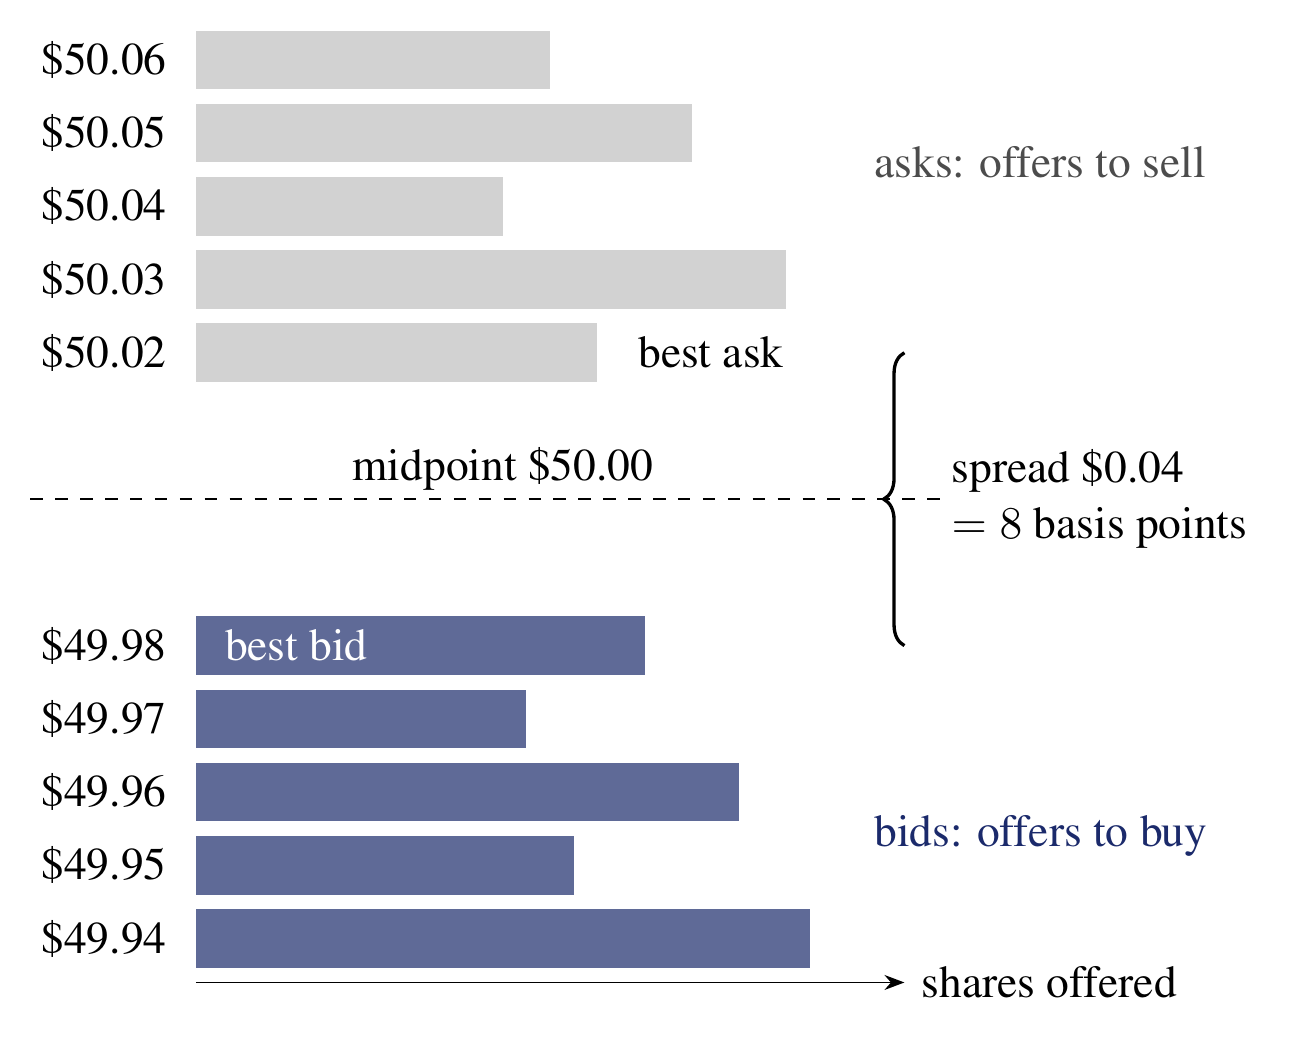
\includegraphics[width=0.8\linewidth]{images/fig06-1-order-book.png}
%\caption{A limit order book. Sellers' asks sit above the midpoint and buyers' bids below it. A buyer who wants to trade at once pays the best ask, \$50.02; a seller receives the best bid, \$49.98. The gap of \$0.04, 8 basis points of the \$50.00 midpoint, is the bid--ask spread.}
%\label{fig:17-book}
%\end{figure}

\subsection{Market and limit orders}

There are two basic ways to trade.

\begin{itemize}
  \item A \textbf{market order}\index{market order|textbf} trades immediately against the best available quotes: a buyer pays the ask, a seller receives the bid. Market orders \emph{demand} liquidity\index{liquidity} and pay the spread.
  \item A \textbf{limit order}\index{limit order|textbf} sets a price and waits in the book until someone trades against it. Limit orders \emph{supply} liquidity and may earn the spread, but risk not being filled, or being filled just before the price moves against them.
\end{itemize}

Large orders are usually broken into many small ones and executed over hours or days to limit their effect on prices.

\subsection{Who provides liquidity}

\textbf{Market makers}\index{market maker|textbf} and high-frequency traders post bids and asks continuously and earn the spread. In return they bear \textbf{inventory risk}, the risk that prices move while they hold shares they have bought but not yet sold, and the risk of trading with better-informed investors. Spreads are wider for small, volatile and thinly traded stocks because these risks are larger there.

\subsection{Long and short positions}

A \textbf{long} position owns a security and gains when its price rises. A \textbf{short} position borrows shares, sells them, and later buys them back to return them, so it gains when the price falls. The short seller pays any dividends to the lender. It also posts \textbf{collateral}\index{collateral|textbf}, cash or securities held as security for the loan, and pays a \textbf{borrowing fee}\index{borrowing fee|textbf} set in the securities-lending market. Most large stocks are cheap to borrow. A minority are hard to borrow and expensive. The lender can also \textbf{recall} the loan, which forces the short seller to buy the shares back.

\subsection{Long--short portfolios}

Academic factors such as HML\index{factor!HML (value)}, introduced in Section~\ref{sec:04-factors}, are \textbf{zero-investment} portfolios. They hold one dollar long and one dollar short, so the proceeds of the short sale pay for the long side. A factor's ``return'' is therefore the difference between the two sides, not a return on capital invested. A real long--short fund must hold collateral and capital against both sides, and it quotes its returns relative to that capital.

\subsection{Turnover}

\textbf{Turnover}\index{turnover|textbf} measures how much of a portfolio is traded in a period. A one-sided\index{hypothesis testing!one-sided and two-sided} monthly turnover of 10\% means that a tenth of the portfolio is sold, and replaced, each month. Turnover multiplies every cost of trading: a strategy that replaces its whole portfolio every month pays its trading costs twelve times a year on each side.

\textbf{Worked example.} A stock is quoted at \$49.98 bid and \$50.02 ask. The midpoint is \$50.00 and the spread is \$0.04, or $0.04/50 = 0.0008$, 8 basis points. Buying with a market order and immediately selling would lose 8 basis points; the one-way cost\index{transaction costs!one-way and round-trip}, half the spread, is 4 basis points.


\section{Paper returns versus implementable returns}
\label{sec:17-paper}

The factor returns in the Kenneth French Data Library\index{Kenneth French data library}, like most portfolio returns in academic research, are \textbf{paper returns}\index{return!paper versus implementable|textbf}. Each month the portfolio is rebuilt from the latest sorts, at closing prices, with no charge for trading. The construction is deliberately simple and transparent, which is why the data is so useful. But it answers the question ``what pattern exists in returns?'' rather than ``what could an investor have earned?''

An \textbf{implementable return}, one an investor could actually have earned, differs in four ways:

\begin{enumerate}
  \item \textbf{Trading costs.}\index{transaction costs|textbf} Every purchase pays above the midpoint price and every sale receives below it; large orders also move the price.
  \item \textbf{Short-selling costs and limits.} Selling short requires borrowing shares, which costs a fee, may be impossible for some stocks, and can be recalled.
  \item \textbf{Timing and execution.} Signals computed from closing prices cannot be traded at those same prices. Orders take time to work, and fast-moving signals lose value while they wait.
  \item \textbf{Scale.} A strategy that works with \$10 million may not work with \$10 billion, because the trades themselves change prices.
\end{enumerate}

None of these makes a paper return wrong. A pattern that cannot be traded profitably may still tell us something about risk or about how prices form. But a claim about profits needs an implementable return, and the two can differ by more than the whole premium.

The gap is largest for strategies that trade often, in small or illiquid stocks, or on the short side. It is smallest for slow strategies in large stocks, which is one reason the market portfolio itself is so hard to beat after costs: it barely trades at all.

\section{The anatomy of trading costs}
\label{sec:17-anatomy}

The cost of a trade has several parts, and they behave differently.

\begin{center}
\small
\begin{tabularx}{0.9\linewidth}{@{}>{\raggedright\arraybackslash}p{0.19\linewidth}>{\raggedright\arraybackslash}X>{\raggedright\arraybackslash}p{0.32\linewidth}@{}}
\toprule
Component & What it is & How it scales \\
\midrule
Commissions and fees & Payments to brokers and exchanges & Small for institutions today; roughly proportional to the amount traded \\
Bid--ask spread & Buying at the ask and selling at the bid, above and below the midpoint & Proportional to the amount traded; wider for small, volatile and illiquid stocks \\
Market impact & The price moving against an order while it is executed, because the order itself carries information or demands liquidity & Grows faster than the trade: roughly with the square root of the order's size relative to volume \\
Delay and opportunity cost & Prices moving before the order is filled, or trades not made at all & Largest for fast signals \\
Short-selling costs & Fees to borrow shares, the risk of recall, rules that restrict shorting & Mostly small, very large for a minority of stocks \\
\bottomrule
\end{tabularx}
\end{center}

The unit used throughout this chapter is the \textbf{one-way cost}\index{transaction costs!one-way and round-trip|textbf}: the cost of buying, or of selling, one dollar of stock, as a fraction of the dollar. For a small trade it is roughly half the bid--ask spread plus commissions. A \textbf{round trip}, buying and later selling, costs twice the one-way cost.

\textbf{Costs have fallen, unevenly.} U.S. stock spreads narrowed sharply in 2001, when prices moved from fractions of a dollar to cents, a change called \textbf{decimalization}\index{decimalization|textbf}, and again as electronic trading spread. Large stocks now trade at spreads of a few basis points, but small, illiquid stocks still cost far more. This matters when reading long histories. A strategy tested from 1963 faced costs in its early decades several times higher than today's. Charging today's costs over the whole history therefore flatters the past, while charging the past's costs today understates what is now possible.

\textbf{Short selling.}\index{short selling|textbf} A short seller borrows shares and pays the lender a fee. Using records from a large lender of shares, D'Avolio (2002) found that most U.S. stocks were cheap to borrow, but that a small group of ``special'' stocks carried high fees, and that these were often the very stocks with the strongest signals to sell short. The lender can also recall the shares at an awkward time, and regulators can ban short selling outright, as the U.S. Securities and Exchange Commission did for financial stocks in September 2008. Miller (1977) argued that when pessimists cannot sell short, prices reflect only the optimists' views, so overpricing can last. If so, anomalies should earn their profits mainly from overpriced stocks, and Stambaugh\index{Stambaugh bias}, Yu and Yuan (2012) found that many anomalies\index{anomaly} earn most of their profits on the short side, exactly where these obstacles bite. A long--short paper portfolio that ignores them overstates what an investor can achieve, sometimes by most of the premium.

The lab uses a single one-way cost and a single borrowing fee for transparency. Real costs vary across stocks and over time, and Section~\ref{sec:17-measuring} shows how they can be estimated.


\section{Measuring costs from public data}
\label{sec:17-measuring}

The best measure of trading costs is a trader's own record. \textbf{Implementation shortfall}\index{implementation shortfall|textbf} (Perold 1988) compares the value of a paper portfolio at the prices when the decision was made with the value of the portfolio actually achieved, capturing spreads, impact, delay and trades never completed. Most researchers do not have such records, so the field relies on estimates.

\textbf{From quotes and trades.} With intraday data, such as the TAQ (Trade and Quote) database of every U.S. trade and quote, two spreads can be measured:

\begin{itemize}
  \item the \textbf{quoted spread}\index{bid--ask spread!quoted|textbf}, the gap between the best bid and ask;
  \item the \textbf{effective spread}\index{bid--ask spread!effective|textbf}, twice the difference between the trade price and the midpoint at the time of the trade.
\end{itemize}

Effective spreads are usually smaller than quoted ones, because many trades execute inside the quotes.

Researchers without intraday data can still estimate spreads from daily prices, which reach back to the 1920s. The shaded box lists the standard methods.

\begin{technote}
\textbf{Technical note: estimating spreads from daily data.} Several estimators infer spreads from daily prices alone, which makes them available back to the 1920s:

\begin{itemize}
  \item \textbf{Roll (1984)}\index{bid--ask spread!estimators|textbf} infers the spread from \textbf{bid--ask bounce}\index{bid--ask bounce|textbf}: because trades alternate randomly between the bid and the ask, successive price changes are negatively correlated, and the size of that correlation\index{correlation} reveals the spread.
  \item \textbf{Hasbrouck (2009)} estimates a similar model with a Bayesian Gibbs sampler, a simulation-based estimation method, which is more robust when the Roll estimator fails.
  \item \textbf{Corwin and Schultz (2012)} use daily high and low prices: highs are usually trades at the ask and lows at the bid, and the spread's share of the range can be separated from volatility\index{volatility} by comparing one-day and two-day ranges.
  \item \textbf{Abdi and Ranaldo (2017)} combine closing, high and low prices for a more precise estimator.
  \item \textbf{Amihud (2002)}\index{illiquidity|textbf} measures \textbf{illiquidity} as the average absolute return per dollar of volume: a measure of price impact rather than a spread.
\end{itemize}

These estimators are noisy for any one stock and month, but useful averaged across portfolios, which is how Novy-Marx and Velikov (2016) used them to estimate the costs of dozens of anomalies.
\end{technote}

\textbf{Estimates from practice.} Frazzini, Israel and Moskowitz (2018) studied \$1.7 trillion of actual trades by a large institutional manager, across 21 developed markets over 19 years. They found trading costs about ten times smaller than earlier academic estimates suggested. The result shows that costs depend on who is trading and how. A patient institution that supplies liquidity pays far less than the typical investor assumed by spread estimators. The evidence, however, comes from a single manager using its own trading methods.

The practical consequence is that a cost assumption is a judgment. A careful study reports results across a range of costs, and the lab does so, from zero to 100 basis points one way.

\section{Turnover, net returns and break-even costs}
\label{sec:17-turnover}

\textbf{Turnover}\index{turnover|textbf} measures how much a portfolio trades. One-sided monthly turnover is the share of the portfolio sold, and replaced, each month. It equals half the sum of the absolute changes in portfolio weights. The changes are measured against the weights the portfolio would have drifted to if it had not traded. A value-weighted\index{index weighting!value-weighted} portfolio whose members never change has zero turnover, however much its prices move.

What drives turnover is how fast the signal changes relative to how often the portfolio is rebuilt:

\begin{itemize}
  \item \textbf{Value} sorts on book-to-market\index{book-to-market ratio} once a year. Book-to-market ratios are persistent, so most stocks stay on the same side from one year to the next.
  \item \textbf{Momentum}\index{momentum|textbf} sorts monthly on the return from 12 months to 2 months ago. Each month's window shares ten of its eleven months with the last one, but enough stocks cross the \textbf{breakpoints}, the cut-offs between groups, to replace about a third of the portfolio each month.
  \item \textbf{Short-term reversal}\index{short-term reversal|textbf} sorts monthly on the previous month's return, which has almost no persistence\index{persistence}. Nearly the whole portfolio is replaced every month.
\end{itemize}

\textbf{From gross to net.} A \textbf{gross} return is before costs; a \textbf{net} return is after them. A long--short portfolio with one dollar on each side and one-sided turnover $T$ sells and buys $T$ on each side, so it trades $4T$ dollars a month. At a one-way cost $c$, its monthly cost and net return are
\begin{equation}
  \text{cost} = 4\,T\,c, \qquad R^{\text{net}}_t = R^{\text{gross}}_t - 4\,T\,c - \frac{\text{borrow fee}}{12}
  \label{eq:17-net}
\end{equation}

The \textbf{break-even cost}\index{transaction costs!break-even|textbf} is the one-way cost at which the average net return is zero:
\begin{equation}
  c^* = \frac{\text{average gross return} - \text{other costs}}{4T}
  \label{eq:17-breakeven}
\end{equation}
It answers the most useful question about a strategy's costs: how cheaply must it trade to be worth trading? For example, a strategy with turnover of 10\% a month that earns 0.4\% a month gross can pay up to $0.4/(4 \times 0.10) = 1\%$ per trade before its profit is gone.

Novy-Marx and Velikov (2016) estimated turnover and costs for value-weighted versions of many anomalies. Their full-sample figures for the three strategies in this chapter (Table 3 of the working-paper version), with break-even costs computed from their gross returns using Equation~\eqref{eq:17-breakeven}:

\begin{center}
\small
\begin{tabularx}{\linewidth}{@{}>{\raggedright\arraybackslash}X>{\raggedright\arraybackslash}p{0.13\linewidth}>{\raggedright\arraybackslash}p{0.13\linewidth}>{\raggedright\arraybackslash}p{0.13\linewidth}>{\raggedright\arraybackslash}p{0.13\linewidth}>{\raggedright\arraybackslash}p{0.12\linewidth}@{}}
\toprule
Strategy & One-sided monthly turnover & Gross return (\% per month) & Estimated cost (\% per month) & Net return (\% per month) & Break-even one-way cost \\
\midrule
Value (book-to-market) & 2.9\% & 0.47 & 0.05 & 0.42 & about 4\% \\
Momentum & 34.5\% & 1.33 & 0.65 & 0.68 & about 1\% \\
Short-term reversal & 90.9\% & 0.37 & 1.65 & $-1.28$ & about 0.1\% \\
\bottomrule
\end{tabularx}
\end{center}

The three strategies differ sharply in how much cost they can bear (Figure~\ref{fig:17-breakeven}). Value could pay several percent per trade and still make a profit. Momentum survives costs of up to about one percent per trade. A careful institution can trade that cheaply, but a careless one may not. Short-term reversal is profitable on paper, but it would need to trade for about ten basis points per trade. That is less than most investors pay for the small, recently volatile stocks it buys and sells. Its paper profit is real, but tiny compared with the trading it needs.

\providecolor{fenavy}{HTML}{1B2A6B}

\begin{figure}[htbp]
  \centering
  \scalebox{0.8}{%
\begin{tikzpicture}[
    % Gross return (% a month) and monthly one-way turnover, from the table.
    % Net return = gross - 4 * turnover * cost; break-even = gross / (4 * turnover).
    declare function={
      valG = 0.47;  valT = 0.029;
      momG = 1.33;  momT = 0.346;
      revG = 0.38;  revT = 0.95;
    }]
  \begin{axis}[
    width=0.61\linewidth, height=0.38\linewidth,
    axis lines=left,
    axis line style={-stealth, thin},
    xmin=0, xmax=1.3, ymin=-1.6, ymax=1.45,
    xtick={0,0.2,0.4,0.6,0.8,1,1.2},
    ytick={-1,0,1},
    xticklabel style={/pgf/number format/fixed},
    xlabel={One-way trading cost (\%)},
    ylabel={Net return (\% a month)},
    clip=false,
  ]
    \addplot[gray!60, thin, domain=0:1.3, samples=2] {0};

    % Value
    \addplot[fenavy, very thick, domain=0:1.3, samples=2] {valG - 4*valT*x};
    % Momentum
    \addplot[thick, dashed, domain=0:1.3, samples=2] {momG - 4*momT*x};
    % Short-term reversal (stops at the bottom of the chart)
    \addplot[very thick, densely dotted, domain=0:0.52, samples=2] {revG - 4*revT*x};

    % Break-even points
    \fill (axis cs:{momG/(4*momT)},0) circle (2.2pt);
    \fill (axis cs:{revG/(4*revT)},0) circle (2.2pt);
    \node[anchor=north east, font=\small] at (axis cs:{momG/(4*momT)-0.02},-0.03)
      {break-even $\approx 1\%$};
    \node[anchor=south west, font=\small] at (axis cs:{revG/(4*revT)+0.03},0.03)
      {$\approx 0.1\%$};

    % Line labels
    \node[fenavy, anchor=west, font=\small] at (axis cs:1.31,{valG-4*valT*1.3+0.05}) {value};
    \node[anchor=west, font=\small] at (axis cs:1.31,{momG-4*momT*1.3}) {momentum};
    \node[anchor=west, font=\small] at (axis cs:0.48,-1.05) {short-term reversal};
  \end{axis}
  \end{tikzpicture}%
}
  \caption{The more a strategy trades, the faster its profit disappears as costs rise. Net return against one-way trading cost, from the turnover and gross
    returns in the table. Each line falls at a rate of four times the strategy's
    turnover; it crosses zero at the break-even cost. Value's line is nearly
    flat and crosses zero off the chart, at about 4\%.}
  \label{fig:17-breakeven}
\end{figure}

%\begin{figure}[htbp]
%\centering
%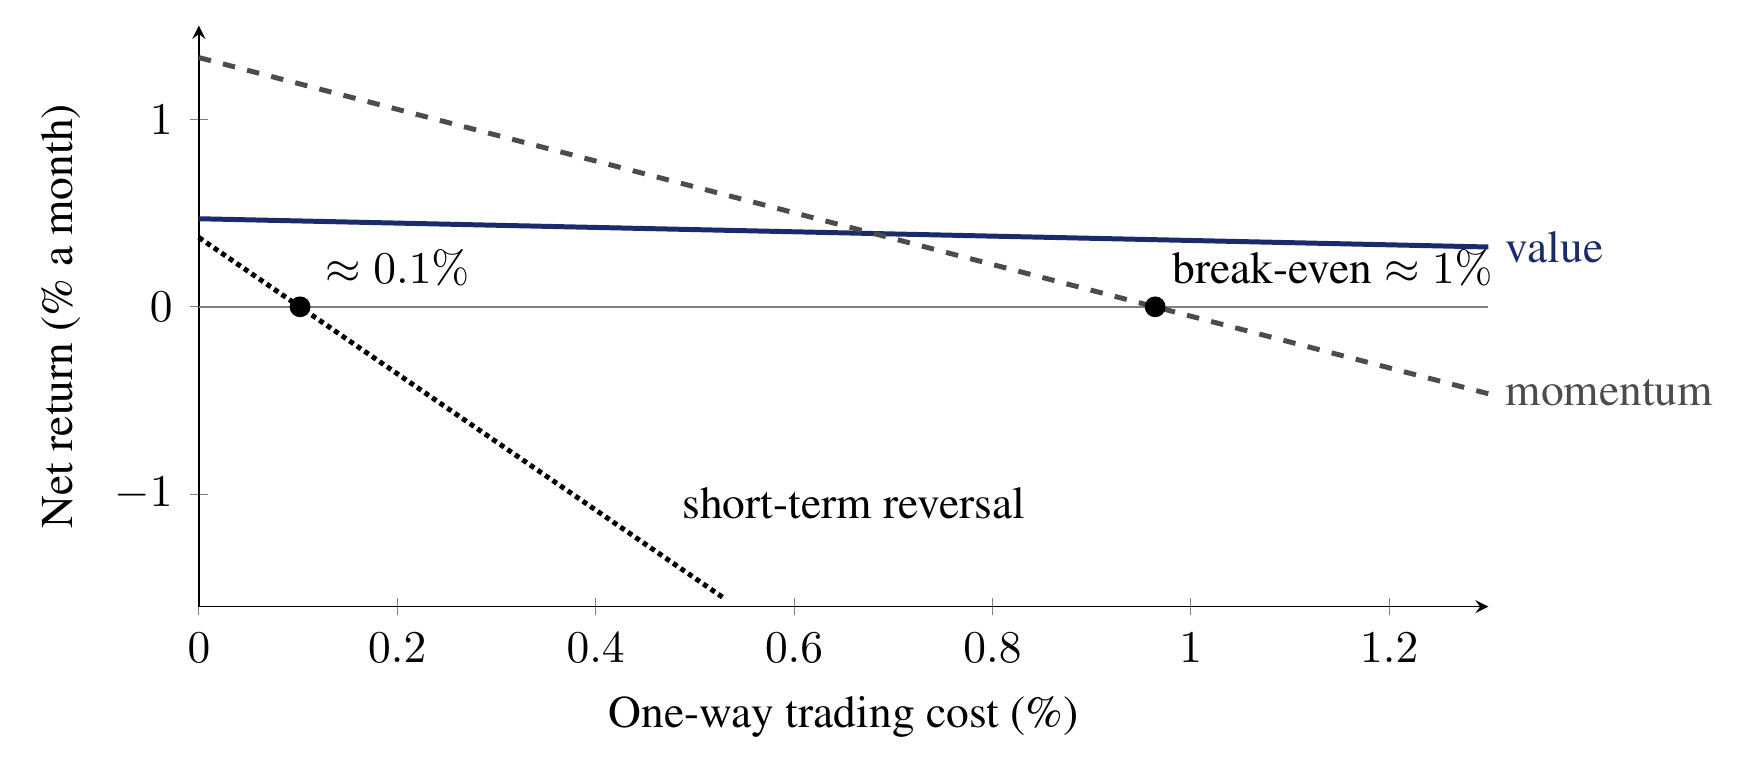
\includegraphics[width=0.85\linewidth]{images/fig06-2-break-even.png}
%\caption{Net return against one-way trading cost, from the turnover and gross returns in the table. Each line falls at a rate of four times the strategy's turnover; it crosses zero at the break-even cost. Value's line is nearly flat and crosses zero off the chart, at about 4\%.}
%\label{fig:17-breakeven}
%\end{figure}

A gross ranking by Sharpe ratio\index{Sharpe ratio} or t-statistic\index{t-statistic} therefore says little about which strategy an investor should prefer. The net ranking depends on turnover as much as on the gross premium.


\section{Market impact and capacity}
\label{sec:17-capacity}

Spreads are roughly a fixed cost per dollar traded. Market impact is not: the more a strategy trades relative to the market's volume, the more each dollar costs. This is what gives every strategy a \textbf{capacity}\index{capacity|textbf}, a size beyond which its net returns shrink toward zero.

\textbf{Why prices move.} Kyle (1985) described market makers who cannot tell orders from well-informed traders apart from other orders, so they move their prices in the direction of every order. Large orders are more likely to carry information and harder to absorb, so they move prices more. Studies of real institutional trades find that the price impact grows roughly with the square root of an order's size relative to the day's trading volume (Almgren, Thum, Hauptmann and Li 2005; T\'oth et al.\ 2011). A common working model is
\begin{equation}
  \text{impact per dollar} \approx Y\,\sigma_{daily}\,\sqrt{\frac{Q}{V}}
  \label{eq:17-impact}
\end{equation}
Here $Q$ is the order size, $V$ is daily volume, $\sigma_{daily}$ is daily volatility and $Y$ is a constant close to one. The ratio $Q/V$ is the \textbf{participation rate}\index{participation rate|textbf}, the order's share of the day's trading. Trading 1\% of a day's volume in a stock with 2\% daily volatility costs about $2\% \times \sqrt{0.01} = 0.2\%$ in impact. Trading 10\% costs about $2\% \times \sqrt{0.10} \approx 0.6\%$ (Figure~\ref{fig:17-impact}).

\providecolor{fenavy}{HTML}{1B2A6B}

\begin{figure}[htbp]
  \centering
  \scalebox{0.8}{%
\begin{tikzpicture}[
    % Impact (%) = Y * sigma * sqrt(Q/V), with Y = 1 and sigma = 2%.
    % x is Q/V in percent, so impact = 2 * sqrt(x/100) = 0.2 * sqrt(x).
    declare function={impact(\x) = 0.2*sqrt(\x);}
  ]
  \begin{axis}[
    width=0.55\linewidth, height=0.35\linewidth,
    axis lines=left,
    axis line style={-stealth, thin},
    xmin=0, xmax=20.5, ymin=0, ymax=1,
    xtick={0,5,...,20},
    ytick={0,0.2,0.4,0.6,0.8,1},
    yticklabel style={/pgf/number format/fixed},
    tick label style={font=\small},
    xlabel={Order size as a share of daily volume, $Q/V$ (\%)},
    ylabel={Impact per dollar (\%)},
    samples=200, domain=0:20,
    clip=false,
  ]
    % If impact were linear (for comparison)
    \addplot[gray!70, densely dashed, thin, samples=2] {0.0215*x};
    \node[gray!40!black, font=\small, anchor=west] at (axis cs:20.2,0.36)
      {if impact were linear};

    % Square-root impact
    \addplot[fenavy, very thick] {impact(x)};
    \node[fenavy, font=\small, anchor=west] at (axis cs:20.2,{impact(20)})
      {square root};

    % Marked points
    \fill[fenavy] (axis cs:1,0.2) circle (2.2pt);
    \draw[gray!50] (axis cs:1.2,0.21) -- (axis cs:4.6,0.34);
    \node[font=\small, anchor=west] at (axis cs:4.6,0.34) {1\% of volume: 0.2\%};

    \fill[fenavy] (axis cs:10,0.632) circle (2.2pt);
    \node[font=\small, anchor=north west] at (axis cs:10.5,0.62)
      {10\% of volume: 0.6\%};
  \end{axis}
  \end{tikzpicture}%
}
  \caption{Bigger orders cost more per dollar, though less than in proportion to their size. Square-root market impact for a stock with 2\% daily volatility,
    from Equation~\eqref{eq:17-impact} with $Y = 1$. Ten times the order size
    costs about three times as much per dollar, not ten times; but total
    impact cost, per dollar times dollars, still rises faster than the order.}
  \label{fig:17-impact}
\end{figure}

%\begin{figure}[htbp]
%\centering
%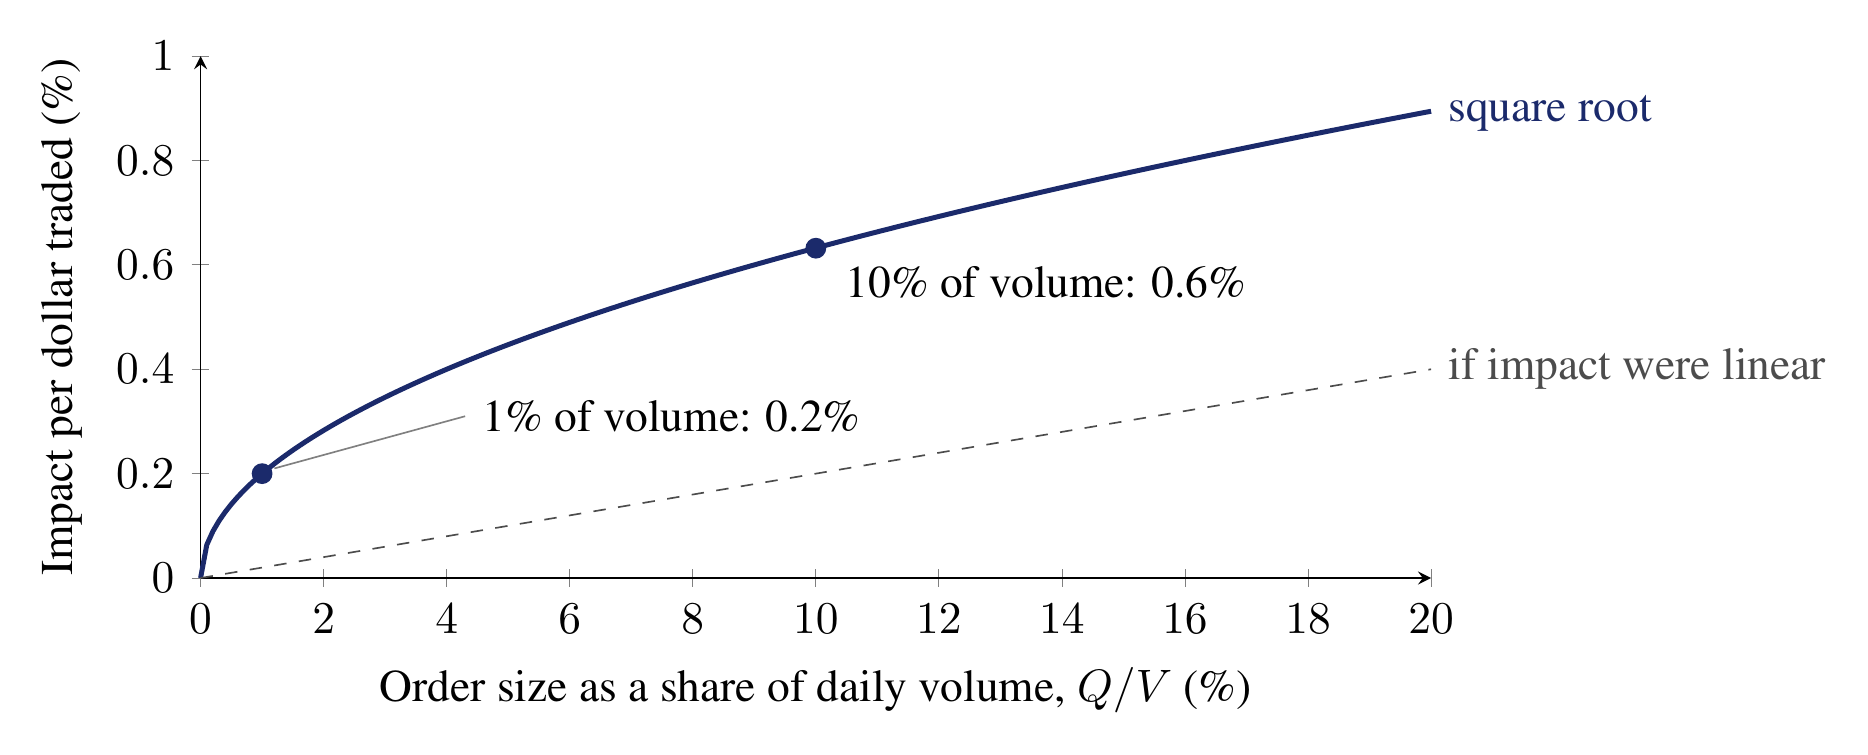
\includegraphics[width=0.85\linewidth]{images/fig06-3-impact.png}
%\caption{Square-root market impact for a stock with 2\% daily volatility, from Equation~\eqref{eq:17-impact} with $Y = 1$. Ten times the order size costs about three times as much per dollar, not ten times; but total impact cost, per dollar times dollars, still rises faster than the order.}
%\label{fig:17-impact}
%\end{figure}

\textbf{From impact to capacity.} A strategy that manages assets $A$ with turnover $T$ trades about $2TA$ on each side every month, spread across its holdings. As $A$ grows, the participation rate $Q/V$ rises. Impact per dollar rises with its square root, so total impact cost rises faster than the assets. Net return therefore falls as the fund grows, slowly at first and then quickly. Capacity can be defined as the size at which the net return is halved, or the size at which it reaches zero. An investor would want to stop well before either point.

Three features\index{features and targets} of a strategy set its capacity:

\begin{enumerate}
  \item \textbf{Turnover.}\index{turnover|textbf} Every dollar not traded is a dollar that does not move prices.
  \item \textbf{Liquidity of its holdings.} Strategies that concentrate in small stocks hit their limits first.
  \item \textbf{Gross premium.} A larger premium can absorb more cost before it is gone.
\end{enumerate}

Capacity also has an industry-wide side. If many managers follow similar signals, their combined trades set the price impact. A strategy's capacity is then shared among everyone who trades it. Berk and Green (2004) argued that in a competitive market, money flows to skilled managers until their returns after costs are no better than the alternatives.

The capacity estimates in this chapter's lab rest on stated assumptions about volume, spreads and the impact constant. They are an illustration of how capacity arises and what it depends on, not a forecast for any real fund.

\section{Designing for costs}
\label{sec:17-design}

A paper portfolio is built as if trading were free, so it trades whenever the signal moves, however slightly. A portfolio designed for costs trades only when the expected gain exceeds the cost. Several simple rules capture most of the benefit.

\begin{itemize}
  \item \textbf{Buy/hold spreads (banding).} Buy a stock only when it enters the top 30\% on the signal, but keep holding it until it falls out of, say, the top 50\%. Stocks that wobble around the breakpoint no longer generate trades. Novy-Marx and Velikov (2016) found this the single most effective simple way to reduce costs.
  \item \textbf{Slower rebalancing\index{rebalancing}.} Rebuilding the portfolio quarterly rather than monthly cuts turnover for slow signals at little cost in signal. For fast signals it gives up most of the premium.
  \item \textbf{Partial trading.} G\^arleanu and Pedersen (2013) showed that with predictable returns\index{return predictability} and \textbf{quadratic trading costs}\index{transaction costs!quadratic|textbf}, costs that rise with the square of the amount traded, the optimal policy trades only part of the way toward the target each period, and aims at a target that anticipates where the signal is heading.
  \item \textbf{Netting and combining signals.} A multi-signal portfolio can cross trades internally: a stock that momentum wants to sell and value wants to buy need not be traded at all.
  \item \textbf{Liquidity screens.}\index{liquidity|textbf} Restricting the universe to larger, more liquid stocks raises capacity and lowers costs, usually at some cost in gross premium, since many anomalies are strongest in small stocks.
\end{itemize}

Each rule trades a little signal for a lot less trading. The trade-off depends on how fast the signal decays: banding costs little for momentum, whose ranks change gradually, and cannot rescue short-term reversal, whose signal is gone within a month.

\textbf{Saving costs is also a search.} Every design choice, such as the width of a band, how often to rebalance or which stocks to exclude, can be tuned to make a backtest look better, so the warnings about selection and overfitting\index{overfitting} in Section~\ref{sec:01-backtests} apply in full. Chen and Velikov (2023) studied 204 anomalies, allowing for effective spreads, the decline in returns after publication\index{anomaly!post-publication decay} and modern trading technology. They found that the average anomaly's expected return, net of these effects, was about 4 basis points a month. Strategies that looked impressive after costs in their own samples, once cost-saving rules were added, did not escape that conclusion. A cost-saving design should therefore be fixed in advance and judged out of sample, like any other part of a strategy.


\begin{callout}
\textbf{What Failed: buying last month's losers.} Jegadeesh (1990) and Lehmann (1990) showed that stocks with low returns over the past week or month tended to rebound, and stocks with high returns tended to fall back. On paper the pattern is strong and statistically robust, and the Fama--French\index{Fama--French factors} short-term reversal factor still has a positive average return. The trouble is trading. The strategy replaces almost its whole portfolio every month. It buys and sells stocks that have just moved sharply, often small and illiquid ones, where spreads are widest. Novy-Marx and Velikov (2016) estimated that its costs were larger than its gross return by more than a percentage point a month. Nagel (2012) argued that much of the reversal is a reward for supplying liquidity to impatient traders. That reward goes to market makers, who trade cheaply, not to investors who must pay the spread. For an ordinary investor, the claim that buying recent losers is profitable \textbf{fails} once costs are counted.
\end{callout}

\section{Lab~\thechapter: Replicating Novy-Marx and Velikov (2016)}
\label{sec:17-lab}

\begin{callout}
\textbf{Lab~\ref{ch:13} at a glance.} \emph{Papers replicated:} Novy-Marx and Velikov (2016); a capacity analysis in the spirit of Frazzini, Israel and Moskowitz (2018). All data are free. \emph{Claim on trial:} a strategy that is profitable in a backtest is profitable to trade. \emph{Data:} three long--short factors from the Kenneth R. French Data Library, value (HML), momentum (Mom) and short-term reversal (ST Rev), from July 1963, plus a simulated stock universe. \emph{Run time:} a few seconds. \emph{Code:} repository folder \texttt{ch05-costs/}, with a guided notebook.
\end{callout}

The lab takes the three factors and asks what each would have earned after costs.

\textbf{Part A: gross performance.} The lab reports average returns, t-statistics and Sharpe ratios as published. On paper, all three look like discoveries.

\textbf{Part B: turnover.} The French library does not publish holdings, so turnover comes from Novy-Marx and Velikov's estimates and from a simulated universe of 1,000 stocks over 40 years, with fat tails\index{fat tails}, realistic company sizes, and value-weighted 30/70 sorts built like the Fama--French factors (value updated each June, momentum and reversal each month). With no delistings\index{delisting} or new listings, its turnover is a lower bound: about 2\% a month for value, 25\% for momentum and 76\% for reversal, close to the published estimates. Turnover follows mechanically from how each signal is built.

\textbf{Part C: costs.} The lab computes net returns for one-way costs from 0 to 100 basis points plus a short-borrowing fee of 0.25\% a year, the break-even costs, and the Sharpe-ratio ranking before and after a headline cost of 20 basis points. Lab Figure~\ref{ch:13}.1 plots net return against cost with each break-even point marked, and Lab Figure~\ref{ch:13}.2 shows the growth of a dollar on paper and after costs.

\textbf{Part D: capacity.} The simulated universe is scaled to a \$50 trillion market, with daily volume of 0.4\% of each company's value, half-spreads from 2 to 50 basis points, and square-root impact, and each strategy's net return is traced as its assets grow from \$10 million to \$1 trillion. The assumptions are explicit and adjustable.

\textbf{Part E: mitigation, with known truth.} Because expected returns are known in the simulated universe, the lab compares the standard sort with buy/hold spreads of increasing width without sampling noise. For momentum at a one-way cost of 50 basis points, holding stocks until they leave the top 50\% cuts turnover roughly in half, from about 25\% to 12\% a month, gives up about a fifth of the expected gross return, and raises the expected net return from about 0.30\% to 0.41\% a month. For reversal, no band width rescues the strategy at that cost: the signal decays too fast for patience to pay.

The README in \texttt{ch05-costs} records what has been tested, including that the parsers for the momentum and reversal files have been tested on the library's layout but not yet on the live files.

\subsection*{Your verdict}

Reach your own verdict on the claim from the numbers in your own run, using the scale of Section~\ref{sec:01-method}. Then compare it with the published evidence summarized in Section~\ref{sec:17-verdict}. If your verdict differs, explain which of your results led you there.

\section{Where the evidence stands}
\label{sec:17-verdict}

The published studies point to a clear pattern: \textbf{whether a profitable backtest is profitable to trade depends on how much the strategy trades, what it trades and how much money is behind it: slow strategies in liquid stocks survive realistic costs, while fast strategies in small stocks often do not.} The table summarizes the evidence as of November 2026. The lab lets you check it with free data.

{\small
\begin{longtable}{@{}>{\raggedright\arraybackslash}p{0.19\linewidth}>{\raggedright\arraybackslash}p{0.13\linewidth}>{\raggedright\arraybackslash}p{\dimexpr 0.45\linewidth-6\tabcolsep\relax}>{\raggedright\arraybackslash}p{0.23\linewidth}@{}}
\toprule
Situation & Holds? & Why & Evidence \\
\midrule
\endfirsthead
\multicolumn{4}{@{}l}{\emph{(continued)}} \\
\toprule
Situation & Holds? & Why & Evidence \\
\midrule
\endhead
\midrule
\multicolumn{4}{r@{}}{\emph{(continued on the next page)}} \\
\endfoot
\bottomrule
\endlastfoot
Slow strategies, such as value & \textbf{Yes} & Turnover of about 3\% a month gives a break-even cost of about 4\% per trade. & Novy-Marx and Velikov (2016) \\
\addlinespace[3pt]
Momentum & \textbf{Partly} & Survives one-way costs up to about 1\%, but its profits concentrate in costly stocks and shrink with size. & Novy-Marx and Velikov (2016); Lesmond, Schill and Zhou (2004); Korajczyk and Sadka (2004) \\
\addlinespace[3pt]
Short-term reversal & \textbf{No} & Nearly full monthly turnover; costs exceed its gross return by more than a point a month. & Novy-Marx and Velikov (2016) \\
\addlinespace[3pt]
High-turnover strategies in general & \textbf{No} & Most strategies trading over half their portfolio monthly lose significance after costs. & Novy-Marx and Velikov (2016) \\
\addlinespace[3pt]
For a large, patient institution & \textbf{More often} & Actual costs were an order of magnitude below academic estimates, but from one manager's trades. & Frazzini, Israel and Moskowitz (2018) \\
\addlinespace[3pt]
Strategies that rely on the short side & \textbf{Often not} & Many anomalies earn most on the short side, where fees, recalls and bans bite. & D'Avolio (2002); Stambaugh, Yu and Yuan (2012) \\
\addlinespace[3pt]
The average anomaly & \textbf{No} & After costs and post-publication decay, its expected return is about 4 basis points a month. & Chen and Velikov (2023) \\
\end{longtable}
}

The claim holds only for strategies whose break-even costs sit well above what their investors actually pay, at the size they intend to run.

\textbf{What would change the picture.} The claim would gain support if many managers' trading records confirmed costs as low as those of Frazzini, Israel and Moskowitz (2018), and lose it if cost-saving designs fixed in advance failed out of sample.

\section{What practitioners and investors can use}
\label{sec:17-investors}

Five questions turn the evidence in Section~\ref{sec:17-verdict} into a checklist for any strategy an investor is shown:

\begin{enumerate}
  \item \textbf{What is the turnover?} Ask for one-sided monthly turnover on both sides. If it is not known, the strategy has not been evaluated as an investment.
  \item \textbf{What is the break-even cost, and what will you pay?} A strategy that needs costs below ten basis points is a bet on execution, not on the signal.
  \item \textbf{What does the short side cost?} Ask how much return comes from it, what borrowing fees were assumed, and what happens if hard-to-borrow stocks cannot be shorted.
  \item \textbf{At what size?} Ask for net returns at the planned assets and how market impact was estimated. Capacity claims without stated assumptions are marketing.
  \item \textbf{Were cost-saving rules chosen in advance?} Bands, rebalancing schedules and liquidity screens are parameters too. Ask whether they were fixed before the backtest.
\end{enumerate}

Costs change the ranking of strategies, not just their level: a modest, slow premium harvested cheaply may be worth more than a spectacular, fast one that cannot be. Chapters~\ref{ch:14} and~\ref{ch:15} test more anomalies, and report their evidence after costs as well as before.
   % trading costs
% Chapter 18 -- Claim: Low-Risk Stocks Beat High-Risk Stocks
% Requires: amsmath, amssymb, booktabs, array, tabularx, longtable, graphicx, tcolorbox (breakable, skins), hyperref or url.
% Defines the callout box only if the preamble has not.
\providecolor{fenavy}{HTML}{1B2A6B}
\providecolor{feshade}{HTML}{F3F5FA}
\makeatletter
\@ifundefined{callout}{%
  \newtcolorbox{callout}{breakable, enhanced,
    colback=white, colframe=gray!70, boxrule=0.5pt, arc=1mm,
    borderline west={2.5pt}{0pt}{gray!70},
    left=8pt, right=8pt, top=4pt, bottom=4pt}%
}{}
\makeatother

\providecolor{fenavy}{HTML}{1B2A6B}
\providecolor{feshade}{HTML}{F3F5FA}
\makeatletter
% Shaded box for optional technical material that general readers may skip.
\@ifundefined{technote}{%
  \newtcolorbox{technote}{breakable, enhanced,
    colback=feshade, colframe=fenavy!60, boxrule=0.5pt, arc=1mm,
    left=8pt, right=8pt, top=4pt, bottom=4pt}%
}{}
\makeatother

\chapter{Claim: Low-Risk Stocks Beat High-Risk Stocks}
\label{ch:14}

Common sense says that riskier investments must pay more on average, or no one would hold them. Yet investors who bought the dull, steady stocks of the market, such as utilities and grocery chains, have historically done about as well as those who bought the most exciting ones, with far smaller swings along the way. This chapter asks whether that pattern is real, why it might exist, and whether an investor can profit from it.

The capital asset pricing model\index{capital asset pricing model (CAPM)} makes one central prediction: assets that move more with the market should earn more. If a stock's beta\index{beta} doubles, its expected excess return\index{return!excess} should double too. This was among the first predictions in finance to be tested, and Chapter~\ref{ch:03} showed that it failed early. Black, Jensen and Scholes (1972) and Fama and MacBeth (1973), who estimated the link between returns and beta month by month and averaged the results, found that average returns did rise with beta, but far less steeply than the theory implied. Black (1972) offered an explanation based on limits to borrowing. Some investors want more risk but cannot borrow freely. Instead of borrowing, they buy high-beta stocks, which pushes up their prices and lowers their later returns.

For two decades the flat security market line was treated as a curiosity. It became a claim about profits when later research made the effect larger and easier to trade. Ang, Hodrick, Xing and Zhang (2006) tested the theory that only market risk is priced, and found that stocks with high idiosyncratic volatility\index{volatility}, the part of volatility not explained by the market, earned strikingly low returns. Asking why professionals did not trade such mispricing away, Baker, Bradley and Wurgler (2011) argued that fund managers judged against a benchmark have little reason to correct the mispricing. To show that the pattern reflects limits on borrowing everywhere, not a quirk of U.S. stocks, Frazzini and Pedersen (2014) built a leveraged ``betting-against-beta'' factor that earned high risk-adjusted returns in many countries and asset classes. The pattern is now called the \textbf{low-risk anomaly}\index{low-risk anomaly|textbf}. Novy-Marx and Velikov (2022) later argued that much of the betting-against-beta performance comes from the way the factor is built, not from low risk itself.

The question matters in practice. Low-volatility funds grew rapidly after 2010, and companies still use beta to set the return a new project must earn. The anomaly is also hard to exploit, because exploiting it needs leverage, which is exactly what the explanation says investors avoid. The claim on trial\index{claims-on-trial method} is: \textbf{low-beta and low-volatility stocks earn higher risk-adjusted returns than high-risk stocks, and a leveraged long--short portfolio captures the difference.}

The lab in Section~\ref{sec:18-lab} repeats two classic tests on the free beta- and variance-sorted portfolios of the Kenneth R. French Data Library: the security market line of Black, Jensen and Scholes (1972) and the cross-sectional regressions of Fama and MacBeth (1973). It then rebuilds the betting-against-beta factor of Frazzini and Pedersen (2014) and compares it with AQR's free published series. The goal is to check whether low-risk stocks still earn more than the CAPM predicts once costs and construction choices are taken into account.

By the end of the chapter you will be able to:

\begin{itemize}
  \item estimate a beta, split total risk\index{risk!total} into systematic and idiosyncratic parts, and compute a CAPM alpha\index{alpha};
  \item draw the security market line\index{security market line}, and explain how limits on leverage\index{leverage} flatten it;
  \item build a beta-neutral\index{market-neutral} betting-against-beta\index{betting against beta (BAB)} portfolio, and compare the explanations for the anomaly, such as leverage limits and lottery preferences\index{lottery preference};
  \item judge whether a minimum-volatility or BAB fund can deliver what its backtest\index{backtest} promises.
\end{itemize}


\section{Foundations: beta, the CAPM and the security market line}
\label{sec:18-foundations}

\subsection{Beta, the CAPM and the security market line}

Chapter~\ref{ch:03} introduced beta, the CAPM and the security market line (Section~\ref{sec:04-capm}). Beta is the slope of a regression of an asset's excess return on the market's excess return (Equation~\eqref{eq:04-capm}). The market itself has a beta of 1. The CAPM says that expected excess returns rise in a straight line with beta. Two consequences of the model matter for this chapter.

First, the security market line passes through the risk-free rate\index{risk-free rate} at $\beta = 0$ and through the market at $\beta = 1$, so its slope equals the market premium.

Second, an asset's \textbf{total risk}\index{risk!total|textbf}, the variance\index{variance} of its return, splits into two parts. The systematic part is $\beta_i^2\,\mathrm{Var}(R_m)$. The idiosyncratic part is the variance of the regression residual\index{regression!residuals}. Only the systematic part earns a reward, because investors can diversify\index{diversification} the idiosyncratic part away at no cost. Two stocks with the same volatility can therefore have very different betas, and the CAPM says they should have very different expected returns\index{return!expected}.

\subsection{Alpha}

An asset's alpha, often called Jensen's alpha, is the intercept of the same regression: the average return beyond what beta explains (Section~\ref{sec:04-capm}). Under the CAPM every alpha is zero. A multifactor alpha adds other factors to the regression, such as size, value and momentum\index{momentum} (Chapter~\ref{ch:03}). The low-risk anomaly is a claim about how alpha varies with beta: low-beta stocks have had positive alphas and high-beta stocks negative ones.

The CAPM assumes that investors can borrow and lend freely at the risk-free rate. An investor who wants more risk than the market can then borrow and buy more of the market. Many investors cannot do this. Mutual funds and pension plans face limits on \textbf{leverage}\index{leverage|textbf}, which means borrowing to hold more than their capital. Individuals face \textbf{margin} requirements and pay more than the risk-free rate to borrow. Black (1972) showed that without riskless borrowing the SML is still a straight line, but a flatter one. It starts at the return on a \textbf{zero-beta portfolio}\index{zero-beta portfolio|textbf}, a portfolio uncorrelated with the market, whose return lies above the risk-free rate.

\textbf{Worked example.} The risk-free rate is 3\% and the market premium is 6\% (Figure~\ref{fig:18-sml}).

\begin{itemize}
  \item Stock A has a beta of 0.6 and has averaged 9\%. The CAPM predicts $3\% + 0.6 \times 6\% = 6.6\%$, so A's alpha is $+2.4\%$.
  \item Stock B has a beta of 1.5 and has averaged 10\%. The CAPM predicts $3\% + 1.5 \times 6\% = 12\%$, so B's alpha is $-2\%$.
  \item An investor who can borrow at 3\% can lever A to a beta of 1. She holds $1/0.6 = 1.67$ dollars of A for each dollar of capital and borrows the remaining 0.67 dollars. Her expected return is $3\% + 1.67 \times (9\% - 3\%) = 13\%$, compared with 9\% for the market at the same beta. Even at a borrowing rate of 5\%, she earns $1.67 \times 9\% - 0.67 \times 5\% \approx 11.7\%$.
  \item An investor who cannot borrow and wants a beta above 1 must buy B instead. If many investors are in that position, they bid up high-beta stocks such as B and push down their future returns. That is the core of the leverage-constraint explanation in Section~\ref{sec:18-explanations}.
\end{itemize}

\begin{figure}[htbp]
\centering
\scalebox{0.8}{%
\begin{tikzpicture}[
  % CAPM: r = 3 + 6 * beta. A = (0.6, 9), B = (1.5, 10); the line through A and B
  declare function={capm(\b) = 3 + 6*\b;  flat(\b) = 9 + (\b - 0.6)/0.9;}
]
\begin{axis}[
  width=0.6\linewidth, height=0.34\linewidth,
  axis lines=left, axis line style={-stealth},
  xmin=0, xmax=2, ymin=0, ymax=15.5,
  xtick={0,0.5,...,2}, ytick={0,5,10,15},
  xticklabel style={/pgf/number format/fixed},
  xlabel={Beta}, ylabel={Average return (\%)},
  clip=false,
]
  \addplot[fegray, thick, dashed, domain=0:2, samples=2] {flat(x)};
  \addplot[fenavy, very thick, domain=0:2, samples=2] {capm(x)};
  \fill (axis cs:0.6,9)  circle (2.6pt);
  \fill (axis cs:1,9)    circle (2.6pt);
  \fill (axis cs:1.5,10) circle (2.6pt);
  \node[anchor=south] at (axis cs:0.6,9.5) {A: $\alpha = +2.4\%$};
  \node[anchor=north west] at (axis cs:0.98,8.4) {market};
  \node[anchor=north west] at (axis cs:1.47,9.1) {B: $\alpha = -2\%$};
  \node[anchor=north west] at (axis cs:0.02,2.7) {$r_f = 3\%$};
  \node[fenavy, anchor=west] at (axis cs:2.02,15) {CAPM line};
  \node[fegray, anchor=west, align=left] at (axis cs:2.02,{flat(2)})
    {line through\\A and B};
\end{axis}
\end{tikzpicture}%
}
\caption{Low-beta stocks have done better, and high-beta stocks worse, than the CAPM predicts. The security market line in the worked example. The CAPM line runs from the risk-free rate of 3\% through the market at a beta of 1. Stock A lies above it (positive alpha) and stock B below it (negative alpha), so the line through A and B is flatter than the CAPM predicts.}
\label{fig:18-sml}
\end{figure}

\section{How it works}
\label{sec:18-how}

There are three ways to sort stocks on risk, and the literature uses all three.

\begin{itemize}
  \item \textbf{Beta.}\index{beta|textbf} Estimate each stock's beta from past returns, typically 36 to 60 months of monthly data or a year of daily data. Sort into portfolios. This tests the CAPM directly.
  \item \textbf{Total volatility.} Sort on the standard deviation\index{standard deviation} of past daily returns, often over one to three months. This needs no market model, and it is how most low-volatility funds work.
  \item \textbf{Idiosyncratic volatility.}\index{idiosyncratic volatility|textbf} Sort on the volatility of residuals from a factor model\index{factor model}, usually the Fama--French\index{Fama--French factors} three-factor model. Under the CAPM this risk should not be priced at all, so a negative relation is especially puzzling.
\end{itemize}

The three measures are strongly correlated. High-beta stocks tend to be volatile, and volatile stocks tend to have high idiosyncratic risk\index{risk!idiosyncratic}. Separating them is one of the open problems in this chapter.

A flat SML shows up in two ways. The first is in \emph{alphas}: low-risk portfolios have positive CAPM alphas, and high-risk portfolios negative ones. The second is in a \emph{long-short portfolio\index{long--short portfolio}}. The simple version buys low-risk stocks and sells high-risk stocks short. It has a strongly negative beta, so it loses money in rising markets even when the SML is flat. Its average return can be negative while its alpha is positive. \textbf{Betting against beta (BAB)}\index{betting against beta (BAB)|textbf} fixes this. It levers the low-beta leg up to a beta of 1 and scales the high-beta leg down to a beta of 1. The portfolio is then \textbf{beta-neutral}\index{market-neutral|textbf}, with no net exposure to the market (Figure~\ref{fig:18-bab}). The shaded box gives the formula.

\begin{technote}
\textbf{Technical note: the BAB return.} In symbols, the portfolio's excess return is
\begin{equation}
  r_{\mathrm{BAB}} = \frac{r_L - r_f}{\beta_L} - \frac{r_H - r_f}{\beta_H}
  \label{eq:18-bab}
\end{equation}
If the SML is flat, this portfolio earns a positive return with no market exposure. The betas must be \textbf{ex ante}, estimated from data available when the portfolio is formed. Otherwise the construction looks ahead (Section~\ref{sec:02-lookahead}).
\end{technote}

\begin{figure}[htbp]
\centering
\scalebox{0.8}{%
\begin{tikzpicture}
\begin{axis}[
  width=0.6\linewidth, height=0.34\linewidth,
  ybar, bar width=0.6cm,
  axis lines=left, axis line style={-stealth},
  ymin=-2, ymax=2.2, ytick={-2,-1,0,1,2},
  ylabel={Dollars per \$1 of capital},
  symbolic x coords={L,H}, xtick=data,
  xticklabels={{Low-beta leg\\($\beta_L = 0.6$)}, {High-beta leg\\($\beta_H = 1.5$)}},
  xticklabel style={align=center},
  enlarge x limits=0.45,
  nodes near coords,
  nodes near coords style={font=\small},
  extra y ticks={0}, extra y tick labels={},
  extra y tick style={grid=major, major grid style={gray, thin}},
  legend style={draw=none, at={(0.5,1.03)}, anchor=south, legend columns=2,
                /tikz/every even column/.append style={column sep=1em}},
]
  \addplot[fill=fenavy, draw=none] coordinates {(L,1.67) (H,-0.67)};
  \addplot[fill=gray!40, draw=none] coordinates {(L,1) (H,-1)};
  \legend{position size, resulting beta exposure}
\end{axis}
\end{tikzpicture}%
}
\caption{Betting against beta borrows to scale up low-beta stocks and scales down high-beta ones until the market's moves cancel. Building a BAB portfolio from the worked example. Per dollar of capital, it holds \$1.67 of the low-beta stock ($\beta_L = 0.6$) and shorts \$0.67 of the high-beta stock ($\beta_H = 1.5$). Each leg then carries a beta exposure of 1, in opposite directions, so the portfolio's beta is zero.}
\label{fig:18-bab}
\end{figure}

The explanations fall into two groups. One treats the anomaly\index{anomaly} as \textbf{mispricing}\index{mispricing|textbf}. The other treats it as \textbf{compensation for a risk the CAPM misses}. Section~\ref{sec:18-explanations} sets them out. The difference matters because the two groups predict different things: when the anomaly should be strongest, and whether it should survive once it becomes popular.

\section{The claim}
\label{sec:18-claim}

\begin{callout}
\textbf{Claim.} Low-beta and low-volatility stocks earn higher risk-adjusted returns than the CAPM predicts. The security market line is flatter than the market premium, and a beta-neutral portfolio that is long low-risk stocks and short high-risk stocks earns a positive alpha.
\end{callout}

To test it we need to specify four things.

\begin{itemize}
  \item \textbf{The strong form.}\index{efficient market hypothesis!strong form|textbf} The SML is \emph{inverted\index{yield curve!inverted}}: low-risk stocks earn higher raw returns. Some volatility sorts find this; most beta sorts find a flat or weakly positive relation.
  \item \textbf{The weak form.}\index{efficient market hypothesis!weak form|textbf} The SML is positive but flatter than the CAPM predicts, so low-beta stocks have positive alphas, as Black, Jensen and Scholes found. This is the claim tested here.
  \item \textbf{Risk adjustment.} A CAPM alpha is the first test; the claim is stronger if the alpha survives size, value and momentum, and stronger still if it survives profitability and interest-rate exposure.
  \item \textbf{What would count against it.} An alpha concentrated in micro-caps\index{micro-caps}, explained by other factors or faded since the strategy became popular. The claim fails if a tradable beta-neutral version earns nothing after costs.
\end{itemize}

\section{The original evidence}
\label{sec:18-evidence}

\textbf{A flat line from the start.} Because individual betas are measured with large errors\index{estimation error}, Black, Jensen and Scholes (1972) sorted NYSE stocks from 1931 to 1965 into ten portfolios by past beta. Average returns rose with beta, but much less than the CAPM predicted, so low-beta portfolios had positive alphas. Fama and MacBeth (1973) confirmed a positive but modest slope, and Haugen and Heins (1975) found that low-volatility portfolios had matched or beaten high-volatility ones. Because size and beta are closely related, Fama and French (1992) included size and found almost no relation between beta and average return from 1963 to 1990.

\textbf{Idiosyncratic volatility.}\index{idiosyncratic volatility|textbf} Ang, Hodrick, Xing and Zhang (2006) found that the fifth of U.S. stocks with the highest idiosyncratic volatility earned 1.06\% a month less than the lowest fifth, a strong form of the anomaly, and later found the same in 23 developed markets.

\textbf{From anomaly to strategy.} Baker, Bradley and Wurgler (2011) argued that benchmarking stops institutions from exploiting the anomaly. Frazzini and Pedersen (2014) built the BAB factor of Section~\ref{sec:18-how}, which had a Sharpe ratio\index{Sharpe ratio} of 0.78 in U.S. stocks from 1926 to 2012, alphas that survived size, value, momentum and liquidity\index{liquidity} controls, and success in 19 international markets and in bonds and futures. It did worse when borrowing was hard, as their leverage theory predicts. Low-volatility index funds launched around 2011 and grew quickly.

\section{Explanations}
\label{sec:18-explanations}

\textbf{Leverage constraints.}\index{leverage|textbf} Investors who want high returns but cannot borrow buy high-beta stocks instead of a levered market portfolio, which bids them up and flattens the SML (Black 1972; Frazzini and Pedersen 2014). As predicted, constrained investors hold high-beta portfolios, and BAB does worse when borrowing becomes harder.

\textbf{Lottery preferences.}\index{lottery preference|textbf} Some investors overpay for stocks with a small chance of a very large gain. Barberis and Huang (2008) derive this from prospect theory\index{prospect theory}, in which people overweight unlikely outcomes, and Bali, Cakici and Whitelaw (2011) found that stocks with the largest recent one-day returns underperform, which explains much of the idiosyncratic volatility effect.

\textbf{Benchmarking.} For a manager judged against a market-weighted index, a low-beta stock with a positive alpha adds \textbf{tracking error}\index{tracking error|textbf}, the volatility of the gap between the fund's return and the benchmark's, and lags in rising markets, so institutions do not correct the mispricing (Baker, Bradley and Wurgler 2011).

\textbf{Overpricing that is hard to short.} Liu, Stambaugh\index{Stambaugh bias} and Yuan (2018) found that the beta anomaly comes from beta's correlation\index{correlation} with idiosyncratic volatility and is concentrated among overpriced stocks, where short-selling\index{short selling} is costly.

\textbf{Missing risk factors.} Low-risk stocks tend to be large, profitable and conservative, and the five-factor model explains much of their alpha (Fama and French 2016). They also behave partly like bonds, and an interest-rate premium explains part of the anomaly, flattered by falling yields from 1981 to 2020 (Driessen, Kuiper, Nazliben and Beilo 2019). And modelling time-varying betas\index{beta!time-varying} largely removes the alpha gap (Cederburg and O'Doherty 2016).

These explanations can all be partly true. Asness, Frazzini, Gormsen and Pedersen (2020) split BAB into a bet against correlation, linked to leverage constraints, and a bet against volatility, linked to lottery demand, and found that both earn returns.

\section{Lab~\thechapter: Replicating Black, Jensen and Scholes (1972) and Frazzini and Pedersen (2014)}
\label{sec:18-lab}

\textbf{Claim on trial\index{claims-on-trial method}:} low-risk stocks earn more than the CAPM predicts. The lab replicates Black, Jensen and Scholes (1972), Fama and MacBeth (1973) and Frazzini and Pedersen (2014), using ten portfolios formed on market beta, on total variance and on residual variance, each value- and equal-weighted\index{index weighting!equal-weighted}, from July 1963, from the Kenneth French\index{Kenneth French data library} library, with the Fama--French and momentum factors and the 10-year Treasury yield from FRED\index{FRED}. Unlike Frazzini and Pedersen, who use individual stocks with rank weights, the lab uses published portfolios that anyone can reproduce, so expect the same pattern with smaller numbers.

\textbf{Part A, the SML.} For each set of deciles, average excess return, realized beta, CAPM and four-factor alphas, and the slope of return on beta, plotted against the CAPM line (Lab Figure~\ref{ch:14}.1).

\textbf{Part B, long-short portfolios.} A low-minus-high portfolio, long the three lowest-risk deciles and short the three highest, and a BAB-style portfolio that levers each leg to a beta of one, with betas estimated from the previous 60 months (Lab Figure~\ref{ch:14}.2).

\textbf{Part C, robustness checks.} Equal versus value weights, three subperiods, interest-rate exposure, returns in 2008, 2020 and 2022, and rolling ten-year alphas (Lab Figures~\ref{ch:14}.3 and~\ref{ch:14}.4).

\textbf{Part D, the investor's view.} The lowest-volatility and lowest-beta quintiles against the market: Sharpe ratio, alpha, drawdown\index{drawdown}, tracking error and the share of years they trailed (Lab Figure~\ref{ch:14}.5).

\label{sec:18-stress}
\textbf{Robustness checks.} Novy-Marx and Velikov (2022) found that AQR's BAB factor puts on average about \$1.05 of each dollar into the smallest 1\% of stocks\index{micro-caps|textbf}, which are expensive to trade (Chapter~\ref{ch:13}), so if the lab's effect is much stronger with equal than value weights\index{index weighting!value-weighted}, small stocks are doing much of the work (Section~\ref{sec:02-microcaps}). The lab uses four factors, so its alphas probably overstate what the five-factor model leaves. 2022, when stocks and bonds fell together, is the natural out-of-sample\index{in-sample versus out-of-sample} test of interest-rate exposure, and the post-2010 subperiod shows whether crowding\index{crowding|textbf} has shrunk the premium. Finally, stocks sorted into low past-beta portfolios tend to have higher true betas, which flattens the SML even if the CAPM holds\index{estimation error|textbf}. The lab ends by asking you to reach your own verdict on the scale of Section~\ref{sec:01-method} and compare it with Section~\ref{sec:18-verdict}.

\section{Where the evidence stands}
\label{sec:18-verdict}

The published studies point to a clear pattern: \textbf{the security market line is flatter than the CAPM predicts, one of the most robust findings in empirical finance. Whether low risk earns a separate premium that a beta-neutral portfolio can collect depends on how the portfolio is built, on small stocks and on overlap with other factors.} The table summarizes the evidence as of November 2026.

{\small
\begin{longtable}{@{}>{\raggedright\arraybackslash}p{0.19\linewidth}>{\raggedright\arraybackslash}p{0.13\linewidth}>{\raggedright\arraybackslash}p{\dimexpr 0.45\linewidth-6\tabcolsep\relax}>{\raggedright\arraybackslash}p{0.23\linewidth}@{}}
\toprule
Situation & Holds? & Why & Evidence \\
\midrule
\endfirsthead
\multicolumn{4}{@{}l}{\emph{(continued)}} \\
\toprule
Situation & Holds? & Why & Evidence \\
\midrule
\endhead
\midrule
\multicolumn{4}{r@{}}{\emph{(continued on the next page)}} \\
\endfoot
\bottomrule
\endlastfoot
A flat security market line & \textbf{Yes} & Returns rise with beta far less than the market premium implies, in the U.S. and abroad. & Black, Jensen and Scholes (1972); Fama and MacBeth (1973); Fama and French (1992) \\
\addlinespace[3pt]
Idiosyncratic volatility & \textbf{Yes} & The most volatile stocks earned about 1\% a month less than the least, in 23 markets; lottery demand absorbs much of it. & Ang, Hodrick, Xing and Zhang (2006); Bali, Cakici and Whitelaw (2011) \\
\addlinespace[3pt]
The beta-neutral BAB factor & \textbf{Partly} & High risk-adjusted returns across countries and assets, but much capital in the smallest stocks. & Frazzini and Pedersen (2014); Novy-Marx and Velikov (2022) \\
\addlinespace[3pt]
After profitability and investment factors & \textbf{Weakly} & The five-factor model explains much of the alphas. & Fama and French (2016) \\
\addlinespace[3pt]
With betas that vary over time & \textbf{Weakly} & Time-varying betas largely remove the alpha gap. & Cederburg and O'Doherty (2016) \\
\addlinespace[3pt]
Interest-rate exposure & \textbf{Partly} & An interest-rate premium explains part, but not all, of the anomaly. & Driessen, Kuiper, Nazliben and Beilo (2019) \\
\addlinespace[3pt]
Why the line is flat & \textbf{Disputed} & Leverage constraints, lottery preferences, benchmarking and costly short selling all have support. & Frazzini and Pedersen (2014); Baker, Bradley and Wurgler (2011); Liu, Stambaugh and Yuan (2018) \\
\end{longtable}
}

Low-volatility portfolios have delivered returns close to the market's with less volatility, which is useful to an unconstrained investor, but inflows since 2011 may have raised their prices and made past returns a poor guide.

\textbf{What would change the picture.} The strong form would gain support if a beta-neutral, value-weighted version kept a significant alpha against the five-factor model and interest-rate exposure out of sample. It would lose support if the post-2010 alphas proved to be inflow effects that reversed.

\label{sec:18-open}
\textbf{Open questions.} Which risk measure is priced, beta, as leverage theories suggest, or volatility, as lottery theories suggest? And how large is the alpha of a value-weighted, beta-neutral portfolio of liquid stocks against the five-factor model?

\section{What practitioners and investors can use}
\label{sec:18-investors}

\textbf{Minimum-volatility funds}\index{minimum-volatility funds|textbf}, long-only portfolios chosen for low volatility, are the most common way to access the anomaly. With a beta around 0.7 to 0.8, they usually trail strong bull markets and beat the market in crashes, so the case for them is a better return per unit of risk, not higher returns. Their tracking error\index{tracking error|textbf} is large enough that they can lag the market for years, and they tend to overweight interest-sensitive sectors such as utilities and consumer staples. \textbf{BAB-style funds}\index{betting against beta (BAB)|textbf} are a different product: market-neutral, levered, exposed to the micro-cap issues above, and prone to sharp losses when high-beta stocks rebound.

\begin{callout}
\textbf{What Failed: the CAPM as a hurdle rate.} The CAPM's empirical problems have been known since the early 1970s, yet it remains the standard way to set the cost of equity: Graham and Harvey (2001) found that 73.5\% of 392 U.S. chief financial officers always or almost always used it. A flat SML means the CAPM overstates the cost of capital for high-beta projects and understates it for low-beta ones, so firms may reject good low-beta projects and accept poor high-beta ones. The failure is treating a model of \emph{risk} as a reliable model of \emph{expected return} when the evidence has long said otherwise.
\end{callout}
   % low-risk stocks
% Chapter 19 -- Claim: Most Published Anomalies Fail to Replicate
% Requires: amsmath, amssymb, booktabs, array, tabularx, longtable, graphicx, tcolorbox (breakable, skins), hyperref or url.
% Defines the callout box only if the preamble has not.
\providecolor{fenavy}{HTML}{1B2A6B}
\providecolor{feshade}{HTML}{F3F5FA}
\makeatletter
\@ifundefined{callout}{%
  \newtcolorbox{callout}{breakable, enhanced,
    colback=white, colframe=gray!70, boxrule=0.5pt, arc=1mm,
    borderline west={2.5pt}{0pt}{gray!70},
    left=8pt, right=8pt, top=4pt, bottom=4pt}%
}{}
\makeatother

\providecolor{fenavy}{HTML}{1B2A6B}
\providecolor{feshade}{HTML}{F3F5FA}
\makeatletter
% Shaded box for optional technical material that general readers may skip.
\@ifundefined{technote}{%
  \newtcolorbox{technote}{breakable, enhanced,
    colback=feshade, colframe=fenavy!60, boxrule=0.5pt, arc=1mm,
    left=8pt, right=8pt, top=4pt, bottom=4pt}%
}{}
\makeatother

\chapter{Claim: Most Published Anomalies Fail to Replicate}
\label{ch:15}

News stories regularly report a new study showing that some simple rule, such as buying cheap stocks or stocks with rising profits, has beaten the market. Other sciences, such as psychology and medicine, have discovered in recent years that many published findings could not be repeated when others tried. This chapter asks whether finance has the same problem, and how a reader can tell a lasting discovery from a lucky one.

By the 2010s academic finance had published hundreds of variables said to predict which stocks would earn more than others. Harvey, Liu and Zhu (2016) counted more than 300. They argued that, because so many had been tried, a new factor should clear a $t$-statistic of about 3 rather than 2. The worry was not new. Chapter~\ref{ch:01} showed how searching produces records that luck alone can explain. What was new was that the worry now applied to a whole literature. McLean and Pontiff (2016) took a different approach. Pure data mining predicts that returns vanish once the original sample ends, while mispricing predicts that they shrink after publication, as investors trade on them. They followed 97 predictors after their original samples ended and after they were published. Average returns were about 26\% lower after the sample ended, and 58\% lower after publication.

Two large replication studies sharpened the debate. Hou, Xue and Zhang (2020) asked how many anomalies survive when tiny stocks count for little, and rebuilt 452 anomalies. They weighted stocks by market value and set group cut-offs using NYSE stocks only, two choices that limit the influence of the tiniest stocks, called micro-caps. About two thirds of the anomalies then failed even the conventional test. Jensen, Kelly and Pedersen (2023) asked whether a verdict that uses the evidence from all factors at once would be kinder, and rebuilt 153 factors in 93 countries. They used a Bayesian method that pulls each factor's estimate toward what similar factors suggest, and concluded that most factors do replicate. Because much of the disagreement lay in each study's code, Chen and Zimmermann (2022) published open code and data for more than 200 predictors, so that anyone could check. Respected researchers using largely the same data reached opposite conclusions, because they asked slightly different questions and applied different standards.

At stake is the credibility of a whole field. If most anomalies are false, much of the factor-investing industry rests on noise. If most are real but fade after publication, investors are learning from research and trading the patterns away. The verdict depends less on the data than on the rules of evidence, so this chapter asks the reader to choose those rules and defend them. The claim on trial\index{claims-on-trial method} is: \textbf{most published cross-sectional return predictors do not replicate once micro-caps, multiple testing and publication are accounted for.}

The lab in Section~\ref{sec:19-lab} uses the free Open Source Asset Pricing data of Chen and Zimmermann. It applies the standards of Hou, Xue and Zhang (2020) and of Jensen, Kelly and Pedersen (2023) to the same predictors, and it measures the decay found by McLean and Pontiff (2016). The goal is to see why careful researchers reached opposite conclusions, and which choices drive the difference.

By the end of the chapter you will be able to:

\begin{itemize}
  \item explain market efficiency\index{efficient market hypothesis}, the joint-hypothesis problem\index{joint-hypothesis problem}, and the kinds of replication, from reproduction\index{reproduction} to pure, scientific and out-of-sample replication\index{replication!pure, scientific and out-of-sample};
  \item explain how publication bias\index{publication bias} inflates published results, and how empirical Bayes\index{empirical Bayes} shrinkage\index{shrinkage} corrects noisy estimates;
  \item set out the prosecution's and the defense's cases, and the design choices that lead them to opposite verdicts;
  \item separate post-publication\index{anomaly!post-publication decay} decay caused by selection from decay caused by investors' learning, and defend your own verdict.
\end{itemize}


\section{Foundations: market efficiency, anomalies and replication}
\label{sec:19-foundations}

\subsection{The efficient market hypothesis}

Section~\ref{sec:01-efficient-markets} introduced the efficient market hypothesis and Fama's (1970) three forms, weak, semi-strong and strong. The debate in this chapter concerns the semi-strong form\index{efficient market hypothesis!semi-strong form}: whether publicly available characteristics of firms, such as their valuation ratios or past returns, predict returns beyond what risk justifies.

\subsection{The joint-hypothesis problem}

Section~\ref{sec:01-efficient-markets} also introduced the joint-hypothesis problem. A strategy that beats a model such as the CAPM\index{capital asset pricing model (CAPM)} shows either that the market is inefficient or that the model is wrong, and the two cannot be separated (Fama 1970). For anomalies this has a direct consequence. One researcher can read the same evidence as mispricing\index{mispricing}, and another as a reward for a risk the model leaves out.

\subsection{Anomalies}

An \textbf{anomaly}\index{anomaly|textbf} is a pattern in returns that a benchmark asset pricing model cannot explain. It is a characteristic, such as a valuation ratio or a past return, that predicts future returns after adjusting for the model's risk factors. Anomalies are usually found with portfolio sorts\index{portfolio sort} and long--short returns (Section~\ref{sec:05-foundations}). They are judged by the t-statistic\index{t-statistic} of the average return or of the alpha\index{alpha}.

\subsection{Replication, reproduction and robustness}

Terms are used loosely, but a useful distinction is:

\begin{itemize}
  \item \textbf{Reproduction}\index{reproduction|textbf}: the same data and code give the same numbers. It checks for errors.
  \item \textbf{Pure replication}\index{replication!pure, scientific and out-of-sample|textbf}: the same method on the same kind of data, perhaps rebuilt independently, gives the same result. It checks that the finding is not an artifact of one implementation.
  \item \textbf{Scientific replication} or \textbf{robustness}\index{robustness|textbf}: different but reasonable choices of method, sample or market give a similar result. It checks that the finding is about the world, not about the choices.
  \item \textbf{Out-of-sample replication}: the result holds in data not used to find it, such as later years or other countries.
\end{itemize}

The two sides of this chapter's debate differ largely in which of these they demand.

\subsection{Publication bias}

Journals are more likely to publish significant results. If only strong in-sample\index{in-sample versus out-of-sample} results are published, the published estimates are too high on average, even if every study was done honestly. The reason is that the published set has been selected for luck as well as for truth. Part E of this chapter's lab measures how large this effect can be.

\subsection{Shrinkage}

Suppose many noisy estimates are made at once. Each one can be improved by pulling it toward the average of all of them. Noisy estimates are pulled more, and precise ones less. A very high estimate is more likely to be partly luck than a moderate one, so pulling it back makes it more accurate on average. This idea comes from \textbf{empirical Bayes}\index{empirical Bayes|textbf} statistics (Efron and Morris 1975). It is called ``empirical'' because the data themselves supply the average toward which the estimates are pulled. It is the basis of the defense's method.

\textbf{Worked example.} One hundred honest researchers each test a different trading signal, and none of the signals has any real predictive power. By chance, about five will find t-statistics beyond $\pm 1.96$, and those five publish (Figure~\ref{fig:19-pubbias}). Every published paper reports a significant result, yet none of the results is real. A reader who saw only the journals would find a literature with a 100\% success rate.

\begin{figure}[htbp]
\centering
\scalebox{0.8}{%
\begin{tikzpicture}[declare function={npdf(\x) = exp(-\x*\x/2)/sqrt(2*pi);}]
\begin{axis}[
  width=0.68\linewidth, height=0.34\linewidth,
  axis lines=left, axis line style={-stealth},
  xmin=-4, xmax=4.1, ymin=0, ymax=0.66,
  xtick={-1.96,0,1.96}, xticklabels={$-1.96$,$0$,$1.96$},
  ytick=\empty,
  xlabel={t-statistic of a signal with no true power},
  ylabel={Share of signals},
  samples=200, domain=-4:4, clip=false,
]
  \addplot[name path=curve, draw=none] {npdf(x)};
  \path[name path=base] (axis cs:-4,0) -- (axis cs:4,0);
  \addplot[fenavy] fill between[of=curve and base, soft clip={domain=-4:-1.96}];
  \addplot[fenavy] fill between[of=curve and base, soft clip={domain=1.96:4}];
  \addplot[fegray, thick] {npdf(x)};

  \node[align=center] at (axis cs:0,0.56) {about 95 signals: not significant,\\never published};
  \node[fenavy, align=center, font=\footnotesize, anchor=south] (L) at (axis cs:-2.75,0.13) {about 2.5 signals:\\``significant,''\\published};
  \node[fenavy, align=center, font=\footnotesize, anchor=south] (R) at (axis cs:2.75,0.13) {about 2.5 signals:\\``significant,''\\published};
  \draw[-stealth, fenavy] (axis cs:-2.7,0.12) -- (axis cs:-2.3,0.03);
  \draw[-stealth, fenavy] (axis cs:2.7,0.12) -- (axis cs:2.3,0.03);
\end{axis}
\end{tikzpicture}%
}
\caption{If only significant results are published, the journals show only the lucky draws. Publication bias. One hundred signals with no true power produce t-statistics spread around zero. Only the few in the shaded tails, about 2.5 on each side, look significant and get published. The published record shows only the tails.}
\label{fig:19-pubbias}
\end{figure}

\section{How it works: the factor zoo and how replications are designed}
\label{sec:19-how}

\textbf{The zoo.} For decades, finance explained why some stocks earn more than others with a single factor, the market, as in the CAPM. Later it used a handful, such as size, value and momentum\index{momentum}. By 2011 the literature had produced so many candidate predictors that John Cochrane, in his presidential address to the American Finance Association, called it a ``zoo of new factors'' (Cochrane 2011). He argued that the field needed to sort out which factors were truly independent, which were redundant, and which were simply noise. Harvey, Liu and Zhu (2016) counted 316 factors published in leading journals, and the count has kept growing.

The problem is statistical as much as economic. Thousands of researchers test thousands of variables on the same U.S. stock data, so some variables will look significant by luck alone. At the usual cut-off of a t-statistic near 2, about one useless variable in twenty passes, and journals mostly publish the ones that pass (Section~\ref{sec:19-foundations}). The published zoo is therefore a mixture of real effects and false discoveries, much as a stack of winning lottery tickets says little about whether anyone has a winning system. Many of its members are also the same idea measured in slightly different ways, such as several versions of the finding that cheap stocks beat expensive ones. Since Harvey, Liu and Zhu's count, two open data projects have made it possible to rebuild most of the zoo:

\begin{itemize}
  \item Chen and Zimmermann's \textbf{Open Source Asset Pricing}\index{Open Source Asset Pricing|textbf} (2022) replicates more than 200 cross-sectional predictors from the original papers' descriptions and publishes their portfolio returns and code.
  \item Jensen, Kelly and Pedersen (2023) built a \textbf{global factor database} of 153 factors across 93 countries, with harmonized definitions, meaning each factor is built the same way in every country.
\end{itemize}

No table can list hundreds of predictors, but none needs to, because most of them are variations on a few ideas. Hou, Xue and Zhang\index{q-factor model} (2020) sort their 452 anomalies into six categories. Table~\ref{tab:19-zoo} shows two or three well-known predictors from each. The sign shows whether stocks with a high value of the predictor earned higher (+) or lower ($-$) average returns in the original study. The Open Source Asset Pricing and JKP documentation give the full lists, with definitions and code for every predictor. Jensen, Kelly and Pedersen (2023) group their 153 factors into 13 similar themes.

\begin{table}[htbp]
\centering
\small
\caption{A map of the factor zoo: representative predictors in the six categories of Hou, Xue and Zhang (2020).}
\label{tab:19-zoo}
\renewcommand{\arraystretch}{1.15}
\begin{tabularx}{\linewidth}{@{}>{\raggedright\arraybackslash}p{0.13\linewidth}>{\raggedright\arraybackslash}p{0.17\linewidth}>{\raggedright\arraybackslash}X>{\raggedright\arraybackslash}p{0.21\linewidth}c@{}}
\toprule
Category & Predictor & What it measures & Original study & Sign \\
\midrule
Momentum & Price momentum & Return over the past 12 months, skipping the most recent month & Jegadeesh and Titman (1993) & $+$ \\
 & Earnings surprise & Change in quarterly earnings from a year earlier, scaled by its volatility & Bernard and Thomas (1989) & $+$ \\
 & Short-term reversal & Return over the past month & Jegadeesh (1990) & $-$ \\
\addlinespace
Value versus growth & Book-to-market & Book value of equity divided by market value & Rosenberg, Reid and Lanstein (1985); Fama and French (1992) & $+$ \\
 & Earnings-to-price & Earnings divided by market value & Basu (1977) & $+$ \\
\addlinespace
Investment & Asset growth & Annual percentage growth in total assets & Cooper, Gulen and Schill (2008) & $-$ \\
 & Net share issuance & Annual change in shares outstanding & Pontiff and Woodgate (2008) & $-$ \\
 & Accruals & Earnings minus operating cash flow, scaled by assets & Sloan (1996) & $-$ \\
\addlinespace
Profitability & Gross profitability & Revenue minus cost of goods sold, divided by assets & Novy-Marx (2013) & $+$ \\
 & F-score & Sum of nine accounting signals of financial strength & Piotroski (2000) & $+$ \\
\addlinespace
Intangibles & R\&D intensity & Research and development spending divided by market value & Chan, Lakonishok and Sougiannis (2001) & $+$ \\
\addlinespace
Trading frictions & Size & Market value of equity & Banz (1981) & $-$ \\
 & Idiosyncratic volatility & Volatility of returns not explained by the Fama--French factors & Ang, Hodrick, Xing and Zhang (2006) & $-$ \\
 & Illiquidity & Average absolute daily return per dollar of trading volume & Amihud (2002) & $+$ \\
 & Maximum daily return & Largest daily return in the past month & Bali, Cakici and Whitelaw (2011) & $-$ \\
\bottomrule
\end{tabularx}
\end{table}

\textbf{Design choices in a replication\index{replication}.} A replication of an anomaly must make many choices, each defensible, that can change the result:

\begin{center}
\small
\begin{tabularx}{0.9\linewidth}{@{}>{\raggedright\arraybackslash}p{0.17\linewidth}>{\raggedright\arraybackslash}X>{\raggedright\arraybackslash}p{0.34\linewidth}@{}}
\toprule
Choice & Options & Why it matters \\
\midrule
Universe & All stocks, or excluding micro-caps (for example below the NYSE 20th size percentile) & Many anomalies are concentrated in tiny stocks that are costly to trade and hold little value \\
Weighting & Equal-weighted or value-weighted portfolios & Equal weighting gives micro-caps large influence \\
Breakpoints & Deciles, quintiles or terciles; NYSE or all-stock breakpoints & Extreme portfolios magnify signals and noise \\
Sample & The original paper's sample, or the longest available & Later years are out of sample \\
Significance hurdle & $t > 1.96$, $t > 3$, a false-discovery-rate rule, or a Bayesian posterior & Determines what counts as a success \\
Benchmark & Raw returns, CAPM alpha, or alpha against a multifactor model & A factor explained by others may be real but redundant \\
\bottomrule
\end{tabularx}
\end{center}

\textbf{NYSE breakpoints}\index{NYSE breakpoints|textbf} set the cut-offs between groups using only stocks listed on the New York Stock Exchange. These stocks are larger on average, so the many tiny Nasdaq stocks do not crowd the extreme portfolios. A \textbf{Bayesian posterior}\index{Bayesian posterior|textbf} is the probability of a hypothesis after a prior belief has been combined with the data.

\textbf{Pure and scientific replication again.} A replication that copies the original method tests whether the paper's numbers can be reproduced. One that changes the universe, weighting or hurdle tests whether the finding is robust. Both are valuable, but they answer different questions, and the debate in this chapter turns partly on that difference.

\section{The claim}
\label{sec:19-claim}

Stated so that it can fail:

\begin{callout}
\textbf{Most published cross-sectional return predictors do not reflect a real, persistent relationship: they fail to replicate under reasonable standards, or their returns disappear outside the sample in which they were found.}
\end{callout}

``Reasonable standards'' is where the debate lies. The claim can be tested by \textbf{replication} within the original sample (which hurdle, and which portfolio construction?), \textbf{out of sample}\index{in-sample versus out-of-sample|textbf} (do returns persist after the sample ends and after publication?), and \textbf{statistical correction} (after allowing for the number of predictors tested and for publication bias, what share probably have a positive true return?).

\section{The prosecution}
\label{sec:19-prosecution}

\textbf{Harvey, Liu and Zhu (2016)} argued that because hundreds of factors have been tested, and many more never published, the usual hurdle of $t > 2$ lets through too many false discoveries. They proposed a hurdle of about 3 and concluded that many published factors were likely false.

\textbf{Hou, Xue and Zhang (2020)}\index{q-factor model|textbf} rebuilt 452 anomalies with one method designed to limit the influence of micro-caps\index{micro-caps}: NYSE breakpoints and value-weighted\index{index weighting!value-weighted} returns. 65\% failed a t-statistic of 1.96, and 82\% failed a multiple-testing hurdle of 2.78. Anomalies based on \textbf{trading frictions}\index{trading frictions|textbf}, such as illiquidity\index{illiquidity} and \textbf{idiosyncratic risk}\index{risk!idiosyncratic|textbf} (the part of a stock's volatility\index{volatility} that the market and other factors do not explain), failed most often, 96\% of them. They concluded that most anomalies are false or confined to micro-caps too small and costly to matter.

The prosecution rests on two premises: the hurdle should be high because many tests have been run, and portfolios should give little weight to the smallest stocks.

\section{The defense}
\label{sec:19-defense}

\textbf{Jensen, Kelly and Pedersen (2023)} used a Bayesian model that shrinks each factor's noisy alpha toward the average of related factors, rather than judging it alone against a fixed hurdle. They found that most factors replicate, cluster into 13 themes that are mostly significant parts of the optimal portfolio, work out of sample in 93 countries, and are corroborated rather than weakened by their large number.

\textbf{Chen and Zimmermann (2022)} found that almost all predictors whose original papers reported clear evidence can be reproduced with the original methods. \textbf{Chen and Zimmermann (2020)} estimated that, across 156 predictors, publication bias makes in-sample returns only about 12\% too large, and that a t-statistic hurdle of about 1.8 is enough for published predictors. \textbf{Chen (2021)} argued that published t-statistics are too large to be explained by \textbf{p-hacking}\index{p-hacking|textbf}, trying analyses until one crosses the significance line, alone.

The defense rests on two different premises: the question is whether the original findings are real, not whether they survive a method that plays down small stocks, and evidence should be pooled across related factors.

\section{Post-publication decay}
\label{sec:19-decay}

\textbf{McLean and Pontiff (2016)}\index{anomaly!post-publication decay|textbf} followed 97 predictors and found returns 26\% lower after the original sample ended and 58\% lower after publication (Figure~\ref{fig:19-decay}). Nothing changed when a sample ended except that researchers stopped looking, so the first figure is an upper bound on data mining\index{data mining}. The further decline after publication reflects investors trading on the results, which suggests the original findings were real. Both forces matter, and the publication effect is the larger.

\begin{figure}[htbp]
\centering
\scalebox{0.8}{%
\begin{tikzpicture}
\begin{axis}[
  width=0.8\linewidth, height=0.34\linewidth,
  ybar, bar width=0.68cm,
  axis lines=left, axis line style={-stealth},
  ymin=0, ymax=118, ytick={0,50,100},
  ylabel={Return (in sample $= 100$)},
  symbolic x coords={A,B,C},
  xtick=data,
  xticklabels={In sample, {After sample,\\before\\publication}, {After\\publication}},
  xticklabel style={align=center, text width=2.3cm, font=\small},
  enlarge x limits=0.25,
  nodes near coords,
]
  \addplot[fill=fenavy, draw=none] coordinates {(A,100) (B,74) (C,42)};
\end{axis}
\end{tikzpicture}%
}
\caption{Published patterns lost more than half of their returns after publication. Post-publication decay in McLean and Pontiff (2016). With in-sample returns set to 100, the average predictor earned 74 between the end of its original sample and publication, and 42 after publication.}
\label{fig:19-decay}
\end{figure}

The lab adds a check the original study could not make: a simulated literature in which the truth is known. If only significant results are published, returns appear to fall after the sample ends even when nothing changes, which gives a benchmark for how much of the observed decay is selection.

\section{Why the two sides disagree}
\label{sec:19-why}

The two sides agree on most facts. They disagree on four choices.

\begin{center}
\small
\begin{tabularx}{0.9\linewidth}{@{}>{\raggedright\arraybackslash}p{0.17\linewidth}>{\raggedright\arraybackslash}X>{\raggedright\arraybackslash}X@{}}
\toprule
Choice & Prosecution (Hou, Xue and Zhang; Harvey, Liu and Zhu) & Defense (Jensen, Kelly and Pedersen; Chen and Zimmermann) \\
\midrule
Which stocks count & De-emphasize micro-caps: NYSE breakpoints, value weights & Replicate the original construction; micro-caps are part of the market \\
Hurdle & High: $t$ of about 3 or 2.78, for multiple testing & Lower, or a Bayesian posterior \\
Unit of evidence & Each factor judged on its own & Related factors pooled; corroboration strengthens the evidence \\
Kind of replication & Scientific: does it survive reasonable alternative choices? & Pure: are the original findings reproducible and real? \\
\bottomrule
\end{tabularx}
\end{center}

Neither side is wrong on its own terms. A factor found only among micro-caps may be real but irrelevant to an investor who cannot trade them; pooling related factors is more accurate if its assumptions hold, but misleading if a whole theme was mined together. ``Does this anomaly replicate?'' is not well posed until the purpose is stated: pure replication and pooled evidence suit the question of how markets price risk, while value-weighted, liquid, out-of-sample, after-cost evidence suits the question of what to invest in.

\section{Lab~\thechapter: Replicating both sides of the anomaly debate}
\label{sec:19-lab}

The lab replicates Hou, Xue and Zhang (2020), Jensen, Kelly and Pedersen (2023) and McLean and Pontiff (2016). It asks what share of published predictors survive when each side's standards are applied to the same data, and how much of their return remains after their samples end and after publication. The data are the Open Source Asset Pricing monthly long--short returns for more than 200 predictors as constructed in the original papers, with each paper's sample period and publication year, and the code is in the repository folder \texttt{ch10-anomalies/}.

\begin{itemize}
  \item \textbf{Part A, replication.} Each predictor's t-statistic over its original sample, and the share clearing $t > 1.96$, $t > 3$\index{t-statistic!$t>3$ hurdle} and a Benjamini--Hochberg test.
  \item \textbf{Part B, decay.} Average returns in sample, after the sample and after publication, with a \textbf{pooled regression}\index{regression!pooled|textbf} across all predictors in the style of McLean and Pontiff, with errors clustered by\index{standard error!clustered} month.
  \item \textbf{Part C, methodology.} The same statistics for an alternative construction, if supplied, the core of the disagreement.
  \item \textbf{Part D, shrinkage.} Empirical Bayes estimates of each predictor's true mean, and whether shrunk estimates predict post-publication returns better than raw ones.
  \item \textbf{Part E, known truth.} A simulated literature that publishes only signals with in-sample $t > 2$. With \textbf{no} true change after publication, it still shows returns about 54\% lower after publication, purely from publishing lucky results.
\end{itemize}

The lab ends by asking you to reach your own verdict on the scale of Section~\ref{sec:01-method}, state the standard of evidence you apply, and compare your verdict with Section~\ref{sec:19-verdict}.

\section{Where the evidence stands}
\label{sec:19-verdict}

The published studies point to a split picture: \textbf{most published anomalies are not pure statistical flukes. But most are smaller than reported, concentrated in small stocks, partly traded away, and not profitable to trade after costs.} The table summarizes the evidence as of November 2026.

{\small
\begin{longtable}{@{}>{\raggedright\arraybackslash}p{0.19\linewidth}>{\raggedright\arraybackslash}p{0.13\linewidth}>{\raggedright\arraybackslash}p{\dimexpr 0.45\linewidth-6\tabcolsep\relax}>{\raggedright\arraybackslash}p{0.23\linewidth}@{}}
\toprule
Situation & Holds? & Why & Evidence \\
\midrule
\endfirsthead
\multicolumn{4}{@{}l}{\emph{(continued)}} \\
\toprule
Situation & Holds? & Why & Evidence \\
\midrule
\endhead
\midrule
\multicolumn{4}{r@{}}{\emph{(continued on the next page)}} \\
\endfoot
\bottomrule
\endlastfoot
Original construction, conventional hurdle & \textbf{No} & Almost all predictors with clear original evidence reproduce with the original methods. & Chen and Zimmermann (2022) \\
\addlinespace[3pt]
Micro-caps de-emphasized, value-weighted & \textbf{Yes} & 65\% of 452 anomalies fail $t = 1.96$ and 82\% fail 2.78; 96\% of trading-frictions anomalies fail. & Hou, Xue and Zhang (2020) \\
\addlinespace[3pt]
The right hurdle for multiple testing & \textbf{Disputed} & About 3 on one side; about 1.8 for published predictors on the other. & Harvey, Liu and Zhu (2016); Chen and Zimmermann (2020) \\
\addlinespace[3pt]
Bayesian pooling across factors and countries & \textbf{No} & Most factors replicate, cluster into 13 themes and work out of sample in 93 countries. & Jensen, Kelly and Pedersen (2023) \\
\addlinespace[3pt]
Out of sample, after publication & \textbf{Partly} & Returns were 26\% lower after the samples and 58\% lower after publication, partly from selection. & McLean and Pontiff (2016); Part E of the lab \\
\addlinespace[3pt]
After costs, for an investor & \textbf{Yes} & Little expected return remains for the average anomaly. & Chen and Velikov (2023); Chapter~\ref{ch:13} \\
\end{longtable}
}

Whether this makes most anomalies ``false'' depends on whether the question is scientific or practical, so a verdict on this claim is a choice of standard as much as a reading of the data (Section~\ref{sec:19-why}).

\textbf{What would change the picture.} A shared standard, such as pre-registered\index{pre-registration} hurdles fixed before the data are examined, or value-weighted, micro-cap-robust results reported alongside the original construction, would narrow the disagreement more than any new data set.

\label{sec:19-open}
\textbf{Open questions.} How many signals were tested but never published? The unknown size of this \textbf{file drawer}\index{publication bias|textbf} limits every multiple-testing correction. And is post-publication decay learning or selection, a question Part E answers in simulation but not yet in real data?

\section{What practitioners and investors can use}
\label{sec:19-investors}

To judge any new factor fund or signal, check whether the original t-statistic clears about 3, whether the effect holds among large, liquid stocks with value weights, and whether it belongs to a theme that works, such as value, momentum, profitability or low risk. Expect roughly half the backtest\index{backtest} after publication at best, ask for turnover\index{turnover} and net returns at realistic costs (Chapter~\ref{ch:13}), and ask how many signals were tested before this one.

\begin{callout}
\textbf{What Failed: the trading-frictions anomalies.} Anomalies based on liquidity\index{liquidity}, idiosyncratic volatility\index{idiosyncratic volatility} and other trading frictions looked strong in the papers that introduced them. When Hou, Xue and Zhang played down micro-caps with NYSE breakpoints and value weights, 96\% of them failed to clear a t-statistic of 1.96, because their returns had come mostly from the smallest, least liquid stocks, where costs are largest. The claim that frictions-based anomalies offer returns an investor can capture \textbf{fails}.
\end{callout}
   % replication

% ---- Part VIII: Derivatives and Credit
\part{Derivatives and Credit}
% Chapter 15 -- Claim: Credit Spreads Mainly Reflect Expected Defaults
% Requires: amsmath, amssymb, booktabs, array, tabularx, longtable, graphicx, tcolorbox (breakable, skins), hyperref or url.
% Defines the callout box only if the preamble has not.
\providecolor{fenavy}{HTML}{1B2A6B}
\providecolor{feshade}{HTML}{F3F5FA}
\makeatletter
\@ifundefined{callout}{%
  \newtcolorbox{callout}{breakable, enhanced,
    colback=white, colframe=gray!70, boxrule=0.5pt, arc=1mm,
    borderline west={2.5pt}{0pt}{gray!70},
    left=8pt, right=8pt, top=4pt, bottom=4pt}%
}{}
\makeatother

\providecolor{fenavy}{HTML}{1B2A6B}
\providecolor{feshade}{HTML}{F3F5FA}
\makeatletter
% Shaded box for optional technical material that general readers may skip.
\@ifundefined{technote}{%
  \newtcolorbox{technote}{breakable, enhanced,
    colback=feshade, colframe=fenavy!60, boxrule=0.5pt, arc=1mm,
    left=8pt, right=8pt, top=4pt, bottom=4pt}%
}{}
\makeatother

\chapter{Claim: Credit Spreads Mainly Reflect Expected Defaults}
\label{ch:16}

This chapter opens Part VIII, on derivatives and credit. The part is optional: no later chapter depends on it, so you can skip it on a first reading or return to it after the rest of the book.

Investors hold bonds to earn interest, and the credit spread\index{credit spread} decides how much more interest a corporate bond pays than a Treasury bond. Most corporate bonds are not held by individual savers directly. The largest investors are institutions that need steady income over long horizons. \textbf{Life insurance} companies\index{insurance companies} buy corporate bonds to pay policyholders many years in the future, and \textbf{pension funds}\index{pension funds} buy them to pay retirees. \textbf{Mutual funds and exchange-traded funds}\index{bond funds} hold them on behalf of individual savers, and foreign investors and banks hold a large share as well.

For all of these investors, the credit spread is the main reason to choose corporate bonds over Treasuries, because it is the extra income they earn in return for taking on corporate risk. Companies watch the spread from the other side, since it sets how much more they must pay than the government when they borrow.


%% Requires in the preamble:
%%   \usepackage{pgfplots}
%%   \usepgfplotslibrary{groupplots}
%%   \pgfplotsset{compat=1.16}
%% Data: approximate annual averages (percent).
%% Columns: year, Moody's Aaa yield, Treasury yield, Aaa minus Treasury.
%% Treasury = long-term government bond yield before 1953, 10-year after.
\begin{figure}[htbp]
\centering
\pgfplotstableread{
  year aaa tsy spread
  1919.5 5.5 4.7 0.8
  1920.5 6.1 5.3 0.8
  1921.5 6.0 5.1 0.9
  1922.5 5.1 4.3 0.8
  1923.5 5.1 4.4 0.7
  1924.5 5.0 4.1 0.9
  1925.5 4.9 3.9 1.0
  1926.5 4.7 3.7 1.0
  1927.5 4.6 3.3 1.3
  1928.5 4.6 3.3 1.3
  1929.5 4.7 3.6 1.1
  1930.5 4.6 3.3 1.3
  1931.5 4.6 3.3 1.3
  1932.5 5.0 3.7 1.3
  1933.5 4.5 3.3 1.2
  1934.5 4.0 3.1 0.9
  1935.5 3.6 2.8 0.8
  1936.5 3.2 2.7 0.5
  1937.5 3.3 2.7 0.6
  1938.5 3.2 2.6 0.6
  1939.5 3.0 2.4 0.6
  1940.5 2.8 2.2 0.6
  1941.5 2.8 2.0 0.8
  1942.5 2.8 2.5 0.3
  1943.5 2.7 2.5 0.2
  1944.5 2.7 2.5 0.2
  1945.5 2.6 2.4 0.2
  1946.5 2.5 2.2 0.3
  1947.5 2.6 2.3 0.3
  1948.5 2.8 2.4 0.4
  1949.5 2.7 2.3 0.4
  1950.5 2.6 2.3 0.3
  1951.5 2.9 2.6 0.3
  1952.5 3.0 2.7 0.3
  1953.5 3.2 2.9 0.3
  1954.5 2.9 2.4 0.5
  1955.5 3.1 2.8 0.3
  1956.5 3.4 3.2 0.2
  1957.5 3.9 3.6 0.3
  1958.5 3.8 3.3 0.5
  1959.5 4.4 4.3 0.1
  1960.5 4.4 4.1 0.3
  1961.5 4.4 3.9 0.5
  1962.5 4.3 3.9 0.4
  1963.5 4.3 4.0 0.3
  1964.5 4.4 4.2 0.2
  1965.5 4.5 4.3 0.2
  1966.5 5.1 4.9 0.2
  1967.5 5.5 5.1 0.4
  1968.5 6.2 5.6 0.6
  1969.5 7.0 6.7 0.3
  1970.5 8.0 7.4 0.6
  1971.5 7.4 6.2 1.2
  1972.5 7.2 6.2 1.0
  1973.5 7.4 6.8 0.6
  1974.5 8.6 7.6 1.0
  1975.5 8.8 8.0 0.8
  1976.5 8.4 7.6 0.8
  1977.5 8.0 7.4 0.6
  1978.5 8.7 8.4 0.3
  1979.5 9.6 9.4 0.2
  1980.5 11.9 11.4 0.5
  1981.5 14.2 13.9 0.3
  1982.5 13.8 13.0 0.8
  1983.5 12.0 11.1 0.9
  1984.5 12.7 12.4 0.3
  1985.5 11.4 10.6 0.8
  1986.5 9.0 7.7 1.3
  1987.5 9.4 8.4 1.0
  1988.5 9.7 8.9 0.8
  1989.5 9.3 8.5 0.8
  1990.5 9.3 8.6 0.7
  1991.5 8.8 7.9 0.9
  1992.5 8.1 7.0 1.1
  1993.5 7.2 5.9 1.3
  1994.5 8.0 7.1 0.9
  1995.5 7.6 6.6 1.0
  1996.5 7.4 6.4 1.0
  1997.5 7.3 6.4 0.9
  1998.5 6.5 5.3 1.2
  1999.5 7.0 5.6 1.4
  2000.5 7.6 6.0 1.6
  2001.5 7.1 5.0 2.1
  2002.5 6.5 4.6 1.9
  2003.5 5.7 4.0 1.7
  2004.5 5.6 4.3 1.3
  2005.5 5.2 4.3 0.9
  2006.5 5.6 4.8 0.8
  2007.5 5.6 4.6 1.0
  2008.5 5.6 3.7 1.9
  2009.5 5.3 3.3 2.0
  2010.5 4.9 3.2 1.7
  2011.5 4.6 2.8 1.8
  2012.5 3.7 1.8 1.9
  2013.5 4.2 2.4 1.8
  2014.5 4.2 2.5 1.7
  2015.5 3.9 2.1 1.8
  2016.5 3.7 1.8 1.9
  2017.5 3.7 2.3 1.4
  2018.5 3.9 2.9 1.0
  2019.5 3.4 2.1 1.3
  2020.5 2.5 0.9 1.6
  2021.5 2.7 1.5 1.2
  2022.5 4.1 3.0 1.1
  2023.5 4.8 4.0 0.8
  2024.5 5.1 4.2 0.9
  2025.5 5.3 4.3 1.0
}\spreaddata
\begin{tikzpicture}
\definecolor{aaacol}{HTML}{D08C2B}
\definecolor{tsycol}{HTML}{1F4E79}
\begin{groupplot}[
  group style={group size=1 by 2, vertical sep=1.5cm, xlabels at=edge bottom},
  scale only axis, width=0.86\textwidth,
  xmin=1919, xmax=2026,
  xtick={1920,1940,...,2020},
  x tick label style={/pgf/number format/1000 sep={}},
  axis x line*=bottom, axis y line*=left,
  axis on top,
  tick label style={font=\small},
  label style={font=\small},
  title style={font=\small, at={(0,1)}, anchor=south west},
  every axis plot/.append style={line width=0.9pt},
]
%% ---------------- Panel (a): yields ----------------
\nextgroupplot[
  height=5.0cm, ymin=0, ymax=16, ylabel={Yield (percent)},
  title={(a) Yields},
  legend style={draw=none, fill=none, font=\footnotesize, at={(0.02,0.98)}, anchor=north west},
  legend cell align=left,
]
\foreach \a/\b in {1920.0/1921.6,1923.4/1924.6,1926.8/1927.9,1929.6/1933.2,1937.4/1938.5,1945.1/1945.8,1948.9/1949.8,1953.5/1954.4,1957.6/1958.3,1960.3/1961.1,1969.9/1970.9,1973.9/1975.2,1980.0/1980.5,1981.5/1982.9,1990.5/1991.2,2001.2/2001.9,2007.9/2009.5,2020.1/2020.3}{
  \edef\temp{\noexpand\fill[black!12] (axis cs:\a,0) rectangle (axis cs:\b,16);}\temp
}
\draw[black!45, densely dotted] (axis cs:1953,0) -- (axis cs:1953,16);
\node[font=\scriptsize, text=black!55, anchor=south west] at (axis cs:1953.6,0.2) {long-term bond $\to$ 10-year};
\addplot[aaacol] table[x=year, y=aaa]{\spreaddata};
\addlegendentry{Moody's Aaa corporate}
\addplot[tsycol] table[x=year, y=tsy]{\spreaddata};
\addlegendentry{Treasury}
\addlegendimage{area legend, fill=black!12, draw=black!12}
\addlegendentry{Recession (NBER)}
%% ---------------- Panel (b): spread ----------------
\nextgroupplot[
  height=3.8cm, ymin=0, ymax=3, ylabel={Aaa $-$ Treasury (pp)},
  title={(b) Credit spread},
]
\foreach \a/\b in {1920.0/1921.6,1923.4/1924.6,1926.8/1927.9,1929.6/1933.2,1937.4/1938.5,1945.1/1945.8,1948.9/1949.8,1953.5/1954.4,1957.6/1958.3,1960.3/1961.1,1969.9/1970.9,1973.9/1975.2,1980.0/1980.5,1981.5/1982.9,1990.5/1991.2,2001.2/2001.9,2007.9/2009.5,2020.1/2020.3}{
  \edef\temp{\noexpand\fill[black!12] (axis cs:\a,0) rectangle (axis cs:\b,3);}\temp
}
\draw[black!45, densely dotted] (axis cs:1953,0) -- (axis cs:1953,3);
\draw[black!60, dashed, line width=0.6pt] (axis cs:1919,0.87) -- (axis cs:2026,0.87);
\node[font=\scriptsize, text=black!60, anchor=south west] at (axis cs:1950,0.87) {mean $\approx$ 0.9 pp};
\addplot[black!85] table[x=year, y=spread]{\spreaddata};
%% Recession labels
\node[font=\scriptsize, text=black!65, align=center, anchor=north] at (axis cs:1931.4,2.97) {Great\\Depression};
\node[font=\scriptsize, text=black!65, align=center, anchor=north] at (axis cs:1940.0,2.97) {1937--38};
\node[font=\scriptsize, text=black!65, align=center, anchor=north] at (axis cs:1974.5,2.97) {Oil\\shock};
\node[font=\scriptsize, text=black!65, align=center, anchor=north] at (axis cs:1982.2,2.97) {Volcker\\recession};
\node[font=\scriptsize, text=black!65, align=center, anchor=north] at (axis cs:2000.0,2.97) {Dot-com};
\node[font=\scriptsize, text=black!65, align=center, anchor=north] at (axis cs:2010.0,2.97) {Financial\\crisis};
\node[font=\scriptsize, text=black!65, align=center, anchor=north] at (axis cs:2020.2,2.97) {COVID-19};
\end{groupplot}
\end{tikzpicture}
\caption{Moody's Aaa corporate bond yield and the Treasury yield, 1919--2025 (approximate annual averages). Panel~(a) shows the two yields, and panel~(b) shows the credit spread $s_t^{\text{credit}} = y_t^{\text{Aaa}} - y_t^{\text{Tsy}}$. The Treasury yield is the long-term government bond yield before 1953 and the 10-year constant-maturity yield afterward. Shaded areas are recessions dated by the National Bureau of Economic Research (NBER).}
\label{fig:aaa-treasury-spread}
\end{figure}

Figure~\ref{fig:aaa-treasury-spread} shows two interest rates over more than a century. The upper line in panel~(a) is the yield on corporate bonds rated Aaa by Moody's, which are issued by the most creditworthy companies in the United States. The lower line is the yield on Treasury bonds, which are issued by the U.S. government. The corporate yield stays above the Treasury yield in every year. The gap between them is the credit spread, shown in panel~(b). It has averaged a little under one percentage point, and it tends to widen during the recessions marked by the shaded areas.

The usual explanation for this gap is \textbf{credit risk}\index{credit risk}, which is the risk that a borrower fails to pay interest or repay principal in full. The U.S. government is treated as free of credit risk, but a company can default, and it does so when the value of its assets falls below what it owes. A simple calculation shows how much this risk should be worth. Suppose a bond has a 1\% 
chance of defaulting in a given year, and investors lose half of their money when it does\index{loss given default}. On average, investors then lose $0.01 \times 0.5 = 0.005$, or half a percentage point, each year. 

Many investors think about credit risk this way, and credit ratings\index{credit rating} are designed around it, since they rank bonds by their expected losses from default.
\textbf{If the credit spread\index{credit spread} is only compensation for credit risk, it should be close to this expected loss\index{credit spread!expected-loss component}, much like an insurance premium that just covers the expected claims. Is that the case?}


The view can be tested, because a century of default data shows how often bonds of each rating have defaulted and how much investors got back. When researchers ran the test, the numbers did not add up. Elton, Gruber, Agrawal and Mann (2001) checked whether expected default losses account for most of the spread, and found that they explain only a small part of corporate spreads, with taxes and a risk premium making up much of the rest. Collin-Dufresne, Goldstein and Martin (2001) tested whether spreads move with each firm's own finances, as models of default predict, and found that changes in spreads are driven mostly by a common force that has little to do with the default risk of individual firms. Huang and Huang (2012) showed that even models of default risk carefully fitted to actual default rates explain only a small fraction of investment-grade spreads, the spreads on bonds that rating agencies judge relatively safe (rated Baa or BBB and above). This gap became known as the \textbf{credit spread puzzle}\index{credit spread puzzle}. Gilchrist and Zakraj\v{s}ek (2012), suspecting that the rest of the spread reflects investors' appetite for risk, then split the spread into a part that reflects default risk and a remainder, the excess bond premium, and found that the remainder predicts recessions.

The answer bears on what credit investors are really paid for, why spreads widen in recessions, and why highly rated structured securities proved so dangerous in 2007--08, when products designed around expected losses met a collapse in investors' appetite for risk. The claim on trial\index{claims-on-trial method} is: \textbf{the extra yield on corporate bonds over Treasuries is mostly payment for expected default losses.}

The lab in Section~\ref{sec:15-lab} repeats the analysis of Elton et al.\ (2001) on a century of Moody's corporate bond yields from FRED, using published default and recovery rates. It adds the excess bond premium of Gilchrist and Zakraj\v{s}ek (2012), which the Federal Reserve publishes free, to check how much of the spread reflects expected defaults and what the rest pays for.

By the end of the chapter you will be able to:

\begin{itemize}
  \item define default probabilities, recovery rates\index{recovery rate} and loss given default, and compute the spread that expected losses justify;
  \item explain why the timing of defaults matters for the spread, and summarize the evidence on the credit spread puzzle\index{credit spread puzzle}\index{excess bond premium};
  \item judge what a credit investor is paid for, and when reaching for yield is likely to disappoint.
\end{itemize}

\begin{callout}{\textbf{Percentage points and basis points}}

A \textbf{percentage point}\index{percentage point} is the plain difference between two rates: if Treasuries yield 4\% and Aaa bonds yield 5\%, the spread is 1 percentage point, not 1 percent, since 5\% is 25\% higher than 4\%. A \textbf{basis point}\index{basis point} (bp) is one hundredth of a percentage point, so the average Aaa--Treasury spread of 0.87 percentage points in Figure~\ref{fig:aaa-treasury-spread} is 87 basis points. Traders quote spreads in basis points because the changes are usually small.
\end{callout}

\section{Foundations: spreads, default and recovery}
\label{sec:15-foundations}

\subsection{Credit spread}

The credit spread on a corporate bond, as shown in Figure \ref{fig:aaa-treasury-spread}, is
\begin{equation}
  s_t^{\text{credit}} = y_t^{\text{corp}}(T) - y_t^{\text{Tsy}}(T),
  \label{eq:credit-spread}
\end{equation}
where $y_t^{\text{corp}}(T)$ is the yield at time $t$ on a corporate bond with maturity $T$, and $y_t^{\text{Tsy}}(T)$ is the yield on a Treasury bond of similar maturity.

The Baa--Aaa spread replaces the Treasury yield with the Aaa corporate yield:
\begin{equation}
  s_t^{\text{Baa--Aaa}} = y_t^{\text{Baa}} - y_t^{\text{Aaa}},
  \label{eq:baa-aaa-spread}
\end{equation}
where $y_t^{\text{Baa}}$ and $y_t^{\text{Aaa}}$ are Moody's seasoned Baa and Aaa corporate bond yields in month $t$.



\subsection{Default probability (PD)}

The \textbf{default probability (PD)} is the chance that the issuer fails to pay in a given year. Rating agencies publish historical default rates for each rating. Over 1920--2006, Moody's reported average annual default rates of 0.27\% 
for Baa issuers, essentially zero for Aaa, and about 1\% for Ba, 
the highest rating below investment grade (Moody's Investors Service 2007). A corporate bond rated Ba or lower is considered \textbf{speculative grade}\index{speculative grade}, and such bonds are also called \textbf{high-yield} or \textbf{junk bonds.} Figure \ref{fig:default-rates-time} shows the annual default rates.

\begin{callout}{\textbf{Who holds junk bonds?}}

Institutions hold fewer junk bonds than investment-grade bonds. Insurers\index{insurance companies} face much higher capital charges on them, and many pension funds\index{pension funds} may hold only investment-grade bonds. The largest holders are high-yield mutual funds and ETFs\index{bond funds}. When a bond falls from Baa to Ba, it becomes a \textbf{fallen angel}\index{fallen angel}, and investors limited to investment grade must sell it at once. Its spread then rises by more than its default risk alone would justify.
\end{callout}

%% Requires in the preamble:
%%   \usepackage{pgfplots}
%%   \pgfplotsset{compat=1.16}
%% Data: approximate Moody's issuer-weighted annual default rates (percent).
%% Columns: year, investment grade, speculative grade.
\pgfplotstableread{
  year ig sg
  1920.5 0.30 2.5
  1921.5 0.40 3.2
  1922.5 0.30 3.0
  1923.5 0.20 2.0
  1924.5 0.30 2.4
  1925.5 0.20 1.8
  1926.5 0.20 1.4
  1927.5 0.20 1.6
  1928.5 0.10 1.0
  1929.5 0.20 1.1
  1930.5 0.30 2.0
  1931.5 0.60 6.0
  1932.5 1.00 10.5
  1933.5 1.60 15.4
  1934.5 0.80 7.5
  1935.5 0.70 7.0
  1936.5 0.40 3.6
  1937.5 0.30 2.5
  1938.5 0.60 6.0
  1939.5 0.30 3.5
  1940.5 0.40 3.4
  1941.5 0.20 2.0
  1942.5 0.10 1.3
  1943.5 0.00 0.9
  1944.5 0.00 0.6
  1945.5 0.00 0.4
  1946.5 0.00 0.3
  1947.5 0.00 0.3
  1948.5 0.00 0.3
  1949.5 0.00 0.5
  1950.5 0.00 0.4
  1951.5 0.00 0.3
  1952.5 0.00 0.3
  1953.5 0.00 0.4
  1954.5 0.00 0.5
  1955.5 0.00 0.3
  1956.5 0.00 0.3
  1957.5 0.00 0.4
  1958.5 0.00 0.6
  1959.5 0.00 0.3
  1960.5 0.00 0.6
  1961.5 0.00 0.8
  1962.5 0.00 0.9
  1963.5 0.00 0.5
  1964.5 0.00 0.3
  1965.5 0.00 0.4
  1966.5 0.00 0.3
  1967.5 0.00 0.6
  1968.5 0.00 0.6
  1969.5 0.00 0.7
  1970.5 0.30 8.8
  1971.5 0.00 1.1
  1972.5 0.00 1.9
  1973.5 0.20 1.3
  1974.5 0.00 1.3
  1975.5 0.00 1.7
  1976.5 0.00 0.9
  1977.5 0.00 1.3
  1978.5 0.00 1.0
  1979.5 0.00 0.4
  1980.5 0.00 1.6
  1981.5 0.00 0.7
  1982.5 0.20 3.5
  1983.5 0.05 3.6
  1984.5 0.05 3.6
  1985.5 0.05 3.6
  1986.5 0.20 5.6
  1987.5 0.05 4.2
  1988.5 0.05 3.6
  1989.5 0.30 5.8
  1990.5 0.10 9.9
  1991.5 0.10 10.4
  1992.5 0.05 5.0
  1993.5 0.05 3.1
  1994.5 0.05 2.0
  1995.5 0.05 3.1
  1996.5 0.05 1.6
  1997.5 0.05 1.9
  1998.5 0.05 3.3
  1999.5 0.05 5.4
  2000.5 0.05 6.3
  2001.5 0.20 10.0
  2002.5 0.40 8.0
  2003.5 0.05 5.0
  2004.5 0.05 2.3
  2005.5 0.05 1.7
  2006.5 0.05 1.7
  2007.5 0.05 0.9
  2008.5 0.50 4.1
  2009.5 0.30 13.0
  2010.5 0.05 3.2
  2011.5 0.05 1.9
  2012.5 0.05 2.6
  2013.5 0.05 2.8
  2014.5 0.05 2.0
  2015.5 0.05 3.4
  2016.5 0.05 4.4
  2017.5 0.05 2.9
  2018.5 0.05 2.1
  2019.5 0.05 3.2
  2020.5 0.05 6.7
  2021.5 0.05 1.7
  2022.5 0.05 2.6
  2023.5 0.05 4.8
  2024.5 0.05 4.6
  2025.5 0.05 4.1
}\defaultdata
\begin{figure}[htbp]
\centering
\begin{tikzpicture}
\definecolor{sgcol}{HTML}{B03A2E}
\definecolor{igcol}{HTML}{1F4E79}
\begin{axis}[
  scale only axis, width=0.86\textwidth, height=5.2cm,
  xmin=1919, xmax=2026, ymin=0, ymax=20, ytick={0,5,...,15},
  xtick={1920,1940,...,2020},
  x tick label style={/pgf/number format/1000 sep={}},
  axis x line*=bottom, axis y line*=left, axis on top,
  tick label style={font=\small}, label style={font=\small},
  ylabel={Annual default rate (percent)},
  legend style={draw=none, fill=none, font=\footnotesize, at={(0.98,0.98)}, anchor=north east},
  legend cell align=left,
  every axis plot/.append style={line width=0.9pt},
]
\fill[black!12] (axis cs:1920.0,0) rectangle (axis cs:1921.6,20);
\fill[black!12] (axis cs:1923.4,0) rectangle (axis cs:1924.6,20);
\fill[black!12] (axis cs:1926.8,0) rectangle (axis cs:1927.9,20);
\fill[black!12] (axis cs:1929.6,0) rectangle (axis cs:1933.2,20);
\fill[black!12] (axis cs:1937.4,0) rectangle (axis cs:1938.5,20);
\fill[black!12] (axis cs:1945.1,0) rectangle (axis cs:1945.8,20);
\fill[black!12] (axis cs:1948.9,0) rectangle (axis cs:1949.8,20);
\fill[black!12] (axis cs:1953.5,0) rectangle (axis cs:1954.4,20);
\fill[black!12] (axis cs:1957.6,0) rectangle (axis cs:1958.3,20);
\fill[black!12] (axis cs:1960.3,0) rectangle (axis cs:1961.1,20);
\fill[black!12] (axis cs:1969.9,0) rectangle (axis cs:1970.9,20);
\fill[black!12] (axis cs:1973.9,0) rectangle (axis cs:1975.2,20);
\fill[black!12] (axis cs:1980.0,0) rectangle (axis cs:1980.5,20);
\fill[black!12] (axis cs:1981.5,0) rectangle (axis cs:1982.9,20);
\fill[black!12] (axis cs:1990.5,0) rectangle (axis cs:1991.2,20);
\fill[black!12] (axis cs:2001.2,0) rectangle (axis cs:2001.9,20);
\fill[black!12] (axis cs:2007.9,0) rectangle (axis cs:2009.5,20);
\fill[black!12] (axis cs:2020.1,0) rectangle (axis cs:2020.3,20);
\addplot[sgcol] table[x=year, y=sg]{\defaultdata};
\addlegendentry{Speculative grade (Ba and below)}
\addplot[igcol] table[x=year, y=ig]{\defaultdata};
\addlegendentry{Investment grade (Aaa to Baa)}
\addlegendimage{area legend, fill=black!12, draw=black!12}
\addlegendentry{Recession (NBER)}
\node[font=\scriptsize, text=black!65, anchor=west] at (axis cs:1934.5,15.4) {Great Depression};
\node[font=\scriptsize, text=black!65, anchor=south] at (axis cs:1970.5,8.9) {Penn Central 1970};
\node[font=\scriptsize, text=black!65, anchor=south] at (axis cs:1991,10.5) {1990--91};
\node[font=\scriptsize, text=black!65, anchor=south] at (axis cs:2001.5,10.1) {2001};
\node[font=\scriptsize, text=black!65, anchor=south] at (axis cs:2009.5,13.1) {2009};
\node[font=\scriptsize, text=black!65, anchor=south] at (axis cs:2020.5,6.8) {2020};
\end{axis}
\end{tikzpicture}
\caption{Annual default rates of Moody's-rated corporate issuers, 1920--2025 (approximate). Speculative-grade issuers default in waves that coincide with recessions and financial crises, while investment-grade defaults stay close to zero in almost every year. Shaded areas are recessions dated by the National Bureau of Economic Research (NBER). Source: approximated from Moody's annual default studies.}
\label{fig:default-rates-time}
\end{figure}


\subsection{Expected-loss spread}

Consider an investor who cares only about the average payoff of a bond and not about its risk. Such an investor asks for just enough extra yield to make up for the money expected to be lost through default, and no more. 

Suppose a bond promises to repay \$1 in one year. With probability PD the issuer defaults, and the investor recovers only a fraction $R$ of the \$1, called the \textbf{recovery rate}\index{recovery rate}, so the share lost is $1-R$. On average, the investor therefore receives $1 - \text{PD}(1-R)$ instead of \$1. 



With continuous compounding, the extra yield that makes up for this shortfall is called the \textbf{expected-loss spread}\index{credit spread!expected-loss component}:
\begin{equation}
  s^{\text{EL}} = -\ln\bigl[1 - \text{PD}(1-R)\bigr] \approx \text{PD}\,(1-R).
  \label{eq:expected-loss-spread}
\end{equation}

The credit spread\index{credit spread} introduced in Eq. \ref{eq:credit-spread} is the spread that we actually observe in the market. It is usually larger than the expected-loss spread. The difference,
\begin{equation}
  s - s^{\text{EL}},
  \label{eq:credit-risk-premium}
\end{equation}
is the \textbf{credit risk premium}\index{credit risk premium}. 

\subsection{Why credit spreads can exceed expected losses}

There are a few reasons.

\begin{itemize}
  \item \textbf{A credit risk premium.}\index{risk premium|textbf} Defaults cluster in recessions, when investors' other wealth is also falling. Investors who dislike risk\index{risk aversion} demand extra pay for losses that arrive at bad times.
  \item \textbf{Liquidity.}\index{liquidity|textbf} Corporate bonds trade less often than Treasuries, and at wider bid--ask spreads\index{bid--ask spread}.
  \item \textbf{Taxes.}\index{taxes|textbf} In the United States, interest on corporate bonds is subject to state income tax, while interest on Treasuries is not.
\end{itemize}

\textbf{Worked example.} A 10-year Baa bond yields 6\% and a 10-year Treasury yields 4\%, a spread of 2\%.

\begin{itemize}
  \item With $\mathrm{PD} = 0.27\%$ and $R = 38\%$, the expected-loss spread is $-\ln(1 - 0.0027 \times 0.62) \approx 0.17\%$. Expected losses explain only about 8\% of the spread.
  \item For expected losses to explain the whole 2\%, the annual default rate would have to be about $(1 - e^{-0.02})/0.62 \approx 3.2\%$. That is roughly twelve times the historical Baa average, and well above the long-run average for Ba bonds.
  \item Even pessimistic assumptions, $\mathrm{PD} = 1\%$ and $R = 20\%$, explain only 0.8 percentage points of the 2\% spread.
\end{itemize}




\section{How it works}
\label{sec:15-how}

A corporate bond's spread over a Treasury can be split into four pieces:

\begin{center}
\small
\begin{tabularx}{0.9\linewidth}{@{}>{\raggedright\arraybackslash}p{0.2\linewidth}>{\raggedright\arraybackslash}X>{\raggedright\arraybackslash}X@{}}
\toprule
Component & What it pays for & How to measure it \\
\midrule
Expected default loss & The average loss from defaults & Historical default rates $\times$ loss given default \\
Default risk premium & Bearing default losses that cluster in bad times & Residual after expected loss; models of default \\
Liquidity premium & Costs and delays of trading corporate bonds & Bid--ask spreads, trading volume, bond-specific measures \\
Tax premium & State taxes on corporate interest & Tax rates applied to the yield \\
\bottomrule
\end{tabularx}
\end{center}

The claim is that the first piece dominates. The test has two steps. First, estimate expected losses from historical default and recovery data, and compare them with actual spreads. If they explain most of the spread, the claim survives. Second, examine what is left over\index{regression!residuals}. If the remainder is small and stable, it might be liquidity or measurement error. If it is large, rises in recessions and predicts economic activity, it behaves like a risk premium.

\textbf{Why the timing of defaults matters.} Two bonds with the same expected loss can deserve very different spreads. A bond whose defaults happen at random times adds little risk to a diversified\index{diversification} portfolio. A bond whose defaults all arrive in recessions, when stocks are falling and jobs are at risk, is much less attractive and should pay more. Defaults on investment-grade bonds are rare in normal times and concentrated in severe downturns, which is exactly the pattern that should demand a large premium.


\section{The claim}
\label{sec:15-claim}

\begin{callout}
\textbf{Claim.} The extra yield on corporate bonds over Treasuries mostly reflects the losses investors expect from default. Under reasonable assumptions about default and recovery rates, expected losses account for most of the average spread.
\end{callout}

To test it, three points need to be settled:

\begin{itemize}
  \item \textbf{What ``mostly'' means.} More than half of the average spread on investment-grade bonds. The claim could hold for junk bonds and fail for investment-grade bonds, or the reverse.
  \item \textbf{Reasonable assumptions.} Long-run default and recovery rates from the rating agencies, and how far they would have to be stretched to rescue the claim.
  \item \textbf{What would count against it.} Expected losses explaining less than half of investment-grade spreads under any plausible assumptions, with a remainder that rises in recessions and predicts weaker economic activity, like a payment for risk.
\end{itemize}

\section{The original evidence}
\label{sec:15-evidence}

\textbf{Elton, Gruber, Agrawal and Mann (2001)} found that expected default losses explained only a small part of corporate spreads; state taxes explained a large part, and the rest moved with the risk factors that explain stock returns. \textbf{Collin-Dufresne, Goldstein and Martin (2001)} found that a firm's borrowing, asset volatility and interest rates explained only about a quarter of changes in spreads, with most of the rest driven by one force common to all bonds. \textbf{Huang and Huang (2012)} found that default models fitted to historical losses explained only a small share of investment-grade spreads, though much more of high-yield spreads, a gap known as the \textbf{credit spread puzzle}\index{credit spread puzzle|textbf}. \textbf{Gilchrist and Zakraj\v{s}ek (2012)} called the part of spreads not explained by expected default the \textbf{excess bond premium}\index{excess bond premium|textbf}, and found that a rise in it predicted lower output and employment, suggesting it measures investors' appetite for risk.

\section{Lab~\thechapter: Replicating the Elton et al.\ (2001) spread decomposition}
\label{sec:15-lab}

\textbf{Claim on trial\index{claims-on-trial method}:} credit spreads mainly reflect expected default losses. The lab replicates the spread decomposition of Elton, Gruber, Agrawal and Mann (2001) and the excess bond premium of Gilchrist and Zakraj\v{s}ek (2012), using free monthly data from FRED\index{FRED}: Moody's yields on Aaa and Baa bonds from 1919, the 10-year Treasury yield from 1953, the NBER recession indicator and industrial production. Because Moody's yields are for long bonds and state taxes\index{taxes|textbf} widen corporate--Treasury spreads, the Baa--Aaa spread is the cleanest measure.

\textbf{Part A, spreads.} The Baa--Aaa, Baa--Treasury and Aaa--Treasury spreads, overall, by decade, and in recessions and expansions (Lab Figure~\ref{ch:16}.1).

\textbf{Part B, decomposition.} The expected-loss spread under assumptions you can change, by default Moody's long-run averages of 0.27\% a year for Baa, zero for Aaa and a 38\% recovery rate, and the share of each spread it explains (Lab Figures~\ref{ch:16}.2 and~\ref{ch:16}.3).

\textbf{Part C, the remainder as a risk premium.} Next-year industrial production growth regressed on each spread and on the excess bond premium (Lab Figure~\ref{ch:16}.4).

\textbf{Part D, robustness checks.} A grid of default rates from 0.1\% to 2\% and recovery rates from 20\% to 60\% (Lab Figure~\ref{ch:16}.5), spread peaks in six crises, and subperiod averages.

\label{sec:15-stress}
\textbf{Robustness checks.} To explain most of a spread of one to two percentage points, Baa bonds would have to default at well over 1\% a year with low recoveries, the long-run record of Ba bonds, not Baa. Expected losses explain much more of the spread in the 1930s, but the claim must also explain the many decades with almost no defaults, and in 2008--09 and 2020 investment-grade defaults stayed far below what peak spreads implied. Part of the remainder pays for the difficulty of trading corporate bonds\index{liquidity|textbf}, which also rises in crises. The lab ends by asking you to reach your own verdict on the scale of Section~\ref{sec:01-method} and compare it with Section~\ref{sec:15-verdict}.

\section{Where the evidence stands}
\label{sec:15-verdict}

The published studies point to a clear pattern: \textbf{for investment-grade bonds, expected default losses explain only a minority of the spread, and the rest behaves like a premium for risk that rises in bad times. For high-yield bonds, expected losses are a much larger share.}

{\small
\begin{longtable}{@{}>{\raggedright\arraybackslash}p{0.19\linewidth}>{\raggedright\arraybackslash}p{0.13\linewidth}>{\raggedright\arraybackslash}p{\dimexpr 0.45\linewidth-6\tabcolsep\relax}>{\raggedright\arraybackslash}p{0.23\linewidth}@{}}
\toprule
Situation & Holds? & Why & Evidence \\
\midrule
\endfirsthead
\multicolumn{4}{@{}l}{\emph{(continued)}} \\
\toprule
Situation & Holds? & Why & Evidence \\
\midrule
\endhead
\midrule
\multicolumn{4}{r@{}}{\emph{(continued on the next page)}} \\
\endfoot
\bottomrule
\endlastfoot
Investment-grade spreads & \textbf{No} & Expected losses explained only a small part; taxes and a risk premium made up much of the rest. & Elton, Gruber, Agrawal and Mann (2001) \\
\addlinespace[3pt]
Default models calibrated to defaults & \textbf{No} & Credit risk explains a small share of investment-grade spreads, smaller still at short maturities. & Huang and Huang (2012) \\
\addlinespace[3pt]
High-yield spreads & \textbf{Largely} & Credit risk accounts for a much larger share. & Huang and Huang (2012) \\
\addlinespace[3pt]
Changes in spreads & \textbf{No} & Default-risk variables explain about a quarter; a common factor drives most of the rest. & Collin-Dufresne, Goldstein and Martin (2001) \\
\addlinespace[3pt]
The residual and the economy & \textbf{No} & The excess bond premium, not the default component, predicts lower output and employment. & Gilchrist and Zakraj\v{s}ek (2012) \\
\addlinespace[3pt]
Ranking of spreads by rating & \textbf{Yes} & Ratings rank spreads correctly, though they do not explain their level. & Moody's Investors Service (2007) \\
\end{longtable}
}

\textbf{What would change the picture.} The claim would gain support if a liquidity measure explained most of the remainder and that premium did not change with economic conditions. So far, both rise in bad times.

\label{sec:15-open}
\textbf{Open questions.} How much of the remainder is liquidity rather than risk, and how much of the premium is the price of dealers' limited capacity\index{capacity}, given how sharply spreads fell when the Fed announced corporate bond purchases in 2020?

\section{What practitioners and investors can use}
\label{sec:15-investors}

Investment-grade bonds earn a spread well above expected losses, but as pay for losses that arrive together with stock-market losses and recessions, so corporate bonds are no substitute for Treasuries as protection. Moving into lower-rated or longer-dated bonds for extra yield means bearing more of the same recession risk, and a rating ranks how likely a bond is to default, not whether losses will arrive in a recession. Ask a credit manager how much of the extra yield would be lost in a recession with 2009-style defaults, and how closely returns move with stocks in bad months.

\begin{callout}
\textbf{What Failed: highly rated structured credit before 2008.} Issuers pooled mortgages and other loans and sliced each pool into \textbf{tranches}\index{tranches|textbf}, claims with different priority on the pool's losses. By 2007 roughly 60\% of global structured products were rated AAA, against less than 1\% of corporate bonds (Coval, Jurek and Stafford 2009), and they were priced with similar spreads. But senior tranches lose money only when many loans default together in a severe recession, so they deserved much larger risk premiums. In 2007 Moody's downgraded 31\% of the asset-backed CDO tranches it rated, including 14\% of those first rated AAA.
\end{callout}
   % credit spreads
% Chapter 14 -- Claim: Delta Hedging Removes Option Risk
% Requires: amsmath, amssymb, booktabs, array, tabularx, longtable, graphicx, tcolorbox (breakable, skins), hyperref or url.
% Defines the callout box only if the preamble has not.
\providecolor{fenavy}{HTML}{1B2A6B}
\providecolor{fegray}{HTML}{4D4D4D}
\providecolor{feshade}{HTML}{F3F5FA}
\makeatletter
\@ifundefined{callout}{%
  \newtcolorbox{callout}{breakable, enhanced,
    colback=white, colframe=gray!70, boxrule=0.5pt, arc=1mm,
    borderline west={2.5pt}{0pt}{gray!70},
    left=8pt, right=8pt, top=4pt, bottom=4pt}%
}{}
\makeatother

\providecolor{fenavy}{HTML}{1B2A6B}
\providecolor{feshade}{HTML}{F3F5FA}
\makeatletter
% Shaded box for optional technical material that general readers may skip.
\@ifundefined{technote}{%
  \newtcolorbox{technote}{breakable, enhanced,
    colback=feshade, colframe=fenavy!60, boxrule=0.5pt, arc=1mm,
    left=8pt, right=8pt, top=4pt, bottom=4pt}%
}{}
\makeatother

\chapter{Claim: Delta Hedging Removes Option Risk}
\label{ch:17}
\providecommand{\term}[1]{\emph{#1}}

Assume a fund manager will receive \$1 million in three months, and she plans to invest it in a stock that now trades at \$100. She worries that the stock will rise before her money arrives. She could wait and hope, but she would rather pay a small amount today for protection. She buys a \textbf{call option}\index{option!call|textbf}, a contract that gives her the right, but not the obligation, to buy the stock in three months at a fixed price of \$100, called the \term{strike price}\index{option!strike price|textbf}. The option costs about \$4.50 per share, a price called the \term{premium}\index{option!premium|textbf}. If the stock rises to \$120, she uses her right, buys at \$100 and saves \$20 per share. If the stock falls to \$90, she simply lets the option expire and buys in the market at \$90, and her only cost is the premium. The option works like insurance against a rising price. A \textbf{put option}\index{option!put|textbf}, the right to \emph{sell} at a fixed price, works the same way for an investor who fears a falling price.

Every option has two sides. The \textbf{buyer}\index{option!buyer|textbf} pays the premium and gets the right, and the \textbf{seller}\index{option!seller (writer)|textbf}, also called the writer, receives the premium and must honor the contract if the buyer uses it. With two kinds of option and two sides to each, there are four basic positions, and Figure~\ref{fig:14-four-payoffs} shows the profit of each when the option expires. All four use the stock in the story, which trades at \$100 today, and a strike price of \$100 in three months. The call costs \$4.50 and the put \$3.50. The fund manager is in the top-left panel. If the stock rises to \$120, she gains \$20 a share, or \$15.50 after the premium, and the higher the stock goes, the more she gains. If the stock ends at \$90 or \$100, she loses only the \$4.50 premium. The buyer of a put, in the bottom-left panel, is in the mirror position: she gains when the stock falls, \$10 a share at \$90, or \$6.50 after the premium, and loses only the premium if it does not. The two right-hand panels show the sellers, and each is the mirror image of the buyer beside it, because the buyer's gain is the seller's loss. A seller's best outcome is to keep the premium, while the loss from a large move has no such limit. Buyers of options therefore risk a small, known amount for the chance of a large gain, and sellers collect a small, steady income in exchange for bearing the risk of a large loss.

% Figure: profit at expiration of the four basic option positions
\begin{figure}[htbp]
\centering
\begin{tikzpicture}[
  dot/.style={only marks, mark=*, mark size=1.7pt},
  val/.style={font=\scriptsize},
  note/.style={font=\scriptsize, text=fegray, align=center}]
\begin{groupplot}[
  group style={group size=2 by 2, horizontal sep=1.5cm, vertical sep=2.4cm},
  width=0.5\linewidth, height=5.4cm,
  xmin=70, xmax=130, ymin=-30, ymax=30,
  xtick={90,100,120}, ytick={-20,-10,0,10,20},
  xticklabel style={font=\scriptsize}, yticklabel style={font=\scriptsize},
  xlabel={Stock price at expiration (\$)}, xlabel style={font=\footnotesize},
  axis lines=left, grid=major, grid style={gray!20},
  title style={font=\small\bfseries},
  every axis plot/.append style={line width=1.2pt},
]
% ---------------- Buy a call ----------------
\nextgroupplot[title={Buy a call (premium \$4.50)}, ylabel={Profit per share (\$)}, ylabel style={font=\footnotesize}]
\addplot[gray!60, line width=0.5pt, domain=70:130] {0};
\addplot[fenavy, domain=70:130, samples=200] {max(x-100,0)-4.5};
\addplot[dot, fenavy] coordinates {(90,-4.5) (100,-4.5) (120,15.5)};
\node[val, fenavy, anchor=south east] at (axis cs:120,15.5) {+\$15.50};
\node[val, fenavy, anchor=north] at (axis cs:90,-5.5) {$-$\$4.50};
\node[note, anchor=north west] at (axis cs:71,28) {gain grows\\with a rise};
% ---------------- Sell a call ----------------
\nextgroupplot[title={Sell a call (premium \$4.50)}]
\addplot[gray!60, line width=0.5pt, domain=70:130] {0};
\addplot[red!60!black, domain=70:130, samples=200] {4.5-max(x-100,0)};
\addplot[dot, red!60!black] coordinates {(90,4.5) (100,4.5) (120,-15.5)};
\node[val, red!60!black, anchor=north east] at (axis cs:120,-15.5) {$-$\$15.50};
\node[val, red!60!black, anchor=south] at (axis cs:90,5.5) {+\$4.50};
\node[note, anchor=north west] at (axis cs:71,-10) {loss grows\\with a rise};
% ---------------- Buy a put ----------------
\nextgroupplot[title={Buy a put (premium \$3.50)}, ylabel={Profit per share (\$)}, ylabel style={font=\footnotesize}]
\addplot[gray!60, line width=0.5pt, domain=70:130] {0};
\addplot[fenavy, domain=70:130, samples=200] {max(100-x,0)-3.5};
\addplot[dot, fenavy] coordinates {(90,6.5) (100,-3.5) (120,-3.5)};
\node[val, fenavy, anchor=south west] at (axis cs:90,6.5) {+\$6.50};
\node[val, fenavy, anchor=north] at (axis cs:120,-4.5) {$-$\$3.50};
\node[note, anchor=north east] at (axis cs:129,28) {gain grows\\with a fall};
% ---------------- Sell a put ----------------
\nextgroupplot[title={Sell a put (premium \$3.50)}]
\addplot[gray!60, line width=0.5pt, domain=70:130] {0};
\addplot[red!60!black, domain=70:130, samples=200] {3.5-max(100-x,0)};
\addplot[dot, red!60!black] coordinates {(90,-6.5) (100,3.5) (120,3.5)};
\node[val, red!60!black, anchor=north west] at (axis cs:90,-6.5) {$-$\$6.50};
\node[val, red!60!black, anchor=south] at (axis cs:120,4.5) {+\$3.50};
\node[note, anchor=north east] at (axis cs:129,-10) {loss grows\\with a fall};
\end{groupplot}
\end{tikzpicture}
\caption{Profit at expiration of the four basic option positions. The stock trades at \$100 today, every option has a strike price of \$100 and three months to expiry, the call costs \$4.50 and the put \$3.50. The dots mark three outcomes: the stock falls to \$90, stays at \$100 or rises to \$120. Buyers (navy, left) pay the premium, risk only that amount and gain from a large move. Sellers (red, right) receive the premium, gain at most that amount and bear the loss from a large move. Each seller's line is the mirror image of the buyer's, because the buyer's gain is the seller's loss. The fund manager in the story is in the top-left panel, and the bank that sold her the call is in the top-right panel.}
\label{fig:14-four-payoffs}
\end{figure}

The bank that sold the fund manager the option sits in the top-right panel of Figure~\ref{fig:14-four-payoffs}, and it has the opposite problem. If the stock rises to \$120, the bank must deliver shares worth \$120 for only \$100 and lose \$20 per share, far more than the \$4.50 it received. The bank does not want to bet on the stock, so it hedges. On the day it sells the option, it buys about 0.56 shares for every option it has sold. This number is the option's \term{delta}\index{Greeks!delta|textbf}, which measures how much the option's value changes when the stock price moves by \$1. If the stock rises by \$1, the option the bank owes becomes about 56 cents more costly, but the 0.56 shares it holds gain about 56 cents, so the two changes cancel.

\textbf{How does the bank determine the 0.56 shares?} The bank uses an option pricing model, which gives the option's value for any stock price. To find delta, it asks the model a simple question: how much would the option be worth if the stock were \$1 higher or \$1 lower? Table~\ref{tab:14-delta} shows the answer.

\begingroup
\setlength{\LTpre}{6pt}\setlength{\LTpost}{6pt}
\begin{longtable}{@{}cc@{}}
\caption{The value of the call option at three stock prices.}
\label{tab:14-delta} \\
\toprule
Stock price & Option value \\
\midrule
\endfirsthead
\multicolumn{2}{@{}l}{\emph{(continued)}} \\
\toprule
Stock price & Option value \\
\midrule
\endhead
\midrule
\multicolumn{2}{r@{}}{\emph{(continued on the next page)}} \\
\endfoot
\bottomrule
\endlastfoot
\$99  & \$3.95 \\*
\$100 & \$4.49 \\*
\$101 & \$5.06 \\*
\end{longtable}
\endgroup

When the stock moves from \$99 to \$101, the option's value rises by about \$1.12, or about 56 cents for each \$1 move in the stock. That rate of change is the option's delta. A share always moves dollar for dollar with the stock, so 0.56 shares move by exactly as much as the option, and holding them cancels the bank's risk from small moves. The same number, 0.56, can be derived directly from the \term{Black--Scholes} formula, which is introduced later in this chapter.

The delta does not stay fixed, so the bank must keep adjusting its holding. When the stock rises, the option becomes more likely to be used, so the bank buys more shares. When the stock falls, the option becomes less likely to be used, so the bank sells some. By the expiry date, the bank holds one full share per option if the stock is above \$100 and none if it is below, which is exactly what it needs to keep its promise to the fund manager. This strategy is called \term{delta hedging}\index{delta hedging|textbf}. If it works perfectly, the net cost of all the buying and selling along the way equals the premium the bank received. The bank has then reproduced the option with shares alone and carries no risk.

In 1973 Fischer Black and Myron Scholes, together with a closely related paper by Robert Merton, turned this idea into a striking claim: an option can be \term{replicated}\index{replication|textbf}, meaning that its payoff can be reproduced exactly by trading the stock and borrowing or lending cash. The trader only has to hold the right number of shares and adjust that number continuously, whatever the market does. If that is true, an option's price is not a matter of opinion about where the market is going. It is simply the cost of replicating the option. The Chicago Board Options Exchange opened the same year, and within a few years traders were pricing options with the formula on handheld calculators. The work earned Scholes and Merton the 1997 Nobel Prize in economics. Black had died in 1995 and was not eligible, because the prize is not awarded after death.


The argument rests on assumptions that no real market meets: continuous trading, constant volatility and no trading costs. Researchers soon asked how much these assumptions matter. Leland (1985) asked what trading costs do to the hedge, and showed that with trading costs, a hedger who adjusts the hedge often pays a great deal, while one who adjusts it rarely is left with risk (Figure~\ref{fig:14-freq}), so perfect replication is impossible. After the crash of 1987, option prices showed a lasting \emph{volatility smile}\index{volatility smile}, a sign that the market does not believe the model's assumptions (Section~\ref{sec:14-iv}). To estimate what hedged option sellers are paid for bearing the risk the model leaves, Bakshi and Kapadia (2003) measured the gains on hedged option positions and found them consistently negative for option buyers, a sign that hedged option sellers are paid for bearing volatility risk (Section~\ref{sec:14-verdict}). Because volatility tends to rise when the market falls, Hull and White (2017) proposed a better hedge that allows for the way volatility tends to move with the market (Section~\ref{sec:14-stress}).



The answer matters well beyond option traders. The replication argument underlies the pricing of almost every derivative, and it is why banks can sell structured products, investments that package a bond with options, such as a note that pays part of the stock market's gain while guaranteeing the original investment, and hedge them instead of betting on them. 

The claim on trial\index{claims-on-trial method} is: \textbf{a trader who sells an option and delta-hedges it as Black--Scholes prescribes is left with little risk.}

The lab in Section~\ref{sec:14-lab} repeats the Black--Scholes hedge, in the spirit of Bakshi and Kapadia (2003), on simulated price paths where the model holds exactly and on real index paths since 1990. It uses free daily U.S. market returns and the VIX as the implied volatility, to measure how much risk is left after hedging, where it comes from, and how large the losses are in the worst months.

By the end of the chapter you will be able to:

\begin{itemize}
  \item explain how Black--Scholes prices an option by replicating it\index{replication}, and which assumptions this needs;
  \item break a delta-hedged\index{delta hedging} option's daily profit and loss into gamma\index{Greeks!gamma} and theta\index{Greeks!theta}, and estimate the error from hedging only at intervals;
  \item explain why the volatility smile\index{volatility smile} is evidence against the model's assumptions;
  \item judge what risks a ``fully hedged'' option seller or structured-product issuer still carries.
\end{itemize}






\section{Foundations: options and Black--Scholes}
\label{sec:14-foundations}

\subsection{Payoffs}

A call\index{option!call} gives its owner the right to buy an asset at a fixed strike price\index{option!strike price} $K$ on the expiry date $T$. At expiry it pays
\begin{equation}
  \max(S_T - K,\, 0),
  \label{eq:14-call-payoff}
\end{equation}
where $S_T$ is the asset's price then. A put\index{option!put} gives the right to sell, and pays $\max(K - S_T, 0)$. The buyer pays the premium\index{option!premium}. The seller, or \term{writer}, receives the premium and takes on the obligation. An option is \term{at the money}\index{option!moneyness|textbf} when its strike equals the current price, \textbf{in the money} when exercising it now would pay something, and \textbf{out of the money} when exercising it now would pay nothing.


\textbf{Worked example.} Return to the fund manager at the start of the chapter. She buys a three-month call on a stock trading at \$100, with a strike of $K = \$100$, and pays a premium of about \$4.50. Because the stock price equals the strike when she buys it, the call is at the money. Table~\ref{tab:14-payoff} shows what happens at expiry.

\begingroup
\small
\setlength{\LTpre}{6pt}\setlength{\LTpost}{6pt}
\begin{longtable}{@{}ccccc@{}}
\caption{Payoffs at expiry for the call in the story, with a strike of \$100 and a premium of \$4.50. Profits are after the premium. The last column shows what a put with the same strike would pay.}
\label{tab:14-payoff} \\
\toprule
Stock price & Call payoff & Fund manager's & Bank's & Put payoff \\
at expiry, $S_T$ & $\max(S_T - 100, 0)$ & profit & profit & $\max(100 - S_T, 0)$ \\
\midrule
\endfirsthead
\multicolumn{5}{@{}l}{\emph{(continued)}} \\
\toprule
Stock price & Call payoff & Fund manager's & Bank's & Put payoff \\
at expiry, $S_T$ & $\max(S_T - 100, 0)$ & profit & profit & $\max(100 - S_T, 0)$ \\
\midrule
\endhead
\midrule
\multicolumn{5}{r@{}}{\emph{(continued on the next page)}} \\
\endfoot
\bottomrule
\endlastfoot
\$90     & \$0     & $-\$4.50$  & $+\$4.50$  & \$10 \\*
\$100    & \$0     & $-\$4.50$  & $+\$4.50$  & \$0 \\
\$104.50 & \$4.50  & \$0        & \$0        & \$0 \\*
\$120    & \$20    & $+\$15.50$ & $-\$15.50$ & \$0 \\
\end{longtable}
\endgroup

The fund manager's loss is limited to the premium, while her gain grows with the stock price. The bank's position is the mirror image: its gain is limited to the premium, and its loss has no limit, which is why it hedges. She breaks even at \$104.50, where the payoff just repays the premium. A put works the other way, paying off when the stock ends below the strike.

\subsection{Put--call parity}
\label{sec:14-parity}

Consider European options, which can be exercised only at expiry (the name refers to the type of contract, not where it trades), on an asset that pays no dividends. A call and a put with the same strike and expiry satisfy
\begin{equation}
  C - P = S - K e^{-rT}
  \label{eq:14-parity}
\end{equation}
Here $Ke^{-rT}$ is the present value of the strike, the amount that, invested at the interest rate today, grows to $K$ by expiry. Rearranged, owning the stock and selling a call gives the same result as holding cash of $Ke^{-rT}$ and selling a put. A \term{covered call}\index{option selling!covered call|textbf} (own the stock and sell a call) and a \term{cash-secured put}\index{option selling!cash-secured put|textbf} (hold the strike in Treasury bills and sell a put) with the same strike are therefore the same position.

\textbf{Worked example.} Return to the call in the story: the stock trades at \$100, the strike is $K = \$100$, the option expires in three months ($T = 0.25$), and the interest rate is 4\%. The call's Black--Scholes price is \$4.49. The present value of the strike is $K e^{-rT} = 100\,e^{-0.04 \times 0.25} \approx \$99.00$, so Equation~\eqref{eq:14-parity} gives the price of a put with the same strike and expiry:
\begin{equation}
  P = C - S + K e^{-rT} = 4.49 - 100 + 99.00 = \$3.49.
  \label{eq:14-parity-example}
\end{equation}
The call costs \$1.00 more than the put, which is exactly the gap between the stock price and the present value of the strike.

Table~\ref{tab:14-parity} compares the two positions that parity says are the same. An investor can own the stock and sell the call, receiving \$4.49, for a net cost of \$95.51. Or she can put \$99.00 in Treasury bills and sell the put, receiving \$3.49, for the same net cost of \$95.51. At expiry, the Treasury bills have grown to \$100, and the two positions are worth the same whatever the stock does.

\begingroup
\setlength{\LTpre}{6pt}\setlength{\LTpost}{6pt}
\begin{longtable}{@{}>{\raggedright\arraybackslash}p{\dimexpr \linewidth-0.30\linewidth-0.30\linewidth-4\tabcolsep\relax}>{\centering\arraybackslash}p{0.30\linewidth}>{\centering\arraybackslash}p{0.30\linewidth}@{}}
\caption{A covered call and a cash-secured put with a strike of \$100 are the same position. Both cost \$95.51 today and are worth the same at expiry.}
\label{tab:14-parity} \\
\toprule
 & Covered call & Cash-secured put \\
 & (own stock, sell call) & (hold bills, sell put) \\
\midrule
\endfirsthead
\multicolumn{3}{@{}l}{\emph{(continued)}} \\
\toprule
 & Covered call & Cash-secured put \\
 & (own stock, sell call) & (hold bills, sell put) \\
\midrule
\endhead
\midrule
\multicolumn{3}{r@{}}{\emph{(continued on the next page)}} \\
\endfoot
\bottomrule
\endlastfoot
Cost today & $\$100 - \$4.49 = \$95.51$ & $\$99.00 - \$3.49 = \$95.51$ \\*
\addlinespace[2pt]
Value at expiry if the stock ends at \$120 & $\$120 - \$20 = \$100$ & $\$100 - \$0 = \$100$ \\*
Value at expiry if the stock ends at \$90 & $\$90 - \$0 = \$90$ & $\$100 - \$10 = \$90$ \\*
\end{longtable}
\endgroup

In both positions, the investor gives up any gain above \$100 in exchange for the premium, and she bears the loss if the stock falls below \$100. They differ only in how they are assembled.

\subsection{Black--Scholes--Merton}
\label{sec:14-bsm}

Before 1973, economists who tried to price options ran into a problem. An option's value seemed to depend on how much the stock was expected to rise and on how much investors disliked risk, and neither can be observed. Two analysts who disagreed about the stock's prospects would disagree about the option's value, and there was no way to settle who was right.

Black, Scholes and Merton removed the problem with the hedging argument of the story. The bank that sold the call holds delta shares, and over a short period the gain on the shares offsets the change in the option's value, so the combined position carries no risk. A position without risk must earn the risk-free rate, or traders could profit from the difference. That one condition is enough to pin down the option's price. Because the hedge removes the risk, the stock's expected return and investors' attitudes toward risk drop out, and the price depends only on quantities that can be observed or estimated: the stock price, the strike, the time to expiry, the interest rate and the volatility.

In plain words, the resulting formula prices an option as the cost of the shares the hedger must hold, minus the money it borrows to buy them. The shaded box gives the formula and explains how to read it.

\begin{technote}
\textbf{Technical note: the Black--Scholes formula.} To make the argument precise, they assumed that the stock price follows a \term{geometric Brownian motion}\index{geometric Brownian motion|textbf}, meaning that it changes by small random percentages, with returns over any period normally distributed in logs and with a constant volatility $\sigma$. Under this assumption, an option can be replicated by trading the stock and a bond, which gives its price (Black and Scholes 1973; Merton 1973):
\begin{equation}
  C = S\,N(d_1) - K e^{-rT} N(d_2), \qquad P = K e^{-rT} N(-d_2) - S\,N(-d_1)
  \label{eq:14-bs}
\end{equation}
\begin{equation}
  d_1 = \frac{\ln(S/K) + (r + \sigma^2/2)\,T}{\sigma\sqrt{T}}, \qquad d_2 = d_1 - \sigma\sqrt{T}
  \label{eq:14-d}
\end{equation}
where $N$ is the cumulative standard normal distribution\index{distribution!normal}.

The call formula reads as a recipe. The first term, $S\,N(d_1)$, is the value of the shares the bank holds, because $N(d_1)$ is the option's delta. The second term, $K e^{-rT} N(d_2)$, is the amount the bank borrows to help pay for them, and $N(d_2)$ is the probability, in a world where investors do not demand a premium for bearing risk, that the call ends in the money. The option's price is the difference: the cost of the shares minus the borrowing.
\end{technote}

\textbf{Worked example.} For the call in the story, with $S = K = \$100$, $T = 0.25$, $r = 4\%$ and $\sigma = 20\%$, Equation~\eqref{eq:14-d} gives $d_1 = 0.15$ and $d_2 = 0.05$, so $N(d_1) = 0.56$ and $N(d_2) = 0.52$. Then
\begin{equation}
  C = 100 \times 0.56 - 99.00 \times 0.52 = 55.96 - 51.47 = \$4.49.
  \label{eq:14-bs-example}
\end{equation}
The bank that sold the call buys 0.56 shares for \$55.96, borrows \$51.47, and pays the remaining \$4.49 out of the premium it received. This is the same 0.56 shares as in the story, now derived from the formula, and the premium is exactly the cost of setting up the hedge. This chapter tests whether the hedge, once set up, really delivers the option's payoff, which is the replication\index{replication} argument behind these formulas.

Because the option can be copied, its price must equal the cost of the copy. If the option sold for \$5, a trader could sell it, build the copy for \$4.49 and keep \$0.51 with no risk, because the copy covers whatever the option owes at expiry. Such a riskless profit is called an \textbf{arbitrage}\index{arbitrage|textbf}, and traders competing for it would push the price back to \$4.49.

% Black--Scholes call values: strike 100, rate 4%.
% call     = 20% volatility, three months to expiry (the story's option)
% vol30    = 30% volatility, three months to expiry (for vega)
% onemonth = 20% volatility, one month to expiry   (for theta)
\pgfplotstableread[row sep=\\]{
  S      call    vol30   onemonth  payoff \\
  75.0    0.01    0.16    0.00    0.00 \\
  77.5    0.02    0.28    0.00    0.00 \\
  80.0    0.05    0.47    0.00    0.00 \\
  82.5    0.12    0.73    0.00    0.00 \\
  85.0    0.25    1.11    0.00    0.00 \\
  87.5    0.49    1.61    0.02    0.00 \\
  90.0    0.86    2.25    0.08    0.00 \\
  92.5    1.41    3.05    0.26    0.00 \\
  95.0    2.19    4.01    0.64    0.00 \\
  97.5    3.21    5.15    1.35    0.00 \\
  100.0   4.49    6.46    2.47    0.00 \\
  102.5   6.00    7.93    4.01    2.50 \\
  105.0   7.75    9.56    5.92    5.00 \\
  107.5   9.68   11.33    8.10    7.50 \\
  110.0  11.78   13.22   10.44   10.00 \\
  112.5  14.00   15.23   12.87   12.50 \\
  115.0  16.31   17.33   15.35   15.00 \\
  117.5  18.69   19.51   17.84   17.50 \\
  120.0  21.11   21.77   20.33   20.00 \\
  122.5  23.56   24.07   22.83   22.50 \\
  125.0  26.03   26.43   25.33   25.00 \\
}\bsdata

\begin{figure}[htbp]
\centering
\begin{tikzpicture}
\begin{axis}[
  width=0.87\linewidth, height=0.6\linewidth,
  axis lines=left, axis line style={-stealth},
  xmin=80, xmax=122, ymin=0, ymax=24,
  xtick={80,85,...,120}, ytick={0,5,...,20},
  xlabel={Stock price (\$)},
  ylabel={Call value (\$)},
  clip=false,
  restrict x to domain=80:122,
  legend style={at={(0.01,0.99)}, anchor=north west, draw=none,
                font=\footnotesize, cells={anchor=west}},
]
  \addplot[fenavy, thick, densely dotted, smooth, mark=none] table[x=S, y=vol30] {\bsdata};
  \addlegendentry{volatility 30\%, three months}
  \addplot[fenavy, very thick, smooth, mark=none] table[x=S, y=call] {\bsdata};
  \addlegendentry{the story's option: volatility 20\%, three months}
  \addplot[gray, very thick, smooth, mark=none] table[x=S, y=onemonth] {\bsdata};
  \addlegendentry{volatility 20\%, one month left}
  \addplot[gray, thick, dashed, mark=none] table[x=S, y=payoff] {\bsdata};
  \addlegendentry{payoff at expiry, $\max(S_T - 100, 0)$}

  % Delta: tangent slopes on the story's curve at $90, $100 and $110
  \addplot[black, thin, domain=86:94,  samples=2, forget plot] {0.858 + 0.183*(x-90)};
  \addplot[black, thin, domain=94:106, samples=2, forget plot] {4.485 + 0.560*(x-100)};
  \addplot[black, thin, domain=105:115, samples=2, forget plot] {11.779 + 0.865*(x-110)};
  \fill (axis cs:90,0.858)   circle (2pt);
  \fill (axis cs:100,4.485)  circle (2pt);
  \fill (axis cs:110,11.779) circle (2pt);
  \node[anchor=north west, align=left, font=\footnotesize]
    at (axis cs:101,16) {\textbf{delta}: the slope of the curve,\\0.56 at \$100, so the price is \$4.49\\and rises 56 cents per \$1};
  \draw[thin] (axis cs:102,12.4) -- (axis cs:100.2,4.9);

  % Gamma: the curve bends, so the slope rises with the stock
  \node[anchor=south west, align=left, font=\footnotesize]
    at (axis cs:112.3,4.2) {\textbf{gamma}: the curve bends,\\so delta rises from 0.18\\at \$90 to 0.87 at \$110};

  % Vega: higher volatility lifts the curve
  \draw[-stealth, thick, fenavy] (axis cs:99.6,4.485) -- (axis cs:99.6,6.36);
  \node[anchor=north west, align=left, font=\footnotesize, fenavy]
    at (axis cs:81,14.5) {\textbf{vega}: volatility from 20\% to 30\%\\raises the price from \$4.49 to \$6.46};
  \draw[thin, fenavy] (axis cs:91,12.1) -- (axis cs:99.4,6.6);

  % Theta: time passing lowers the curve
  \draw[-stealth, thick, gray] (axis cs:100.4,4.485) -- (axis cs:100.4,2.57);
  \node[anchor=south west, align=left, font=\footnotesize]
    at (axis cs:105.5,0.3) {\textbf{theta}: two months passing lowers\\the price from \$4.49 to \$2.47};
  \draw[thin] (axis cs:105.5,1.4) -- (axis cs:100.7,3.2);
\end{axis}
\end{tikzpicture}
\caption{An option's value curve bends, which is why its hedge must keep changing. The Greeks of the call in the story, with a strike of \$100 and a 4\% interest rate. The solid navy curve is the option's Black--Scholes value with 20\% volatility and three months to expiry. Delta is its slope, 0.56 at a stock price of \$100, and gamma is how fast that slope changes: the curve bends, so delta rises from 0.18 at \$90 to 0.87 at \$110. Vega is how much the curve rises when volatility rises: at 30\% volatility, the dotted curve, the price at \$100 is \$1.97 higher. Theta is how much the curve falls as time passes: with one month left, the gray curve, the price at \$100 is \$2.02 lower. As expiry approaches, the curve falls toward the payoff at expiry.}
\label{fig:14-bs}
\end{figure}

\subsection{The Greeks}
\label{sec:14-greeks}

The Black--Scholes formula, Equation~\eqref{eq:14-bs}, turns five inputs into a price: the stock price $S$, the strike $K$, the time to expiry $T$, the interest rate $r$ and the volatility $\sigma$. \term{The Greeks}\index{Greeks|textbf} measure how the price changes when one of these inputs changes, holding the others fixed. Each Greek is a derivative of the formula, and each has its own Black--Scholes expression. In the expressions below, $n$ is the standard normal density, the slope of $N$.

\begin{itemize}
  \item \textbf{Delta}\index{Greeks!delta}, $\Delta = \partial V/\partial S$, is the change in the option's value when the stock price moves by \$1. For a call it is $N(d_1)$, and for a put it is $N(d_1) - 1$. It is also the number of shares needed to hedge the option.
  \item \term{Gamma}\index{Greeks!gamma|textbf}, $\Gamma = \partial^2 V/\partial S^2$, is how fast delta changes as the stock price moves. It measures the curvature of the curve in Figure~\ref{fig:14-bs}, and it equals $n(d_1)/(S\sigma\sqrt{T})$ for both calls and puts.
  \item \term{Vega}\index{Greeks!vega|textbf}, $\partial V/\partial \sigma$, is the change in the option's value when volatility changes. It equals $S\,n(d_1)\sqrt{T}$ for both calls and puts.
  \item \term{Theta}\index{Greeks!theta|textbf}, $\Theta = \partial V/\partial t$, is the change in the option's value as one day passes with nothing else changing. For a call it equals $-S\,n(d_1)\sigma/(2\sqrt{T}) - rKe^{-rT}N(d_2)$ per year. Dividing by 365 gives the change per calendar day, the convention used in this chapter.
\end{itemize}

Table~\ref{tab:14-greeks} gives the Greeks of the call in the story.

\begingroup
\setlength{\LTpre}{6pt}\setlength{\LTpost}{6pt}
\begin{longtable}{@{}>{\raggedright\arraybackslash}p{0.10\linewidth}>{\centering\arraybackslash}p{0.10\linewidth}>{\raggedright\arraybackslash}p{\dimexpr \linewidth-0.10\linewidth-0.10\linewidth-4\tabcolsep\relax}@{}}
\caption{The Greeks of the call in the story, with $S = K = \$100$, three months to expiry, 20\% volatility and a 4\% interest rate. Theta is per calendar day.}
\label{tab:14-greeks} \\
\toprule
Greek & Value & Meaning \\
\midrule
\endfirsthead
\multicolumn{3}{@{}l}{\emph{(continued)}} \\
\toprule
Greek & Value & Meaning \\
\midrule
\endhead
\midrule
\multicolumn{3}{r@{}}{\emph{(continued on the next page)}} \\
\endfoot
\bottomrule
\endlastfoot
Delta & 0.56   & A \$1 rise in the stock raises the call's value by 56 cents. \\*
Gamma & 0.039  & A \$1 rise in the stock raises delta by 0.039, from 0.56 to about 0.60. \\
Vega  & 0.20   & A rise in volatility from 20\% to 21\% raises the call's value by 20 cents. \\*
Theta & $-0.027$ & One day passing lowers the call's value by about 2.7 cents. \\
\end{longtable}
\endgroup

The seller of an option holds the opposite of each Greek. The bank in the story loses when the stock makes large moves in either direction, because its option has positive gamma and the bank is \term{short gamma}: the hedge, which is adjusted only after the stock moves, always lags behind. It loses when volatility rises, because it is \textbf{short vega}. And it gains as time passes, because the option it owes loses value each day. Time works for the seller, and large moves work against it.

\subsection{Implied volatility}
\label{sec:14-iv}

Section~\ref{sec:10-iv} introduced implied volatility as the volatility that makes an option's model price equal its market price. With Equation~\eqref{eq:14-bs} in hand, the definition becomes precise: implied volatility is the $\sigma$ at which the Black--Scholes price equals the market price. It is the market's price of volatility, not a statistical forecast. \textbf{Realized volatility}\index{volatility!realized|textbf} is the volatility, or standard deviation\index{standard deviation}, of the returns that actually occur over the option's life. Implied volatility also differs across strikes. For stock indexes, out-of-the-money puts trade at higher implied volatilities than at-the-money options, a pattern called the \textbf{skew}\index{volatility smile}.

\subsection{Delta hedging}

Delta hedging\index{delta hedging} is the replication recipe of Section~\ref{sec:14-bsm} run in reverse. A dealer who \term{sells an option} buys $\Delta$ shares to offset it. Over a short period, the option's value changes by about
\begin{equation}
  dV \approx \Delta\,dS + \tfrac{1}{2}\Gamma\,dS^2 + \Theta\,dt
  \label{eq:14-taylor}
\end{equation}
where $\Delta$, $\Gamma$ and $\Theta$ are the delta\index{Greeks!delta}, gamma and theta of Section~\ref{sec:14-greeks}. The shares offset the first term. They cannot offset the second, which comes from gamma, the curvature of the option's value ($\partial^2 V/\partial S^2$). The third term, theta, is the time decay that the seller earns.

\textbf{Worked example.} Return to the bank in the story, which sold the call and holds 0.56 shares. The call's delta is 0.56, its gamma is 0.039, and its theta is $-\$0.027$ a day. Table~\ref{tab:14-taylor} applies Equation~\eqref{eq:14-taylor} to three possible days.

\begingroup
\small
\setlength{\LTpre}{6pt}\setlength{\LTpost}{6pt}
\begin{longtable}{@{}lcccccc@{}}
\caption{One day of the bank's delta hedge, by Equation~\eqref{eq:14-taylor}. The bank owes the option and holds 0.56 shares, so its net result is the change in its shares minus the change in the option.}
\label{tab:14-taylor} \\
\toprule
 & \multicolumn{4}{c}{Change in the option's value} & & \\
\cmidrule(lr){2-5}
Stock move & Delta & Gamma & Theta & Total & Shares & Bank's net \\
\midrule
\endfirsthead
\multicolumn{7}{@{}l}{\emph{(continued)}} \\
\toprule
 & \multicolumn{4}{c}{Change in the option's value} & & \\
\cmidrule(lr){2-5}
Stock move & Delta & Gamma & Theta & Total & Shares & Bank's net \\
\midrule
\endhead
\midrule
\multicolumn{7}{r@{}}{\emph{(continued on the next page)}} \\
\endfoot
\bottomrule
\endlastfoot
None      & \$0.00     & \$0.00    & $-\$0.03$ & $-\$0.03$ & \$0.00     & $+\$0.03$ \\*
Up \$3    & $+\$1.68$  & $+\$0.18$ & $-\$0.03$ & $+\$1.83$ & $+\$1.68$  & $-\$0.15$ \\*
Down \$3  & $-\$1.68$  & $+\$0.18$ & $-\$0.03$ & $-\$1.53$ & $-\$1.68$  & $-\$0.15$ \\*
\end{longtable}
\endgroup

The shares cancel the delta term in both directions, but the gamma term, \$0.18, is the same whichever way the stock moves, because it depends on the \emph{square} of the move. A large move in either direction therefore costs the hedged seller money, and time decay is what pays for it.


\subsection{The hedging P\&L}

For a seller who prices and hedges at the implied volatility\index{volatility!implied} $\sigma$, the profit over one day is about
\begin{equation}
  \text{P\&L} \approx \tfrac{1}{2}\,\Gamma S^2 \left(\sigma^2 \Delta t - R^2\right)
  \label{eq:14-pnl}
\end{equation}
where $R$ is that day's return on the stock and $\Delta t$ is one day as a fraction of a year. This version counts the interest that the seller pays on the money borrowed to buy the shares, so it is a little smaller than the theta in the worked example above. The seller gains on quiet days and loses on days when the stock moves more than the implied volatility allows for. Added up over the option's life, the hedged profit and loss is a bet that realized variance\index{volatility!realized} will be lower than implied variance\index{variance}, weighted by gamma. If Black--Scholes is right, realized variance equals $\sigma^2$ on average, so the bet is fair, and with continuous hedging it carries no risk.

\textbf{Worked example.} For the bank in the story, $\tfrac{1}{2}\Gamma S^2 = \tfrac{1}{2} \times 0.039 \times 100^2 \approx 197$. With $\sigma = 20\%$ and $\Delta t = 1/365$, the implied variance for one day is $\sigma^2 \Delta t \approx 0.00011$, which corresponds to a daily standard deviation of about 1.05\%, or \$1.05 on a \$100 stock. Table~\ref{tab:14-pnl} applies Equation~\eqref{eq:14-pnl} to four possible days.

\begingroup
\small
\setlength{\LTpre}{6pt}\setlength{\LTpost}{6pt}
\begin{longtable}{@{}lcccc@{}}
\caption{The bank's hedged profit or loss over one day, by Equation~\eqref{eq:14-pnl}, with $\tfrac{1}{2}\Gamma S^2 \approx 197$ and $\sigma^2 \Delta t \approx 0.00011$.}
\label{tab:14-pnl} \\
\toprule
Stock move & Return $R$ & $R^2$ & $\sigma^2 \Delta t - R^2$ & Bank's P\&L \\
\midrule
\endfirsthead
\multicolumn{5}{@{}l}{\emph{(continued)}} \\
\toprule
Stock move & Return $R$ & $R^2$ & $\sigma^2 \Delta t - R^2$ & Bank's P\&L \\
\midrule
\endhead
\midrule
\multicolumn{5}{r@{}}{\emph{(continued on the next page)}} \\
\endfoot
\bottomrule
\endlastfoot
None              & 0\%     & 0.00000 & $+0.00011$ & $+\$0.022$ \\*
\$1               & 1\%     & 0.00010 & $+0.00001$ & $+\$0.002$ \\
\$1.05 (break-even) & 1.05\% & 0.00011 & $\phantom{+}0.00000$ & \$0.000 \\*
\$3               & 3\%     & 0.00090 & $-0.00079$ & $-\$0.156$ \\
\end{longtable}
\endgroup

On a quiet day the bank earns \$0.022, the time decay of the previous example less about half a cent of interest on its \$51.47 loan. It breaks even on a move of about \$1.05, exactly the daily standard deviation that 20\% volatility implies, and loses on larger moves. Hedging pays off if the stock's daily moves are smaller than the implied volatility predicts, and loses if they are larger. Figure~\ref{fig:14-pnl} plots the bank's profit or loss for every daily move.

\begin{figure}[htbp]
\centering
\scalebox{0.8}{%
\begin{tikzpicture}[
  % One-day hedged P&L of the bank in the story, Equation (14-pnl):
  % 197 x (0.0001096 - (move/100)^2) = 0.0216 - 0.0197 x move^2,
  % with break-even at a move of about $1.05
  declare function={pnl(\d) = 0.0216 - 0.0197*\d*\d;}
]
\begin{axis}[
  width=0.61\linewidth, height=0.34\linewidth,
  axis lines=left, axis line style={-stealth},
  xmin=-4, xmax=4, ymin=-0.34, ymax=0.08,
  xtick={-4,...,4}, ytick={-0.3,-0.2,-0.1,0},
  yticklabel style={/pgf/number format/fixed},
  xlabel={Stock move over one day (\$)},
  ylabel={Bank's hedged P\&L (\$)},
  samples=150, domain=-4:4, clip=false,
]
  \addplot[gray, thin, samples=2] {0};
  \addplot[fenavy, very thick] {pnl(x)};
  \foreach \wfX in {-1.05,0,1.05,3} {
    \edef\wfTmp{\noexpand\fill[fenavy] (axis cs:\wfX,{pnl(\wfX)}) circle (2.6pt);}
    \wfTmp
  }
  \node[anchor=south] at (axis cs:0,0.03) {quiet day: $+\$0.022$};
  \node[anchor=south west] at (axis cs:1.3,0.004) {break-even $\pm\$1.05$};
  \node[anchor=west] at (axis cs:3.12,{pnl(3)}) {\$3 move: $-\$0.156$};
\end{axis}
\end{tikzpicture}%
}
\caption{A hedged option seller earns a little on quiet days and loses on big moves in either direction. The bank's delta-hedged profit or loss over one day, by Equation~\eqref{eq:14-pnl}, for the call in the story. The bank earns \$0.022 if the stock is unchanged, breaks even on a move of about \$1.05 either way, and loses \$0.156 on a \$3 move. The loss grows with the square of the move.}
\label{fig:14-pnl}
\end{figure}



\subsection{Discrete hedging}

Real hedgers adjust their hedges at intervals, not continuously. Even when Black--Scholes is right, this leaves an error, whose standard deviation\index{standard deviation} falls with the square root of the number of adjustments. For a one-month option hedged once a day, the error is roughly a fifth of the premium, as the shaded box shows.

\begin{technote}
\textbf{Technical note: the size of the hedging error.} Kamal and Derman (1999) showed that for an at-the-money\index{option!moneyness} option hedged $N$ times, it is about
\begin{equation}
  \mathrm{sd}(\text{hedging error}) \approx \sqrt{\frac{\pi}{4}}\;\frac{\sigma \times \text{vega}}{\sqrt{N}}
  \label{eq:14-kd}
\end{equation}
where vega\index{Greeks!vega} is measured per unit of $\sigma$. For a one-month option hedged daily, the error is about a fifth of the premium. Hedging four times as often halves it (Figure~\ref{fig:14-freq}).
\end{technote}

\begin{figure}[htbp]
\centering
\scalebox{0.8}{%
\begin{tikzpicture}[
  % Kamal--Derman: hedging error ~ 0.82 / sqrt(N) of the premium
  declare function={err(\n) = 82/sqrt(\n);}
]
\begin{axis}[
  width=0.64\linewidth, height=0.34\linewidth,
  xmode=log,
  axis lines=left, axis line style={-stealth},
  xmin=1, xmax=200, ymin=0, ymax=95,
  xtick={1,4,21,84},
  xticklabels={1, 4\\(weekly), 21\\(daily), 84\\(4 a day)},
  xticklabel style={align=center},
  ytick={0,20,...,80},
  xlabel={Rebalances over a one-month option's life, $N$},
  ylabel={Hedging error (\% of premium)},
  samples=100, domain=1:200, clip=false,
]
  \addplot[fenavy, very thick] {err(x)};
  \fill[fenavy] (axis cs:4,41)  circle (2.6pt);
  \fill[fenavy] (axis cs:21,{err(21)}) circle (2.6pt);
  \fill[fenavy] (axis cs:84,{err(84)}) circle (2.6pt);
  \node[anchor=south west] at (axis cs:4.4,41)  {41\%};
  \node[anchor=south west] at (axis cs:23,{err(21)}) {18\%};
  \node[anchor=south west] at (axis cs:92,{err(84)}) {9\%};
\end{axis}
\end{tikzpicture}%
}
\caption{Hedging more often shrinks the error, but only slowly. Hedging error in the Black--Scholes world, by the Kamal--Derman approximation, for a one-month at-the-money option at 20\% volatility. Hedging weekly leaves an error of about 41\% of the premium, daily about 18\%, and four times a day about 9\%. Each quadrupling of the frequency halves the error.}
\label{fig:14-freq}
\end{figure}

\subsection{The volatility smile}

If Black--Scholes were right, every option on the same asset would have the same implied volatility. Section~\ref{sec:14-iv} described the skew: low-strike index puts have higher implied volatilities. When options at both high and low strikes have higher implied volatilities, the pattern is called a \term{smile}\index{volatility smile|textbf}. For this chapter, the skew matters because it is the market's admission that returns do not follow the model's assumptions, the very assumptions that delta hedging relies on.


\section{Where the hedge breaks down}
\label{sec:14-how}

The replication argument can break down in four ways, and each leaves a different mark on the hedging profit and loss\index{hedging P\&L}.

\begingroup
\small
\setlength{\LTpre}{6pt}\setlength{\LTpost}{6pt}
\begin{longtable}{@{}>{\raggedright\arraybackslash}p{0.2\linewidth}>{\raggedright\arraybackslash}p{\dimexpr(0.9\linewidth-0.2\linewidth-4\tabcolsep)/2\relax}>{\raggedright\arraybackslash}p{\dimexpr(0.9\linewidth-0.2\linewidth-4\tabcolsep)/2\relax}@{}}
\toprule
Assumption & What happens in practice & Effect on a hedged option seller \\
\midrule
\endfirsthead
\multicolumn{3}{@{}l}{\emph{(continued)}} \\
\toprule
Assumption & What happens in practice & Effect on a hedged option seller \\
\midrule
\endhead
\midrule
\multicolumn{3}{r@{}}{\emph{(continued on the next page)}} \\
\endfoot
\bottomrule
\endlastfoot
Continuous trading & Hedgers rebalance daily or less often & Random errors that shrink with hedging frequency; present even when the model is right \\*
Constant, known volatility & Volatility changes and clusters (Chapter~\ref{ch:07}) & P\&L tracks realized minus implied variance; losses when volatility rises \\
Continuous price paths & Prices jump, as in October 1987 or March 2020 & Large losses on jump days that no rebalancing frequency can prevent \\*
No trading costs & Every rebalance pays a spread & A steady drag that grows with hedging frequency \\
\end{longtable}
\addtocounter{table}{-1}% uncaptioned longtable: keep table numbers unchanged
\endgroup

The first breakdown comes from the model itself: it would happen even if Black--Scholes were exactly right. The other three come from assumptions that fail in real markets. A test of the claim must separate the two. The cleanest way is to run the same hedging strategy twice, once on real market paths and once on simulated paths that obey the model exactly. The difference between the two results is the cost of the model's being wrong.

\textbf{Jumps are the hardest problem.} On a day when the market falls 20\%, the option's value changes far more than the hedge does. The gamma term $\tfrac{1}{2}\Gamma\,dS^2$ is huge, and hedging more often does not help, because the jump happens between adjustments. An option seller loses from large moves in either direction, so any jump is a loss.

\textbf{Changes in volatility}\index{volatility|textbf} cause a related problem. If realized volatility over the month is twice the implied volatility used to price and hedge the option, the seller loses roughly vega times the gap, however often the hedge is adjusted.

\textbf{The smile is the market's response.} After October 1987, dealers began to charge more for the risks that delta hedging cannot remove: crashes and spikes in volatility. They did so by raising the implied volatility of out-of-the-money puts, the options that pay off in crashes. The smile is therefore both evidence against the Black--Scholes assumptions and the price of the risk that delta hedging leaves behind\index{regression!residuals}.


\section{The claim}
\label{sec:14-claim}

\begin{callout}
\textbf{Claim.} An option seller who delta-hedges as Black--Scholes prescribes is left with little risk. Hedging removes most of the variance of the unhedged position, and what remains is small, symmetric, and shrinks as hedging becomes more frequent.
\end{callout}

This claim justifies treating an option's Black--Scholes price as its cost of production. Four points need to be settled:

\begin{itemize}
  \item \textbf{Little risk compared with what.} The benchmark is the unhedged short option. Removing 90\% of its variance and leaving errors of about a fifth of the premium, as daily hedging does when the model holds, meets the claim; occasional losses of several times the premium do not.
  \item \textbf{Which volatility.} The test prices and hedges at the VIX\index{VIX}, the market's implied volatility.
  \item \textbf{Which measure.} The standard deviation of the hedging error for everyday risk, and the worst 1\% of outcomes\index{quantile} and worst month for extreme losses. Both must be small.
  \item \textbf{What would count against it.} Much more risk on real paths than on simulated Black--Scholes paths, occasional very large losses\index{fat tails}, or errors that do not shrink with more frequent hedging.
\end{itemize}

\section{The original evidence}
\label{sec:14-evidence}

\textbf{The model.} Black and Scholes (1973) derived the option price from a hedging argument, and Merton (1973) generalized it. Early tests, including the authors' own (Black and Scholes 1972), found it a useful approximation with systematic differences from market prices, and within a few years its prices and deltas were standard on trading floors.

\textbf{Trading costs.}\index{transaction costs|textbf} Leland (1985) showed that with costs proportional to trading, continuous hedging would cost an infinite amount, so perfect replication is impossible. He proposed hedging at intervals and pricing at a higher volatility, so that even in theory the seller trades off hedging error against costs.

\textbf{The smile after 1987.}\index{volatility smile} Rubinstein (1994) showed that before October 1987, S\&P 500 options at different strikes had roughly the same implied volatility, as Black--Scholes requires; after the crash, low-strike puts carried much higher implied volatilities, a skew that has lasted ever since. The market does not price options as if Black--Scholes held.

\textbf{Better models.} Bakshi, Cao and Chen (1997) found that letting volatility change at random and allowing price jumps improved the pricing of S\&P 500 options. For hedging, changing volatility helped most, while jumps helped pricing but not hedging, because a jump cannot be hedged with the underlying asset.

\textbf{Portfolio insurance.} The most important test of dynamic replication was not an academic study. In the 1980s, portfolio insurance programs traded index futures to copy a protective put, and \$60 to \$90 billion of stock portfolios were covered when the market crashed in October 1987 (Presidential Task Force on Market Mechanisms 1988). The What Failed box in Section~\ref{sec:14-investors} tells what happened.

\section{Lab~\thechapter: Replicating the Black--Scholes hedge along real and simulated paths}
\label{sec:14-lab}

\textbf{Claim on trial\index{claims-on-trial method}:} an option seller who delta-hedges as Black--Scholes prescribes is left with little risk. The lab replicates the Black--Scholes (1973) hedge and the gains on delta-hedged options, in the spirit of Bakshi and Kapadia (2003), using daily market returns from the Kenneth French\index{Kenneth French data library} library and the VIX from FRED\index{FRED}, from 1990. At each month-end, the lab sells a one-month at-the-money call on the market at its Black--Scholes price, using the VIX as implied volatility, holds $\Delta$ units of the index with borrowed money, adjusts the hedge on a schedule and pays the payoff at expiry. What is left is the \term{hedging P\&L}\index{hedging P\&L|textbf}, as a share of the premium. The same strategy runs on simulated paths on which the Black--Scholes assumptions hold exactly.

\textbf{Part A, the risk that remains.} The mean, standard deviation, skewness\index{skewness}, worst 1\% and worst month of the hedged P\&L at several hedging frequencies, on real and simulated paths (Lab Figure~\ref{ch:17}.1).

\textbf{Part B, where it comes from.} The actual P\&L regressed on the gamma--theta approximation of Equation~\eqref{eq:14-pnl} (Lab Figure~\ref{ch:17}.3), and on the gap between implied and realized variance.

\textbf{Part C, frictions.} Hedging frequency (Lab Figure~\ref{ch:17}.4) and costs of 0 to 10 basis points\index{basis point} per unit of index traded (Lab Figure~\ref{ch:17}.5).

\textbf{Part D, the worst months.} Their market move, implied and realized volatility and largest daily move, and the share of all losses from the worst 5\% of months (Lab Figure~\ref{ch:17}.2).

\label{sec:14-stress}
\textbf{Robustness checks.} When Black--Scholes holds, hedging four times as often halves the error (Figure~\ref{fig:14-freq}), but on real paths this applies only to the part of the error from hedging at intervals\index{delta hedging!discrete rebalancing}, not to jumps and changing volatility. With costs\index{transaction costs} of a few basis points, daily hedging can eat a large share of the seller's profit, which is why dealers hedge less often than the model prescribes. Expect losses of several times the premium in crash months such as October 2008, August 2015 and March 2020 even with daily hedging. And when implied volatility exceeds realized, as in most months (Chapter~\ref{ch:18}), the seller's profit is the variance risk premium, earned by bearing the risk that remains, not evidence that hedging removed it. The lab ends by asking you to reach your own verdict on the scale of Section~\ref{sec:01-method} and compare it with Section~\ref{sec:14-verdict}.

\section{Where the evidence stands}
\label{sec:14-verdict}

The published studies point to a clear pattern: \textbf{delta hedging removes most of the everyday risk of an option position, but what remains is a bet on realized against implied volatility, with large losses in jumps and volatility spikes that more frequent hedging cannot remove.} The table summarizes the evidence as of November 2026.

{\small
\begin{longtable}{@{}>{\raggedright\arraybackslash}p{0.19\linewidth}>{\raggedright\arraybackslash}p{0.13\linewidth}>{\raggedright\arraybackslash}p{\dimexpr 0.45\linewidth-6\tabcolsep\relax}>{\raggedright\arraybackslash}p{0.23\linewidth}@{}}
\toprule
Situation & Holds? & Why & Evidence \\
\midrule
\endfirsthead
\multicolumn{4}{@{}l}{\emph{(continued)}} \\
\toprule
Situation & Holds? & Why & Evidence \\
\midrule
\endhead
\midrule
\multicolumn{4}{r@{}}{\emph{(continued on the next page)}} \\
\endfoot
\bottomrule
\endlastfoot
Hedging when the model holds & \textbf{Yes} & Replication is exact with continuous, costless trading; daily hedging leaves an error of about a fifth of the premium. & Black and Scholes (1973); Merton (1973); Kamal and Derman (1999) \\*
\addlinespace[3pt]
Hedging with trading costs & \textbf{No} & Hedging often costs a great deal, and hedging rarely leaves risk. & Leland (1985) \\
\addlinespace[3pt]
Market prices consistent with the model & \textbf{No} & Since 1987 index options have shown a persistent skew. & Rubinstein (1994) \\
\addlinespace[3pt]
Hedged option positions earn zero & \textbf{No} & Delta-hedged positions have lost money on average for buyers, a premium for volatility risk. & Bakshi and Kapadia (2003) \\
\addlinespace[3pt]
Better hedges & \textbf{Partly} & Stochastic volatility and minimum-variance deltas improve hedging; jumps help pricing but not hedging. & Bakshi, Cao and Chen (1997); Hull and White (2017) \\*
\addlinespace[3pt]
Dynamic replication in a crash & \textbf{No} & Portfolio insurers could not trade at the prices their models assumed in October 1987. & Presidential Task Force on Market Mechanisms (1988) \\
\end{longtable}
\addtocounter{table}{-1}% uncaptioned longtable: keep table numbers unchanged
}

The gamma--theta approximation explains most of the hedged P\&L, so a trader knows what bet the hedged position contains. That is why delta hedging remains the industry's first step, and why dealers also hedge vega and gamma with other options.

\textbf{What would change the picture.} The claim would gain support if a simple extension, such as a minimum-variance delta or a small position in other options, removed most of the large losses on real paths.

\label{sec:14-open}
\textbf{Open questions.} How much of the hedged seller's profit pays for jump risk, and do machine-learning ``deep hedging'' methods beat Black--Scholes out of sample\index{in-sample versus out-of-sample} and in crashes?

\section{What practitioners and investors can use}
\label{sec:14-investors}

A bank selling a note with a capped stock-market return or a principal guarantee has sold options and hedges them dynamically, but keeps the jump, volatility and hedging-cost risks of this chapter and charges for them. A fund that sells options and delta-hedges them is not market-neutral\index{market-neutral} in the sense that matters: it bets against volatility, earning steadily in calm markets and losing heavily in jumps. The higher implied volatility of out-of-the-money index puts is the price of crash risk\index{crash risk}, which delta hedging cannot remove. Ask a manager what happens to the hedge if the market moves 10\% or 20\% in a day, and what the worst month was.

\begin{callout}
\textbf{What Failed: portfolio insurance, October 1987.} Portfolio insurance, developed by Hayne Leland and Mark Rubinstein, copied a protective put by selling stock-index futures as the market fell and buying them back as it rose, exactly as delta hedging prescribes, and by October 1987 covered \$60 to \$90 billion of stock portfolios, according to the Brady Commission. On October 19, 1987, the market fell more than 20\% in a single day. Portfolio insurers sold the equivalent of about \$4 billion of stock in index futures, prices moved faster than the trades, and the protection delivered fell short of the puts being copied. What failed was the replication assumption itself: continuous trading at smoothly moving prices. The skew that appeared after the crash has been the market's price for that lesson ever since.
\end{callout}

% Key terms that this chapter uses without defining them, for readers new to finance.
\providecolor{FEMaroon}{RGB}{128,30,45}
\providecolor{FECream}{RGB}{253,248,238}
\providecolor{FEGold}{RGB}{196,150,60}
\makeatletter
\@ifundefined{keyterms}{%
  \newtcolorbox{keyterms}[1][Key terms in this chapter]{breakable, enhanced,
    colback=FECream, colframe=FEGold, boxrule=0.6pt, arc=2pt, leftrule=3pt,
    left=8pt, right=8pt, top=6pt, bottom=6pt, before skip=12pt, after skip=12pt,
    fonttitle=\bfseries, coltitle=white, colbacktitle=FEMaroon, title={#1}}%
}{}
\makeatother

\begin{keyterms}
\small
\begin{description}[leftmargin=0pt, itemsep=2pt, parsep=0pt, font=\normalfont\bfseries\color{FEMaroon}]
  \item[Option selling.] See Chapter~\ref{ch:18}, Section~\ref{sec:16-how}, page~\pageref{sec:16-how}.
\end{description}
\end{keyterms}
   % delta hedging
% Chapter 16 -- Claim: Selling Options Earns a Reliable Premium
% Requires: amsmath, amssymb, booktabs, array, tabularx, longtable, graphicx, tcolorbox (breakable, skins), hyperref or url.
% Defines the callout box only if the preamble has not.
\providecolor{fenavy}{HTML}{1B2A6B}
\providecolor{feshade}{HTML}{F3F5FA}
\makeatletter
\@ifundefined{callout}{%
  \newtcolorbox{callout}{breakable, enhanced,
    colback=white, colframe=gray!70, boxrule=0.5pt, arc=1mm,
    borderline west={2.5pt}{0pt}{gray!70},
    left=8pt, right=8pt, top=4pt, bottom=4pt}%
}{}
\makeatother

\providecolor{fenavy}{HTML}{1B2A6B}
\providecolor{feshade}{HTML}{F3F5FA}
\makeatletter
% Shaded box for optional technical material that general readers may skip.
\@ifundefined{technote}{%
  \newtcolorbox{technote}{breakable, enhanced,
    colback=feshade, colframe=fenavy!60, boxrule=0.5pt, arc=1mm,
    left=8pt, right=8pt, top=4pt, bottom=4pt}%
}{}
\makeatother

\chapter{Claim: Selling Options Earns a Reliable Premium}
\label{ch:18}
\providecommand{\term}[1]{\emph{#1}}

Large institutions pay to protect themselves against a volatile stock market. Pension funds, endowments and other long-term investors buy put options\index{option!put} on stock indices so that a stock market crash does not wipe out years of gains. Insurance companies that sell annuities with guaranteed minimum returns buy options to hedge the promises they have made to their customers.

\begingroup
\small
\setlength{\LTpre}{6pt}\setlength{\LTpost}{6pt}
\begin{longtable}{@{}>{\raggedright\arraybackslash}p{0.08\linewidth}>{\raggedright\arraybackslash}p{\dimexpr(\linewidth-0.08\linewidth-4\tabcolsep)/2\relax}>{\raggedright\arraybackslash}p{\dimexpr(\linewidth-0.08\linewidth-4\tabcolsep)/2\relax}@{}}
\caption{Typical reasons to buy and to sell call and put options.}
\label{tab:18-buy-sell} \\
\toprule
 & Reasons to buy & Reasons to sell \\
\midrule
\endfirsthead
\multicolumn{3}{@{}l}{\emph{(continued)}} \\
\toprule
 & Reasons to buy & Reasons to sell \\
\midrule
\endhead
\midrule
\multicolumn{3}{r@{}}{\emph{(continued on the next page)}} \\
\endfoot
\bottomrule
\endlastfoot
Call &
Bet on a sharp rise at a small, known cost.\par\smallskip
Lock in a price for a purchase later.
&
Earn income on stocks already owned (a covered call).\par\smallskip
Expect the price to stay below the strike. \\*
\addlinespace
Put &
Insure a portfolio against a fall.\par\smallskip
Hedge a promise to limit losses, as pension funds and insurers do.
&
Collect an insurance premium (put-writing).\par\smallskip
Buy the stock only if it falls to the strike. \\*
\end{longtable}
\endgroup


A put option\index{option!put} is insurance against a market fall. Its seller collects a premium up front and pays out when the market drops. If the insurance is priced above the expected claims, the seller earns a steady profit, with an occasional very bad year. Carr and Wu (2009) measured the \textbf{variance risk premium}\index{variance risk premium}, the gap between the volatility priced into options and the volatility that follows, and found it large and persistent. Figure~\ref{fig:18-vrp} shows the same pattern from 1990 to 2025: in almost every year, the volatility priced into index options was higher than the volatility the market then delivered, but in 2008 and 2020 the market moved far more than option prices had allowed for.

% Figure: implied versus realized volatility, approximate annual averages.
% NOTE: the numbers below are APPROXIMATE annual averages (VIX, and realized
% volatility of the S&P 500 over the same calendar year), entered by hand to show
% the pattern. Replace them with the output of vrp_figure.py before publication.
\pgfplotstableread[row sep=\\]{
  year   vix   realized  gap \\
  1990   23.1   14.5    8.6 \\
  1991   18.4   14.3    4.1 \\
  1992   15.5    9.6    5.9 \\
  1993   12.7    8.6    4.1 \\
  1994   13.9    9.8    4.1 \\
  1995   12.4    7.8    4.6 \\
  1996   16.4   11.8    4.6 \\
  1997   22.4   18.0    4.4 \\
  1998   25.6   20.2    5.4 \\
  1999   24.4   18.0    6.4 \\
  2000   23.3   22.1    1.2 \\
  2001   25.8   21.6    4.2 \\
  2002   27.3   25.9    1.4 \\
  2003   22.0   17.0    5.0 \\
  2004   15.5   11.1    4.4 \\
  2005   12.8   10.3    2.5 \\
  2006   12.8   10.0    2.8 \\
  2007   17.5   16.0    1.5 \\
  2008   32.7   41.0   -8.3 \\
  2009   31.5   27.3    4.2 \\
  2010   22.5   18.0    4.5 \\
  2011   24.2   23.3    0.9 \\
  2012   17.8   12.7    5.1 \\
  2013   14.2   11.1    3.1 \\
  2014   14.2   11.4    2.8 \\
  2015   16.7   15.5    1.2 \\
  2016   15.8   13.1    2.7 \\
  2017   11.1    6.7    4.4 \\
  2018   16.6   17.1   -0.5 \\
  2019   15.4   12.5    2.9 \\
  2020   29.3   34.4   -5.1 \\
  2021   19.7   13.1    6.6 \\
  2022   25.6   24.2    1.4 \\
  2023   16.9   13.1    3.8 \\
  2024   15.5   12.7    2.8 \\
  2025   19.0   18.0    1.0 \\
}\vrpdata

\begin{figure}[htbp]
\centering
\begin{tikzpicture}
\begin{groupplot}[
  group style={group size=1 by 2, vertical sep=1.6cm, x descriptions at=edge bottom},
  width=0.89\linewidth,
  xmin=1989.3, xmax=2025.7,
  xtick={1990,1995,...,2025},
  x tick label style={/pgf/number format/1000 sep={}, font=\scriptsize},
  y tick label style={font=\scriptsize},
  axis lines=left, grid=major, grid style={gray!20},
  title style={font=\small\bfseries, align=left},
  legend style={draw=none, fill=none, font=\footnotesize, cells={anchor=west}},
]
% ---------------- Panel A: implied versus realized ----------------
\nextgroupplot[height=5.6cm, ymin=0, ymax=52, ytick={0,10,20,30,40},
  ylabel={Volatility (\%)}, ylabel style={font=\footnotesize},
  title={A. Option prices usually expect more volatility than the market delivers},
  legend columns=2, legend style={at={(0.5,0.99)}, anchor=north, /tikz/every even column/.append style={column sep=8pt}}]
\addplot[fenavy, very thick, mark=*, mark size=1.1pt] table[x=year, y=vix] {\vrpdata};
\addlegendentry{implied volatility (VIX), yearly average}
\addplot[red!60!black, thick, mark=square*, mark size=1.0pt] table[x=year, y=realized] {\vrpdata};
\addlegendentry{realized volatility of the S\&P 500}
\node[font=\scriptsize, red!60!black, anchor=south] at (axis cs:2008,41.5) {2008};
\node[font=\scriptsize, red!60!black, anchor=south] at (axis cs:2020,35) {2020};
% ---------------- Panel B: the gap ----------------
\nextgroupplot[height=4.6cm, ymin=-12, ymax=16, ytick={-10,-5,0,5,10},
  ylabel={Implied $-$ realized (points)}, ylabel style={font=\footnotesize},
  xlabel={Year}, xlabel style={font=\footnotesize},
  title={B. A small gain in most years, a large loss in a few},
  ybar, bar width=4.2pt, bar shift=0pt,
  legend columns=3, legend style={at={(0.5,0.99)}, anchor=north, /tikz/every even column/.append style={column sep=8pt}}]
\addplot[fill=fenavy, draw=none] table[x=year, y expr={max(\thisrow{gap},0)}] {\vrpdata};
\addlegendentry{seller gains}
\addplot[fill=red!60!black, draw=none] table[x=year, y expr={min(\thisrow{gap},0)}] {\vrpdata};
\addlegendentry{seller loses}
\draw[gray, thin] (axis cs:1989.3,0) -- (axis cs:2025.7,0);
\addlegendimage{gray, dashed, line legend}
\addlegendentry{average, about 3 points}
\draw[gray, dashed] (axis cs:1989.3,3.0) -- (axis cs:2025.7,3.0);
\node[font=\scriptsize, red!60!black, anchor=north] at (axis cs:2008,-8.6) {2008};
\node[font=\scriptsize, red!60!black, anchor=north] at (axis cs:2020,-5.4) {2020};
\end{groupplot}
\end{tikzpicture}
\caption{Implied volatility is usually higher than the volatility that follows. Panel A compares the yearly average of the VIX, the volatility priced into one-month S\&P 500 options, with the realized volatility of the S\&P 500 in the same year. Panel B shows the difference. A seller of index options gains in years when it is positive and loses when it is negative. Implied volatility was higher in all but a few years since 1990, by about 3 percentage points on average, but in 2008 and 2020 the market moved far more than option prices had allowed for. Numbers are approximate yearly averages.}
\label{fig:18-vrp}
\end{figure}


Option income can be a reliable reward for bearing a risk that others want to shed, or it can be small gains in most months paid for by large losses in a few, and the two can look alike in a backtest\index{backtest}. The evidence has to separate them, and the crashes of 2008, February 2018 and March 2020 show what the losses look like when they come. 


The claim on trial is: \textbf{put-writing (selling index puts) or writing covered calls earns more than the risk taken, because implied volatility is higher than the volatility that follows.}



The lab in Section~\ref{sec:16-lab} repeats Carr and Wu's (2009) measurement of the variance risk premium with the free VIX and daily U.S. market returns. It also rebuilds \term{put-writing} and covered-call strategies that can be compared with Cboe's published PUT and \term{BXM} indexes, to check whether selling options earns a reliable premium, and how much of that premium is simply stock-market risk.

By the end of the chapter you will be able to:

\begin{itemize}
  \item use put--call parity\index{put--call parity} to show that a covered call and a cash-secured put\index{option selling!cash-secured put} are the same position;
  \item define the VIX\index{VIX} and the variance risk premium\index{variance}\index{risk premium}, and estimate an option seller's expected gain\index{volatility!implied}\index{volatility!realized};
  \item judge an option strategy against a benchmark with the same market exposure, using up and down betas\index{beta}\index{beta!up and down} and a measure that cannot be gamed by selling crash insurance\index{manipulation-proof performance measure (MPPM)};
  \item judge what an option-income fund is likely to deliver, and what can go wrong\index{Black--Scholes--Merton model}\index{Greeks}.
\end{itemize}


\section{Foundations: the VIX and the option seller's payoff}
\label{sec:16-foundations}

Chapter~\ref{ch:17} introduced option payoffs, \term{put--call parity}, the Black--Scholes--Merton model, the Greeks and implied volatility (Sections~\ref{sec:14-bsm} to~\ref{sec:14-iv}). This chapter adds the VIX and the economics of selling options.
\subsection{The VIX}

The VIX,  plotted in Figure~\ref{fig:18-vrp}, measures the volatility priced into one-month S\&P 500 options. Its square is approximately the fair price of a 30-day \term{variance swap}\index{variance swap|textbf}, a contract that pays the gap between the variance that occurs and a level fixed in advance. The variance risk premium is the expected profit of the seller of such a swap.

\textbf{Worked example.} The index is at 100, the risk-free rate\index{risk-free rate} is 4\%, and a one-month at-the-money put trades at an implied volatility of 20\%, so its Black--Scholes price is \$2.14. Suppose volatility over the month turns out to be 16\%. At that volatility, the put would have been worth \$1.68, so the seller's expected gain is about $\$2.14 - \$1.68 = \$0.46$, roughly vega (\$0.115 per point of volatility) times the 4-point gap. That is only an \emph{expected} gain. If the index falls 10\% during the month, the put pays \$10, and the seller loses $\$10 - \$2.14 = \$7.86$, about seventeen months of expected gains. The shape of this bargain is the ``sell a put'' panel of Figure~\ref{fig:14-four-payoffs}.


\section{Why selling options pays, and how it is done}
\label{sec:16-how}

\textbf{Why insurance might be overpriced.} Many investors hold stock portfolios they cannot easily sell, and they want protection against crashes. Pension funds, insurers and issuers of structured products buy index puts. The dealers who sell them must hold capital against the risk and cannot fully hedge it, so this steady demand pushes option prices up, especially for out-of-the-money puts. Sellers are paid for bearing a risk that strikes at the worst times, when investors' wealth is low and losses hurt most. A premium for that risk is not a free lunch. It is compensation, and it should be large precisely because the losses come at bad times (Bollen and Whaley 2004; G\^arleanu, Pedersen and Poteshman 2009).


\textbf{The shape of the payoff.} Most ``option income'' products are covered calls or put-writing, and both keep much of the stock market's risk, with a beta of roughly 0.5 to 0.8, so their returns mix the reward for selling options with the stock market's own extra return, the equity premium\index{equity premium}. A covered call keeps the stock market's losses but caps its gains at the strike plus the premium (Figure~\ref{fig:16-cc}). In calm or gently rising months it beats the market. In strong rallies it lags. In crashes it loses almost as much as the market, softened only by the premium. Its returns are therefore \term{negatively skewed}\index{skewness|textbf}: most months bring small gains, and a few bring large losses.

\begin{figure}[htbp]
\centering
\scalebox{0.8}{%
\begin{tikzpicture}
\begin{axis}[
  width=0.61\linewidth, height=0.38\linewidth,
  axis lines=left, axis line style={-stealth},
  xmin=80, xmax=120, ymin=-20, ymax=21,
  xtick={80,85,...,120}, ytick={-20,-10,0,10,20},
  xlabel={Index at expiry}, ylabel={Profit per \$100 of index (\$)},
  clip=false,
]
  \addplot[gray, thin, domain=80:120, samples=2] {0};
  % Index alone
  \addplot[fegray, thick, dashed, domain=80:120, samples=2] {x - 100};
  % Covered call: index plus the $2.47 premium, capped at the strike
  \addplot[fenavy, very thick] coordinates {(80,-17.53) (100,2.47) (120,2.47)};
  \node[fegray, anchor=north west] at (axis cs:112,10) {index alone};
  \node[fenavy, anchor=north east, align=right] at (axis cs:120,1.5)
    {covered call:\\gain capped at \$2.47};
  \node[fenavy, anchor=north west, align=left] at (axis cs:81,20)
    {losses nearly as large\\as the index's};
\end{axis}
\end{tikzpicture}%
}
\caption{A covered call keeps almost all of the market's losses but caps its gains. A one-month at-the-money covered call against the index alone, with the index at 100, a 4\% interest rate and 20\% implied volatility, as in the worked example, at which the call is worth \$2.47. The premium caps the gain and cushions the loss by the same amount, so the covered call keeps almost all of the index's downside.}
\label{fig:16-cc}
\end{figure}

That shape creates a measurement problem. The Sharpe ratio uses only the average return and the standard deviation, so it cannot see skewness. Selling out-of-the-money options can raise a portfolio's Sharpe ratio while making its worst losses much larger. Section~\ref{sec:16-measure} sets out measures that are harder to game.


\section{The claim}
\label{sec:16-claim}

\begin{callout}
\textbf{Claim.} Implied volatility is higher than the volatility that follows, on average, so option sellers earn a reliable premium. Strategies that sell index options, such as covered calls and put-writing, deliver better risk-adjusted returns than holding the index.
\end{callout}

The claim has two parts, and each can succeed or fail on its own:

\begin{itemize}
  \item \textbf{The variance risk premium.} Implied variance is, on average, higher than the variance that follows. This is a statement about prices, and it can be tested directly by comparing the VIX with the volatility that follows.
  \item \textbf{The strategy premium.} Covered calls and put-writing earn more than their risk justifies. For this to hold, the variance premium must survive trading costs and practical details such as the timing of trades, and the strategies must be judged against an honest measure of their risk.
\end{itemize}

To test it, three points need to be settled:

\begin{itemize}
  \item \textbf{What counts as risk.} A strategy with a beta of 0.5 should be compared with a portfolio holding half the market and half Treasury bills, not with the whole market. Its negative skewness should be counted, not ignored.
  \item \textbf{What counts as reliable.} A premium that is positive in most months but wiped out in a few is reliable in one sense and not in another. The tests report both the share of months with a gain and the size of the worst losses.
  \item \textbf{What would count against it.} The variance risk premium fails if implied volatility is not significantly above realized volatility on average. The strategy claim fails if covered calls and put-writing earn no extra return after adjusting for beta, or if their advantage disappears once skewness is taken into account.
\end{itemize}

\section{The original evidence}
\label{sec:16-evidence}

\textbf{Option returns.} To see whether investors pay for volatility itself, Coval and Shumway (2001) bought S\&P 500 \textbf{straddles}, a call and a put with the same strike, arranged so that they did not depend on the market's direction. These positions lost about 3\% a week on average. Bakshi and Kapadia (2003) found the same for delta-hedged options: buyers lost money on average, because volatility rises when markets fall and investors pay to own it.

\textbf{The variance risk premium.} Carr and Wu (2009) computed the fair price of a variance swap from option prices, the method behind today's VIX, and found implied variance well above realized variance for the S\&P 500 and other indexes. Bollerslev, Tauchen and Zhou (2009) found that the size of this gap predicts stock returns over the next quarter, which suggests it is a price for economic uncertainty.

\textbf{Covered calls and put-writing.} Whaley (2002) designed Cboe's BuyWrite Index (BXM), which holds the S\&P 500 and sells a one-month call each month, and found that it earned returns close to the index's with much lower volatility. A later study for Cboe reported 11.8\% a year from 1988 to 2006 against 11.7\% for the S\&P 500, with a standard deviation of 9.3\% against 13.9\% (Callan Associates 2006). Results like these drew large sums into option-income products.

\textbf{The skeptics.} Broadie, Chernov and Johannes (2009) argued that large average losses on index puts do not by themselves show that puts are overpriced, because standard models with crashes predict very negative and very noisy put returns. Israelov and Nielsen (2015) split covered-call returns into stock-market exposure, a bet against volatility and an unintended bet on reversals, and found that the stock-market exposure drove most of the risk and return. A covered call, in other words, is mostly a stock-market position.

\section{Measuring option-strategy returns}
\label{sec:16-measure}

Option-selling strategies are the textbook case in which the usual performance measures mislead. Four corrections matter.

\textbf{Adjust for beta.} A covered call with a beta of 0.6 should earn about 60\% of the stock market's extra return even with no volatility premium. Compare it with a portfolio of 60\% in the market and 40\% in Treasury bills, or use its CAPM alpha (Chapter~\ref{ch:14}). Matching the market's return with less volatility may mean no extra return at all.

\textbf{Look at both betas.} Selling options makes market exposure lopsided. The \term{down beta}, measured in months when the market falls, is close to 1, so the strategy takes most of the loss. The \textbf{up beta}, measured in months when the market rises, is much lower, because the call caps the gains.

\textbf{Count the skewness.} Goetzmann, Ingersoll, Spiegel and Welch (2007) showed that a manager with no skill can raise a portfolio's Sharpe ratio by selling out-of-the-money options, because the Sharpe ratio ignores skewness. They proposed a \term{manipulation-proof performance measure (MPPM)}, which counts a large loss far more heavily than a large gain, so selling crash insurance cannot raise the score.

\begin{technote}
\textbf{Technical note: the MPPM.} The measure is
\begin{equation}
  \Theta = \frac{1}{(1 - \rho)\,\Delta t}\,\ln\!\left\{\frac{1}{T}\sum_{t=1}^{T}\left[\frac{1 + r_t}{1 + r_{f,t}}\right]^{1-\rho}\right\}
  \label{eq:16-mppm}
\end{equation}
where $r_t$ and $r_{f,t}$ are the returns of the strategy and of the risk-free asset over $T$ periods of length $\Delta t$ years. $\Theta$ is the safe extra return that an investor with risk aversion $\rho$ would accept in place of the strategy. With $\rho = 3$, a typical value, one large loss outweighs many small gains.
\end{technote}

\textbf{Use a long enough sample.} A strategy that loses heavily once a decade needs several decades of data (Section~\ref{sec:01-foundations}), and even twenty years of put returns are very noisy (Broadie, Chernov and Johannes 2009). A backtest from 2010 to 2019 would miss both of the big losses since 1990.


\section{Lab~\thechapter: Replicating Carr and Wu (2009) and the Cboe put-write and buy-write indices}
\label{sec:16-lab}

\textbf{Claim on trial:} selling index options earns a reliable premium. The lab replicates the variance risk premium of Carr and Wu (2009) and the put-write and buy-write strategies studied by Whaley (2002), using daily market returns from the Kenneth French library and the VIX from FRED, which starts in 1990. Pricing the options at the VIX overstates the premium, because the VIX includes the extra price of out-of-the-money puts, so the \texttt{-{}-iv-shift} option prices them a few points lower, and Cboe's PUT and BXM histories can be added for comparison.

\textbf{Part A, the variance risk premium.} At each month-end, the VIX against the market's realized volatility over the next 21 trading days, with a Newey--West $t$-statistic, the share of months with implied volatility above realized, and the worst months (Lab Figures~\ref{ch:18}.1 and~\ref{ch:18}.2).

\textbf{Part B, strategies.} An \textbf{at-the-money put-write} backed by Treasury bills, like Cboe's PUT, and a \textbf{covered call with a strike 2\% above the index}, compared with the market on return, volatility, Sharpe ratio, skewness, drawdown, beta and alpha (Lab Figure~\ref{ch:18}.3).

\textbf{Part C, robustness checks.} Returns in crises and in the market's five worst months, up and down betas, and the MPPM (Lab Figure~\ref{ch:18}.4).

\textbf{Part D, stocks versus volatility.} Each strategy's return split into the part explained by beta and the alpha that remains, compared with the market scaled to the same beta and with a pure short variance swap (Lab Figure~\ref{ch:18}.5).

\label{sec:16-stress}
\textbf{Robustness checks.} A few months decide the outcome: October 1987, August 1998, September 2008 to February 2009, and February and March 2020. In each, option sellers lost most of what the market lost, softened only by one month's premium of 1--3\%. Put-writing and covered calls often beat the market on the Sharpe ratio\index{Sharpe ratio}, but the advantage should shrink under the MPPM, and a beta of 0.6 alone can explain most of their return\index{skewness|textbf}. A strategy whose edge disappears after these adjustments is being paid for crash risk\index{crash risk} and stock-market risk, not earning alpha. The lab ends by asking you to reach your own verdict on the scale of Section~\ref{sec:01-method} and compare it with Section~\ref{sec:16-verdict}.

\section{Where the evidence stands}
\label{sec:16-verdict}

The published studies point to a clear pattern: \textbf{implied volatility has been higher than realized volatility on average, so the variance risk premium is real, but covered-call and put-writing strategies earn most of their return from stock-market exposure and lose most of what the market loses in crashes.} The table summarizes the evidence as of November 2026.

{\small
\begin{longtable}{@{}>{\raggedright\arraybackslash}p{0.19\linewidth}>{\raggedright\arraybackslash}p{0.13\linewidth}>{\raggedright\arraybackslash}p{\dimexpr 0.45\linewidth-6\tabcolsep\relax}>{\raggedright\arraybackslash}p{0.23\linewidth}@{}}
\toprule
Situation & Holds? & Why & Evidence \\
\midrule
\endfirsthead
\multicolumn{4}{@{}l}{\emph{(continued)}} \\
\toprule
Situation & Holds? & Why & Evidence \\
\midrule
\endhead
\midrule
\multicolumn{4}{r@{}}{\emph{(continued on the next page)}} \\
\endfoot
\bottomrule
\endlastfoot
Implied above realized variance & \textbf{Yes} & Implied variance has been well above realized variance on average for the S\&P 500 and other indexes. & Carr and Wu (2009) \\*
\addlinespace[3pt]
Option buyers pay for volatility & \textbf{Yes} & Zero-beta straddles lost about 3\% a week, and delta-hedged options lost money on average. & Coval and Shumway (2001); Bakshi and Kapadia (2003) \\
\addlinespace[3pt]
An economic reason for the premium & \textbf{Yes} & Demand for crash insurance raises option prices, and the premium predicts market returns. & Bollen and Whaley (2004); G\^arleanu, Pedersen and Poteshman (2009); Bollerslev, Tauchen and Zhou (2009) \\
\addlinespace[3pt]
Covered calls against the index & \textbf{Partly} & The BuyWrite Index matched the S\&P 500's return with lower volatility from 1988 to 2006. & Whaley (2002); Callan Associates (2006) \\
\addlinespace[3pt]
Covered calls after adjusting for beta & \textbf{Weakly} & Stock-market exposure drove most of the risk and return; the volatility bet was under 10\% of the risk. & Israelov and Nielsen (2015) \\
\addlinespace[3pt]
Risk adjustment that prices skewness & \textbf{Weakly} & Selling options can raise a Sharpe ratio without skill; measures that count crash losses show a smaller advantage. & Goetzmann, Ingersoll, Spiegel and Welch (2007) \\*
\addlinespace[3pt]
Mispricing, judged from put returns & \textbf{No} & Very negative, noisy put returns are expected in models with crashes, so they do not by themselves show mispricing. & Broadie, Chernov and Johannes (2009) \\
\end{longtable}
\addtocounter{table}{-1}% uncaptioned longtable: keep table numbers unchanged
}

\textbf{What would change the picture.} The case for option-income strategies would strengthen if their alpha against a benchmark with the same beta stayed significant after skewness and costs over a full cycle of crises. It would weaken if costs and fees consistently ate up the premium.

\label{sec:16-open}
\textbf{Open questions.} Options that expire on the day they are traded made up over 61\% of S\&P 500 index option volume in May 2025 (Cboe Global Markets 2025); have they changed the price of one-month volatility? And what do covered-call ETFs deliver after fees, spreads and taxes\index{taxes}, compared with an index position with the same beta?

\section{What practitioners and investors can use}
\label{sec:16-investors}

Three facts help interpret the high payouts that option-income funds advertise (Israelov and Nielsen 2014). Their payouts are not yield: the income comes with a cap on the fund's gains, so part of it is the market's own return, paid in a different shape. The fund is mostly a stock fund, with a beta of 0.5 to 0.7 and a down beta near 1, so compare it with an index-and-Treasury-bill mix with the same beta. And its worst months, such as 2008 and March 2020, say more than its Sharpe ratio. Ask a manager who sells volatility what the largest possible one-day loss is, and whether the strategy uses borrowed money\index{leverage} or margin that could be called in a volatility spike.

% Key terms that this chapter uses without defining them, for readers new to finance.
\providecolor{FEMaroon}{RGB}{128,30,45}
\providecolor{FECream}{RGB}{253,248,238}
\providecolor{FEGold}{RGB}{196,150,60}
\makeatletter
\@ifundefined{keyterms}{%
  \newtcolorbox{keyterms}[1][Key terms in this chapter]{breakable, enhanced,
    colback=FECream, colframe=FEGold, boxrule=0.6pt, arc=2pt, leftrule=3pt,
    left=8pt, right=8pt, top=6pt, bottom=6pt, before skip=12pt, after skip=12pt,
    fonttitle=\bfseries, coltitle=white, colbacktitle=FEMaroon, title={#1}}%
}{}
\makeatother

\begin{keyterms}
\small
\begin{description}[leftmargin=0pt, itemsep=2pt, parsep=0pt, font=\normalfont\bfseries\color{FEMaroon}]
  \item[Put--call parity.] See Chapter~\ref{ch:17}, Section~\ref{sec:14-parity}, page~\pageref{sec:14-parity}.
\end{description}
\end{keyterms}
   % selling options

% ---- Part IX: Machine Learning and Foundation Models
\part{Machine Learning and Foundation Models}
% Chapter 20 -- Claim: Machine Learning Predicts Returns Better Than Linear Models
% Placed directly after ch05.tex (Out-of-Sample Evaluation) in fe.tex.
% Requires: amsmath, amssymb, booktabs, array, tabularx, longtable, graphicx, tikz, pgfplots, tcolorbox (breakable, skins), hyperref or url.
% Defines the callout box only if the preamble has not.
\providecolor{fenavy}{HTML}{1B2A6B}
\providecolor{feshade}{HTML}{F3F5FA}
\providecolor{fegray}{HTML}{4D4D4D}
\makeatletter
\@ifundefined{callout}{%
  \newtcolorbox{callout}{breakable, enhanced,
    colback=white, colframe=gray!70, boxrule=0.5pt, arc=1mm,
    borderline west={2.5pt}{0pt}{gray!70},
    left=8pt, right=8pt, top=4pt, bottom=4pt}%
}{}
\makeatother

\providecolor{fenavy}{HTML}{1B2A6B}
\providecolor{feshade}{HTML}{F3F5FA}
\makeatletter
% Shaded box for optional technical material that general readers may skip.
\@ifundefined{technote}{%
  \newtcolorbox{technote}{breakable, enhanced,
    colback=feshade, colframe=fenavy!60, boxrule=0.5pt, arc=1mm,
    left=8pt, right=8pt, top=4pt, bottom=4pt}%
}{}
\makeatother

\chapter{Claim: Machine Learning Predicts Returns Better Than Linear Models}
\label{ch:19}

The same kind of software that recognizes faces in photographs, translates languages and recommends films is now marketed as a way to pick stocks, and several exchange-traded funds advertise that they are run by artificial intelligence. It is natural to wonder whether tools that work so well elsewhere can see patterns in the stock market that human researchers have missed. This chapter asks what the evidence shows.

For half a century the standard tool for predicting stock returns was linear regression, and Chapter~\ref{ch:06} showed how modest its results were. By the late 2010s two things had changed. First, the factor zoo had produced nearly a hundred characteristics that might predict returns, far more than a regression can combine reliably. Second, machine-learning methods that handle many inputs and curved relationships had matured in other fields. Gu, Kelly and Xiu (2020) brought the two together. They used about 30,000 U.S. stocks from 1957 to 2016 and 94 characteristics. Neural networks\index{neural network} and regression trees\index{regression tree} roughly doubled the performance of the best regression-based strategies. Most of the gain came from capturing interactions between familiar signals.

The study changed both research and practice. Machine learning became a standard tool of empirical asset pricing, and funds and exchange-traded funds branded with artificial intelligence followed. The study also started a debate about what the gains mean. Kelly, Malamud and Zhou (2024), puzzled that predictions improved as models grew, argued that very large models can predict better than small ones, which they called a ``virtue of complexity''. Avramov, Cheng and Metzker (2023) asked whether the predictability can be traded, and found that much of it comes from small, hard-to-trade stocks and fades after costs. Nagel (2025) questioned whether an investor could have captured the reported gains in real time.

The stakes are practical. If machine learning finds predictability that linear models miss, it belongs in every quantitative toolkit. If its gains vanish in tradable stocks after costs, the label promises more than it delivers. The claim on trial\index{claims-on-trial method} is: \textbf{machine-learning models find return predictability\index{return predictability} that traditional linear models miss, and it can be turned into profitable portfolios.}

This chapter explains the essentials of regularized regression, random forests, gradient boosting and neural networks. Readers who want a fuller, step-by-step introduction to these methods, with code, can consult the chapters on supervised learning and regularization in Kuo (2024a). The lab in Section~\ref{sec:20-lab} repeats the horse race of Gu, Kelly and Xiu (2020) on 149 free portfolios from the Kenneth R. French Data Library, with the Goyal--Welch predictors of Chapter~\ref{ch:06}. It checks whether machine learning beats linear models out of sample, and whether the gain survives trading costs.

By the end of the chapter you will be able to:

\begin{itemize}
  \item explain how ridge regression\index{regularization!ridge}, the lasso\index{regularization!lasso} and the elastic net\index{regularization!elastic net} shrink\index{shrinkage} coefficients to prevent overfitting;
  \item explain how a regression tree is grown, how random forests\index{random forest} and gradient boosting\index{gradient boosting} combine many trees, and how a neural network computes and learns;
  \item choose hyperparameters\index{hyperparameters} in a walk-forward design, and read a model through feature importance\index{feature importance}, partial dependence\index{partial dependence} and Shapley values\index{Shapley values};
  \item judge a machine-learning strategy by its value-weighted\index{index weighting!value-weighted}, net-of-cost performance against a linear model on the same inputs.
\end{itemize}

In the lab you will run a horse race between linear models, an elastic net, gradient-boosted trees and a neural network on a panel of 149 portfolios, using only information available at each date. You will then test whether any gain survives among large portfolios, in later years and after trading costs. Finally, you will test whether the ``virtue of complexity\index{virtue of complexity}'' holds when very large models are used to time the stock market.


\section{Foundations}
\label{sec:20-foundations}

This section begins by distinguishing the two kinds of question a return forecast can answer, and explains why this chapter focuses on the cross-section of stocks. It then introduces machine learning through a linear regression of stock returns on a few characteristics, and asks an obvious question: why not add every predictor available? The answer is overfitting, and the section closes by introducing regularization as its remedy.

\subsection{Time-series and cross-sectional questions}
\label{sec:20-crosssection}

Return data have two dimensions, time and assets, and a forecasting model can work along either one. The two directions answer different questions.

A \textbf{time-series}\index{regression!time-series|textbf} question follows one asset, or the market as a whole, over many periods. Its question is \emph{when}: will the market do better next month than usual? The factor model of Equation~\eqref{eq:04-ff3}, which tracks one asset's return against the factors month by month, is a time-series regression, and so is the predictive regression of the market's return on the dividend yield in Chapter~\ref{ch:06}.

A \textbf{cross-sectional}\index{regression!cross-sectional|textbf} question looks across many assets at the same time. Its question is \emph{which}: which stocks will do better than others next month? The simplest tool is a cross-sectional regression. In month $t$, it regresses each stock's next-month excess return on characteristics $\mathbf{z}_{i,t}$ known at the end of the month, such as size, book-to-market or momentum:
\begin{equation}
  R^{e}_{i,t+1} = a_t + \mathbf{c}_t^{\top} \mathbf{z}_{i,t} + e_{i,t+1}, \qquad i = 1, \dots, N.
  \label{eq:20-xs}
\end{equation}
The slope $\mathbf{c}_t$ measures how much return each characteristic was associated with in that month. Fama and French (1992) used this design to show that size and book-to-market, not beta, explained the differences in average returns across U.S. stocks. A single month's slopes are very noisy. The regression is therefore run every month, and the slopes are averaged over time. This is the Fama--MacBeth\index{regression!Fama--MacBeth} procedure of Section~\ref{sec:04-factors}, applied to characteristics rather than betas.

The most common cross-sectional tool, however, is not a regression but a \textbf{portfolio sort}\index{portfolio sort|textbf}. Each month, stocks are ranked on a characteristic and divided into groups, often ten groups called \emph{deciles}. The average return of each group is recorded over the following month. If the characteristic predicts returns, average returns rise or fall steadily from the bottom decile to the top. A \textbf{long--short portfolio}\index{long--short portfolio} that buys the top decile and sells the bottom one then earns the difference. The SMB and HML factors of Equation~\eqref{eq:04-ff3} are built in exactly this way. Sorts are easy to understand and do not assume a straight-line relationship. But they handle only one or two characteristics at a time, whereas regressions and the machine-learning models of this chapter can handle many at once.

The two kinds of question differ sharply in how much data they offer. A century of monthly data gives about 1,200 observations for the market's time series. A single month of U.S. stocks gives several thousand observations for the cross-section, and every month adds a new set. This is why most of the machine-learning evidence concerns cross-sectional questions. It is also why this chapter, unlike Chapter~\ref{ch:06}, is mainly about the cross-section. Gu, Kelly and Xiu\index{Gu, Kelly and Xiu (2020)} (2020), the study at the center of the chapter, asked which stocks would do better than others. They judged their models by long--short portfolios built from decile sorts on the models' forecasts.

\subsection{Starting from a simple factor model}
\label{sec:20-simple}

The simplest cross-sectional model of expected returns\index{return!expected} regresses each stock's next-month excess return\index{return!excess} on a few characteristics chosen in advance. Unlike Equation~\eqref{eq:20-xs}, which is estimated month by month, it pools all stocks and months into a single regression with one set of slopes. Gu, Kelly and Xiu\index{Gu, Kelly and Xiu (2020)} (2020) used the three with the longest record in the literature: size, book-to-market\index{book-to-market ratio} and momentum\index{momentum}. For stock $i$ at the end of month $t$, the model is
\begin{equation}
  R^{e}_{i,t+1} = \alpha + \beta_1\,\text{size}_{i,t} + \beta_2\,\text{bm}_{i,t} + \beta_3\,\text{mom}_{i,t} + \varepsilon_{i,t+1}.
  \label{eq:20-ols3}
\end{equation}
They called this benchmark OLS-3, after the ordinary least squares\index{regression!ordinary least squares (OLS)} method used to estimate it.

This familiar regression already contains every ingredient of machine learning. In \textbf{supervised learning}\index{machine learning!supervised|textbf}, a model learns from examples whose outcomes are known. The inputs are called \textbf{features}\index{features and targets|textbf}; here they are the three characteristics. The outcome is called the \textbf{target}; here it is next month's return. The examples are past stock-months. Learning means choosing the coefficients so that the model's predictions are close to the targets in these examples. ``Close'' is measured by a \textbf{loss function}\index{loss function|textbf}, and OLS uses the sum of squared errors\index{loss function!squared-error (MSE)}. Once the coefficients are learned, the model is applied to today's characteristics to forecast next month's returns. A linear regression is therefore the simplest supervised learner. OLS-3 is a strong benchmark precisely because it is simple: three slopes estimated from millions of stock-months carry very little estimation error\index{estimation error}.

Machine learning generalizes this model in two directions. It allows many more features, and it allows the relationship between features and returns to take a more flexible shape than a straight line. In general, a model maps a vector of characteristics $\mathbf{z}_{i,t}$, known at the end of month $t$, to a forecast of next month's return:
\begin{equation}
  E_t[R^{e}_{i,t+1}] = g(\mathbf{z}_{i,t})
  \label{eq:20-g}
\end{equation}
Equation~\eqref{eq:20-ols3} is the special case in which $g$ is a weighted sum of three characteristics. Machine learning lets the data choose $g$ from a richer family, with more characteristics, curves and interactions.

The data form a \textbf{panel}\index{panel data|textbf}: many assets observed over many months. A study of U.S. stocks may have several thousand stocks in each month and several hundred months, so that the number of stock-months runs into the millions, even though the number of independent months is only a few hundred. The function $g$ is the same for every stock and every month, which is what lets the model learn from all of them at once.

\subsection{Why not use every predictor?}
\label{sec:20-why}

If three characteristics predict returns, a natural question follows: why not use every predictor available, in pursuit of the best possible forecast? The supply is enormous. 
Cochrane (2011) called the growing list of proposed factors a ``zoo,'' and Harvey, Liu and Zhu (2016) counted more than 300 of them.
Gu, Kelly and Xiu used 94 firm characteristics, their interactions with eight macroeconomic variables, and industry indicators, for 920 inputs in all.

Adding predictors always looks good on the data used to fit the model. An OLS regression with an extra predictor can never fit the training data worse than one without it. A regression that uses every available predictor, the \textbf{kitchen-sink regression}\index{regression!kitchen-sink|textbf}, therefore can fit the training data best.

Out of sample, the result is the opposite. In Gu, Kelly and Xiu's test period, OLS-3 had a small positive out-of-sample $R^2$. OLS with all 920 inputs had an out-of-sample $R^2$ of $-3.46\%$, far worse than forecasting zero (Figure~\ref{fig:20-gkx}). In Chapter~\ref{ch:06}, the kitchen sink of fourteen market predictors also forecast worse than the historical mean. The reason is the same in both cases. Each coefficient is estimated with error. When the true signal is weak, many predictors fit the training sample well by chance. OLS cannot tell a predictor that carries information from one that happened to fit, so it gives both large coefficients. The model has learned the noise in the training sample along with the signal. This is \textbf{overfitting}\index{overfitting|textbf}. Its opposite, a model too simple to capture real effects, is \textbf{underfitting}\index{underfitting|textbf}.

An overfit model looks best on the very data it was fitted to, so the training error cannot reveal the problem. Only data the model has not seen can. The question is therefore not whether to use more predictors, but how much complexity the data can support. The next subsection gives a way to think about that question.

\subsection{Overfitting and the bias--variance trade-off}
\label{sec:20-biasvar}

Using every available predictor does not necessarily produce better forecasts, as the previous subsection showed. The reason lies in the bias--variance trade-off, which describes the two different ways a forecast can go wrong.

Archery helps explain the two kinds of error (Figure~\ref{fig:20-targets}). Imagine that the same model is estimated many times, each time on a different sample of training data, and that each estimate takes one shot at the target. \textbf{Bias}\index{bias (of an estimator)|textbf} is how far the average shot lands from the bullseye. A model that leaves out a real effect is biased: however many samples it sees, it misses in the same direction. \textbf{Variance}\index{variance|textbf} is how widely the shots are scattered around their own average. A model with many parameters has high variance, because each new sample moves its estimates, and its forecasts, a long way.

\begin{figure}[htbp]
  \centering
  \scalebox{0.8}{%
\begin{tikzpicture}[
    target/.style={draw=fenavy!35, line width=0.5pt},
    shot/.style={fill=fenavy, draw=white, line width=0.3pt},
    lab/.style={font=\small, anchor=north, align=center},
  ]
    % One target, drawn at (\tgX,\tgY), with shots offset by (\tgDX,\tgDY) and spread \tgS
    \newcommand{\fetarget}[5]{%
      \begin{scope}[shift={(#1,#2)}]
        \foreach \tgR in {1.0,0.75,0.5,0.25} {\draw[target] (0,0) circle (\tgR);}
        \fill[fenavy!20] (0,0) circle (0.25);
        \foreach \tgA/\tgB in {0.2/0.5,-0.6/0.3,0.5/-0.4,-0.3/-0.6,0.7/0.1,-0.1/0.8,-0.8/-0.2,0.3/-0.9} {
          \fill[shot] ({#3 + #5*\tgA},{#4 + #5*\tgB}) circle (0.06);
        }
      \end{scope}}
    \fetarget{0}{0}{0}{0}{0.18}
    \fetarget{3}{0}{0}{0}{0.75}
    \fetarget{0}{-2.9}{0.5}{0.45}{0.18}
    \fetarget{3}{-2.9}{0.5}{0.45}{0.6}

    \node[font=\small\bfseries] at (0,1.35) {low variance};
    \node[font=\small\bfseries] at (3,1.35) {high variance};
    \node[font=\small\bfseries, rotate=90] at (-1.45,0) {low bias};
    \node[font=\small\bfseries, rotate=90] at (-1.45,-2.9) {high bias};
  \end{tikzpicture}%
}
  \caption{Bias and variance. Each dot is a forecast from the same model
    estimated on a different training sample, and the bullseye is the truth.
    Bias is how far the dots' average lies from the bullseye; variance is how
    widely the dots are scattered. The best model has both low (top left), but
    reducing one usually raises the other.}
  \label{fig:20-targets}
\end{figure}

A forecast's expected squared error can be split into three parts:
\begin{equation}
  \text{Expected forecast error} = \text{Bias}^2 + \text{Variance} + \text{Irreducible error}.
  \label{eq:20-biasvar}
\end{equation}
The \textbf{irreducible error}\index{irreducible error|textbf} is the part of the return that is pure noise, which no model can predict. The \textbf{bias}, squared here, comes from a model that is systematically wrong. The \textbf{variance} comes from estimating the model on one particular sample of data. Only the bias and the variance depend on the model, and they move in opposite directions. Adding parameters lowers bias, because the model can capture more of the true relationship. But it raises variance, because there is more to estimate from the same data. This is the \textbf{bias--variance trade-off}\index{bias--variance trade-off|textbf}. Geman, Bienenstock and Doursat (1992) set it out for neural networks, and it applies to every model in this chapter. As Figure~\ref{fig:09-biasvar} shows, total error is lowest at an intermediate level of complexity.

\providecolor{fegray}{HTML}{4D4D4D}

\begin{figure}[htbp]
  \centering
  \scalebox{0.8}{%
\begin{tikzpicture}[
    font=\small,
    declare function={
      bias(\x)  = 0.67/(\x + 0.47);   % squared bias: falls with complexity
      var(\x)   = 0.0048*\x^2.16;     % variance: rises with complexity
      noise     = 0.14;               % irreducible error
    }]
  \begin{axis}[
    width=0.62\linewidth, height=0.38\linewidth,
    axis lines=left,
    axis line style={-stealth, thin},
    xmin=0, xmax=10.3, ymin=0, ymax=1.08,
    xtick=\empty, ytick=\empty,
    xlabel={Model complexity},
    ylabel={Forecast error},
    label style={font=\small},
    samples=150,
    clip=false,
  ]
    % Components
    \addplot[fegray, semithick, dashed, domain=0.24:10] {bias(x)};
    \addplot[fegray, semithick, densely dotted, domain=0:10] {var(x)};
    \addplot[gray, thin, domain=0:10] {noise};
    % Total = bias + variance + irreducible error
    \addplot[fenavy, thick, domain=0.27:10] {bias(x) + var(x) + noise};

    % Best point
    \draw[fenavy, densely dashed, thin] (axis cs:3.45,0) -- (axis cs:3.45,0.381);
    \node[fenavy, anchor=south, font=\footnotesize] at (axis cs:3.45,0.45) {best};

    % Right-hand labels
    \node[fenavy, anchor=west, font=\footnotesize] at (axis cs:10.1,0.898) {total error};
    \node[fegray, anchor=west, font=\footnotesize] at (axis cs:10.1,0.694) {variance};
    \node[gray,   anchor=west, font=\footnotesize] at (axis cs:10.1,0.19)  {irreducible error};
    \node[fegray, anchor=west, font=\footnotesize] at (axis cs:10.1,0.03) {bias};

    % Regions
    \node[anchor=west, font=\footnotesize] at (axis cs:0.6,1.0)  {underfit};
    \node[anchor=west, font=\footnotesize] at (axis cs:6.0,0.98) {overfit};
  \end{axis}
  \end{tikzpicture}%
}
  \caption{The bias--variance trade-off. The horizontal axis measures model
    complexity, roughly the number of parameters the model estimates; the
    vertical axis measures the model's expected forecast error on new data.
    Moving right, bias (dashed) falls and variance (dotted) rises, while the
    irreducible error (flat line) stays the same. Total error, their sum, is
    lowest at an intermediate complexity marked ``best.''}
  \label{fig:09-biasvar}
\end{figure}

Figure~\ref{fig:09-biasvar} can be read from left to right. The horizontal axis measures \textbf{model complexity}\index{model complexity|textbf}, roughly the number of parameters the model estimates. OLS-3 sits near the left end, and the kitchen-sink regression with 920 inputs sits far to the right. For other models, complexity means the depth of a tree, the number of trees, or the number of neurons in a network. The vertical axis measures the model's \emph{expected forecast error}. This is its average squared error on new data that it was not fitted to, not its error on the training data. At the left end, the model is too simple: it underfits, and bias dominates its error. At the right end, it is too flexible: it overfits, and variance dominates. The irreducible error is a flat floor beneath both, because no amount of complexity can remove it. The total error falls at first, reaches its lowest point, and then rises again. The best model sits at that low point.

The trade-off matters most when the signal is weak relative to the noise, as it is for stock returns. The variance from estimating many parameters then quickly outweighs the small reduction in bias. The low point of the curve lies far to the left, so a simple model often forecasts better than a rich one, even when the rich one is closer to the truth. This does not mean that rich models must be abandoned. The remedy is \textbf{regularization}\index{regularization|textbf}. It keeps a rich model but limits how far its estimates may move to fit the particular sample. It accepts a little more bias in exchange for a large cut in variance, and so moves the model toward the low point of the curve. The next section shows how it works.

\section{Regularization}
\label{sec:20-models}
\label{sec:20-shrinkage}

The idea of regularization is to keep the model but stop it from fitting the noise. Regression has three popular methods for doing this: ridge regression, the lasso and the elastic net. They differ in only one detail. The same idea, in other forms, keeps the trees and networks of the following sections in check.

\subsection{Adding a penalty to the regression}

Regularization is easiest to see in the linear regression of Equation~\eqref{eq:20-ols3}.

OLS chooses the intercept $\alpha$ and the vector of slopes $\beta$ to make the sum of squared errors as small as possible:
\begin{equation}
  \min_{\alpha,\,\beta} \; \sum_{s} \left(R^{e}_{s+1} - \alpha - \beta^{\top} x_s\right)^2
  \label{eq:20-sse}
\end{equation}
where $x_s$ is the vector of predictors observed at $s$ and $R^{e}_{s+1}$ is the market's excess return in the following period. With many predictors, OLS can make this sum small by giving large coefficients to predictors that only happen to fit the sample. That is how the kitchen sink overfits.

A \textbf{regularized}\index{regularization|textbf} or \textbf{penalized} regression adds a second term, a penalty that grows with the size of the coefficients:
\begin{equation}
  \min_{\alpha,\,\beta} \; \underbrace{\sum_{s} \left(R^{e}_{s+1} - \alpha - \beta^{\top} x_s\right)^2}_{\text{fit}}
  \; + \; \lambda \times \underbrace{\text{(size of the slopes)}}_{\text{penalty}}
  \label{eq:20-penalty}
\end{equation}
The two terms pull in opposite directions. The fit term wants the model to match the training data, and the penalty term wants the slopes to stay small. The number $\lambda \ge 0$ sets the balance between them. A predictor earns a large coefficient only if it improves the fit by enough to pay its penalty, so predictors that fit the sample by chance are held back.

\subsection{What \texorpdfstring{$\lambda$}{lambda} does}

The two extreme values of $\lambda$ show what it controls.

\begin{itemize}
  \item When $\lambda = 0$, the penalty disappears, and the problem is the ordinary regression of Equation~\eqref{eq:20-sse}. With every predictor included, this is the kitchen sink: low bias, high variance.
  \item When $\lambda$ is very large, every slope is pushed to zero. The intercept is not penalized, so the forecast becomes the average return of the training window, which is the historical-mean\index{historical-mean benchmark} benchmark of Section~\ref{sec:09-benchmarks}: high bias, low variance.
\end{itemize}

A regularized regression therefore lies between the kitchen sink and the historical mean, and $\lambda$ decides where. In the terms of Figure~\ref{fig:09-biasvar}, $\lambda$ moves the model along the horizontal axis. The goal is to choose the value that lands near the low point of the curve. This also explains a finding of Chapter~\ref{ch:06}. The Campbell--Thompson restrictions\index{Campbell--Thompson restrictions} and the equal-weight combination\index{combination forecast} forecast both pull forecasts toward the mean. Their success out of sample is evidence that this kind of shrinkage\index{shrinkage} works.

\subsection{Ridge, lasso and elastic net}

The three methods differ only in how they measure the size of the slopes. In plain words, ridge shrinks every coefficient a little, the lasso drops weak predictors entirely, and the elastic net mixes the two. The shaded box gives the formulas.

\begin{technote}
\textbf{Technical note: the three penalties.}

\textbf{Ridge regression.} Ridge regression\index{regularization!ridge|textbf} measures size by the sum of the squared slopes:
\begin{equation}
  \min_{\alpha,\,\beta} \; \sum_{s} \left(R^{e}_{s+1} - \alpha - \beta^{\top} x_s\right)^2 + \lambda \sum_{j} \beta_j^2
  \label{eq:20-ridge}
\end{equation}
This is called an \textbf{L2 penalty}, after the ``2'' in the squares. Ridge shrinks every slope toward zero, but it never sets one exactly to zero.

\textbf{The lasso.} The lasso\index{regularization!lasso|textbf} measures size by the sum of the absolute slopes:
\begin{equation}
  \min_{\alpha,\,\beta} \; \sum_{s} \left(R^{e}_{s+1} - \alpha - \beta^{\top} x_s\right)^2 + \lambda \sum_{j} |\beta_j|
  \label{eq:20-lasso}
\end{equation}
This is called an \textbf{L1 penalty}; the vertical bars of the absolute value look like the ``1''. Unlike ridge, the lasso sets some slopes exactly to zero, so it chooses which predictors to keep at the same time as it estimates them.

The difference is easiest to see by thinking of the penalty as a force that pushes each slope toward zero. For ridge, the push weakens as the slope gets smaller, so the slope approaches zero without ever reaching it. For the lasso, the push stays the same however small the slope becomes. Whenever a predictor helps the fit by less than that constant push, its slope is driven all the way to zero. In calculus terms, the push equals the slope of the penalty. For $\beta^2$ it is $2\beta$, which shrinks with $\beta$; for $|\beta|$ it is 1, which does not.

\textbf{The elastic net.} The elastic net\index{regularization!elastic net|textbf}  mixes the two penalties:
\begin{equation}
  \min_{\alpha,\,\beta} \; \sum_{s} \left(R^{e}_{s+1} - \alpha - \beta^{\top} x_s\right)^2
  + \lambda \left[\, \omega \sum_{j} |\beta_j| + (1-\omega) \sum_{j} \beta_j^2 \,\right]
  \label{eq:20-enet}
\end{equation}
The weight $\omega$, between 0 and 1, sets the mix. Setting $\omega = 0$ gives ridge, setting $\omega = 1$ gives the lasso, and values in between combine them. With $\lambda = 0$, all three methods collapse to OLS.
\end{technote}

\subsection{Which predictors to keep?}

The choice matters most when predictors are correlated, as many stock characteristics are. Ridge spreads the weight across a group of correlated predictors so that they share it. In the extreme case of $k$ identical predictors, each receives the same coefficient, one $k$-th of the total. The lasso, by contrast, tends to keep one predictor from the group and set the others to zero.

Ridge therefore suits a world in which many characteristics each carry a little information, and the lasso suits a world in which only a few matter. The elastic net hedges between the two, and it is the usual choice for stock characteristics.

\subsection{A related approach: dimension reduction}

Another way to tame many correlated predictors is to compress them into a few combinations before running the regression. \textbf{Principal components regression}\index{principal components regression|textbf} first finds the combinations of the predictors that capture most of their joint variation, and then regresses returns on the first few of them. \textbf{Partial least squares}\index{partial least squares|textbf} instead chooses the combinations according to how strongly they relate to the return. In both methods, the number of combinations kept is the hyperparameter. These methods remain linear, but they replace hundreds of noisy slopes with a handful of well-estimated ones.

\section{Regression trees}
\label{sec:20-trees}

Random forests and gradient boosting, the subjects of the next two sections, are both built from trees, so this section begins with a single tree.

\subsection{Forecasting by asking questions}

The regressions of the previous section assume that each characteristic has the same effect on expected returns\index{return!expected}, whatever the values of the other characteristics. A \textbf{decision tree}\index{decision tree|textbf} drops that assumption. It forecasts the way people often make decisions, by asking a sequence of yes-or-no questions. A tree that forecasts a number, such as a return, is called a \textbf{regression tree}\index{regression tree|textbf}; a tree that forecasts a category, such as whether a borrower defaults, is called a classification tree.

Figure~\ref{fig:20-tree} shows a small regression tree for next-month stock returns. To forecast a stock's return, start at the top and answer the questions. The first asks whether the stock's momentum is positive. If it is not, the stock ends in the left-hand box, and the forecast is 0.2\% a month. If it is, a second question asks whether the stock is small. Small winners end in one box, with a forecast of 1.5\%, and large winners in another, with a forecast of 0.8\%.

\providecolor{fenavy}{HTML}{1B2A6B}
\providecolor{fegray}{HTML}{4D4D4D}

\begin{figure}[htbp]
  \centering
  \scalebox{0.8}{%
\begin{tikzpicture}[
    node distance=1.2cm and 1.6cm,
    q/.style={draw=fenavy, fill=fenavy!12, rounded corners=3pt, font=\small,
              align=center, inner sep=4pt, minimum width=2.6cm},
    leaf/.style={draw=fenavy, fill=fenavy, text=white, rounded corners=3pt,
                 font=\small, align=center, inner sep=4pt, minimum width=2.3cm},
    edge/.style={-stealth, thin, fenavy!80},
    lab/.style={font=\scriptsize, fill=white, inner sep=1pt},
    note/.style={font=\scriptsize, text=fegray, align=left, anchor=west},
  ]
    \node[q] (root) at (0,0) {Momentum $> 0$?};
    \node[leaf] (l1) at (-2.9,-1.7) {forecast\\0.2\%};
    \node[q] (size) at (2.3,-1.7) {Small stock?};
    \node[leaf] (l2) at (0.6,-3.4) {forecast\\1.5\%};
    \node[leaf] (l3) at (4.0,-3.4) {forecast\\0.8\%};

    \draw[edge] (root) -- node[lab, pos=0.45] {no}  (l1);
    \draw[edge] (root) -- node[lab, pos=0.45] {yes} (size);
    \draw[edge] (size) -- node[lab, pos=0.45] {yes} (l2);
    \draw[edge] (size) -- node[lab, pos=0.45] {no}  (l3);

    % Annotations
    \node[note] at (5.3,0)    {root: the first question};
    \node[note] at (5.3,-1.7) {internal node: a later question};
    \node[note] at (5.3,-3.4) {leaves: the forecasts};
    \draw[fegray, densely dotted, thin] (1.45,0) -- (5.25,0);
    \draw[fegray, densely dotted, thin] (3.5,-1.7) -- (5.25,-1.7);
    \draw[fegray, densely dotted, thin] (5.2,-3.4) -- (5.25,-3.4);
  \end{tikzpicture}%
}
  \caption{A regression tree of depth two. Each stock answers the questions from
    the top down and ends in a leaf, whose forecast is the average return of the
    training stocks that ended there. The second question is asked only of
    stocks with positive momentum, so the effect of size depends on momentum:
    an interaction. The numbers are illustrative.}
  \label{fig:20-tree}
\end{figure}

The tree has its own vocabulary. The first question is the \emph{root}, later questions are \emph{internal nodes}, and the final boxes are \emph{leaves}. The number of questions asked in sequence, two in Figure~\ref{fig:20-tree}, is the tree's \textbf{depth}.

\subsection{How a tree is grown}

A tree is grown from the training data one question at a time. At the start, every stock is in one group, and the only possible forecast is the group's average return. The tree then considers every characteristic and every possible cut-off, such as ``momentum above zero'' or ``size below the median,'' and picks the one question whose split most reduces the sum of squared errors, the same loss that OLS uses. The forecast in each new group is that group's average return. The tree then repeats the search inside each group, and keeps going until it reaches a stopping rule.

\subsection{What a tree can capture: interactions}

The tree in Figure~\ref{fig:20-tree} says that momentum predicts returns, and that it predicts them most strongly among small stocks. The effect of size depends on momentum: size matters for winners, but the tree does not ask about it for losers. This is an \textbf{interaction}\index{interaction effects|textbf}, in which the effect of one characteristic depends on another. A linear regression with the two characteristics entered separately cannot express it, because it gives size the same effect for every stock. A tree finds such interactions on its own, without being told where to look. It can also capture curved effects, such as a characteristic that matters only at its extremes, because a cut-off can be placed anywhere.

\subsection{The danger: trees overfit}

A tree's flexibility is also its weakness. If it is allowed to keep splitting, it will eventually put every training stock in a leaf of its own and fit the training data perfectly. In the terms of Figure~\ref{fig:09-biasvar}, such a tree has low bias but very high variance, because each leaf's forecast rests on one or two noisy returns. A single tree is also unstable: a small change in the training data can change the first question, and with it the whole tree.

The tree is regularized by limiting its growth. Its main hyperparameters are its maximum \textbf{depth} and the minimum number of observations allowed in a leaf. Depth also controls how many characteristics can interact: a tree of depth one uses a single characteristic at a time, and deeper trees allow interactions among two, three or more. As with $\lambda$ in the previous section, these settings are chosen on validation data. The next two sections show a more powerful remedy, which is to combine many trees.

\section{Random forests}
\label{sec:20-rf}

\subsection{From one tree to a forest}

A single tree has two problems, as the previous section showed. It overfits if it is grown deep. It is also unstable, because a small change in the training data can change the first question and therefore the whole tree. Both are problems of variance. The remedy is to grow many trees and combine them into an \textbf{ensemble}\index{ensemble methods|textbf}. This works like the wisdom of crowds: the average of many independent guesses is usually more accurate than any one of them. Random forests, the subject of this section, build the crowd by growing trees side by side and averaging them. Gradient boosting, the subject of the next section, builds it by growing trees one after another. Both are among the most reliable methods in machine learning (Kuo 2024a).

\subsection{Bagging: many trees on resampled data}

If every tree were grown on the same data, every tree would be the same, and averaging them would change nothing. The trees must therefore differ. \textbf{Bagging}\index{bagging|textbf}, short for bootstrap aggregating (Breiman 1996), makes them differ by giving each tree a different version of the training data (Figure~\ref{fig:20-ensembles}). Each version is a \textbf{bootstrap sample}\index{bootstrap}: it has as many observations as the training data, drawn at random with replacement, so some observations appear several times and others not at all. A tree is grown on each sample, and the forecasts of all the trees are averaged.

\begin{figure}[htbp]
  \centering
  \scalebox{0.8}{%
\begin{tikzpicture}[
    box/.style={draw=fenavy, fill=fenavy!10, rounded corners=2pt, font=\small,
                minimum width=1.55cm, minimum height=0.6cm, align=center},
    resbox/.style={draw=fenavy, fill=fenavy, text=white, rounded corners=2pt,
                font=\small, minimum width=1.7cm, minimum height=0.6cm, align=center},
    arr/.style={-stealth, thin, fenavy!80},
  ]
    \node[box] (data) at (0,0.6) {training\\data};
    \foreach \bgI/\bgY/\bgL in {1/1.6/sample 1,2/0.6/sample 2,3/-0.6/sample $B$} {
      \node[box] (s\bgI) at (2.8,\bgY) {\bgL};
      \node[box] (t\bgI) at (5.2,\bgY) {tree \ifnum\bgI=3 $B$\else\bgI\fi};
      \draw[arr] (data.east) -- (s\bgI.west);
      \draw[arr] (s\bgI) -- (t\bgI);
    }
    \node[font=\small] at (2.8,0.0) {$\vdots$};
    \node[font=\small] at (5.2,0.0) {$\vdots$};
    \node[resbox] (avg) at (8.0,0.6) {average of\\all trees};
    \foreach \bgI in {1,2,3} {\draw[arr] (t\bgI.east) -- (avg.west);}
    \node[font=\scriptsize, text=fegray, anchor=north] at (2.8,-1.0) {drawn with replacement};
    \node[font=\scriptsize, text=fegray, anchor=north] at (5.2,-1.0) {grown deep};
  \end{tikzpicture}%
}
  \caption{Bagging and random forests. Each of $B$ trees is grown deep on its own
    bootstrap sample of the training data, and the forecast is the average of
    all the trees. In a random forest, each split may also choose only from a
    random subset of the predictors, which makes the trees differ more.}
  \label{fig:20-ensembles}
\end{figure}

\subsection{The random forest}

A \textbf{random forest}\index{random forest|textbf} (Breiman 2001) adds a second source of variety. At each split, a tree may choose its question only from a random subset of the predictors, not from all of them. Without this rule, one strong predictor, such as momentum, would be chosen first in almost every tree, and the trees would look alike. With it, each tree is forced to try different predictors, so the trees differ more and the average gains more from combining them.

\subsection{Why averaging works}

Each tree in a forest is grown deep, so on its own it has low bias but high variance: it overfits its own sample in its own way. Because the trees differ, their mistakes point in different directions and partly cancel when they are averaged, while the patterns that most trees find survive. In the terms of Figure~\ref{fig:09-biasvar}, averaging keeps the low bias of deep trees and removes much of their variance. This is regularization by averaging rather than by penalty.

The main hyperparameters are the number of trees, their maximum depth, the minimum number of observations in a leaf, and the number of predictors tried at each split. Adding trees rarely hurts, because it only makes the average more stable, so the number of trees is usually set as large as computing time allows.

\section{Gradient boosting}
\label{sec:20-gbm}

\subsection{Correcting mistakes one step at a time}

\textbf{Boosting}\index{boosting|textbf} combines trees in the opposite way to a random forest. Instead of growing many deep trees side by side, it grows small trees one after another, and each new tree is fitted to the errors that the trees before it left (Freund and Schapire 1997; Friedman 2001). The individual trees are deliberately weak, often only one or two questions deep, and are called \emph{weak learners}. The power of boosting lies not in any one tree but in the long sequence of small corrections.

An artillery crew finding its range is a good picture. The first shot misses. The crew measures by how much and in which direction, and adjusts its aim. The next shot misses by less, the crew adjusts again, and after many shots the aim is accurate. In \textbf{gradient boosting}\index{gradient boosting|textbf}, the first ``shot'' is a simple forecast such as the average return, the miss is the set of forecast errors, and each adjustment is a small tree fitted to those errors (Figure~\ref{fig:20-boosting}).

\begin{figure}[htbp]
  \centering
  \scalebox{0.8}{%
\begin{tikzpicture}[
    box/.style={draw=fenavy, fill=fenavy!10, rounded corners=2pt, font=\small,
                minimum width=1.9cm, minimum height=0.6cm, align=center},
    resbox/.style={draw=fenavy, fill=fenavy, text=white, rounded corners=2pt,
                font=\small, minimum width=1.9cm, minimum height=0.6cm, align=center},
    arr/.style={-stealth, thin, fenavy!80},
  ]
    \node[box] (b0) at (0,0)    {start:\\average return};
    \node[box] (b1) at (3.0,0)  {tree 1\\fits the errors};
    \node[box] (b2) at (6.0,0)  {tree 2\\fits what remains};
    \node[resbox] (b3) at (9.4,0) {forecast:\\sum of small steps};
    \draw[arr] (b0) -- (b1);
    \draw[arr] (b1) -- (b2);
    \draw[arr] (b2) -- node[above=1pt, font=\scriptsize] {$\cdots$} (b3);
  \end{tikzpicture}%
}
  \caption{Gradient boosting. The forecast starts from the average return. Each
    small tree is fitted to the errors left by the forecast so far, and only a
    fraction of it, set by the learning rate, is added. The final forecast is
    the sum of many small corrections.}
  \label{fig:20-boosting}
\end{figure}

\subsection{The learning rate}

Each new tree is added with a small weight called the \textbf{learning rate}\index{gradient boosting!learning rate|textbf}, so the forecast moves only part of the way toward correcting each error. A small example shows how this works. Suppose the average return in the training data is 0.6\% a month, so boosting starts by forecasting 0.6\% for every stock. A first tree with a single question splits the stocks by momentum and finds that the forecast is too low for winners and too high for losers, by 0.4 percentage points in each case. With a learning rate of 0.1, boosting adds only a tenth of that correction: the forecast for winners rises to 0.64\%, and the forecast for losers falls to 0.56\%. The next tree is then fitted to the errors that remain, which may reveal a size effect among the winners, and so on for hundreds of trees.

Moving cautiously is a form of regularization. A forecast that jumps all the way to each tree's answer would quickly fit the noise in the training data. Many small steps let the patterns that recur from tree to tree build up, while one-off noise has little effect. In the terms of Figure~\ref{fig:09-biasvar}, each new tree lowers bias, and the small learning rate keeps variance from growing too fast.

\subsection{Hyperparameters}

The main hyperparameters are the number of trees, their depth and the learning rate, which typically lies between 0.01 and 0.2. They work together. A lower learning rate needs more trees to reach the same fit, but it usually forecasts better. Unlike in a random forest, adding trees can eventually hurt, because each tree fits more of what remains, including noise. The number of trees is therefore chosen by \emph{early stopping}: training stops when the error on the validation data stops falling.

\subsection{Why ``gradient''? Gradient descent}

The word ``gradient'' in gradient boosting comes from \textbf{gradient descent}\index{gradient descent|textbf}, a general method for finding the minimum of a loss function step by step when no formula gives the answer directly. The same method trains the neural networks of the next section, so it is worth seeing once in its simplest form.

Suppose we want the value of $x$ that minimizes the loss $L(x) = x^2 - x - 2$. Calculus gives the answer directly: the slope $L'(x) = 2x - 1$ is zero at $x = 0.5$. Gradient descent finds the same answer without solving for it. It starts from a guess, measures the slope there, and takes a step downhill:
\begin{equation}
  x_{t+1} = x_t - \eta \, L'(x_t)
  \label{eq:20-gd}
\end{equation}
where $\eta$ is the \textbf{learning rate}\index{learning rate}, the size of each step. The minus sign is what makes the step go downhill. Where the slope is positive, the loss rises with $x$, so the step reduces $x$; where the slope is negative, the step increases it.

Start from $x_0 = 3$ with $\eta = 0.25$. The slope there is 5, so the first step moves to $3 - 0.25 \times 5 = 1.75$. The next steps move to 1.125, 0.8125 and 0.656, each halving the distance to the minimum (Figure~\ref{fig:20-gd}). The learning rate matters. With $\eta = 1$, the first step overshoots to $-2$, the second jumps back to 3, and the search never settles. Too large a step overshoots, and too small a step takes a long time to arrive.

\begin{figure}[htbp]
  \centering
  \scalebox{0.8}{%
\begin{tikzpicture}
  \begin{axis}[
    width=0.7\linewidth, height=0.42\linewidth,
    axis lines=left,
    axis line style={-stealth, thin},
    xmin=-1.2, xmax=3.6, ymin=-2.6, ymax=4.8,
    xlabel={$x$}, ylabel={Loss $L(x)$},
    xtick={-1,0,1,2,3}, ytick={-2,0,2,4},
    tick label style={font=\scriptsize},
    samples=100, clip=false,
  ]
    \addplot[fegray, thick, domain=-1.1:3.4] {x^2 - x - 2};
    % Gradient-descent steps from x0 = 3 with learning rate 0.25
    \addplot[fenavy, thick, -stealth, mark=*, mark size=1.6pt,
             mark options={fill=fenavy}]
      coordinates {(3,4) (1.75,-0.6875) (1.125,-1.859) (0.8125,-2.152) (0.65625,-2.226)};
    \node[fenavy, anchor=west, font=\scriptsize] at (axis cs:3.05,4)  {start, $x_0 = 3$};
    \node[fenavy, anchor=west, font=\scriptsize] at (axis cs:1.8,-0.69) {step 1};
    \node[fenavy, anchor=west, font=\scriptsize] at (axis cs:1.17,-1.86) {step 2};
    \draw[gray, densely dashed, thin] (axis cs:0.5,-2.6) -- (axis cs:0.5,-2.25);
  \end{axis}
  \end{tikzpicture}%
}
  \caption{Gradient descent on the loss $L(x) = x^2 - x - 2$. Starting from
    $x_0 = 3$ with a learning rate of 0.25, each step moves downhill by a
    quarter of the slope, and the search closes in on the minimum at
    $x = 0.5$.}
  \label{fig:20-gd}
\end{figure}

Gradient boosting applies the same idea, with one twist. Instead of stepping a single number $x$ downhill, it steps the forecasts themselves. With squared-error loss, the direction in which the loss falls fastest is simply the set of current forecast errors. Fitting a tree to the errors is therefore the same as taking a step downhill. The boosting learning rate plays exactly the role of $\eta$: it sets how big each step is. The same trade-off applies. Large steps reach a good fit quickly but risk overshooting into the noise, while small steps are slower but safer.

\section{Neural networks}
\label{sec:20-nn}

Neural networks are often introduced with pictures of the brain, which makes them seem more mysterious than they are. A reader who knows regression already knows most of what is needed. This section explains a network from a regression one step at a time, following Kuo (2024a). For a step-by-step treatment of neural networks, see Chapters 11 and 12 of Kuo (2026), ``Foundations of Deep Learning'' and ``Training Deep Learning Models.''

\subsection{A regression is a network with no hidden layer}

A linear regression multiplies each predictor by a coefficient, adds the results and an intercept, and reports the total. A \textbf{neural network}\index{neural network|textbf} draws the same calculation as a diagram (Figure~\ref{fig:20-nn}, left). Each predictor is a node in the \textbf{input layer}. The arrows carry \textbf{weights}, which play the role of coefficients. The node in the \textbf{output layer}, called a \textbf{neuron}\index{neural network!neuron|textbf}, adds up the weighted inputs plus a constant.

Most of a network's vocabulary is new only in name. Table~\ref{tab:20-nnterms} translates it. One term needs care: in network language, the constant is called the \emph{bias}. This is simply the intercept, and it has nothing to do with the bias of the bias--variance trade-off.

\begin{table}[htbp]
\centering
\small
\caption{Regression terms and their neural-network names.}
\label{tab:20-nnterms}
\begin{tabularx}{0.85\linewidth}{@{}>{\raggedright\arraybackslash}p{0.38\linewidth}>{\raggedright\arraybackslash}X@{}}
\toprule
Regression & Neural network \\
\midrule
Predictors $x_1, \dots, x_p$ & Inputs (the input layer) \\
Coefficients $\beta_1, \dots, \beta_p$ & Weights \\
Intercept $\alpha$ & Bias \\
Linear predictor $\alpha + \beta^{\top}x$ & A neuron's weighted sum \\
Link function, such as the logistic & Activation function \\
Fitted value & Output \\
Estimation (least squares, maximum likelihood) & Training (gradient descent) \\
\bottomrule
\end{tabularx}
\end{table}

\subsection{Logistic regression is a network too}

Suppose the target is not a return but a yes-or-no outcome, such as whether a borrower defaults. Logistic regression\index{regression!logistic} computes the same weighted sum, $a = \alpha + \beta^{\top}x$, and then passes it through the \textbf{sigmoid}\index{neural network!sigmoid} (logistic) function,
\begin{equation}
  \sigma(a) = \frac{1}{1 + e^{-a}},
  \label{eq:20-sigmoid}
\end{equation}
which turns any number into a probability between 0 and 1. In a network, a function applied to a neuron's weighted sum is called an \textbf{activation function}\index{neural network!activation|textbf}.

So a network with no hidden layer and a sigmoid output is exactly a logistic regression, and a network with no activation at all is exactly a linear regression. Nothing new has happened yet; only the names have changed.

\begin{figure}[htbp]
  \centering
  \scalebox{0.8}{%
\begin{tikzpicture}[
    inp/.style={circle, draw=fenavy, fill=fenavy!12, minimum size=0.62cm, inner sep=0pt, font=\scriptsize},
    hid/.style={circle, draw=fenavy, fill=fenavy!40, minimum size=0.62cm, inner sep=0pt, font=\scriptsize},
    outn/.style={circle, draw=fenavy, fill=fenavy, text=white, minimum size=0.62cm, inner sep=0pt, font=\scriptsize},
    wire/.style={-stealth, thin, fenavy!60},
    lab/.style={font=\scriptsize, align=center, anchor=north},
  ]
    % ---------- Left: logistic regression ----------
    \foreach \nnI in {1,...,4} {
      \node[inp] (a\nnI) at (0,{2.25-0.9*\nnI}) {$x_{\nnI}$};
    }
    \node[outn] (ao) at (2.6,0) {$\sigma$};
    \foreach \nnI in {1,...,4} {\draw[wire] (a\nnI) -- (ao);}
    \draw[wire] (ao) -- (3.6,0) node[anchor=west, font=\small] {$\hat p$};
    \node[lab] at (0,-1.95) {input\\layer};
    \node[lab] at (2.6,-1.95) {output\\layer};
    \node[font=\small\bfseries] at (1.4,2.05) {Logistic regression};

    % ---------- Right: one hidden layer ----------
    \begin{scope}[xshift=6.3cm]
      \foreach \nnI in {1,...,3} {
        \node[inp] (b\nnI) at (0,{1.8-0.9*\nnI}) {$x_{\nnI}$};
      }
      \foreach \nnJ in {1,...,4} {
        \node[hid] (h\nnJ) at (2.0,{2.25-0.9*\nnJ}) {$h_{\nnJ}$};
      }
      \node[outn] (bo) at (4.0,0) {};
      \foreach \nnI in {1,...,3} {\foreach \nnJ in {1,...,4} {\draw[wire] (b\nnI) -- (h\nnJ);}}
      \foreach \nnJ in {1,...,4} {\draw[wire] (h\nnJ) -- (bo);}
      \draw[wire] (bo) -- (5.0,0) node[anchor=west, font=\small] {$\hat{R}^{e}$};
      \node[lab] at (0,-1.95) {input\\layer};
      \node[lab] at (2.0,-1.95) {hidden layer\\(ReLU)};
      \node[lab] at (4.0,-1.95) {output\\layer};
      \node[font=\small\bfseries] at (2.2,2.05) {A network with one hidden layer};
    \end{scope}
  \end{tikzpicture}%
}
  \caption{From regression to a neural network. Left: a logistic regression
    drawn as a network, with four inputs, one weight on each arrow, and an
    output neuron that applies the sigmoid function. Right: adding a hidden
    layer of neurons, each with its own weighted sum and ReLU activation, lets
    the network learn nonlinear relationships and interactions.}
  \label{fig:20-nn}
\end{figure}

\subsection{Hidden layers add flexibility}

The genuinely new step is to put one or more \textbf{hidden layers}\index{neural network!hidden layer|textbf} between the inputs and the output (Figure~\ref{fig:20-nn}, right). Each hidden neuron computes its own weighted sum of the inputs and passes it through an activation function. The output neuron then combines the hidden neurons' results. The layers are called hidden because their outputs do not appear in the data; they are intermediate quantities that the network constructs for itself.

The activation function is what makes hidden layers useful. Without it, each layer would compute a weighted sum of weighted sums, which is still a weighted sum, and the whole network would collapse back into a linear regression. The activation used almost universally in hidden layers today is the \textbf{rectified linear unit}\index{neural network!activation (ReLU)|textbf}, or ReLU, $\max(0, a)$. It returns its input when the input is positive and zero otherwise, so each hidden neuron is either switched on or switched off.

With one hidden layer of $K$ ReLU neurons, the return forecast is
\begin{equation}
  \hat{R}^{e} = c + \sum_{k=1}^{K} v_k \max\!\left(0,\; a_k + \mathbf{w}_k^{\top}\mathbf{z}\right)
  \label{eq:20-nn}
\end{equation}
Reading from the inside out: hidden neuron $k$ computes a weighted sum of the characteristics $\mathbf{z}$, with weights $\mathbf{w}_k$ and bias $a_k$, and switches off if the sum is negative. The output neuron then adds up the hidden neurons' results with weights $v_k$ and bias $c$. Because a return can take any value, the output neuron has no activation, as in a linear regression.

\subsection{Training a network}

A regression's coefficients come from a formula, but a network's weights do not, because no formula exists for them. They are found instead by the gradient descent of Section~\ref{sec:20-gbm}, applied to every weight at once.

Training works as follows. The weights start at small random values. The slope of the loss with respect to every weight is then computed by an efficient use of the chain rule called \emph{backpropagation}. Every weight takes a small step downhill, as in Equation~\eqref{eq:20-gd}. To save time, each step uses a small random batch of the training data rather than all of it. This is why the method is often called \emph{stochastic} gradient descent\index{neural network!gradient descent}. One pass through all the training data is called an \emph{epoch}, and training usually runs for many epochs.

\section{Measuring success and interpreting a model}
\label{sec:20-measure}

\subsection{Measuring success}

The statistical test is the out-of-sample $R^2$\index{out-of-sample R-squared@out-of-sample $R^2$}. The version used for individual stocks differs from the one used for the market in Chapter~\ref{ch:06}. Both compare the model's squared forecast errors with those of a simple benchmark, and they differ only in the benchmark. The shaded box gives the two formulas.

\begin{technote}
\textbf{Technical note: two versions of the out-of-sample $R^2$.} For the market, Campbell and Thompson (2008) use the historical mean $\bar{R}^{e}_t$, as in Equation~\eqref{eq:09-r2os}:
\begin{equation}
  R^2_{\text{OS}} = 1 - \frac{\sum_{t} \left(R^{e}_{t+1} - \hat{R}^{e}_{t+1}\right)^2}{\sum_{t} \left(R^{e}_{t+1} - \bar{R}^{e}_t\right)^2}
  \label{eq:20-r2-mean}
\end{equation}
For individual stocks, Gu, Kelly and Xiu (2020) use a forecast of zero, and they pool the errors over all stocks $i$ and months $t$ in the test period:
\begin{equation}
  R^2_{\text{OS},0} = 1 - \frac{\sum_{i,t} \left(R^{e}_{i,t+1} - \hat{R}^{e}_{i,t+1}\right)^2}{\sum_{i,t} \left(R^{e}_{i,t+1}\right)^2}
  \label{eq:20-r2}
\end{equation}
The only change is in the denominator, which holds the benchmark's squared errors. In Equation~\eqref{eq:20-r2-mean} the benchmark forecasts the historical mean; in Equation~\eqref{eq:20-r2} it forecasts zero, so its squared errors are simply the squared returns.
\end{technote}

Each version uses whichever benchmark is harder to beat in its setting.

For the market as a whole, the harder benchmark is the historical mean. The equity premium is positive, and a long history estimates it reasonably well, so the historical mean is a good forecast. A forecast of zero would ignore the premium and be too easy to beat.

For a single stock, the opposite holds, and the harder benchmark is zero. A stock's average return over a few years is extremely noisy. A stock that happened to have a lucky run has a high historical mean, but the luck will not repeat. Such forecasts usually do worse than simply forecasting zero, so a model measured against them would look better than it is.

Because the two statistics use different benchmarks, they cannot be compared directly. Section~\ref{sec:09-benchmarks} explains why the choice of benchmark always deserves a second look. For individual stocks, even a monthly $R^2$\index{regression!R-squared@$R^2$} of a few tenths of a percent against zero is economically large (Figure~\ref{fig:20-gkx}).

\begin{figure}[htbp]
\centering
\scalebox{0.8}{%
\begin{tikzpicture}[font=\small]
\begin{axis}[
  width=0.62\linewidth, height=0.36\linewidth,
  xbar, bar width=0.32cm,
  axis x line*=bottom, axis y line*=left,
  xmin=0, xmax=0.45,
  xtick={0,0.1,...,0.4},
  xticklabel style={/pgf/number format/fixed, font=\footnotesize},
  yticklabel style={font=\footnotesize},
  xlabel={Monthly out-of-sample $R^2$ (\%)},
  xlabel style={font=\footnotesize},
  symbolic y coords={NN,BT,RF,EN,OLS},
  ytick={NN,BT,RF,EN,OLS},
  yticklabels={Neural net (best),Boosted trees,Random forest,Elastic net,OLS-3},
  enlarge y limits=0.15,
  nodes near coords, nodes near coords align={horizontal},
  every node near coord/.append style={font=\footnotesize,
    /pgf/number format/fixed, /pgf/number format/fixed zerofill,
    /pgf/number format/precision=2},
  clip=false,
]
  \addplot[fill=gray!45, draw=none, bar shift=0pt] coordinates
    {(0.16,OLS) (0.11,EN)};
  \addplot[fill=fenavy, draw=none, bar shift=0pt] coordinates
    {(0.33,RF) (0.34,BT) (0.40,NN)};
  \node[anchor=south, font=\footnotesize] at (rel axis cs:0.5,1.02)
    {OLS with all 920 covariates: $-3.46\%$ (off the scale)};
\end{axis}
\end{tikzpicture}%
}
\caption{Monthly out-of-sample $R^2$ for individual U.S. stocks, 1987--2016, from Gu, Kelly and Xiu (2020). Trees and neural networks roughly doubled the $R^2$ of a three-characteristic OLS model. OLS on all 920 covariates, at $-3.46\%$, was far worse than forecasting zero.}
\label{fig:20-gkx}
\end{figure}

\section{Where machine learning works in finance}
\label{sec:20-applications}

Return prediction is the most publicized use of machine learning in finance, but it is far from the only one, and it is among the hardest. Before putting the claim on trial, it helps to see where the methods succeed and where they struggle, because the contrast explains why return prediction is such a demanding test. Table~\ref{tab:20-applications} lists the main applications and where this book treats them.

\begin{table}[htbp]
\centering
\small
\caption{Applications of machine learning in finance.}
\label{tab:20-applications}
\begin{tabularx}{0.95\linewidth}{@{}>{\raggedright\arraybackslash}p{0.21\linewidth}>{\raggedright\arraybackslash}p{0.25\linewidth}>{\raggedright\arraybackslash}X@{}}
\toprule
Application & Target & Typical methods and where the book treats it \\
\midrule
Cross-section of stock returns & next month's return relative to other stocks & penalized regression, boosted trees, neural networks; this chapter \\
Asset pricing models & factors and stocks' exposures to them & principal components, IPCA, autoencoders; this section \\
Bond and currency premia & excess returns on bonds or currencies & penalized regression and neural networks on yields and macroeconomic data; Chapters~\ref{ch:12} and~\ref{ch:11} \\
Volatility and risk & next period's realized volatility or tail loss & tree ensembles and networks against HAR and GARCH; Chapters~\ref{ch:07} and~\ref{ch:08} \\
Credit risk & whether a borrower defaults & gradient boosting, random forests \\
Fraud and anomaly detection & whether a transaction or trade is unusual & isolation forests, autoencoders (often unsupervised); Kuo (2024a) \\
Text and news & sentiment, or the return after a news item & dictionaries, embeddings, language models \\
Portfolio construction & portfolio weights directly & shrinkage, hierarchical clustering; Chapter~\ref{ch:09} \\
\bottomrule
\end{tabularx}
\end{table}

\subsection{Why success varies}

Machine learning has excelled where three conditions hold: there is a great deal of data, the signal is strong, and the relationship stays the same once it is learned. Israel, Kelly and Moskowitz (2020) pointed out that return prediction fails all three (Table~\ref{tab:20-conditions}).

\begin{table}[htbp]
\centering
\small
\caption{Why return prediction is harder than other machine-learning tasks.}
\label{tab:20-conditions}
\begin{tabularx}{0.9\linewidth}{@{}>{\raggedright\arraybackslash}p{0.2\linewidth}>{\raggedright\arraybackslash}X>{\raggedright\arraybackslash}X@{}}
\toprule
Condition & Image recognition, credit scoring & Return prediction \\
\midrule
Amount of data & millions of labeled examples & a few hundred independent months \\
Strength of signal & strong: the label is usually clear & faint: most of the return is noise \\
Stability & stable: images and borrowers do not change because a model exists & unstable: investors trade away any pattern that becomes known \\
\bottomrule
\end{tabularx}
\end{table}

Credit scoring\index{credit scoring} shows the favorable case. Khandani, Kim and Lo (2010) trained models on the transaction and credit-bureau data of a large bank's customers. Their forecasts of consumer delinquencies were good enough to reduce losses substantially, and lenders now use gradient-boosted trees routinely. Return prediction is the unfavorable case. In the terms of Figure~\ref{fig:09-biasvar}, little data and a faint signal push the best model far toward the simple end. The flexibility that makes machine learning powerful elsewhere becomes a source of variance here. This is why the claim on trial is the hardest test the methods face in finance.

\subsection{Machine learning inside economic models}

One response to these difficulties is to use machine learning inside an economic model rather than in place of one. Instrumented principal components\index{IPCA (instrumented principal components)} analysis, or IPCA (Kelly, Pruitt and Su 2019), keeps the structure of a factor model while letting the data choose the factors. It lets stocks' exposures to a few factors depend on their characteristics. It finds that a handful of such factors explains the cross-section\index{cross-section of returns} of returns better than the standard factors. Gu, Kelly and Xiu (2021) extended the idea with an \emph{autoencoder}\index{autoencoder}, a neural network that compresses many returns into a few factors. Chen, Pelger and Zhu (2024) used deep networks with the added condition, required by economic theory, that they must price all assets. Other studies use shrinkage to tame the factor zoo directly. Asking how many characteristics are really needed, Freyberger, Neuhierl and Weber (2020) found that only a small set of characteristics carries independent information about returns. Kozak, Nagel and Santosh (2020) questioned that goal and found that a model with many small exposures priced the cross-section better than one with a few characteristics. Economic structure makes these results easier to interpret, and it reduces the variance that pure prediction suffers from.

\section{The claim}
\label{sec:20-claim}

\begin{callout}
\textbf{Claim.} Machine-learning models find return predictability that traditional linear models miss, and it can be turned into profitable portfolios.
\end{callout}

The claim has three parts, each of which can fail on its own. The \textbf{statistical} part: flexible models forecast returns out of sample better than linear models with the same inputs. The \textbf{hidden} part: the gain comes from interactions or nonlinear effects, not just from using more known characteristics. The \textbf{economic} part: the gain survives trading costs and holds among stocks large enough to trade.

\section{The original evidence and the debate it started}
\label{sec:20-evidence}

\subsection{The original study: Gu, Kelly and Xiu (2020)}

Gu, Kelly and Xiu\index{Gu, Kelly and Xiu (2020)|textbf} used monthly CRSP\index{CRSP} returns for almost 30,000 U.S. stocks from 1957 to 2016, with 94 characteristics, 8 macroeconomic predictors and 74 industry indicators, about 920 inputs in all once interacted. Models were trained on 1957--1974, validated on 1975--1986 and tested on 1987--2016 (Table~\ref{tab:20-gkx}).

\begin{table}[htbp]
\centering
\small
\caption{Monthly out-of-sample $R^2$ for individual U.S. stocks, 1987--2016, from Gu, Kelly and Xiu (2020).}
\label{tab:20-gkx}
\begin{tabularx}{0.8\linewidth}{@{}>{\raggedright\arraybackslash}X>{\raggedright\arraybackslash}p{0.3\linewidth}@{}}
\toprule
Model & Out-of-sample $R^2$ (\%) \\
\midrule
OLS, all inputs & $-3.46$ \\
OLS-3 (size, book-to-market, momentum) & 0.16 \\
Elastic net & 0.11 \\
Random forest & 0.33 \\
Gradient-boosted trees & 0.34 \\
Neural networks (one to five layers) & 0.33 to 0.40 \\
\bottomrule
\end{tabularx}
\end{table}

A long--short portfolio of the top and bottom deciles of neural-network forecasts earned an annualized Sharpe ratio\index{Sharpe ratio} of 1.35 value-weighted and 2.45 equal-weighted\index{index weighting!equal-weighted}, against 0.61 and 0.83 for OLS-3. All the methods relied on the same signals: price trends (momentum and short-term reversal\index{short-term reversal}), liquidity\index{liquidity} (size, volume and the bid--ask spread\index{bid--ask spread}) and risk (volatility\index{idiosyncratic volatility} and beta\index{beta}), and the networks' edge came mainly from interactions among them. OLS with all inputs was a disaster, so regularization is essential, and the gap between equal- and value-weighted results suggests that much of the profit comes from small stocks.

\subsection{Where the gains come from}

Leippold, Wang and Zhou (2022) found stronger predictability in China's retail-dominated market, concentrated in small stocks and significant after costs. Avramov, Cheng and Metzker (2023) found that in the U.S. much of the profit came from stocks that are hard to arbitrage\index{arbitrage}: excluding microcaps\index{micro-caps} and distressed firms, or volatile periods, cut profits considerably, and high turnover\index{turnover} eroded them further after costs. The evidence therefore supports the statistical part of the claim, is weaker on the hidden part, and is weakest on the economic part.

\subsection{The virtue of complexity, and a second look}
\label{sec:20-complexity}

The bias--variance trade-off of Figure~\ref{fig:09-biasvar} suggests that beyond some point more parameters only hurt. Belkin, Hsu, Ma and Mandal (2019) documented \textbf{double descent}\index{double descent|textbf} (Figure~\ref{fig:20-doubledescent}): test error peaks at the \textbf{interpolation threshold}\index{interpolation threshold|textbf}, where parameters equal observations and the model fits the training data exactly, and can fall again beyond it, because estimation then picks the fit with the smallest coefficients, a hidden form of shrinkage.

\providecolor{fenavy}{HTML}{1B2A6B}
\providecolor{fegray}{HTML}{4D4D4D}

\begin{figure}[htbp]
  \centering
  \scalebox{0.8}{%
\begin{tikzpicture}[
    declare function={
      dtest(\x)  = 0.30 + 0.25/(\x + 0.6) + 0.28/((\x - 4)^2 + 0.4);
      dtrain(\x) = 0.62*(1 - \x/4)^1.3;
    }]
  \begin{axis}[
    width=0.64\linewidth, height=0.39\linewidth,
    axis lines=left,
    axis line style={-stealth, thin},
    xmin=0, xmax=10.3, ymin=0, ymax=1.18,
    xtick=\empty, ytick=\empty,
    xlabel={Model complexity (number of parameters)},
    ylabel={Forecast error},
    samples=300,
    clip=false,
  ]
    % Interpolation threshold: parameters = observations
    \draw[gray, densely dashed, thin] (axis cs:4,0) -- (axis cs:4,1.12);
    \node[gray!40!black, anchor=south, align=center, font=\small]
      at (axis cs:4,1.12) {interpolation threshold\\(parameters $=$ observations)};

    % Training error: falls to zero at the threshold and stays there
    \addplot[fegray, thick, densely dotted, domain=0:4] {dtrain(x)};
    \addplot[fegray, thick, densely dotted, domain=4:10] {0.004};

    % Test error: classical U, peak at the threshold, second descent
    \addplot[fenavy, very thick, domain=0:10] {dtest(x)};

    % Right-hand labels
    \node[fenavy, anchor=west] at (axis cs:10.1,0.33) {test error};
    \node[fegray, anchor=west] at (axis cs:10.1,0.09) {training error};

    % Regimes
    \node[anchor=north, font=\small, align=center] at (axis cs:1.9,1.1)
      {classical\\regime\\(Figure~\ref{fig:09-biasvar})};
    \node[anchor=north, font=\small, align=center] at (axis cs:7.4,0.97)
      {over-parameterized\\regime};
  \end{axis}
  \end{tikzpicture}%
}
  \caption{Double descent. To the left of the interpolation threshold, test
    error follows the U shape of Figure~\ref{fig:09-biasvar}. Near the
    threshold the model can fit the training data exactly, and test error
    peaks. Beyond it, among the many models that fit the training data
    exactly, estimation picks the one with the smallest coefficients, and
    test error can fall again. The curve is stylized; whether the second
    descent appears, and how far it falls, depends on the problem.}
  \label{fig:20-doubledescent}
\end{figure}

Kelly, Malamud and Zhou (2024) argued that simple models understate predictability when the true relationship is unknown. Expanding the Goyal--Welch\index{Goyal--Welch critique} predictors into thousands of \textbf{random Fourier features}\index{random Fourier features|textbf}, random nonlinear transformations, and fitting them on windows as short as 12 months, they found that market timing\index{market timing} improved with complexity, even with a negative out-of-sample $R^2$. Nagel (2025) showed that when features far outnumber training months, the forecast becomes a weighted average of recent returns, a \textbf{volatility-timed momentum}\index{momentum!volatility-managed|textbf} strategy. On artificial data in which returns reverse, the method built the same strategy and performed poorly, so in his reading its historical success came from momentum happening to work. The debate is still active.

Two lessons follow for any complex model: compare it with the simple strategy it may be reproducing, and test it on simulated data with a known truth (Section~\ref{sec:09-insample}). As Chapter~\ref{ch:06} showed, in-sample fit is a poor guide: the methods that worked build shrinkage and validation into the estimator, and their gains are largest in the cross-section and in hard-to-trade corners of the market, and smallest and most disputed for the market as a whole.

\section{Lab~\thechapter: Replicating Gu, Kelly and Xiu (2020) on a portfolio panel}
\label{sec:20-lab}

\textbf{Claim on trial:} machine learning finds return predictability that linear models miss, and it survives costs. Because CRSP is not free, the lab replicates Gu, Kelly and Xiu (2020) on 149 value-weighted portfolios from the Kenneth R. French Data Library\index{Kenneth French data library}, 100 sorted on size and book-to-market and 49 industries, with the Fama--French\index{Fama--French factors} factors and the Goyal--Welch predictors from Lab~\ref{ch:06}. Portfolios average away single-stock noise and leave out microcaps, a test closer to what a large investor can trade. Each month the lab ranks ten characteristics covering size, value, past returns and risk, adds two market variables, and forecasts each portfolio's next-month return relative to the average. Five models compete: OLS-3, OLS on all twelve inputs, an elastic net, gradient-boosted trees and a three-layer neural network, retrained every five years, tuned on the preceding ten and tested from 1975.

\begin{itemize}
  \item \textbf{Part A} compares out-of-sample $R^2$, Diebold--Mariano tests against OLS-3, and top-minus-bottom 10\% long--short portfolios.
  \item \textbf{Part B} repeats this for large portfolios only, before and after 2000, and net of costs of 10, 25 and 50 basis points\index{basis point}.
  \item \textbf{Part C} checks how much the network depends on its seed, and which inputs matter most.
  \item \textbf{Part D} tests the virtue of complexity with ridge regressions on 2 to 1,200 random Fourier features of the Goyal--Welch predictors\index{walk-forward evaluation!rolling window}.
\end{itemize}

\label{sec:20-stress}
\textbf{Robustness checks.} Which assets are included matters most: Gu, Kelly and Xiu's equal-weighted Sharpe ratio was almost twice the value-weighted one, and excluding microcaps and distressed firms weakened profits (Avramov, Cheng and Metzker 2023). Flexible models trade more, so report turnover\index{transaction costs|textbf} with every Sharpe ratio (Chapter~\ref{ch:13}), and a result that holds for one seed or configuration only is closer to luck than skill. Validation controls overfitting within one design, not the choice among many designs\index{researcher degrees of freedom|textbf} (Section~\ref{sec:01-backtests}). The lab ends by asking you to reach your own verdict on the scale of Section~\ref{sec:01-method} and compare it with Section~\ref{sec:20-verdict}.

\section{Where the evidence stands}
\label{sec:20-verdict}

The published studies point to a mixed picture: \textbf{in broad samples of U.S. stocks, regularized nonlinear models forecast returns better out of sample than linear models with a few characteristics. But they rely on familiar signals, and their gains are concentrated where trading is costly.} The table summarizes the evidence as of November 2026.

{\small
\begin{longtable}{@{}>{\raggedright\arraybackslash}p{0.19\linewidth}>{\raggedright\arraybackslash}p{0.13\linewidth}>{\raggedright\arraybackslash}p{\dimexpr 0.45\linewidth-6\tabcolsep\relax}>{\raggedright\arraybackslash}p{0.23\linewidth}@{}}
\toprule
Situation & Holds? & Why & Evidence \\
\midrule
\endfirsthead
\multicolumn{4}{@{}l}{\emph{(continued)}} \\
\toprule
Situation & Holds? & Why & Evidence \\
\midrule
\endhead
\midrule
\multicolumn{4}{r@{}}{\emph{(continued on the next page)}} \\
\endfoot
\bottomrule
\endlastfoot
Out-of-sample forecasts in broad samples & \textbf{Yes} & Networks and trees roughly doubled the performance of leading regression strategies; unregularized OLS did worst. & Gu, Kelly and Xiu (2020) \\
\addlinespace[3pt]
Hidden structure & \textbf{Weakly} & The gain comes mainly from interactions among familiar signals. & Gu, Kelly and Xiu (2020) \\
\addlinespace[3pt]
Value-weighted portfolios & \textbf{Partly} & Sharpe ratio of 1.35 value-weighted, against 2.45 equal-weighted. & Gu, Kelly and Xiu (2020) \\
\addlinespace[3pt]
Hard-to-arbitrage stocks excluded, after costs & \textbf{Weakly} & Excluding micro-caps, distressed firms or volatile periods cut profits, and turnover eroded them further. & Avramov, Cheng and Metzker (2023) \\
\addlinespace[3pt]
A retail-dominated market & \textbf{Yes} & Stronger predictability in China, concentrated in small stocks and significant after costs. & Leippold, Wang and Zhou (2022) \\
\addlinespace[3pt]
Very large models for market timing & \textbf{Disputed} & Timing improved with thousands of random features, but may be volatility-timed momentum in disguise. & Kelly, Malamud and Zhou (2024); Nagel (2025) \\
\end{longtable}
}

Machine learning is a better tool for an old job, not a source of hidden alpha.

\textbf{What would change the picture.} The economic part of the claim would gain support if value-weighted, net-of-cost machine-learning portfolios beat regularized linear ones among large stocks, out of sample after 2016, by a significant margin.

\label{sec:20-open}
\textbf{Open questions.} How much of the edge remains among the largest 500 or 1,000 stocks, and is the virtue of complexity a general result or, as Nagel argues, disguised volatility-timed momentum? Chapters~\ref{ch:20} to~\ref{ch:22} ask the same question of transformers and time-series foundation models\index{foundation models}.

\section{What practitioners and investors can use}
\label{sec:20-investors}

Machine learning is a better blender, not a crystal ball: expect a modest improvement over a well-built linear multi-factor model, not a new source of returns. Insist on the realistic number, value-weighted and after costs, because equal-weighted backtests\index{backtest} without costs flatter flexible models most. Treat interpretability\index{interpretability} as a risk control, and expect decay, because published signals lose power after publication (Chapter~\ref{ch:15}) and models trained on them inherit it. Beyond the questions of Section~\ref{sec:09-investors}, ask how much of the return comes from the smallest 20\% of stocks and from the short side, and how much the results change with the random seed or the training window.

\begin{callout}
\textbf{What Failed: the AI fund that trailed the index.} In 2017 the AI Powered Equity ETF (ticker AIEQ\index{AI Powered Equity ETF (AIEQ)}) launched as the first exchange-traded fund run by artificial intelligence, with its manager, EquBot, using IBM Watson to process news, filings and market data. By January 2022 it was up 57\% since launch, against 84\% for the S\&P 500 total return\index{return!total} index (Tech Brew 2022). Stock returns carry little signal, competition for it is intense, and a model that learns from the past is always learning about a market that has already moved on.
\end{callout}
   % machine learning
% Chapter 21 -- Claim: Foundation Models Forecast Better Than Classical Methods
% Requires: amsmath, amssymb, booktabs, array, tabularx, longtable, graphicx, tcolorbox (breakable, skins), hyperref or url.
% Defines the callout box only if the preamble has not.
\providecolor{fenavy}{HTML}{1B2A6B}
\providecolor{feshade}{HTML}{F3F5FA}
\makeatletter
\@ifundefined{callout}{%
  \newtcolorbox{callout}{breakable, enhanced,
    colback=white, colframe=gray!70, boxrule=0.5pt, arc=1mm,
    borderline west={2.5pt}{0pt}{gray!70},
    left=8pt, right=8pt, top=4pt, bottom=4pt}%
}{}
\makeatother

\providecolor{fenavy}{HTML}{1B2A6B}
\providecolor{feshade}{HTML}{F3F5FA}
\makeatletter
% Shaded box for optional technical material that general readers may skip.
\@ifundefined{technote}{%
  \newtcolorbox{technote}{breakable, enhanced,
    colback=feshade, colframe=fenavy!60, boxrule=0.5pt, arc=1mm,
    left=8pt, right=8pt, top=4pt, bottom=4pt}%
}{}
\makeatother

\chapter{Claim: Foundation Models Forecast Better Than Classical Methods}
\label{ch:20}

Chatbots that write essays and answer questions have made artificial intelligence part of everyday life. The same technology is now being applied to numbers, with the promise that a single pretrained model can forecast almost any series, from sales and electricity demand to stock returns and inflation, without being built for the job. This chapter asks whether that promise holds for financial and economic data.

Large language models\index{large language models} learned to write by reading most of the internet. In 2024 the same recipe was applied to numbers, in the hope that one model trained on many series could forecast new ones without a separate model for each. Ansari et al.\ (2024) introduced Chronos\index{foundation models!Chronos}, which turns a time series into tokens, small pieces that the model reads the way a chatbot reads words, and trains a language-model architecture on them. Das et al.\ (2024) introduced TimesFM\index{foundation models!TimesFM}. These time-series foundation models\index{foundation models} are first trained on very large collections of series, from electricity demand and web traffic to weather and retail sales. They then forecast series they have never seen, with no further training. Their developers reported that, used this way, the models match or beat models fitted specifically to each dataset.

For finance and economics the promise is striking. One pretrained model, applied to returns, volatility\index{volatility} or inflation\index{inflation}, could replace the careful work of building and estimating a model for each series. But financial series are unlike most of the data these models learn from. Returns are close to unpredictable. Volatility has long memory and fat tails\index{fat tails}. Macroeconomic series are short and are often revised. Public financial data may also have been part of the training set\index{training, validation and test sets}, which can make a model look better on history than it is. Rahimikia, Ni and Wang (2025) tested foundation models on stock returns from many countries. Used off the shelf, the models did not beat simple benchmarks, although training them on financial data helped.

The stakes are high for forecasting practice in finance. If a pretrained model forecasts as well as a carefully built one, much of the craft of time-series econometrics becomes unnecessary. If not, the benchmarks of Chapters~\ref{ch:06} and~\ref{ch:07} remain the standard. The claim on trial\index{claims-on-trial method} is: \textbf{general-purpose time-series foundation models, used zero-shot, forecast financial and economic series more accurately than classical models.}

The lab in Section~\ref{sec:21-lab} repeats the zero-shot comparison of these papers on six free series from the Kenneth R. French Data Library and FRED, using the open model weights of Chronos and TimesFM. It checks whether foundation models, used out of the box, forecast better than classical methods.

By the end of the chapter you will be able to:

\begin{itemize}
  \item name the classical benchmark for each kind of series, such as the historical mean\index{historical-mean benchmark}, autoregressions, GARCH\index{GARCH} and HAR\index{HAR model};
  \item explain how a foundation model is pretrained and used zero-shot\index{foundation models!zero-shot forecasting}, and why only data published after its training cutoff\index{training cutoff} avoid contamination\index{contamination};
  \item compare forecasts on rolling origins\index{walk-forward evaluation!rolling origin} with MSE\index{loss function!squared-error (MSE)} ratios, the Diebold--Mariano\index{Diebold--Mariano test} test and the pinball and QLIKE\index{loss function!QLIKE} losses, and work out how long a test must run to detect a small gain;
  \item judge the evidence on returns, volatility, other financial series and macroeconomic series.
\end{itemize}


\section{Foundations: benchmarks, foundation models and fair tests}
\label{sec:21-foundations}

\subsection{Classical benchmarks}

A forecasting method deserves attention only if it beats simple alternatives. Section~\ref{sec:09-benchmarks} described the standard ones. The historical mean is hard to beat for stock returns (Chapter~\ref{ch:06}). The random walk\index{random walk} is hard to beat for exchange rates\index{exchange rate} and interest-rate levels. This chapter adds richer classical models:
\begin{itemize}
  \item An autoregression, the AR(1)\index{autoregressive model} model extended to $p$ lags, regresses the series on its own past $p$ values:
  \begin{equation}
    y_{t+1} = c + \phi_1 y_t + \cdots + \phi_p y_{t-p+1} + \varepsilon_{t+1}
    \label{eq:21-ar}
  \end{equation}
  The number of lags can be chosen by an information criterion such as BIC, a score that rewards a good fit but penalizes extra parameters. \textbf{ARIMA}\index{ARIMA|textbf} models add differencing and moving-average terms.
  \item For volatility, the GARCH and HAR models of Chapter~\ref{ch:07} (Sections~\ref{sec:10-garch} and~\ref{sec:10-rv}; Corsi 2009) capture volatility's long memory with few parameters.
\end{itemize}

\subsection{Foundation models}
\label{sec:21-fm}

A time-series foundation model is a large neural network\index{neural network}, usually a \textbf{transformer}\index{transformer|textbf}, the network design behind modern chatbots, pretrained on a broad collection of series and then used \textbf{zero-shot}\index{foundation models!zero-shot forecasting|textbf}, without any training on the target series. In plain words, these models chop a series into pieces and learn to predict the next piece, much as a chatbot predicts the next word. The shaded box describes the two best-known designs.

\begin{technote}
\textbf{Technical note: two model designs.} Two design families matter here:

\begin{itemize}
  \item \textbf{Chronos}\index{foundation models!Chronos|textbf} (Ansari et al.\ 2024) scales each series and quantizes its values into a fixed vocabulary of tokens. It then trains a T5 language-model architecture to predict the next token, which yields a full probability distribution for the forecast. Models range from 20 million to 710 million parameters. Chronos-Bolt is a faster successor.
  \item \textbf{TimesFM}\index{foundation models!TimesFM|textbf} (Das et al.\ 2024) is a decoder-only transformer of about 200 million parameters. It reads the series in patches of consecutive points and outputs longer patches. It was pretrained on about 100 billion time points, mostly Google Trends search interest and Wikipedia page views, plus synthetic series.
\end{itemize}
\end{technote}

The pitch is breadth: a model that has seen trends, seasonality, mean reversion and regime shifts across many domains should recognize them in a new series.

\subsection{Contamination}
\label{sec:21-contam}

A forecast evaluation is valid only if the model has not seen the test data. Classical models are fitted on past data at each forecast date, so this is easy to guarantee. A foundation model's training data are fixed and often only partly documented. They may contain the test series, or close copies such as a stock index that tracks the target. The model may then partly be remembering rather than forecasting. The clean test uses data published after the model's \textbf{training cutoff}\index{training cutoff|textbf}.

\subsection{Evaluation}

Forecasts are compared with the walk-forward\index{walk-forward evaluation} design of Section~\ref{sec:09-walkforward}, which forecasting papers call \textbf{rolling origins}\index{walk-forward evaluation!rolling origin|textbf}. At each month $t$, every model forecasts month $t+1$ using only data up to $t$ (Figure~\ref{fig:21-rolling}). The tools of Chapter~\ref{ch:06} then apply. The mean squared error of Section~\ref{sec:09-foundations} is reported as a ratio to the benchmark's, so a ratio below 1 means the model is better. The Diebold--Mariano test of Section~\ref{sec:09-accuracy} asks whether the difference is larger than chance. When a model forecasts a whole distribution, coverage checks its calibration\index{calibration}, and the \textbf{pinball loss}\index{loss function!pinball|textbf} scores each forecast quantile\index{quantile}, that is, each point of a forecast range such as the level the outcome should stay below 90\% of the time. For volatility, the QLIKE loss of Section~\ref{sec:10-eval} is used, because it is robust to noise in the realized variance\index{variance} that stands in for true volatility (Patton 2011).

\begin{figure}[htbp]
\centering
\scalebox{0.8}{%
\begin{tikzpicture}[x=0.95cm, y=0.62cm]
  % Four forecast origins; data grow by one month at each origin
  \foreach \wfI/\wfE in {1/4.6,2/5.6,3/6.6,4/7.6} {
    \fill[fenavy!40] (0,-\wfI+0.3) rectangle (\wfE,-\wfI-0.3);
    \fill[fenavy]    (\wfE+0.08,-\wfI+0.3) rectangle (\wfE+0.88,-\wfI-0.3);
    \node[anchor=west] at (9.0,-\wfI)
      {origin \wfI: data to $t_\wfI$, forecast $t_\wfI + 1$};
  }
  \draw[-stealth] (0,-5) -- (8.3,-5) node[anchor=west] {time};
  % Legend
  \fill[fenavy!40] (0,-6.3) rectangle (0.6,-5.8);
  \node[anchor=west] at (0.7,-6.05) {data the models may use};
  \fill[fenavy]    (5.2,-6.3) rectangle (5.8,-5.8);
  \node[anchor=west] at (5.9,-6.05) {month being forecast};
\end{tikzpicture}%
}
\caption{A fair test lets every model see only the past. Rolling-origin evaluation. At each origin every model sees the same data up to that month and forecasts the next one; the origin then moves forward a month. No model ever sees the month it is forecasting.}
\label{fig:21-rolling}
\end{figure}

\textbf{Worked example.} Suppose an AR model's one-month inflation forecasts have an MSE of 0.040 (percentage points squared) over 300 months and a foundation model's 0.038.

\begin{itemize}
  \item The MSE ratio is 0.95, a 5\% gain.
  \item If the monthly loss differences have a standard deviation\index{standard deviation} of 0.020 and little autocorrelation\index{autocorrelation}, the Diebold--Mariano statistic is $0.002 / (0.020/\sqrt{300}) \approx 1.7$, not significant at 5\%.
  \item A gain of that size needs a long evaluation sample to be distinguished from luck, and a post-cutoff window of two years has only 24 observations (Figure~\ref{fig:21-dm}).
\end{itemize}

\begin{figure}[htbp]
\centering
\scalebox{0.8}{%
\begin{tikzpicture}[
  % Expected DM statistic grows with the square root of the sample: 0.1 x sqrt(T)
  declare function={dm(\t) = 0.1*sqrt(\t);}
]
\begin{axis}[
  width=0.8\linewidth, height=0.42\linewidth,
  axis lines=left, axis line style={-stealth},
  xmin=0, xmax=500, ymin=0, ymax=2.5,
  xtick={0,100,...,500}, ytick={0,1,2},
  xlabel={Months in the evaluation sample},
  ylabel={Expected DM statistic},
  samples=200, domain=1:500, clip=false,
]
  \addplot[fegray, dashed, domain=0:500, samples=2] {1.96};
  \addplot[fenavy, very thick] {dm(x)};
  \foreach \wfT in {24,300,384} {
    \edef\wfTmp{\noexpand\fill (axis cs:\wfT,{dm(\wfT)}) circle (2.4pt);}\wfTmp
  }
  \node[fegray, anchor=north] at (axis cs:120,1.92) {5\% critical value, 1.96};
  \node[anchor=south east] at (axis cs:375,2.02) {384 months};
  \node[anchor=north west] at (axis cs:305,{dm(300)-0.03}) {300 months: 1.73};
  \node[anchor=north west] at (axis cs:30,{dm(24)+0.05}) {24 months: 0.49};
\end{axis}
\end{tikzpicture}%
}
\caption{A small forecasting gain takes decades of monthly data to prove. The expected Diebold--Mariano statistic for the worked example's 5\% gain, as the evaluation sample grows. It reaches 1.96 only after about 384 months; a two-year post-cutoff window gives about 0.5.}
\label{fig:21-dm}
\end{figure}

\section{How it works}
\label{sec:21-how}

A zero-shot forecast takes three steps. First, the recent history of a series, up to a few hundred observations, is rescaled and passed to the pretrained network. Second, the network outputs a forecast for the next step or steps, often as a set of quantiles. Third, that output is used as it is. Nothing is estimated on the target series, and all the knowledge comes from pretraining.

That design has clear strengths:

\begin{itemize}
  \item \textbf{No specification work.} There are no lags to choose and no model to estimate.
  \item \textbf{Short histories.} Patterns learned elsewhere can fill in for a lack of data on the target series.
  \item \textbf{Probabilistic output.} Forecast intervals come built in.
\end{itemize}

It also has limits that bite hardest in finance:

\begin{itemize}
  \item \textbf{Weak signal.} Most of the variation in a monthly return is noise. A model trained to extend patterns may find them where none exist.
  \item \textbf{Domain mismatch.} Pretraining corpora are dominated by series with strong seasonality and trends: energy demand, traffic, sales. Financial returns have neither, and volatility has dynamics that few other series share.
  \item \textbf{Scale and context.} Normalizing each window discards the level of a series. For volatility or inflation, the level itself carries information about what comes next.
  \item \textbf{Contamination.}\index{contamination|textbf} Popular financial and macroeconomic series are widely published, so a model may have seen them, or close relatives, in pretraining.
\end{itemize}

Classical models are the opposite: narrow, but fitted to the target series and transparent about what they assume. The question is whether breadth beats fit.

\section{The claim}
\label{sec:21-claim}

\begin{callout}
\textbf{Claim.} Pretrained time-series foundation models, used zero-shot, forecast financial and economic series better than classical models.
\end{callout}

To count as evidence, a test must compare against strong classical benchmarks for each series (the historical mean for returns, AR models for macroeconomic series, HAR for realized volatility\index{volatility!realized}), not only naive forecasts; use rolling origins with only data available at the time; report significance, not just average losses; and hold on data the model cannot have seen during pretraining.

\section{The original evidence}
\label{sec:21-evidence}

\textbf{The developers' benchmarks.} Chronos (Ansari et al.\ 2024), pretrained on public datasets and synthetic series, significantly outperformed other methods on datasets in its training corpus, and on new datasets was comparable to, and occasionally better than, models trained on them. Google reported that TimesFM (Das et al.\ 2024) beat ARIMA and ETS on unseen data and matched or beat deep-learning models trained on the target series. These benchmarks contain few financial series, and the Chronos result shows the contamination problem: performance was strongest on data the model had seen.

\textbf{Daily stock returns (Rahimikia, Ni and Wang 2025).} On daily excess returns\index{return!excess} in 94 countries, with an out-of-sample\index{in-sample versus out-of-sample} period from 2001 to 2023, zero-shot Chronos (large) had an out-of-sample $R^2$\index{out-of-sample $R^2$} of $-1.37\%$ and called the direction correctly about 51\% of the time, and TimesFM had $-2.80\%$. Fine-tuning helped little; training the same architectures on financial data helped substantially, but they still trailed tree ensembles such as CatBoost on $R^2$\index{regression!R-squared@$R^2$}.

\textbf{Multivariate financial series (Marconi 2025).} On Treasury yield changes, EUR/USD volatility and an equity spread, zero-shot models beat naive baselines on two series, and fine-tuning beat training from scratch with years less data, but specialized traditional models matched or beat the foundation model on two of three tasks.

\textbf{Realized volatility (Brini 2026).}\index{volatility!realized|textbf} Comparing nine zero-shot foundation models with eight econometric models on 50 assets at horizons of 1, 5 and 22 days, pooled losses favored the foundation models, but only because of a few unusual assets. On average per-asset QLIKE, only Tiny Time Mixers beat log-HAR at every horizon, by about 1.3\% to 1.8\%, and an equal-weight average of the two was among the best forecasts for almost every asset.

The pattern is consistent: zero-shot foundation models beat naive forecasts easily, sometimes match well-specified classical models, and rarely beat them by a meaningful margin. Where they do, combining them with a classical model helps more than replacing it.

\section{Lab~\thechapter: Replicating the zero-shot claim on six series}
\label{sec:21-lab}

\begin{callout}
\textbf{Lab~\ref{ch:20} at a glance.} \emph{Papers replicated:} the zero-shot evaluations of Ansari et al.\ (2024) and Das et al.\ (2024), and the finance re-test of Rahimikia, Ni and Wang (2025). \emph{Claim on trial\index{claims-on-trial method}:} foundation models, used zero-shot, beat classical forecasts. \emph{Data:} the U.S. market's excess return and its log realized variance built from daily returns (Kenneth R. French Data Library\index{Kenneth French data library}); inflation, industrial production growth, and the changes in the unemployment rate and in the 10-year Treasury yield (FRED\index{FRED}). All are free. \emph{Code:} runs as a script (\texttt{python lab20.py -{}-models chronos-bolt-small timesfm}) or as a notebook (\texttt{lab20\_walkthrough.ipynb}) with a prediction prompt before each step.
\end{callout}

The lab forecasts the six series one month ahead from every month since January 2000, with each model seeing only data up to that month.

\begin{center}
\small
\begin{tabularx}{0.9\linewidth}{@{}>{\raggedright\arraybackslash}X>{\raggedright\arraybackslash}p{0.38\linewidth}@{}}
\toprule
Model & Type \\
\midrule
Historical mean & Classical \\
Naive (last value) & Classical \\
AR, lags chosen by BIC on the last 30 years & Classical: \textbf{the benchmark} \\
HAR-type: last value, 3-month and 12-month averages & Classical \\
GARCH(1,1), realized variance only & Classical \\
Chronos-Bolt (small and base) & Foundation model, zero-shot \\
TimesFM & Foundation model, zero-shot \\
\bottomrule
\end{tabularx}
\end{center}

The foundation models are optional, because they need PyTorch and large downloads (\texttt{pip install chronos-forecasting timesfm}); without them the lab runs everything else.

\begin{itemize}
  \item \textbf{Part A} reports each model's MSE relative to AR and its $R^2$ against the historical mean (Lab Figures~\ref{ch:20}.1 and~\ref{ch:20}.5).
  \item \textbf{Part B} adds Diebold--Mariano tests, the share of months each model beats AR and the cumulative squared-error\index{cumulative squared-error plot} difference (Lab Figure~\ref{ch:20}.2).
  \item \textbf{Part C} splits the evaluation at a cutoff date, by default January 2024, to be set to each model's training cutoff, alongside a deliberately contaminated ``memorizing'' model (Lab Figure~\ref{ch:20}.3).
  \item \textbf{Part D} checks whether 80\% forecast intervals contain the outcome 80\% of the time (Lab Figure~\ref{ch:20}.4).
\end{itemize}

The command \texttt{python lab20.py -{}-source sim -{}-models standin} tests the code.

\textbf{What the simulated run shows.} So far the lab has run only on simulated data, with a labelled stand-in (the average of three classical forecasts) in place of the foundation models. For unpredictable simulated returns, the historical mean beat AR and the naive forecast doubled the error. For long-memory log realized variance, HAR and AR nearly tied, while GARCH on monthly returns was almost three times worse. The stand-in never beat AR significantly. The memorizing model had an MSE ratio of 0.16 before the cutoff and exactly 1.00 after it, which is what contamination looks like. The AR and HAR intervals were well calibrated, while the historical mean's covered realized variance only 53\% of the time.

\subsection{Robustness checks}
\label{sec:21-stress}

\textbf{Benchmark strength.} Against the historical mean, AR and HAR rather than naive or untuned models, the gap narrows or disappears.

\textbf{Contamination.}\index{contamination|textbf} Only data published after the training cutoff give a clean test, cutoffs are often approximate, and a year or two of monthly data gives tests little power.

\textbf{Frequency and horizon.} Gains may appear at some horizons and not others, so report results by horizon.

\textbf{Pooled versus per-series results.} A few series with large errors can decide a pooled comparison, as Brini found; per-series or scaled losses avoid this.

\textbf{Model versions and context length.} Foundation models change often, so name the exact version; and giving them 64 rather than 512 months of history can change both forecast and interval.

\subsection*{Your verdict}

Reach your own verdict on the claim from the numbers in your own run, using the scale of Section~\ref{sec:01-method}. Then compare it with the published evidence summarized in Section~\ref{sec:21-verdict}. If your verdict differs, explain which of your results led you there.

\section{Where the evidence stands}
\label{sec:21-verdict}

The published studies point to an early picture: \textbf{zero-shot foundation models beat naive forecasts easily and sometimes match well-specified classical models, but they rarely beat them by a meaningful margin. The evidence is new and thin.} The table summarizes the evidence as of November 2026. The lab lets you check it with free data.

{\small
\begin{longtable}{@{}>{\raggedright\arraybackslash}p{0.19\linewidth}>{\raggedright\arraybackslash}p{0.13\linewidth}>{\raggedright\arraybackslash}p{\dimexpr 0.45\linewidth-6\tabcolsep\relax}>{\raggedright\arraybackslash}p{0.23\linewidth}@{}}
\toprule
Situation & Holds? & Why & Evidence \\
\midrule
\endfirsthead
\multicolumn{4}{@{}l}{\emph{(continued)}} \\
\toprule
Situation & Holds? & Why & Evidence \\
\midrule
\endhead
\midrule
\multicolumn{4}{r@{}}{\emph{(continued on the next page)}} \\
\endfoot
\bottomrule
\endlastfoot
The developers' benchmarks & \textbf{Partly} & Matched or beat dataset-specific models, most strongly on data in their training corpus, with few financial series. & Ansari et al.\ (2024); Das et al.\ (2024) \\
\addlinespace[3pt]
Daily stock returns & \textbf{No} & Zero-shot out-of-sample $R^2$ of $-1.37\%$ and $-2.80\%$; financial pretraining helped. & Rahimikia, Ni and Wang (2025) \\
\addlinespace[3pt]
Realized volatility & \textbf{Weakly} & One of nine models beat log-HAR per asset, by 1 to 2\%; pooled wins came from a few outliers. & Brini (2026) \\
\addlinespace[3pt]
Other financial series & \textbf{Partly} & Beat naive baselines, but specialized models matched or beat them in two of three tasks. & Marconi (2025) \\
\addlinespace[3pt]
As part of a combination & \textbf{Partly} & An average with log-HAR was among the best forecasts for almost every asset. & Brini (2026) \\
\addlinespace[3pt]
Macroeconomic series, after the cutoff & \textbf{Untested} & Clean post-cutoff evaluations are still scarce. & None yet \\
\end{longtable}
}

The evidence does not yet support the claim, but it is too new to reject it. That financial pretraining helps suggests the problem is the domain, not the architecture.

\textbf{What would change the picture.} The claim would gain support if a foundation model beat AR and HAR significantly on unseen data over several years, and lose it if successive generations kept falling short.

\subsection{Open questions}
\label{sec:21-open}

\begin{itemize}
  \item \textbf{Finance-specific pretraining.} Will models pretrained on financial data beat classical and tree-based benchmarks by enough to matter after costs?
  \item \textbf{Clean evaluation.} Can the field agree on post-cutoff benchmarks so that each new model is tested on data it cannot have seen?
  \item \textbf{Multivariate and conditional forecasts.} Can foundation models use related series, such as option-implied volatility\index{volatility!implied}, as classical models can?
  \item \textbf{Language and numbers.} Does combining text from news and filings with time-series models improve forecasts?
\end{itemize}

\section{What practitioners and investors can use}
\label{sec:21-investors}

\begin{itemize}
  \item \textbf{Benchmark before you buy,} against the historical mean, an autoregression and HAR, on the same rolling origins.
  \item \textbf{Use foundation models as a second opinion.} Averaging one with a classical model consistently beats either alone.
  \item \textbf{Be strict about dates.} Treat any evaluation before the training cutoff as possibly contaminated.
  \item \textbf{Value speed honestly.} Zero-shot models are quick to deploy, but so is an AR model, and convenience is not accuracy.
  \item \textbf{Check the intervals.} Intervals that cover the outcome far less often than promised understate risk.
\end{itemize}

\textbf{Questions to ask a vendor proposing a foundation-model forecast:} Which classical benchmarks did you use, and were they tuned for each series? What is the training cutoff, and how does performance compare before and after it? Are results reported per series and horizon? Which exact model version produced them? How well calibrated are the intervals?

\begin{callout}
\textbf{What Failed: forecasting home prices at scale.} In 2018 Zillow began buying homes through Zillow Offers, relying on its price models to decide what to pay. In November 2021 it closed the business (Zillow Group 2021), wrote down its home inventory by \$304.4 million because it had paid more than it now expected to sell for, and cut about a quarter of its workforce, citing unpredictable home prices, capacity\index{capacity} constraints and other operational problems. A forecast that is accurate on average can still fail when acted on at scale, in a market that turns, against sellers who know more about the particular house. Test any new forecasting technology where the decision is made, not where the benchmark is easiest to beat.
\end{callout}
   % foundation models vs classical forecasts
% Chapter 22 -- Claim: Transformers Price Stocks Better Than Factor Models
% Requires: amsmath, amssymb, booktabs, array, tabularx, longtable, tcolorbox (breakable, skins), hyperref or url.
% Defines the callout box only if the preamble has not.
\providecolor{fenavy}{HTML}{1B2A6B}
\makeatletter
\@ifundefined{callout}{%
  \newtcolorbox{callout}{breakable, enhanced,
    colback=white, colframe=gray!70, boxrule=0.5pt, arc=1mm,
    borderline west={2.5pt}{0pt}{gray!70},
    left=8pt, right=8pt, top=4pt, bottom=4pt}%
}{}
\makeatother

\providecolor{fenavy}{HTML}{1B2A6B}
\providecolor{feshade}{HTML}{F3F5FA}
\makeatletter
% Shaded box for optional technical material that general readers may skip.
\@ifundefined{technote}{%
  \newtcolorbox{technote}{breakable, enhanced,
    colback=feshade, colframe=fenavy!60, boxrule=0.5pt, arc=1mm,
    left=8pt, right=8pt, top=4pt, bottom=4pt}%
}{}
\makeatother

\chapter{Claim: Transformers Price Stocks Better Than Factor Models}
\label{ch:21}

Anyone who follows the stock market notices that companies do not move alone. When one bank reports trouble, other banks' shares often fall too, and a supplier's bad news can drag down its customers. The newest artificial-intelligence models are designed to learn such connections from data. This chapter asks whether letting a model learn how stocks relate to one another really explains their returns better than the factor models of earlier chapters.

Asset pricing asks why different assets earn different average returns. Since the 1980s its general answer has been the \textbf{stochastic discount factor}\index{stochastic discount factor (SDF)}, a single random variable that prices every asset, which can be thought of as a gauge of how bad economic times are, used to weigh every payoff. The factor models of Chapter~\ref{ch:03} are one way to build it, from a handful of portfolios chosen by researchers. With hundreds of candidate characteristics, later work asked the data to build it instead. Kozak, Nagel and Santosh (2020) estimated a discount factor from many anomaly portfolios with shrinkage, which keeps so many portfolios from fitting noise. Kelly, Pruitt and Su (2019), noting that a stock's risk changes with its characteristics, let each stock's exposures depend on them. Chen, Pelger and Zhu (2024) used deep neural networks to allow more flexible relationships. Each step priced returns more accurately than the last.

The newest step comes from the technology behind large language models. A \textbf{transformer}\index{transformer|textbf} uses a mechanism called \textbf{attention}\index{attention (neural networks)|textbf}, which lets each word in a sentence look at the other words to decide what it means. Kelly, Kuznetsov, Malamud and Xu (2025) placed a transformer inside an asset-pricing model, so that each stock could ``look at'' other stocks before the model decided how to price it. They reported that this artificial intelligence pricing model priced U.S. stocks with errors about 30\% smaller than the best earlier models. Its tangency portfolio, the portfolio with the highest Sharpe ratio, earned an out-of-sample Sharpe ratio of about four. That is far above anything an investor has earned for long, so the result calls for careful testing.

The stakes are large if the result holds. It would mean that the price of a stock depends on information about other stocks in ways that factor models cannot capture. It would also mean that the methods behind chatbots can improve one of the central models of finance. The claim on trial\index{claims-on-trial method} is: \textbf{an asset-pricing model that places a transformer inside the stochastic discount factor prices the cross-section with much smaller errors than earlier models, and its tangency portfolio earns a higher Sharpe ratio out of sample.}

The lab in Section~\ref{sec:22-lab} replicates the linear-transformer pricing model of Kelly et al.\ (2025) on free anomaly portfolios from the Jensen--Kelly--Pedersen data. It compares the model with the shrinkage baseline of Kozak, Nagel and Santosh (2020). The goal is to check whether attention across assets really prices returns better than a well-built factor model. The original study uses stock-level data from paid databases, so the lab replicates the mechanism one level up, with portfolios as the assets.

By the end of the chapter you will be able to:

\begin{itemize}
  \item explain the stochastic discount factor\index{stochastic discount factor}, and why pricing all assets correctly means finding the portfolio with the highest Sharpe ratio;
  \item describe how shrinkage, IPCA\index{IPCA}, deep networks and adversarial training have been used to estimate it;
  \item compute attention weights by hand, and explain how a transformer shares information across stocks;
  \item judge the claim by out-of-sample pricing errors, Sharpe ratios, results by size group, and costs.
\end{itemize}


\section{Foundations: the stochastic discount factor and its machine-learning estimators}
\label{sec:22-foundations}

\subsection{The SDF and the pricing equation for excess returns}

An asset-pricing model has one job: to explain why some assets earn higher average returns than others. The most general way to write such a model uses a \textbf{stochastic discount factor}\index{stochastic discount factor|textbf} (SDF). This is a random number $M_{t+1}$ that is high in bad times and low in good times. The model says that every excess return\index{return!excess} $R^e_{i,t+1}$, once multiplied by the SDF, has an expected value of zero:
\begin{equation}
  E_t\!\left[ M_{t+1} R^e_{i,t+1} \right] = 0 \quad \text{for every asset } i.
  \label{eq:22-pricing}
\end{equation}
The intuition is simple. An asset that pays off in bad times, when $M$ is high, is valuable insurance, so investors accept a low average return on it. An asset that pays off in good times must offer a high average return. The CAPM of Chapter~\ref{ch:03} is a special case, in which $M$ falls in a straight line as the market return rises.

Many modern studies write the SDF as one minus the return on a portfolio of the assets:
\begin{equation}
  M_{t+1} = 1 - w_t' R^e_{t+1},
  \label{eq:22-sdf}
\end{equation}
Here $R^e_{t+1}$ is the vector of excess returns, and $w_t$ is the vector of portfolio weights, chosen with information available at time $t$. Estimating an asset-pricing model then means choosing the weights $w_t$. If the weights may depend on each stock's characteristics, such as its size, value and past return, the model can price the cross-section flexibly.

\subsection{From an SDF to the tangency portfolio}

In plain words, finding the discount factor turns out to be the same as finding the portfolio with the best possible Sharpe ratio, the tangency portfolio of Chapter~\ref{ch:09}. The shaded box shows why.

\begin{technote}
\textbf{Technical note: from the SDF to the tangency portfolio.} When the weights are constant, Equation~\eqref{eq:22-pricing} has a familiar solution. Substituting Equation~\eqref{eq:22-sdf} and solving for $w$ gives
\begin{equation}
  w = \Sigma^{-1} \mu,
  \label{eq:22-tangency}
\end{equation}
Here $\mu$ is the vector of expected excess returns and $\Sigma$ is the covariance matrix. (Strictly, second moments replace covariances, a small difference for monthly returns.) These are the weights of the tangency portfolio\index{tangency portfolio} of Chapter~\ref{ch:09}. The SDF portfolio is the portfolio with the highest possible Sharpe ratio, and its squared Sharpe ratio is $\mu'\Sigma^{-1}\mu$.
\end{technote}

This link is why studies of machine-learning SDFs report Sharpe ratios. A model that prices all assets correctly must contain the maximum-Sharpe portfolio. A model that leaves pricing errors behind has missed some return that a better portfolio would capture. Small pricing errors and a high out-of-sample Sharpe ratio are therefore two views of the same success. Studies measure pricing errors in two ways. One is the alphas\index{alpha} of test assets against the SDF portfolio. The other is the \textbf{Hansen--Jagannathan distance}\index{Hansen--Jagannathan distance|textbf}, which summarizes how far the model's SDF is from pricing a set of test assets exactly.

\subsection{Baseline 1: the shrinkage SDF of Kozak, Nagel and Santosh}

With hundreds of candidate factors, Equation~\eqref{eq:22-tangency} cannot be used directly. The sample $\Sigma$ is noisy, its inverse is noisier still, and the weights become extreme. Chapter~\ref{ch:09} called this problem error maximization. Kozak, Nagel and Santosh (2020) shrink the weights with a ridge penalty, exactly as in Chapter~\ref{ch:19}:
\begin{equation}
  \hat w = \left(\hat\Sigma + \gamma I\right)^{-1} \hat\mu,
  \label{eq:22-kns}
\end{equation}
Here $\gamma$ controls how strongly the weights are pulled toward zero, and it is chosen by cross-validation. The penalty is easiest to understand through the principal components\index{principal components} of the factors. It shrinks the weight on each component by the factor $\lambda_j/(\lambda_j+\gamma)$, where $\lambda_j$ is the component's variance. Components with little variance are shrunk the most, because a large average return on them is most likely to be noise. There is also an economic reason. A factor with a high average return but almost no variance would be close to an arbitrage opportunity, and such opportunities should be rare.

Kozak, Nagel and Santosh found that an SDF built from a few characteristic-based factors, such as the four- and five-factor models, could not summarize the cross-section of expected returns well, while an SDF built from a small number of principal components of many factors performed well.

\subsection{Baseline 2: IPCA}

\textbf{Instrumented principal components analysis}\index{IPCA|textbf} (IPCA), introduced by Kelly, Pruitt and Su (2019), lets factor loadings change with a stock's characteristics. The model is
\begin{equation}
  r_{i,t+1} = \beta_{i,t}' f_{t+1} + \varepsilon_{i,t+1}, \qquad \beta_{i,t} = \Gamma' z_{i,t},
  \label{eq:22-ipca}
\end{equation}
Here $f_{t+1}$ is a short vector of unobserved factors, $z_{i,t}$ is the stock's characteristics, and $\Gamma$ is a matrix estimated from the data. A stock's characteristics therefore tell the model how much risk it carries, which is the meaning of the paper's title, ``Characteristics Are Covariances.'' Kelly, Pruitt and Su found that five IPCA factors explained the cross-section of average returns more accurately than existing factor models. The remaining anomaly alphas were small and insignificant, and only about ten characteristics mattered.

\subsection{Deep SDFs: feed-forward networks and adversarial estimation}

A natural next step lets a neural network choose the weights in Equation~\eqref{eq:22-sdf}: $w_{i,t} = g(z_{i,t}, s_t)$. Here $g$ is a network of the kind described in Section~\ref{sec:20-nn}, and $s_t$ is a summary of economic conditions. The network is trained to make the pricing errors as small as possible. This is the same as making the SDF portfolio's Sharpe ratio as large as possible.

Chen, Pelger and Zhu (2024) added a twist from machine learning called \textbf{adversarial training}\index{adversarial training|textbf}. A second network searches for the portfolios that the SDF prices worst. The first network then improves its pricing of exactly those portfolios. The contest continues until the adversary can find no badly mispriced portfolio. They used U.S. stocks from 1967 to 2016, 46 firm characteristics and 178 macroeconomic series, which they summarized with a recurrent network. Their SDF portfolio reached an annual out-of-sample Sharpe ratio of about 2.6, roughly twice that of a network trained only to forecast returns.

\subsection{Attention and the transformer for a panel of stocks}

The models above treat each stock separately: stock $i$'s weight depends only on stock $i$'s own characteristics. Attention removes that restriction. In plain words, each stock looks at every other stock, judges how similar they are, and borrows information from the most similar ones. Give each stock a vector of characteristics $x_i$. Attention computes three transformed versions of it: a \textbf{query} $q_i = W_Q x_i$, a \textbf{key} $k_i = W_K x_i$ and a \textbf{value} $v_i = W_V x_i$. Stock $i$ compares its query with every stock's key, which gives a score for each stock. The scores are turned into weights that sum to one, and stock $i$ takes the weighted average of the other stocks' values:
\begin{equation}
  a_{ij} = \frac{\exp\left(q_i' k_j/\sqrt{d}\right)}{\sum_{l} \exp\left(q_i' k_l/\sqrt{d}\right)}, \qquad h_i = \sum_{j} a_{ij}\, v_j,
  \label{eq:22-attention}
\end{equation}
where $d$ is the length of the query vector. The output $h_i$ is a new description of stock $i$ that includes information from the stocks most similar to it, in the sense that the model has learned.

\textbf{Worked example.} Three stocks have queries and keys of length one, $q = (1, 0, 2)$ and $k = (1, 0, 2)$, and values $v = (0.03, 0.00, -0.02)$. For stock 1, the scores $q_1 k_j$ are $1, 0, 2$. The attention weights are $e^1, e^0, e^2$ divided by their sum, about $0.24, 0.09, 0.67$. Stock 1's new value is $0.24 \times 0.03 + 0.09 \times 0 + 0.67 \times (-0.02) \approx -0.006$. Stock 1 pays most attention to stock 3, whose key is most aligned with its query.

A transformer stacks many such attention steps; the shaded box shows the simplest version used in asset pricing.

\begin{technote}
\textbf{Technical note: the linear transformer.} A \textbf{transformer}\index{transformer|textbf} stacks several such attention layers, each followed by a small feed-forward network, with shortcuts that add each layer's input to its output. A \textbf{linear transformer} drops the exponential and the normalization. In the asset-pricing model of Kelly and coauthors, the linear version gives portfolio weights
\begin{equation}
  w_t = \left(X_t W X_t'\right) X_t \lambda,
  \label{eq:22-linear}
\end{equation}
where $X_t$ stacks all stocks' characteristics in rows, $W$ is a matrix of attention parameters and $\lambda$ a vector of pricing coefficients. The matrix $X_t W X_t'$ has one row and one column for every stock, and its entry $(i,j)$ says how much stock $i$ borrows from stock $j$.
\end{technote}

\section{How it works}
\label{sec:22-how}

\textbf{Why sharing information across stocks might help.} A stock's own characteristics are not the only information about its risk and return. News about a supplier affects its customers. A rise in one bank's funding costs affects other banks. Two stocks with similar characteristics may respond to the same shocks. Earlier models could use such links only if a researcher wrote them in by hand, for example through industry factors. Attention lets the model learn from the data, month by month, which other stocks are informative. Kelly and coauthors checked familiar links: shared analyst coverage, customer--supplier relationships and similar patents. These explained only about 18\% of the variation in their transformer's attention, so most of what the model learned lay outside those links.

\textbf{What the linear surrogate reveals.} Equation~\eqref{eq:22-linear} looks complicated, but it can be rewritten as an ordinary linear model in a very large set of features: every product of three characteristics. With 132 characteristics there are about 2.3 million such products. The linear transformer is therefore a ridge regression of the kind used throughout Chapter~\ref{ch:19}, on an enormous number of interactions. Its weights can be read as signals for timing portfolios built on characteristics. This rewriting is what makes the model, and this chapter's lab, understandable.

\textbf{More parameters than months.} The full transformer has around a million parameters, estimated in rolling windows of 60 months. Classical statistics would expect such a model to overfit. Chapter~\ref{ch:19} described the ``virtue of complexity'' argument, in which very large models with shrinkage can still forecast well. It also described Nagel's (2025) warning that such models may simply reproduce a simple strategy. Kelly, Kuznetsov, Malamud, Xu and Zhang (2024), in ``Large and Deep Factor Models,'' studied deep networks trained to build an SDF. They showed that such a network splits into two parts. One part discovers useful nonlinear characteristics. The other part prices them and behaves like a linear factor model with ridge shrinkage. Their analysis gives a theoretical reason why very large networks need not overfit, and a way to see what they have learned.

\section{The claim}
\label{sec:22-claim}

Stated so that it can fail:

\begin{callout}
\textbf{An asset-pricing model that uses a transformer to share information across stocks prices the cross-section of U.S. stock returns with smaller out-of-sample pricing errors than factor models and earlier machine-learning models, and the portfolio it implies earns a higher out-of-sample Sharpe ratio, among large stocks and after trading costs.}
\end{callout}

The \textbf{statistical form} asks for smaller pricing errors and a higher Sharpe ratio before costs; the \textbf{economic form} requires the advantage to survive among stocks an investor can trade in size and after costs. The tests are whether the gains appear \textbf{out of sample}, including after the early decades; whether the transformer beats both simple factor models and strong machine-learning \textbf{benchmarks}; whether the gains hold among mega and large stocks (\textbf{size}); and how much remains after \textbf{costs}.

\section{The original evidence}
\label{sec:22-evidence}

\subsection{Chen, Pelger and Zhu (2024)}

Chen, Pelger and Zhu\index{Chen, Pelger and Zhu} estimated an SDF for individual stocks with deep learning, training the network on the pricing condition of Equation~\eqref{eq:22-pricing} and using an adversary to find the hardest test portfolios. Their SDF beat their benchmarks in Sharpe ratio, explained variation and pricing errors, with familiar characteristics such as past price trends, profitability and capital structure doing most of the work, and with the economic environment also mattering.

\subsection{Kelly, Kuznetsov, Malamud, Xu and Zhang (2024)}

This working paper, ``Large and Deep Factor Models,'' shows that a deep SDF network works in two stages: it discovers nonlinear characteristics, then prices them like a large linear factor model. An earlier version reported that performance improved with depth. The paper has been substantially revised, so its empirical results should be read in their latest version.

\subsection{Kelly, Kuznetsov, Malamud and Xu (2025)}

Kelly, Kuznetsov, Malamud and Xu\index{AI pricing model (AIPM)|textbf} used monthly U.S. returns from 1963 to 2022 from the open data of Jensen, Kelly and Pedersen (2023), also used in Chapter~\ref{ch:15}, with 132 characteristics, the tiniest stocks dropped and the 132 matching factors as test assets. Each model was estimated in rolling 60-month windows, giving out-of-sample returns from 1968 to 2022, and the neural models were averaged over ten random starts (Table~\ref{tab:22-aipm}).

\begin{table}[htbp]
\centering
\small
\caption{Out-of-sample performance of SDF models for U.S. stocks, 1968--2022, from Kelly, Kuznetsov, Malamud and Xu (2025), Table 1. The Sharpe ratio is annualized. The pricing error is the Hansen--Jagannathan distance on the 132 test factors; lower is better.}
\label{tab:22-aipm}
\begin{tabular}{@{}lcc@{}}
\toprule
Model & Sharpe ratio & Pricing error \\
\midrule
Fama--French six factors & 1.01 & 0.55 \\
Hou--Xue--Zhang $q$-factors & 1.77 & 0.42 \\
Linear in characteristics (no attention) & 3.60 & 0.15 \\
Shallow random-feature network & 3.87 & 0.13 \\
Linear attention & 3.89 & 0.14 \\
Deep network without attention (MLP) & 4.31 & 0.13 \\
Transformer (AIPM) & 4.57 & 0.09 \\
\bottomrule
\end{tabular}
\end{table}

The transformer had the highest Sharpe ratio and the smallest pricing error, about 30\% below the deep network without attention, with an alpha against it of about 1.9\% a year ($t = 8.4$). Its advantage held after 2002, with a Sharpe ratio of 3.37 against 3.07. More attention blocks helped, raising the Sharpe ratio from about 3.8 with one to about 4.6 with ten, while larger networks without attention did not. And it was best within each size group, though its Sharpe ratio was much lower among mega and large stocks than among small and micro stocks.

\subsection{Questions the papers leave open}

\begin{itemize}
  \item \textbf{Costs.} No trading costs are reported, and portfolios re-estimated monthly over thousands of stocks can trade heavily (Chapter~\ref{ch:13}).
  \item \textbf{Small stocks.} The highest Sharpe ratios come from small and micro stocks, where Chapters~\ref{ch:15} and~\ref{ch:19} found anomalies and machine-learning gains concentrated.
  \item \textbf{Replication.} The result comes from one team's working paper and has not been reproduced independently. Every model in Table~\ref{tab:22-aipm} reports a Sharpe ratio far above what investors have earned, a reminder that these returns are hypothetical and frictionless.
\end{itemize}

\section{Lab~\thechapter: Replicating the linear-transformer SDF on anomaly portfolios}
\label{sec:22-lab}

\textbf{Claim on trial\index{claims-on-trial method}:} attention across assets improves an SDF's out-of-sample pricing and Sharpe ratio. The lab replicates Kelly, Kuznetsov, Malamud and Xu (2025) against the baseline of Kozak, Nagel and Santosh (2020). Stock-level characteristics require paid CRSP and Compustat data, so the lab replicates the mechanism one level up: its assets are the 153 free monthly JKP factors of Jensen, Kelly and Pedersen, each described each month by its past 1-, 3- and 12-month returns, its 12-month volatility and its 36-month average return. Every model is re-estimated monthly on the previous 60 months and judged on the next month; Part D needs PyTorch, and the other parts run on a laptop in minutes.

\begin{itemize}
  \item \textbf{Part A, simple baselines.} The SDF from the Fama--French five factors plus momentum, and the shrinkage SDF of Equation~\eqref{eq:22-kns} on all 153 factors.
  \item \textbf{Part B, no attention.} Each factor's weight depends only on its own characteristics, linearly and through a small neural network.
  \item \textbf{Part C, linear attention.} The linear transformer of Equation~\eqref{eq:22-linear}, estimated as a closed-form ridge regression.
  \item \textbf{Part D, a small transformer.} One to four blocks, trained to maximize the SDF's Sharpe ratio and averaged over ten random starts.
  \item \textbf{Part E, scoring.} Out-of-sample Sharpe ratios, alphas against every other model, and pricing errors, for the full period and after 2002 (Lab Figures~\ref{ch:21}.1 to~\ref{ch:21}.3).
\end{itemize}

% [Draft note: the figures and numbers are generated by running the lab on data at the time of publication. The book prints the results; the text above does not anticipate them.]

\label{sec:22-stress}
\textbf{Robustness checks.} As a placebo, the lab shuffles characteristics across factors each month; if attention still adds alpha, it is fitting noise. Part E is repeated with factors built from large stocks only and with an assumed cost for each change in factor weights. Finally, following Nagel's (2025) test in Chapter~\ref{ch:19}, the lab compares the transformer with a simple rule that overweights factors with high recent returns and low volatility. If the rule explains the transformer's returns, attention has rediscovered a simple strategy. The lab ends by asking you to reach your own verdict on the scale of Section~\ref{sec:01-method} and compare it with Section~\ref{sec:22-verdict}.

\section{Where the evidence stands}
\label{sec:22-verdict}

The published studies point to an early picture: \textbf{one careful study found that a transformer prices U.S. stocks better than factor models and earlier machine-learning models out of sample. Its value after costs and among large stocks has not been tested, and no one has yet reproduced the result independently.} The table summarizes the evidence as of November 2026.

{\small
\begin{longtable}{@{}>{\raggedright\arraybackslash}p{0.19\linewidth}>{\raggedright\arraybackslash}p{0.13\linewidth}>{\raggedright\arraybackslash}p{\dimexpr 0.45\linewidth-6\tabcolsep\relax}>{\raggedright\arraybackslash}p{0.23\linewidth}@{}}
\toprule
Situation & Holds? & Why & Evidence \\
\midrule
\endfirsthead
\multicolumn{4}{@{}l}{\emph{(continued)}} \\
\toprule
Situation & Holds? & Why & Evidence \\
\midrule
\endhead
\midrule
\multicolumn{4}{r@{}}{\emph{(continued on the next page)}} \\
\endfoot
\bottomrule
\endlastfoot
Against factor models & \textbf{Yes} & Far higher Sharpe ratio and smaller pricing errors than the Fama--French six and $q$-factors. & Kelly, Kuznetsov, Malamud and Xu (2025) \\
\addlinespace[3pt]
Against networks without attention & \textbf{Yes} & Pricing errors about 30\% smaller, with an alpha of about 1.9\% a year ($t = 8.4$). & Kelly, Kuznetsov, Malamud and Xu (2025) \\
\addlinespace[3pt]
Deep SDFs in general & \textbf{Yes} & A network trained on the pricing condition beat its benchmarks, mostly through familiar characteristics. & Chen, Pelger and Zhu (2024) \\
\addlinespace[3pt]
After 2002 & \textbf{Partly} & Smaller but still present: a Sharpe ratio of 3.37 against 3.07. & Kelly, Kuznetsov, Malamud and Xu (2025) \\
\addlinespace[3pt]
Large stocks & \textbf{Weakly} & Best within each size group, but much weaker among mega and large stocks. & Kelly, Kuznetsov, Malamud and Xu (2025) \\
\addlinespace[3pt]
After trading costs & \textbf{Untested} & No costs were reported. & None yet \\
\addlinespace[3pt]
Independent replication & \textbf{Untested} & A working paper by a single team. & None yet \\
\end{longtable}
}

\textbf{What would change the picture.} The economic form would gain support if a cost-aware version kept its advantage among large stocks and an independent team reproduced it. It would lose support if a simple factor-timing rule explained the transformer's returns.

\label{sec:22-open}
\textbf{Open questions.} What does attention learn, given that observable links between firms explain only a small part of it? And if a Sharpe ratio above four reflects mispricing rather than risk, how long can it last once the model is widely used?

\section{What practitioners and investors can use}
\label{sec:22-investors}

Read Sharpe ratios above three as research results, not as returns: they are hypothetical, frictionless and long--short, include hard-to-trade stocks, and no fund has delivered them for long. The lasting lesson is about information. Stocks are not independent, and an investor can use that idea without a transformer, for example by watching a company's suppliers, customers and competitors. Treat ``AI-powered'' as a claim to test, and ask a manager for the Sharpe ratio after costs among stocks the fund can trade, and how the model compares with a simple factor-timing rule.

\begin{callout}
\textbf{What Failed: the quant quake of August 2007.} In the first two weeks of August 2007, many quantitative equity funds suffered large, sudden losses, followed by a partial rebound. They held long--short portfolios built from similar characteristics such as value, momentum and quality, and Khandani and Lo (2011) traced the episode to the rapid sale of one or more large portfolios. The models were not wrong about average returns but about risk: funds that thought they held different strategies held nearly the same portfolio. A model that learns from the same public characteristics as everyone else may end up in the same crowded trades.
\end{callout}
   % transformers and the SDF
% Chapter 23 -- Claim: Foundation Models Trained on Market Data Beat GARCH
% Requires: amsmath, amssymb, booktabs, array, tabularx, longtable, tcolorbox (breakable, skins), hyperref or url.
% Defines the callout box only if the preamble has not.
\providecolor{fenavy}{HTML}{1B2A6B}
\makeatletter
\@ifundefined{callout}{%
  \newtcolorbox{callout}{breakable, enhanced,
    colback=white, colframe=gray!70, boxrule=0.5pt, arc=1mm,
    borderline west={2.5pt}{0pt}{gray!70},
    left=8pt, right=8pt, top=4pt, bottom=4pt}%
}{}
\makeatother

\providecolor{fenavy}{HTML}{1B2A6B}
\providecolor{feshade}{HTML}{F3F5FA}
\makeatletter
% Shaded box for optional technical material that general readers may skip.
\@ifundefined{technote}{%
  \newtcolorbox{technote}{breakable, enhanced,
    colback=feshade, colframe=fenavy!60, boxrule=0.5pt, arc=1mm,
    left=8pt, right=8pt, top=4pt, bottom=4pt}%
}{}
\makeatother

\chapter{Claim: Foundation Models Trained on Market Data Beat GARCH}
\label{ch:22}

Anyone who has opened a trading app has seen candlestick charts, in which each day's trading is drawn as a small bar showing where the price opened, how high and low it went, and where it closed. A new kind of artificial-intelligence model learns from billions of these bars, much as a chatbot learns from billions of sentences. This chapter asks whether such models forecast market turbulence better than the statistical tools that risk managers have used for decades.

Chapter~\ref{ch:20} tested general-purpose time-series foundation models\index{foundation models}. These models were trained on electricity demand, traffic, weather and many other series, and then used on financial data without further training. One study in that chapter found that training on financial data helped. In 2025 two lines of work followed that lead. The first builds a model from market data alone. Shi et al.\ (2025) introduced Kronos, trained on more than 12 billion price bars from 45 exchanges. They reported that it forecast prices and volatility better than general foundation models, and produced more realistic synthetic market data. The second line keeps a general model but adapts it. Goel, Pasricha, Magris and Kanniainen (2025) repeatedly retrained Google's TimesFM on realized-volatility data. They reported that it beat the econometric models that risk managers have used for decades.

The benchmark both lines must beat is familiar. GARCH and its relatives, tested in Chapter~\ref{ch:07}, forecast volatility well with a handful of parameters, and they have been refined for forty years. The question is whether a model with millions of parameters, trained on market data, can do better. It is also whether the improvement survives a fair test: the same data, the same loss function, and only periods the model could not have seen during training.

The stakes reach risk management and trading. Better volatility forecasts would improve option pricing, Value-at-Risk and volatility targeting. Realistic synthetic data would help test strategies on more history than the market has produced. The claim on trial\index{claims-on-trial method} is: \textbf{foundation models pretrained or fine-tuned on financial market data beat both general-purpose foundation models and econometric benchmarks such as GARCH and HAR in forecasting volatility.}

The lab in Section~\ref{sec:23-lab} replicates the core volatility comparisons of Shi et al.\ (2025) and Goel et al.\ (2025) on free daily market data. It uses Stooq price bars where a free key is available, and a fallback that uses only the Kenneth R. French Data Library. The goal is to check whether models trained on market data really beat GARCH under a fair test.

By the end of the chapter you will be able to:

\begin{itemize}
  \item describe a price bar, and estimate daily volatility from its high, low, open and close;
  \item explain how Kronos turns price bars into tokens, and how a general model is fine-tuned without look-ahead;
  \item judge synthetic market data against the stylized facts of returns;
  \item compare forecasts with the Diebold--Mariano and Giacomini--White tests, using only data after each model's training cutoff.
\end{itemize}


\section{Foundations: market data, fine-tuning and synthetic data}
\label{sec:23-foundations}

\subsection{OHLCV (K-line) bars}

Exchanges summarize trading over each interval, such as a minute, an hour or a day, in a \textbf{price bar}\index{price bar|textbf}. A bar records five numbers. The \textbf{open} is the first trade price in the interval. The \textbf{high} and the \textbf{low} are the highest and lowest prices. The \textbf{close} is the last price. The \textbf{volume} is the number of shares or contracts traded. Together they are called \textbf{OHLCV} data. Some data sets add a sixth number, the \textbf{amount}, which is the value traded in currency. Charts draw each bar as a candlestick. In Chinese and Japanese markets bars are often called \textbf{K-lines}\index{K-line}, which is why Kronos's authors speak of the ``language of K-lines.''

A bar carries more information than a closing price. A day that closes where it opened may still have swung widely between its high and its low, and that swing says something about volatility. The volume says how actively the market traded.

\subsection{Range-based volatility: Parkinson and Garman--Klass}

Chapter~\ref{ch:07} measured a day's variance in two ways. The squared daily return is noisy. Realized variance\index{realized variance} from intraday returns is accurate, but it needs intraday data, which are rarely free. Daily bars allow a middle path. In plain words, how far the price traveled between its high and its low during the day says much more about the day's turbulence than where it happened to close. The shaded box gives the two standard formulas.

\begin{technote}
\textbf{Technical note: range-based variance estimators.} Write $H_t$, $L_t$, $O_t$ and $C_t$ for the high, low, open and close on day $t$. Parkinson (1980) showed that the squared log range estimates the day's variance:
\begin{equation}
  \hat\sigma^2_{P,t} = \frac{1}{4 \ln 2} \left(\ln \frac{H_t}{L_t}\right)^2.
  \label{eq:23-parkinson}
\end{equation}
Garman and Klass (1980) added the open and close:
\begin{equation}
  \hat\sigma^2_{GK,t} = \frac{1}{2} \left(\ln \frac{H_t}{L_t}\right)^2 - \left(2\ln 2 - 1\right) \left(\ln \frac{C_t}{O_t}\right)^2.
  \label{eq:23-gk}
\end{equation}
Under ideal conditions, with continuous trading and no drift, these estimators are several times more precise than the squared close-to-close return. In practice they have two weaknesses. They ignore the jump between yesterday's close and today's open, which matters for stock markets that close overnight. They are also biased downward when trading is not continuous, because the recorded high and low miss the true extremes. They are still a large improvement on squared returns, and this chapter's lab uses the Garman--Klass estimator to measure daily variance.
\end{technote}

\textbf{Worked example.} A stock index opens at 100, trades between 98 and 103, and closes at 101. Then $\ln(H/L) = \ln(103/98) = 0.0498$ and $\ln(C/O) = \ln(1.01) = 0.0100$. The Parkinson estimate is $0.0498^2/(4 \times 0.693) = 0.00089$, a daily volatility of about 3.0\%. The Garman--Klass estimate is $0.5 \times 0.0498^2 - 0.386 \times 0.0100^2 = 0.00120$, a daily volatility of about 3.5\%.

\subsection{Tokenizing multivariate bars}

Chapter~\ref{ch:20} explained how Chronos turns a single series into tokens, by scaling it and sorting each value into one of a fixed set of bins. A price bar has five or six numbers that move together, so Kronos turns the whole bar into one token, a single ``word'' describing the whole day. The shaded box explains how.

\begin{technote}
\textbf{Technical note: how Kronos builds its tokens.} A small encoder network compresses each normalized bar into a short code of zeros and ones, using a method called \textbf{binary spherical quantization}. In the paper's main setting the code has 20 bits, which allows about a million different tokens. The code is split into a \textbf{coarse} part and a \textbf{fine} part of 10 bits each, much as a price can be described first roughly and then precisely.
\end{technote}

A transformer then learns the ``language'' of these tokens. Given a history of bars, it predicts the coarse part of the next token, then the fine part given the coarse part, and so on, one bar at a time. To forecast, Kronos samples many possible future paths in this way and averages them. The same sampling produces synthetic price histories. The paper describes three sizes of the model, with about 25 million, 100 million and 500 million parameters. Each reads a history of up to 512 bars.

\subsection{Fine-tuning: full, incremental and parameter-efficient}

A pretrained model can be adapted to a new task by \textbf{fine-tuning}\index{fine-tuning|textbf}: continuing its training on data from that task. There are three main ways to do it.

\begin{itemize}
  \item \textbf{Full fine-tuning} updates every parameter. It is the most flexible and the most expensive, and with a small data set it can overfit and forget what the model learned in pretraining.
  \item \textbf{Parameter-efficient fine-tuning} freezes most of the network and trains only a small part. One option trains only the last layers. Another, called \textbf{LoRA}\index{LoRA} (low-rank adaptation; Hu et al.\ 2022), adds to each large weight matrix a correction made of two thin matrices, so that only a small number of new parameters are trained.
\item \textbf{Incremental fine-tuning} repeats the training as new data arrive. Goel and coauthors fine-tuned TimesFM on the first half of their sample and tested it on the next fifth. They then added that fifth to the training data, fine-tuned again, tested on the following fifth, and so on. This is the walk-forward design of Section~\ref{sec:09-walkforward}, applied to a neural network.
\end{itemize}

The rule that matters most is the same as in every forecasting chapter: fine-tune only on data that end before the period being forecast. A model fine-tuned on the whole sample and then tested on part of it has seen the answers.

\subsection{Synthetic market data and the stylized facts}

A model that can generate realistic price paths has uses beyond forecasting. Risk managers can use synthetic paths to stress-test portfolios, and researchers can use them to enlarge small data sets. A synthetic path is useful only if it behaves like real data. Cont (2001) summarized the \textbf{stylized facts}\index{stylized facts|textbf} that real returns show across markets, several of which Chapter~\ref{ch:07} documented:

\begin{itemize}
  \item daily returns have fat tails, with far more extreme days than a normal distribution allows;
  \item returns themselves show almost no autocorrelation, but absolute and squared returns show strong, slowly decaying autocorrelation, which is \textbf{volatility clustering}\index{volatility clustering};
  \item volatility tends to rise after prices fall, the \textbf{leverage effect}\index{leverage effect};
  \item returns over longer horizons, such as a month, look closer to normal than daily returns.
\end{itemize}

A GARCH model with fat-tailed shocks reproduces most of these facts with a few parameters, so it is the natural benchmark for any generative model. Kronos's authors measured realism in two ways: how well a classifier could tell synthetic paths from real ones, and how well a model trained only on synthetic data performed on real data.

\subsection{The Giacomini--White test}

The Diebold--Mariano test of Section~\ref{sec:09-accuracy} asks whether one forecast has a lower average loss than another. It assumes that the models' parameters are known, or estimated on ever-growing samples. Models are often re-estimated on a rolling window, or fine-tuned again and again. For that case, Giacomini and White (2006) offer a test that compares whole forecasting methods, estimation included. In plain words, it asks whether one forecasting method is reliably better than another once all the re-estimating is counted, and whether its advantage depends on market conditions.

\begin{technote}
\textbf{Technical note: the Giacomini--White test.} Write $d_{t+1}$ for the difference in losses between methods A and B at time $t+1$. The test asks whether the loss difference can be predicted from information available at time $t$:
\begin{equation}
  H_0: E\left[d_{t+1} \mid \mathcal{F}_t\right] = 0.
  \label{eq:23-gw}
\end{equation}
In practice the researcher chooses a few variables $h_t$ known at time $t$, such as a constant and yesterday's loss difference. A standard Wald test then checks whether the averages of $h_t d_{t+1}$ are all zero. With only a constant, the test reduces to a Diebold--Mariano test, but it stays valid when models are re-estimated on rolling windows. With more variables it can show that one method is better in some conditions, such as calm markets, and worse in others.
\end{technote}

\section{How it works}
\label{sec:23-how}

\textbf{Why train on market data?} A model trained on electricity and weather learns patterns such as daily cycles, trends and smooth seasons. Markets have little of that. Their most reliable patterns are fat tails, volatility clustering, and the link between falling prices and rising volatility. A model trained on billions of price bars sees those patterns constantly and in every market. Kronos's authors argue that this is why it forecasts volatility and generates realistic paths better than general models.

\textbf{Why fine-tuning helps.} Markets change. A model pretrained once, or a general model, may have learned the volatility patterns of a different era or a different domain. Fine-tuning on recent data from the series being forecast lets the model adjust its scale and dynamics. Goel and coauthors found that TimesFM used zero-shot was a reasonable but not leading forecaster of volatility, and that repeated fine-tuning was what made it competitive.

\textbf{A new leakage risk.} A model trained on 45 exchanges has very likely seen the S\&P 500, the major currency pairs and the large stocks that a student would test it on, possibly over the same dates. If so, a test on that history measures memory, not forecasting skill. This is the pretraining leakage\index{leakage!pretraining} that Section~\ref{sec:21-contam} described for general models. It is more severe here, because the training data and the test data come from the same markets. The only clean test uses data that arrived after the model's training data were collected.

\section{The claim}
\label{sec:23-claim}

Stated so that it can fail:

\begin{callout}
\textbf{Foundation models that are pretrained or fine-tuned on financial market data forecast volatility more accurately than GARCH and HAR models, and generate synthetic price paths that match the stylized facts of returns better than a GARCH simulation, on data that arrived after the models were trained.}
\end{callout}

The claim has a \textbf{forecasting form} and a \textbf{generative form}. The tests are whether the comparisons use well-specified \textbf{benchmarks} such as GARCH and HAR on the same data; whether the advantage holds under the QLIKE \textbf{loss} that Chapter~\ref{ch:07} recommended, not only squared error; whether it survives on \textbf{clean data} the model could not have seen; and whether it has \textbf{economic value}, changing a risk number such as a 99\% VaR by enough for its backtest to detect.

\section{The original evidence}
\label{sec:23-evidence}

\subsection{Shi et al. (2025): Kronos}

Shi and coauthors\index{Kronos|textbf} trained Kronos on more than 12 billion bars from 45 exchanges, at seven frequencies with six fields each (open, high, low, close, volume and amount), and compared it with 25 alternatives, from general foundation models and deep networks to GARCH and generative models. Mostly used zero-shot, Kronos had a rank information coefficient (the correlation between predicted and actual rankings of returns across assets) 93\% higher than the best general foundation model and 87\% higher than the best non-pretrained model, a 9\% lower mean absolute error for volatility, a 22\% improvement in synthetic-data fidelity, and good results in a simulated long-only test on Chinese A-shares. These are the authors' own benchmarks, and the main text does not make clear which periods and markets were held out of pretraining. The code and smaller versions are open, so independent testing is possible.

\subsection{Goel, Pasricha, Magris and Kanniainen (2025)}

Goel and coauthors forecast next-day realized variance, from five-minute returns in the Oxford-Man Realized Library, for 21 stock indices from 2000 to 2021. They compared TimesFM 2.0, zero-shot and incrementally fine-tuned, with realized GARCH, ARFIMA, HAR and CHAR models in levels and logs, scored with six losses including MSE and QLIKE, and tested with Diebold--Mariano and Giacomini--White tests and the model confidence set, which identifies the models that cannot be told apart from the best.

Fine-tuned versions generally beat zero-shot ones. A fine-tuned TimesFM reading 64 days of log variance had the lowest average squared error and was never significantly worse than any model under three losses. Under QLIKE, the 512-day TimesFM versions, zero-shot and fine-tuned, beat every econometric model at the 10\% level. Realized GARCH remained hard to beat at predicting whether volatility would rise or fall.

\subsection{Marconi (2025)}

Marconi tested Tiny Time Mixers (TTM) and Chronos on Treasury yield changes, euro--dollar volatility and an equity spread. Fine-tuned TTM beat an identical network trained from scratch by 25\% to 50\% with limited data and 15\% to 30\% with longer data, reaching similar accuracy with three to ten fewer years. But specialized traditional models matched or beat it in two of the three tasks. Pretraining saves data; it does not beat the best specialized model.

\section{Lab~\thechapter: Replicating Kronos and fine-tuned TimesFM on daily market data}
\label{sec:23-lab}

\textbf{Claim on trial\index{claims-on-trial method}:} foundation models trained or fine-tuned on market data forecast volatility better than GARCH and HAR. The lab replicates Shi et al.\ (2025) and Goel, Pasricha, Magris and Kanniainen (2025) with the open small version of Kronos, TimesFM, Chronos-Bolt from Lab~\ref{ch:20}, GARCH(1,1) and HAR. It uses daily OHLCV bars for major stock indices and exchange-traded funds from a free source such as Stooq, daily market returns from the Kenneth R. French Data Library\index{Kenneth French data library} and the VIX from FRED\index{FRED}. Because intraday data are not free, daily variance is measured by the Garman--Klass estimator of Equation~\eqref{eq:23-gk}, and every model forecasts tomorrow's value from data up to today. The zero-shot parts run on a laptop; fine-tuning TimesFM needs a GPU, such as one in a free cloud notebook.

\begin{itemize}
  \item \textbf{Part A, zero-shot forecasts.} Kronos, TimesFM and Chronos-Bolt forecast next-day returns, scored by rank correlation across assets, and next-day variance, scored by MSE and QLIKE.
  \item \textbf{Part B, the Goel et al.\ replication.} TimesFM is fine-tuned on log variance and tested against GARCH and HAR with Diebold--Mariano and Giacomini--White tests.
  \item \textbf{Part C, fine-tuning choices.} History lengths of 64, 128 and 512 days, and fine-tuning of the last layers only or with LoRA.
  \item \textbf{Part D, synthetic paths.} One-year S\&P 500 paths from Kronos and from a Student-$t$ GARCH, scored on kurtosis and volatility clustering.
  \item \textbf{Part E, risk.} Each variance forecast becomes a 99\% one-day VaR, backtested with the Kupiec and Christoffersen tests of Chapter~\ref{ch:08}.
  \item \textbf{Part F, clean data.} Parts A, B and E repeated on days after each model's public release only. This is the test of the claim (Lab Figures~\ref{ch:22}.1 to~\ref{ch:22}.3).
\end{itemize}

\textbf{A fallback that needs no download.}\index{squared return!as variance proxy} If the OHLCV bars cannot be obtained, the lab uses only the daily market return and 49 industry portfolios from the French library. The day's variance becomes the squared close-to-close return, scoring uses QLIKE in the form $\log F + RV/F$ of Section~\ref{sec:10-eval}, which accepts a zero value, and Kronos, which needs full bars, is left out. The squared return is a much noisier measure, so fewer differences will be significant, but with a robust loss it does not on average change which model ranks first (Patton 2011). A clear win in the fallback mode is therefore likely to hold with better data, but a tie is not evidence that the models are equally good.

% [Draft note: the figures and numbers are generated by running the lab on data at the time of publication. The book prints the results; the text above does not anticipate them.]

\label{sec:23-stress}
\textbf{Robustness checks.} Losses are reported separately for February to April 2020 and for 2022, asking whether any model reacts before the jump or only after it. On simulated GARCH data, GARCH is the correct model, so a foundation model that beats it is fitting noise. A large drop in accuracy on small-country indices would suggest that part of the major-index performance is memory. Finally, HAR takes a fraction of a second while a fine-tuned foundation model needs a GPU and hours, so the lab reports the QLIKE gain per hour of computation. The lab ends by asking you to reach your own verdict on the scale of Section~\ref{sec:01-method} and compare it with Section~\ref{sec:23-verdict}.

\section{Where the evidence stands}
\label{sec:23-verdict}

The published studies point to an early picture: \textbf{training on market data appears to help, and a general model fine-tuned on volatility data can match and sometimes beat the best econometric models. But the evidence is young and mostly from working papers, and none of it yet uses data the models could not have seen.} The table summarizes the evidence as of November 2026.

{\small
\begin{longtable}{@{}>{\raggedright\arraybackslash}p{0.19\linewidth}>{\raggedright\arraybackslash}p{0.13\linewidth}>{\raggedright\arraybackslash}p{\dimexpr 0.45\linewidth-6\tabcolsep\relax}>{\raggedright\arraybackslash}p{0.23\linewidth}@{}}
\toprule
Situation & Holds? & Why & Evidence \\
\midrule
\endfirsthead
\multicolumn{4}{@{}l}{\emph{(continued)}} \\
\toprule
Situation & Holds? & Why & Evidence \\
\midrule
\endhead
\midrule
\multicolumn{4}{r@{}}{\emph{(continued on the next page)}} \\
\endfoot
\bottomrule
\endlastfoot
Kronos, volatility & \textbf{Partly} & 9\% lower error on the authors' own benchmarks; not verified independently. & Shi et al.\ (2025) \\
\addlinespace[3pt]
Kronos, synthetic data & \textbf{Partly} & 22\% better fidelity on the authors' own measure; not verified independently. & Shi et al.\ (2025) \\
\addlinespace[3pt]
Fine-tuned TimesFM & \textbf{Yes} & Beat GARCH and HAR under several losses, including QLIKE, on 21 indices. & Goel, Pasricha, Magris and Kanniainen (2025) \\
\addlinespace[3pt]
Zero-shot TimesFM & \textbf{Partly} & Behind the fine-tuned versions, but ahead of the econometric models under QLIKE with a 512-day history. & Goel, Pasricha, Magris and Kanniainen (2025) \\
\addlinespace[3pt]
Direction of volatility & \textbf{No} & Realized GARCH remained hard to beat. & Goel, Pasricha, Magris and Kanniainen (2025) \\
\addlinespace[3pt]
Against specialized models & \textbf{Weakly} & Specialized models matched or beat it in two of three tasks; pretraining mainly saved data. & Marconi (2025) \\
\addlinespace[3pt]
Clean post-release data & \textbf{Untested} & No study yet reports such results. & None yet \\
\end{longtable}
}

\textbf{What would change the picture.} The claim would gain support if foundation models beat GARCH and HAR significantly under QLIKE on post-release data, by enough to change a VaR backtest, and lose it if their advantage disappeared there.

\label{sec:23-open}
\textbf{Open questions.} How much accuracy on major indices comes from having seen them in pretraining, and can synthetic paths from generative models improve stress tests and capital estimates?

\section{What practitioners and investors can use}
\label{sec:23-investors}

Keep HAR and GARCH as the yardstick, because they are cheap, transparent and hard to beat, and admit a foundation model into a risk system only if it beats them out of sample, under QLIKE, by enough to change a risk decision. Adapted models beat models used as delivered, but every fine-tuning step must use only data available at the time. Synthetic paths can widen a stress test beyond history's few crises, but only if they reproduce fat tails and volatility clustering as well as a GARCH simulation. Ask a vendor what data the model was trained on and up to what date, and how it compares with HAR and GARCH after that date.

\begin{callout}
\textbf{What Failed: forecasting volatility from calm data, March 2020.} In mid-February 2020 the VIX was below 15, and models estimated on the calm years before forecast low volatility. Within a month the S\&P 500 fell by about a third, and on March 16 the VIX closed at 82.69, its highest close on record. Every model that forecasts from past data, from GARCH to a foundation model, raised its forecast only after the turmoil began. The claim that a model trained on calm data can anticipate a sudden change of regime \textbf{fails}. A better model can offer only a faster, more accurate response once the change begins, which is what this chapter's crisis tests measure.
\end{callout}
   % foundation models on market data vs GARCH

% =========================
% Back Matter (no thumb tabs)
% =========================
\backmatter
\ClearThumb
% Further Reading -- standard texts recommended for the book's chapters, including those in the Preface's Foundations table.
% Place at the end of the book, after the appendices: \input{furtherreading}
% Entries are alphabetical by author; the Preface cites them as Author (year).
\chapter*{Further Reading}
\addcontentsline{toc}{chapter}{Further Reading}
\markboth{Further Reading}{Further Reading}
\label{furtherreading}

%These are the standard texts recommended in the Foundations table of the Preface, listed alphabetically by author. 
%Each chapter's Foundations section gives further sources for its topic, and the References list every source cited in the chapters.

\begingroup
\setlength{\parindent}{0pt}
\setlength{\parskip}{3pt}
\hangindent=1.5em\hangafter=1 Ang, A. (2014). \emph{Asset Management: A Systematic Approach to Factor Investing}. New York: Oxford University Press.

\hangindent=1.5em\hangafter=1 Angrist, J. D. and Pischke, J.-S. (2009). \emph{Mostly Harmless Econometrics: An Empiricist's Companion}. Princeton: Princeton University Press.

\hangindent=1.5em\hangafter=1 Bali, T. G., Engle, R. F. and Murray, S. (2016). \emph{Empirical Asset Pricing: The Cross Section of Stock Returns}. Hoboken, NJ: Wiley.

\hangindent=1.5em\hangafter=1 Barberis, N. and Thaler, R. (2003). A Survey of Behavioral Finance. In G. M. Constantinides, M. Harris and R. M. Stulz (eds.), \emph{Handbook of the Economics of Finance}, vol.\ 1B, 1053--1128. Amsterdam: Elsevier.

\hangindent=1.5em\hangafter=1 Berk, J. and DeMarzo, P. (2024). \emph{Corporate Finance} (6th ed.). Hoboken, NJ: Pearson.

\hangindent=1.5em\hangafter=1 Bodie, Z., Kane, A. and Marcus, A. J. (2024). \emph{Investments} (13th ed.). New York: McGraw Hill.

\hangindent=1.5em\hangafter=1 Campbell, J. Y. and Viceira, L. M. (2002). \emph{Strategic Asset Allocation: Portfolio Choice for Long-Term Investors}. Oxford: Oxford University Press.

\hangindent=1.5em\hangafter=1 Campbell, J. Y., Lo, A. W. and MacKinlay, A. C. (1997). \emph{The Econometrics of Financial Markets}. Princeton: Princeton University Press.

\hangindent=1.5em\hangafter=1 Casella, G. and Berger, R. L. (2002). \emph{Statistical Inference} (2nd ed.). Pacific Grove, CA: Duxbury.

\hangindent=1.5em\hangafter=1 Christoffersen, P. F. (2012). \emph{Elements of Financial Risk Management} (2nd ed.). Waltham, MA: Academic Press.

\hangindent=1.5em\hangafter=1 Cochrane, J. H. (2005). \emph{Asset Pricing} (rev.\ ed.). Princeton: Princeton University Press.

\hangindent=1.5em\hangafter=1 Cunningham, S. (2021). \emph{Causal Inference: The Mixtape}. New Haven: Yale University Press.

\hangindent=1.5em\hangafter=1 Diebold, F. X. (2007). \emph{Elements of Forecasting} (4th ed.). Mason, OH: Thomson South-Western.

\hangindent=1.5em\hangafter=1 Duffie, D. and Singleton, K. J. (2003). \emph{Credit Risk: Pricing, Measurement, and Management}. Princeton: Princeton University Press.

\hangindent=1.5em\hangafter=1 Efron, B. and Hastie, T. (2016). \emph{Computer Age Statistical Inference: Algorithms, Evidence, and Data Science}. Cambridge: Cambridge University Press.

\hangindent=1.5em\hangafter=1 Elliott, G. and Timmermann, A. (2016). \emph{Economic Forecasting}. Princeton: Princeton University Press.

\hangindent=1.5em\hangafter=1 Fabozzi, F. J. and Fabozzi, F. A. (2021). \emph{Bond Markets, Analysis, and Strategies} (10th ed.). Cambridge, MA: MIT Press.

\hangindent=1.5em\hangafter=1 Gatheral, J. (2006). \emph{The Volatility Surface: A Practitioner's Guide}. Hoboken, NJ: Wiley.

\hangindent=1.5em\hangafter=1 Gentzkow, M., Kelly, B. and Taddy, M. (2019). Text as Data. \emph{Journal of Economic Literature} 57(3): 535--574.

\hangindent=1.5em\hangafter=1 Goodfellow, I., Bengio, Y. and Courville, A. (2016). \emph{Deep Learning}. Cambridge, MA: MIT Press.

\hangindent=1.5em\hangafter=1 Grinold, R. C. and Kahn, R. N. (2000). \emph{Active Portfolio Management: A Quantitative Approach for Producing Superior Returns and Controlling Risk} (2nd ed.). New York: McGraw-Hill.

\hangindent=1.5em\hangafter=1 Hamilton, J. D. (1994). \emph{Time Series Analysis}. Princeton: Princeton University Press.

\hangindent=1.5em\hangafter=1 Harris, L. (2003). \emph{Trading and Exchanges: Market Microstructure for Practitioners}. New York: Oxford University Press.

\hangindent=1.5em\hangafter=1 Harvey, C. R. (2017). Presidential Address: The Scientific Outlook in Financial Economics. \emph{Journal of Finance} 72(4): 1399--1440.

\hangindent=1.5em\hangafter=1 Hastie, T., Tibshirani, R. and Friedman, J. (2009). \emph{The Elements of Statistical Learning: Data Mining, Inference, and Prediction} (2nd ed.). New York: Springer.

\hangindent=1.5em\hangafter=1 Hull, J. C. (2022). \emph{Options, Futures, and Other Derivatives} (11th ed.). Hoboken, NJ: Pearson.

\hangindent=1.5em\hangafter=1 Hull, J. C. (2023). \emph{Risk Management and Financial Institutions} (6th ed.). Hoboken, NJ: Wiley.

\hangindent=1.5em\hangafter=1 Hyndman, R. J. and Athanasopoulos, G. (2021). \emph{Forecasting: Principles and Practice} (3rd ed.). Melbourne: OTexts. \url{https://otexts.com/fpp3}.

\hangindent=1.5em\hangafter=1 Ilmanen, A. (2011). \emph{Expected Returns: An Investor's Guide to Harvesting Market Rewards}. Chichester: Wiley.

\hangindent=1.5em\hangafter=1 James, G., Witten, D., Hastie, T. and Tibshirani, R. (2021). \emph{An Introduction to Statistical Learning} (2nd ed.). New York: Springer.

\hangindent=1.5em\hangafter=1 Jorion, P. (2007). \emph{Value at Risk: The New Benchmark for Managing Financial Risk} (3rd ed.). New York: McGraw-Hill.

\hangindent=1.5em\hangafter=1 Jurafsky, D. and Martin, J. H. (2025). \emph{Speech and Language Processing} (3rd ed., draft). %\url{https://web.stanford.edu/~jurafsky/slp3}.

\hangindent=1.5em\hangafter=1 Kelly, B. and Xiu, D. (2023). Financial Machine Learning. \emph{Foundations and Trends in Finance} 13(3--4): 205--363.

\hangindent=1.5em\hangafter=1 Krugman, P. R., Obstfeld, M. and Melitz, M. J. (2022). \emph{International Economics: Theory and Policy} (12th ed.). Hoboken, NJ: Pearson.

\hangindent=1.5em\hangafter=1 L\'opez de Prado, M. (2018). \emph{Advances in Financial Machine Learning}. Hoboken, NJ: Wiley.

\hangindent=1.5em\hangafter=1 Loughran, T. and McDonald, B. (2016). Textual Analysis in Accounting and Finance: A Survey. \emph{Journal of Accounting Research} 54(4): 1187--1230.

\hangindent=1.5em\hangafter=1 Luenberger, D. G. (2014). \emph{Investment Science} (2nd ed.). New York: Oxford University Press.

\hangindent=1.5em\hangafter=1 McNeil, A. J., Frey, R. and Embrechts, P. (2015). \emph{Quantitative Risk Management: Concepts, Techniques and Tools} (rev.\ ed.). Princeton: Princeton University Press.

\hangindent=1.5em\hangafter=1 Meucci, A. (2005). \emph{Risk and Asset Allocation}. Berlin: Springer.

\hangindent=1.5em\hangafter=1 Milevsky, M. A. (2012). \emph{The 7 Most Important Equations for Your Retirement}. Hoboken, NJ: Wiley.

\hangindent=1.5em\hangafter=1 Nagel, S. (2021). \emph{Machine Learning in Asset Pricing}. Princeton: Princeton University Press.

\hangindent=1.5em\hangafter=1 Natenberg, S. (2015). \emph{Option Volatility and Pricing: Advanced Trading Strategies and Techniques} (2nd ed.). New York: McGraw-Hill Education.

\hangindent=1.5em\hangafter=1 Nosek, B. A., Ebersole, C. R., DeHaven, A. C. and Mellor, D. T. (2018). The Preregistration Revolution. \emph{Proceedings of the National Academy of Sciences} 115(11): 2600--2606.

\hangindent=1.5em\hangafter=1 Poon, S.-H. (2005). \emph{A Practical Guide to Forecasting Financial Market Volatility}. Chichester: Wiley.

\hangindent=1.5em\hangafter=1 Roncalli, T. (2013). \emph{Introduction to Risk Parity and Budgeting}. Boca Raton, FL: Chapman \& Hall/CRC.

\hangindent=1.5em\hangafter=1 Shreve, S. E. (2004). \emph{Stochastic Calculus for Finance II: Continuous-Time Models}. New York: Springer.

\hangindent=1.5em\hangafter=1 Taylor, S. J. (2005). \emph{Asset Price Dynamics, Volatility, and Prediction}. Princeton: Princeton University Press.

\hangindent=1.5em\hangafter=1 Tsay, R. S. (2010). \emph{Analysis of Financial Time Series} (3rd ed.). Hoboken, NJ: Wiley.

\hangindent=1.5em\hangafter=1 Tuckman, B. and Serrat, A. (2022). \emph{Fixed Income Securities: Tools for Today's Markets} (4th ed.). Hoboken, NJ: Wiley.

\hangindent=1.5em\hangafter=1 Wasserman, L. (2004). \emph{All of Statistics: A Concise Course in Statistical Inference}. New York: Springer.

\hangindent=1.5em\hangafter=1 Wilmott, P. (2007). \emph{Paul Wilmott Introduces Quantitative Finance} (2nd ed.). Chichester: Wiley.

\hangindent=1.5em\hangafter=1 Wooldridge, J. M. (2025). \emph{Introductory Econometrics: A Modern Approach} (8th ed.). Boston: Cengage.
\par\endgroup

% Data Sources -- the data used in the labs, consolidated by source.
% Input right after furtherreading.tex; it continues on the same page.
% Chapter numbers in parentheses show which labs use each data set.
\chapter*{Data Sources}
\addcontentsline{toc}{chapter}{Data Sources}
\markboth{Data Sources}{Data Sources}
\label{datasources}

%All the data the labs use are free. They are listed below by source, with the chapters whose labs use each data set.

\begingroup
\small
\sloppy
\setlength{\parindent}{0pt}
\setlength{\parskip}{4pt}

\hangindent=1.5em\hangafter=1 \textbf{Kenneth R. French Data Library.} \url{https://mba.tuck.dartmouth.edu/pages/faculty/ken.french/data_library.html}
\begin{itemize}\setlength{\itemsep}{0pt}\setlength{\parskip}{0pt}
  \item Fama/French 3 Factors, monthly (Chapters~\ref{ch:01}, \ref{ch:02}, \ref{ch:03}, \ref{ch:04}, \ref{ch:06}, \ref{ch:09}, \ref{ch:10}, \ref{ch:13}, \ref{ch:14}, \ref{ch:19}, \ref{ch:20}, \ref{ch:21}) and daily (Chapters~\ref{ch:02}, \ref{ch:05}, \ref{ch:07}, \ref{ch:08}, \ref{ch:17}, \ref{ch:18}, \ref{ch:20}, \ref{ch:22})
  \item Fama/French 5 Factors and the Momentum Factor (Chapters~\ref{ch:04}, \ref{ch:13}, \ref{ch:14}, \ref{ch:21}); Short-Term Reversal Factor (Chapter~\ref{ch:13}); Developed and international factors (Chapter~\ref{ch:10})
  \item Portfolios Formed on Size (Chapter~\ref{ch:02}); 25 and 100 Portfolios Formed on Size and Book-to-Market (Chapters~\ref{ch:03}, \ref{ch:09}, \ref{ch:19}); 10 Portfolios Formed on Prior (12--2) Return (Chapter~\ref{ch:04})
  \item Portfolios Formed on Market Beta, Variance and Residual Variance (Chapter~\ref{ch:14})
  \item 10 Industry Portfolios (Chapters~\ref{ch:04}, \ref{ch:09}, \ref{ch:10}); 30 Industry Portfolios (Chapter~\ref{ch:09}); 49 Industry Portfolios (Chapters~\ref{ch:19}, \ref{ch:22})
\end{itemize}

\hangindent=1.5em\hangafter=1 \textbf{FRED and ALFRED, Federal Reserve Bank of St.\ Louis.} \url{https://fred.stlouisfed.org}; real-time vintages at \url{https://alfred.stlouisfed.org}
\begin{itemize}\setlength{\itemsep}{0pt}\setlength{\parskip}{0pt}
  \item CBOE Volatility Index, VIXCLS (Chapters~\ref{ch:11}, \ref{ch:07}, \ref{ch:17}, \ref{ch:18}, \ref{ch:22})
  \item H.10 exchange rates and OECD three-month interbank rates (Chapters~\ref{ch:11}, \ref{ch:05})
  \item 10-Year Treasury Constant Maturity Rate, GS10 (Chapters~\ref{ch:05}, \ref{ch:10}, \ref{ch:14}, \ref{ch:20}); Moody's Seasoned Aaa and Baa Corporate Bond Yields, AAA and BAA (Chapter~\ref{ch:16})
  \item Industrial Production, INDPRO (Chapters~\ref{ch:16}, \ref{ch:20}); Consumer Price Index, CPIAUCSL (Chapters~\ref{ch:10}, \ref{ch:20}); Unemployment Rate, UNRATE (Chapter~\ref{ch:20}); NBER Recession Indicator, USREC (Chapter~\ref{ch:16})
  \item Spot Crude Oil Price: WTI, WTISPLC (Chapters~\ref{ch:05}, \ref{ch:10}); real-time macroeconomic vintages from ALFRED (Chapter~\ref{ch:06})
\end{itemize}

\hangindent=1.5em\hangafter=1 \textbf{Board of Governors of the Federal Reserve System.} The U.S. Treasury yield curve, 1961 to the present, \texttt{feds200628.csv} (Chapter~\ref{ch:12}). Optional: the Gilchrist--Zakraj\v{s}ek excess bond premium (Chapter~\ref{ch:16}). \url{https://www.federalreserve.gov/releases/z1/}

\hangindent=1.5em\hangafter=1 \textbf{Amit Goyal.} Goyal--Welch monthly predictor data (Chapters~\ref{ch:06}, \ref{ch:19}). \url{https://sites.google.com/view/agoyal145}



\hangindent=1.5em\hangafter=1 \textbf{Jensen--Kelly--Pedersen global factor data} (Chapters~\ref{ch:04}, \ref{ch:15}, \ref{ch:21}). \url{https://jkpfactors.com}

\hangindent=1.5em\hangafter=1 \textbf{Open Source Asset Pricing} (Chapter~\ref{ch:15}). \url{https://www.openassetpricing.com}

\hangindent=1.5em\hangafter=1 \textbf{AQR Capital Management data library.} Time Series Momentum factors (Chapter~\ref{ch:05}); Betting Against Beta equity factors, optional (Chapter~\ref{ch:14}). \url{https://www.aqr.com/Insights/Datasets}

\hangindent=1.5em\hangafter=1 \textbf{Cboe.} S\&P 500 PutWrite (PUT) and BuyWrite (BXM) index histories, optional (Chapter~\ref{ch:18}).

\hangindent=1.5em\hangafter=1 \textbf{Stooq.} Daily open, high, low, close and volume for indices and exchange-traded funds; free with a key requested on the site (Chapters~\ref{ch:05}, \ref{ch:22}). Chapter~\ref{ch:22} has a fallback that needs only the French library. \url{https://stooq.com}

\hangindent=1.5em\hangafter=1 \textbf{Open model weights.} Chronos, TimesFM and Kronos, from Hugging Face (Chapters~\ref{ch:20}, \ref{ch:22}). \url{https://huggingface.co}

\endgroup

% References -- all sources cited in Chapters 1--26, consolidated and
% listed alphabetically by first author. Generated from the chapters'
% former per-chapter reference lists.
\chapter*{References}
\addcontentsline{toc}{chapter}{References}
\markboth{References}{References}
\label{references}

\begingroup
\small
\sloppy
\setlength{\parindent}{0pt}
\setlength{\parskip}{3pt}

\hangindent=1.5em\hangafter=1 Abdi, F. and Ranaldo, A. (2017). A Simple Estimation of Bid-Ask Spreads from Daily Close, High, and Low Prices. \emph{Review of Financial Studies} 30(12): 4437--4480.

\hangindent=1.5em\hangafter=1 Acerbi, C. and Sz\'ekely, B. (2014). Back-Testing Expected Shortfall. \emph{Risk}, December 2014.

\hangindent=1.5em\hangafter=1 Adrian, T., Crump, R. K. and Moench, E. (2013). Pricing the Term Structure with Linear Regressions. \emph{Journal of Financial Economics} 110(1): 110--138.

\hangindent=1.5em\hangafter=1 Almgren, R., Thum, C., Hauptmann, E. and Li, H. (2005). Direct Estimation of Equity Market Impact. \emph{Risk} 18(7): 58--62.

\hangindent=1.5em\hangafter=1 American Finance Association (2021). Answers to FAQ about the Recent Retraction of an Article in the JF. July 10.

\hangindent=1.5em\hangafter=1 Amihud, Y. (2002). Illiquidity and Stock Returns: Cross-Section and Time-Series Effects. \emph{Journal of Financial Markets} 5(1): 31--56.

\hangindent=1.5em\hangafter=1 Amihud, Y. and Hurvich, C. M. (2004). Predictive Regressions: A Reduced-Bias Estimation Method. \emph{Journal of Financial and Quantitative Analysis} 39(4): 813--841.

\hangindent=1.5em\hangafter=1 Andersen, T. G. and Bollerslev, T. (1998). Answering the Skeptics: Yes, Standard Volatility Models Do Provide Accurate Forecasts. \emph{International Economic Review} 39(4): 885--905.

\hangindent=1.5em\hangafter=1 Andersen, T. G., Bollerslev, T., Diebold, F. X. and Labys, P. (2003). Modeling and Forecasting Realized Volatility. \emph{Econometrica} 71(2): 579--625.

\hangindent=1.5em\hangafter=1 Ang, A. and Bekaert, G. (2007). Stock Return Predictability: Is It There? \emph{Review of Financial Studies} 20(3): 651--707.

\hangindent=1.5em\hangafter=1 Ang, A. and Chen, J. (2002). Asymmetric Correlations of Equity Portfolios. \emph{Journal of Financial Economics} 63(3): 443--494.

\hangindent=1.5em\hangafter=1 Ang, A., Hodrick, R. J., Xing, Y. and Zhang, X. (2006). The Cross-Section of Volatility and Expected Returns. \emph{Journal of Finance} 61(1): 259--299.

\hangindent=1.5em\hangafter=1 Ang, A., Hodrick, R. J., Xing, Y. and Zhang, X. (2009). High Idiosyncratic Volatility and Low Returns: International and Further U.S. Evidence. \emph{Journal of Financial Economics} 91(1): 1--23.

\hangindent=1.5em\hangafter=1 Angrist, J. D. and Pischke, J.-S. (2009). \emph{Mostly Harmless Econometrics: An Empiricist's Companion}. Princeton: Princeton University Press.

\hangindent=1.5em\hangafter=1 Ansari, A. F., et al.\ (2024). Chronos: Learning the Language of Time Series. \emph{Transactions on Machine Learning Research}.

\hangindent=1.5em\hangafter=1 Arnott, R. D., Harvey, C. R., Kalesnik, V. and Linnainmaa, J. T. (2021). Reports of Value's Death May Be Greatly Exaggerated. \emph{Financial Analysts Journal} 77(1): 44--67.

\hangindent=1.5em\hangafter=1 Artzner, P., Delbaen, F., Eber, J.-M. and Heath, D. (1999). Coherent Measures of Risk. \emph{Mathematical Finance} 9(3): 203--228.

\hangindent=1.5em\hangafter=1 Asness, C., Frazzini, A., Gormsen, N. J. and Pedersen, L. H. (2020). Betting against Correlation: Testing Theories of the Low-Risk Effect. \emph{Journal of Financial Economics} 135(3): 629--652.

\hangindent=1.5em\hangafter=1 Asness, C. S. (2003). Fight the Fed Model. \emph{Journal of Portfolio Management} 30(1): 11--24.

\hangindent=1.5em\hangafter=1 Asness, C. S., Moskowitz, T. J. and Pedersen, L. H. (2013). Value and Momentum Everywhere. \emph{Journal of Finance} 68(3): 929--985.

\hangindent=1.5em\hangafter=1 Avramov, D., Cheng, S. and Metzker, L. (2023). Machine Learning vs.\ Economic Restrictions: Evidence from Stock Return Predictability. \emph{Management Science} 69(5): 2587--2619.

\hangindent=1.5em\hangafter=1 Bailey, D. H. and L\'opez de Prado, M. (2012). The Sharpe Ratio Efficient Frontier. \emph{Journal of Risk} 15(2): 3--44.

\hangindent=1.5em\hangafter=1 Bailey, D. H. and L\'opez de Prado, M. (2014). The Deflated Sharpe Ratio: Correcting for Selection Bias, Backtest Overfitting, and Non-Normality. \emph{Journal of Portfolio Management} 40(5): 94--107.

\hangindent=1.5em\hangafter=1 Bailey, D. H., Borwein, J. M., L\'opez de Prado, M. and Zhu, Q. J. (2014). Pseudo-Mathematics and Financial Charlatanism: The Effects of Backtest Overfitting on Out-of-Sample Performance. \emph{Notices of the American Mathematical Society} 61(5): 458--471.

\hangindent=1.5em\hangafter=1 Bailey, D. H., Borwein, J. M., L\'opez de Prado, M. and Zhu, Q. J. (2017). The Probability of Backtest Overfitting. \emph{Journal of Computational Finance} 20(4): 39--69.

\hangindent=1.5em\hangafter=1 Bajgrowicz, P. and Scaillet, O. (2012). Technical Trading Revisited: False Discoveries, Persistence Tests, and Transaction Costs. \emph{Journal of Financial Economics} 106(3): 473--491.

\hangindent=1.5em\hangafter=1 Baker, M., Bradley, B. and Wurgler, J. (2011). Benchmarks as Limits to Arbitrage: Understanding the Low-Volatility Anomaly. \emph{Financial Analysts Journal} 67(1): 40--54.

\hangindent=1.5em\hangafter=1 Bakshi, G. and Kapadia, N. (2003). Delta-Hedged Gains and the Negative Market Volatility Risk Premium. \emph{Review of Financial Studies} 16(2): 527--566.

\hangindent=1.5em\hangafter=1 Bakshi, G., Cao, C. and Chen, Z. (1997). Empirical Performance of Alternative Option Pricing Models. \emph{Journal of Finance} 52(5): 2003--2049.

\hangindent=1.5em\hangafter=1 Bali, T. G., Cakici, N. and Whitelaw, R. F. (2011). Maxing Out: Stocks as Lotteries and the Cross-Section of Expected Returns. \emph{Journal of Financial Economics} 99(2): 427--446.

\hangindent=1.5em\hangafter=1 Banz, R. W. (1981). The Relationship Between Return and Market Value of Common Stocks. \emph{Journal of Financial Economics} 9(1): 3--18.

\hangindent=1.5em\hangafter=1 Barber, B. M. and Odean, T. (2000). Trading Is Hazardous to Your Wealth: The Common Stock Investment Performance of Individual Investors. \emph{Journal of Finance} 55(2): 773--806.

\hangindent=1.5em\hangafter=1 Barber, B. M., Huang, X., Odean, T. and Schwarz, C. (2022). Attention-Induced Trading and Returns: Evidence from Robinhood Users. \emph{Journal of Finance} 77(6): 3141--3190.

\hangindent=1.5em\hangafter=1 Barber, B. M., Lee, Y.-T., Liu, Y.-J. and Odean, T. (2009). Just How Much Do Individual Investors Lose by Trading? \emph{Review of Financial Studies} 22(2): 609--632.

\hangindent=1.5em\hangafter=1 Barberis, N. and Huang, M. (2008). Stocks as Lotteries: The Implications of Probability Weighting for Security Prices. \emph{American Economic Review} 98(5): 2066--2100.

\hangindent=1.5em\hangafter=1 Barberis, N. and Thaler, R. (2003). A Survey of Behavioral Finance. In \emph{Handbook of the Economics of Finance}, vol.\ 1B, 1053--1128.

\hangindent=1.5em\hangafter=1 Barberis, N., Shleifer, A. and Vishny, R. (1998). A Model of Investor Sentiment. \emph{Journal of Financial Economics} 49(3): 307--343.

\hangindent=1.5em\hangafter=1 Baron, M., Brogaard, J., Hagstr\"omer, B. and Kirilenko, A. (2019). Risk and Return in High-Frequency Trading. \emph{Journal of Financial and Quantitative Analysis} 54(3): 993--1024.

\hangindent=1.5em\hangafter=1 Barone-Adesi, G., Giannopoulos, K. and Vosper, L. (1999). VaR without Correlations for Portfolios of Derivative Securities. \emph{Journal of Futures Markets} 19(5): 583--602.

\hangindent=1.5em\hangafter=1 Barroso, P. and Santa-Clara, P. (2015). Momentum Has Its Moments. \emph{Journal of Financial Economics} 116(1): 111--120.

\hangindent=1.5em\hangafter=1 Basel Committee on Banking Supervision (1996). \emph{Supervisory Framework for the Use of ``Backtesting'' in Conjunction with the Internal Models Approach to Market Risk Capital Requirements}. Basel: Bank for International Settlements.

\hangindent=1.5em\hangafter=1 Basel Committee on Banking Supervision (2009). \emph{Revisions to the Basel II Market Risk Framework}. Basel: Bank for International Settlements.

\hangindent=1.5em\hangafter=1 Basel Committee on Banking Supervision (2016). \emph{Minimum Capital Requirements for Market Risk}. Basel: Bank for International Settlements.

\hangindent=1.5em\hangafter=1 Basu, S. (1977). Investment Performance of Common Stocks in Relation to Their Price-Earnings Ratios: A Test of the Efficient Market Hypothesis. \emph{Journal of Finance} 32(3): 663--682.

\hangindent=1.5em\hangafter=1 Bauer, M. D. and Hamilton, J. D. (2018). Robust Bond Risk Premia. \emph{Review of Financial Studies} 31(2): 399--448.

\hangindent=1.5em\hangafter=1 Belkin, M., Hsu, D., Ma, S. and Mandal, S. (2019). Reconciling Modern Machine-Learning Practice and the Classical Bias--Variance Trade-Off. \emph{Proceedings of the National Academy of Sciences} 116(32): 15849--15854.

\hangindent=1.5em\hangafter=1 Bengen, W. P. (1994). Determining Withdrawal Rates Using Historical Data. \emph{Journal of Financial Planning} 7(4): 171--180.

\hangindent=1.5em\hangafter=1 Benjamin, D. J., Berger, J. O., Johannesson, M., Nosek, B. A., Wagenmakers, E.-J., et al. (2018). Redefine Statistical Significance. \emph{Nature Human Behaviour} 2(1): 6--10.

\hangindent=1.5em\hangafter=1 Benjamini, Y. and Hochberg, Y. (1995). Controlling the False Discovery Rate: A Practical and Powerful Approach to Multiple Testing. \emph{Journal of the Royal Statistical Society: Series B} 57(1): 289--300.

\hangindent=1.5em\hangafter=1 Benjamini, Y. and Yekutieli, D. (2001). The Control of the False Discovery Rate in Multiple Testing under Dependency. \emph{Annals of Statistics} 29(4): 1165--1188.

\hangindent=1.5em\hangafter=1 Berk, J. B. and Green, R. C. (2004). Mutual Fund Flows and Performance in Rational Markets. \emph{Journal of Political Economy} 112(6): 1269--1295.

\hangindent=1.5em\hangafter=1 Berk, J. B. and van Binsbergen, J. H. (2015). Measuring Skill in the Mutual Fund Industry. \emph{Journal of Financial Economics} 118(1): 1--20.

\hangindent=1.5em\hangafter=1 Berkowitz, J. and O'Brien, J. (2002). How Accurate Are Value-at-Risk Models at Commercial Banks? \emph{Journal of Finance} 57(3): 1093--1111.

\hangindent=1.5em\hangafter=1 Bernard, V. L. and Thomas, J. K. (1989). Post-Earnings-Announcement Drift: Delayed Price Response or Risk Premium? \emph{Journal of Accounting Research} 27(Supplement): 1--36.

\hangindent=1.5em\hangafter=1 Bianchi, D., B\"uchner, M. and Tamoni, A. (2021). Bond Risk Premiums with Machine Learning. \emph{Review of Financial Studies} 34(2): 1046--1089.

\hangindent=1.5em\hangafter=1 Black, F. (1972). Capital Market Equilibrium with Restricted Borrowing. \emph{Journal of Business} 45(3): 444--455.

\hangindent=1.5em\hangafter=1 Black, F. (1976). Studies of Stock Price Volatility Changes. \emph{Proceedings of the 1976 Meetings of the American Statistical Association, Business and Economic Statistics Section}: 177--181.

\hangindent=1.5em\hangafter=1 Black, F. and Litterman, R. (1992). Global Portfolio Optimization. \emph{Financial Analysts Journal} 48(5): 28--43.

\hangindent=1.5em\hangafter=1 Black, F. and Scholes, M. (1972). The Valuation of Option Contracts and a Test of Market Efficiency. \emph{Journal of Finance} 27(2): 399--417.

\hangindent=1.5em\hangafter=1 Black, F. and Scholes, M. (1973). The Pricing of Options and Corporate Liabilities. \emph{Journal of Political Economy} 81(3): 637--654.

\hangindent=1.5em\hangafter=1 Black, F., Jensen, M. C. and Scholes, M. (1972). The Capital Asset Pricing Model: Some Empirical Tests. In M. C. Jensen (ed.), \emph{Studies in the Theory of Capital Markets}, 79--121. New York: Praeger.

\hangindent=1.5em\hangafter=1 Blanchett, D. (2017). Testing DALBAR's Claims about Mutual Fund Investors. \emph{Advisor Perspectives}, May 8.

\hangindent=1.5em\hangafter=1 Board of Governors of the Federal Reserve System (2021). Banks' Backtesting Exceptions during the COVID-19 Crash: Causes and Consequences. \emph{FEDS Notes}, July 8.

\hangindent=1.5em\hangafter=1 Bollen, J., Mao, H. and Zeng, X. (2011). Twitter Mood Predicts the Stock Market. \emph{Journal of Computational Science} 2(1): 1--8.

\hangindent=1.5em\hangafter=1 Bollen, N. P. B. and Whaley, R. E. (2004). Does Net Buying Pressure Affect the Shape of Implied Volatility Functions? \emph{Journal of Finance} 59(2): 711--753.

\hangindent=1.5em\hangafter=1 Bollerslev, T. (1986). Generalized Autoregressive Conditional Heteroskedasticity. \emph{Journal of Econometrics} 31(3): 307--327.

\hangindent=1.5em\hangafter=1 Bollerslev, T., Tauchen, G. and Zhou, H. (2009). Expected Stock Returns and Variance Risk Premia. \emph{Review of Financial Studies} 22(11): 4463--4492.

\hangindent=1.5em\hangafter=1 Boudoukh, J., Richardson, M. and Whitelaw, R. F. (2008). The Myth of Long-Horizon Predictability. \emph{Review of Financial Studies} 21(4): 1577--1605.

\hangindent=1.5em\hangafter=1 Boyer, B. H., Gibson, M. S. and Loretan, M. (1999). Pitfalls in Tests for Changes in Correlations. International Finance Discussion Paper 597, Board of Governors of the Federal Reserve System.

\hangindent=1.5em\hangafter=1 Breiman, L. (1996). Bagging Predictors. \emph{Machine Learning} 24(2): 123--140.

\hangindent=1.5em\hangafter=1 Breiman, L. (2001). Random Forests. \emph{Machine Learning} 45(1): 5--32.

\hangindent=1.5em\hangafter=1 Brini, A. (2026). Forecasting Realized Volatility with Time Series Foundation Models: A Comparison with Econometric Benchmarks. arXiv:2607.05291.

\hangindent=1.5em\hangafter=1 Broadie, M., Chernov, M. and Johannes, M. (2009). Understanding Index Option Returns. \emph{Review of Financial Studies} 22(11): 4493--4529.

\hangindent=1.5em\hangafter=1 Brock, W., Lakonishok, J. and LeBaron, B. (1992). Simple Technical Trading Rules and the Stochastic Properties of Stock Returns. \emph{Journal of Finance} 47(5): 1731--1764.

\hangindent=1.5em\hangafter=1 Brown, S. J., Goetzmann, W., Ibbotson, R. G. and Ross, S. A. (1992). Survivorship Bias in Performance Studies. \emph{Review of Financial Studies} 5(4): 553--580.

\hangindent=1.5em\hangafter=1 Brunnermeier, M. K., Nagel, S. and Pedersen, L. H. (2008). Carry Trades and Currency Crashes. \emph{NBER Macroeconomics Annual} 23: 313--347.

\hangindent=1.5em\hangafter=1 Burnside, C., Eichenbaum, M., Kleshchelski, I. and Rebelo, S. (2011). Do Peso Problems Explain the Returns to the Carry Trade? \emph{Review of Financial Studies} 24(3): 853--891.

\hangindent=1.5em\hangafter=1 Callan Associates (2006). \emph{An Historical Evaluation of the CBOE S\&P 500 BuyWrite Index Strategy}. Chicago: Cboe.

\hangindent=1.5em\hangafter=1 Campbell, J. Y. (1987). Stock Returns and the Term Structure. \emph{Journal of Financial Economics} 18(2): 373--399.

\hangindent=1.5em\hangafter=1 Campbell, J. Y. and Shiller, R. J. (1988). The Dividend-Price Ratio and Expectations of Future Dividends and Discount Factors. \emph{Review of Financial Studies} 1(3): 195--228.

\hangindent=1.5em\hangafter=1 Campbell, J. Y. and Shiller, R. J. (1991). Yield Spreads and Interest Rate Movements: A Bird's Eye View. \emph{Review of Economic Studies} 58(3): 495--514.

\hangindent=1.5em\hangafter=1 Campbell, J. Y. and Shiller, R. J. (1998). Valuation Ratios and the Long-Run Stock Market Outlook. \emph{Journal of Portfolio Management} 24(2): 11--26.

\hangindent=1.5em\hangafter=1 Campbell, J. Y. and Thompson, S. B. (2008). Predicting Excess Stock Returns Out of Sample: Can Anything Beat the Historical Average? \emph{Review of Financial Studies} 21(4): 1509--1531.

\hangindent=1.5em\hangafter=1 Campbell, J. Y. and Yogo, M. (2006). Efficient Tests of Stock Return Predictability. \emph{Journal of Financial Economics} 81(1): 27--60.

\hangindent=1.5em\hangafter=1 Campbell, J. Y., Sunderam, A. and Viceira, L. M. (2017). Inflation Bets or Deflation Hedges? The Changing Risks of Nominal Bonds. \emph{Critical Finance Review} 6(2): 263--301.

\hangindent=1.5em\hangafter=1 Carhart, M. M. (1997). On Persistence in Mutual Fund Performance. \emph{Journal of Finance} 52(1): 57--82.

\hangindent=1.5em\hangafter=1 Carr, P. and Wu, L. (2009). Variance Risk Premiums. \emph{Review of Financial Studies} 22(3): 1311--1341.

\hangindent=1.5em\hangafter=1 Cboe Global Markets (2025). SPX 0DTE Options Jump to 61\% Share on Retail Resurgence. \emph{Cboe Insights}, June 2.

\hangindent=1.5em\hangafter=1 Cederburg, S. and O'Doherty, M. S. (2016). Does It Pay to Bet against Beta? On the Conditional Performance of the Beta Anomaly. \emph{Journal of Finance} 71(2): 737--774.

\hangindent=1.5em\hangafter=1 Cederburg, S., O'Doherty, M. S., Wang, F. and Yan, X. (2020). On the Performance of Volatility-Managed Portfolios. \emph{Journal of Financial Economics} 138(1): 95--117.

\hangindent=1.5em\hangafter=1 Chan, L. K. C., Lakonishok, J. and Sougiannis, T. (2001). The Stock Market Valuation of Research and Development Expenditures. \emph{Journal of Finance} 56(6): 2431--2456.

\hangindent=1.5em\hangafter=1 Chen, A. Y. (2021). The Limits of p-Hacking: Some Thought Experiments. \emph{Journal of Finance} 76(5): 2447--2480.

\hangindent=1.5em\hangafter=1 Chen, A. Y. and Velikov, M. (2023). Zeroing In on the Expected Returns of Anomalies. \emph{Journal of Financial and Quantitative Analysis} 58(3): 968--1004.

\hangindent=1.5em\hangafter=1 Chen, A. Y. and Zimmermann, T. (2020). Publication Bias and the Cross-Section of Stock Returns. \emph{Review of Asset Pricing Studies} 10(2): 249--289.

\hangindent=1.5em\hangafter=1 Chen, A. Y. and Zimmermann, T. (2022). Open Source Cross-Sectional Asset Pricing. \emph{Critical Finance Review} 11(2): 207--264.

\hangindent=1.5em\hangafter=1 Chen, L., Pelger, M. and Zhu, J. (2024). Deep Learning in Asset Pricing. \emph{Management Science} 70(2): 714--750.

\hangindent=1.5em\hangafter=1 Chen, Y., Kelly, B. T. and Xiu, D. (2022). Expected Returns and Large Language Models. Working paper, University of Chicago.

\hangindent=1.5em\hangafter=1 Chopra, V. K. and Ziemba, W. T. (1993). The Effect of Errors in Means, Variances, and Covariances on Optimal Portfolio Choice. \emph{Journal of Portfolio Management} 19(2): 6--11.

\hangindent=1.5em\hangafter=1 Christoffersen, P. F. (1998). Evaluating Interval Forecasts. \emph{International Economic Review} 39(4): 841--862.

\hangindent=1.5em\hangafter=1 Chui, A. C. W., Titman, S. and Wei, K. C. J. (2010). Individualism and Momentum around the World. \emph{Journal of Finance} 65(1): 361--392.

\hangindent=1.5em\hangafter=1 Clark, T. E. and West, K. D. (2007). Approximately Normal Tests for Equal Predictive Accuracy in Nested Models. \emph{Journal of Econometrics} 138(1): 291--311.

\hangindent=1.5em\hangafter=1 Clarke, R., de Silva, H. and Thorley, S. (2006). Minimum-Variance Portfolios in the U.S. Equity Market. \emph{Journal of Portfolio Management} 33(1): 10--24.

\hangindent=1.5em\hangafter=1 Cochrane, J. H. (2008). The Dog That Did Not Bark: A Defense of Return Predictability. \emph{Review of Financial Studies} 21(4): 1533--1575.

\hangindent=1.5em\hangafter=1 Cochrane, J. H. (2011). Presidential Address: Discount Rates. \emph{Journal of Finance} 66(4): 1047--1108.

\hangindent=1.5em\hangafter=1 Cochrane, J. H. and Piazzesi, M. (2005). Bond Risk Premia. \emph{American Economic Review} 95(1): 138--160.

\hangindent=1.5em\hangafter=1 Cohen, L., Frazzini, A. and Malloy, C. (2008). The Small World of Investing: Board Connections and Mutual Fund Returns. \emph{Journal of Political Economy} 116(5): 951--979.

\hangindent=1.5em\hangafter=1 Cohen, L., Malloy, C. and Pomorski, L. (2012). Decoding Inside Information. \emph{Journal of Finance} 67(3): 1009--1043.

\hangindent=1.5em\hangafter=1 Collin-Dufresne, P., Goldstein, R. S. and Martin, J. S. (2001). The Determinants of Credit Spread Changes. \emph{Journal of Finance} 56(6): 2177--2207.

\hangindent=1.5em\hangafter=1 Cont, R. (2001). Empirical Properties of Asset Returns: Stylized Facts and Statistical Issues. \emph{Quantitative Finance} 1(2): 223--236.

\hangindent=1.5em\hangafter=1 Cooper, M. J., Gulen, H. and Schill, M. J. (2008). Asset Growth and the Cross-Section of Stock Returns. \emph{Journal of Finance} 63(4): 1609--1651.

\hangindent=1.5em\hangafter=1 Corsi, F. (2009). A Simple Approximate Long-Memory Model of Realized Volatility. \emph{Journal of Financial Econometrics} 7(2): 174--196.

\hangindent=1.5em\hangafter=1 Corwin, S. A. and Schultz, P. (2012). A Simple Way to Estimate Bid-Ask Spreads from Daily High and Low Prices. \emph{Journal of Finance} 67(2): 719--760.

\hangindent=1.5em\hangafter=1 Coval, J. D. and Shumway, T. (2001). Expected Option Returns. \emph{Journal of Finance} 56(3): 983--1009.

\hangindent=1.5em\hangafter=1 Coval, J., Jurek, J. and Stafford, E. (2009). The Economics of Structured Finance. \emph{Journal of Economic Perspectives} 23(1): 3--25.

\hangindent=1.5em\hangafter=1 DALBAR, Inc.\ (2016). \emph{Quantitative Analysis of Investor Behavior}. Boston: DALBAR.

\hangindent=1.5em\hangafter=1 Daniel, K. and Moskowitz, T. J. (2016). Momentum Crashes. \emph{Journal of Financial Economics} 122(2): 221--247.

\hangindent=1.5em\hangafter=1 Daniel, K., Hirshleifer, D. and Subrahmanyam, A. (1998). Investor Psychology and Security Market Under- and Overreactions. \emph{Journal of Finance} 53(6): 1839--1885.

\hangindent=1.5em\hangafter=1 Das, A., Kong, W., Sen, R. and Zhou, Y. (2024). A Decoder-Only Foundation Model for Time-Series Forecasting. \emph{Proceedings of the 41st International Conference on Machine Learning}.

\hangindent=1.5em\hangafter=1 D'Avolio, G. (2002). The Market for Borrowing Stock. \emph{Journal of Financial Economics} 66(2--3): 271--306.

\hangindent=1.5em\hangafter=1 De Bondt, W. F. M. and Thaler, R. (1985). Does the Stock Market Overreact? \emph{Journal of Finance} 40(3): 793--805.

\hangindent=1.5em\hangafter=1 DeMiguel, V., Garlappi, L. and Uppal, R. (2009). Optimal versus Naive Diversification: How Inefficient Is the 1/N Portfolio Strategy? \emph{Review of Financial Studies} 22(5): 1915--1953.

\hangindent=1.5em\hangafter=1 Dichev, I. D. (2007). What Are Stock Investors' Actual Historical Returns? Evidence from Dollar-Weighted Returns. \emph{American Economic Review} 97(1): 386--401.

\hangindent=1.5em\hangafter=1 Diebold, F. X. and Mariano, R. S. (1995). Comparing Predictive Accuracy. \emph{Journal of Business \& Economic Statistics} 13(3): 253--263.

\hangindent=1.5em\hangafter=1 Dimensional Fund Advisors (2023). Market Review 2022: After a Down Year, Looking to the Past as a Guide.

\hangindent=1.5em\hangafter=1 Dimson, E. (1979). Risk Measurement When Shares Are Subject to Infrequent Trading. \emph{Journal of Financial Economics} 7(2): 197--226.

\hangindent=1.5em\hangafter=1 Driessen, J., Kuiper, I., Nazliben, K. and Beilo, R. (2019). Does Interest Rate Exposure Explain the Low-Volatility Anomaly? \emph{Journal of Banking \& Finance} 103: 51--61.

\hangindent=1.5em\hangafter=1 Du, W., Tepper, A. and Verdelhan, A. (2018). Deviations from Covered Interest Rate Parity. \emph{Journal of Finance} 73(3): 915--957.

\hangindent=1.5em\hangafter=1 Efron, B. (1979). Bootstrap Methods: Another Look at the Jackknife. \emph{Annals of Statistics} 7(1): 1--26.

\hangindent=1.5em\hangafter=1 Efron, B. and Morris, C. (1975). Data Analysis Using Stein's Estimator and Its Generalizations. \emph{Journal of the American Statistical Association} 70(350): 311--319.

\hangindent=1.5em\hangafter=1 Ehsani, S. and Linnainmaa, J. T. (2022). Factor Momentum and the Momentum Factor. \emph{Journal of Finance} 77(3): 1877--1919.

\hangindent=1.5em\hangafter=1 Eisfeldt, A. L., Kim, E. T. and Papanikolaou, D. (2022). Intangible Value. \emph{Critical Finance Review} 11(2): 299--332.

\hangindent=1.5em\hangafter=1 Elton, E. J., Gruber, M. J., Agrawal, D. and Mann, C. (2001). Explaining the Rate Spread on Corporate Bonds. \emph{Journal of Finance} 56(1): 247--277.

\hangindent=1.5em\hangafter=1 Elton, E. J., Gruber, M. J. and Blake, C. R. (1996). Survivorship Bias and Mutual Fund Performance. \emph{Review of Financial Studies} 9(4): 1097--1120.

\hangindent=1.5em\hangafter=1 Engle, R. F. (1982). Autoregressive Conditional Heteroscedasticity with Estimates of the Variance of United Kingdom Inflation. \emph{Econometrica} 50(4): 987--1007.

\hangindent=1.5em\hangafter=1 Faber, M. T. (2007). A Quantitative Approach to Tactical Asset Allocation. \emph{Journal of Wealth Management} 9(4): 69--79.

\hangindent=1.5em\hangafter=1 Fama, E. F. (1965). The Behavior of Stock-Market Prices. \emph{Journal of Business} 38(1): 34--105.

\hangindent=1.5em\hangafter=1 Fama, E. F. (1970). Efficient Capital Markets: A Review of Theory and Empirical Work. \emph{Journal of Finance} 25(2): 383--417.

\hangindent=1.5em\hangafter=1 Fama, E. F. (1984). Forward and Spot Exchange Rates. \emph{Journal of Monetary Economics} 14(3): 319--338.

\hangindent=1.5em\hangafter=1 Fama, E. F. and Bliss, R. R. (1987). The Information in Long-Maturity Forward Rates. \emph{American Economic Review} 77(4): 680--692.

\hangindent=1.5em\hangafter=1 Fama, E. F. and French, K. R. (1988). Dividend Yields and Expected Stock Returns. \emph{Journal of Financial Economics} 22(1): 3--25.

\hangindent=1.5em\hangafter=1 Fama, E. F. and French, K. R. (1989). Business Conditions and Expected Returns on Stocks and Bonds. \emph{Journal of Financial Economics} 25(1): 23--49.

\hangindent=1.5em\hangafter=1 Fama, E. F. and French, K. R. (1992). The Cross-Section of Expected Stock Returns. \emph{Journal of Finance} 47(2): 427--465.

\hangindent=1.5em\hangafter=1 Fama, E. F. and French, K. R. (1993). Common Risk Factors in the Returns on Stocks and Bonds. \emph{Journal of Financial Economics} 33(1): 3--56.

\hangindent=1.5em\hangafter=1 Fama, E. F. and French, K. R. (1996). Multifactor Explanations of Asset Pricing Anomalies. \emph{Journal of Finance} 51(1): 55--84.

\hangindent=1.5em\hangafter=1 Fama, E. F. and French, K. R. (1998). Value versus Growth: The International Evidence. \emph{Journal of Finance} 53(6): 1975--1999.

\hangindent=1.5em\hangafter=1 Fama, E. F. and French, K. R. (2006). Profitability, Investment and Average Returns. \emph{Journal of Financial Economics} 82(3): 491--518.

\hangindent=1.5em\hangafter=1 Fama, E. F. and French, K. R. (2008). Dissecting Anomalies. \emph{Journal of Finance} 63(4): 1653--1678.

\hangindent=1.5em\hangafter=1 Fama, E. F. and French, K. R. (2010). Luck versus Skill in the Cross-Section of Mutual Fund Returns. \emph{Journal of Finance} 65(5): 1915--1947.

\hangindent=1.5em\hangafter=1 Fama, E. F. and French, K. R. (2015). A Five-Factor Asset Pricing Model. \emph{Journal of Financial Economics} 116(1): 1--22.

\hangindent=1.5em\hangafter=1 Fama, E. F. and French, K. R. (2016). Dissecting Anomalies with a Five-Factor Model. \emph{Review of Financial Studies} 29(1): 69--103.

\hangindent=1.5em\hangafter=1 Fama, E. F. and French, K. R. (2021). The Value Premium. \emph{Review of Asset Pricing Studies} 11(1): 105--121.

\hangindent=1.5em\hangafter=1 Fama, E. F. and MacBeth, J. D. (1973). Risk, Return, and Equilibrium: Empirical Tests. \emph{Journal of Political Economy} 81(3): 607--636.

\hangindent=1.5em\hangafter=1 Forbes, K. J. and Rigobon, R. (2002). No Contagion, Only Interdependence: Measuring Stock Market Comovements. \emph{Journal of Finance} 57(5): 2223--2261.

\hangindent=1.5em\hangafter=1 Frazzini, A. and Lamont, O. A. (2008). Dumb Money: Mutual Fund Flows and the Cross-Section of Stock Returns. \emph{Journal of Financial Economics} 88(2): 299--322.

\hangindent=1.5em\hangafter=1 Frazzini, A. and Pedersen, L. H. (2014). Betting against Beta. \emph{Journal of Financial Economics} 111(1): 1--25.

\hangindent=1.5em\hangafter=1 Frazzini, A., Israel, R. and Moskowitz, T. J. (2018). Trading Costs. Working paper, SSRN 3229719.

\hangindent=1.5em\hangafter=1 Freund, Y. and Schapire, R. E. (1997). A Decision-Theoretic Generalization of On-Line Learning and an Application to Boosting. \emph{Journal of Computer and System Sciences} 55(1): 119--139.

\hangindent=1.5em\hangafter=1 Freyberger, J., Neuhierl, A. and Weber, M. (2020). Dissecting Characteristics Nonparametrically. \emph{Review of Financial Studies} 33(5): 2326--2377.

\hangindent=1.5em\hangafter=1 Friedman, J. H. (2001). Greedy Function Approximation: A Gradient Boosting Machine. \emph{Annals of Statistics} 29(5): 1189--1232.

\hangindent=1.5em\hangafter=1 Froot, K. A. and Thaler, R. H. (1990). Anomalies: Foreign Exchange. \emph{Journal of Economic Perspectives} 4(3): 179--192.

\hangindent=1.5em\hangafter=1 Fung, W. and Hsieh, D. A. (2001). The Risk in Hedge Fund Strategies: Theory and Evidence from Trend Followers. \emph{Review of Financial Studies} 14(2): 313--341.

\hangindent=1.5em\hangafter=1 G\^arleanu, N. and Pedersen, L. H. (2013). Dynamic Trading with Predictable Returns and Transaction Costs. \emph{Journal of Finance} 68(6): 2309--2340.

\hangindent=1.5em\hangafter=1 G\^arleanu, N., Pedersen, L. H. and Poteshman, A. M. (2009). Demand-Based Option Pricing. \emph{Review of Financial Studies} 22(10): 4259--4299.

\hangindent=1.5em\hangafter=1 Garman, M. B. and Klass, M. J. (1980). On the Estimation of Security Price Volatilities from Historical Data. \emph{Journal of Business} 53(1): 67--78.

\hangindent=1.5em\hangafter=1 Gelman, A. and Loken, E. (2014). The Statistical Crisis in Science. \emph{American Scientist} 102(6): 460--465.

\hangindent=1.5em\hangafter=1 Geman, S., Bienenstock, E. and Doursat, R. (1992). Neural Networks and the Bias/Variance Dilemma. \emph{Neural Computation} 4(1): 1--58.

\hangindent=1.5em\hangafter=1 Gentzkow, M., Kelly, B. and Taddy, M. (2019). Text as Data. \emph{Journal of Economic Literature} 57(3): 535--574.

\hangindent=1.5em\hangafter=1 Giacomini, R. and White, H. (2006). Tests of Conditional Predictive Ability. \emph{Econometrica} 74(6): 1545--1578.

\hangindent=1.5em\hangafter=1 Gibbons, M. R., Ross, S. A. and Shanken, J. (1989). A Test of the Efficiency of a Given Portfolio. \emph{Econometrica} 57(5): 1121--1152.

\hangindent=1.5em\hangafter=1 Gilchrist, S. and Zakraj\v{s}ek, E. (2012). Credit Spreads and Business Cycle Fluctuations. \emph{American Economic Review} 102(4): 1692--1720.

\hangindent=1.5em\hangafter=1 Glasserman, P. and Lin, C. (2023). Assessing Look-Ahead Bias in Stock Return Predictions Generated by GPT Sentiment Analysis. arXiv:2309.17322.

\hangindent=1.5em\hangafter=1 Glosten, L. R., Jagannathan, R. and Runkle, D. E. (1993). On the Relation between the Expected Value and the Volatility of the Nominal Excess Return on Stocks. \emph{Journal of Finance} 48(5): 1779--1801.

\hangindent=1.5em\hangafter=1 Gneiting, T. (2011). Making and Evaluating Point Forecasts. \emph{Journal of the American Statistical Association} 106(494): 746--762.

\hangindent=1.5em\hangafter=1 Gneiting, T. and Raftery, A. E. (2007). Strictly Proper Scoring Rules, Prediction, and Estimation. \emph{Journal of the American Statistical Association} 102(477): 359--378.

\hangindent=1.5em\hangafter=1 Goel, A., Pasricha, P., Magris, M. and Kanniainen, J. (2025). Foundation Time-Series AI Model for Realized Volatility Forecasting. arXiv:2505.11163.

\hangindent=1.5em\hangafter=1 Goetzmann, W., Ingersoll, J., Spiegel, M. and Welch, I. (2007). Portfolio Performance Manipulation and Manipulation-Proof Performance Measures. \emph{Review of Financial Studies} 20(5): 1503--1546.

\hangindent=1.5em\hangafter=1 Goyal, A. and Welch, I. (2008). A Comprehensive Look at the Empirical Performance of Equity Premium Prediction. \emph{Review of Financial Studies} 21(4): 1455--1508.

\hangindent=1.5em\hangafter=1 Goyal, A., Welch, I. and Zafirov, A. (2024). A Comprehensive 2022 Look at the Empirical Performance of Equity Premium Prediction. \emph{Review of Financial Studies} 37(11): 3490--3557.

\hangindent=1.5em\hangafter=1 Graham, B. and Dodd, D. L. (1934). \emph{Security Analysis}. New York: McGraw-Hill.

\hangindent=1.5em\hangafter=1 Graham, J. R. and Harvey, C. R. (2001). The Theory and Practice of Corporate Finance: Evidence from the Field. \emph{Journal of Financial Economics} 60(2--3): 187--243.

\hangindent=1.5em\hangafter=1 Greenspan, A. (2005). Federal Reserve Board's Semiannual Monetary Policy Report to the Congress. Testimony before the Committee on Banking, Housing, and Urban Affairs, U.S. Senate, February 16.

\hangindent=1.5em\hangafter=1 Grossman, S. J. and Stiglitz, J. E. (1980). On the Impossibility of Informationally Efficient Markets. \emph{American Economic Review} 70(3): 393--408.

\hangindent=1.5em\hangafter=1 Grundy, B. D. and Martin, J. S. (2001). Understanding the Nature of the Risks and the Source of the Rewards to Momentum Investing. \emph{Review of Financial Studies} 14(1): 29--78.

\hangindent=1.5em\hangafter=1 Gu, S., Kelly, B. and Xiu, D. (2020). Empirical Asset Pricing via Machine Learning. \emph{Review of Financial Studies} 33(5): 2223--2273.

\hangindent=1.5em\hangafter=1 Gu, S., Kelly, B. and Xiu, D. (2021). Autoencoder Asset Pricing Models. \emph{Journal of Econometrics} 222(1): 429--450.

\hangindent=1.5em\hangafter=1 G\"urkaynak, R. S., Sack, B. and Wright, J. H. (2007). The U.S. Treasury Yield Curve: 1961 to the Present. \emph{Journal of Monetary Economics} 54(8): 2291--2304.

\hangindent=1.5em\hangafter=1 Hansen, L. P. and Hodrick, R. J. (1980). Forward Exchange Rates as Optimal Predictors of Future Spot Rates: An Econometric Analysis. \emph{Journal of Political Economy} 88(5): 829--853.

\hangindent=1.5em\hangafter=1 Hansen, P. R. (2005). A Test for Superior Predictive Ability. \emph{Journal of Business \& Economic Statistics} 23(4): 365--380.

\hangindent=1.5em\hangafter=1 Hansen, P. R. and Lunde, A. (2005). A Forecast Comparison of Volatility Models: Does Anything Beat a GARCH(1,1)? \emph{Journal of Applied Econometrics} 20(7): 873--889.

\hangindent=1.5em\hangafter=1 Harvey, C. R. (2017). Presidential Address: The Scientific Outlook in Financial Economics. \emph{Journal of Finance} 72(4): 1399--1440.

\hangindent=1.5em\hangafter=1 Harvey, C. R. and Liu, Y. (2015). Backtesting. \emph{Journal of Portfolio Management} 42(1): 13--28.

\hangindent=1.5em\hangafter=1 Harvey, C. R. and Liu, Y. (2020). False (and Missed) Discoveries in Financial Economics. \emph{Journal of Finance} 75(5): 2503--2553.

\hangindent=1.5em\hangafter=1 Harvey, C. R., Liu, Y. and Zhu, H. (2016). \ldots and the Cross-Section of Expected Returns. \emph{Review of Financial Studies} 29(1): 5--68.

\hangindent=1.5em\hangafter=1 Harvey, D., Leybourne, S. and Newbold, P. (1997). Testing the Equality of Prediction Mean Squared Errors. \emph{International Journal of Forecasting} 13(2): 281--291.

\hangindent=1.5em\hangafter=1 Hasbrouck, J. (2009). Trading Costs and Returns for U.S. Equities: Estimating Effective Costs from Daily Data. \emph{Journal of Finance} 64(3): 1445--1477.

\hangindent=1.5em\hangafter=1 Haugen, R. A. and Heins, A. J. (1975). Risk and the Rate of Return on Financial Assets: Some Old Wine in New Bottles. \emph{Journal of Financial and Quantitative Analysis} 10(5): 775--784.

\hangindent=1.5em\hangafter=1 Hodrick, R. J. (1992). Dividend Yields and Expected Stock Returns: Alternative Procedures for Inference and Measurement. \emph{Review of Financial Studies} 5(3): 357--386.

\hangindent=1.5em\hangafter=1 Hoerl, A. E. and Kennard, R. W. (1970). Ridge Regression: Biased Estimation for Nonorthogonal Problems. \emph{Technometrics} 12(1): 55--67.

\hangindent=1.5em\hangafter=1 Holm, S. (1979). A Simple Sequentially Rejective Multiple Test Procedure. \emph{Scandinavian Journal of Statistics} 6(2): 65--70.

\hangindent=1.5em\hangafter=1 Hong, H. and Stein, J. C. (1999). A Unified Theory of Underreaction, Momentum Trading, and Overreaction in Asset Markets. \emph{Journal of Finance} 54(6): 2143--2184.

\hangindent=1.5em\hangafter=1 Horowitz, J. L., Loughran, T. and Savin, N. E. (2000). The Disappearing Size Effect. \emph{Research in Economics} 54(1): 83--100.

\hangindent=1.5em\hangafter=1 Hou, K., Xue, C. and Zhang, L. (2020). Replicating Anomalies. \emph{Review of Financial Studies} 33(5): 2019--2133.

\hangindent=1.5em\hangafter=1 Hu, E. J., Shen, Y., Wallis, P., Allen-Zhu, Z., Li, Y., Wang, S., Wang, L. and Chen, W. (2022). LoRA: Low-Rank Adaptation of Large Language Models. \emph{International Conference on Learning Representations}.

\hangindent=1.5em\hangafter=1 Huang, D., Li, J., Wang, L. and Zhou, G. (2020). Time Series Momentum: Is It There? \emph{Journal of Financial Economics} 135(3): 774--794.

\hangindent=1.5em\hangafter=1 Huang, J.-Z. and Huang, M. (2012). How Much of the Corporate-Treasury Yield Spread Is Due to Credit Risk? \emph{Review of Asset Pricing Studies} 2(2): 153--202.

\hangindent=1.5em\hangafter=1 Hull, J. and White, A. (1998). Incorporating Volatility Updating into the Historical Simulation Method for Value-at-Risk. \emph{Journal of Risk} 1(1): 5--19.

\hangindent=1.5em\hangafter=1 Hull, J. and White, A. (2017). Optimal Delta Hedging for Options. \emph{Journal of Banking \& Finance} 82: 180--190.

\hangindent=1.5em\hangafter=1 Hurst, B., Ooi, Y. H. and Pedersen, L. H. (2017). A Century of Evidence on Trend-Following Investing. \emph{Journal of Portfolio Management} 44(1): 15--29.

\hangindent=1.5em\hangafter=1 Inoue, A. and Kilian, L. (2004). In-Sample or Out-of-Sample Tests of Predictability: Which One Should We Use? \emph{Econometric Reviews} 23(4): 371--402.

\hangindent=1.5em\hangafter=1 Israel, R., Kelly, B. and Moskowitz, T. J. (2020). Can Machines ``Learn'' Finance? \emph{Journal of Investment Management} 18(2).

\hangindent=1.5em\hangafter=1 Israelov, R. and Nielsen, L. N. (2014). Covered Call Strategies: One Fact and Eight Myths. \emph{Financial Analysts Journal} 70(6): 23--31.

\hangindent=1.5em\hangafter=1 Israelov, R. and Nielsen, L. N. (2015). Covered Calls Uncovered. \emph{Financial Analysts Journal} 71(6): 44--57.

\hangindent=1.5em\hangafter=1 Jagannathan, R. and Ma, T. (2003). Risk Reduction in Large Portfolios: Why Imposing the Wrong Constraints Helps. \emph{Journal of Finance} 58(4): 1651--1684.

\hangindent=1.5em\hangafter=1 Jegadeesh, N. (1990). Evidence of Predictable Behavior of Security Returns. \emph{Journal of Finance} 45(3): 881--898.

\hangindent=1.5em\hangafter=1 Jegadeesh, N. and Titman, S. (1993). Returns to Buying Winners and Selling Losers: Implications for Stock Market Efficiency. \emph{Journal of Finance} 48(1): 65--91.

\hangindent=1.5em\hangafter=1 Jegadeesh, N. and Titman, S. (2001). Profitability of Momentum Strategies: An Evaluation of Alternative Explanations. \emph{Journal of Finance} 56(2): 699--720.

\hangindent=1.5em\hangafter=1 Jensen, M. C. (1968). The Performance of Mutual Funds in the Period 1945--1964. \emph{Journal of Finance} 23(2): 389--416.

\hangindent=1.5em\hangafter=1 Jensen, M. C. (1978). Some Anomalous Evidence Regarding Market Efficiency. \emph{Journal of Financial Economics} 6(2--3): 95--101.

\hangindent=1.5em\hangafter=1 Jensen, T. I., Kelly, B. and Pedersen, L. H. (2023). Is There a Replication Crisis in Finance? \emph{Journal of Finance} 78(5): 2465--2518.

\hangindent=1.5em\hangafter=1 Jobson, J. D. and Korkie, B. M. (1981). Performance Hypothesis Testing with the Sharpe and Treynor Measures. \emph{Journal of Finance} 36(4): 889--908.

\hangindent=1.5em\hangafter=1 \emph{Journal of Finance} (2024). Data and Code Sharing Policy, April 1, 2024.

\hangindent=1.5em\hangafter=1 J.P. Morgan/Reuters (1996). \emph{RiskMetrics---Technical Document} (4th ed.). New York: Morgan Guaranty Trust Company.

\hangindent=1.5em\hangafter=1 Kacperczyk, M., Sialm, C. and Zheng, L. (2005). On the Industry Concentration of Actively Managed Equity Mutual Funds. \emph{Journal of Finance} 60(4): 1983--2011.

\hangindent=1.5em\hangafter=1 Kamal, M. and Derman, E. (1999). When You Cannot Hedge Continuously: The Corrections to Black--Scholes. \emph{Risk} 12(1).

\hangindent=1.5em\hangafter=1 Kan, R. and Smith, D. R. (2008). The Distribution of the Sample Minimum-Variance Frontier. \emph{Management Science} 54(7): 1364--1380.

\hangindent=1.5em\hangafter=1 Katona, Z., Painter, M. O., Patatoukas, P. N. and Zeng, J. (2025). On the Capital Market Consequences of Big Data: Evidence from Outer Space. \emph{Journal of Financial and Quantitative Analysis} 60(2): 551--579.

\hangindent=1.5em\hangafter=1 Keim, D. B. and Stambaugh, R. F. (1986). Predicting Returns in the Stock and Bond Markets. \emph{Journal of Financial Economics} 17(2): 357--390.

\hangindent=1.5em\hangafter=1 Kelly, B., Kuznetsov, B., Malamud, S. and Xu, T. A. (2025). Artificial Intelligence Asset Pricing Models. NBER Working Paper 33351.

\hangindent=1.5em\hangafter=1 Kelly, B., Kuznetsov, B., Malamud, S., Xu, T. A. and Zhang, Y. (2024). Large and Deep Factor Models. Working paper, arXiv:2402.06635.

\hangindent=1.5em\hangafter=1 Kelly, B., Malamud, S. and Zhou, K. (2024). The Virtue of Complexity in Return Prediction. \emph{Journal of Finance} 79(1): 459--503.

\hangindent=1.5em\hangafter=1 Kelly, B., Pruitt, S. and Su, Y. (2019). Characteristics Are Covariances: A Unified Model of Risk and Return. \emph{Journal of Financial Economics} 134(3): 501--524.

\hangindent=1.5em\hangafter=1 Kendall, M. G. (1954). Note on Bias in the Estimation of Autocorrelation. \emph{Biometrika} 41(3--4): 403--404.

\hangindent=1.5em\hangafter=1 Khandani, A. E. and Lo, A. W. (2011). What Happened to the Quants in August 2007? Evidence from Factors and Transactions Data. \emph{Journal of Financial Markets} 14(1): 1--46.

\hangindent=1.5em\hangafter=1 Khandani, A. E., Kim, A. J. and Lo, A. W. (2010). Consumer Credit-Risk Models via Machine-Learning Algorithms. \emph{Journal of Banking \& Finance} 34(11): 2767--2787.

\hangindent=1.5em\hangafter=1 Kirby, C. and Ostdiek, B. (2012). It's All in the Timing: Simple Active Portfolio Strategies That Outperform Naive Diversification. \emph{Journal of Financial and Quantitative Analysis} 47(2): 437--467.

\hangindent=1.5em\hangafter=1 Korajczyk, R. A. and Sadka, R. (2004). Are Momentum Profits Robust to Trading Costs? \emph{Journal of Finance} 59(3): 1039--1082.

\hangindent=1.5em\hangafter=1 Kosowski, R., Timmermann, A., Wermers, R. and White, H. (2006). Can Mutual Fund ``Stars'' Really Pick Stocks? New Evidence from a Bootstrap Analysis. \emph{Journal of Finance} 61(6): 2551--2595.

\hangindent=1.5em\hangafter=1 Kothari, S. P., Shanken, J. and Sloan, R. G. (1995). Another Look at the Cross-Section of Expected Stock Returns. \emph{Journal of Finance} 50(1): 185--224.

\hangindent=1.5em\hangafter=1 Kozak, S., Nagel, S. and Santosh, S. (2020). Shrinking the Cross-Section. \emph{Journal of Financial Economics} 135(2): 271--292.

\hangindent=1.5em\hangafter=1 Kuester, K., Mittnik, S. and Paolella, M. S. (2006). Value-at-Risk Prediction: A Comparison of Alternative Strategies. \emph{Journal of Financial Econometrics} 4(1): 53--89.

\hangindent=1.5em\hangafter=1 Kuo, C. (2024a). \emph{The Handbook of Anomaly Detection: Cutting-edge Methods and Hands-On Code Examples} (2nd ed.).

\hangindent=1.5em\hangafter=1 Kuo, C. (2024b). \emph{Modern Time Series Forecasting Techniques for Predictive Analytics and Anomaly Detection: From Classical Foundations to Cutting-Edge Applications}.

\hangindent=1.5em\hangafter=1 Kuo, C. (2025). \emph{Introduction to Statistics with Python: The Essential Guide to Data Analysis}.

\hangindent=1.5em\hangafter=1 Kuo, C. (2026). \emph{Agentic AI for Anomaly Detection: Building Your Own Agentic AI Systems Step by Step} (3rd ed.).

\hangindent=1.5em\hangafter=1 Kupiec, P. H. (1995). Techniques for Verifying the Accuracy of Risk Measurement Models. \emph{Journal of Derivatives} 3(2): 73--84.

\hangindent=1.5em\hangafter=1 Kyle, A. S. (1985). Continuous Auctions and Insider Trading. \emph{Econometrica} 53(6): 1315--1335.

\hangindent=1.5em\hangafter=1 Lachanski, M. and Pav, S. (2017). Shy of the Character Limit: ``Twitter Mood Predicts the Stock Market'' Revisited. \emph{Econ Journal Watch} 14(3): 302--345.

\hangindent=1.5em\hangafter=1 Lakonishok, J., Shleifer, A. and Vishny, R. W. (1994). Contrarian Investment, Extrapolation, and Risk. \emph{Journal of Finance} 49(5): 1541--1578.

\hangindent=1.5em\hangafter=1 Ledoit, O. and Wolf, M. (2004). A Well-Conditioned Estimator for Large-Dimensional Covariance Matrices. \emph{Journal of Multivariate Analysis} 88(2): 365--411.

\hangindent=1.5em\hangafter=1 Lehmann, B. N. (1990). Fads, Martingales, and Market Efficiency. \emph{Quarterly Journal of Economics} 105(1): 1--28.

\hangindent=1.5em\hangafter=1 Leinweber, D. J. (2007). Stupid Data Miner Tricks: Overfitting the S\&P 500. \emph{Journal of Investing} 16(1): 15--22.

\hangindent=1.5em\hangafter=1 Leippold, M., Wang, Q. and Zhou, W. (2022). Machine Learning in the Chinese Stock Market. \emph{Journal of Financial Economics} 145(2): 64--82.

\hangindent=1.5em\hangafter=1 Leland, H. E. (1985). Option Pricing and Replication with Transactions Costs. \emph{Journal of Finance} 40(5): 1283--1301.

\hangindent=1.5em\hangafter=1 Lesmond, D. A., Schill, M. J. and Zhou, C. (2004). The Illusory Nature of Momentum Profits. \emph{Journal of Financial Economics} 71(2): 349--380.

\hangindent=1.5em\hangafter=1 Lettau, M. and Van Nieuwerburgh, S. (2008). Reconciling the Return Predictability Evidence. \emph{Review of Financial Studies} 21(4): 1607--1652.

\hangindent=1.5em\hangafter=1 Lewellen, J. (2004). Predicting Returns with Financial Ratios. \emph{Journal of Financial Economics} 74(2): 209--235.

\hangindent=1.5em\hangafter=1 Lintner, J. (1965). The Valuation of Risk Assets and the Selection of Risky Investments in Stock Portfolios and Capital Budgets. \emph{Review of Economics and Statistics} 47(1): 13--37.

\hangindent=1.5em\hangafter=1 Liu, J., Stambaugh, R. F. and Yuan, Y. (2018). Absolving Beta of Volatility's Effects. \emph{Journal of Financial Economics} 128(1): 1--15.

\hangindent=1.5em\hangafter=1 Liu, L. Y., Patton, A. J. and Sheppard, K. (2015). Does Anything Beat 5-Minute RV? A Comparison of Realized Measures across Multiple Asset Classes. \emph{Journal of Econometrics} 187(1): 293--311.

\hangindent=1.5em\hangafter=1 Lo, A. W. (2002). The Statistics of Sharpe Ratios. \emph{Financial Analysts Journal} 58(4): 36--52.

\hangindent=1.5em\hangafter=1 Lo, A. W. and MacKinlay, A. C. (1988). Stock Market Prices Do Not Follow Random Walks: Evidence from a Simple Specification Test. \emph{Review of Financial Studies} 1(1): 41--66.

\hangindent=1.5em\hangafter=1 Lo, A. W. and MacKinlay, A. C. (1990). Data-Snooping Biases in Tests of Financial Asset Pricing Models. \emph{Review of Financial Studies} 3(3): 431--467.

\hangindent=1.5em\hangafter=1 Longin, F. and Solnik, B. (2001). Extreme Correlation of International Equity Markets. \emph{Journal of Finance} 56(2): 649--676.

\hangindent=1.5em\hangafter=1 L\'opez de Prado, M. (2016). Building Diversified Portfolios That Outperform Out of Sample. \emph{Journal of Portfolio Management} 42(4): 59--69.

\hangindent=1.5em\hangafter=1 L\'opez de Prado, M. (2018). \emph{Advances in Financial Machine Learning}. Hoboken, NJ: Wiley.

\hangindent=1.5em\hangafter=1 L\'opez de Prado, M. (2019). A Data Science Solution to the Multiple-Testing Crisis in Financial Research. \emph{Journal of Financial Data Science} 1(1): 99--110.

\hangindent=1.5em\hangafter=1 Lopez-Lira, A. and Tang, Y. (2023). Can ChatGPT Forecast Stock Price Movements? Return Predictability and Large Language Models. arXiv:2304.07619.

\hangindent=1.5em\hangafter=1 Loughran, T. and McDonald, B. (2011). When Is a Liability Not a Liability? Textual Analysis, Dictionaries, and 10-Ks. \emph{Journal of Finance} 66(1): 35--65.

\hangindent=1.5em\hangafter=1 Lundberg, S. M. and Lee, S.-I. (2017). A Unified Approach to Interpreting Model Predictions. \emph{Advances in Neural Information Processing Systems} 30.

\hangindent=1.5em\hangafter=1 Lustig, H., Roussanov, N. and Verdelhan, A. (2011). Common Risk Factors in Currency Markets. \emph{Review of Financial Studies} 24(11): 3731--3777.

\hangindent=1.5em\hangafter=1 Maillard, S., Roncalli, T. and Teiletche, J. (2010). The Properties of Equally Weighted Risk Contribution Portfolios. \emph{Journal of Portfolio Management} 36(4): 60--70.

\hangindent=1.5em\hangafter=1 Mandelbrot, B. (1963). The Variation of Certain Speculative Prices. \emph{Journal of Business} 36(4): 394--419.

\hangindent=1.5em\hangafter=1 Marconi, B. A. (2025). Time Series Foundation Models for Multivariate Financial Time Series Forecasting. arXiv:2507.07296.

\hangindent=1.5em\hangafter=1 Markowitz, H. (1952). Portfolio Selection. \emph{Journal of Finance} 7(1): 77--91.

\hangindent=1.5em\hangafter=1 McLean, R. D. and Pontiff, J. (2016). Does Academic Research Destroy Stock Return Predictability? \emph{Journal of Finance} 71(1): 5--32.

\hangindent=1.5em\hangafter=1 McNeil, A. J. and Frey, R. (2000). Estimation of Tail-Related Risk Measures for Heteroscedastic Financial Time Series: An Extreme Value Approach. \emph{Journal of Empirical Finance} 7(3--4): 271--300.

\hangindent=1.5em\hangafter=1 Meese, R. A. and Rogoff, K. (1983). Empirical Exchange Rate Models of the Seventies: Do They Fit Out of Sample? \emph{Journal of International Economics} 14(1--2): 3--24.

\hangindent=1.5em\hangafter=1 Memmel, C. (2003). Performance Hypothesis Testing with the Sharpe Ratio. \emph{Finance Letters} 1: 21--23.

\hangindent=1.5em\hangafter=1 Menkhoff, L., Sarno, L., Schmeling, M. and Schrimpf, A. (2012). Carry Trades and Global Foreign Exchange Volatility. \emph{Journal of Finance} 67(2): 681--718.

\hangindent=1.5em\hangafter=1 Merton, R. C. (1973). Theory of Rational Option Pricing. \emph{Bell Journal of Economics and Management Science} 4(1): 141--183.

\hangindent=1.5em\hangafter=1 Merton, R. C. (1974). On the Pricing of Corporate Debt: The Risk Structure of Interest Rates. \emph{Journal of Finance} 29(2): 449--470.

\hangindent=1.5em\hangafter=1 Merton, R. C. (1980). On Estimating the Expected Return on the Market: An Exploratory Investigation. \emph{Journal of Financial Economics} 8(4): 323--361.

\hangindent=1.5em\hangafter=1 Michaud, R. O. (1989). The Markowitz Optimization Enigma: Is ``Optimized'' Optimal? \emph{Financial Analysts Journal} 45(1): 31--42.

\hangindent=1.5em\hangafter=1 Miller, E. M. (1977). Risk, Uncertainty, and Divergence of Opinion. \emph{Journal of Finance} 32(4): 1151--1168.

\hangindent=1.5em\hangafter=1 Modigliani, F. and Cohn, R. A. (1979). Inflation, Rational Valuation and the Market. \emph{Financial Analysts Journal} 35(2): 24--44.

\hangindent=1.5em\hangafter=1 Moody's Investors Service (2007). \emph{Corporate Default and Recovery Rates, 1920--2006}. New York: Moody's.

\hangindent=1.5em\hangafter=1 Moreira, A. and Muir, T. (2017). Volatility-Managed Portfolios. \emph{Journal of Finance} 72(4): 1611--1644.

\hangindent=1.5em\hangafter=1 Morningstar (2024). \emph{Mind the Gap 2024}.

\hangindent=1.5em\hangafter=1 Moskowitz, T. J., Ooi, Y. H. and Pedersen, L. H. (2012). Time Series Momentum. \emph{Journal of Financial Economics} 104(2): 228--250.

\hangindent=1.5em\hangafter=1 Mossin, J. (1966). Equilibrium in a Capital Asset Market. \emph{Econometrica} 34(4): 768--783.

\hangindent=1.5em\hangafter=1 Nagel, S. (2012). Evaporating Liquidity. \emph{Review of Financial Studies} 25(7): 2005--2039.

\hangindent=1.5em\hangafter=1 Nagel, S. (2025). Seemingly Virtuous Complexity in Return Prediction. NBER Working Paper 34104.

\hangindent=1.5em\hangafter=1 Nelson, C. R. and Kim, M. J. (1993). Predictable Stock Returns: The Role of Small Sample Bias. \emph{Journal of Finance} 48(2): 641--661.

\hangindent=1.5em\hangafter=1 Newey, W. K. and West, K. D. (1987). A Simple, Positive Semi-Definite, Heteroskedasticity and Autocorrelation Consistent Covariance Matrix. \emph{Econometrica} 55(3): 703--708.

\hangindent=1.5em\hangafter=1 Nosek, B. A., Ebersole, C. R., DeHaven, A. C. and Mellor, D. T. (2018). The Preregistration Revolution. \emph{Proceedings of the National Academy of Sciences} 115(11): 2600--2606.

\hangindent=1.5em\hangafter=1 Novy-Marx, R. (2013). The Other Side of Value: The Gross Profitability Premium. \emph{Journal of Financial Economics} 108(1): 1--28.

\hangindent=1.5em\hangafter=1 Novy-Marx, R. and Velikov, M. (2016). A Taxonomy of Anomalies and Their Trading Costs. \emph{Review of Financial Studies} 29(1): 104--147.

\hangindent=1.5em\hangafter=1 Novy-Marx, R. and Velikov, M. (2022). Betting against Betting against Beta. \emph{Journal of Financial Economics} 143(1): 80--106.

\hangindent=1.5em\hangafter=1 Odean, T. (1998). Are Investors Reluctant to Realize Their Losses? \emph{Journal of Finance} 53(5): 1775--1798.

\hangindent=1.5em\hangafter=1 Page, S. and Panariello, R. A. (2018). When Diversification Fails. \emph{Financial Analysts Journal} 74(3): 19--32.

\hangindent=1.5em\hangafter=1 Pardo, R. E. (1992). \emph{Design, Testing, and Optimization of Trading Systems}. New York: John Wiley \& Sons.

\hangindent=1.5em\hangafter=1 Pardo, R. (2008). \emph{The Evaluation and Optimization of Trading Strategies} (2nd ed.). Hoboken, NJ: John Wiley \& Sons.

\hangindent=1.5em\hangafter=1 Parkinson, M. (1980). The Extreme Value Method for Estimating the Variance of the Rate of Return. \emph{Journal of Business} 53(1): 61--65.

\hangindent=1.5em\hangafter=1 P\'astor, L. and Stambaugh, R. F. (2003). Liquidity Risk and Expected Stock Returns. \emph{Journal of Political Economy} 111(3): 642--685.

\hangindent=1.5em\hangafter=1 Patton, A. J. (2011). Volatility Forecast Comparison Using Imperfect Volatility Proxies. \emph{Journal of Econometrics} 160(1): 246--256.

\hangindent=1.5em\hangafter=1 P\'erignon, C. and Smith, D. R. (2010). The Level and Quality of Value-at-Risk Disclosure by Commercial Banks. \emph{Journal of Banking \& Finance} 34(2): 362--377.

\hangindent=1.5em\hangafter=1 Perold, A. F. (1988). The Implementation Shortfall: Paper versus Reality. \emph{Journal of Portfolio Management} 14(3): 4--9.

\hangindent=1.5em\hangafter=1 Petersen, M. A. (2009). Estimating Standard Errors in Finance Panel Data Sets: Comparing Approaches. \emph{Review of Financial Studies} 22(1): 435--480.

\hangindent=1.5em\hangafter=1 Piotroski, J. D. (2000). Value Investing: The Use of Historical Financial Statement Information to Separate Winners from Losers. \emph{Journal of Accounting Research} 38(Supplement): 1--41.

\hangindent=1.5em\hangafter=1 Politis, D. N. and Romano, J. P. (1994). The Stationary Bootstrap. \emph{Journal of the American Statistical Association} 89(428): 1303--1313.

\hangindent=1.5em\hangafter=1 Pontiff, J. and Woodgate, A. (2008). Share Issuance and Cross-Sectional Returns. \emph{Journal of Finance} 63(2): 921--945.

\hangindent=1.5em\hangafter=1 Poon, S.-H. and Granger, C. W. J. (2003). Forecasting Volatility in Financial Markets: A Review. \emph{Journal of Economic Literature} 41(2): 478--539.

\hangindent=1.5em\hangafter=1 Presidential Task Force on Market Mechanisms (1988). \emph{Report of the Presidential Task Force on Market Mechanisms} (the Brady Report). Washington, DC: U.S. Government Printing Office.

\hangindent=1.5em\hangafter=1 Rahimikia, E., Ni, H. and Wang, W. (2025). Re(visiting) Time Series Foundation Models in Finance. arXiv:2511.18578.

\hangindent=1.5em\hangafter=1 Rapach, D. E., Strauss, J. K. and Zhou, G. (2010). Out-of-Sample Equity Premium Prediction: Combination Forecasts and Links to the Real Economy. \emph{Review of Financial Studies} 23(2): 821--862.

\hangindent=1.5em\hangafter=1 Roll, R. (1984). A Simple Implicit Measure of the Effective Bid-Ask Spread in an Efficient Market. \emph{Journal of Finance} 39(4): 1127--1139.

\hangindent=1.5em\hangafter=1 Rosenberg, B., Reid, K. and Lanstein, R. (1985). Persuasive Evidence of Market Inefficiency. \emph{Journal of Portfolio Management} 11(3): 9--16.

\hangindent=1.5em\hangafter=1 Rouwenhorst, K. G. (1998). International Momentum Strategies. \emph{Journal of Finance} 53(1): 267--284.

\hangindent=1.5em\hangafter=1 Rubinstein, M. (1994). Implied Binomial Trees. \emph{Journal of Finance} 49(3): 771--818.

\hangindent=1.5em\hangafter=1 Samuelson, P. A. (1965). Proof That Properly Anticipated Prices Fluctuate Randomly. \emph{Industrial Management Review} 6(2): 41--49.

\hangindent=1.5em\hangafter=1 Schwert, G. W. (2003). Anomalies and Market Efficiency. In G. M. Constantinides, M. Harris and R. M. Stulz (eds.), \emph{Handbook of the Economics of Finance}, Vol. 1B, 939--974. Amsterdam: Elsevier.

\hangindent=1.5em\hangafter=1 Shanken, J. (1992). On the Estimation of Beta-Pricing Models. \emph{Review of Financial Studies} 5(1): 1--33.

\hangindent=1.5em\hangafter=1 Sharpe, W. F. (1964). Capital Asset Prices: A Theory of Market Equilibrium under Conditions of Risk. \emph{Journal of Finance} 19(3): 425--442.

\hangindent=1.5em\hangafter=1 Sharpe, W. F. (1966). Mutual Fund Performance. \emph{Journal of Business} 39(1): 119--138.

\hangindent=1.5em\hangafter=1 Sharpe, W. F. (1992). Asset Allocation: Management Style and Performance Measurement. \emph{Journal of Portfolio Management} 18(2): 7--19.

\hangindent=1.5em\hangafter=1 Shefrin, H. and Statman, M. (1985). The Disposition to Sell Winners Too Early and Ride Losers Too Long: Theory and Evidence. \emph{Journal of Finance} 40(3): 777--790.

\hangindent=1.5em\hangafter=1 Shi, Y., Fu, Z., Chen, S., Zhao, B., Xu, W., Zhang, C. and Li, J. (2025). Kronos: A Foundation Model for the Language of Financial Markets. arXiv:2508.02739.

\hangindent=1.5em\hangafter=1 Shiller, R. J. (2000). \emph{Irrational Exuberance}. Princeton, NJ: Princeton University Press.

\hangindent=1.5em\hangafter=1 Shumway, T. (1997). The Delisting Bias in CRSP Data. \emph{Journal of Finance} 52(1): 327--340.

\hangindent=1.5em\hangafter=1 Shumway, T. and Warther, V. A. (1999). The Delisting Bias in CRSP's Nasdaq Data and Its Implications for the Size Effect. \emph{Journal of Finance} 54(6): 2361--2379.

\hangindent=1.5em\hangafter=1 Simonsohn, U., Simmons, J. P. and Nelson, L. D. (2020). Specification Curve Analysis. \emph{Nature Human Behaviour} 4(11): 1208--1214.

\hangindent=1.5em\hangafter=1 Sloan, R. G. (1996). Do Stock Prices Fully Reflect Information in Accruals and Cash Flows about Future Earnings? \emph{The Accounting Review} 71(3): 289--315.

\hangindent=1.5em\hangafter=1 Stambaugh, R. F. (1999). Predictive Regressions. \emph{Journal of Financial Economics} 54(3): 375--421.

\hangindent=1.5em\hangafter=1 Stambaugh, R. F., Yu, J. and Yuan, Y. (2012). The Short of It: Investor Sentiment and Anomalies. \emph{Journal of Financial Economics} 104(2): 288--302.

\hangindent=1.5em\hangafter=1 Sullivan, R., Timmermann, A. and White, H. (1999). Data-Snooping, Technical Trading Rule Performance, and the Bootstrap. \emph{Journal of Finance} 54(5): 1647--1691.

\hangindent=1.5em\hangafter=1 Swiss Federal Banking Commission (2008). \emph{Subprime Crisis: SFBC Investigation into the Causes of the Write-downs of UBS AG}. Bern: SFBC.

\hangindent=1.5em\hangafter=1 Tashman, L. J. (2000). Out-of-Sample Tests of Forecasting Accuracy: An Analysis and Review. \emph{International Journal of Forecasting} 16(4): 437--450.

\hangindent=1.5em\hangafter=1 Tech Brew (2022). How the World's First AI-Managed ETF Stacks Up Almost Five Years Later. January 26.

\hangindent=1.5em\hangafter=1 Tetlock, P. C. (2007). Giving Content to Investor Sentiment: The Role of Media in the Stock Market. \emph{Journal of Finance} 62(3): 1139--1168.

\hangindent=1.5em\hangafter=1 Thornton, D. L. and Valente, G. (2012). Out-of-Sample Predictions of Bond Excess Returns and Forward Rates: An Asset Allocation Perspective. \emph{Review of Financial Studies} 25(10): 3141--3168.

\hangindent=1.5em\hangafter=1 Tibshirani, R. (1996). Regression Shrinkage and Selection via the Lasso. \emph{Journal of the Royal Statistical Society, Series B} 58(1): 267--288.

\hangindent=1.5em\hangafter=1 Titman, S., Wei, K. C. J. and Xie, F. (2004). Capital Investments and Stock Returns. \emph{Journal of Financial and Quantitative Analysis} 39(4): 677--700.

\hangindent=1.5em\hangafter=1 T\'oth, B., Lemp\'eri\`ere, Y., Deremble, C., de Lataillade, J., Kockelkoren, J. and Bouchaud, J.-P. (2011). Anomalous Price Impact and the Critical Nature of Liquidity in Financial Markets. \emph{Physical Review X} 1(2): 021006.

\hangindent=1.5em\hangafter=1 UBS AG (2008). \emph{Shareholder Report on UBS's Write-Downs}. Zurich: UBS.

\hangindent=1.5em\hangafter=1 U.S. Securities and Exchange Commission (2021). SEC Charges LJM Funds Management and Portfolio Managers (complaint), June 2021.

\hangindent=1.5em\hangafter=1 Valkanov, R. (2003). Long-Horizon Regressions: Theoretical Results and Applications. \emph{Journal of Financial Economics} 68(2): 201--232.

\hangindent=1.5em\hangafter=1 Welch, I. (ed.). \emph{Critical Finance Review}, replication issues. \url{https://cfr.ivo-welch.info}.

\hangindent=1.5em\hangafter=1 West, K. D. (1996). Asymptotic Inference about Predictive Ability. \emph{Econometrica} 64(5): 1067--1084.

\hangindent=1.5em\hangafter=1 Whaley, R. E. (2002). Return and Risk of CBOE Buy Write Monthly Index. \emph{Journal of Derivatives} 10(2): 35--42.

\hangindent=1.5em\hangafter=1 White, H. (1980). A Heteroskedasticity-Consistent Covariance Matrix Estimator and a Direct Test for Heteroskedasticity. \emph{Econometrica} 48(4): 817--838.

\hangindent=1.5em\hangafter=1 White, H. (2000). A Reality Check for Data Snooping. \emph{Econometrica} 68(5): 1097--1126.

\hangindent=1.5em\hangafter=1 Xing, Y. (2008). Interpreting the Value Effect through the Q-Theory: An Empirical Investigation. \emph{Review of Financial Studies} 21(4): 1767--1795.

\hangindent=1.5em\hangafter=1 Zhang, L. (2005). The Value Premium. \emph{Journal of Finance} 60(1): 67--103.

\hangindent=1.5em\hangafter=1 Zillow Group (2021). Form 8-K, November 2, 2021.

\hangindent=1.5em\hangafter=1 Zou, H. and Hastie, T. (2005). Regularization and Variable Selection via the Elastic Net. \emph{Journal of the Royal Statistical Society, Series B} 67(2): 301--320.

\endgroup


\clearpage
\ClearThumb
\printindex

\end{document}
